\documentclass[twoside]{book}

% Packages required by doxygen
\usepackage{fixltx2e}
\usepackage{calc}
\usepackage{doxygen}
\usepackage{graphicx}
\usepackage[utf8]{inputenc}
\usepackage{makeidx}
\usepackage{multicol}
\usepackage{multirow}
\PassOptionsToPackage{warn}{textcomp}
\usepackage{textcomp}
\usepackage[nointegrals]{wasysym}
\usepackage[table]{xcolor}

% Font selection
\usepackage[T1]{fontenc}
\usepackage{mathptmx}
\usepackage[scaled=.90]{helvet}
\usepackage{courier}
\usepackage{amssymb}
\usepackage{sectsty}
\renewcommand{\familydefault}{\sfdefault}
\allsectionsfont{%
  \fontseries{bc}\selectfont%
  \color{darkgray}%
}
\renewcommand{\DoxyLabelFont}{%
  \fontseries{bc}\selectfont%
  \color{darkgray}%
}
\newcommand{\+}{\discretionary{\mbox{\scriptsize$\hookleftarrow$}}{}{}}

% Page & text layout
\usepackage{geometry}
\geometry{%
  a4paper,%
  top=2.5cm,%
  bottom=2.5cm,%
  left=2.5cm,%
  right=2.5cm%
}
\tolerance=750
\hfuzz=15pt
\hbadness=750
\setlength{\emergencystretch}{15pt}
\setlength{\parindent}{0cm}
\setlength{\parskip}{0.2cm}
\makeatletter
\renewcommand{\paragraph}{%
  \@startsection{paragraph}{4}{0ex}{-1.0ex}{1.0ex}{%
    \normalfont\normalsize\bfseries\SS@parafont%
  }%
}
\renewcommand{\subparagraph}{%
  \@startsection{subparagraph}{5}{0ex}{-1.0ex}{1.0ex}{%
    \normalfont\normalsize\bfseries\SS@subparafont%
  }%
}
\makeatother

% Headers & footers
\usepackage{fancyhdr}
\pagestyle{fancyplain}
\fancyhead[LE]{\fancyplain{}{\bfseries\thepage}}
\fancyhead[CE]{\fancyplain{}{}}
\fancyhead[RE]{\fancyplain{}{\bfseries\leftmark}}
\fancyhead[LO]{\fancyplain{}{\bfseries\rightmark}}
\fancyhead[CO]{\fancyplain{}{}}
\fancyhead[RO]{\fancyplain{}{\bfseries\thepage}}
\fancyfoot[LE]{\fancyplain{}{}}
\fancyfoot[CE]{\fancyplain{}{}}
\fancyfoot[RE]{\fancyplain{}{\bfseries\scriptsize Generated on Sat Mar 19 2016 15\+:55\+:20 for Graphique 3\+D by Doxygen }}
\fancyfoot[LO]{\fancyplain{}{\bfseries\scriptsize Generated on Sat Mar 19 2016 15\+:55\+:20 for Graphique 3\+D by Doxygen }}
\fancyfoot[CO]{\fancyplain{}{}}
\fancyfoot[RO]{\fancyplain{}{}}
\renewcommand{\footrulewidth}{0.4pt}
\renewcommand{\chaptermark}[1]{%
  \markboth{#1}{}%
}
\renewcommand{\sectionmark}[1]{%
  \markright{\thesection\ #1}%
}

% Indices & bibliography
\usepackage{natbib}
\usepackage[titles]{tocloft}
\setcounter{tocdepth}{3}
\setcounter{secnumdepth}{5}
\makeindex

% Hyperlinks (required, but should be loaded last)
\usepackage{ifpdf}
\ifpdf
  \usepackage[pdftex,pagebackref=true]{hyperref}
\else
  \usepackage[ps2pdf,pagebackref=true]{hyperref}
\fi
\hypersetup{%
  colorlinks=true,%
  linkcolor=blue,%
  citecolor=blue,%
  unicode%
}

% Custom commands
\newcommand{\clearemptydoublepage}{%
  \newpage{\pagestyle{empty}\cleardoublepage}%
}


%===== C O N T E N T S =====

\begin{document}

% Titlepage & ToC
\hypersetup{pageanchor=false,
             bookmarks=true,
             bookmarksnumbered=true,
             pdfencoding=unicode
            }
\pagenumbering{roman}
\begin{titlepage}
\vspace*{7cm}
\begin{center}%
{\Large Graphique 3\+D }\\
\vspace*{1cm}
{\large Generated by Doxygen 1.8.7}\\
\vspace*{0.5cm}
{\small Sat Mar 19 2016 15:55:20}\\
\end{center}
\end{titlepage}
\clearemptydoublepage
\tableofcontents
\clearemptydoublepage
\pagenumbering{arabic}
\hypersetup{pageanchor=true}

%--- Begin generated contents ---
\chapter{Graphique 3\+D -\/ Practical framework}
\label{index}\hypertarget{index}{}Welcome to the documentation of the framework for the course of 3\+D Graphics. 
\chapter{Hierarchical Index}
\section{Class Hierarchy}
This inheritance list is sorted roughly, but not completely, alphabetically\+:\begin{DoxyCompactList}
\item \contentsline{section}{Camera}{\pageref{classCamera}}{}
\item \contentsline{section}{Collision}{\pageref{classCollision}}{}
\begin{DoxyCompactList}
\item \contentsline{section}{Particle\+Particle\+Collision}{\pageref{classParticleParticleCollision}}{}
\item \contentsline{section}{Particle\+Plane\+Collision}{\pageref{classParticlePlaneCollision}}{}
\end{DoxyCompactList}
\item \contentsline{section}{Controlled\+Force\+Field\+Status}{\pageref{classControlledForceFieldStatus}}{}
\item \contentsline{section}{Directional\+Light}{\pageref{classDirectionalLight}}{}
\item \contentsline{section}{Dynamic\+System}{\pageref{classDynamicSystem}}{}
\item \contentsline{section}{Force\+Field}{\pageref{classForceField}}{}
\begin{DoxyCompactList}
\item \contentsline{section}{Constant\+Force\+Field}{\pageref{classConstantForceField}}{}
\item \contentsline{section}{Damping\+Force\+Field}{\pageref{classDampingForceField}}{}
\item \contentsline{section}{Spring\+Force\+Field}{\pageref{classSpringForceField}}{}
\end{DoxyCompactList}
\item \contentsline{section}{F\+P\+S\+Counter}{\pageref{classFPSCounter}}{}
\item \contentsline{section}{Geometric\+Transformation}{\pageref{classGeometricTransformation}}{}
\item \contentsline{section}{Viewer\+:\+:Keyboard\+State}{\pageref{structViewer_1_1KeyboardState}}{}
\item \contentsline{section}{Keyframe\+Collection}{\pageref{classKeyframeCollection}}{}
\item \contentsline{section}{Material}{\pageref{classMaterial}}{}
\item \contentsline{section}{Particle}{\pageref{classParticle}}{}
\item \contentsline{section}{Plane}{\pageref{classPlane}}{}
\item \contentsline{section}{Point\+Light}{\pageref{classPointLight}}{}
\item \contentsline{section}{Renderable}{\pageref{classRenderable}}{}
\begin{DoxyCompactList}
\item \contentsline{section}{Billboard\+Renderable}{\pageref{classBillboardRenderable}}{}
\item \contentsline{section}{Frame\+Renderable}{\pageref{classFrameRenderable}}{}
\item \contentsline{section}{Hierarchical\+Renderable}{\pageref{classHierarchicalRenderable}}{}
\begin{DoxyCompactList}
\item \contentsline{section}{Constant\+Force\+Field\+Renderable}{\pageref{classConstantForceFieldRenderable}}{}
\item \contentsline{section}{Controlled\+Force\+Field\+Renderable}{\pageref{classControlledForceFieldRenderable}}{}
\item \contentsline{section}{Directional\+Light\+Renderable}{\pageref{classDirectionalLightRenderable}}{}
\item \contentsline{section}{Dynamic\+System\+Renderable}{\pageref{classDynamicSystemRenderable}}{}
\item \contentsline{section}{Hierarchical\+Cylinder\+Renderable}{\pageref{classHierarchicalCylinderRenderable}}{}
\item \contentsline{section}{Hierarchical\+Mesh\+Renderable}{\pageref{classHierarchicalMeshRenderable}}{}
\item \contentsline{section}{Hierarchical\+Sphere\+Renderable}{\pageref{classHierarchicalSphereRenderable}}{}
\item \contentsline{section}{Keyframed\+Cylinder\+Renderable}{\pageref{classKeyframedCylinderRenderable}}{}
\item \contentsline{section}{Lighted\+Cube\+Renderable}{\pageref{classLightedCubeRenderable}}{}
\item \contentsline{section}{Lighted\+Cylinder\+Renderable}{\pageref{classLightedCylinderRenderable}}{}
\item \contentsline{section}{Lighted\+Mesh\+Renderable}{\pageref{classLightedMeshRenderable}}{}
\item \contentsline{section}{Mip\+Map\+Cube\+Renderable}{\pageref{classMipMapCubeRenderable}}{}
\item \contentsline{section}{Multi\+Textured\+Cube\+Renderable}{\pageref{classMultiTexturedCubeRenderable}}{}
\item \contentsline{section}{Particle\+List\+Renderable}{\pageref{classParticleListRenderable}}{}
\item \contentsline{section}{Particle\+Renderable}{\pageref{classParticleRenderable}}{}
\item \contentsline{section}{Point\+Light\+Renderable}{\pageref{classPointLightRenderable}}{}
\item \contentsline{section}{Quad\+Renderable}{\pageref{classQuadRenderable}}{}
\item \contentsline{section}{Spot\+Light\+Renderable}{\pageref{classSpotLightRenderable}}{}
\item \contentsline{section}{Spring\+Force\+Field\+Renderable}{\pageref{classSpringForceFieldRenderable}}{}
\item \contentsline{section}{Spring\+List\+Renderable}{\pageref{classSpringListRenderable}}{}
\item \contentsline{section}{Textured\+Cube\+Renderable}{\pageref{classTexturedCubeRenderable}}{}
\item \contentsline{section}{Textured\+Plane\+Renderable}{\pageref{classTexturedPlaneRenderable}}{}
\end{DoxyCompactList}
\end{DoxyCompactList}
\item \contentsline{section}{Shader\+Program}{\pageref{classShaderProgram}}{}
\item \contentsline{section}{Solver}{\pageref{classSolver}}{}
\begin{DoxyCompactList}
\item \contentsline{section}{Euler\+Explicit\+Solver}{\pageref{classEulerExplicitSolver}}{}
\end{DoxyCompactList}
\item \contentsline{section}{Sphere}{\pageref{classSphere}}{}
\item \contentsline{section}{Spot\+Light}{\pageref{classSpotLight}}{}
\item \contentsline{section}{Text\+Engine}{\pageref{classTextEngine}}{}
\item \contentsline{section}{Viewer}{\pageref{classViewer}}{}
\end{DoxyCompactList}

\chapter{Class Index}
\section{Class List}
Here are the classes, structs, unions and interfaces with brief descriptions\+:\begin{DoxyCompactList}
\item\contentsline{section}{\hyperlink{classBillboardRenderable}{Billboard\+Renderable} }{\pageref{classBillboardRenderable}}{}
\item\contentsline{section}{\hyperlink{classCamera}{Camera} \\*Manage the \hyperlink{classCamera}{Camera} }{\pageref{classCamera}}{}
\item\contentsline{section}{\hyperlink{classCollision}{Collision} \\*Interface of a collision between dynamic objects }{\pageref{classCollision}}{}
\item\contentsline{section}{\hyperlink{classConstantForceField}{Constant\+Force\+Field} \\*Constant force field }{\pageref{classConstantForceField}}{}
\item\contentsline{section}{\hyperlink{classConstantForceFieldRenderable}{Constant\+Force\+Field\+Renderable} \\*Render a constant force field }{\pageref{classConstantForceFieldRenderable}}{}
\item\contentsline{section}{\hyperlink{classControlledForceFieldRenderable}{Controlled\+Force\+Field\+Renderable} \\*Implement a force field controlled by user input }{\pageref{classControlledForceFieldRenderable}}{}
\item\contentsline{section}{\hyperlink{classControlledForceFieldStatus}{Controlled\+Force\+Field\+Status} \\*Status of a Controlled\+Force\+Field }{\pageref{classControlledForceFieldStatus}}{}
\item\contentsline{section}{\hyperlink{classDampingForceField}{Damping\+Force\+Field} \\*Implement a damping force field }{\pageref{classDampingForceField}}{}
\item\contentsline{section}{\hyperlink{classDirectionalLight}{Directional\+Light} \\*A directional light }{\pageref{classDirectionalLight}}{}
\item\contentsline{section}{\hyperlink{classDirectionalLightRenderable}{Directional\+Light\+Renderable} }{\pageref{classDirectionalLightRenderable}}{}
\item\contentsline{section}{\hyperlink{classDynamicSystem}{Dynamic\+System} \\*A dynamic system }{\pageref{classDynamicSystem}}{}
\item\contentsline{section}{\hyperlink{classDynamicSystemRenderable}{Dynamic\+System\+Renderable} \\*A little hack to incorporate the dynamic system }{\pageref{classDynamicSystemRenderable}}{}
\item\contentsline{section}{\hyperlink{classEulerExplicitSolver}{Euler\+Explicit\+Solver} \\*Explicit Euler solver }{\pageref{classEulerExplicitSolver}}{}
\item\contentsline{section}{\hyperlink{classForceField}{Force\+Field} \\*Force field interface }{\pageref{classForceField}}{}
\item\contentsline{section}{\hyperlink{classFPSCounter}{F\+P\+S\+Counter} \\*Compute an averaged F\+P\+S }{\pageref{classFPSCounter}}{}
\item\contentsline{section}{\hyperlink{classFrameRenderable}{Frame\+Renderable} \\*Render the world frame }{\pageref{classFrameRenderable}}{}
\item\contentsline{section}{\hyperlink{classGeometricTransformation}{Geometric\+Transformation} \\*Describe a geometric transformation }{\pageref{classGeometricTransformation}}{}
\item\contentsline{section}{\hyperlink{classHierarchicalCylinderRenderable}{Hierarchical\+Cylinder\+Renderable} }{\pageref{classHierarchicalCylinderRenderable}}{}
\item\contentsline{section}{\hyperlink{classHierarchicalMeshRenderable}{Hierarchical\+Mesh\+Renderable} }{\pageref{classHierarchicalMeshRenderable}}{}
\item\contentsline{section}{\hyperlink{classHierarchicalRenderable}{Hierarchical\+Renderable} \\*\hyperlink{classHierarchicalRenderable}{Hierarchical\+Renderable} interface }{\pageref{classHierarchicalRenderable}}{}
\item\contentsline{section}{\hyperlink{classHierarchicalSphereRenderable}{Hierarchical\+Sphere\+Renderable} }{\pageref{classHierarchicalSphereRenderable}}{}
\item\contentsline{section}{\hyperlink{structViewer_1_1KeyboardState}{Viewer\+::\+Keyboard\+State} \\*Hold important state of the keyboard }{\pageref{structViewer_1_1KeyboardState}}{}
\item\contentsline{section}{\hyperlink{classKeyframeCollection}{Keyframe\+Collection} \\*An ordered collection of keyframes }{\pageref{classKeyframeCollection}}{}
\item\contentsline{section}{\hyperlink{classKeyframedCylinderRenderable}{Keyframed\+Cylinder\+Renderable} }{\pageref{classKeyframedCylinderRenderable}}{}
\item\contentsline{section}{\hyperlink{classLightedCubeRenderable}{Lighted\+Cube\+Renderable} }{\pageref{classLightedCubeRenderable}}{}
\item\contentsline{section}{\hyperlink{classLightedCylinderRenderable}{Lighted\+Cylinder\+Renderable} }{\pageref{classLightedCylinderRenderable}}{}
\item\contentsline{section}{\hyperlink{classLightedMeshRenderable}{Lighted\+Mesh\+Renderable} }{\pageref{classLightedMeshRenderable}}{}
\item\contentsline{section}{\hyperlink{classMaterial}{Material} \\*\hyperlink{classMaterial}{Material} properties of an object for the Phong illumination model }{\pageref{classMaterial}}{}
\item\contentsline{section}{\hyperlink{classMipMapCubeRenderable}{Mip\+Map\+Cube\+Renderable} }{\pageref{classMipMapCubeRenderable}}{}
\item\contentsline{section}{\hyperlink{classMultiTexturedCubeRenderable}{Multi\+Textured\+Cube\+Renderable} }{\pageref{classMultiTexturedCubeRenderable}}{}
\item\contentsline{section}{\hyperlink{classParticle}{Particle} \\*Represent a particle as a moving ball }{\pageref{classParticle}}{}
\item\contentsline{section}{\hyperlink{classParticleListRenderable}{Particle\+List\+Renderable} \\*Draw a list of particles }{\pageref{classParticleListRenderable}}{}
\item\contentsline{section}{\hyperlink{classParticleParticleCollision}{Particle\+Particle\+Collision} \\*Implement the resolution of a collision event between two particles }{\pageref{classParticleParticleCollision}}{}
\item\contentsline{section}{\hyperlink{classParticlePlaneCollision}{Particle\+Plane\+Collision} \\*Implement the resolution of a collision event between a plane and a particle }{\pageref{classParticlePlaneCollision}}{}
\item\contentsline{section}{\hyperlink{classParticleRenderable}{Particle\+Renderable} \\*Render a particle to the screen }{\pageref{classParticleRenderable}}{}
\item\contentsline{section}{\hyperlink{classPlane}{Plane} \\*Geometry representation of an infinite plane }{\pageref{classPlane}}{}
\item\contentsline{section}{\hyperlink{classPointLight}{Point\+Light} \\*A point light }{\pageref{classPointLight}}{}
\item\contentsline{section}{\hyperlink{classPointLightRenderable}{Point\+Light\+Renderable} }{\pageref{classPointLightRenderable}}{}
\item\contentsline{section}{\hyperlink{classQuadRenderable}{Quad\+Renderable} \\*Render a quad on the screen }{\pageref{classQuadRenderable}}{}
\item\contentsline{section}{\hyperlink{classRenderable}{Renderable} \\*\hyperlink{classRenderable}{Renderable} interface }{\pageref{classRenderable}}{}
\item\contentsline{section}{\hyperlink{classShaderProgram}{Shader\+Program} \\*Assembly of the graphics pipeline programmable steps }{\pageref{classShaderProgram}}{}
\item\contentsline{section}{\hyperlink{classSolver}{Solver} \\*Dynamic system solver interface }{\pageref{classSolver}}{}
\item\contentsline{section}{\hyperlink{classSphere}{Sphere} }{\pageref{classSphere}}{}
\item\contentsline{section}{\hyperlink{classSpotLight}{Spot\+Light} \\*A spot light }{\pageref{classSpotLight}}{}
\item\contentsline{section}{\hyperlink{classSpotLightRenderable}{Spot\+Light\+Renderable} }{\pageref{classSpotLightRenderable}}{}
\item\contentsline{section}{\hyperlink{classSpringForceField}{Spring\+Force\+Field} \\*Implement a spring force field }{\pageref{classSpringForceField}}{}
\item\contentsline{section}{\hyperlink{classSpringForceFieldRenderable}{Spring\+Force\+Field\+Renderable} \\*Render a spring force field }{\pageref{classSpringForceFieldRenderable}}{}
\item\contentsline{section}{\hyperlink{classSpringListRenderable}{Spring\+List\+Renderable} \\*Render a collection of springs }{\pageref{classSpringListRenderable}}{}
\item\contentsline{section}{\hyperlink{classTextEngine}{Text\+Engine} \\*Print text on the screen }{\pageref{classTextEngine}}{}
\item\contentsline{section}{\hyperlink{classTexturedCubeRenderable}{Textured\+Cube\+Renderable} }{\pageref{classTexturedCubeRenderable}}{}
\item\contentsline{section}{\hyperlink{classTexturedPlaneRenderable}{Textured\+Plane\+Renderable} }{\pageref{classTexturedPlaneRenderable}}{}
\item\contentsline{section}{\hyperlink{classViewer}{Viewer} \\*Manage the rendering and the interaction in a window }{\pageref{classViewer}}{}
\end{DoxyCompactList}

\chapter{File Index}
\section{File List}
Here is a list of all files with brief descriptions\+:\begin{DoxyCompactList}
\item\contentsline{section}{/home/chardon/\+Depot/ensimag/2\+A\+\_\+\+G3\+D/practicals/teacher\+Source/include/\hyperlink{Camera_8hpp}{Camera.\+hpp} \\*Define a camera object }{\pageref{Camera_8hpp}}{}
\item\contentsline{section}{/home/chardon/\+Depot/ensimag/2\+A\+\_\+\+G3\+D/practicals/teacher\+Source/include/\hyperlink{CustomizedKeyFrame_8hpp}{Customized\+Key\+Frame.\+hpp} }{\pageref{CustomizedKeyFrame_8hpp}}{}
\item\contentsline{section}{/home/chardon/\+Depot/ensimag/2\+A\+\_\+\+G3\+D/practicals/teacher\+Source/include/\hyperlink{FPSCounter_8hpp}{F\+P\+S\+Counter.\+hpp} \\*Define an averaged F\+P\+S counter }{\pageref{FPSCounter_8hpp}}{}
\item\contentsline{section}{/home/chardon/\+Depot/ensimag/2\+A\+\_\+\+G3\+D/practicals/teacher\+Source/include/\hyperlink{FrameRenderable_8hpp}{Frame\+Renderable.\+hpp} \\*Define a class to render the world frame }{\pageref{FrameRenderable_8hpp}}{}
\item\contentsline{section}{/home/chardon/\+Depot/ensimag/2\+A\+\_\+\+G3\+D/practicals/teacher\+Source/include/\hyperlink{GeometricTransformation_8hpp}{Geometric\+Transformation.\+hpp} \\*Define a geometric transformation }{\pageref{GeometricTransformation_8hpp}}{}
\item\contentsline{section}{/home/chardon/\+Depot/ensimag/2\+A\+\_\+\+G3\+D/practicals/teacher\+Source/include/\hyperlink{gl__helper_8hpp}{gl\+\_\+helper.\+hpp} \\*Helper functions to use Open\+G\+L }{\pageref{gl__helper_8hpp}}{}
\item\contentsline{section}{/home/chardon/\+Depot/ensimag/2\+A\+\_\+\+G3\+D/practicals/teacher\+Source/include/\hyperlink{HierarchicalCylinderRenderable_8hpp}{Hierarchical\+Cylinder\+Renderable.\+hpp} }{\pageref{HierarchicalCylinderRenderable_8hpp}}{}
\item\contentsline{section}{/home/chardon/\+Depot/ensimag/2\+A\+\_\+\+G3\+D/practicals/teacher\+Source/include/\hyperlink{HierarchicalMeshRenderable_8hpp}{Hierarchical\+Mesh\+Renderable.\+hpp} }{\pageref{HierarchicalMeshRenderable_8hpp}}{}
\item\contentsline{section}{/home/chardon/\+Depot/ensimag/2\+A\+\_\+\+G3\+D/practicals/teacher\+Source/include/\hyperlink{HierarchicalRenderable_8hpp}{Hierarchical\+Renderable.\+hpp} \\*Define the hierarchical renderable interface }{\pageref{HierarchicalRenderable_8hpp}}{}
\item\contentsline{section}{/home/chardon/\+Depot/ensimag/2\+A\+\_\+\+G3\+D/practicals/teacher\+Source/include/\hyperlink{HierarchicalSphereRenderable_8hpp}{Hierarchical\+Sphere\+Renderable.\+hpp} }{\pageref{HierarchicalSphereRenderable_8hpp}}{}
\item\contentsline{section}{/home/chardon/\+Depot/ensimag/2\+A\+\_\+\+G3\+D/practicals/teacher\+Source/include/\hyperlink{Io_8hpp}{Io.\+hpp} \\*Input/\+Output functions }{\pageref{Io_8hpp}}{}
\item\contentsline{section}{/home/chardon/\+Depot/ensimag/2\+A\+\_\+\+G3\+D/practicals/teacher\+Source/include/\hyperlink{KeyframeCollection_8hpp}{Keyframe\+Collection.\+hpp} }{\pageref{KeyframeCollection_8hpp}}{}
\item\contentsline{section}{/home/chardon/\+Depot/ensimag/2\+A\+\_\+\+G3\+D/practicals/teacher\+Source/include/\hyperlink{KeyframedCylinderRenderable_8hpp}{Keyframed\+Cylinder\+Renderable.\+hpp} }{\pageref{KeyframedCylinderRenderable_8hpp}}{}
\item\contentsline{section}{/home/chardon/\+Depot/ensimag/2\+A\+\_\+\+G3\+D/practicals/teacher\+Source/include/\hyperlink{log_8hpp}{log.\+hpp} \\*Log functionalities }{\pageref{log_8hpp}}{}
\item\contentsline{section}{/home/chardon/\+Depot/ensimag/2\+A\+\_\+\+G3\+D/practicals/teacher\+Source/include/\hyperlink{Plane_8hpp}{Plane.\+hpp} }{\pageref{Plane_8hpp}}{}
\item\contentsline{section}{/home/chardon/\+Depot/ensimag/2\+A\+\_\+\+G3\+D/practicals/teacher\+Source/include/\hyperlink{practical__04__scene_8hpp}{practical\+\_\+04\+\_\+scene.\+hpp} }{\pageref{practical__04__scene_8hpp}}{}
\item\contentsline{section}{/home/chardon/\+Depot/ensimag/2\+A\+\_\+\+G3\+D/practicals/teacher\+Source/include/\hyperlink{practical__05__scene_8hpp}{practical\+\_\+05\+\_\+scene.\+hpp} }{\pageref{practical__05__scene_8hpp}}{}
\item\contentsline{section}{/home/chardon/\+Depot/ensimag/2\+A\+\_\+\+G3\+D/practicals/teacher\+Source/include/\hyperlink{practical__06__scene_8hpp}{practical\+\_\+06\+\_\+scene.\+hpp} }{\pageref{practical__06__scene_8hpp}}{}
\item\contentsline{section}{/home/chardon/\+Depot/ensimag/2\+A\+\_\+\+G3\+D/practicals/teacher\+Source/include/\hyperlink{practical__07__scene_8hpp}{practical\+\_\+07\+\_\+scene.\+hpp} }{\pageref{practical__07__scene_8hpp}}{}
\item\contentsline{section}{/home/chardon/\+Depot/ensimag/2\+A\+\_\+\+G3\+D/practicals/teacher\+Source/include/\hyperlink{QuadRenderable_8hpp}{Quad\+Renderable.\+hpp} }{\pageref{QuadRenderable_8hpp}}{}
\item\contentsline{section}{/home/chardon/\+Depot/ensimag/2\+A\+\_\+\+G3\+D/practicals/teacher\+Source/include/\hyperlink{Renderable_8hpp}{Renderable.\+hpp} \\*Define the renderable interface }{\pageref{Renderable_8hpp}}{}
\item\contentsline{section}{/home/chardon/\+Depot/ensimag/2\+A\+\_\+\+G3\+D/practicals/teacher\+Source/include/\hyperlink{ShaderProgram_8hpp}{Shader\+Program.\+hpp} \\*Define a shader program }{\pageref{ShaderProgram_8hpp}}{}
\item\contentsline{section}{/home/chardon/\+Depot/ensimag/2\+A\+\_\+\+G3\+D/practicals/teacher\+Source/include/\hyperlink{Sphere_8hpp}{Sphere.\+hpp} }{\pageref{Sphere_8hpp}}{}
\item\contentsline{section}{/home/chardon/\+Depot/ensimag/2\+A\+\_\+\+G3\+D/practicals/teacher\+Source/include/\hyperlink{TextEngine_8hpp}{Text\+Engine.\+hpp} \\*Define a text engine }{\pageref{TextEngine_8hpp}}{}
\item\contentsline{section}{/home/chardon/\+Depot/ensimag/2\+A\+\_\+\+G3\+D/practicals/teacher\+Source/include/\hyperlink{Utils_8hpp}{Utils.\+hpp} \\*Some useful functions to ease the development }{\pageref{Utils_8hpp}}{}
\item\contentsline{section}{/home/chardon/\+Depot/ensimag/2\+A\+\_\+\+G3\+D/practicals/teacher\+Source/include/\hyperlink{Viewer_8hpp}{Viewer.\+hpp} \\*Define the viewer }{\pageref{Viewer_8hpp}}{}
\item\contentsline{section}{/home/chardon/\+Depot/ensimag/2\+A\+\_\+\+G3\+D/practicals/teacher\+Source/include/detail/\hyperlink{common_8hpp}{common.\+hpp} }{\pageref{common_8hpp}}{}
\item\contentsline{section}{/home/chardon/\+Depot/ensimag/2\+A\+\_\+\+G3\+D/practicals/teacher\+Source/include/dynamics/\hyperlink{Collision_8hpp}{Collision.\+hpp} }{\pageref{Collision_8hpp}}{}
\item\contentsline{section}{/home/chardon/\+Depot/ensimag/2\+A\+\_\+\+G3\+D/practicals/teacher\+Source/include/dynamics/\hyperlink{ConstantForceField_8hpp}{Constant\+Force\+Field.\+hpp} }{\pageref{ConstantForceField_8hpp}}{}
\item\contentsline{section}{/home/chardon/\+Depot/ensimag/2\+A\+\_\+\+G3\+D/practicals/teacher\+Source/include/dynamics/\hyperlink{ConstantForceFieldRenderable_8hpp}{Constant\+Force\+Field\+Renderable.\+hpp} }{\pageref{ConstantForceFieldRenderable_8hpp}}{}
\item\contentsline{section}{/home/chardon/\+Depot/ensimag/2\+A\+\_\+\+G3\+D/practicals/teacher\+Source/include/dynamics/\hyperlink{ControlledForceFieldRenderable_8hpp}{Controlled\+Force\+Field\+Renderable.\+hpp} }{\pageref{ControlledForceFieldRenderable_8hpp}}{}
\item\contentsline{section}{/home/chardon/\+Depot/ensimag/2\+A\+\_\+\+G3\+D/practicals/teacher\+Source/include/dynamics/\hyperlink{DampingForceField_8hpp}{Damping\+Force\+Field.\+hpp} }{\pageref{DampingForceField_8hpp}}{}
\item\contentsline{section}{/home/chardon/\+Depot/ensimag/2\+A\+\_\+\+G3\+D/practicals/teacher\+Source/include/dynamics/\hyperlink{DynamicSystem_8hpp}{Dynamic\+System.\+hpp} }{\pageref{DynamicSystem_8hpp}}{}
\item\contentsline{section}{/home/chardon/\+Depot/ensimag/2\+A\+\_\+\+G3\+D/practicals/teacher\+Source/include/dynamics/\hyperlink{DynamicSystemRenderable_8hpp}{Dynamic\+System\+Renderable.\+hpp} }{\pageref{DynamicSystemRenderable_8hpp}}{}
\item\contentsline{section}{/home/chardon/\+Depot/ensimag/2\+A\+\_\+\+G3\+D/practicals/teacher\+Source/include/dynamics/\hyperlink{EulerExplicitSolver_8hpp}{Euler\+Explicit\+Solver.\+hpp} }{\pageref{EulerExplicitSolver_8hpp}}{}
\item\contentsline{section}{/home/chardon/\+Depot/ensimag/2\+A\+\_\+\+G3\+D/practicals/teacher\+Source/include/dynamics/\hyperlink{ForceField_8hpp}{Force\+Field.\+hpp} }{\pageref{ForceField_8hpp}}{}
\item\contentsline{section}{/home/chardon/\+Depot/ensimag/2\+A\+\_\+\+G3\+D/practicals/teacher\+Source/include/dynamics/\hyperlink{Particle_8hpp}{Particle.\+hpp} }{\pageref{Particle_8hpp}}{}
\item\contentsline{section}{/home/chardon/\+Depot/ensimag/2\+A\+\_\+\+G3\+D/practicals/teacher\+Source/include/dynamics/\hyperlink{ParticleListRenderable_8hpp}{Particle\+List\+Renderable.\+hpp} }{\pageref{ParticleListRenderable_8hpp}}{}
\item\contentsline{section}{/home/chardon/\+Depot/ensimag/2\+A\+\_\+\+G3\+D/practicals/teacher\+Source/include/dynamics/\hyperlink{ParticleParticleCollision_8hpp}{Particle\+Particle\+Collision.\+hpp} }{\pageref{ParticleParticleCollision_8hpp}}{}
\item\contentsline{section}{/home/chardon/\+Depot/ensimag/2\+A\+\_\+\+G3\+D/practicals/teacher\+Source/include/dynamics/\hyperlink{ParticlePlaneCollision_8hpp}{Particle\+Plane\+Collision.\+hpp} }{\pageref{ParticlePlaneCollision_8hpp}}{}
\item\contentsline{section}{/home/chardon/\+Depot/ensimag/2\+A\+\_\+\+G3\+D/practicals/teacher\+Source/include/dynamics/\hyperlink{ParticleRenderable_8hpp}{Particle\+Renderable.\+hpp} }{\pageref{ParticleRenderable_8hpp}}{}
\item\contentsline{section}{/home/chardon/\+Depot/ensimag/2\+A\+\_\+\+G3\+D/practicals/teacher\+Source/include/dynamics/\hyperlink{Solver_8hpp}{Solver.\+hpp} }{\pageref{Solver_8hpp}}{}
\item\contentsline{section}{/home/chardon/\+Depot/ensimag/2\+A\+\_\+\+G3\+D/practicals/teacher\+Source/include/dynamics/\hyperlink{SpringForceField_8hpp}{Spring\+Force\+Field.\+hpp} }{\pageref{SpringForceField_8hpp}}{}
\item\contentsline{section}{/home/chardon/\+Depot/ensimag/2\+A\+\_\+\+G3\+D/practicals/teacher\+Source/include/dynamics/\hyperlink{SpringForceFieldRenderable_8hpp}{Spring\+Force\+Field\+Renderable.\+hpp} }{\pageref{SpringForceFieldRenderable_8hpp}}{}
\item\contentsline{section}{/home/chardon/\+Depot/ensimag/2\+A\+\_\+\+G3\+D/practicals/teacher\+Source/include/dynamics/\hyperlink{SpringListRenderable_8hpp}{Spring\+List\+Renderable.\+hpp} }{\pageref{SpringListRenderable_8hpp}}{}
\item\contentsline{section}{/home/chardon/\+Depot/ensimag/2\+A\+\_\+\+G3\+D/practicals/teacher\+Source/include/lighting/\hyperlink{DirectionalLightRenderable_8hpp}{Directional\+Light\+Renderable.\+hpp} }{\pageref{DirectionalLightRenderable_8hpp}}{}
\item\contentsline{section}{/home/chardon/\+Depot/ensimag/2\+A\+\_\+\+G3\+D/practicals/teacher\+Source/include/lighting/\hyperlink{Light_8hpp}{Light.\+hpp} }{\pageref{Light_8hpp}}{}
\item\contentsline{section}{/home/chardon/\+Depot/ensimag/2\+A\+\_\+\+G3\+D/practicals/teacher\+Source/include/lighting/\hyperlink{LightedCubeRenderable_8hpp}{Lighted\+Cube\+Renderable.\+hpp} }{\pageref{LightedCubeRenderable_8hpp}}{}
\item\contentsline{section}{/home/chardon/\+Depot/ensimag/2\+A\+\_\+\+G3\+D/practicals/teacher\+Source/include/lighting/\hyperlink{LightedCylinderRenderable_8hpp}{Lighted\+Cylinder\+Renderable.\+hpp} }{\pageref{LightedCylinderRenderable_8hpp}}{}
\item\contentsline{section}{/home/chardon/\+Depot/ensimag/2\+A\+\_\+\+G3\+D/practicals/teacher\+Source/include/lighting/\hyperlink{LightedMeshRenderable_8hpp}{Lighted\+Mesh\+Renderable.\+hpp} }{\pageref{LightedMeshRenderable_8hpp}}{}
\item\contentsline{section}{/home/chardon/\+Depot/ensimag/2\+A\+\_\+\+G3\+D/practicals/teacher\+Source/include/lighting/\hyperlink{Material_8hpp}{Material.\+hpp} }{\pageref{Material_8hpp}}{}
\item\contentsline{section}{/home/chardon/\+Depot/ensimag/2\+A\+\_\+\+G3\+D/practicals/teacher\+Source/include/lighting/\hyperlink{PointLightRenderable_8hpp}{Point\+Light\+Renderable.\+hpp} }{\pageref{PointLightRenderable_8hpp}}{}
\item\contentsline{section}{/home/chardon/\+Depot/ensimag/2\+A\+\_\+\+G3\+D/practicals/teacher\+Source/include/lighting/\hyperlink{SpotLightRenderable_8hpp}{Spot\+Light\+Renderable.\+hpp} }{\pageref{SpotLightRenderable_8hpp}}{}
\item\contentsline{section}{/home/chardon/\+Depot/ensimag/2\+A\+\_\+\+G3\+D/practicals/teacher\+Source/include/texturing/\hyperlink{BillboardRenderable_8hpp}{Billboard\+Renderable.\+hpp} }{\pageref{BillboardRenderable_8hpp}}{}
\item\contentsline{section}{/home/chardon/\+Depot/ensimag/2\+A\+\_\+\+G3\+D/practicals/teacher\+Source/include/texturing/\hyperlink{MipMapCubeRenderable_8hpp}{Mip\+Map\+Cube\+Renderable.\+hpp} }{\pageref{MipMapCubeRenderable_8hpp}}{}
\item\contentsline{section}{/home/chardon/\+Depot/ensimag/2\+A\+\_\+\+G3\+D/practicals/teacher\+Source/include/texturing/\hyperlink{MultiTexturedCubeRenderable_8hpp}{Multi\+Textured\+Cube\+Renderable.\+hpp} }{\pageref{MultiTexturedCubeRenderable_8hpp}}{}
\item\contentsline{section}{/home/chardon/\+Depot/ensimag/2\+A\+\_\+\+G3\+D/practicals/teacher\+Source/include/texturing/\hyperlink{TexturedCubeRenderable_8hpp}{Textured\+Cube\+Renderable.\+hpp} }{\pageref{TexturedCubeRenderable_8hpp}}{}
\item\contentsline{section}{/home/chardon/\+Depot/ensimag/2\+A\+\_\+\+G3\+D/practicals/teacher\+Source/include/texturing/\hyperlink{TexturedPlaneRenderable_8hpp}{Textured\+Plane\+Renderable.\+hpp} }{\pageref{TexturedPlaneRenderable_8hpp}}{}
\end{DoxyCompactList}

\chapter{Class Documentation}
\hypertarget{classBillboardRenderable}{\section{Billboard\+Renderable Class Reference}
\label{classBillboardRenderable}\index{Billboard\+Renderable@{Billboard\+Renderable}}
}


{\ttfamily \#include $<$Billboard\+Renderable.\+hpp$>$}



Inheritance diagram for Billboard\+Renderable\+:\nopagebreak
\begin{figure}[H]
\begin{center}
\leavevmode
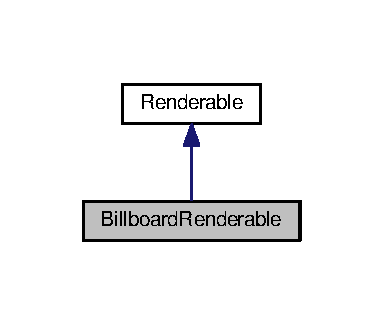
\includegraphics[width=184pt]{classBillboardRenderable__inherit__graph}
\end{center}
\end{figure}


Collaboration diagram for Billboard\+Renderable\+:\nopagebreak
\begin{figure}[H]
\begin{center}
\leavevmode
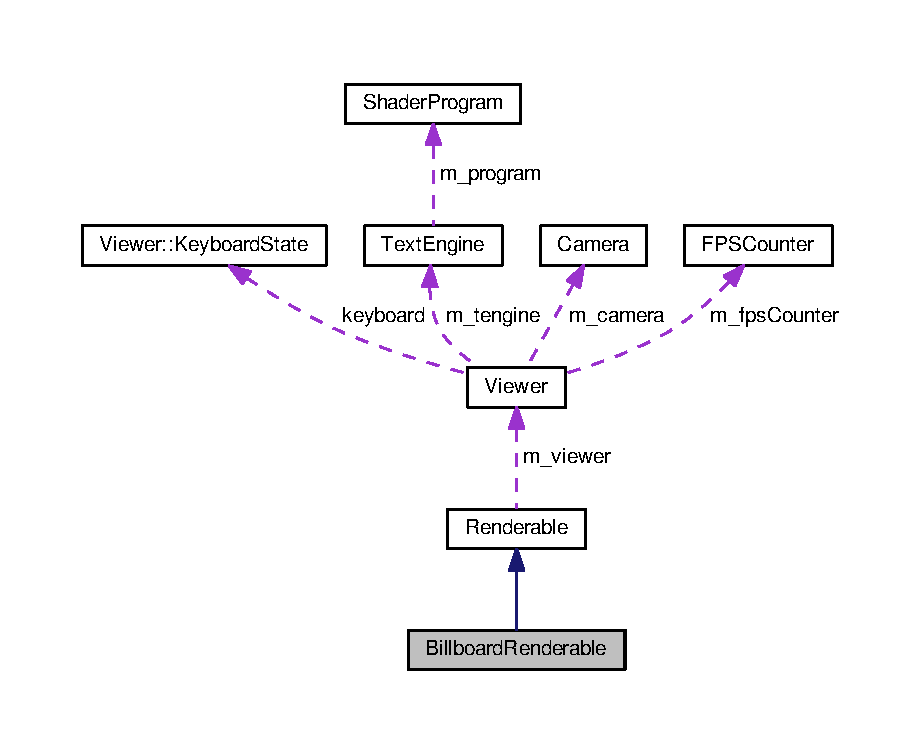
\includegraphics[width=350pt]{classBillboardRenderable__coll__graph}
\end{center}
\end{figure}
\subsection*{Public Member Functions}
\begin{DoxyCompactItemize}
\item 
\hyperlink{classBillboardRenderable_aa72988fabee4a462c6390625c664e79b}{Billboard\+Renderable} (const glm\+::vec3 \&world\+Position, const glm\+::vec2 \&world\+Dimension, \hyperlink{ShaderProgram_8hpp_af8e4af1ad4c53875ee5d32ab7e1f4966}{Shader\+Program\+Ptr} shader\+Program)
\item 
\hyperlink{classBillboardRenderable_a8f1ddb55c695fbc5d7a45f564932b328}{$\sim$\+Billboard\+Renderable} ()
\item 
void \hyperlink{classBillboardRenderable_a204c04b9ca009d0454a8ab8f6c19fbff}{set\+Position} (const glm\+::vec3 \&world\+Position)
\item 
void \hyperlink{classBillboardRenderable_a071366e85212a146bc43f64e9aa1fb5a}{set\+Dimension} (const glm\+::vec2 \&world\+Dimension)
\item 
const glm\+::vec3 \& \hyperlink{classBillboardRenderable_a981ea0b8383e18171fc56b3a1fa3c292}{get\+Position} () const 
\item 
const glm\+::vec2 \& \hyperlink{classBillboardRenderable_a2f6885a6285d6e5e8224901fa4d14cf8}{get\+Dimension} () const 
\end{DoxyCompactItemize}
\subsection*{Private Member Functions}
\begin{DoxyCompactItemize}
\item 
void \hyperlink{classBillboardRenderable_af3c5c220c558b0902acbbb5dd3f81174}{do\+\_\+draw} ()
\begin{DoxyCompactList}\small\item\em Draw virtual function. \end{DoxyCompactList}\item 
void \hyperlink{classBillboardRenderable_a99db8d2221571aed576e2f1e56ddc00e}{do\+\_\+animate} (float time)
\begin{DoxyCompactList}\small\item\em Animate virtual function. \end{DoxyCompactList}\end{DoxyCompactItemize}
\subsection*{Private Attributes}
\begin{DoxyCompactItemize}
\item 
glm\+::vec3 \hyperlink{classBillboardRenderable_aa0477db068d4c9a67aaa9031871ae8e4}{m\+\_\+position}
\item 
glm\+::vec2 \hyperlink{classBillboardRenderable_a69542c4170487272fea0bf0e207ca376}{m\+\_\+dimension}
\item 
bool \hyperlink{classBillboardRenderable_a9f034ff978eb852437ffa91cfcdc9b6e}{m\+\_\+with\+\_\+flower}
\end{DoxyCompactItemize}
\subsection*{Additional Inherited Members}


\subsection{Detailed Description}
A billboard can be more easily rendered thanks to a geometry shader. However, the geometry stage is outside the scope of the lessons. 

\subsection{Constructor \& Destructor Documentation}
\hypertarget{classBillboardRenderable_aa72988fabee4a462c6390625c664e79b}{\index{Billboard\+Renderable@{Billboard\+Renderable}!Billboard\+Renderable@{Billboard\+Renderable}}
\index{Billboard\+Renderable@{Billboard\+Renderable}!Billboard\+Renderable@{Billboard\+Renderable}}
\subsubsection[{Billboard\+Renderable}]{\setlength{\rightskip}{0pt plus 5cm}Billboard\+Renderable\+::\+Billboard\+Renderable (
\begin{DoxyParamCaption}
\item[{const glm\+::vec3 \&}]{world\+Position, }
\item[{const glm\+::vec2 \&}]{world\+Dimension, }
\item[{{\bf Shader\+Program\+Ptr}}]{shader\+Program}
\end{DoxyParamCaption}
)}}\label{classBillboardRenderable_aa72988fabee4a462c6390625c664e79b}
\hypertarget{classBillboardRenderable_a8f1ddb55c695fbc5d7a45f564932b328}{\index{Billboard\+Renderable@{Billboard\+Renderable}!````~Billboard\+Renderable@{$\sim$\+Billboard\+Renderable}}
\index{````~Billboard\+Renderable@{$\sim$\+Billboard\+Renderable}!Billboard\+Renderable@{Billboard\+Renderable}}
\subsubsection[{$\sim$\+Billboard\+Renderable}]{\setlength{\rightskip}{0pt plus 5cm}Billboard\+Renderable\+::$\sim$\+Billboard\+Renderable (
\begin{DoxyParamCaption}
{}
\end{DoxyParamCaption}
)}}\label{classBillboardRenderable_a8f1ddb55c695fbc5d7a45f564932b328}


\subsection{Member Function Documentation}
\hypertarget{classBillboardRenderable_a99db8d2221571aed576e2f1e56ddc00e}{\index{Billboard\+Renderable@{Billboard\+Renderable}!do\+\_\+animate@{do\+\_\+animate}}
\index{do\+\_\+animate@{do\+\_\+animate}!Billboard\+Renderable@{Billboard\+Renderable}}
\subsubsection[{do\+\_\+animate}]{\setlength{\rightskip}{0pt plus 5cm}void Billboard\+Renderable\+::do\+\_\+animate (
\begin{DoxyParamCaption}
\item[{float}]{time}
\end{DoxyParamCaption}
)\hspace{0.3cm}{\ttfamily [private]}, {\ttfamily [virtual]}}}\label{classBillboardRenderable_a99db8d2221571aed576e2f1e56ddc00e}
Implementation to animate this renderable. 
\begin{DoxyParams}{Parameters}
{\em time} & The current simulation time. \\
\hline
\end{DoxyParams}


Implements \hyperlink{classRenderable_aa5206322555c9dece40b21e797629b34}{Renderable}.

\hypertarget{classBillboardRenderable_af3c5c220c558b0902acbbb5dd3f81174}{\index{Billboard\+Renderable@{Billboard\+Renderable}!do\+\_\+draw@{do\+\_\+draw}}
\index{do\+\_\+draw@{do\+\_\+draw}!Billboard\+Renderable@{Billboard\+Renderable}}
\subsubsection[{do\+\_\+draw}]{\setlength{\rightskip}{0pt plus 5cm}void Billboard\+Renderable\+::do\+\_\+draw (
\begin{DoxyParamCaption}
{}
\end{DoxyParamCaption}
)\hspace{0.3cm}{\ttfamily [private]}, {\ttfamily [virtual]}}}\label{classBillboardRenderable_af3c5c220c558b0902acbbb5dd3f81174}
Implementation to draw this renderable. 

Implements \hyperlink{classRenderable_a98ab6308c1d2b56dacda7c435fb38d5b}{Renderable}.

\hypertarget{classBillboardRenderable_a2f6885a6285d6e5e8224901fa4d14cf8}{\index{Billboard\+Renderable@{Billboard\+Renderable}!get\+Dimension@{get\+Dimension}}
\index{get\+Dimension@{get\+Dimension}!Billboard\+Renderable@{Billboard\+Renderable}}
\subsubsection[{get\+Dimension}]{\setlength{\rightskip}{0pt plus 5cm}const glm\+::vec2\& Billboard\+Renderable\+::get\+Dimension (
\begin{DoxyParamCaption}
{}
\end{DoxyParamCaption}
) const}}\label{classBillboardRenderable_a2f6885a6285d6e5e8224901fa4d14cf8}
\hypertarget{classBillboardRenderable_a981ea0b8383e18171fc56b3a1fa3c292}{\index{Billboard\+Renderable@{Billboard\+Renderable}!get\+Position@{get\+Position}}
\index{get\+Position@{get\+Position}!Billboard\+Renderable@{Billboard\+Renderable}}
\subsubsection[{get\+Position}]{\setlength{\rightskip}{0pt plus 5cm}const glm\+::vec3\& Billboard\+Renderable\+::get\+Position (
\begin{DoxyParamCaption}
{}
\end{DoxyParamCaption}
) const}}\label{classBillboardRenderable_a981ea0b8383e18171fc56b3a1fa3c292}
\hypertarget{classBillboardRenderable_a071366e85212a146bc43f64e9aa1fb5a}{\index{Billboard\+Renderable@{Billboard\+Renderable}!set\+Dimension@{set\+Dimension}}
\index{set\+Dimension@{set\+Dimension}!Billboard\+Renderable@{Billboard\+Renderable}}
\subsubsection[{set\+Dimension}]{\setlength{\rightskip}{0pt plus 5cm}void Billboard\+Renderable\+::set\+Dimension (
\begin{DoxyParamCaption}
\item[{const glm\+::vec2 \&}]{world\+Dimension}
\end{DoxyParamCaption}
)}}\label{classBillboardRenderable_a071366e85212a146bc43f64e9aa1fb5a}
\hypertarget{classBillboardRenderable_a204c04b9ca009d0454a8ab8f6c19fbff}{\index{Billboard\+Renderable@{Billboard\+Renderable}!set\+Position@{set\+Position}}
\index{set\+Position@{set\+Position}!Billboard\+Renderable@{Billboard\+Renderable}}
\subsubsection[{set\+Position}]{\setlength{\rightskip}{0pt plus 5cm}void Billboard\+Renderable\+::set\+Position (
\begin{DoxyParamCaption}
\item[{const glm\+::vec3 \&}]{world\+Position}
\end{DoxyParamCaption}
)}}\label{classBillboardRenderable_a204c04b9ca009d0454a8ab8f6c19fbff}


\subsection{Member Data Documentation}
\hypertarget{classBillboardRenderable_a69542c4170487272fea0bf0e207ca376}{\index{Billboard\+Renderable@{Billboard\+Renderable}!m\+\_\+dimension@{m\+\_\+dimension}}
\index{m\+\_\+dimension@{m\+\_\+dimension}!Billboard\+Renderable@{Billboard\+Renderable}}
\subsubsection[{m\+\_\+dimension}]{\setlength{\rightskip}{0pt plus 5cm}glm\+::vec2 Billboard\+Renderable\+::m\+\_\+dimension\hspace{0.3cm}{\ttfamily [private]}}}\label{classBillboardRenderable_a69542c4170487272fea0bf0e207ca376}
\hypertarget{classBillboardRenderable_aa0477db068d4c9a67aaa9031871ae8e4}{\index{Billboard\+Renderable@{Billboard\+Renderable}!m\+\_\+position@{m\+\_\+position}}
\index{m\+\_\+position@{m\+\_\+position}!Billboard\+Renderable@{Billboard\+Renderable}}
\subsubsection[{m\+\_\+position}]{\setlength{\rightskip}{0pt plus 5cm}glm\+::vec3 Billboard\+Renderable\+::m\+\_\+position\hspace{0.3cm}{\ttfamily [private]}}}\label{classBillboardRenderable_aa0477db068d4c9a67aaa9031871ae8e4}
\hypertarget{classBillboardRenderable_a9f034ff978eb852437ffa91cfcdc9b6e}{\index{Billboard\+Renderable@{Billboard\+Renderable}!m\+\_\+with\+\_\+flower@{m\+\_\+with\+\_\+flower}}
\index{m\+\_\+with\+\_\+flower@{m\+\_\+with\+\_\+flower}!Billboard\+Renderable@{Billboard\+Renderable}}
\subsubsection[{m\+\_\+with\+\_\+flower}]{\setlength{\rightskip}{0pt plus 5cm}bool Billboard\+Renderable\+::m\+\_\+with\+\_\+flower\hspace{0.3cm}{\ttfamily [private]}}}\label{classBillboardRenderable_a9f034ff978eb852437ffa91cfcdc9b6e}


The documentation for this class was generated from the following file\+:\begin{DoxyCompactItemize}
\item 
/home/chardon/\+Depot/ensimag/2\+A\+\_\+\+G3\+D/practicals/teacher\+Source/include/texturing/\hyperlink{BillboardRenderable_8hpp}{Billboard\+Renderable.\+hpp}\end{DoxyCompactItemize}

\hypertarget{classCamera}{\section{Camera Class Reference}
\label{classCamera}\index{Camera@{Camera}}
}


Manage the \hyperlink{classCamera}{Camera}.  




{\ttfamily \#include $<$Camera.\+hpp$>$}

\subsection*{Public Types}
\begin{DoxyCompactItemize}
\item 
enum \hyperlink{classCamera_a39b92a45686a6f858a3405ee34a95cfa}{C\+A\+M\+E\+R\+A\+\_\+\+M\+O\+U\+S\+E\+\_\+\+B\+E\+H\+A\+V\+I\+O\+R} \{ \hyperlink{classCamera_a39b92a45686a6f858a3405ee34a95cfaa8554ee8f8de95ea3a84d77e3e8345d1c}{A\+R\+C\+B\+A\+L\+L\+\_\+\+B\+E\+H\+A\+V\+I\+O\+R}, 
\hyperlink{classCamera_a39b92a45686a6f858a3405ee34a95cfaa37a95995e7b876b0b9994a131da60717}{S\+P\+A\+C\+E\+S\+H\+I\+P\+\_\+\+B\+E\+H\+A\+V\+I\+O\+R}
 \}
\begin{DoxyCompactList}\small\item\em Reaction to mouse displacement. \end{DoxyCompactList}\end{DoxyCompactItemize}
\subsection*{Public Member Functions}
\begin{DoxyCompactItemize}
\item 
\hyperlink{classCamera_a01f94c3543f56ede7af49dc778f19331}{Camera} ()
\begin{DoxyCompactList}\small\item\em Construction. \end{DoxyCompactList}\item 
\hyperlink{classCamera_ad1897942d0ccf91052386388a497349f}{$\sim$\+Camera} ()
\begin{DoxyCompactList}\small\item\em Destruction. \end{DoxyCompactList}\item 
void \hyperlink{classCamera_aff5389801d0c6e32c2627db0c63b9c24}{animate} (float time)
\begin{DoxyCompactList}\small\item\em Animate the camera. \end{DoxyCompactList}\end{DoxyCompactItemize}
\begin{Indent}{\bf Camera View Matrix}\par
{\em Set of methods which interact with the camera view matrix. This matrix which determines the camera frame in the world coordinates, i.\+e. the way the camera is positioned and oriented. }\begin{DoxyCompactItemize}
\item 
const glm\+::mat4 \& \hyperlink{classCamera_aba6abae81f71ffdc830a0c45a6910c76}{view\+Matrix} () const 
\begin{DoxyCompactList}\small\item\em Read access to the view matrix. \end{DoxyCompactList}\item 
void \hyperlink{classCamera_a9b4e9d0087f56802ec4d684ea9665e16}{set\+View\+Matrix} (const glm\+::mat4 \&view)
\begin{DoxyCompactList}\small\item\em Write to the view matrix. \end{DoxyCompactList}\item 
glm\+::vec3 \hyperlink{classCamera_ad741cb975e8ea88698ed1b0216a0bb82}{get\+Position} () const 
\begin{DoxyCompactList}\small\item\em Read access to the camera world position. \end{DoxyCompactList}\item 
glm\+::vec3 \hyperlink{classCamera_af8c18525d561cda9757413550436f5ca}{get\+Right} () const 
\begin{DoxyCompactList}\small\item\em Read access to the camera right direction. \end{DoxyCompactList}\item 
glm\+::vec3 \hyperlink{classCamera_a64b7a4bf8c463fd6ba5165d632d54a8e}{get\+Up} () const 
\begin{DoxyCompactList}\small\item\em Read access to the camera up direction. \end{DoxyCompactList}\item 
glm\+::vec3 \hyperlink{classCamera_aab4704e0cfa1fb4153658f129d806e78}{get\+Forward} () const 
\begin{DoxyCompactList}\small\item\em Read access to the camera forward direction. \end{DoxyCompactList}\item 
void \hyperlink{classCamera_ab7ebcdd5020d8057f1df3bdb33bac456}{set\+Position} (const glm\+::vec3 \&pos)
\begin{DoxyCompactList}\small\item\em Set the camera world position. \end{DoxyCompactList}\item 
void \hyperlink{classCamera_a02cf8fe9d3413fcb1f95a14ef02da9a3}{set\+Right} (const glm\+::vec3 \&right)
\begin{DoxyCompactList}\small\item\em Set the camera right direction. \end{DoxyCompactList}\item 
void \hyperlink{classCamera_acd252404a7ef31e327af15710bd433a4}{set\+Up} (const glm\+::vec3 \&up)
\begin{DoxyCompactList}\small\item\em Set the camera up direction. \end{DoxyCompactList}\item 
void \hyperlink{classCamera_acb3d907db2b33b09c4861e215e2e21eb}{set\+Forward} (const glm\+::vec3 \&forward)
\begin{DoxyCompactList}\small\item\em Set the camera up direction. \end{DoxyCompactList}\end{DoxyCompactItemize}
\end{Indent}
\begin{Indent}{\bf Camera Projection Matrix}\par
{\em Set of methods which interact with the projection matrix. This matrix determine how a scene is projected on a 2\+D image that will be displayed on screen. }\begin{DoxyCompactItemize}
\item 
const glm\+::mat4 \& \hyperlink{classCamera_adeda5ac08b751d6122d5f280769617a1}{projection\+Matrix} () const 
\begin{DoxyCompactList}\small\item\em Read access to the camera projection matrix. \end{DoxyCompactList}\item 
void \hyperlink{classCamera_a25474205988645b3792f1c6cffad95af}{set\+Projection\+Matrix} (const glm\+::mat4 \&projection)
\begin{DoxyCompactList}\small\item\em Write to the projection matrix of the camera. \end{DoxyCompactList}\item 
float \hyperlink{classCamera_aa2af35287b83a29333b0ae51ebaa2f4b}{fov} () const 
\begin{DoxyCompactList}\small\item\em Get the camera field of view. \end{DoxyCompactList}\item 
float \hyperlink{classCamera_aa7757f7ff602b864472fe6be5c7a23ac}{ratio} () const 
\begin{DoxyCompactList}\small\item\em Get the camera ratio. \end{DoxyCompactList}\item 
float \hyperlink{classCamera_ae2231c2ee1a4a356ef8a7e1003f04998}{znear} () const 
\begin{DoxyCompactList}\small\item\em Get the near clipping plane. \end{DoxyCompactList}\item 
float \hyperlink{classCamera_a2dba7a46727c9db0ee663751e0d4d2b1}{zfar} () const 
\begin{DoxyCompactList}\small\item\em Get the far clipping plane. \end{DoxyCompactList}\item 
void \hyperlink{classCamera_a06d62ccd30da0b6c46a837ee67c5a6b8}{set\+Fov} (const float \&v)
\begin{DoxyCompactList}\small\item\em Define the field of view. \end{DoxyCompactList}\item 
void \hyperlink{classCamera_aa191430dcb1e9f7ab01251d3081913a6}{set\+Ratio} (const float \&v)
\begin{DoxyCompactList}\small\item\em Define the aspect ratio. \end{DoxyCompactList}\item 
void \hyperlink{classCamera_ad0f1812ed5bf995493591e1c8aff19a3}{set\+Zfar} (const float \&v)
\begin{DoxyCompactList}\small\item\em Define the far clipping plane. \end{DoxyCompactList}\item 
void \hyperlink{classCamera_a86cc28211d99e582cdbeba609c644208}{set\+Znear} (const float \&v)
\begin{DoxyCompactList}\small\item\em Define the near clipping plane. \end{DoxyCompactList}\end{DoxyCompactItemize}
\end{Indent}
\begin{Indent}{\bf Mouse Control}\par
{\em Control the camera with the mouse. }\begin{DoxyCompactItemize}
\item 
\hyperlink{classCamera_a39b92a45686a6f858a3405ee34a95cfa}{C\+A\+M\+E\+R\+A\+\_\+\+M\+O\+U\+S\+E\+\_\+\+B\+E\+H\+A\+V\+I\+O\+R} \hyperlink{classCamera_a35b61591c2a26f707c95e2a17c00ec70}{get\+Mouse\+Behavior} () const 
\begin{DoxyCompactList}\small\item\em Get the mouse behavior. \end{DoxyCompactList}\item 
void \hyperlink{classCamera_ae2b1471c97d7709358ccd754e68c1ca6}{set\+Mouse\+Behavior} (const \hyperlink{classCamera_a39b92a45686a6f858a3405ee34a95cfa}{C\+A\+M\+E\+R\+A\+\_\+\+M\+O\+U\+S\+E\+\_\+\+B\+E\+H\+A\+V\+I\+O\+R} \&v)
\begin{DoxyCompactList}\small\item\em Set the mouse behavior. \end{DoxyCompactList}\item 
void \hyperlink{classCamera_a21e660f7345ef5cfb347ac5c78e0c491}{update} (float dx, float dy)
\begin{DoxyCompactList}\small\item\em Update the camera view in reaction to a mouse displacement. \end{DoxyCompactList}\end{DoxyCompactItemize}
\end{Indent}
\subsection*{Private Attributes}
\begin{Indent}{\bf Private members}\par
\begin{DoxyCompactItemize}
\item 
\hyperlink{classCamera_a39b92a45686a6f858a3405ee34a95cfa}{C\+A\+M\+E\+R\+A\+\_\+\+M\+O\+U\+S\+E\+\_\+\+B\+E\+H\+A\+V\+I\+O\+R} \hyperlink{classCamera_a4aa308842db545da7732c5fe306be934}{m\+\_\+mouse\+Behavior}
\item 
float \hyperlink{classCamera_aa404a4e057fa16fb82ce8668d7a661b6}{m\+\_\+fov}
\item 
float \hyperlink{classCamera_aac7338a3de62c4f1b78a5553ae642c27}{m\+\_\+ratio}
\item 
float \hyperlink{classCamera_a3e01bcfeedeb9ee1950bca467dcd2185}{m\+\_\+znear}
\item 
float \hyperlink{classCamera_a2a5760d0aff07b0dd1039ee7ccc2596c}{m\+\_\+zfar}
\item 
glm\+::mat4 \hyperlink{classCamera_ad0e8cb00cfe1dd9a2aabd7ed92bde2e4}{m\+\_\+view}
\item 
glm\+::mat4 \hyperlink{classCamera_a32746f033de65f9bf0d3e6823b77f339}{m\+\_\+projection}
\end{DoxyCompactItemize}
\end{Indent}


\subsection{Detailed Description}
We consider a camera to be defined by two 4x4 matrices\+:
\begin{DoxyItemize}
\item the view matrix
\item the projection matrix.
\end{DoxyItemize}

The view matrix defines the position and the orientation of the camera in the world coordinates. It is represented as follow\+: \begin{TabularC}{4}
\hline
\rowcolor{lightgray}{\bf Column 0 }&{\bf Column 1 }&{\bf Column 2 }&{\bf Column 3  }\\\cline{1-4}
X0 &X1 &X2 &P0 \\\cline{1-4}
Y0 &Y1 &Y2 &P1 \\\cline{1-4}
Z0 &Z1 &Z2 &P2 \\\cline{1-4}
0 &0 &0 &1 \\\cline{1-4}
\end{TabularC}
X=(X0,X1,X2), Y=(Y0,Y1,Y2) and Z=(Z0,Z1,Z2) represent the right, up, and backward direction of the camera in the world coordinates. The point P=(P0,P1,P2) is the position of the world origin in the camera frame (X,Y,Z). Thus, the point (-\/dot(P,X), -\/dot(P,Y), -\/dot(P,Z)) is the position of the camera in the world coordinates.

The projection matrix defines the way the scene viewed by the camera is transformed (projected) to a 2\+D image that will be displayed on screen. To compute this matrix, we need ratio of the 2\+D image, the field of view and the far and near cutting plane distances. 

\subsection{Member Enumeration Documentation}
\hypertarget{classCamera_a39b92a45686a6f858a3405ee34a95cfa}{\index{Camera@{Camera}!C\+A\+M\+E\+R\+A\+\_\+\+M\+O\+U\+S\+E\+\_\+\+B\+E\+H\+A\+V\+I\+O\+R@{C\+A\+M\+E\+R\+A\+\_\+\+M\+O\+U\+S\+E\+\_\+\+B\+E\+H\+A\+V\+I\+O\+R}}
\index{C\+A\+M\+E\+R\+A\+\_\+\+M\+O\+U\+S\+E\+\_\+\+B\+E\+H\+A\+V\+I\+O\+R@{C\+A\+M\+E\+R\+A\+\_\+\+M\+O\+U\+S\+E\+\_\+\+B\+E\+H\+A\+V\+I\+O\+R}!Camera@{Camera}}
\subsubsection[{C\+A\+M\+E\+R\+A\+\_\+\+M\+O\+U\+S\+E\+\_\+\+B\+E\+H\+A\+V\+I\+O\+R}]{\setlength{\rightskip}{0pt plus 5cm}enum {\bf Camera\+::\+C\+A\+M\+E\+R\+A\+\_\+\+M\+O\+U\+S\+E\+\_\+\+B\+E\+H\+A\+V\+I\+O\+R}}}\label{classCamera_a39b92a45686a6f858a3405ee34a95cfa}
This enumeration specifies the different kind of reaction to a mouse displacement. \begin{Desc}
\item[Enumerator]\par
\begin{description}
\index{A\+R\+C\+B\+A\+L\+L\+\_\+\+B\+E\+H\+A\+V\+I\+O\+R@{A\+R\+C\+B\+A\+L\+L\+\_\+\+B\+E\+H\+A\+V\+I\+O\+R}!Camera@{Camera}}\index{Camera@{Camera}!A\+R\+C\+B\+A\+L\+L\+\_\+\+B\+E\+H\+A\+V\+I\+O\+R@{A\+R\+C\+B\+A\+L\+L\+\_\+\+B\+E\+H\+A\+V\+I\+O\+R}}\item[{\em 
\hypertarget{classCamera_a39b92a45686a6f858a3405ee34a95cfaa8554ee8f8de95ea3a84d77e3e8345d1c}{A\+R\+C\+B\+A\+L\+L\+\_\+\+B\+E\+H\+A\+V\+I\+O\+R}\label{classCamera_a39b92a45686a6f858a3405ee34a95cfaa8554ee8f8de95ea3a84d77e3e8345d1c}
}]The view matrix is modified to turn the camera around the world origin. \index{S\+P\+A\+C\+E\+S\+H\+I\+P\+\_\+\+B\+E\+H\+A\+V\+I\+O\+R@{S\+P\+A\+C\+E\+S\+H\+I\+P\+\_\+\+B\+E\+H\+A\+V\+I\+O\+R}!Camera@{Camera}}\index{Camera@{Camera}!S\+P\+A\+C\+E\+S\+H\+I\+P\+\_\+\+B\+E\+H\+A\+V\+I\+O\+R@{S\+P\+A\+C\+E\+S\+H\+I\+P\+\_\+\+B\+E\+H\+A\+V\+I\+O\+R}}\item[{\em 
\hypertarget{classCamera_a39b92a45686a6f858a3405ee34a95cfaa37a95995e7b876b0b9994a131da60717}{S\+P\+A\+C\+E\+S\+H\+I\+P\+\_\+\+B\+E\+H\+A\+V\+I\+O\+R}\label{classCamera_a39b92a45686a6f858a3405ee34a95cfaa37a95995e7b876b0b9994a131da60717}
}]The view matrix is modified to point its 'nose' in the direction pointed by the mouse. \end{description}
\end{Desc}


\subsection{Constructor \& Destructor Documentation}
\hypertarget{classCamera_a01f94c3543f56ede7af49dc778f19331}{\index{Camera@{Camera}!Camera@{Camera}}
\index{Camera@{Camera}!Camera@{Camera}}
\subsubsection[{Camera}]{\setlength{\rightskip}{0pt plus 5cm}Camera\+::\+Camera (
\begin{DoxyParamCaption}
{}
\end{DoxyParamCaption}
)}}\label{classCamera_a01f94c3543f56ede7af49dc778f19331}
Create a default camera located at (0,0,-\/5), looking at the position (0,0,0), with an up vector equals to (0,1,0). The default camera behavior is \hyperlink{classCamera_a39b92a45686a6f858a3405ee34a95cfaa8554ee8f8de95ea3a84d77e3e8345d1c}{Camera\+::\+A\+R\+C\+B\+A\+L\+L\+\_\+\+B\+E\+H\+A\+V\+I\+O\+R}. If such default behavior does not suit you, feel free to change it in the implementation file. \hypertarget{classCamera_ad1897942d0ccf91052386388a497349f}{\index{Camera@{Camera}!````~Camera@{$\sim$\+Camera}}
\index{````~Camera@{$\sim$\+Camera}!Camera@{Camera}}
\subsubsection[{$\sim$\+Camera}]{\setlength{\rightskip}{0pt plus 5cm}Camera\+::$\sim$\+Camera (
\begin{DoxyParamCaption}
{}
\end{DoxyParamCaption}
)}}\label{classCamera_ad1897942d0ccf91052386388a497349f}
Instance destruction. 

\subsection{Member Function Documentation}
\hypertarget{classCamera_aff5389801d0c6e32c2627db0c63b9c24}{\index{Camera@{Camera}!animate@{animate}}
\index{animate@{animate}!Camera@{Camera}}
\subsubsection[{animate}]{\setlength{\rightskip}{0pt plus 5cm}void Camera\+::animate (
\begin{DoxyParamCaption}
\item[{float}]{time}
\end{DoxyParamCaption}
)}}\label{classCamera_aff5389801d0c6e32c2627db0c63b9c24}
This function is currently empty, but you can define an animation behavior here. This function is automatically called by the \hyperlink{classViewer}{Viewer} 
\begin{DoxyParams}{Parameters}
{\em time} & Current simulation time. \\
\hline
\end{DoxyParams}
\hypertarget{classCamera_aa2af35287b83a29333b0ae51ebaa2f4b}{\index{Camera@{Camera}!fov@{fov}}
\index{fov@{fov}!Camera@{Camera}}
\subsubsection[{fov}]{\setlength{\rightskip}{0pt plus 5cm}float Camera\+::fov (
\begin{DoxyParamCaption}
{}
\end{DoxyParamCaption}
) const}}\label{classCamera_aa2af35287b83a29333b0ae51ebaa2f4b}
Get the field of view of the camera, also known as the camera angle. \begin{DoxyReturn}{Returns}
The camera fov. 
\end{DoxyReturn}
\hypertarget{classCamera_aab4704e0cfa1fb4153658f129d806e78}{\index{Camera@{Camera}!get\+Forward@{get\+Forward}}
\index{get\+Forward@{get\+Forward}!Camera@{Camera}}
\subsubsection[{get\+Forward}]{\setlength{\rightskip}{0pt plus 5cm}glm\+::vec3 Camera\+::get\+Forward (
\begin{DoxyParamCaption}
{}
\end{DoxyParamCaption}
) const}}\label{classCamera_aab4704e0cfa1fb4153658f129d806e78}
Allow a read-\/only access to the forward direction of the camera in world coordinates. This direction corresponds to the (-\/\+Z) direction of the camera local frame, also known as the 'looking direction'.

\begin{DoxyReturn}{Returns}
The camera forward direction. 
\end{DoxyReturn}
\hypertarget{classCamera_a35b61591c2a26f707c95e2a17c00ec70}{\index{Camera@{Camera}!get\+Mouse\+Behavior@{get\+Mouse\+Behavior}}
\index{get\+Mouse\+Behavior@{get\+Mouse\+Behavior}!Camera@{Camera}}
\subsubsection[{get\+Mouse\+Behavior}]{\setlength{\rightskip}{0pt plus 5cm}{\bf C\+A\+M\+E\+R\+A\+\_\+\+M\+O\+U\+S\+E\+\_\+\+B\+E\+H\+A\+V\+I\+O\+R} Camera\+::get\+Mouse\+Behavior (
\begin{DoxyParamCaption}
{}
\end{DoxyParamCaption}
) const}}\label{classCamera_a35b61591c2a26f707c95e2a17c00ec70}
Access to the mouse behavior currently used by the update( dx, dy ) function. \begin{DoxyReturn}{Returns}
The mouse behavior. 
\end{DoxyReturn}
\hypertarget{classCamera_ad741cb975e8ea88698ed1b0216a0bb82}{\index{Camera@{Camera}!get\+Position@{get\+Position}}
\index{get\+Position@{get\+Position}!Camera@{Camera}}
\subsubsection[{get\+Position}]{\setlength{\rightskip}{0pt plus 5cm}glm\+::vec3 Camera\+::get\+Position (
\begin{DoxyParamCaption}
{}
\end{DoxyParamCaption}
) const}}\label{classCamera_ad741cb975e8ea88698ed1b0216a0bb82}
Allow a read-\/only access to the camera position in world coordinates. \begin{DoxyReturn}{Returns}
The camera position. 
\end{DoxyReturn}
\hypertarget{classCamera_af8c18525d561cda9757413550436f5ca}{\index{Camera@{Camera}!get\+Right@{get\+Right}}
\index{get\+Right@{get\+Right}!Camera@{Camera}}
\subsubsection[{get\+Right}]{\setlength{\rightskip}{0pt plus 5cm}glm\+::vec3 Camera\+::get\+Right (
\begin{DoxyParamCaption}
{}
\end{DoxyParamCaption}
) const}}\label{classCamera_af8c18525d561cda9757413550436f5ca}
Allow a read-\/only access to the right direction of the camera in world coordinates. This direction corresponds to the (+\+X) direction of the camera local frame.

\begin{DoxyReturn}{Returns}
The camera right direction 
\end{DoxyReturn}
\hypertarget{classCamera_a64b7a4bf8c463fd6ba5165d632d54a8e}{\index{Camera@{Camera}!get\+Up@{get\+Up}}
\index{get\+Up@{get\+Up}!Camera@{Camera}}
\subsubsection[{get\+Up}]{\setlength{\rightskip}{0pt plus 5cm}glm\+::vec3 Camera\+::get\+Up (
\begin{DoxyParamCaption}
{}
\end{DoxyParamCaption}
) const}}\label{classCamera_a64b7a4bf8c463fd6ba5165d632d54a8e}
Allow a read-\/only access to the up direction of the camera in world coordinates. This direction corresponds to the (+\+Y) direction of the camera local frame.

\begin{DoxyReturn}{Returns}
The camera up direction. 
\end{DoxyReturn}
\hypertarget{classCamera_adeda5ac08b751d6122d5f280769617a1}{\index{Camera@{Camera}!projection\+Matrix@{projection\+Matrix}}
\index{projection\+Matrix@{projection\+Matrix}!Camera@{Camera}}
\subsubsection[{projection\+Matrix}]{\setlength{\rightskip}{0pt plus 5cm}const glm\+::mat4\& Camera\+::projection\+Matrix (
\begin{DoxyParamCaption}
{}
\end{DoxyParamCaption}
) const}}\label{classCamera_adeda5ac08b751d6122d5f280769617a1}
Allow a read-\/only access to the camera projection matrix. This matrix defines how to go from the pixel coordinates to the screen coordinates.

\begin{DoxyReturn}{Returns}
The projection matrix. 
\end{DoxyReturn}
\hypertarget{classCamera_aa7757f7ff602b864472fe6be5c7a23ac}{\index{Camera@{Camera}!ratio@{ratio}}
\index{ratio@{ratio}!Camera@{Camera}}
\subsubsection[{ratio}]{\setlength{\rightskip}{0pt plus 5cm}float Camera\+::ratio (
\begin{DoxyParamCaption}
{}
\end{DoxyParamCaption}
) const}}\label{classCamera_aa7757f7ff602b864472fe6be5c7a23ac}
The camera ratio is the length ratio of the image taken by this camera. This ratio is meant to be equal to the width of the display window divided by its height. This ratio is also know as the aspect ratio.

\begin{DoxyReturn}{Returns}
The length ratio of the image taken by this camera. 
\end{DoxyReturn}
\hypertarget{classCamera_acb3d907db2b33b09c4861e215e2e21eb}{\index{Camera@{Camera}!set\+Forward@{set\+Forward}}
\index{set\+Forward@{set\+Forward}!Camera@{Camera}}
\subsubsection[{set\+Forward}]{\setlength{\rightskip}{0pt plus 5cm}void Camera\+::set\+Forward (
\begin{DoxyParamCaption}
\item[{const glm\+::vec3 \&}]{forward}
\end{DoxyParamCaption}
)}}\label{classCamera_acb3d907db2b33b09c4861e215e2e21eb}
Set the camera forward (-\/\+Z) direction in world coordinates. 
\begin{DoxyParams}{Parameters}
{\em forward} & New camera forward direction in world coordinates. \\
\hline
\end{DoxyParams}
\hypertarget{classCamera_a06d62ccd30da0b6c46a837ee67c5a6b8}{\index{Camera@{Camera}!set\+Fov@{set\+Fov}}
\index{set\+Fov@{set\+Fov}!Camera@{Camera}}
\subsubsection[{set\+Fov}]{\setlength{\rightskip}{0pt plus 5cm}void Camera\+::set\+Fov (
\begin{DoxyParamCaption}
\item[{const float \&}]{v}
\end{DoxyParamCaption}
)}}\label{classCamera_a06d62ccd30da0b6c46a837ee67c5a6b8}
Set the camera field of view. We consider 1.\+04 is a good start to find a custom fov. 
\begin{DoxyParams}{Parameters}
{\em v} & The new field of view. \\
\hline
\end{DoxyParams}
\hypertarget{classCamera_ae2b1471c97d7709358ccd754e68c1ca6}{\index{Camera@{Camera}!set\+Mouse\+Behavior@{set\+Mouse\+Behavior}}
\index{set\+Mouse\+Behavior@{set\+Mouse\+Behavior}!Camera@{Camera}}
\subsubsection[{set\+Mouse\+Behavior}]{\setlength{\rightskip}{0pt plus 5cm}void Camera\+::set\+Mouse\+Behavior (
\begin{DoxyParamCaption}
\item[{const {\bf C\+A\+M\+E\+R\+A\+\_\+\+M\+O\+U\+S\+E\+\_\+\+B\+E\+H\+A\+V\+I\+O\+R} \&}]{v}
\end{DoxyParamCaption}
)}}\label{classCamera_ae2b1471c97d7709358ccd754e68c1ca6}
Set the new mouse behavior of the camera, that will be used by the update( dx, dy ) function. 
\begin{DoxyParams}{Parameters}
{\em v} & The new behavior. \\
\hline
\end{DoxyParams}
\hypertarget{classCamera_ab7ebcdd5020d8057f1df3bdb33bac456}{\index{Camera@{Camera}!set\+Position@{set\+Position}}
\index{set\+Position@{set\+Position}!Camera@{Camera}}
\subsubsection[{set\+Position}]{\setlength{\rightskip}{0pt plus 5cm}void Camera\+::set\+Position (
\begin{DoxyParamCaption}
\item[{const glm\+::vec3 \&}]{pos}
\end{DoxyParamCaption}
)}}\label{classCamera_ab7ebcdd5020d8057f1df3bdb33bac456}
Set the camera position in world coordinates. 
\begin{DoxyParams}{Parameters}
{\em pos} & New camera world position. \\
\hline
\end{DoxyParams}
\hypertarget{classCamera_a25474205988645b3792f1c6cffad95af}{\index{Camera@{Camera}!set\+Projection\+Matrix@{set\+Projection\+Matrix}}
\index{set\+Projection\+Matrix@{set\+Projection\+Matrix}!Camera@{Camera}}
\subsubsection[{set\+Projection\+Matrix}]{\setlength{\rightskip}{0pt plus 5cm}void Camera\+::set\+Projection\+Matrix (
\begin{DoxyParamCaption}
\item[{const glm\+::mat4 \&}]{projection}
\end{DoxyParamCaption}
)}}\label{classCamera_a25474205988645b3792f1c6cffad95af}
Allow to write to the projection matrix of the camera. 
\begin{DoxyParams}{Parameters}
{\em projection} & The new projection matrix used by this camera. \\
\hline
\end{DoxyParams}
\hypertarget{classCamera_aa191430dcb1e9f7ab01251d3081913a6}{\index{Camera@{Camera}!set\+Ratio@{set\+Ratio}}
\index{set\+Ratio@{set\+Ratio}!Camera@{Camera}}
\subsubsection[{set\+Ratio}]{\setlength{\rightskip}{0pt plus 5cm}void Camera\+::set\+Ratio (
\begin{DoxyParamCaption}
\item[{const float \&}]{v}
\end{DoxyParamCaption}
)}}\label{classCamera_aa191430dcb1e9f7ab01251d3081913a6}
Set the camera aspect ratio. Generally, this is done at each window resize. The \hyperlink{classViewer}{Viewer} automatically call this method on its camera when its window is resized. 
\begin{DoxyParams}{Parameters}
{\em v} & The new aspect ratio (width / height) \\
\hline
\end{DoxyParams}
\hypertarget{classCamera_a02cf8fe9d3413fcb1f95a14ef02da9a3}{\index{Camera@{Camera}!set\+Right@{set\+Right}}
\index{set\+Right@{set\+Right}!Camera@{Camera}}
\subsubsection[{set\+Right}]{\setlength{\rightskip}{0pt plus 5cm}void Camera\+::set\+Right (
\begin{DoxyParamCaption}
\item[{const glm\+::vec3 \&}]{right}
\end{DoxyParamCaption}
)}}\label{classCamera_a02cf8fe9d3413fcb1f95a14ef02da9a3}
Set the camera right direction in world coordinates. 
\begin{DoxyParams}{Parameters}
{\em right} & New camera right axis in world coordinates. \\
\hline
\end{DoxyParams}
\hypertarget{classCamera_acd252404a7ef31e327af15710bd433a4}{\index{Camera@{Camera}!set\+Up@{set\+Up}}
\index{set\+Up@{set\+Up}!Camera@{Camera}}
\subsubsection[{set\+Up}]{\setlength{\rightskip}{0pt plus 5cm}void Camera\+::set\+Up (
\begin{DoxyParamCaption}
\item[{const glm\+::vec3 \&}]{up}
\end{DoxyParamCaption}
)}}\label{classCamera_acd252404a7ef31e327af15710bd433a4}
Set the camera up direction in world coordinates. 
\begin{DoxyParams}{Parameters}
{\em up} & New camera up axis in world coordinates. \\
\hline
\end{DoxyParams}
\hypertarget{classCamera_a9b4e9d0087f56802ec4d684ea9665e16}{\index{Camera@{Camera}!set\+View\+Matrix@{set\+View\+Matrix}}
\index{set\+View\+Matrix@{set\+View\+Matrix}!Camera@{Camera}}
\subsubsection[{set\+View\+Matrix}]{\setlength{\rightskip}{0pt plus 5cm}void Camera\+::set\+View\+Matrix (
\begin{DoxyParamCaption}
\item[{const glm\+::mat4 \&}]{view}
\end{DoxyParamCaption}
)}}\label{classCamera_a9b4e9d0087f56802ec4d684ea9665e16}
Allow to write to the view matrix. This could be useful if the view matrix is handled in another place than in the camera. 
\begin{DoxyParams}{Parameters}
{\em view} & The new view matrix. \\
\hline
\end{DoxyParams}
\hypertarget{classCamera_ad0f1812ed5bf995493591e1c8aff19a3}{\index{Camera@{Camera}!set\+Zfar@{set\+Zfar}}
\index{set\+Zfar@{set\+Zfar}!Camera@{Camera}}
\subsubsection[{set\+Zfar}]{\setlength{\rightskip}{0pt plus 5cm}void Camera\+::set\+Zfar (
\begin{DoxyParamCaption}
\item[{const float \&}]{v}
\end{DoxyParamCaption}
)}}\label{classCamera_ad0f1812ed5bf995493591e1c8aff19a3}
Set the far clipping plane at the specified distance. 
\begin{DoxyParams}{Parameters}
{\em v} & The far clipping plane distance. \\
\hline
\end{DoxyParams}
\hypertarget{classCamera_a86cc28211d99e582cdbeba609c644208}{\index{Camera@{Camera}!set\+Znear@{set\+Znear}}
\index{set\+Znear@{set\+Znear}!Camera@{Camera}}
\subsubsection[{set\+Znear}]{\setlength{\rightskip}{0pt plus 5cm}void Camera\+::set\+Znear (
\begin{DoxyParamCaption}
\item[{const float \&}]{v}
\end{DoxyParamCaption}
)}}\label{classCamera_a86cc28211d99e582cdbeba609c644208}
Set the near clipping plane at the specified distance. 
\begin{DoxyParams}{Parameters}
{\em v} & The near clipping plane distance. \\
\hline
\end{DoxyParams}
\hypertarget{classCamera_a21e660f7345ef5cfb347ac5c78e0c491}{\index{Camera@{Camera}!update@{update}}
\index{update@{update}!Camera@{Camera}}
\subsubsection[{update}]{\setlength{\rightskip}{0pt plus 5cm}void Camera\+::update (
\begin{DoxyParamCaption}
\item[{float}]{dx, }
\item[{float}]{dy}
\end{DoxyParamCaption}
)}}\label{classCamera_a21e660f7345ef5cfb347ac5c78e0c491}
Change the camera view matrix according to the current mouse behavior. 
\begin{DoxyParams}{Parameters}
{\em dx} & Mouse x displacement. \\
\hline
{\em dy} & Mouse y displacement. \\
\hline
\end{DoxyParams}
\hypertarget{classCamera_aba6abae81f71ffdc830a0c45a6910c76}{\index{Camera@{Camera}!view\+Matrix@{view\+Matrix}}
\index{view\+Matrix@{view\+Matrix}!Camera@{Camera}}
\subsubsection[{view\+Matrix}]{\setlength{\rightskip}{0pt plus 5cm}const glm\+::mat4\& Camera\+::view\+Matrix (
\begin{DoxyParamCaption}
{}
\end{DoxyParamCaption}
) const}}\label{classCamera_aba6abae81f71ffdc830a0c45a6910c76}
Allow a read-\/only access to the view matrix, i.\+e. where the camera looks. \begin{DoxyReturn}{Returns}
The view matrix 
\end{DoxyReturn}
\hypertarget{classCamera_a2dba7a46727c9db0ee663751e0d4d2b1}{\index{Camera@{Camera}!zfar@{zfar}}
\index{zfar@{zfar}!Camera@{Camera}}
\subsubsection[{zfar}]{\setlength{\rightskip}{0pt plus 5cm}float Camera\+::zfar (
\begin{DoxyParamCaption}
{}
\end{DoxyParamCaption}
) const}}\label{classCamera_a2dba7a46727c9db0ee663751e0d4d2b1}
Get the far clipping plane\+: anything that is farther from the camera than this plane will be removed from the rendered image.

\begin{DoxyReturn}{Returns}
The far clipping plane distance. 
\end{DoxyReturn}
\hypertarget{classCamera_ae2231c2ee1a4a356ef8a7e1003f04998}{\index{Camera@{Camera}!znear@{znear}}
\index{znear@{znear}!Camera@{Camera}}
\subsubsection[{znear}]{\setlength{\rightskip}{0pt plus 5cm}float Camera\+::znear (
\begin{DoxyParamCaption}
{}
\end{DoxyParamCaption}
) const}}\label{classCamera_ae2231c2ee1a4a356ef8a7e1003f04998}
Get the near clipping plane\+: anything that is closer to the camera than this will be removed from the rendered image.

\begin{DoxyReturn}{Returns}
The near clipping plane distance. 
\end{DoxyReturn}


\subsection{Member Data Documentation}
\hypertarget{classCamera_aa404a4e057fa16fb82ce8668d7a661b6}{\index{Camera@{Camera}!m\+\_\+fov@{m\+\_\+fov}}
\index{m\+\_\+fov@{m\+\_\+fov}!Camera@{Camera}}
\subsubsection[{m\+\_\+fov}]{\setlength{\rightskip}{0pt plus 5cm}float Camera\+::m\+\_\+fov\hspace{0.3cm}{\ttfamily [private]}}}\label{classCamera_aa404a4e057fa16fb82ce8668d7a661b6}
\hypertarget{classCamera_a4aa308842db545da7732c5fe306be934}{\index{Camera@{Camera}!m\+\_\+mouse\+Behavior@{m\+\_\+mouse\+Behavior}}
\index{m\+\_\+mouse\+Behavior@{m\+\_\+mouse\+Behavior}!Camera@{Camera}}
\subsubsection[{m\+\_\+mouse\+Behavior}]{\setlength{\rightskip}{0pt plus 5cm}{\bf C\+A\+M\+E\+R\+A\+\_\+\+M\+O\+U\+S\+E\+\_\+\+B\+E\+H\+A\+V\+I\+O\+R} Camera\+::m\+\_\+mouse\+Behavior\hspace{0.3cm}{\ttfamily [private]}}}\label{classCamera_a4aa308842db545da7732c5fe306be934}
\hypertarget{classCamera_a32746f033de65f9bf0d3e6823b77f339}{\index{Camera@{Camera}!m\+\_\+projection@{m\+\_\+projection}}
\index{m\+\_\+projection@{m\+\_\+projection}!Camera@{Camera}}
\subsubsection[{m\+\_\+projection}]{\setlength{\rightskip}{0pt plus 5cm}glm\+::mat4 Camera\+::m\+\_\+projection\hspace{0.3cm}{\ttfamily [private]}}}\label{classCamera_a32746f033de65f9bf0d3e6823b77f339}
\hypertarget{classCamera_aac7338a3de62c4f1b78a5553ae642c27}{\index{Camera@{Camera}!m\+\_\+ratio@{m\+\_\+ratio}}
\index{m\+\_\+ratio@{m\+\_\+ratio}!Camera@{Camera}}
\subsubsection[{m\+\_\+ratio}]{\setlength{\rightskip}{0pt plus 5cm}float Camera\+::m\+\_\+ratio\hspace{0.3cm}{\ttfamily [private]}}}\label{classCamera_aac7338a3de62c4f1b78a5553ae642c27}
\hypertarget{classCamera_ad0e8cb00cfe1dd9a2aabd7ed92bde2e4}{\index{Camera@{Camera}!m\+\_\+view@{m\+\_\+view}}
\index{m\+\_\+view@{m\+\_\+view}!Camera@{Camera}}
\subsubsection[{m\+\_\+view}]{\setlength{\rightskip}{0pt plus 5cm}glm\+::mat4 Camera\+::m\+\_\+view\hspace{0.3cm}{\ttfamily [private]}}}\label{classCamera_ad0e8cb00cfe1dd9a2aabd7ed92bde2e4}
\hypertarget{classCamera_a2a5760d0aff07b0dd1039ee7ccc2596c}{\index{Camera@{Camera}!m\+\_\+zfar@{m\+\_\+zfar}}
\index{m\+\_\+zfar@{m\+\_\+zfar}!Camera@{Camera}}
\subsubsection[{m\+\_\+zfar}]{\setlength{\rightskip}{0pt plus 5cm}float Camera\+::m\+\_\+zfar\hspace{0.3cm}{\ttfamily [private]}}}\label{classCamera_a2a5760d0aff07b0dd1039ee7ccc2596c}
\hypertarget{classCamera_a3e01bcfeedeb9ee1950bca467dcd2185}{\index{Camera@{Camera}!m\+\_\+znear@{m\+\_\+znear}}
\index{m\+\_\+znear@{m\+\_\+znear}!Camera@{Camera}}
\subsubsection[{m\+\_\+znear}]{\setlength{\rightskip}{0pt plus 5cm}float Camera\+::m\+\_\+znear\hspace{0.3cm}{\ttfamily [private]}}}\label{classCamera_a3e01bcfeedeb9ee1950bca467dcd2185}


The documentation for this class was generated from the following file\+:\begin{DoxyCompactItemize}
\item 
/home/chardon/\+Depot/ensimag/2\+A\+\_\+\+G3\+D/practicals/teacher\+Source/include/\hyperlink{Camera_8hpp}{Camera.\+hpp}\end{DoxyCompactItemize}

\hypertarget{classCollision}{\section{Collision Class Reference}
\label{classCollision}\index{Collision@{Collision}}
}


Interface of a collision between dynamic objects.  




{\ttfamily \#include $<$Collision.\+hpp$>$}



Inheritance diagram for Collision\+:\nopagebreak
\begin{figure}[H]
\begin{center}
\leavevmode
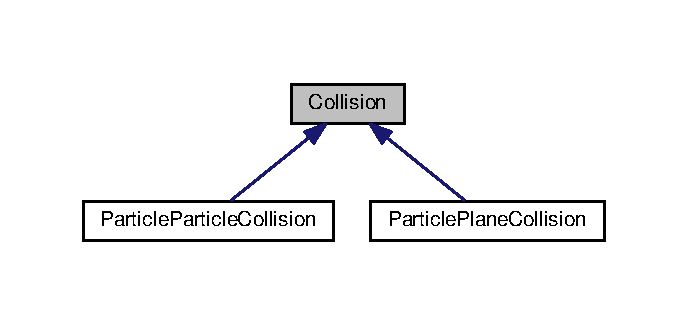
\includegraphics[width=330pt]{classCollision__inherit__graph}
\end{center}
\end{figure}
\subsection*{Public Member Functions}
\begin{DoxyCompactItemize}
\item 
virtual \hyperlink{classCollision_a81d1b669d7a8b03b178e794168ba7cec}{$\sim$\+Collision} ()
\item 
\hyperlink{classCollision_a62947cd726f639f2a30ad5deaa49ab71}{Collision} (float restitution)
\begin{DoxyCompactList}\small\item\em Build a collision event. \end{DoxyCompactList}\item 
void \hyperlink{classCollision_ad98c7014fd4237d0f0dcd159fdd24d1f}{solve\+Collision} ()
\begin{DoxyCompactList}\small\item\em Solve this collision. \end{DoxyCompactList}\end{DoxyCompactItemize}
\subsection*{Protected Attributes}
\begin{DoxyCompactItemize}
\item 
float \hyperlink{classCollision_a1158537ee89f6a5e1aab79f4ecd6a7d4}{m\+\_\+restitution}
\end{DoxyCompactItemize}
\subsection*{Private Member Functions}
\begin{DoxyCompactItemize}
\item 
virtual void \hyperlink{classCollision_a5fa2b29df51abd8723660cd07050e616}{do\+\_\+solve\+Collision} ()=0
\begin{DoxyCompactList}\small\item\em Implementation of the collision solving. \end{DoxyCompactList}\end{DoxyCompactItemize}


\subsection{Detailed Description}
This class store a collision event between two objects that should be resolved to avoid object inter-\/penetration. 

\subsection{Constructor \& Destructor Documentation}
\hypertarget{classCollision_a81d1b669d7a8b03b178e794168ba7cec}{\index{Collision@{Collision}!````~Collision@{$\sim$\+Collision}}
\index{````~Collision@{$\sim$\+Collision}!Collision@{Collision}}
\subsubsection[{$\sim$\+Collision}]{\setlength{\rightskip}{0pt plus 5cm}virtual Collision\+::$\sim$\+Collision (
\begin{DoxyParamCaption}
{}
\end{DoxyParamCaption}
)\hspace{0.3cm}{\ttfamily [virtual]}}}\label{classCollision_a81d1b669d7a8b03b178e794168ba7cec}
\hypertarget{classCollision_a62947cd726f639f2a30ad5deaa49ab71}{\index{Collision@{Collision}!Collision@{Collision}}
\index{Collision@{Collision}!Collision@{Collision}}
\subsubsection[{Collision}]{\setlength{\rightskip}{0pt plus 5cm}Collision\+::\+Collision (
\begin{DoxyParamCaption}
\item[{float}]{restitution}
\end{DoxyParamCaption}
)}}\label{classCollision_a62947cd726f639f2a30ad5deaa49ab71}
Build a collision event. 
\begin{DoxyParams}{Parameters}
{\em restitution} & Restitution factor of this collision. \\
\hline
\end{DoxyParams}


\subsection{Member Function Documentation}
\hypertarget{classCollision_a5fa2b29df51abd8723660cd07050e616}{\index{Collision@{Collision}!do\+\_\+solve\+Collision@{do\+\_\+solve\+Collision}}
\index{do\+\_\+solve\+Collision@{do\+\_\+solve\+Collision}!Collision@{Collision}}
\subsubsection[{do\+\_\+solve\+Collision}]{\setlength{\rightskip}{0pt plus 5cm}virtual void Collision\+::do\+\_\+solve\+Collision (
\begin{DoxyParamCaption}
{}
\end{DoxyParamCaption}
)\hspace{0.3cm}{\ttfamily [private]}, {\ttfamily [pure virtual]}}}\label{classCollision_a5fa2b29df51abd8723660cd07050e616}
Actual implementation of the collision solving, that should be done in derived classes. 

Implemented in \hyperlink{classParticlePlaneCollision_a1516ee9898275c1ad9bfbc8bad675b1b}{Particle\+Plane\+Collision}, and \hyperlink{classParticleParticleCollision_a9f18947965d8615faf1d957c259a65e2}{Particle\+Particle\+Collision}.

\hypertarget{classCollision_ad98c7014fd4237d0f0dcd159fdd24d1f}{\index{Collision@{Collision}!solve\+Collision@{solve\+Collision}}
\index{solve\+Collision@{solve\+Collision}!Collision@{Collision}}
\subsubsection[{solve\+Collision}]{\setlength{\rightskip}{0pt plus 5cm}void Collision\+::solve\+Collision (
\begin{DoxyParamCaption}
{}
\end{DoxyParamCaption}
)}}\label{classCollision_ad98c7014fd4237d0f0dcd159fdd24d1f}
Solve this collision to update the positions and velocities of objects that collided. 

\subsection{Member Data Documentation}
\hypertarget{classCollision_a1158537ee89f6a5e1aab79f4ecd6a7d4}{\index{Collision@{Collision}!m\+\_\+restitution@{m\+\_\+restitution}}
\index{m\+\_\+restitution@{m\+\_\+restitution}!Collision@{Collision}}
\subsubsection[{m\+\_\+restitution}]{\setlength{\rightskip}{0pt plus 5cm}float Collision\+::m\+\_\+restitution\hspace{0.3cm}{\ttfamily [protected]}}}\label{classCollision_a1158537ee89f6a5e1aab79f4ecd6a7d4}


The documentation for this class was generated from the following file\+:\begin{DoxyCompactItemize}
\item 
/home/chardon/\+Depot/ensimag/2\+A\+\_\+\+G3\+D/practicals/teacher\+Source/include/dynamics/\hyperlink{Collision_8hpp}{Collision.\+hpp}\end{DoxyCompactItemize}

\hypertarget{classConstantForceField}{\section{Constant\+Force\+Field Class Reference}
\label{classConstantForceField}\index{Constant\+Force\+Field@{Constant\+Force\+Field}}
}


Constant force field.  




{\ttfamily \#include $<$Constant\+Force\+Field.\+hpp$>$}



Inheritance diagram for Constant\+Force\+Field\+:\nopagebreak
\begin{figure}[H]
\begin{center}
\leavevmode
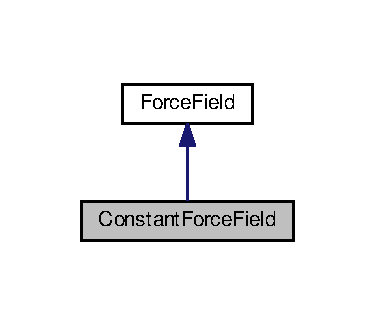
\includegraphics[width=180pt]{classConstantForceField__inherit__graph}
\end{center}
\end{figure}


Collaboration diagram for Constant\+Force\+Field\+:\nopagebreak
\begin{figure}[H]
\begin{center}
\leavevmode
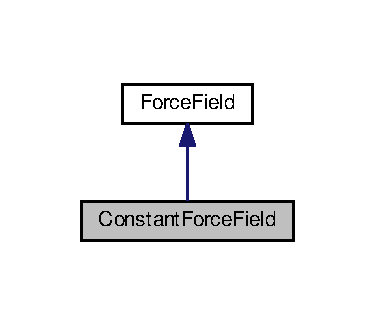
\includegraphics[width=180pt]{classConstantForceField__coll__graph}
\end{center}
\end{figure}
\subsection*{Public Member Functions}
\begin{DoxyCompactItemize}
\item 
\hyperlink{classConstantForceField_aae2c264a31c790130fc0b76c6e93160b}{Constant\+Force\+Field} (const std\+::vector$<$ \hyperlink{Particle_8hpp_a9a7abc8635002993537b61ef2c857fdd}{Particle\+Ptr} $>$ \&particles, const glm\+::vec3 \&force)
\begin{DoxyCompactList}\small\item\em Build a constant force field. \end{DoxyCompactList}\item 
const std\+::vector$<$ \hyperlink{Particle_8hpp_a9a7abc8635002993537b61ef2c857fdd}{Particle\+Ptr} $>$ \hyperlink{classConstantForceField_a80d7579494fc32b0c83daab452130371}{get\+Particles} ()
\begin{DoxyCompactList}\small\item\em Access to the set of managed particles. \end{DoxyCompactList}\item 
void \hyperlink{classConstantForceField_acd6c41391f38bb37890a7a9f5864e04d}{set\+Particles} (const std\+::vector$<$ \hyperlink{Particle_8hpp_a9a7abc8635002993537b61ef2c857fdd}{Particle\+Ptr} $>$ \&particles)
\begin{DoxyCompactList}\small\item\em Define a new set of particles managed by this constant force field. \end{DoxyCompactList}\item 
const glm\+::vec3 \& \hyperlink{classConstantForceField_a7e914a757101de443694df79f9665586}{get\+Force} ()
\begin{DoxyCompactList}\small\item\em Access to the force applied to all influenced particles. \end{DoxyCompactList}\item 
void \hyperlink{classConstantForceField_a46c997f9f771cc83ef47bfdf6898734a}{set\+Force} (const glm\+::vec3 \&force)
\begin{DoxyCompactList}\small\item\em Set the force applied to all influenced particles. \end{DoxyCompactList}\end{DoxyCompactItemize}
\subsection*{Private Member Functions}
\begin{DoxyCompactItemize}
\item 
void \hyperlink{classConstantForceField_a4336bdbfa85ac10cc8a50170ab515061}{do\+\_\+add\+Force} ()
\begin{DoxyCompactList}\small\item\em Add force implementation. \end{DoxyCompactList}\end{DoxyCompactItemize}
\subsection*{Private Attributes}
\begin{DoxyCompactItemize}
\item 
std\+::vector$<$ \hyperlink{Particle_8hpp_a9a7abc8635002993537b61ef2c857fdd}{Particle\+Ptr} $>$ \hyperlink{classConstantForceField_acedcc9ed06f8d7b10714db6c321a188d}{m\+\_\+particles}
\item 
glm\+::vec3 \hyperlink{classConstantForceField_abba1f35001942ccdb89cb9a8a654d373}{m\+\_\+force}
\end{DoxyCompactItemize}


\subsection{Detailed Description}
Implementation of a force field that is constant, i.\+e. the same for all managed particles. 

\subsection{Constructor \& Destructor Documentation}
\hypertarget{classConstantForceField_aae2c264a31c790130fc0b76c6e93160b}{\index{Constant\+Force\+Field@{Constant\+Force\+Field}!Constant\+Force\+Field@{Constant\+Force\+Field}}
\index{Constant\+Force\+Field@{Constant\+Force\+Field}!Constant\+Force\+Field@{Constant\+Force\+Field}}
\subsubsection[{Constant\+Force\+Field}]{\setlength{\rightskip}{0pt plus 5cm}Constant\+Force\+Field\+::\+Constant\+Force\+Field (
\begin{DoxyParamCaption}
\item[{const std\+::vector$<$ {\bf Particle\+Ptr} $>$ \&}]{particles, }
\item[{const glm\+::vec3 \&}]{force}
\end{DoxyParamCaption}
)}}\label{classConstantForceField_aae2c264a31c790130fc0b76c6e93160b}
Build a constant force field for a set of particles. 
\begin{DoxyParams}{Parameters}
{\em particles} & The set of particles influenced by this force field. \\
\hline
{\em force} & The constant force applied to all particles. \\
\hline
\end{DoxyParams}


\subsection{Member Function Documentation}
\hypertarget{classConstantForceField_a4336bdbfa85ac10cc8a50170ab515061}{\index{Constant\+Force\+Field@{Constant\+Force\+Field}!do\+\_\+add\+Force@{do\+\_\+add\+Force}}
\index{do\+\_\+add\+Force@{do\+\_\+add\+Force}!Constant\+Force\+Field@{Constant\+Force\+Field}}
\subsubsection[{do\+\_\+add\+Force}]{\setlength{\rightskip}{0pt plus 5cm}void Constant\+Force\+Field\+::do\+\_\+add\+Force (
\begin{DoxyParamCaption}
{}
\end{DoxyParamCaption}
)\hspace{0.3cm}{\ttfamily [private]}, {\ttfamily [virtual]}}}\label{classConstantForceField_a4336bdbfa85ac10cc8a50170ab515061}
The actual implementation to add force to the particles. This should be implemented in derived classes. 

Implements \hyperlink{classForceField_a2f44520a00188a3aaeb04e667e8d2673}{Force\+Field}.

\hypertarget{classConstantForceField_a7e914a757101de443694df79f9665586}{\index{Constant\+Force\+Field@{Constant\+Force\+Field}!get\+Force@{get\+Force}}
\index{get\+Force@{get\+Force}!Constant\+Force\+Field@{Constant\+Force\+Field}}
\subsubsection[{get\+Force}]{\setlength{\rightskip}{0pt plus 5cm}const glm\+::vec3\& Constant\+Force\+Field\+::get\+Force (
\begin{DoxyParamCaption}
{}
\end{DoxyParamCaption}
)}}\label{classConstantForceField_a7e914a757101de443694df79f9665586}
Get the constant force of this force field. \begin{DoxyReturn}{Returns}
The force of this force field. 
\end{DoxyReturn}
\hypertarget{classConstantForceField_a80d7579494fc32b0c83daab452130371}{\index{Constant\+Force\+Field@{Constant\+Force\+Field}!get\+Particles@{get\+Particles}}
\index{get\+Particles@{get\+Particles}!Constant\+Force\+Field@{Constant\+Force\+Field}}
\subsubsection[{get\+Particles}]{\setlength{\rightskip}{0pt plus 5cm}const std\+::vector$<${\bf Particle\+Ptr}$>$ Constant\+Force\+Field\+::get\+Particles (
\begin{DoxyParamCaption}
{}
\end{DoxyParamCaption}
)}}\label{classConstantForceField_a80d7579494fc32b0c83daab452130371}
Get the set of managed particles of this constant force field. \begin{DoxyReturn}{Returns}
The managed force field. 
\end{DoxyReturn}
\hypertarget{classConstantForceField_a46c997f9f771cc83ef47bfdf6898734a}{\index{Constant\+Force\+Field@{Constant\+Force\+Field}!set\+Force@{set\+Force}}
\index{set\+Force@{set\+Force}!Constant\+Force\+Field@{Constant\+Force\+Field}}
\subsubsection[{set\+Force}]{\setlength{\rightskip}{0pt plus 5cm}void Constant\+Force\+Field\+::set\+Force (
\begin{DoxyParamCaption}
\item[{const glm\+::vec3 \&}]{force}
\end{DoxyParamCaption}
)}}\label{classConstantForceField_a46c997f9f771cc83ef47bfdf6898734a}
Set the force applied to all particles influenced by this force field. 
\begin{DoxyParams}{Parameters}
{\em force} & The new force. \\
\hline
\end{DoxyParams}
\hypertarget{classConstantForceField_acd6c41391f38bb37890a7a9f5864e04d}{\index{Constant\+Force\+Field@{Constant\+Force\+Field}!set\+Particles@{set\+Particles}}
\index{set\+Particles@{set\+Particles}!Constant\+Force\+Field@{Constant\+Force\+Field}}
\subsubsection[{set\+Particles}]{\setlength{\rightskip}{0pt plus 5cm}void Constant\+Force\+Field\+::set\+Particles (
\begin{DoxyParamCaption}
\item[{const std\+::vector$<$ {\bf Particle\+Ptr} $>$ \&}]{particles}
\end{DoxyParamCaption}
)}}\label{classConstantForceField_acd6c41391f38bb37890a7a9f5864e04d}
Set the particles influenced by this constant force field. 
\begin{DoxyParams}{Parameters}
{\em particles} & The new set of particles. \\
\hline
\end{DoxyParams}


\subsection{Member Data Documentation}
\hypertarget{classConstantForceField_abba1f35001942ccdb89cb9a8a654d373}{\index{Constant\+Force\+Field@{Constant\+Force\+Field}!m\+\_\+force@{m\+\_\+force}}
\index{m\+\_\+force@{m\+\_\+force}!Constant\+Force\+Field@{Constant\+Force\+Field}}
\subsubsection[{m\+\_\+force}]{\setlength{\rightskip}{0pt plus 5cm}glm\+::vec3 Constant\+Force\+Field\+::m\+\_\+force\hspace{0.3cm}{\ttfamily [private]}}}\label{classConstantForceField_abba1f35001942ccdb89cb9a8a654d373}
\hypertarget{classConstantForceField_acedcc9ed06f8d7b10714db6c321a188d}{\index{Constant\+Force\+Field@{Constant\+Force\+Field}!m\+\_\+particles@{m\+\_\+particles}}
\index{m\+\_\+particles@{m\+\_\+particles}!Constant\+Force\+Field@{Constant\+Force\+Field}}
\subsubsection[{m\+\_\+particles}]{\setlength{\rightskip}{0pt plus 5cm}std\+::vector$<${\bf Particle\+Ptr}$>$ Constant\+Force\+Field\+::m\+\_\+particles\hspace{0.3cm}{\ttfamily [private]}}}\label{classConstantForceField_acedcc9ed06f8d7b10714db6c321a188d}


The documentation for this class was generated from the following file\+:\begin{DoxyCompactItemize}
\item 
/home/chardon/\+Depot/ensimag/2\+A\+\_\+\+G3\+D/practicals/teacher\+Source/include/dynamics/\hyperlink{ConstantForceField_8hpp}{Constant\+Force\+Field.\+hpp}\end{DoxyCompactItemize}

\hypertarget{classConstantForceFieldRenderable}{\section{Constant\+Force\+Field\+Renderable Class Reference}
\label{classConstantForceFieldRenderable}\index{Constant\+Force\+Field\+Renderable@{Constant\+Force\+Field\+Renderable}}
}


Render a constant force field.  




{\ttfamily \#include $<$Constant\+Force\+Field\+Renderable.\+hpp$>$}



Inheritance diagram for Constant\+Force\+Field\+Renderable\+:\nopagebreak
\begin{figure}[H]
\begin{center}
\leavevmode
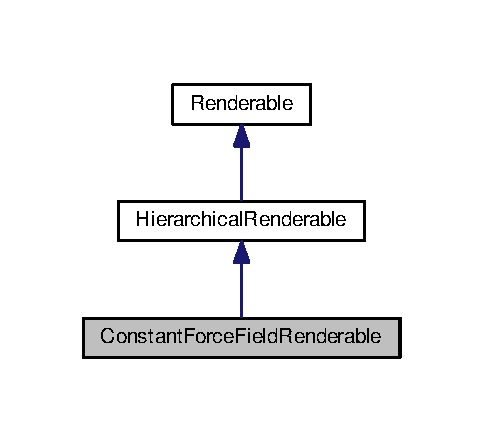
\includegraphics[width=232pt]{classConstantForceFieldRenderable__inherit__graph}
\end{center}
\end{figure}


Collaboration diagram for Constant\+Force\+Field\+Renderable\+:\nopagebreak
\begin{figure}[H]
\begin{center}
\leavevmode
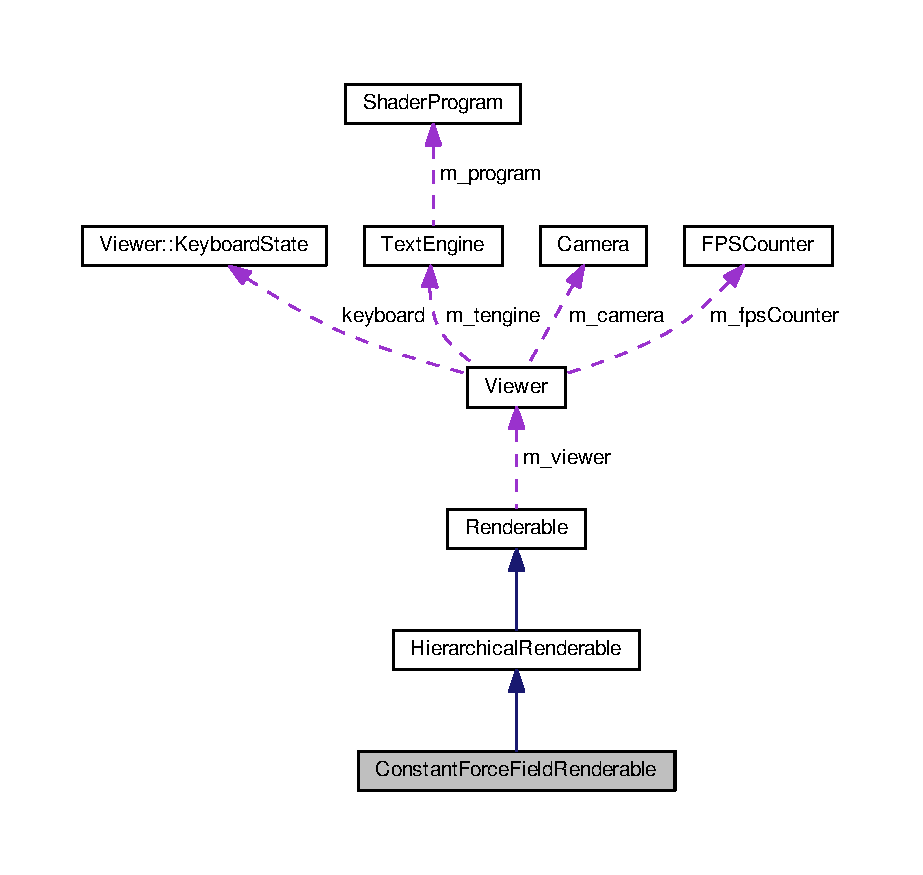
\includegraphics[width=350pt]{classConstantForceFieldRenderable__coll__graph}
\end{center}
\end{figure}
\subsection*{Public Member Functions}
\begin{DoxyCompactItemize}
\item 
\hyperlink{classConstantForceFieldRenderable_a5b3b26ab2ddb497413df242773f941a2}{$\sim$\+Constant\+Force\+Field\+Renderable} ()
\item 
\hyperlink{classConstantForceFieldRenderable_a47f65f935336c605e55d94efb84e6842}{Constant\+Force\+Field\+Renderable} (\hyperlink{ShaderProgram_8hpp_af8e4af1ad4c53875ee5d32ab7e1f4966}{Shader\+Program\+Ptr} program, \hyperlink{ConstantForceField_8hpp_a7b80b566be4aeb0b5474a8aeb2e0ff49}{Constant\+Force\+Field\+Ptr} force\+Field)
\begin{DoxyCompactList}\small\item\em Build a renderable for a constant force field. \end{DoxyCompactList}\end{DoxyCompactItemize}
\subsection*{Private Member Functions}
\begin{DoxyCompactItemize}
\item 
void \hyperlink{classConstantForceFieldRenderable_af9ee973e392967a5da31b0b9b67d3fdd}{do\+\_\+draw} ()
\begin{DoxyCompactList}\small\item\em Draw virtual function. \end{DoxyCompactList}\item 
void \hyperlink{classConstantForceFieldRenderable_aa2c53dcf6411244d5a5e4ed562f9574c}{do\+\_\+animate} (float time)
\begin{DoxyCompactList}\small\item\em Animate virtual function. \end{DoxyCompactList}\end{DoxyCompactItemize}
\subsection*{Private Attributes}
\begin{DoxyCompactItemize}
\item 
\hyperlink{ConstantForceField_8hpp_a7b80b566be4aeb0b5474a8aeb2e0ff49}{Constant\+Force\+Field\+Ptr} \hyperlink{classConstantForceFieldRenderable_ac9613a4d0ca11522749d2416b51cf1c5}{m\+\_\+force\+Field}
\item 
std\+::vector$<$ glm\+::vec3 $>$ \hyperlink{classConstantForceFieldRenderable_adda5c978538c39f9ce237bc4914d0399}{m\+\_\+positions}
\item 
std\+::vector$<$ glm\+::vec4 $>$ \hyperlink{classConstantForceFieldRenderable_a78a6bde3ae426f7367563718573ef9e3}{m\+\_\+colors}
\item 
std\+::vector$<$ glm\+::vec3 $>$ \hyperlink{classConstantForceFieldRenderable_a171dc24ba94fd9337d36758e8791cebb}{m\+\_\+normals}
\item 
unsigned int \hyperlink{classConstantForceFieldRenderable_a170f25325d424be2a1533befc64b1648}{m\+\_\+p\+Buffer}
\item 
unsigned int \hyperlink{classConstantForceFieldRenderable_a6c7501e6c02b7c49b7ee253563000eff}{m\+\_\+c\+Buffer}
\item 
unsigned int \hyperlink{classConstantForceFieldRenderable_af160da689aab9e5b38558cc159f9f2e4}{m\+\_\+n\+Buffer}
\end{DoxyCompactItemize}
\subsection*{Additional Inherited Members}


\subsection{Detailed Description}
This class is used to render a constant force field. 

\subsection{Constructor \& Destructor Documentation}
\hypertarget{classConstantForceFieldRenderable_a5b3b26ab2ddb497413df242773f941a2}{\index{Constant\+Force\+Field\+Renderable@{Constant\+Force\+Field\+Renderable}!````~Constant\+Force\+Field\+Renderable@{$\sim$\+Constant\+Force\+Field\+Renderable}}
\index{````~Constant\+Force\+Field\+Renderable@{$\sim$\+Constant\+Force\+Field\+Renderable}!Constant\+Force\+Field\+Renderable@{Constant\+Force\+Field\+Renderable}}
\subsubsection[{$\sim$\+Constant\+Force\+Field\+Renderable}]{\setlength{\rightskip}{0pt plus 5cm}Constant\+Force\+Field\+Renderable\+::$\sim$\+Constant\+Force\+Field\+Renderable (
\begin{DoxyParamCaption}
{}
\end{DoxyParamCaption}
)}}\label{classConstantForceFieldRenderable_a5b3b26ab2ddb497413df242773f941a2}
\hypertarget{classConstantForceFieldRenderable_a47f65f935336c605e55d94efb84e6842}{\index{Constant\+Force\+Field\+Renderable@{Constant\+Force\+Field\+Renderable}!Constant\+Force\+Field\+Renderable@{Constant\+Force\+Field\+Renderable}}
\index{Constant\+Force\+Field\+Renderable@{Constant\+Force\+Field\+Renderable}!Constant\+Force\+Field\+Renderable@{Constant\+Force\+Field\+Renderable}}
\subsubsection[{Constant\+Force\+Field\+Renderable}]{\setlength{\rightskip}{0pt plus 5cm}Constant\+Force\+Field\+Renderable\+::\+Constant\+Force\+Field\+Renderable (
\begin{DoxyParamCaption}
\item[{{\bf Shader\+Program\+Ptr}}]{program, }
\item[{{\bf Constant\+Force\+Field\+Ptr}}]{force\+Field}
\end{DoxyParamCaption}
)}}\label{classConstantForceFieldRenderable_a47f65f935336c605e55d94efb84e6842}
Create a renderable for a constant force field. 
\begin{DoxyParams}{Parameters}
{\em program} & Shader program to use to render the constant force field. \\
\hline
{\em force\+Field} & The constant force field to render. \\
\hline
\end{DoxyParams}


\subsection{Member Function Documentation}
\hypertarget{classConstantForceFieldRenderable_aa2c53dcf6411244d5a5e4ed562f9574c}{\index{Constant\+Force\+Field\+Renderable@{Constant\+Force\+Field\+Renderable}!do\+\_\+animate@{do\+\_\+animate}}
\index{do\+\_\+animate@{do\+\_\+animate}!Constant\+Force\+Field\+Renderable@{Constant\+Force\+Field\+Renderable}}
\subsubsection[{do\+\_\+animate}]{\setlength{\rightskip}{0pt plus 5cm}void Constant\+Force\+Field\+Renderable\+::do\+\_\+animate (
\begin{DoxyParamCaption}
\item[{float}]{time}
\end{DoxyParamCaption}
)\hspace{0.3cm}{\ttfamily [private]}, {\ttfamily [virtual]}}}\label{classConstantForceFieldRenderable_aa2c53dcf6411244d5a5e4ed562f9574c}
Implementation to animate this renderable. 
\begin{DoxyParams}{Parameters}
{\em time} & The current simulation time. \\
\hline
\end{DoxyParams}


Implements \hyperlink{classRenderable_aa5206322555c9dece40b21e797629b34}{Renderable}.

\hypertarget{classConstantForceFieldRenderable_af9ee973e392967a5da31b0b9b67d3fdd}{\index{Constant\+Force\+Field\+Renderable@{Constant\+Force\+Field\+Renderable}!do\+\_\+draw@{do\+\_\+draw}}
\index{do\+\_\+draw@{do\+\_\+draw}!Constant\+Force\+Field\+Renderable@{Constant\+Force\+Field\+Renderable}}
\subsubsection[{do\+\_\+draw}]{\setlength{\rightskip}{0pt plus 5cm}void Constant\+Force\+Field\+Renderable\+::do\+\_\+draw (
\begin{DoxyParamCaption}
{}
\end{DoxyParamCaption}
)\hspace{0.3cm}{\ttfamily [private]}, {\ttfamily [virtual]}}}\label{classConstantForceFieldRenderable_af9ee973e392967a5da31b0b9b67d3fdd}
Implementation to draw this renderable. 

Implements \hyperlink{classRenderable_a98ab6308c1d2b56dacda7c435fb38d5b}{Renderable}.



\subsection{Member Data Documentation}
\hypertarget{classConstantForceFieldRenderable_a6c7501e6c02b7c49b7ee253563000eff}{\index{Constant\+Force\+Field\+Renderable@{Constant\+Force\+Field\+Renderable}!m\+\_\+c\+Buffer@{m\+\_\+c\+Buffer}}
\index{m\+\_\+c\+Buffer@{m\+\_\+c\+Buffer}!Constant\+Force\+Field\+Renderable@{Constant\+Force\+Field\+Renderable}}
\subsubsection[{m\+\_\+c\+Buffer}]{\setlength{\rightskip}{0pt plus 5cm}unsigned int Constant\+Force\+Field\+Renderable\+::m\+\_\+c\+Buffer\hspace{0.3cm}{\ttfamily [private]}}}\label{classConstantForceFieldRenderable_a6c7501e6c02b7c49b7ee253563000eff}
\hypertarget{classConstantForceFieldRenderable_a78a6bde3ae426f7367563718573ef9e3}{\index{Constant\+Force\+Field\+Renderable@{Constant\+Force\+Field\+Renderable}!m\+\_\+colors@{m\+\_\+colors}}
\index{m\+\_\+colors@{m\+\_\+colors}!Constant\+Force\+Field\+Renderable@{Constant\+Force\+Field\+Renderable}}
\subsubsection[{m\+\_\+colors}]{\setlength{\rightskip}{0pt plus 5cm}std\+::vector$<$ glm\+::vec4 $>$ Constant\+Force\+Field\+Renderable\+::m\+\_\+colors\hspace{0.3cm}{\ttfamily [private]}}}\label{classConstantForceFieldRenderable_a78a6bde3ae426f7367563718573ef9e3}
\hypertarget{classConstantForceFieldRenderable_ac9613a4d0ca11522749d2416b51cf1c5}{\index{Constant\+Force\+Field\+Renderable@{Constant\+Force\+Field\+Renderable}!m\+\_\+force\+Field@{m\+\_\+force\+Field}}
\index{m\+\_\+force\+Field@{m\+\_\+force\+Field}!Constant\+Force\+Field\+Renderable@{Constant\+Force\+Field\+Renderable}}
\subsubsection[{m\+\_\+force\+Field}]{\setlength{\rightskip}{0pt plus 5cm}{\bf Constant\+Force\+Field\+Ptr} Constant\+Force\+Field\+Renderable\+::m\+\_\+force\+Field\hspace{0.3cm}{\ttfamily [private]}}}\label{classConstantForceFieldRenderable_ac9613a4d0ca11522749d2416b51cf1c5}
\hypertarget{classConstantForceFieldRenderable_af160da689aab9e5b38558cc159f9f2e4}{\index{Constant\+Force\+Field\+Renderable@{Constant\+Force\+Field\+Renderable}!m\+\_\+n\+Buffer@{m\+\_\+n\+Buffer}}
\index{m\+\_\+n\+Buffer@{m\+\_\+n\+Buffer}!Constant\+Force\+Field\+Renderable@{Constant\+Force\+Field\+Renderable}}
\subsubsection[{m\+\_\+n\+Buffer}]{\setlength{\rightskip}{0pt plus 5cm}unsigned int Constant\+Force\+Field\+Renderable\+::m\+\_\+n\+Buffer\hspace{0.3cm}{\ttfamily [private]}}}\label{classConstantForceFieldRenderable_af160da689aab9e5b38558cc159f9f2e4}
\hypertarget{classConstantForceFieldRenderable_a171dc24ba94fd9337d36758e8791cebb}{\index{Constant\+Force\+Field\+Renderable@{Constant\+Force\+Field\+Renderable}!m\+\_\+normals@{m\+\_\+normals}}
\index{m\+\_\+normals@{m\+\_\+normals}!Constant\+Force\+Field\+Renderable@{Constant\+Force\+Field\+Renderable}}
\subsubsection[{m\+\_\+normals}]{\setlength{\rightskip}{0pt plus 5cm}std\+::vector$<$ glm\+::vec3 $>$ Constant\+Force\+Field\+Renderable\+::m\+\_\+normals\hspace{0.3cm}{\ttfamily [private]}}}\label{classConstantForceFieldRenderable_a171dc24ba94fd9337d36758e8791cebb}
\hypertarget{classConstantForceFieldRenderable_a170f25325d424be2a1533befc64b1648}{\index{Constant\+Force\+Field\+Renderable@{Constant\+Force\+Field\+Renderable}!m\+\_\+p\+Buffer@{m\+\_\+p\+Buffer}}
\index{m\+\_\+p\+Buffer@{m\+\_\+p\+Buffer}!Constant\+Force\+Field\+Renderable@{Constant\+Force\+Field\+Renderable}}
\subsubsection[{m\+\_\+p\+Buffer}]{\setlength{\rightskip}{0pt plus 5cm}unsigned int Constant\+Force\+Field\+Renderable\+::m\+\_\+p\+Buffer\hspace{0.3cm}{\ttfamily [private]}}}\label{classConstantForceFieldRenderable_a170f25325d424be2a1533befc64b1648}
\hypertarget{classConstantForceFieldRenderable_adda5c978538c39f9ce237bc4914d0399}{\index{Constant\+Force\+Field\+Renderable@{Constant\+Force\+Field\+Renderable}!m\+\_\+positions@{m\+\_\+positions}}
\index{m\+\_\+positions@{m\+\_\+positions}!Constant\+Force\+Field\+Renderable@{Constant\+Force\+Field\+Renderable}}
\subsubsection[{m\+\_\+positions}]{\setlength{\rightskip}{0pt plus 5cm}std\+::vector$<$ glm\+::vec3 $>$ Constant\+Force\+Field\+Renderable\+::m\+\_\+positions\hspace{0.3cm}{\ttfamily [private]}}}\label{classConstantForceFieldRenderable_adda5c978538c39f9ce237bc4914d0399}


The documentation for this class was generated from the following file\+:\begin{DoxyCompactItemize}
\item 
/home/chardon/\+Depot/ensimag/2\+A\+\_\+\+G3\+D/practicals/teacher\+Source/include/dynamics/\hyperlink{ConstantForceFieldRenderable_8hpp}{Constant\+Force\+Field\+Renderable.\+hpp}\end{DoxyCompactItemize}

\hypertarget{classControlledForceFieldRenderable}{\section{Controlled\+Force\+Field\+Renderable Class Reference}
\label{classControlledForceFieldRenderable}\index{Controlled\+Force\+Field\+Renderable@{Controlled\+Force\+Field\+Renderable}}
}


Implement a force field controlled by user input.  




{\ttfamily \#include $<$Controlled\+Force\+Field\+Renderable.\+hpp$>$}



Inheritance diagram for Controlled\+Force\+Field\+Renderable\+:\nopagebreak
\begin{figure}[H]
\begin{center}
\leavevmode
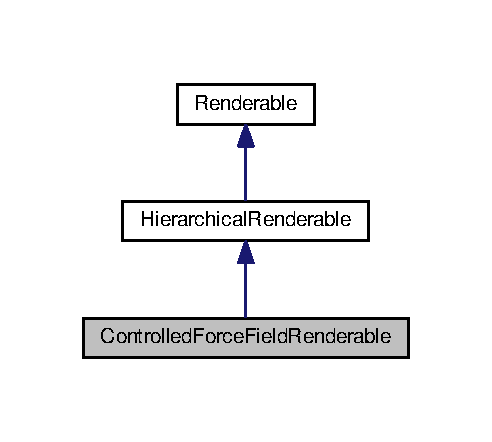
\includegraphics[width=236pt]{classControlledForceFieldRenderable__inherit__graph}
\end{center}
\end{figure}


Collaboration diagram for Controlled\+Force\+Field\+Renderable\+:\nopagebreak
\begin{figure}[H]
\begin{center}
\leavevmode
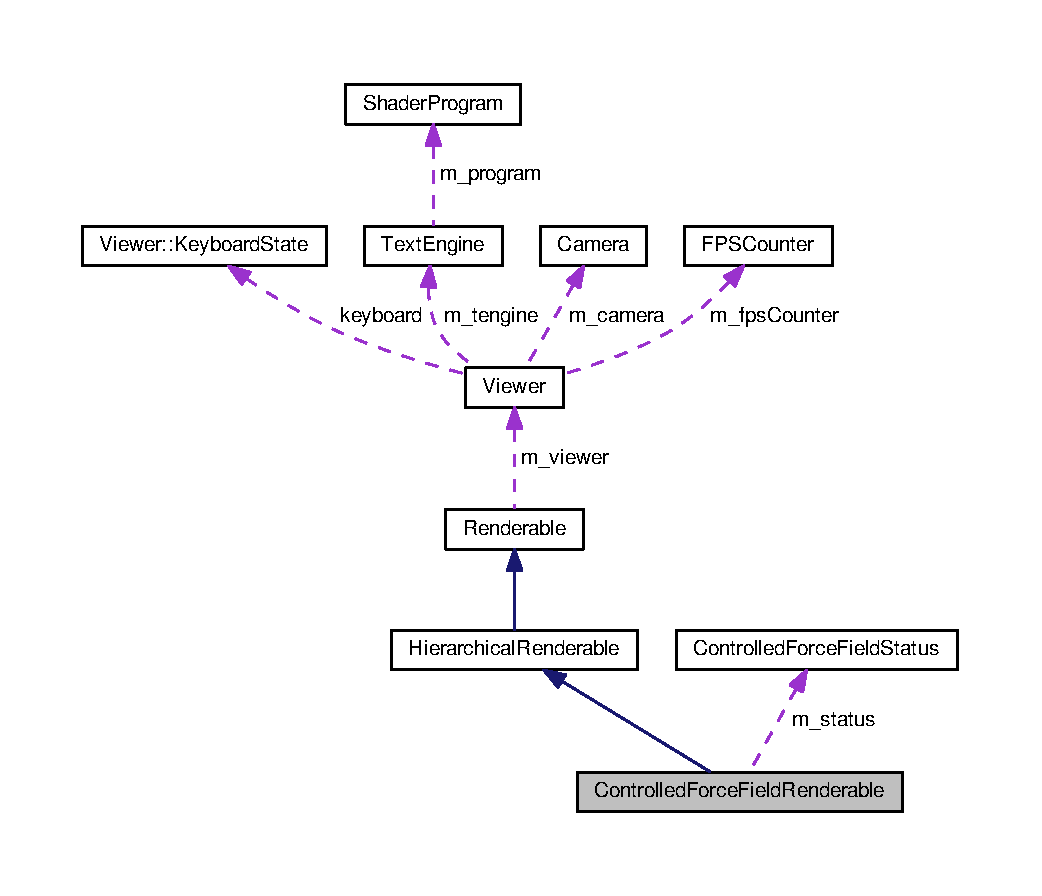
\includegraphics[width=350pt]{classControlledForceFieldRenderable__coll__graph}
\end{center}
\end{figure}
\subsection*{Public Member Functions}
\begin{DoxyCompactItemize}
\item 
\hyperlink{classControlledForceFieldRenderable_a0b3f0aa9e5b4eca0146beefd5ba8862f}{Controlled\+Force\+Field\+Renderable} (\hyperlink{ShaderProgram_8hpp_af8e4af1ad4c53875ee5d32ab7e1f4966}{Shader\+Program\+Ptr} program, \hyperlink{ConstantForceField_8hpp_a7b80b566be4aeb0b5474a8aeb2e0ff49}{Constant\+Force\+Field\+Ptr} force\+Field)
\begin{DoxyCompactList}\small\item\em Build a new controlled force field renderable. \end{DoxyCompactList}\item 
\hyperlink{classControlledForceFieldRenderable_ad5dff1b4ecdbda434729e8a4ef68073a}{$\sim$\+Controlled\+Force\+Field\+Renderable} ()
\end{DoxyCompactItemize}
\subsection*{Private Member Functions}
\begin{DoxyCompactItemize}
\item 
virtual void \hyperlink{classControlledForceFieldRenderable_a7313ffabf0b3d4bf27c10d57d7f143de}{do\+\_\+key\+Pressed\+Event} (sf\+::\+Event \&e)
\begin{DoxyCompactList}\small\item\em Handle a key pressed event. \end{DoxyCompactList}\item 
virtual void \hyperlink{classControlledForceFieldRenderable_a68aaf096b1bf911717c9374abc51e3df}{do\+\_\+key\+Released\+Event} (sf\+::\+Event \&e)
\begin{DoxyCompactList}\small\item\em Handle a key released event. \end{DoxyCompactList}\item 
virtual void \hyperlink{classControlledForceFieldRenderable_a3ab6b5efaa5d5b988d92c4fee3e770a0}{do\+\_\+animate} (float time)
\begin{DoxyCompactList}\small\item\em Animate virtual function. \end{DoxyCompactList}\item 
virtual void \hyperlink{classControlledForceFieldRenderable_a5b73eb28c70b0a37ce4f69ec6a63823a}{do\+\_\+draw} ()
\begin{DoxyCompactList}\small\item\em Draw virtual function. \end{DoxyCompactList}\end{DoxyCompactItemize}
\subsection*{Private Attributes}
\begin{DoxyCompactItemize}
\item 
\hyperlink{classControlledForceFieldStatus}{Controlled\+Force\+Field\+Status} \hyperlink{classControlledForceFieldRenderable_aeb5e06ce7914d6050578f9466d3c67ad}{m\+\_\+status}
\item 
\hyperlink{ConstantForceField_8hpp_a7b80b566be4aeb0b5474a8aeb2e0ff49}{Constant\+Force\+Field\+Ptr} \hyperlink{classControlledForceFieldRenderable_a6832a057549138e1f7aea221677be189}{m\+\_\+force}
\item 
std\+::vector$<$ glm\+::vec3 $>$ \hyperlink{classControlledForceFieldRenderable_a754e3c8fe79f1d95020f631fae8a6e40}{m\+\_\+positions}
\item 
std\+::vector$<$ glm\+::vec4 $>$ \hyperlink{classControlledForceFieldRenderable_a825c0d5323c7bc212b4b9325614a9414}{m\+\_\+colors}
\item 
std\+::vector$<$ glm\+::vec3 $>$ \hyperlink{classControlledForceFieldRenderable_ab6d76f2f8b7ea00b0facdc0938808a25}{m\+\_\+normals}
\item 
unsigned int \hyperlink{classControlledForceFieldRenderable_a53bfe9b2180551039b1c7eb54f2d4974}{m\+\_\+p\+Buffer}
\item 
unsigned int \hyperlink{classControlledForceFieldRenderable_a7494339c295c2b0b6550e34c89fbd9c1}{m\+\_\+c\+Buffer}
\item 
unsigned int \hyperlink{classControlledForceFieldRenderable_a314a07bcaed1f7db3ded7283996474c3}{m\+\_\+n\+Buffer}
\end{DoxyCompactItemize}
\subsection*{Additional Inherited Members}


\subsection{Detailed Description}
This class is an example of what you could do to control a dynamic component (e.\+g. the kart in your project) thanks to user inputs. This is done by modifying the force of a constant force field applied to the mobile(s) you want to control.

We derive from a renderable to be able to react to user input. This might look nasty, but since you dealt with renderables during all previous praticales, we think this is the easiest way to do so. We derive from a hierarchical renderable to be able to use the same local frame as the dynamic system using the force field (see \hyperlink{classDynamicSystemRenderable}{Dynamic\+System\+Renderable}). 

\subsection{Constructor \& Destructor Documentation}
\hypertarget{classControlledForceFieldRenderable_a0b3f0aa9e5b4eca0146beefd5ba8862f}{\index{Controlled\+Force\+Field\+Renderable@{Controlled\+Force\+Field\+Renderable}!Controlled\+Force\+Field\+Renderable@{Controlled\+Force\+Field\+Renderable}}
\index{Controlled\+Force\+Field\+Renderable@{Controlled\+Force\+Field\+Renderable}!Controlled\+Force\+Field\+Renderable@{Controlled\+Force\+Field\+Renderable}}
\subsubsection[{Controlled\+Force\+Field\+Renderable}]{\setlength{\rightskip}{0pt plus 5cm}Controlled\+Force\+Field\+Renderable\+::\+Controlled\+Force\+Field\+Renderable (
\begin{DoxyParamCaption}
\item[{{\bf Shader\+Program\+Ptr}}]{program, }
\item[{{\bf Constant\+Force\+Field\+Ptr}}]{force\+Field}
\end{DoxyParamCaption}
)}}\label{classControlledForceFieldRenderable_a0b3f0aa9e5b4eca0146beefd5ba8862f}
Build a new controlled force field by user inputs. 
\begin{DoxyParams}{Parameters}
{\em program} & The shader program used to render the force applied to particles. \\
\hline
{\em force\+Field} & The force field to control with user inputs. \\
\hline
\end{DoxyParams}
\hypertarget{classControlledForceFieldRenderable_ad5dff1b4ecdbda434729e8a4ef68073a}{\index{Controlled\+Force\+Field\+Renderable@{Controlled\+Force\+Field\+Renderable}!````~Controlled\+Force\+Field\+Renderable@{$\sim$\+Controlled\+Force\+Field\+Renderable}}
\index{````~Controlled\+Force\+Field\+Renderable@{$\sim$\+Controlled\+Force\+Field\+Renderable}!Controlled\+Force\+Field\+Renderable@{Controlled\+Force\+Field\+Renderable}}
\subsubsection[{$\sim$\+Controlled\+Force\+Field\+Renderable}]{\setlength{\rightskip}{0pt plus 5cm}Controlled\+Force\+Field\+Renderable\+::$\sim$\+Controlled\+Force\+Field\+Renderable (
\begin{DoxyParamCaption}
{}
\end{DoxyParamCaption}
)}}\label{classControlledForceFieldRenderable_ad5dff1b4ecdbda434729e8a4ef68073a}


\subsection{Member Function Documentation}
\hypertarget{classControlledForceFieldRenderable_a3ab6b5efaa5d5b988d92c4fee3e770a0}{\index{Controlled\+Force\+Field\+Renderable@{Controlled\+Force\+Field\+Renderable}!do\+\_\+animate@{do\+\_\+animate}}
\index{do\+\_\+animate@{do\+\_\+animate}!Controlled\+Force\+Field\+Renderable@{Controlled\+Force\+Field\+Renderable}}
\subsubsection[{do\+\_\+animate}]{\setlength{\rightskip}{0pt plus 5cm}virtual void Controlled\+Force\+Field\+Renderable\+::do\+\_\+animate (
\begin{DoxyParamCaption}
\item[{float}]{time}
\end{DoxyParamCaption}
)\hspace{0.3cm}{\ttfamily [private]}, {\ttfamily [virtual]}}}\label{classControlledForceFieldRenderable_a3ab6b5efaa5d5b988d92c4fee3e770a0}
Implementation to animate this renderable. 
\begin{DoxyParams}{Parameters}
{\em time} & The current simulation time. \\
\hline
\end{DoxyParams}


Implements \hyperlink{classRenderable_aa5206322555c9dece40b21e797629b34}{Renderable}.

\hypertarget{classControlledForceFieldRenderable_a5b73eb28c70b0a37ce4f69ec6a63823a}{\index{Controlled\+Force\+Field\+Renderable@{Controlled\+Force\+Field\+Renderable}!do\+\_\+draw@{do\+\_\+draw}}
\index{do\+\_\+draw@{do\+\_\+draw}!Controlled\+Force\+Field\+Renderable@{Controlled\+Force\+Field\+Renderable}}
\subsubsection[{do\+\_\+draw}]{\setlength{\rightskip}{0pt plus 5cm}virtual void Controlled\+Force\+Field\+Renderable\+::do\+\_\+draw (
\begin{DoxyParamCaption}
{}
\end{DoxyParamCaption}
)\hspace{0.3cm}{\ttfamily [private]}, {\ttfamily [virtual]}}}\label{classControlledForceFieldRenderable_a5b73eb28c70b0a37ce4f69ec6a63823a}
Implementation to draw this renderable. 

Implements \hyperlink{classRenderable_a98ab6308c1d2b56dacda7c435fb38d5b}{Renderable}.

\hypertarget{classControlledForceFieldRenderable_a7313ffabf0b3d4bf27c10d57d7f143de}{\index{Controlled\+Force\+Field\+Renderable@{Controlled\+Force\+Field\+Renderable}!do\+\_\+key\+Pressed\+Event@{do\+\_\+key\+Pressed\+Event}}
\index{do\+\_\+key\+Pressed\+Event@{do\+\_\+key\+Pressed\+Event}!Controlled\+Force\+Field\+Renderable@{Controlled\+Force\+Field\+Renderable}}
\subsubsection[{do\+\_\+key\+Pressed\+Event}]{\setlength{\rightskip}{0pt plus 5cm}virtual void Controlled\+Force\+Field\+Renderable\+::do\+\_\+key\+Pressed\+Event (
\begin{DoxyParamCaption}
\item[{sf\+::\+Event \&}]{e}
\end{DoxyParamCaption}
)\hspace{0.3cm}{\ttfamily [private]}, {\ttfamily [virtual]}}}\label{classControlledForceFieldRenderable_a7313ffabf0b3d4bf27c10d57d7f143de}
Implementation to react to a key pressed. 
\begin{DoxyParams}{Parameters}
{\em e} & The key pressed event. \\
\hline
\end{DoxyParams}


Reimplemented from \hyperlink{classRenderable_a49e39be950dca7a925b8b79c13241e6b}{Renderable}.

\hypertarget{classControlledForceFieldRenderable_a68aaf096b1bf911717c9374abc51e3df}{\index{Controlled\+Force\+Field\+Renderable@{Controlled\+Force\+Field\+Renderable}!do\+\_\+key\+Released\+Event@{do\+\_\+key\+Released\+Event}}
\index{do\+\_\+key\+Released\+Event@{do\+\_\+key\+Released\+Event}!Controlled\+Force\+Field\+Renderable@{Controlled\+Force\+Field\+Renderable}}
\subsubsection[{do\+\_\+key\+Released\+Event}]{\setlength{\rightskip}{0pt plus 5cm}virtual void Controlled\+Force\+Field\+Renderable\+::do\+\_\+key\+Released\+Event (
\begin{DoxyParamCaption}
\item[{sf\+::\+Event \&}]{e}
\end{DoxyParamCaption}
)\hspace{0.3cm}{\ttfamily [private]}, {\ttfamily [virtual]}}}\label{classControlledForceFieldRenderable_a68aaf096b1bf911717c9374abc51e3df}
Implementation to react to a key released. 
\begin{DoxyParams}{Parameters}
{\em e} & The key released event. \\
\hline
\end{DoxyParams}


Reimplemented from \hyperlink{classRenderable_a89d4bacd849c3606529f92c44b0a3bc1}{Renderable}.



\subsection{Member Data Documentation}
\hypertarget{classControlledForceFieldRenderable_a7494339c295c2b0b6550e34c89fbd9c1}{\index{Controlled\+Force\+Field\+Renderable@{Controlled\+Force\+Field\+Renderable}!m\+\_\+c\+Buffer@{m\+\_\+c\+Buffer}}
\index{m\+\_\+c\+Buffer@{m\+\_\+c\+Buffer}!Controlled\+Force\+Field\+Renderable@{Controlled\+Force\+Field\+Renderable}}
\subsubsection[{m\+\_\+c\+Buffer}]{\setlength{\rightskip}{0pt plus 5cm}unsigned int Controlled\+Force\+Field\+Renderable\+::m\+\_\+c\+Buffer\hspace{0.3cm}{\ttfamily [private]}}}\label{classControlledForceFieldRenderable_a7494339c295c2b0b6550e34c89fbd9c1}
\hypertarget{classControlledForceFieldRenderable_a825c0d5323c7bc212b4b9325614a9414}{\index{Controlled\+Force\+Field\+Renderable@{Controlled\+Force\+Field\+Renderable}!m\+\_\+colors@{m\+\_\+colors}}
\index{m\+\_\+colors@{m\+\_\+colors}!Controlled\+Force\+Field\+Renderable@{Controlled\+Force\+Field\+Renderable}}
\subsubsection[{m\+\_\+colors}]{\setlength{\rightskip}{0pt plus 5cm}std\+::vector$<$ glm\+::vec4 $>$ Controlled\+Force\+Field\+Renderable\+::m\+\_\+colors\hspace{0.3cm}{\ttfamily [private]}}}\label{classControlledForceFieldRenderable_a825c0d5323c7bc212b4b9325614a9414}
\hypertarget{classControlledForceFieldRenderable_a6832a057549138e1f7aea221677be189}{\index{Controlled\+Force\+Field\+Renderable@{Controlled\+Force\+Field\+Renderable}!m\+\_\+force@{m\+\_\+force}}
\index{m\+\_\+force@{m\+\_\+force}!Controlled\+Force\+Field\+Renderable@{Controlled\+Force\+Field\+Renderable}}
\subsubsection[{m\+\_\+force}]{\setlength{\rightskip}{0pt plus 5cm}{\bf Constant\+Force\+Field\+Ptr} Controlled\+Force\+Field\+Renderable\+::m\+\_\+force\hspace{0.3cm}{\ttfamily [private]}}}\label{classControlledForceFieldRenderable_a6832a057549138e1f7aea221677be189}
\hypertarget{classControlledForceFieldRenderable_a314a07bcaed1f7db3ded7283996474c3}{\index{Controlled\+Force\+Field\+Renderable@{Controlled\+Force\+Field\+Renderable}!m\+\_\+n\+Buffer@{m\+\_\+n\+Buffer}}
\index{m\+\_\+n\+Buffer@{m\+\_\+n\+Buffer}!Controlled\+Force\+Field\+Renderable@{Controlled\+Force\+Field\+Renderable}}
\subsubsection[{m\+\_\+n\+Buffer}]{\setlength{\rightskip}{0pt plus 5cm}unsigned int Controlled\+Force\+Field\+Renderable\+::m\+\_\+n\+Buffer\hspace{0.3cm}{\ttfamily [private]}}}\label{classControlledForceFieldRenderable_a314a07bcaed1f7db3ded7283996474c3}
\hypertarget{classControlledForceFieldRenderable_ab6d76f2f8b7ea00b0facdc0938808a25}{\index{Controlled\+Force\+Field\+Renderable@{Controlled\+Force\+Field\+Renderable}!m\+\_\+normals@{m\+\_\+normals}}
\index{m\+\_\+normals@{m\+\_\+normals}!Controlled\+Force\+Field\+Renderable@{Controlled\+Force\+Field\+Renderable}}
\subsubsection[{m\+\_\+normals}]{\setlength{\rightskip}{0pt plus 5cm}std\+::vector$<$ glm\+::vec3 $>$ Controlled\+Force\+Field\+Renderable\+::m\+\_\+normals\hspace{0.3cm}{\ttfamily [private]}}}\label{classControlledForceFieldRenderable_ab6d76f2f8b7ea00b0facdc0938808a25}
\hypertarget{classControlledForceFieldRenderable_a53bfe9b2180551039b1c7eb54f2d4974}{\index{Controlled\+Force\+Field\+Renderable@{Controlled\+Force\+Field\+Renderable}!m\+\_\+p\+Buffer@{m\+\_\+p\+Buffer}}
\index{m\+\_\+p\+Buffer@{m\+\_\+p\+Buffer}!Controlled\+Force\+Field\+Renderable@{Controlled\+Force\+Field\+Renderable}}
\subsubsection[{m\+\_\+p\+Buffer}]{\setlength{\rightskip}{0pt plus 5cm}unsigned int Controlled\+Force\+Field\+Renderable\+::m\+\_\+p\+Buffer\hspace{0.3cm}{\ttfamily [private]}}}\label{classControlledForceFieldRenderable_a53bfe9b2180551039b1c7eb54f2d4974}
\hypertarget{classControlledForceFieldRenderable_a754e3c8fe79f1d95020f631fae8a6e40}{\index{Controlled\+Force\+Field\+Renderable@{Controlled\+Force\+Field\+Renderable}!m\+\_\+positions@{m\+\_\+positions}}
\index{m\+\_\+positions@{m\+\_\+positions}!Controlled\+Force\+Field\+Renderable@{Controlled\+Force\+Field\+Renderable}}
\subsubsection[{m\+\_\+positions}]{\setlength{\rightskip}{0pt plus 5cm}std\+::vector$<$ glm\+::vec3 $>$ Controlled\+Force\+Field\+Renderable\+::m\+\_\+positions\hspace{0.3cm}{\ttfamily [private]}}}\label{classControlledForceFieldRenderable_a754e3c8fe79f1d95020f631fae8a6e40}
\hypertarget{classControlledForceFieldRenderable_aeb5e06ce7914d6050578f9466d3c67ad}{\index{Controlled\+Force\+Field\+Renderable@{Controlled\+Force\+Field\+Renderable}!m\+\_\+status@{m\+\_\+status}}
\index{m\+\_\+status@{m\+\_\+status}!Controlled\+Force\+Field\+Renderable@{Controlled\+Force\+Field\+Renderable}}
\subsubsection[{m\+\_\+status}]{\setlength{\rightskip}{0pt plus 5cm}{\bf Controlled\+Force\+Field\+Status} Controlled\+Force\+Field\+Renderable\+::m\+\_\+status\hspace{0.3cm}{\ttfamily [private]}}}\label{classControlledForceFieldRenderable_aeb5e06ce7914d6050578f9466d3c67ad}


The documentation for this class was generated from the following file\+:\begin{DoxyCompactItemize}
\item 
/home/chardon/\+Depot/ensimag/2\+A\+\_\+\+G3\+D/practicals/teacher\+Source/include/dynamics/\hyperlink{ControlledForceFieldRenderable_8hpp}{Controlled\+Force\+Field\+Renderable.\+hpp}\end{DoxyCompactItemize}

\hypertarget{classControlledForceFieldStatus}{\section{Controlled\+Force\+Field\+Status Class Reference}
\label{classControlledForceFieldStatus}\index{Controlled\+Force\+Field\+Status@{Controlled\+Force\+Field\+Status}}
}


Status of a Controlled\+Force\+Field.  




{\ttfamily \#include $<$Controlled\+Force\+Field\+Renderable.\+hpp$>$}

\subsection*{Public Member Functions}
\begin{DoxyCompactItemize}
\item 
\hyperlink{classControlledForceFieldStatus_a67a89815a34681965fe5504fb48cae3f}{Controlled\+Force\+Field\+Status} ()
\item 
\hyperlink{classControlledForceFieldStatus_aa7daabfb1a302e8b7c16ef8021dc5990}{Controlled\+Force\+Field\+Status} (const glm\+::vec3 \&initial\+\_\+direction)
\item 
\hyperlink{classControlledForceFieldStatus_a73042e26b762984a429d66c46e76a1a2}{$\sim$\+Controlled\+Force\+Field\+Status} ()
\item 
void \hyperlink{classControlledForceFieldStatus_aaf77c94767cdcc4d7a1dffc8e29aae0d}{clear} ()
\end{DoxyCompactItemize}
\subsection*{Public Attributes}
\begin{DoxyCompactItemize}
\item 
glm\+::vec3 \hyperlink{classControlledForceFieldStatus_a63741169b32d451bd5f762c0e231ddcb}{initial}
\item 
glm\+::vec3 \hyperlink{classControlledForceFieldStatus_a961d41a96e1bd8a8bf19faddc7b07c3a}{movement}
\item 
float \hyperlink{classControlledForceFieldStatus_a1772468acae1db08a86a150ee4ab48c0}{angle}
\item 
float \hyperlink{classControlledForceFieldStatus_a68f621972d3ded5b89e30c8ecc12e7eb}{last\+\_\+time}
\item 
float \hyperlink{classControlledForceFieldStatus_a46edb7caa199a4cf2f19a129477ae920}{intensity}
\item 
float \hyperlink{classControlledForceFieldStatus_a1298575a12c041b608aaffff739e06ad}{min\+\_\+intensity}
\item 
float \hyperlink{classControlledForceFieldStatus_a444473cc468c9c055d54bf8943cae37e}{max\+\_\+intensity}
\item 
float \hyperlink{classControlledForceFieldStatus_a0e85c59573f035a73f6bd7ed30084ce9}{acceleration}
\item 
float \hyperlink{classControlledForceFieldStatus_a5c336e07e3a2e8e5acb3a887b5c7caa0}{deacceleration}
\item 
float \hyperlink{classControlledForceFieldStatus_a77d841f1237d17581c85d735955dfa01}{angular\+Speed}
\item 
float \hyperlink{classControlledForceFieldStatus_a782ddea830ffefe6ba0cdb405faa39bb}{damping\+Factor}
\item 
bool \hyperlink{classControlledForceFieldStatus_af624f63e549384cd8442991f8f9d090b}{accelerating}
\item 
bool \hyperlink{classControlledForceFieldStatus_a694b72d42f0b95525da6ccdedfc19975}{deaccelerating}
\item 
bool \hyperlink{classControlledForceFieldStatus_a264806403b30bbd69d4df3da794a43c5}{turning\+\_\+left}
\item 
bool \hyperlink{classControlledForceFieldStatus_abc4f6de46a552f7ca74c47a2c6e10c5e}{turning\+\_\+right}
\end{DoxyCompactItemize}


\subsection{Detailed Description}
This status holds important variables that are used to control a force field thanks to user inputs. You can (and should) adapt this class and its default value to the kind of behavior you want in your project. 

\subsection{Constructor \& Destructor Documentation}
\hypertarget{classControlledForceFieldStatus_a67a89815a34681965fe5504fb48cae3f}{\index{Controlled\+Force\+Field\+Status@{Controlled\+Force\+Field\+Status}!Controlled\+Force\+Field\+Status@{Controlled\+Force\+Field\+Status}}
\index{Controlled\+Force\+Field\+Status@{Controlled\+Force\+Field\+Status}!Controlled\+Force\+Field\+Status@{Controlled\+Force\+Field\+Status}}
\subsubsection[{Controlled\+Force\+Field\+Status}]{\setlength{\rightskip}{0pt plus 5cm}Controlled\+Force\+Field\+Status\+::\+Controlled\+Force\+Field\+Status (
\begin{DoxyParamCaption}
{}
\end{DoxyParamCaption}
)}}\label{classControlledForceFieldStatus_a67a89815a34681965fe5504fb48cae3f}
\hypertarget{classControlledForceFieldStatus_aa7daabfb1a302e8b7c16ef8021dc5990}{\index{Controlled\+Force\+Field\+Status@{Controlled\+Force\+Field\+Status}!Controlled\+Force\+Field\+Status@{Controlled\+Force\+Field\+Status}}
\index{Controlled\+Force\+Field\+Status@{Controlled\+Force\+Field\+Status}!Controlled\+Force\+Field\+Status@{Controlled\+Force\+Field\+Status}}
\subsubsection[{Controlled\+Force\+Field\+Status}]{\setlength{\rightskip}{0pt plus 5cm}Controlled\+Force\+Field\+Status\+::\+Controlled\+Force\+Field\+Status (
\begin{DoxyParamCaption}
\item[{const glm\+::vec3 \&}]{initial\+\_\+direction}
\end{DoxyParamCaption}
)}}\label{classControlledForceFieldStatus_aa7daabfb1a302e8b7c16ef8021dc5990}
\hypertarget{classControlledForceFieldStatus_a73042e26b762984a429d66c46e76a1a2}{\index{Controlled\+Force\+Field\+Status@{Controlled\+Force\+Field\+Status}!````~Controlled\+Force\+Field\+Status@{$\sim$\+Controlled\+Force\+Field\+Status}}
\index{````~Controlled\+Force\+Field\+Status@{$\sim$\+Controlled\+Force\+Field\+Status}!Controlled\+Force\+Field\+Status@{Controlled\+Force\+Field\+Status}}
\subsubsection[{$\sim$\+Controlled\+Force\+Field\+Status}]{\setlength{\rightskip}{0pt plus 5cm}Controlled\+Force\+Field\+Status\+::$\sim$\+Controlled\+Force\+Field\+Status (
\begin{DoxyParamCaption}
{}
\end{DoxyParamCaption}
)}}\label{classControlledForceFieldStatus_a73042e26b762984a429d66c46e76a1a2}


\subsection{Member Function Documentation}
\hypertarget{classControlledForceFieldStatus_aaf77c94767cdcc4d7a1dffc8e29aae0d}{\index{Controlled\+Force\+Field\+Status@{Controlled\+Force\+Field\+Status}!clear@{clear}}
\index{clear@{clear}!Controlled\+Force\+Field\+Status@{Controlled\+Force\+Field\+Status}}
\subsubsection[{clear}]{\setlength{\rightskip}{0pt plus 5cm}void Controlled\+Force\+Field\+Status\+::clear (
\begin{DoxyParamCaption}
{}
\end{DoxyParamCaption}
)}}\label{classControlledForceFieldStatus_aaf77c94767cdcc4d7a1dffc8e29aae0d}


\subsection{Member Data Documentation}
\hypertarget{classControlledForceFieldStatus_af624f63e549384cd8442991f8f9d090b}{\index{Controlled\+Force\+Field\+Status@{Controlled\+Force\+Field\+Status}!accelerating@{accelerating}}
\index{accelerating@{accelerating}!Controlled\+Force\+Field\+Status@{Controlled\+Force\+Field\+Status}}
\subsubsection[{accelerating}]{\setlength{\rightskip}{0pt plus 5cm}bool Controlled\+Force\+Field\+Status\+::accelerating}}\label{classControlledForceFieldStatus_af624f63e549384cd8442991f8f9d090b}
\hypertarget{classControlledForceFieldStatus_a0e85c59573f035a73f6bd7ed30084ce9}{\index{Controlled\+Force\+Field\+Status@{Controlled\+Force\+Field\+Status}!acceleration@{acceleration}}
\index{acceleration@{acceleration}!Controlled\+Force\+Field\+Status@{Controlled\+Force\+Field\+Status}}
\subsubsection[{acceleration}]{\setlength{\rightskip}{0pt plus 5cm}float Controlled\+Force\+Field\+Status\+::acceleration}}\label{classControlledForceFieldStatus_a0e85c59573f035a73f6bd7ed30084ce9}
\hypertarget{classControlledForceFieldStatus_a1772468acae1db08a86a150ee4ab48c0}{\index{Controlled\+Force\+Field\+Status@{Controlled\+Force\+Field\+Status}!angle@{angle}}
\index{angle@{angle}!Controlled\+Force\+Field\+Status@{Controlled\+Force\+Field\+Status}}
\subsubsection[{angle}]{\setlength{\rightskip}{0pt plus 5cm}float Controlled\+Force\+Field\+Status\+::angle}}\label{classControlledForceFieldStatus_a1772468acae1db08a86a150ee4ab48c0}
\hypertarget{classControlledForceFieldStatus_a77d841f1237d17581c85d735955dfa01}{\index{Controlled\+Force\+Field\+Status@{Controlled\+Force\+Field\+Status}!angular\+Speed@{angular\+Speed}}
\index{angular\+Speed@{angular\+Speed}!Controlled\+Force\+Field\+Status@{Controlled\+Force\+Field\+Status}}
\subsubsection[{angular\+Speed}]{\setlength{\rightskip}{0pt plus 5cm}float Controlled\+Force\+Field\+Status\+::angular\+Speed}}\label{classControlledForceFieldStatus_a77d841f1237d17581c85d735955dfa01}
\hypertarget{classControlledForceFieldStatus_a782ddea830ffefe6ba0cdb405faa39bb}{\index{Controlled\+Force\+Field\+Status@{Controlled\+Force\+Field\+Status}!damping\+Factor@{damping\+Factor}}
\index{damping\+Factor@{damping\+Factor}!Controlled\+Force\+Field\+Status@{Controlled\+Force\+Field\+Status}}
\subsubsection[{damping\+Factor}]{\setlength{\rightskip}{0pt plus 5cm}float Controlled\+Force\+Field\+Status\+::damping\+Factor}}\label{classControlledForceFieldStatus_a782ddea830ffefe6ba0cdb405faa39bb}
\hypertarget{classControlledForceFieldStatus_a694b72d42f0b95525da6ccdedfc19975}{\index{Controlled\+Force\+Field\+Status@{Controlled\+Force\+Field\+Status}!deaccelerating@{deaccelerating}}
\index{deaccelerating@{deaccelerating}!Controlled\+Force\+Field\+Status@{Controlled\+Force\+Field\+Status}}
\subsubsection[{deaccelerating}]{\setlength{\rightskip}{0pt plus 5cm}bool Controlled\+Force\+Field\+Status\+::deaccelerating}}\label{classControlledForceFieldStatus_a694b72d42f0b95525da6ccdedfc19975}
\hypertarget{classControlledForceFieldStatus_a5c336e07e3a2e8e5acb3a887b5c7caa0}{\index{Controlled\+Force\+Field\+Status@{Controlled\+Force\+Field\+Status}!deacceleration@{deacceleration}}
\index{deacceleration@{deacceleration}!Controlled\+Force\+Field\+Status@{Controlled\+Force\+Field\+Status}}
\subsubsection[{deacceleration}]{\setlength{\rightskip}{0pt plus 5cm}float Controlled\+Force\+Field\+Status\+::deacceleration}}\label{classControlledForceFieldStatus_a5c336e07e3a2e8e5acb3a887b5c7caa0}
\hypertarget{classControlledForceFieldStatus_a63741169b32d451bd5f762c0e231ddcb}{\index{Controlled\+Force\+Field\+Status@{Controlled\+Force\+Field\+Status}!initial@{initial}}
\index{initial@{initial}!Controlled\+Force\+Field\+Status@{Controlled\+Force\+Field\+Status}}
\subsubsection[{initial}]{\setlength{\rightskip}{0pt plus 5cm}glm\+::vec3 Controlled\+Force\+Field\+Status\+::initial}}\label{classControlledForceFieldStatus_a63741169b32d451bd5f762c0e231ddcb}
\hypertarget{classControlledForceFieldStatus_a46edb7caa199a4cf2f19a129477ae920}{\index{Controlled\+Force\+Field\+Status@{Controlled\+Force\+Field\+Status}!intensity@{intensity}}
\index{intensity@{intensity}!Controlled\+Force\+Field\+Status@{Controlled\+Force\+Field\+Status}}
\subsubsection[{intensity}]{\setlength{\rightskip}{0pt plus 5cm}float Controlled\+Force\+Field\+Status\+::intensity}}\label{classControlledForceFieldStatus_a46edb7caa199a4cf2f19a129477ae920}
\hypertarget{classControlledForceFieldStatus_a68f621972d3ded5b89e30c8ecc12e7eb}{\index{Controlled\+Force\+Field\+Status@{Controlled\+Force\+Field\+Status}!last\+\_\+time@{last\+\_\+time}}
\index{last\+\_\+time@{last\+\_\+time}!Controlled\+Force\+Field\+Status@{Controlled\+Force\+Field\+Status}}
\subsubsection[{last\+\_\+time}]{\setlength{\rightskip}{0pt plus 5cm}float Controlled\+Force\+Field\+Status\+::last\+\_\+time}}\label{classControlledForceFieldStatus_a68f621972d3ded5b89e30c8ecc12e7eb}
\hypertarget{classControlledForceFieldStatus_a444473cc468c9c055d54bf8943cae37e}{\index{Controlled\+Force\+Field\+Status@{Controlled\+Force\+Field\+Status}!max\+\_\+intensity@{max\+\_\+intensity}}
\index{max\+\_\+intensity@{max\+\_\+intensity}!Controlled\+Force\+Field\+Status@{Controlled\+Force\+Field\+Status}}
\subsubsection[{max\+\_\+intensity}]{\setlength{\rightskip}{0pt plus 5cm}float Controlled\+Force\+Field\+Status\+::max\+\_\+intensity}}\label{classControlledForceFieldStatus_a444473cc468c9c055d54bf8943cae37e}
\hypertarget{classControlledForceFieldStatus_a1298575a12c041b608aaffff739e06ad}{\index{Controlled\+Force\+Field\+Status@{Controlled\+Force\+Field\+Status}!min\+\_\+intensity@{min\+\_\+intensity}}
\index{min\+\_\+intensity@{min\+\_\+intensity}!Controlled\+Force\+Field\+Status@{Controlled\+Force\+Field\+Status}}
\subsubsection[{min\+\_\+intensity}]{\setlength{\rightskip}{0pt plus 5cm}float Controlled\+Force\+Field\+Status\+::min\+\_\+intensity}}\label{classControlledForceFieldStatus_a1298575a12c041b608aaffff739e06ad}
\hypertarget{classControlledForceFieldStatus_a961d41a96e1bd8a8bf19faddc7b07c3a}{\index{Controlled\+Force\+Field\+Status@{Controlled\+Force\+Field\+Status}!movement@{movement}}
\index{movement@{movement}!Controlled\+Force\+Field\+Status@{Controlled\+Force\+Field\+Status}}
\subsubsection[{movement}]{\setlength{\rightskip}{0pt plus 5cm}glm\+::vec3 Controlled\+Force\+Field\+Status\+::movement}}\label{classControlledForceFieldStatus_a961d41a96e1bd8a8bf19faddc7b07c3a}
\hypertarget{classControlledForceFieldStatus_a264806403b30bbd69d4df3da794a43c5}{\index{Controlled\+Force\+Field\+Status@{Controlled\+Force\+Field\+Status}!turning\+\_\+left@{turning\+\_\+left}}
\index{turning\+\_\+left@{turning\+\_\+left}!Controlled\+Force\+Field\+Status@{Controlled\+Force\+Field\+Status}}
\subsubsection[{turning\+\_\+left}]{\setlength{\rightskip}{0pt plus 5cm}bool Controlled\+Force\+Field\+Status\+::turning\+\_\+left}}\label{classControlledForceFieldStatus_a264806403b30bbd69d4df3da794a43c5}
\hypertarget{classControlledForceFieldStatus_abc4f6de46a552f7ca74c47a2c6e10c5e}{\index{Controlled\+Force\+Field\+Status@{Controlled\+Force\+Field\+Status}!turning\+\_\+right@{turning\+\_\+right}}
\index{turning\+\_\+right@{turning\+\_\+right}!Controlled\+Force\+Field\+Status@{Controlled\+Force\+Field\+Status}}
\subsubsection[{turning\+\_\+right}]{\setlength{\rightskip}{0pt plus 5cm}bool Controlled\+Force\+Field\+Status\+::turning\+\_\+right}}\label{classControlledForceFieldStatus_abc4f6de46a552f7ca74c47a2c6e10c5e}


The documentation for this class was generated from the following file\+:\begin{DoxyCompactItemize}
\item 
/home/chardon/\+Depot/ensimag/2\+A\+\_\+\+G3\+D/practicals/teacher\+Source/include/dynamics/\hyperlink{ControlledForceFieldRenderable_8hpp}{Controlled\+Force\+Field\+Renderable.\+hpp}\end{DoxyCompactItemize}

\hypertarget{classDampingForceField}{\section{Damping\+Force\+Field Class Reference}
\label{classDampingForceField}\index{Damping\+Force\+Field@{Damping\+Force\+Field}}
}


Implement a damping force field.  




{\ttfamily \#include $<$Damping\+Force\+Field.\+hpp$>$}



Inheritance diagram for Damping\+Force\+Field\+:\nopagebreak
\begin{figure}[H]
\begin{center}
\leavevmode
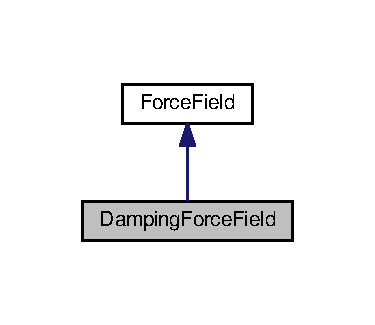
\includegraphics[width=180pt]{classDampingForceField__inherit__graph}
\end{center}
\end{figure}


Collaboration diagram for Damping\+Force\+Field\+:\nopagebreak
\begin{figure}[H]
\begin{center}
\leavevmode
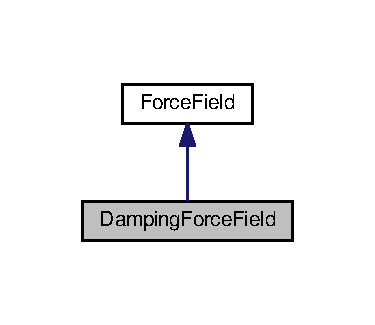
\includegraphics[width=180pt]{classDampingForceField__coll__graph}
\end{center}
\end{figure}
\subsection*{Public Member Functions}
\begin{DoxyCompactItemize}
\item 
\hyperlink{classDampingForceField_ac12609d97690d02099acf10710d2bf3f}{Damping\+Force\+Field} (const std\+::vector$<$ \hyperlink{Particle_8hpp_a9a7abc8635002993537b61ef2c857fdd}{Particle\+Ptr} $>$ particles, const float damping)
\begin{DoxyCompactList}\small\item\em Build a damping force field. \end{DoxyCompactList}\item 
const std\+::vector$<$ \hyperlink{Particle_8hpp_a9a7abc8635002993537b61ef2c857fdd}{Particle\+Ptr} $>$ \hyperlink{classDampingForceField_ace8b8327d3dfd2d6cc58808e301c4542}{get\+Particles} ()
\begin{DoxyCompactList}\small\item\em Access to the particles influenced by this force field. \end{DoxyCompactList}\item 
void \hyperlink{classDampingForceField_a98de1771d2113b73112b602159bf7117}{set\+Particles} (const std\+::vector$<$ \hyperlink{Particle_8hpp_a9a7abc8635002993537b61ef2c857fdd}{Particle\+Ptr} $>$ \&particles)
\begin{DoxyCompactList}\small\item\em Define the set of particles influenced by this force field. \end{DoxyCompactList}\item 
const float \& \hyperlink{classDampingForceField_a02f7ce65355038fa8c29526d4c63d631}{get\+Damping} ()
\begin{DoxyCompactList}\small\item\em Access to the damping factor. \end{DoxyCompactList}\item 
void \hyperlink{classDampingForceField_ae4f282bc01a1b517f76fa7782a70ff6c}{set\+Damping} (const float \&damping)
\begin{DoxyCompactList}\small\item\em Set the damping factor of this force field. \end{DoxyCompactList}\end{DoxyCompactItemize}
\subsection*{Private Member Functions}
\begin{DoxyCompactItemize}
\item 
void \hyperlink{classDampingForceField_a5677c09b83f6f2d13e70e40c08c4e85f}{do\+\_\+add\+Force} ()
\begin{DoxyCompactList}\small\item\em Add force implementation. \end{DoxyCompactList}\end{DoxyCompactItemize}
\subsection*{Private Attributes}
\begin{DoxyCompactItemize}
\item 
std\+::vector$<$ \hyperlink{Particle_8hpp_a9a7abc8635002993537b61ef2c857fdd}{Particle\+Ptr} $>$ \hyperlink{classDampingForceField_acb55824075dc3dfca7c6d2a799d714fa}{m\+\_\+particles}
\item 
float \hyperlink{classDampingForceField_ad84c70d73d5704e9141be637e4d92498}{m\+\_\+damping}
\end{DoxyCompactItemize}


\subsection{Detailed Description}
This class implement a force field that models a damping, i.\+e. a kinetic friction. 

\subsection{Constructor \& Destructor Documentation}
\hypertarget{classDampingForceField_ac12609d97690d02099acf10710d2bf3f}{\index{Damping\+Force\+Field@{Damping\+Force\+Field}!Damping\+Force\+Field@{Damping\+Force\+Field}}
\index{Damping\+Force\+Field@{Damping\+Force\+Field}!Damping\+Force\+Field@{Damping\+Force\+Field}}
\subsubsection[{Damping\+Force\+Field}]{\setlength{\rightskip}{0pt plus 5cm}Damping\+Force\+Field\+::\+Damping\+Force\+Field (
\begin{DoxyParamCaption}
\item[{const std\+::vector$<$ {\bf Particle\+Ptr} $>$}]{particles, }
\item[{const float}]{damping}
\end{DoxyParamCaption}
)}}\label{classDampingForceField_ac12609d97690d02099acf10710d2bf3f}
Build a damping force applied to a set of particles. The force added to a particle of velocity v is -\/damping $\ast$ v. 
\begin{DoxyParams}{Parameters}
{\em particles} & Set of particles influenced by this damping force. \\
\hline
{\em damping} & Damping coefficient. \\
\hline
\end{DoxyParams}


\subsection{Member Function Documentation}
\hypertarget{classDampingForceField_a5677c09b83f6f2d13e70e40c08c4e85f}{\index{Damping\+Force\+Field@{Damping\+Force\+Field}!do\+\_\+add\+Force@{do\+\_\+add\+Force}}
\index{do\+\_\+add\+Force@{do\+\_\+add\+Force}!Damping\+Force\+Field@{Damping\+Force\+Field}}
\subsubsection[{do\+\_\+add\+Force}]{\setlength{\rightskip}{0pt plus 5cm}void Damping\+Force\+Field\+::do\+\_\+add\+Force (
\begin{DoxyParamCaption}
{}
\end{DoxyParamCaption}
)\hspace{0.3cm}{\ttfamily [private]}, {\ttfamily [virtual]}}}\label{classDampingForceField_a5677c09b83f6f2d13e70e40c08c4e85f}
The actual implementation to add force to the particles. This should be implemented in derived classes. 

Implements \hyperlink{classForceField_a2f44520a00188a3aaeb04e667e8d2673}{Force\+Field}.

\hypertarget{classDampingForceField_a02f7ce65355038fa8c29526d4c63d631}{\index{Damping\+Force\+Field@{Damping\+Force\+Field}!get\+Damping@{get\+Damping}}
\index{get\+Damping@{get\+Damping}!Damping\+Force\+Field@{Damping\+Force\+Field}}
\subsubsection[{get\+Damping}]{\setlength{\rightskip}{0pt plus 5cm}const float\& Damping\+Force\+Field\+::get\+Damping (
\begin{DoxyParamCaption}
{}
\end{DoxyParamCaption}
)}}\label{classDampingForceField_a02f7ce65355038fa8c29526d4c63d631}
Get the damping factor of this force field. \begin{DoxyReturn}{Returns}
The damping factor of this. 
\end{DoxyReturn}
\hypertarget{classDampingForceField_ace8b8327d3dfd2d6cc58808e301c4542}{\index{Damping\+Force\+Field@{Damping\+Force\+Field}!get\+Particles@{get\+Particles}}
\index{get\+Particles@{get\+Particles}!Damping\+Force\+Field@{Damping\+Force\+Field}}
\subsubsection[{get\+Particles}]{\setlength{\rightskip}{0pt plus 5cm}const std\+::vector$<${\bf Particle\+Ptr}$>$ Damping\+Force\+Field\+::get\+Particles (
\begin{DoxyParamCaption}
{}
\end{DoxyParamCaption}
)}}\label{classDampingForceField_ace8b8327d3dfd2d6cc58808e301c4542}
Get the particles influenced by this damping force field. \begin{DoxyReturn}{Returns}
The set of particles influenced by this. 
\end{DoxyReturn}
\hypertarget{classDampingForceField_ae4f282bc01a1b517f76fa7782a70ff6c}{\index{Damping\+Force\+Field@{Damping\+Force\+Field}!set\+Damping@{set\+Damping}}
\index{set\+Damping@{set\+Damping}!Damping\+Force\+Field@{Damping\+Force\+Field}}
\subsubsection[{set\+Damping}]{\setlength{\rightskip}{0pt plus 5cm}void Damping\+Force\+Field\+::set\+Damping (
\begin{DoxyParamCaption}
\item[{const float \&}]{damping}
\end{DoxyParamCaption}
)}}\label{classDampingForceField_ae4f282bc01a1b517f76fa7782a70ff6c}
Define the damping factor of this damping force field. 
\begin{DoxyParams}{Parameters}
{\em damping} & The new damping factor. \\
\hline
\end{DoxyParams}
\hypertarget{classDampingForceField_a98de1771d2113b73112b602159bf7117}{\index{Damping\+Force\+Field@{Damping\+Force\+Field}!set\+Particles@{set\+Particles}}
\index{set\+Particles@{set\+Particles}!Damping\+Force\+Field@{Damping\+Force\+Field}}
\subsubsection[{set\+Particles}]{\setlength{\rightskip}{0pt plus 5cm}void Damping\+Force\+Field\+::set\+Particles (
\begin{DoxyParamCaption}
\item[{const std\+::vector$<$ {\bf Particle\+Ptr} $>$ \&}]{particles}
\end{DoxyParamCaption}
)}}\label{classDampingForceField_a98de1771d2113b73112b602159bf7117}
Define the set of particles that will be influenced by this damping force force. 
\begin{DoxyParams}{Parameters}
{\em particles} & The new set of influenced particles. \\
\hline
\end{DoxyParams}


\subsection{Member Data Documentation}
\hypertarget{classDampingForceField_ad84c70d73d5704e9141be637e4d92498}{\index{Damping\+Force\+Field@{Damping\+Force\+Field}!m\+\_\+damping@{m\+\_\+damping}}
\index{m\+\_\+damping@{m\+\_\+damping}!Damping\+Force\+Field@{Damping\+Force\+Field}}
\subsubsection[{m\+\_\+damping}]{\setlength{\rightskip}{0pt plus 5cm}float Damping\+Force\+Field\+::m\+\_\+damping\hspace{0.3cm}{\ttfamily [private]}}}\label{classDampingForceField_ad84c70d73d5704e9141be637e4d92498}
\hypertarget{classDampingForceField_acb55824075dc3dfca7c6d2a799d714fa}{\index{Damping\+Force\+Field@{Damping\+Force\+Field}!m\+\_\+particles@{m\+\_\+particles}}
\index{m\+\_\+particles@{m\+\_\+particles}!Damping\+Force\+Field@{Damping\+Force\+Field}}
\subsubsection[{m\+\_\+particles}]{\setlength{\rightskip}{0pt plus 5cm}std\+::vector$<${\bf Particle\+Ptr}$>$ Damping\+Force\+Field\+::m\+\_\+particles\hspace{0.3cm}{\ttfamily [private]}}}\label{classDampingForceField_acb55824075dc3dfca7c6d2a799d714fa}


The documentation for this class was generated from the following file\+:\begin{DoxyCompactItemize}
\item 
/home/chardon/\+Depot/ensimag/2\+A\+\_\+\+G3\+D/practicals/teacher\+Source/include/dynamics/\hyperlink{DampingForceField_8hpp}{Damping\+Force\+Field.\+hpp}\end{DoxyCompactItemize}

\hypertarget{classDirectionalLight}{\section{Directional\+Light Class Reference}
\label{classDirectionalLight}\index{Directional\+Light@{Directional\+Light}}
}


A directional light.  




{\ttfamily \#include $<$Light.\+hpp$>$}

\subsection*{Public Types}
\begin{DoxyCompactItemize}
\item 
typedef std\+::shared\+\_\+ptr\\*
$<$ \hyperlink{classDirectionalLight}{Directional\+Light} $>$ \hyperlink{classDirectionalLight_abb43c478c01d5e7c158699e9f3661bce}{Directional\+Light\+Ptr}
\end{DoxyCompactItemize}
\subsection*{Public Member Functions}
\begin{DoxyCompactItemize}
\item 
\hyperlink{classDirectionalLight_ac4aca6c806e752c65ffea9b2f237b245}{$\sim$\+Directional\+Light} ()
\begin{DoxyCompactList}\small\item\em Destructor. \end{DoxyCompactList}\item 
\hyperlink{classDirectionalLight_a949b877ae041b9818f47eb812d80fa1b}{Directional\+Light} ()
\begin{DoxyCompactList}\small\item\em Default constructor. \end{DoxyCompactList}\item 
\hyperlink{classDirectionalLight_aa2f0352247094325d9496a7883fc7ba4}{Directional\+Light} (const \hyperlink{classDirectionalLight}{Directional\+Light} \&directional\+Light)
\begin{DoxyCompactList}\small\item\em Copy constructor. \end{DoxyCompactList}\item 
\hyperlink{classDirectionalLight_a27bae6211ab086bd175291e8de5c6c2b}{Directional\+Light} (const glm\+::vec3 \&\hyperlink{classDirectionalLight_a62bcb380d9e81abc20185b990ef35ec8}{direction}, const glm\+::vec3 \&\hyperlink{classDirectionalLight_a348fa5150e5959b26411715b6ba1bff2}{ambient}, const glm\+::vec3 \&\hyperlink{classDirectionalLight_ab0314fdc6fb9722f4bf17c198df348f9}{diffuse}, const glm\+::vec3 \&\hyperlink{classDirectionalLight_a46773cdc52f5a93e05c25a1742257312}{specular})
\begin{DoxyCompactList}\small\item\em Specific constructor. \end{DoxyCompactList}\item 
const glm\+::vec3 \& \hyperlink{classDirectionalLight_a62bcb380d9e81abc20185b990ef35ec8}{direction} () const 
\begin{DoxyCompactList}\small\item\em Access to the direction of the light. \end{DoxyCompactList}\item 
void \hyperlink{classDirectionalLight_a48a2fca768a442accf005ffa8e2917d8}{set\+Direction} (const glm\+::vec3 \&\hyperlink{classDirectionalLight_a62bcb380d9e81abc20185b990ef35ec8}{direction})
\begin{DoxyCompactList}\small\item\em Set the direction of the light. \end{DoxyCompactList}\item 
const glm\+::vec3 \& \hyperlink{classDirectionalLight_a348fa5150e5959b26411715b6ba1bff2}{ambient} () const 
\begin{DoxyCompactList}\small\item\em Access to the ambient intensity of the light. \end{DoxyCompactList}\item 
void \hyperlink{classDirectionalLight_ad2317a4398d25c19c0c7ecda894a9e03}{set\+Ambient} (const glm\+::vec3 \&\hyperlink{classDirectionalLight_a348fa5150e5959b26411715b6ba1bff2}{ambient})
\begin{DoxyCompactList}\small\item\em Set the ambient intensity of the light. \end{DoxyCompactList}\item 
const glm\+::vec3 \& \hyperlink{classDirectionalLight_ab0314fdc6fb9722f4bf17c198df348f9}{diffuse} () const 
\begin{DoxyCompactList}\small\item\em Access to the diffuse intensity of the light. \end{DoxyCompactList}\item 
void \hyperlink{classDirectionalLight_ab646ca1453dd80a76fa333ae74576bf4}{set\+Diffuse} (const glm\+::vec3 \&\hyperlink{classDirectionalLight_ab0314fdc6fb9722f4bf17c198df348f9}{diffuse})
\begin{DoxyCompactList}\small\item\em Set the diffuse intensity of the light. \end{DoxyCompactList}\item 
const glm\+::vec3 \& \hyperlink{classDirectionalLight_a46773cdc52f5a93e05c25a1742257312}{specular} () const 
\begin{DoxyCompactList}\small\item\em Access to the specular intensity of the light. \end{DoxyCompactList}\item 
void \hyperlink{classDirectionalLight_aaf7612501976569deb935ee0dc70eda5}{set\+Specular} (const glm\+::vec3 \&\hyperlink{classDirectionalLight_a46773cdc52f5a93e05c25a1742257312}{specular})
\begin{DoxyCompactList}\small\item\em Set the specular intensity of the light. \end{DoxyCompactList}\end{DoxyCompactItemize}
\subsection*{Static Public Member Functions}
\begin{DoxyCompactItemize}
\item 
static bool \hyperlink{classDirectionalLight_a0dbd9593486ae29871f6cce9f62a9b2b}{send\+To\+G\+P\+U} (const \hyperlink{ShaderProgram_8hpp_af8e4af1ad4c53875ee5d32ab7e1f4966}{Shader\+Program\+Ptr} \&program, const \hyperlink{classDirectionalLight_abb43c478c01d5e7c158699e9f3661bce}{Directional\+Light\+Ptr} \&light)
\begin{DoxyCompactList}\small\item\em Get location for the attributes of the light and send the data to the G\+P\+U as uniforms. \end{DoxyCompactList}\end{DoxyCompactItemize}
\subsection*{Private Member Functions}
\begin{DoxyCompactItemize}
\item 
std\+::string \hyperlink{classDirectionalLight_ac3320ddae5142ae1e96db3b4e6874ff4}{light\+Name} ()
\begin{DoxyCompactList}\small\item\em Get the uniform name of the light. \end{DoxyCompactList}\item 
std\+::string \hyperlink{classDirectionalLight_a7f77772f2c797d04935d7c041bb7c717}{direction\+Name} ()
\begin{DoxyCompactList}\small\item\em Get the uniform name of the direction of the light. \end{DoxyCompactList}\item 
std\+::string \hyperlink{classDirectionalLight_a028a58bf7d60840548f85339086d2607}{ambient\+Name} ()
\begin{DoxyCompactList}\small\item\em Get the uniform name of the ambient intensity of the light. \end{DoxyCompactList}\item 
std\+::string \hyperlink{classDirectionalLight_a8226d712ae3399d6e90ce2ffa55b7f2d}{diffuse\+Name} ()
\begin{DoxyCompactList}\small\item\em Get the uniform name of the diffuse intensity of the light. \end{DoxyCompactList}\item 
std\+::string \hyperlink{classDirectionalLight_ac08e88f445126ad6f26be6459aead7ba}{specular\+Name} ()
\begin{DoxyCompactList}\small\item\em Get the uniform name of the specular intensity of the light. \end{DoxyCompactList}\end{DoxyCompactItemize}
\subsection*{Private Attributes}
\begin{DoxyCompactItemize}
\item 
glm\+::vec3 \hyperlink{classDirectionalLight_a4432e8ebaa81b9fe4d033056eb19ca4c}{m\+\_\+direction}
\item 
glm\+::vec3 \hyperlink{classDirectionalLight_afaf3088136b72d8af8188526e410b53a}{m\+\_\+ambient}
\item 
glm\+::vec3 \hyperlink{classDirectionalLight_aa9391a104441f2cb5cc56e976bcde89a}{m\+\_\+diffuse}
\item 
glm\+::vec3 \hyperlink{classDirectionalLight_a56e4161550e3eaa31d17c54cf108a028}{m\+\_\+specular}
\end{DoxyCompactItemize}


\subsection{Detailed Description}
This class represents a directional light which means a light whose source is so far away from the camera that the light rays can be considered close to parallel from each other regardless of the position of the objects or the camera. A good example is the sun. 

\subsection{Member Typedef Documentation}
\hypertarget{classDirectionalLight_abb43c478c01d5e7c158699e9f3661bce}{\index{Directional\+Light@{Directional\+Light}!Directional\+Light\+Ptr@{Directional\+Light\+Ptr}}
\index{Directional\+Light\+Ptr@{Directional\+Light\+Ptr}!Directional\+Light@{Directional\+Light}}
\subsubsection[{Directional\+Light\+Ptr}]{\setlength{\rightskip}{0pt plus 5cm}typedef std\+::shared\+\_\+ptr$<${\bf Directional\+Light}$>$ {\bf Directional\+Light\+::\+Directional\+Light\+Ptr}}}\label{classDirectionalLight_abb43c478c01d5e7c158699e9f3661bce}
Smart pointer to a directional light 

\subsection{Constructor \& Destructor Documentation}
\hypertarget{classDirectionalLight_ac4aca6c806e752c65ffea9b2f237b245}{\index{Directional\+Light@{Directional\+Light}!````~Directional\+Light@{$\sim$\+Directional\+Light}}
\index{````~Directional\+Light@{$\sim$\+Directional\+Light}!Directional\+Light@{Directional\+Light}}
\subsubsection[{$\sim$\+Directional\+Light}]{\setlength{\rightskip}{0pt plus 5cm}Directional\+Light\+::$\sim$\+Directional\+Light (
\begin{DoxyParamCaption}
{}
\end{DoxyParamCaption}
)}}\label{classDirectionalLight_ac4aca6c806e752c65ffea9b2f237b245}
\hypertarget{classDirectionalLight_a949b877ae041b9818f47eb812d80fa1b}{\index{Directional\+Light@{Directional\+Light}!Directional\+Light@{Directional\+Light}}
\index{Directional\+Light@{Directional\+Light}!Directional\+Light@{Directional\+Light}}
\subsubsection[{Directional\+Light}]{\setlength{\rightskip}{0pt plus 5cm}Directional\+Light\+::\+Directional\+Light (
\begin{DoxyParamCaption}
{}
\end{DoxyParamCaption}
)}}\label{classDirectionalLight_a949b877ae041b9818f47eb812d80fa1b}
\hypertarget{classDirectionalLight_aa2f0352247094325d9496a7883fc7ba4}{\index{Directional\+Light@{Directional\+Light}!Directional\+Light@{Directional\+Light}}
\index{Directional\+Light@{Directional\+Light}!Directional\+Light@{Directional\+Light}}
\subsubsection[{Directional\+Light}]{\setlength{\rightskip}{0pt plus 5cm}Directional\+Light\+::\+Directional\+Light (
\begin{DoxyParamCaption}
\item[{const {\bf Directional\+Light} \&}]{directional\+Light}
\end{DoxyParamCaption}
)}}\label{classDirectionalLight_aa2f0352247094325d9496a7883fc7ba4}
\hypertarget{classDirectionalLight_a27bae6211ab086bd175291e8de5c6c2b}{\index{Directional\+Light@{Directional\+Light}!Directional\+Light@{Directional\+Light}}
\index{Directional\+Light@{Directional\+Light}!Directional\+Light@{Directional\+Light}}
\subsubsection[{Directional\+Light}]{\setlength{\rightskip}{0pt plus 5cm}Directional\+Light\+::\+Directional\+Light (
\begin{DoxyParamCaption}
\item[{const glm\+::vec3 \&}]{direction, }
\item[{const glm\+::vec3 \&}]{ambient, }
\item[{const glm\+::vec3 \&}]{diffuse, }
\item[{const glm\+::vec3 \&}]{specular}
\end{DoxyParamCaption}
)}}\label{classDirectionalLight_a27bae6211ab086bd175291e8de5c6c2b}
Construct a directional light.


\begin{DoxyParams}{Parameters}
{\em direction} & The direction of the light. \\
\hline
{\em ambient} & The ambient intensity of the light. \\
\hline
{\em diffuse} & The diffuse intensity of the light. \\
\hline
{\em specular} & The specular intensity of the light. \\
\hline
\end{DoxyParams}


\subsection{Member Function Documentation}
\hypertarget{classDirectionalLight_a348fa5150e5959b26411715b6ba1bff2}{\index{Directional\+Light@{Directional\+Light}!ambient@{ambient}}
\index{ambient@{ambient}!Directional\+Light@{Directional\+Light}}
\subsubsection[{ambient}]{\setlength{\rightskip}{0pt plus 5cm}const glm\+::vec3\& Directional\+Light\+::ambient (
\begin{DoxyParamCaption}
{}
\end{DoxyParamCaption}
) const}}\label{classDirectionalLight_a348fa5150e5959b26411715b6ba1bff2}
\begin{DoxyReturn}{Returns}
A const reference to m\+\_\+ambient. 
\end{DoxyReturn}
\hypertarget{classDirectionalLight_a028a58bf7d60840548f85339086d2607}{\index{Directional\+Light@{Directional\+Light}!ambient\+Name@{ambient\+Name}}
\index{ambient\+Name@{ambient\+Name}!Directional\+Light@{Directional\+Light}}
\subsubsection[{ambient\+Name}]{\setlength{\rightskip}{0pt plus 5cm}std\+::string Directional\+Light\+::ambient\+Name (
\begin{DoxyParamCaption}
{}
\end{DoxyParamCaption}
)\hspace{0.3cm}{\ttfamily [inline]}, {\ttfamily [private]}}}\label{classDirectionalLight_a028a58bf7d60840548f85339086d2607}
\begin{DoxyReturn}{Returns}
The name of the ambient intensity of the light in the shader. 
\end{DoxyReturn}
\hypertarget{classDirectionalLight_ab0314fdc6fb9722f4bf17c198df348f9}{\index{Directional\+Light@{Directional\+Light}!diffuse@{diffuse}}
\index{diffuse@{diffuse}!Directional\+Light@{Directional\+Light}}
\subsubsection[{diffuse}]{\setlength{\rightskip}{0pt plus 5cm}const glm\+::vec3\& Directional\+Light\+::diffuse (
\begin{DoxyParamCaption}
{}
\end{DoxyParamCaption}
) const}}\label{classDirectionalLight_ab0314fdc6fb9722f4bf17c198df348f9}
\begin{DoxyReturn}{Returns}
A const reference to m\+\_\+diffuse. 
\end{DoxyReturn}
\hypertarget{classDirectionalLight_a8226d712ae3399d6e90ce2ffa55b7f2d}{\index{Directional\+Light@{Directional\+Light}!diffuse\+Name@{diffuse\+Name}}
\index{diffuse\+Name@{diffuse\+Name}!Directional\+Light@{Directional\+Light}}
\subsubsection[{diffuse\+Name}]{\setlength{\rightskip}{0pt plus 5cm}std\+::string Directional\+Light\+::diffuse\+Name (
\begin{DoxyParamCaption}
{}
\end{DoxyParamCaption}
)\hspace{0.3cm}{\ttfamily [inline]}, {\ttfamily [private]}}}\label{classDirectionalLight_a8226d712ae3399d6e90ce2ffa55b7f2d}
\begin{DoxyReturn}{Returns}
The name of the diffuse intensity of the light in the shader. 
\end{DoxyReturn}
\hypertarget{classDirectionalLight_a62bcb380d9e81abc20185b990ef35ec8}{\index{Directional\+Light@{Directional\+Light}!direction@{direction}}
\index{direction@{direction}!Directional\+Light@{Directional\+Light}}
\subsubsection[{direction}]{\setlength{\rightskip}{0pt plus 5cm}const glm\+::vec3\& Directional\+Light\+::direction (
\begin{DoxyParamCaption}
{}
\end{DoxyParamCaption}
) const}}\label{classDirectionalLight_a62bcb380d9e81abc20185b990ef35ec8}
\begin{DoxyReturn}{Returns}
A const reference to m\+\_\+direction. 
\end{DoxyReturn}
\hypertarget{classDirectionalLight_a7f77772f2c797d04935d7c041bb7c717}{\index{Directional\+Light@{Directional\+Light}!direction\+Name@{direction\+Name}}
\index{direction\+Name@{direction\+Name}!Directional\+Light@{Directional\+Light}}
\subsubsection[{direction\+Name}]{\setlength{\rightskip}{0pt plus 5cm}std\+::string Directional\+Light\+::direction\+Name (
\begin{DoxyParamCaption}
{}
\end{DoxyParamCaption}
)\hspace{0.3cm}{\ttfamily [inline]}, {\ttfamily [private]}}}\label{classDirectionalLight_a7f77772f2c797d04935d7c041bb7c717}
\begin{DoxyReturn}{Returns}
The name of the direction of the light in the shader. 
\end{DoxyReturn}
\hypertarget{classDirectionalLight_ac3320ddae5142ae1e96db3b4e6874ff4}{\index{Directional\+Light@{Directional\+Light}!light\+Name@{light\+Name}}
\index{light\+Name@{light\+Name}!Directional\+Light@{Directional\+Light}}
\subsubsection[{light\+Name}]{\setlength{\rightskip}{0pt plus 5cm}std\+::string Directional\+Light\+::light\+Name (
\begin{DoxyParamCaption}
{}
\end{DoxyParamCaption}
)\hspace{0.3cm}{\ttfamily [inline]}, {\ttfamily [private]}}}\label{classDirectionalLight_ac3320ddae5142ae1e96db3b4e6874ff4}
\begin{DoxyReturn}{Returns}
The name of the light in the shader. 
\end{DoxyReturn}
\hypertarget{classDirectionalLight_a0dbd9593486ae29871f6cce9f62a9b2b}{\index{Directional\+Light@{Directional\+Light}!send\+To\+G\+P\+U@{send\+To\+G\+P\+U}}
\index{send\+To\+G\+P\+U@{send\+To\+G\+P\+U}!Directional\+Light@{Directional\+Light}}
\subsubsection[{send\+To\+G\+P\+U}]{\setlength{\rightskip}{0pt plus 5cm}static bool Directional\+Light\+::send\+To\+G\+P\+U (
\begin{DoxyParamCaption}
\item[{const {\bf Shader\+Program\+Ptr} \&}]{program, }
\item[{const {\bf Directional\+Light\+Ptr} \&}]{light}
\end{DoxyParamCaption}
)\hspace{0.3cm}{\ttfamily [static]}}}\label{classDirectionalLight_a0dbd9593486ae29871f6cce9f62a9b2b}

\begin{DoxyParams}{Parameters}
{\em program} & A pointer to the shader program where to get the locations. \\
\hline
{\em light} & A pointer to the light to send to the G\+P\+U. \\
\hline
\end{DoxyParams}
\begin{DoxyReturn}{Returns}
True if everything was fine, false otherwise 
\end{DoxyReturn}
\hypertarget{classDirectionalLight_ad2317a4398d25c19c0c7ecda894a9e03}{\index{Directional\+Light@{Directional\+Light}!set\+Ambient@{set\+Ambient}}
\index{set\+Ambient@{set\+Ambient}!Directional\+Light@{Directional\+Light}}
\subsubsection[{set\+Ambient}]{\setlength{\rightskip}{0pt plus 5cm}void Directional\+Light\+::set\+Ambient (
\begin{DoxyParamCaption}
\item[{const glm\+::vec3 \&}]{ambient}
\end{DoxyParamCaption}
)}}\label{classDirectionalLight_ad2317a4398d25c19c0c7ecda894a9e03}
Set the value of m\+\_\+ambient. 
\begin{DoxyParams}{Parameters}
{\em ambient} & The new ambient intensity of the light. \\
\hline
\end{DoxyParams}
\hypertarget{classDirectionalLight_ab646ca1453dd80a76fa333ae74576bf4}{\index{Directional\+Light@{Directional\+Light}!set\+Diffuse@{set\+Diffuse}}
\index{set\+Diffuse@{set\+Diffuse}!Directional\+Light@{Directional\+Light}}
\subsubsection[{set\+Diffuse}]{\setlength{\rightskip}{0pt plus 5cm}void Directional\+Light\+::set\+Diffuse (
\begin{DoxyParamCaption}
\item[{const glm\+::vec3 \&}]{diffuse}
\end{DoxyParamCaption}
)}}\label{classDirectionalLight_ab646ca1453dd80a76fa333ae74576bf4}
Set the value of m\+\_\+diffuse. 
\begin{DoxyParams}{Parameters}
{\em diffuse} & The new diffuse intensity of the light. \\
\hline
\end{DoxyParams}
\hypertarget{classDirectionalLight_a48a2fca768a442accf005ffa8e2917d8}{\index{Directional\+Light@{Directional\+Light}!set\+Direction@{set\+Direction}}
\index{set\+Direction@{set\+Direction}!Directional\+Light@{Directional\+Light}}
\subsubsection[{set\+Direction}]{\setlength{\rightskip}{0pt plus 5cm}void Directional\+Light\+::set\+Direction (
\begin{DoxyParamCaption}
\item[{const glm\+::vec3 \&}]{direction}
\end{DoxyParamCaption}
)}}\label{classDirectionalLight_a48a2fca768a442accf005ffa8e2917d8}
Set the value of m\+\_\+direction. 
\begin{DoxyParams}{Parameters}
{\em direction} & The new direction of the light. \\
\hline
\end{DoxyParams}
\hypertarget{classDirectionalLight_aaf7612501976569deb935ee0dc70eda5}{\index{Directional\+Light@{Directional\+Light}!set\+Specular@{set\+Specular}}
\index{set\+Specular@{set\+Specular}!Directional\+Light@{Directional\+Light}}
\subsubsection[{set\+Specular}]{\setlength{\rightskip}{0pt plus 5cm}void Directional\+Light\+::set\+Specular (
\begin{DoxyParamCaption}
\item[{const glm\+::vec3 \&}]{specular}
\end{DoxyParamCaption}
)}}\label{classDirectionalLight_aaf7612501976569deb935ee0dc70eda5}
Set the value of m\+\_\+specular. 
\begin{DoxyParams}{Parameters}
{\em specular} & The new specular intensity of the light. \\
\hline
\end{DoxyParams}
\hypertarget{classDirectionalLight_a46773cdc52f5a93e05c25a1742257312}{\index{Directional\+Light@{Directional\+Light}!specular@{specular}}
\index{specular@{specular}!Directional\+Light@{Directional\+Light}}
\subsubsection[{specular}]{\setlength{\rightskip}{0pt plus 5cm}const glm\+::vec3\& Directional\+Light\+::specular (
\begin{DoxyParamCaption}
{}
\end{DoxyParamCaption}
) const}}\label{classDirectionalLight_a46773cdc52f5a93e05c25a1742257312}
\begin{DoxyReturn}{Returns}
A const reference to m\+\_\+specular. 
\end{DoxyReturn}
\hypertarget{classDirectionalLight_ac08e88f445126ad6f26be6459aead7ba}{\index{Directional\+Light@{Directional\+Light}!specular\+Name@{specular\+Name}}
\index{specular\+Name@{specular\+Name}!Directional\+Light@{Directional\+Light}}
\subsubsection[{specular\+Name}]{\setlength{\rightskip}{0pt plus 5cm}std\+::string Directional\+Light\+::specular\+Name (
\begin{DoxyParamCaption}
{}
\end{DoxyParamCaption}
)\hspace{0.3cm}{\ttfamily [inline]}, {\ttfamily [private]}}}\label{classDirectionalLight_ac08e88f445126ad6f26be6459aead7ba}
\begin{DoxyReturn}{Returns}
The name of the specular intensity of the light in the shader. 
\end{DoxyReturn}


\subsection{Member Data Documentation}
\hypertarget{classDirectionalLight_afaf3088136b72d8af8188526e410b53a}{\index{Directional\+Light@{Directional\+Light}!m\+\_\+ambient@{m\+\_\+ambient}}
\index{m\+\_\+ambient@{m\+\_\+ambient}!Directional\+Light@{Directional\+Light}}
\subsubsection[{m\+\_\+ambient}]{\setlength{\rightskip}{0pt plus 5cm}glm\+::vec3 Directional\+Light\+::m\+\_\+ambient\hspace{0.3cm}{\ttfamily [private]}}}\label{classDirectionalLight_afaf3088136b72d8af8188526e410b53a}
Intensity of the light with respect to the object ambient components. \hypertarget{classDirectionalLight_aa9391a104441f2cb5cc56e976bcde89a}{\index{Directional\+Light@{Directional\+Light}!m\+\_\+diffuse@{m\+\_\+diffuse}}
\index{m\+\_\+diffuse@{m\+\_\+diffuse}!Directional\+Light@{Directional\+Light}}
\subsubsection[{m\+\_\+diffuse}]{\setlength{\rightskip}{0pt plus 5cm}glm\+::vec3 Directional\+Light\+::m\+\_\+diffuse\hspace{0.3cm}{\ttfamily [private]}}}\label{classDirectionalLight_aa9391a104441f2cb5cc56e976bcde89a}
Intensity of the light with respect to the object diffuse components. \hypertarget{classDirectionalLight_a4432e8ebaa81b9fe4d033056eb19ca4c}{\index{Directional\+Light@{Directional\+Light}!m\+\_\+direction@{m\+\_\+direction}}
\index{m\+\_\+direction@{m\+\_\+direction}!Directional\+Light@{Directional\+Light}}
\subsubsection[{m\+\_\+direction}]{\setlength{\rightskip}{0pt plus 5cm}glm\+::vec3 Directional\+Light\+::m\+\_\+direction\hspace{0.3cm}{\ttfamily [private]}}}\label{classDirectionalLight_a4432e8ebaa81b9fe4d033056eb19ca4c}
The direction of the light. \hypertarget{classDirectionalLight_a56e4161550e3eaa31d17c54cf108a028}{\index{Directional\+Light@{Directional\+Light}!m\+\_\+specular@{m\+\_\+specular}}
\index{m\+\_\+specular@{m\+\_\+specular}!Directional\+Light@{Directional\+Light}}
\subsubsection[{m\+\_\+specular}]{\setlength{\rightskip}{0pt plus 5cm}glm\+::vec3 Directional\+Light\+::m\+\_\+specular\hspace{0.3cm}{\ttfamily [private]}}}\label{classDirectionalLight_a56e4161550e3eaa31d17c54cf108a028}
Intensity of the light with respect to the object specular components. 

The documentation for this class was generated from the following file\+:\begin{DoxyCompactItemize}
\item 
/home/chardon/\+Depot/ensimag/2\+A\+\_\+\+G3\+D/practicals/teacher\+Source/include/lighting/\hyperlink{Light_8hpp}{Light.\+hpp}\end{DoxyCompactItemize}

\hypertarget{classDirectionalLightRenderable}{\section{Directional\+Light\+Renderable Class Reference}
\label{classDirectionalLightRenderable}\index{Directional\+Light\+Renderable@{Directional\+Light\+Renderable}}
}


{\ttfamily \#include $<$Directional\+Light\+Renderable.\+hpp$>$}



Inheritance diagram for Directional\+Light\+Renderable\+:\nopagebreak
\begin{figure}[H]
\begin{center}
\leavevmode
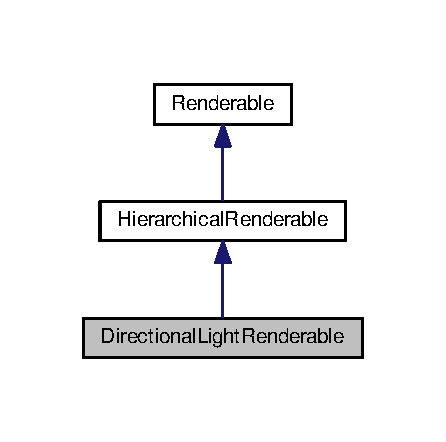
\includegraphics[width=214pt]{classDirectionalLightRenderable__inherit__graph}
\end{center}
\end{figure}


Collaboration diagram for Directional\+Light\+Renderable\+:\nopagebreak
\begin{figure}[H]
\begin{center}
\leavevmode
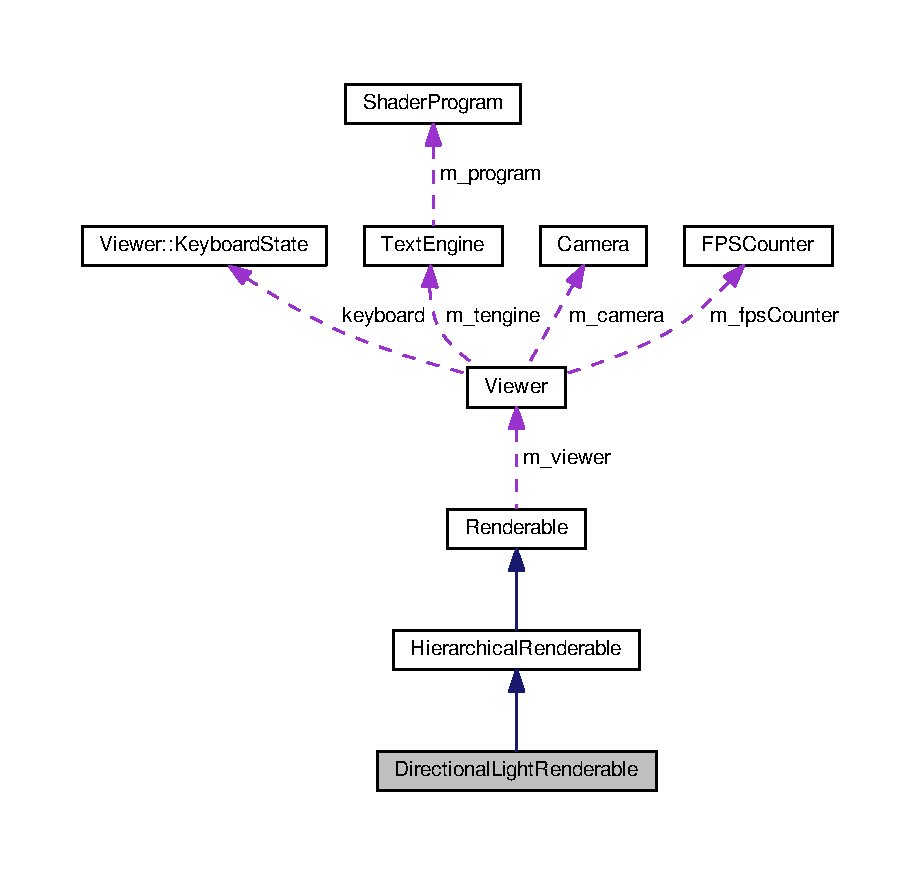
\includegraphics[width=350pt]{classDirectionalLightRenderable__coll__graph}
\end{center}
\end{figure}
\subsection*{Public Member Functions}
\begin{DoxyCompactItemize}
\item 
\hyperlink{classDirectionalLightRenderable_aa91073f6a38fbb29c14fdc3b22474fd4}{$\sim$\+Directional\+Light\+Renderable} ()
\item 
\hyperlink{classDirectionalLightRenderable_ab3f213298b946e718834c51e56ad3713}{Directional\+Light\+Renderable} (\hyperlink{ShaderProgram_8hpp_af8e4af1ad4c53875ee5d32ab7e1f4966}{Shader\+Program\+Ptr} program, \hyperlink{Light_8hpp_ad8ef93288a101a8d8f185fb2a88f496d}{Directional\+Light\+Ptr} light, const glm\+::vec3 \&\hyperlink{classDirectionalLightRenderable_a7954a6f447fcf82f9669a4abc1f45b59}{position})
\item 
glm\+::vec3 \hyperlink{classDirectionalLightRenderable_a7954a6f447fcf82f9669a4abc1f45b59}{position} () const 
\item 
void \hyperlink{classDirectionalLightRenderable_aae92546ac8ae14e814594fdb20ceb543}{set\+Position} (const glm\+::vec3 \&\hyperlink{classDirectionalLightRenderable_a7954a6f447fcf82f9669a4abc1f45b59}{position})
\end{DoxyCompactItemize}
\subsection*{Private Member Functions}
\begin{DoxyCompactItemize}
\item 
void \hyperlink{classDirectionalLightRenderable_a9560a1e6c2b525de69140ab0d8059734}{do\+\_\+draw} ()
\begin{DoxyCompactList}\small\item\em Draw virtual function. \end{DoxyCompactList}\item 
void \hyperlink{classDirectionalLightRenderable_a7caf2f55742229944de3f6a9ee3f27ac}{do\+\_\+animate} (float time)
\begin{DoxyCompactList}\small\item\em Animate virtual function. \end{DoxyCompactList}\end{DoxyCompactItemize}
\subsection*{Private Attributes}
\begin{DoxyCompactItemize}
\item 
glm\+::vec3 \hyperlink{classDirectionalLightRenderable_aa5d35d4b87584a1a1fd44c0aaa6583cd}{m\+\_\+position}
\item 
std\+::vector$<$ glm\+::vec3 $>$ \hyperlink{classDirectionalLightRenderable_a75710cee9753842958f58c4ef34bf0e9}{m\+\_\+positions}
\item 
std\+::vector$<$ glm\+::vec4 $>$ \hyperlink{classDirectionalLightRenderable_a74752273696bdaf32922d0588eb5ffbe}{m\+\_\+colors}
\item 
std\+::vector$<$ glm\+::vec3 $>$ \hyperlink{classDirectionalLightRenderable_a2300d0c32113e49e1078e52ea59cfd2c}{m\+\_\+normals}
\item 
unsigned int \hyperlink{classDirectionalLightRenderable_aaa4a4aa8e51d7d1acec1586b207fd00c}{m\+\_\+p\+Buffer}
\item 
unsigned int \hyperlink{classDirectionalLightRenderable_a0127ba14dca5423b39dd3fc48f9f320b}{m\+\_\+c\+Buffer}
\item 
unsigned int \hyperlink{classDirectionalLightRenderable_afb94e4253a5c4af4a6cd25b443b71ba4}{m\+\_\+n\+Buffer}
\item 
\hyperlink{Light_8hpp_ad8ef93288a101a8d8f185fb2a88f496d}{Directional\+Light\+Ptr} \hyperlink{classDirectionalLightRenderable_a9486047a7b997642ce897b0d4e241d19}{m\+\_\+light}
\end{DoxyCompactItemize}
\subsection*{Additional Inherited Members}


\subsection{Constructor \& Destructor Documentation}
\hypertarget{classDirectionalLightRenderable_aa91073f6a38fbb29c14fdc3b22474fd4}{\index{Directional\+Light\+Renderable@{Directional\+Light\+Renderable}!````~Directional\+Light\+Renderable@{$\sim$\+Directional\+Light\+Renderable}}
\index{````~Directional\+Light\+Renderable@{$\sim$\+Directional\+Light\+Renderable}!Directional\+Light\+Renderable@{Directional\+Light\+Renderable}}
\subsubsection[{$\sim$\+Directional\+Light\+Renderable}]{\setlength{\rightskip}{0pt plus 5cm}Directional\+Light\+Renderable\+::$\sim$\+Directional\+Light\+Renderable (
\begin{DoxyParamCaption}
{}
\end{DoxyParamCaption}
)}}\label{classDirectionalLightRenderable_aa91073f6a38fbb29c14fdc3b22474fd4}
\hypertarget{classDirectionalLightRenderable_ab3f213298b946e718834c51e56ad3713}{\index{Directional\+Light\+Renderable@{Directional\+Light\+Renderable}!Directional\+Light\+Renderable@{Directional\+Light\+Renderable}}
\index{Directional\+Light\+Renderable@{Directional\+Light\+Renderable}!Directional\+Light\+Renderable@{Directional\+Light\+Renderable}}
\subsubsection[{Directional\+Light\+Renderable}]{\setlength{\rightskip}{0pt plus 5cm}Directional\+Light\+Renderable\+::\+Directional\+Light\+Renderable (
\begin{DoxyParamCaption}
\item[{{\bf Shader\+Program\+Ptr}}]{program, }
\item[{{\bf Directional\+Light\+Ptr}}]{light, }
\item[{const glm\+::vec3 \&}]{position}
\end{DoxyParamCaption}
)}}\label{classDirectionalLightRenderable_ab3f213298b946e718834c51e56ad3713}


\subsection{Member Function Documentation}
\hypertarget{classDirectionalLightRenderable_a7caf2f55742229944de3f6a9ee3f27ac}{\index{Directional\+Light\+Renderable@{Directional\+Light\+Renderable}!do\+\_\+animate@{do\+\_\+animate}}
\index{do\+\_\+animate@{do\+\_\+animate}!Directional\+Light\+Renderable@{Directional\+Light\+Renderable}}
\subsubsection[{do\+\_\+animate}]{\setlength{\rightskip}{0pt plus 5cm}void Directional\+Light\+Renderable\+::do\+\_\+animate (
\begin{DoxyParamCaption}
\item[{float}]{time}
\end{DoxyParamCaption}
)\hspace{0.3cm}{\ttfamily [private]}, {\ttfamily [virtual]}}}\label{classDirectionalLightRenderable_a7caf2f55742229944de3f6a9ee3f27ac}
Implementation to animate this renderable. 
\begin{DoxyParams}{Parameters}
{\em time} & The current simulation time. \\
\hline
\end{DoxyParams}


Implements \hyperlink{classRenderable_aa5206322555c9dece40b21e797629b34}{Renderable}.

\hypertarget{classDirectionalLightRenderable_a9560a1e6c2b525de69140ab0d8059734}{\index{Directional\+Light\+Renderable@{Directional\+Light\+Renderable}!do\+\_\+draw@{do\+\_\+draw}}
\index{do\+\_\+draw@{do\+\_\+draw}!Directional\+Light\+Renderable@{Directional\+Light\+Renderable}}
\subsubsection[{do\+\_\+draw}]{\setlength{\rightskip}{0pt plus 5cm}void Directional\+Light\+Renderable\+::do\+\_\+draw (
\begin{DoxyParamCaption}
{}
\end{DoxyParamCaption}
)\hspace{0.3cm}{\ttfamily [private]}, {\ttfamily [virtual]}}}\label{classDirectionalLightRenderable_a9560a1e6c2b525de69140ab0d8059734}
Implementation to draw this renderable. 

Implements \hyperlink{classRenderable_a98ab6308c1d2b56dacda7c435fb38d5b}{Renderable}.

\hypertarget{classDirectionalLightRenderable_a7954a6f447fcf82f9669a4abc1f45b59}{\index{Directional\+Light\+Renderable@{Directional\+Light\+Renderable}!position@{position}}
\index{position@{position}!Directional\+Light\+Renderable@{Directional\+Light\+Renderable}}
\subsubsection[{position}]{\setlength{\rightskip}{0pt plus 5cm}glm\+::vec3 Directional\+Light\+Renderable\+::position (
\begin{DoxyParamCaption}
{}
\end{DoxyParamCaption}
) const}}\label{classDirectionalLightRenderable_a7954a6f447fcf82f9669a4abc1f45b59}
\hypertarget{classDirectionalLightRenderable_aae92546ac8ae14e814594fdb20ceb543}{\index{Directional\+Light\+Renderable@{Directional\+Light\+Renderable}!set\+Position@{set\+Position}}
\index{set\+Position@{set\+Position}!Directional\+Light\+Renderable@{Directional\+Light\+Renderable}}
\subsubsection[{set\+Position}]{\setlength{\rightskip}{0pt plus 5cm}void Directional\+Light\+Renderable\+::set\+Position (
\begin{DoxyParamCaption}
\item[{const glm\+::vec3 \&}]{position}
\end{DoxyParamCaption}
)}}\label{classDirectionalLightRenderable_aae92546ac8ae14e814594fdb20ceb543}


\subsection{Member Data Documentation}
\hypertarget{classDirectionalLightRenderable_a0127ba14dca5423b39dd3fc48f9f320b}{\index{Directional\+Light\+Renderable@{Directional\+Light\+Renderable}!m\+\_\+c\+Buffer@{m\+\_\+c\+Buffer}}
\index{m\+\_\+c\+Buffer@{m\+\_\+c\+Buffer}!Directional\+Light\+Renderable@{Directional\+Light\+Renderable}}
\subsubsection[{m\+\_\+c\+Buffer}]{\setlength{\rightskip}{0pt plus 5cm}unsigned int Directional\+Light\+Renderable\+::m\+\_\+c\+Buffer\hspace{0.3cm}{\ttfamily [private]}}}\label{classDirectionalLightRenderable_a0127ba14dca5423b39dd3fc48f9f320b}
\hypertarget{classDirectionalLightRenderable_a74752273696bdaf32922d0588eb5ffbe}{\index{Directional\+Light\+Renderable@{Directional\+Light\+Renderable}!m\+\_\+colors@{m\+\_\+colors}}
\index{m\+\_\+colors@{m\+\_\+colors}!Directional\+Light\+Renderable@{Directional\+Light\+Renderable}}
\subsubsection[{m\+\_\+colors}]{\setlength{\rightskip}{0pt plus 5cm}std\+::vector$<$ glm\+::vec4 $>$ Directional\+Light\+Renderable\+::m\+\_\+colors\hspace{0.3cm}{\ttfamily [private]}}}\label{classDirectionalLightRenderable_a74752273696bdaf32922d0588eb5ffbe}
\hypertarget{classDirectionalLightRenderable_a9486047a7b997642ce897b0d4e241d19}{\index{Directional\+Light\+Renderable@{Directional\+Light\+Renderable}!m\+\_\+light@{m\+\_\+light}}
\index{m\+\_\+light@{m\+\_\+light}!Directional\+Light\+Renderable@{Directional\+Light\+Renderable}}
\subsubsection[{m\+\_\+light}]{\setlength{\rightskip}{0pt plus 5cm}{\bf Directional\+Light\+Ptr} Directional\+Light\+Renderable\+::m\+\_\+light\hspace{0.3cm}{\ttfamily [private]}}}\label{classDirectionalLightRenderable_a9486047a7b997642ce897b0d4e241d19}
\hypertarget{classDirectionalLightRenderable_afb94e4253a5c4af4a6cd25b443b71ba4}{\index{Directional\+Light\+Renderable@{Directional\+Light\+Renderable}!m\+\_\+n\+Buffer@{m\+\_\+n\+Buffer}}
\index{m\+\_\+n\+Buffer@{m\+\_\+n\+Buffer}!Directional\+Light\+Renderable@{Directional\+Light\+Renderable}}
\subsubsection[{m\+\_\+n\+Buffer}]{\setlength{\rightskip}{0pt plus 5cm}unsigned int Directional\+Light\+Renderable\+::m\+\_\+n\+Buffer\hspace{0.3cm}{\ttfamily [private]}}}\label{classDirectionalLightRenderable_afb94e4253a5c4af4a6cd25b443b71ba4}
\hypertarget{classDirectionalLightRenderable_a2300d0c32113e49e1078e52ea59cfd2c}{\index{Directional\+Light\+Renderable@{Directional\+Light\+Renderable}!m\+\_\+normals@{m\+\_\+normals}}
\index{m\+\_\+normals@{m\+\_\+normals}!Directional\+Light\+Renderable@{Directional\+Light\+Renderable}}
\subsubsection[{m\+\_\+normals}]{\setlength{\rightskip}{0pt plus 5cm}std\+::vector$<$ glm\+::vec3 $>$ Directional\+Light\+Renderable\+::m\+\_\+normals\hspace{0.3cm}{\ttfamily [private]}}}\label{classDirectionalLightRenderable_a2300d0c32113e49e1078e52ea59cfd2c}
\hypertarget{classDirectionalLightRenderable_aaa4a4aa8e51d7d1acec1586b207fd00c}{\index{Directional\+Light\+Renderable@{Directional\+Light\+Renderable}!m\+\_\+p\+Buffer@{m\+\_\+p\+Buffer}}
\index{m\+\_\+p\+Buffer@{m\+\_\+p\+Buffer}!Directional\+Light\+Renderable@{Directional\+Light\+Renderable}}
\subsubsection[{m\+\_\+p\+Buffer}]{\setlength{\rightskip}{0pt plus 5cm}unsigned int Directional\+Light\+Renderable\+::m\+\_\+p\+Buffer\hspace{0.3cm}{\ttfamily [private]}}}\label{classDirectionalLightRenderable_aaa4a4aa8e51d7d1acec1586b207fd00c}
\hypertarget{classDirectionalLightRenderable_aa5d35d4b87584a1a1fd44c0aaa6583cd}{\index{Directional\+Light\+Renderable@{Directional\+Light\+Renderable}!m\+\_\+position@{m\+\_\+position}}
\index{m\+\_\+position@{m\+\_\+position}!Directional\+Light\+Renderable@{Directional\+Light\+Renderable}}
\subsubsection[{m\+\_\+position}]{\setlength{\rightskip}{0pt plus 5cm}glm\+::vec3 Directional\+Light\+Renderable\+::m\+\_\+position\hspace{0.3cm}{\ttfamily [private]}}}\label{classDirectionalLightRenderable_aa5d35d4b87584a1a1fd44c0aaa6583cd}
\hypertarget{classDirectionalLightRenderable_a75710cee9753842958f58c4ef34bf0e9}{\index{Directional\+Light\+Renderable@{Directional\+Light\+Renderable}!m\+\_\+positions@{m\+\_\+positions}}
\index{m\+\_\+positions@{m\+\_\+positions}!Directional\+Light\+Renderable@{Directional\+Light\+Renderable}}
\subsubsection[{m\+\_\+positions}]{\setlength{\rightskip}{0pt plus 5cm}std\+::vector$<$ glm\+::vec3 $>$ Directional\+Light\+Renderable\+::m\+\_\+positions\hspace{0.3cm}{\ttfamily [private]}}}\label{classDirectionalLightRenderable_a75710cee9753842958f58c4ef34bf0e9}


The documentation for this class was generated from the following file\+:\begin{DoxyCompactItemize}
\item 
/home/chardon/\+Depot/ensimag/2\+A\+\_\+\+G3\+D/practicals/teacher\+Source/include/lighting/\hyperlink{DirectionalLightRenderable_8hpp}{Directional\+Light\+Renderable.\+hpp}\end{DoxyCompactItemize}

\hypertarget{classDynamicSystem}{\section{Dynamic\+System Class Reference}
\label{classDynamicSystem}\index{Dynamic\+System@{Dynamic\+System}}
}


A dynamic system.  




{\ttfamily \#include $<$Dynamic\+System.\+hpp$>$}

\subsection*{Public Member Functions}
\begin{DoxyCompactItemize}
\item 
\hyperlink{classDynamicSystem_ace85b160fa56e6f4fa62f6a02ccc9a4a}{$\sim$\+Dynamic\+System} ()
\item 
\hyperlink{classDynamicSystem_ac5828bf962f632ca9524d96c81c599bf}{Dynamic\+System} ()
\item 
void \hyperlink{classDynamicSystem_a115b000adc1b75600e5c64c147969cbc}{add\+Particle} (\hyperlink{Particle_8hpp_a9a7abc8635002993537b61ef2c857fdd}{Particle\+Ptr} p)
\begin{DoxyCompactList}\small\item\em Add a particle to the system. \end{DoxyCompactList}\item 
void \hyperlink{classDynamicSystem_a595af58167519d47bae1c6c323d79d87}{add\+Force\+Field} (\hyperlink{ForceField_8hpp_a42f2dc2cbbb9e0d734b92850c7b40d58}{Force\+Field\+Ptr} force\+Field)
\begin{DoxyCompactList}\small\item\em Add a force field to the system. \end{DoxyCompactList}\item 
void \hyperlink{classDynamicSystem_a98c771242b42c7864b2fad6a556efd59}{add\+Plane\+Obstacle} (\hyperlink{Plane_8hpp_a146e10989049e4a48eae6973c2f798f5}{Plane\+Ptr} plane\+Obstacle)
\begin{DoxyCompactList}\small\item\em Add a plane obstacle to the system. \end{DoxyCompactList}\item 
\hyperlink{Solver_8hpp_a0913049810bea42e7eeb97b03da7a93d}{Solver\+Ptr} \hyperlink{classDynamicSystem_a73a79c77859825060e2ec1e04d07659b}{get\+Solver} ()
\begin{DoxyCompactList}\small\item\em Access to the solver used to resolve the dynamic system. \end{DoxyCompactList}\item 
void \hyperlink{classDynamicSystem_a87567a49ba603ad86ea53e8d4ade3a6b}{set\+Solver} (\hyperlink{Solver_8hpp_a0913049810bea42e7eeb97b03da7a93d}{Solver\+Ptr} solver)
\begin{DoxyCompactList}\small\item\em Set a new dynamic system solver. \end{DoxyCompactList}\item 
bool \hyperlink{classDynamicSystem_ad09d6d1870ba51b969238015733c41d4}{get\+Collision\+Detection} ()
\begin{DoxyCompactList}\small\item\em Check if the collision detection is activated. \end{DoxyCompactList}\item 
void \hyperlink{classDynamicSystem_a9845f985a6e0a8d3069aa7f85e6abbc4}{set\+Collisions\+Detection} (bool on\+Off)
\begin{DoxyCompactList}\small\item\em Set the collision detection mode. \end{DoxyCompactList}\item 
const std\+::vector$<$ \hyperlink{Particle_8hpp_a9a7abc8635002993537b61ef2c857fdd}{Particle\+Ptr} $>$ \& \hyperlink{classDynamicSystem_a53c25f86bfdb432b52be3917b415b3ed}{get\+Particles} () const 
\begin{DoxyCompactList}\small\item\em Access to the set of particles of this system. \end{DoxyCompactList}\item 
void \hyperlink{classDynamicSystem_a6a67f92c605c9d4e28e65bd891f38df9}{set\+Particles} (const std\+::vector$<$ \hyperlink{Particle_8hpp_a9a7abc8635002993537b61ef2c857fdd}{Particle\+Ptr} $>$ \&particles)
\begin{DoxyCompactList}\small\item\em Set the particles of this system. \end{DoxyCompactList}\item 
const std\+::vector\\*
$<$ \hyperlink{ForceField_8hpp_a42f2dc2cbbb9e0d734b92850c7b40d58}{Force\+Field\+Ptr} $>$ \& \hyperlink{classDynamicSystem_a03acc80081da8b53d6c15088316e2cc6}{get\+Force\+Fields} () const 
\begin{DoxyCompactList}\small\item\em Access to the force fields of this system. \end{DoxyCompactList}\item 
void \hyperlink{classDynamicSystem_a143060ff8db4e74be75f27bbac6aa0ba}{set\+Force\+Fields} (const std\+::vector$<$ \hyperlink{ForceField_8hpp_a42f2dc2cbbb9e0d734b92850c7b40d58}{Force\+Field\+Ptr} $>$ \&force\+Fields)
\begin{DoxyCompactList}\small\item\em Set the force fields of this system. \end{DoxyCompactList}\item 
void \hyperlink{classDynamicSystem_a42208a46a324ab70914c3827195e321e}{compute\+Simulation\+Step} ()
\begin{DoxyCompactList}\small\item\em Compute a simulation step for this system. \end{DoxyCompactList}\item 
const float \hyperlink{classDynamicSystem_a9b6e65a5069badbe045d96d3b53e6b1e}{get\+Restitution} ()
\begin{DoxyCompactList}\small\item\em Access to the collision restitution factor. \end{DoxyCompactList}\item 
void \hyperlink{classDynamicSystem_a2de9e23958d31a30b393c59f1c789d6f}{set\+Restitution} (const float \&restitution)
\begin{DoxyCompactList}\small\item\em Set the collision restitution factor. \end{DoxyCompactList}\item 
float \hyperlink{classDynamicSystem_a41466bee21e4bbc68f605fa2e3df6155}{get\+Dt} () const 
\begin{DoxyCompactList}\small\item\em Access the time integration interval. \end{DoxyCompactList}\item 
void \hyperlink{classDynamicSystem_a1ab34116e7d28e28bac5f1ed0da7f331}{set\+Dt} (float dt)
\begin{DoxyCompactList}\small\item\em Set the time integration interval. \end{DoxyCompactList}\item 
void \hyperlink{classDynamicSystem_abad9463e7a0dd62566bfe91a573c7ef5}{clear} ()
\begin{DoxyCompactList}\small\item\em Clear the dynamic system. \end{DoxyCompactList}\end{DoxyCompactItemize}
\subsection*{Private Member Functions}
\begin{DoxyCompactItemize}
\item 
void \hyperlink{classDynamicSystem_a2d49adacd1b23a34be32af0f8e242dee}{detect\+Collisions} ()
\item 
void \hyperlink{classDynamicSystem_a66d39ad73d55813efbecd955638cc56f}{solve\+Collisions} ()
\end{DoxyCompactItemize}
\subsection*{Private Attributes}
\begin{DoxyCompactItemize}
\item 
std\+::vector$<$ \hyperlink{Particle_8hpp_a9a7abc8635002993537b61ef2c857fdd}{Particle\+Ptr} $>$ \hyperlink{classDynamicSystem_a5ffb31272437d0d2194fb9a3e2503507}{m\+\_\+particles}
\begin{DoxyCompactList}\small\item\em The set of particles managed by this system. \end{DoxyCompactList}\item 
std\+::vector$<$ \hyperlink{ForceField_8hpp_a42f2dc2cbbb9e0d734b92850c7b40d58}{Force\+Field\+Ptr} $>$ \hyperlink{classDynamicSystem_ae84cfd726e249320529381e124c640d9}{m\+\_\+force\+Fields}
\begin{DoxyCompactList}\small\item\em The set of force fields influencing particles of this system. \end{DoxyCompactList}\item 
std\+::vector$<$ \hyperlink{Plane_8hpp_a146e10989049e4a48eae6973c2f798f5}{Plane\+Ptr} $>$ \hyperlink{classDynamicSystem_a64b84936db934e46bf4d14d298536f29}{m\+\_\+plane\+Obstacles}
\begin{DoxyCompactList}\small\item\em The set of fixed plane obstacles. \end{DoxyCompactList}\item 
\hyperlink{Solver_8hpp_a0913049810bea42e7eeb97b03da7a93d}{Solver\+Ptr} \hyperlink{classDynamicSystem_a5c1688e3ba7e44f1231949a27107f8af}{m\+\_\+solver}
\begin{DoxyCompactList}\small\item\em The solver of the dynamic system. \end{DoxyCompactList}\item 
float \hyperlink{classDynamicSystem_a544982347cb2e35838fc33c26f3ba1a9}{m\+\_\+dt}
\begin{DoxyCompactList}\small\item\em Time interval used for integration. \end{DoxyCompactList}\item 
std\+::vector$<$ \hyperlink{Collision_8hpp_a09bec6f7016794231a72a7e325436608}{Collision\+Ptr} $>$ \hyperlink{classDynamicSystem_af59c6816c0517d44241fc85dfcd5098a}{m\+\_\+collisions}
\begin{DoxyCompactList}\small\item\em The set of collision events detected during a simulation step. \end{DoxyCompactList}\item 
bool \hyperlink{classDynamicSystem_ac0881dce496ee154df62f6d77623908d}{m\+\_\+handle\+Collisions}
\begin{DoxyCompactList}\small\item\em A flag to activate/desactivate collision detection. \end{DoxyCompactList}\item 
float \hyperlink{classDynamicSystem_aac91bdfa64bc41fcf1284547b7201e03}{m\+\_\+restitution}
\begin{DoxyCompactList}\small\item\em Restitution factor of collisions. \end{DoxyCompactList}\end{DoxyCompactItemize}


\subsection{Detailed Description}
This class represents a dynamic system made of particles, force fields and fixed planes obstacles and that handle collisions. If you want to, you can replace fixed planes obstacles by triangle obstacles\+: you will be able to model more kind of obstacles. However, this would require a spatial optimization that is out of the scope of these practical lessons. 

\subsection{Constructor \& Destructor Documentation}
\hypertarget{classDynamicSystem_ace85b160fa56e6f4fa62f6a02ccc9a4a}{\index{Dynamic\+System@{Dynamic\+System}!````~Dynamic\+System@{$\sim$\+Dynamic\+System}}
\index{````~Dynamic\+System@{$\sim$\+Dynamic\+System}!Dynamic\+System@{Dynamic\+System}}
\subsubsection[{$\sim$\+Dynamic\+System}]{\setlength{\rightskip}{0pt plus 5cm}Dynamic\+System\+::$\sim$\+Dynamic\+System (
\begin{DoxyParamCaption}
{}
\end{DoxyParamCaption}
)}}\label{classDynamicSystem_ace85b160fa56e6f4fa62f6a02ccc9a4a}
\hypertarget{classDynamicSystem_ac5828bf962f632ca9524d96c81c599bf}{\index{Dynamic\+System@{Dynamic\+System}!Dynamic\+System@{Dynamic\+System}}
\index{Dynamic\+System@{Dynamic\+System}!Dynamic\+System@{Dynamic\+System}}
\subsubsection[{Dynamic\+System}]{\setlength{\rightskip}{0pt plus 5cm}Dynamic\+System\+::\+Dynamic\+System (
\begin{DoxyParamCaption}
{}
\end{DoxyParamCaption}
)}}\label{classDynamicSystem_ac5828bf962f632ca9524d96c81c599bf}


\subsection{Member Function Documentation}
\hypertarget{classDynamicSystem_a595af58167519d47bae1c6c323d79d87}{\index{Dynamic\+System@{Dynamic\+System}!add\+Force\+Field@{add\+Force\+Field}}
\index{add\+Force\+Field@{add\+Force\+Field}!Dynamic\+System@{Dynamic\+System}}
\subsubsection[{add\+Force\+Field}]{\setlength{\rightskip}{0pt plus 5cm}void Dynamic\+System\+::add\+Force\+Field (
\begin{DoxyParamCaption}
\item[{{\bf Force\+Field\+Ptr}}]{force\+Field}
\end{DoxyParamCaption}
)}}\label{classDynamicSystem_a595af58167519d47bae1c6c323d79d87}
Add a force field to this dynamic system to influence particles. 
\begin{DoxyParams}{Parameters}
{\em force\+Field} & The force field to add to this system. \\
\hline
\end{DoxyParams}
\hypertarget{classDynamicSystem_a115b000adc1b75600e5c64c147969cbc}{\index{Dynamic\+System@{Dynamic\+System}!add\+Particle@{add\+Particle}}
\index{add\+Particle@{add\+Particle}!Dynamic\+System@{Dynamic\+System}}
\subsubsection[{add\+Particle}]{\setlength{\rightskip}{0pt plus 5cm}void Dynamic\+System\+::add\+Particle (
\begin{DoxyParamCaption}
\item[{{\bf Particle\+Ptr}}]{p}
\end{DoxyParamCaption}
)}}\label{classDynamicSystem_a115b000adc1b75600e5c64c147969cbc}
Add a particle to this dynamic system. 
\begin{DoxyParams}{Parameters}
{\em p} & The particle to add to this system. \\
\hline
\end{DoxyParams}
\hypertarget{classDynamicSystem_a98c771242b42c7864b2fad6a556efd59}{\index{Dynamic\+System@{Dynamic\+System}!add\+Plane\+Obstacle@{add\+Plane\+Obstacle}}
\index{add\+Plane\+Obstacle@{add\+Plane\+Obstacle}!Dynamic\+System@{Dynamic\+System}}
\subsubsection[{add\+Plane\+Obstacle}]{\setlength{\rightskip}{0pt plus 5cm}void Dynamic\+System\+::add\+Plane\+Obstacle (
\begin{DoxyParamCaption}
\item[{{\bf Plane\+Ptr}}]{plane\+Obstacle}
\end{DoxyParamCaption}
)}}\label{classDynamicSystem_a98c771242b42c7864b2fad6a556efd59}
Add an infinite plane obstacle to the dynamic system. If collisions are activated, this plane will repel particles. 
\begin{DoxyParams}{Parameters}
{\em plane\+Obstacle} & The plane to add to this system. \\
\hline
\end{DoxyParams}
\hypertarget{classDynamicSystem_abad9463e7a0dd62566bfe91a573c7ef5}{\index{Dynamic\+System@{Dynamic\+System}!clear@{clear}}
\index{clear@{clear}!Dynamic\+System@{Dynamic\+System}}
\subsubsection[{clear}]{\setlength{\rightskip}{0pt plus 5cm}void Dynamic\+System\+::clear (
\begin{DoxyParamCaption}
{}
\end{DoxyParamCaption}
)}}\label{classDynamicSystem_abad9463e7a0dd62566bfe91a573c7ef5}
Clear the system, i.\+e. empty the particles, force fields and plane obstacles. \hypertarget{classDynamicSystem_a42208a46a324ab70914c3827195e321e}{\index{Dynamic\+System@{Dynamic\+System}!compute\+Simulation\+Step@{compute\+Simulation\+Step}}
\index{compute\+Simulation\+Step@{compute\+Simulation\+Step}!Dynamic\+System@{Dynamic\+System}}
\subsubsection[{compute\+Simulation\+Step}]{\setlength{\rightskip}{0pt plus 5cm}void Dynamic\+System\+::compute\+Simulation\+Step (
\begin{DoxyParamCaption}
{}
\end{DoxyParamCaption}
)}}\label{classDynamicSystem_a42208a46a324ab70914c3827195e321e}
Compute a simulation step for this dynamic system, i.\+e. what happens since the last simulation step and during the time integration interval. \hypertarget{classDynamicSystem_a2d49adacd1b23a34be32af0f8e242dee}{\index{Dynamic\+System@{Dynamic\+System}!detect\+Collisions@{detect\+Collisions}}
\index{detect\+Collisions@{detect\+Collisions}!Dynamic\+System@{Dynamic\+System}}
\subsubsection[{detect\+Collisions}]{\setlength{\rightskip}{0pt plus 5cm}void Dynamic\+System\+::detect\+Collisions (
\begin{DoxyParamCaption}
{}
\end{DoxyParamCaption}
)\hspace{0.3cm}{\ttfamily [private]}}}\label{classDynamicSystem_a2d49adacd1b23a34be32af0f8e242dee}
\hypertarget{classDynamicSystem_ad09d6d1870ba51b969238015733c41d4}{\index{Dynamic\+System@{Dynamic\+System}!get\+Collision\+Detection@{get\+Collision\+Detection}}
\index{get\+Collision\+Detection@{get\+Collision\+Detection}!Dynamic\+System@{Dynamic\+System}}
\subsubsection[{get\+Collision\+Detection}]{\setlength{\rightskip}{0pt plus 5cm}bool Dynamic\+System\+::get\+Collision\+Detection (
\begin{DoxyParamCaption}
{}
\end{DoxyParamCaption}
)}}\label{classDynamicSystem_ad09d6d1870ba51b969238015733c41d4}
Check if the collision are currently handled by this dynamic system. \begin{DoxyReturn}{Returns}
True if the collisions are handled. 
\end{DoxyReturn}
\hypertarget{classDynamicSystem_a41466bee21e4bbc68f605fa2e3df6155}{\index{Dynamic\+System@{Dynamic\+System}!get\+Dt@{get\+Dt}}
\index{get\+Dt@{get\+Dt}!Dynamic\+System@{Dynamic\+System}}
\subsubsection[{get\+Dt}]{\setlength{\rightskip}{0pt plus 5cm}float Dynamic\+System\+::get\+Dt (
\begin{DoxyParamCaption}
{}
\end{DoxyParamCaption}
) const}}\label{classDynamicSystem_a41466bee21e4bbc68f605fa2e3df6155}
Get the time integration interval used by this dynamic system. \begin{DoxyReturn}{Returns}
The time integration interval. 
\end{DoxyReturn}
\hypertarget{classDynamicSystem_a03acc80081da8b53d6c15088316e2cc6}{\index{Dynamic\+System@{Dynamic\+System}!get\+Force\+Fields@{get\+Force\+Fields}}
\index{get\+Force\+Fields@{get\+Force\+Fields}!Dynamic\+System@{Dynamic\+System}}
\subsubsection[{get\+Force\+Fields}]{\setlength{\rightskip}{0pt plus 5cm}const std\+::vector$<${\bf Force\+Field\+Ptr}$>$\& Dynamic\+System\+::get\+Force\+Fields (
\begin{DoxyParamCaption}
{}
\end{DoxyParamCaption}
) const}}\label{classDynamicSystem_a03acc80081da8b53d6c15088316e2cc6}
Get the set of force fields of this system. \begin{DoxyReturn}{Returns}
The set of force fields of this system. 
\end{DoxyReturn}
\hypertarget{classDynamicSystem_a53c25f86bfdb432b52be3917b415b3ed}{\index{Dynamic\+System@{Dynamic\+System}!get\+Particles@{get\+Particles}}
\index{get\+Particles@{get\+Particles}!Dynamic\+System@{Dynamic\+System}}
\subsubsection[{get\+Particles}]{\setlength{\rightskip}{0pt plus 5cm}const std\+::vector$<${\bf Particle\+Ptr}$>$\& Dynamic\+System\+::get\+Particles (
\begin{DoxyParamCaption}
{}
\end{DoxyParamCaption}
) const}}\label{classDynamicSystem_a53c25f86bfdb432b52be3917b415b3ed}
Get the set of particles of this dynamic system. \begin{DoxyReturn}{Returns}
The set of particles of this system. 
\end{DoxyReturn}
\hypertarget{classDynamicSystem_a9b6e65a5069badbe045d96d3b53e6b1e}{\index{Dynamic\+System@{Dynamic\+System}!get\+Restitution@{get\+Restitution}}
\index{get\+Restitution@{get\+Restitution}!Dynamic\+System@{Dynamic\+System}}
\subsubsection[{get\+Restitution}]{\setlength{\rightskip}{0pt plus 5cm}const float Dynamic\+System\+::get\+Restitution (
\begin{DoxyParamCaption}
{}
\end{DoxyParamCaption}
)}}\label{classDynamicSystem_a9b6e65a5069badbe045d96d3b53e6b1e}
Get the current collision restitution factor of this system. \begin{DoxyReturn}{Returns}
The current collision restitution factor. 
\end{DoxyReturn}
\hypertarget{classDynamicSystem_a73a79c77859825060e2ec1e04d07659b}{\index{Dynamic\+System@{Dynamic\+System}!get\+Solver@{get\+Solver}}
\index{get\+Solver@{get\+Solver}!Dynamic\+System@{Dynamic\+System}}
\subsubsection[{get\+Solver}]{\setlength{\rightskip}{0pt plus 5cm}{\bf Solver\+Ptr} Dynamic\+System\+::get\+Solver (
\begin{DoxyParamCaption}
{}
\end{DoxyParamCaption}
)}}\label{classDynamicSystem_a73a79c77859825060e2ec1e04d07659b}
Get the dynamic system solver used by this system. \begin{DoxyReturn}{Returns}
The current dynamic system solver. 
\end{DoxyReturn}
\hypertarget{classDynamicSystem_a9845f985a6e0a8d3069aa7f85e6abbc4}{\index{Dynamic\+System@{Dynamic\+System}!set\+Collisions\+Detection@{set\+Collisions\+Detection}}
\index{set\+Collisions\+Detection@{set\+Collisions\+Detection}!Dynamic\+System@{Dynamic\+System}}
\subsubsection[{set\+Collisions\+Detection}]{\setlength{\rightskip}{0pt plus 5cm}void Dynamic\+System\+::set\+Collisions\+Detection (
\begin{DoxyParamCaption}
\item[{bool}]{on\+Off}
\end{DoxyParamCaption}
)}}\label{classDynamicSystem_a9845f985a6e0a8d3069aa7f85e6abbc4}
Define if the collisions are detected/handled by this dynamic system. 
\begin{DoxyParams}{Parameters}
{\em on\+Off} & True if the collision should be detected/handled. \\
\hline
\end{DoxyParams}
\hypertarget{classDynamicSystem_a1ab34116e7d28e28bac5f1ed0da7f331}{\index{Dynamic\+System@{Dynamic\+System}!set\+Dt@{set\+Dt}}
\index{set\+Dt@{set\+Dt}!Dynamic\+System@{Dynamic\+System}}
\subsubsection[{set\+Dt}]{\setlength{\rightskip}{0pt plus 5cm}void Dynamic\+System\+::set\+Dt (
\begin{DoxyParamCaption}
\item[{float}]{dt}
\end{DoxyParamCaption}
)}}\label{classDynamicSystem_a1ab34116e7d28e28bac5f1ed0da7f331}
Define the new time integration interval used by this dynamic system. 
\begin{DoxyParams}{Parameters}
{\em dt} & The new time integration interval. \\
\hline
\end{DoxyParams}
\hypertarget{classDynamicSystem_a143060ff8db4e74be75f27bbac6aa0ba}{\index{Dynamic\+System@{Dynamic\+System}!set\+Force\+Fields@{set\+Force\+Fields}}
\index{set\+Force\+Fields@{set\+Force\+Fields}!Dynamic\+System@{Dynamic\+System}}
\subsubsection[{set\+Force\+Fields}]{\setlength{\rightskip}{0pt plus 5cm}void Dynamic\+System\+::set\+Force\+Fields (
\begin{DoxyParamCaption}
\item[{const std\+::vector$<$ {\bf Force\+Field\+Ptr} $>$ \&}]{force\+Fields}
\end{DoxyParamCaption}
)}}\label{classDynamicSystem_a143060ff8db4e74be75f27bbac6aa0ba}
Define a new set of force fields for this dynamic system. 
\begin{DoxyParams}{Parameters}
{\em force\+Fields} & The new set of force fields of this dynamic system. \\
\hline
\end{DoxyParams}
\hypertarget{classDynamicSystem_a6a67f92c605c9d4e28e65bd891f38df9}{\index{Dynamic\+System@{Dynamic\+System}!set\+Particles@{set\+Particles}}
\index{set\+Particles@{set\+Particles}!Dynamic\+System@{Dynamic\+System}}
\subsubsection[{set\+Particles}]{\setlength{\rightskip}{0pt plus 5cm}void Dynamic\+System\+::set\+Particles (
\begin{DoxyParamCaption}
\item[{const std\+::vector$<$ {\bf Particle\+Ptr} $>$ \&}]{particles}
\end{DoxyParamCaption}
)}}\label{classDynamicSystem_a6a67f92c605c9d4e28e65bd891f38df9}
Define a new set of particles for this dynamic system. 
\begin{DoxyParams}{Parameters}
{\em particles} & The new set of particles of this system. \\
\hline
\end{DoxyParams}
\hypertarget{classDynamicSystem_a2de9e23958d31a30b393c59f1c789d6f}{\index{Dynamic\+System@{Dynamic\+System}!set\+Restitution@{set\+Restitution}}
\index{set\+Restitution@{set\+Restitution}!Dynamic\+System@{Dynamic\+System}}
\subsubsection[{set\+Restitution}]{\setlength{\rightskip}{0pt plus 5cm}void Dynamic\+System\+::set\+Restitution (
\begin{DoxyParamCaption}
\item[{const float \&}]{restitution}
\end{DoxyParamCaption}
)}}\label{classDynamicSystem_a2de9e23958d31a30b393c59f1c789d6f}
Define the new collision restitution factor for this dynamic system. 
\begin{DoxyParams}{Parameters}
{\em restitution} & The new collision restitution factor. \\
\hline
\end{DoxyParams}
\hypertarget{classDynamicSystem_a87567a49ba603ad86ea53e8d4ade3a6b}{\index{Dynamic\+System@{Dynamic\+System}!set\+Solver@{set\+Solver}}
\index{set\+Solver@{set\+Solver}!Dynamic\+System@{Dynamic\+System}}
\subsubsection[{set\+Solver}]{\setlength{\rightskip}{0pt plus 5cm}void Dynamic\+System\+::set\+Solver (
\begin{DoxyParamCaption}
\item[{{\bf Solver\+Ptr}}]{solver}
\end{DoxyParamCaption}
)}}\label{classDynamicSystem_a87567a49ba603ad86ea53e8d4ade3a6b}
Define a new solver to resolve the dynamic system at each simulation step. 
\begin{DoxyParams}{Parameters}
{\em solver} & The new solver to use. \\
\hline
\end{DoxyParams}
\hypertarget{classDynamicSystem_a66d39ad73d55813efbecd955638cc56f}{\index{Dynamic\+System@{Dynamic\+System}!solve\+Collisions@{solve\+Collisions}}
\index{solve\+Collisions@{solve\+Collisions}!Dynamic\+System@{Dynamic\+System}}
\subsubsection[{solve\+Collisions}]{\setlength{\rightskip}{0pt plus 5cm}void Dynamic\+System\+::solve\+Collisions (
\begin{DoxyParamCaption}
{}
\end{DoxyParamCaption}
)\hspace{0.3cm}{\ttfamily [private]}}}\label{classDynamicSystem_a66d39ad73d55813efbecd955638cc56f}


\subsection{Member Data Documentation}
\hypertarget{classDynamicSystem_af59c6816c0517d44241fc85dfcd5098a}{\index{Dynamic\+System@{Dynamic\+System}!m\+\_\+collisions@{m\+\_\+collisions}}
\index{m\+\_\+collisions@{m\+\_\+collisions}!Dynamic\+System@{Dynamic\+System}}
\subsubsection[{m\+\_\+collisions}]{\setlength{\rightskip}{0pt plus 5cm}std\+::vector$<${\bf Collision\+Ptr}$>$ Dynamic\+System\+::m\+\_\+collisions\hspace{0.3cm}{\ttfamily [private]}}}\label{classDynamicSystem_af59c6816c0517d44241fc85dfcd5098a}
Set of collision events between dynamic components during a simulation step. Those events would be resolved by updating velocities and positions of dynamic objects to avoid inter-\/penetration. \hypertarget{classDynamicSystem_a544982347cb2e35838fc33c26f3ba1a9}{\index{Dynamic\+System@{Dynamic\+System}!m\+\_\+dt@{m\+\_\+dt}}
\index{m\+\_\+dt@{m\+\_\+dt}!Dynamic\+System@{Dynamic\+System}}
\subsubsection[{m\+\_\+dt}]{\setlength{\rightskip}{0pt plus 5cm}float Dynamic\+System\+::m\+\_\+dt\hspace{0.3cm}{\ttfamily [private]}}}\label{classDynamicSystem_a544982347cb2e35838fc33c26f3ba1a9}
This represent the time step at which the dynamic system will be updated. A large time step would leads to less robust behaviors, while smaller time steps require more computation power for the same length of simulation. \hypertarget{classDynamicSystem_ae84cfd726e249320529381e124c640d9}{\index{Dynamic\+System@{Dynamic\+System}!m\+\_\+force\+Fields@{m\+\_\+force\+Fields}}
\index{m\+\_\+force\+Fields@{m\+\_\+force\+Fields}!Dynamic\+System@{Dynamic\+System}}
\subsubsection[{m\+\_\+force\+Fields}]{\setlength{\rightskip}{0pt plus 5cm}std\+::vector$<${\bf Force\+Field\+Ptr}$>$ Dynamic\+System\+::m\+\_\+force\+Fields\hspace{0.3cm}{\ttfamily [private]}}}\label{classDynamicSystem_ae84cfd726e249320529381e124c640d9}
The force fields that influence the particles of this system. \hypertarget{classDynamicSystem_ac0881dce496ee154df62f6d77623908d}{\index{Dynamic\+System@{Dynamic\+System}!m\+\_\+handle\+Collisions@{m\+\_\+handle\+Collisions}}
\index{m\+\_\+handle\+Collisions@{m\+\_\+handle\+Collisions}!Dynamic\+System@{Dynamic\+System}}
\subsubsection[{m\+\_\+handle\+Collisions}]{\setlength{\rightskip}{0pt plus 5cm}bool Dynamic\+System\+::m\+\_\+handle\+Collisions\hspace{0.3cm}{\ttfamily [private]}}}\label{classDynamicSystem_ac0881dce496ee154df62f6d77623908d}
If set to false, collisions are ignored, leading to a faster simulation but less realistic/interesting. When set to true, collisions are detected and resolved. \hypertarget{classDynamicSystem_a5ffb31272437d0d2194fb9a3e2503507}{\index{Dynamic\+System@{Dynamic\+System}!m\+\_\+particles@{m\+\_\+particles}}
\index{m\+\_\+particles@{m\+\_\+particles}!Dynamic\+System@{Dynamic\+System}}
\subsubsection[{m\+\_\+particles}]{\setlength{\rightskip}{0pt plus 5cm}std\+::vector$<${\bf Particle\+Ptr}$>$ Dynamic\+System\+::m\+\_\+particles\hspace{0.3cm}{\ttfamily [private]}}}\label{classDynamicSystem_a5ffb31272437d0d2194fb9a3e2503507}
The particles managed by this dynamic system. Their positions and velocities will be updated thanks to the solver, taking into account the force field applied to them. \hypertarget{classDynamicSystem_a64b84936db934e46bf4d14d298536f29}{\index{Dynamic\+System@{Dynamic\+System}!m\+\_\+plane\+Obstacles@{m\+\_\+plane\+Obstacles}}
\index{m\+\_\+plane\+Obstacles@{m\+\_\+plane\+Obstacles}!Dynamic\+System@{Dynamic\+System}}
\subsubsection[{m\+\_\+plane\+Obstacles}]{\setlength{\rightskip}{0pt plus 5cm}std\+::vector$<${\bf Plane\+Ptr}$>$ Dynamic\+System\+::m\+\_\+plane\+Obstacles\hspace{0.3cm}{\ttfamily [private]}}}\label{classDynamicSystem_a64b84936db934e46bf4d14d298536f29}
The set of obstacles that would repel the particles after collisions. \hypertarget{classDynamicSystem_aac91bdfa64bc41fcf1284547b7201e03}{\index{Dynamic\+System@{Dynamic\+System}!m\+\_\+restitution@{m\+\_\+restitution}}
\index{m\+\_\+restitution@{m\+\_\+restitution}!Dynamic\+System@{Dynamic\+System}}
\subsubsection[{m\+\_\+restitution}]{\setlength{\rightskip}{0pt plus 5cm}float Dynamic\+System\+::m\+\_\+restitution\hspace{0.3cm}{\ttfamily [private]}}}\label{classDynamicSystem_aac91bdfa64bc41fcf1284547b7201e03}
The factor of restitution after a collision between objects. \hypertarget{classDynamicSystem_a5c1688e3ba7e44f1231949a27107f8af}{\index{Dynamic\+System@{Dynamic\+System}!m\+\_\+solver@{m\+\_\+solver}}
\index{m\+\_\+solver@{m\+\_\+solver}!Dynamic\+System@{Dynamic\+System}}
\subsubsection[{m\+\_\+solver}]{\setlength{\rightskip}{0pt plus 5cm}{\bf Solver\+Ptr} Dynamic\+System\+::m\+\_\+solver\hspace{0.3cm}{\ttfamily [private]}}}\label{classDynamicSystem_a5c1688e3ba7e44f1231949a27107f8af}
\hyperlink{classSolver}{Solver} of the dynamic system\+: update the particles positions and velocities according to the force fields applied. 

The documentation for this class was generated from the following file\+:\begin{DoxyCompactItemize}
\item 
/home/chardon/\+Depot/ensimag/2\+A\+\_\+\+G3\+D/practicals/teacher\+Source/include/dynamics/\hyperlink{DynamicSystem_8hpp}{Dynamic\+System.\+hpp}\end{DoxyCompactItemize}

\hypertarget{classDynamicSystemRenderable}{\section{Dynamic\+System\+Renderable Class Reference}
\label{classDynamicSystemRenderable}\index{Dynamic\+System\+Renderable@{Dynamic\+System\+Renderable}}
}


A little hack to incorporate the dynamic system.  




{\ttfamily \#include $<$Dynamic\+System\+Renderable.\+hpp$>$}



Inheritance diagram for Dynamic\+System\+Renderable\+:\nopagebreak
\begin{figure}[H]
\begin{center}
\leavevmode
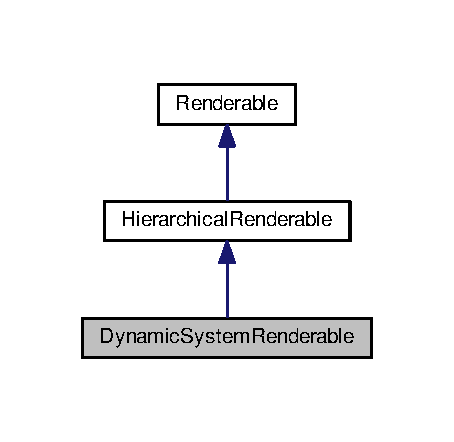
\includegraphics[width=218pt]{classDynamicSystemRenderable__inherit__graph}
\end{center}
\end{figure}


Collaboration diagram for Dynamic\+System\+Renderable\+:\nopagebreak
\begin{figure}[H]
\begin{center}
\leavevmode
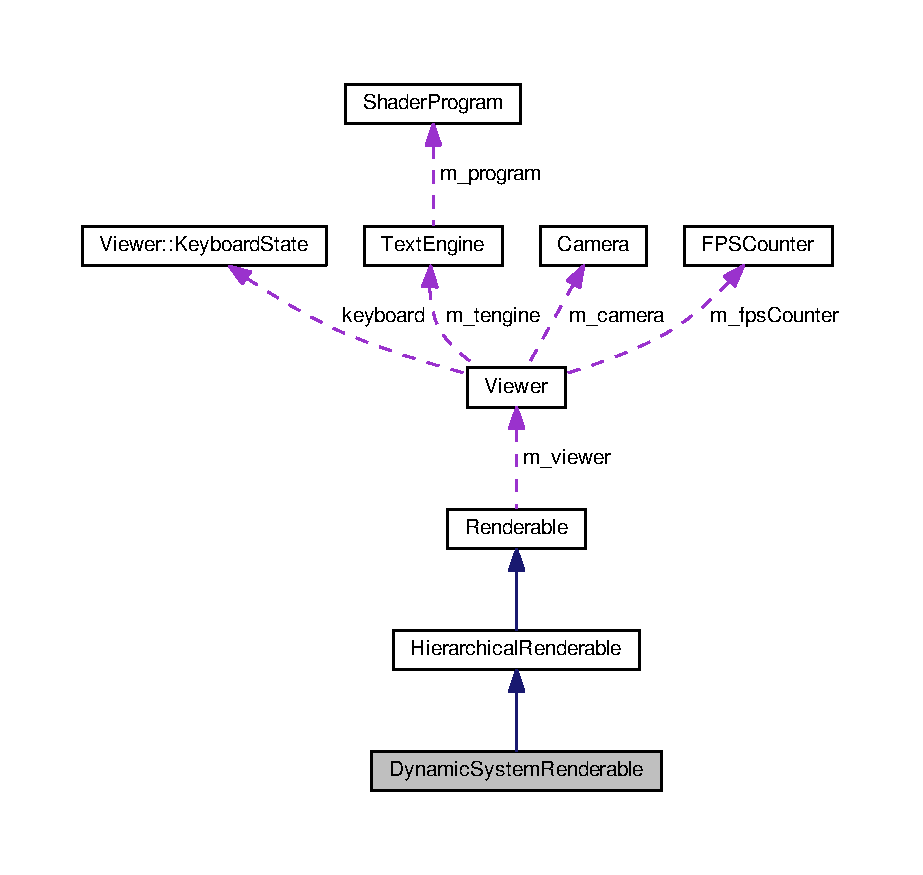
\includegraphics[width=350pt]{classDynamicSystemRenderable__coll__graph}
\end{center}
\end{figure}
\subsection*{Public Member Functions}
\begin{DoxyCompactItemize}
\item 
\hyperlink{classDynamicSystemRenderable_a9d6411c143db28c2d623928ac98f6aec}{$\sim$\+Dynamic\+System\+Renderable} ()
\item 
\hyperlink{classDynamicSystemRenderable_ab29cba8d5166e9cd636481e0bf284302}{Dynamic\+System\+Renderable} (\hyperlink{DynamicSystem_8hpp_a682a5f32e97dba69e8a4e542ed98b419}{Dynamic\+System\+Ptr} system)
\begin{DoxyCompactList}\small\item\em Build a dynamic system renderable. \end{DoxyCompactList}\item 
void \hyperlink{classDynamicSystemRenderable_a700986b9410c1d4a0a6ece669967b7c0}{set\+Dynamic\+System} (const \hyperlink{DynamicSystem_8hpp_a682a5f32e97dba69e8a4e542ed98b419}{Dynamic\+System\+Ptr} \&system)
\begin{DoxyCompactList}\small\item\em Change the managed dynamic system. \end{DoxyCompactList}\end{DoxyCompactItemize}
\subsection*{Private Member Functions}
\begin{DoxyCompactItemize}
\item 
void \hyperlink{classDynamicSystemRenderable_a8064176726a5d4b857a5e6a0fc73ff29}{do\+\_\+draw} ()
\begin{DoxyCompactList}\small\item\em Draw virtual function. \end{DoxyCompactList}\item 
void \hyperlink{classDynamicSystemRenderable_acd30af04cdca7cdc68ae2d49c179d2dc}{do\+\_\+animate} (float time)
\begin{DoxyCompactList}\small\item\em Update the dynamic system. \end{DoxyCompactList}\item 
void \hyperlink{classDynamicSystemRenderable_ac179f3ba1cc294589327e7cb569c50da}{do\+\_\+key\+Pressed\+Event} (sf\+::\+Event \&e)
\begin{DoxyCompactList}\small\item\em Handle key pressed. \end{DoxyCompactList}\item 
void \hyperlink{classDynamicSystemRenderable_ac074ccfc934f15607b4db103c2281a64}{do\+\_\+key\+Released\+Event} (sf\+::\+Event \&e)
\begin{DoxyCompactList}\small\item\em Transmit a key released event to children. \end{DoxyCompactList}\end{DoxyCompactItemize}
\subsection*{Private Attributes}
\begin{DoxyCompactItemize}
\item 
\hyperlink{DynamicSystem_8hpp_a682a5f32e97dba69e8a4e542ed98b419}{Dynamic\+System\+Ptr} \hyperlink{classDynamicSystemRenderable_a49be4db93a0d7e1122278c9d0dac43f2}{m\+\_\+system}
\begin{DoxyCompactList}\small\item\em Dynamic system managed by this renderable. \end{DoxyCompactList}\item 
float \hyperlink{classDynamicSystemRenderable_a4f1e45c9b781ffc21b63dcf211991d10}{m\+\_\+last\+Update\+Time}
\begin{DoxyCompactList}\small\item\em Last time the dynamic system was updated. \end{DoxyCompactList}\end{DoxyCompactItemize}
\subsection*{Additional Inherited Members}


\subsection{Detailed Description}
This class is mostly a hack we use to deal with the dynamic system components inside the framework. We could (should) do that differently, but this hack was considered to be simpler for the students to understand, since it reuse the concept of renderable. Moreover, since it is a hierarchical renderable, it is possible to define a dynamic system in a local frame and then use hierarchical geometric transformation to replace it correctly in the scene. 

\subsection{Constructor \& Destructor Documentation}
\hypertarget{classDynamicSystemRenderable_a9d6411c143db28c2d623928ac98f6aec}{\index{Dynamic\+System\+Renderable@{Dynamic\+System\+Renderable}!````~Dynamic\+System\+Renderable@{$\sim$\+Dynamic\+System\+Renderable}}
\index{````~Dynamic\+System\+Renderable@{$\sim$\+Dynamic\+System\+Renderable}!Dynamic\+System\+Renderable@{Dynamic\+System\+Renderable}}
\subsubsection[{$\sim$\+Dynamic\+System\+Renderable}]{\setlength{\rightskip}{0pt plus 5cm}Dynamic\+System\+Renderable\+::$\sim$\+Dynamic\+System\+Renderable (
\begin{DoxyParamCaption}
{}
\end{DoxyParamCaption}
)}}\label{classDynamicSystemRenderable_a9d6411c143db28c2d623928ac98f6aec}
\hypertarget{classDynamicSystemRenderable_ab29cba8d5166e9cd636481e0bf284302}{\index{Dynamic\+System\+Renderable@{Dynamic\+System\+Renderable}!Dynamic\+System\+Renderable@{Dynamic\+System\+Renderable}}
\index{Dynamic\+System\+Renderable@{Dynamic\+System\+Renderable}!Dynamic\+System\+Renderable@{Dynamic\+System\+Renderable}}
\subsubsection[{Dynamic\+System\+Renderable}]{\setlength{\rightskip}{0pt plus 5cm}Dynamic\+System\+Renderable\+::\+Dynamic\+System\+Renderable (
\begin{DoxyParamCaption}
\item[{{\bf Dynamic\+System\+Ptr}}]{system}
\end{DoxyParamCaption}
)}}\label{classDynamicSystemRenderable_ab29cba8d5166e9cd636481e0bf284302}
Build a dynamic system renderable from a dynamic system. The dynamic system will them be updated by this renderable. It allows us also to interact with the dynamic system components thanks to user input events. 
\begin{DoxyParams}{Parameters}
{\em system} & The dynamic system to manage by this renderable. \\
\hline
\end{DoxyParams}


\subsection{Member Function Documentation}
\hypertarget{classDynamicSystemRenderable_acd30af04cdca7cdc68ae2d49c179d2dc}{\index{Dynamic\+System\+Renderable@{Dynamic\+System\+Renderable}!do\+\_\+animate@{do\+\_\+animate}}
\index{do\+\_\+animate@{do\+\_\+animate}!Dynamic\+System\+Renderable@{Dynamic\+System\+Renderable}}
\subsubsection[{do\+\_\+animate}]{\setlength{\rightskip}{0pt plus 5cm}void Dynamic\+System\+Renderable\+::do\+\_\+animate (
\begin{DoxyParamCaption}
\item[{float}]{time}
\end{DoxyParamCaption}
)\hspace{0.3cm}{\ttfamily [private]}, {\ttfamily [virtual]}}}\label{classDynamicSystemRenderable_acd30af04cdca7cdc68ae2d49c179d2dc}
This function will update the managed dynamic system, i.\+e. compute the new positions and velocities of the particles. This update will be actually done only if the last time the system was updated was more than m\+\_\+sytem-\/$>$m\+\_\+dt ago. This allows us to update the dynamic system at the specified time interval. 

Implements \hyperlink{classRenderable_aa5206322555c9dece40b21e797629b34}{Renderable}.

\hypertarget{classDynamicSystemRenderable_a8064176726a5d4b857a5e6a0fc73ff29}{\index{Dynamic\+System\+Renderable@{Dynamic\+System\+Renderable}!do\+\_\+draw@{do\+\_\+draw}}
\index{do\+\_\+draw@{do\+\_\+draw}!Dynamic\+System\+Renderable@{Dynamic\+System\+Renderable}}
\subsubsection[{do\+\_\+draw}]{\setlength{\rightskip}{0pt plus 5cm}void Dynamic\+System\+Renderable\+::do\+\_\+draw (
\begin{DoxyParamCaption}
{}
\end{DoxyParamCaption}
)\hspace{0.3cm}{\ttfamily [private]}, {\ttfamily [virtual]}}}\label{classDynamicSystemRenderable_a8064176726a5d4b857a5e6a0fc73ff29}
Implementation to draw this renderable. 

Implements \hyperlink{classRenderable_a98ab6308c1d2b56dacda7c435fb38d5b}{Renderable}.

\hypertarget{classDynamicSystemRenderable_ac179f3ba1cc294589327e7cb569c50da}{\index{Dynamic\+System\+Renderable@{Dynamic\+System\+Renderable}!do\+\_\+key\+Pressed\+Event@{do\+\_\+key\+Pressed\+Event}}
\index{do\+\_\+key\+Pressed\+Event@{do\+\_\+key\+Pressed\+Event}!Dynamic\+System\+Renderable@{Dynamic\+System\+Renderable}}
\subsubsection[{do\+\_\+key\+Pressed\+Event}]{\setlength{\rightskip}{0pt plus 5cm}void Dynamic\+System\+Renderable\+::do\+\_\+key\+Pressed\+Event (
\begin{DoxyParamCaption}
\item[{sf\+::\+Event \&}]{e}
\end{DoxyParamCaption}
)\hspace{0.3cm}{\ttfamily [private]}, {\ttfamily [virtual]}}}\label{classDynamicSystemRenderable_ac179f3ba1cc294589327e7cb569c50da}
If the key A is pressed, the collision detected is toggled. If the key T is pressed, particles are titled in random directions. If the key F5 is pressed, the particles are restarted. Other key pressed are transmitted to the children of this renderable. 
\begin{DoxyParams}{Parameters}
{\em e} & A key pressed event. \\
\hline
\end{DoxyParams}


Reimplemented from \hyperlink{classRenderable_a49e39be950dca7a925b8b79c13241e6b}{Renderable}.

\hypertarget{classDynamicSystemRenderable_ac074ccfc934f15607b4db103c2281a64}{\index{Dynamic\+System\+Renderable@{Dynamic\+System\+Renderable}!do\+\_\+key\+Released\+Event@{do\+\_\+key\+Released\+Event}}
\index{do\+\_\+key\+Released\+Event@{do\+\_\+key\+Released\+Event}!Dynamic\+System\+Renderable@{Dynamic\+System\+Renderable}}
\subsubsection[{do\+\_\+key\+Released\+Event}]{\setlength{\rightskip}{0pt plus 5cm}void Dynamic\+System\+Renderable\+::do\+\_\+key\+Released\+Event (
\begin{DoxyParamCaption}
\item[{sf\+::\+Event \&}]{e}
\end{DoxyParamCaption}
)\hspace{0.3cm}{\ttfamily [private]}, {\ttfamily [virtual]}}}\label{classDynamicSystemRenderable_ac074ccfc934f15607b4db103c2281a64}
Transmit a key released event to the children of this renderable. 

Reimplemented from \hyperlink{classRenderable_a89d4bacd849c3606529f92c44b0a3bc1}{Renderable}.

\hypertarget{classDynamicSystemRenderable_a700986b9410c1d4a0a6ece669967b7c0}{\index{Dynamic\+System\+Renderable@{Dynamic\+System\+Renderable}!set\+Dynamic\+System@{set\+Dynamic\+System}}
\index{set\+Dynamic\+System@{set\+Dynamic\+System}!Dynamic\+System\+Renderable@{Dynamic\+System\+Renderable}}
\subsubsection[{set\+Dynamic\+System}]{\setlength{\rightskip}{0pt plus 5cm}void Dynamic\+System\+Renderable\+::set\+Dynamic\+System (
\begin{DoxyParamCaption}
\item[{const {\bf Dynamic\+System\+Ptr} \&}]{system}
\end{DoxyParamCaption}
)}}\label{classDynamicSystemRenderable_a700986b9410c1d4a0a6ece669967b7c0}
Change the dynamic system that will be managed by this renderable. 
\begin{DoxyParams}{Parameters}
{\em system} & The new dynamic system managed by this. \\
\hline
\end{DoxyParams}


\subsection{Member Data Documentation}
\hypertarget{classDynamicSystemRenderable_a4f1e45c9b781ffc21b63dcf211991d10}{\index{Dynamic\+System\+Renderable@{Dynamic\+System\+Renderable}!m\+\_\+last\+Update\+Time@{m\+\_\+last\+Update\+Time}}
\index{m\+\_\+last\+Update\+Time@{m\+\_\+last\+Update\+Time}!Dynamic\+System\+Renderable@{Dynamic\+System\+Renderable}}
\subsubsection[{m\+\_\+last\+Update\+Time}]{\setlength{\rightskip}{0pt plus 5cm}float Dynamic\+System\+Renderable\+::m\+\_\+last\+Update\+Time\hspace{0.3cm}{\ttfamily [private]}}}\label{classDynamicSystemRenderable_a4f1e45c9b781ffc21b63dcf211991d10}
Store the last time the dynamic system was updated. This is used to keep updating the dynamic system at the specified time interval. \hypertarget{classDynamicSystemRenderable_a49be4db93a0d7e1122278c9d0dac43f2}{\index{Dynamic\+System\+Renderable@{Dynamic\+System\+Renderable}!m\+\_\+system@{m\+\_\+system}}
\index{m\+\_\+system@{m\+\_\+system}!Dynamic\+System\+Renderable@{Dynamic\+System\+Renderable}}
\subsubsection[{m\+\_\+system}]{\setlength{\rightskip}{0pt plus 5cm}{\bf Dynamic\+System\+Ptr} Dynamic\+System\+Renderable\+::m\+\_\+system\hspace{0.3cm}{\ttfamily [private]}}}\label{classDynamicSystemRenderable_a49be4db93a0d7e1122278c9d0dac43f2}
The dynamic system that is managed by this renderable, to compute the simulation steps and to handle use input events. 

The documentation for this class was generated from the following file\+:\begin{DoxyCompactItemize}
\item 
/home/chardon/\+Depot/ensimag/2\+A\+\_\+\+G3\+D/practicals/teacher\+Source/include/dynamics/\hyperlink{DynamicSystemRenderable_8hpp}{Dynamic\+System\+Renderable.\+hpp}\end{DoxyCompactItemize}

\hypertarget{classEulerExplicitSolver}{\section{Euler\+Explicit\+Solver Class Reference}
\label{classEulerExplicitSolver}\index{Euler\+Explicit\+Solver@{Euler\+Explicit\+Solver}}
}


Explicit Euler solver.  




{\ttfamily \#include $<$Euler\+Explicit\+Solver.\+hpp$>$}



Inheritance diagram for Euler\+Explicit\+Solver\+:\nopagebreak
\begin{figure}[H]
\begin{center}
\leavevmode
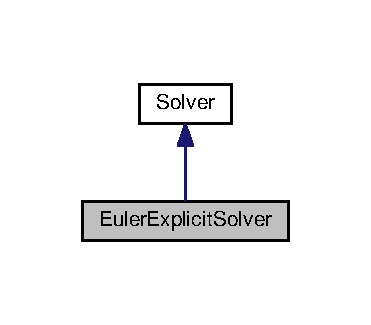
\includegraphics[width=178pt]{classEulerExplicitSolver__inherit__graph}
\end{center}
\end{figure}


Collaboration diagram for Euler\+Explicit\+Solver\+:\nopagebreak
\begin{figure}[H]
\begin{center}
\leavevmode
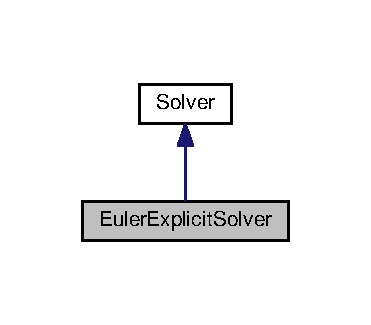
\includegraphics[width=178pt]{classEulerExplicitSolver__coll__graph}
\end{center}
\end{figure}
\subsection*{Public Member Functions}
\begin{DoxyCompactItemize}
\item 
\hyperlink{classEulerExplicitSolver_a6484746b2b67ee17597f63a5028df2fa}{Euler\+Explicit\+Solver} ()
\item 
\hyperlink{classEulerExplicitSolver_a84711eba5ad543c2a142f64d23de1bf6}{$\sim$\+Euler\+Explicit\+Solver} ()
\end{DoxyCompactItemize}
\subsection*{Private Member Functions}
\begin{DoxyCompactItemize}
\item 
void \hyperlink{classEulerExplicitSolver_aaaa3657876aff1c53a9a8a78c610757e}{do\+\_\+solve} (const float \&dt, std\+::vector$<$ \hyperlink{Particle_8hpp_a9a7abc8635002993537b61ef2c857fdd}{Particle\+Ptr} $>$ \&particles)
\begin{DoxyCompactList}\small\item\em Solve implementation. \end{DoxyCompactList}\end{DoxyCompactItemize}


\subsection{Detailed Description}
Explicit Euler dynamic system solver. 

\subsection{Constructor \& Destructor Documentation}
\hypertarget{classEulerExplicitSolver_a6484746b2b67ee17597f63a5028df2fa}{\index{Euler\+Explicit\+Solver@{Euler\+Explicit\+Solver}!Euler\+Explicit\+Solver@{Euler\+Explicit\+Solver}}
\index{Euler\+Explicit\+Solver@{Euler\+Explicit\+Solver}!Euler\+Explicit\+Solver@{Euler\+Explicit\+Solver}}
\subsubsection[{Euler\+Explicit\+Solver}]{\setlength{\rightskip}{0pt plus 5cm}Euler\+Explicit\+Solver\+::\+Euler\+Explicit\+Solver (
\begin{DoxyParamCaption}
{}
\end{DoxyParamCaption}
)}}\label{classEulerExplicitSolver_a6484746b2b67ee17597f63a5028df2fa}
\hypertarget{classEulerExplicitSolver_a84711eba5ad543c2a142f64d23de1bf6}{\index{Euler\+Explicit\+Solver@{Euler\+Explicit\+Solver}!````~Euler\+Explicit\+Solver@{$\sim$\+Euler\+Explicit\+Solver}}
\index{````~Euler\+Explicit\+Solver@{$\sim$\+Euler\+Explicit\+Solver}!Euler\+Explicit\+Solver@{Euler\+Explicit\+Solver}}
\subsubsection[{$\sim$\+Euler\+Explicit\+Solver}]{\setlength{\rightskip}{0pt plus 5cm}Euler\+Explicit\+Solver\+::$\sim$\+Euler\+Explicit\+Solver (
\begin{DoxyParamCaption}
{}
\end{DoxyParamCaption}
)}}\label{classEulerExplicitSolver_a84711eba5ad543c2a142f64d23de1bf6}


\subsection{Member Function Documentation}
\hypertarget{classEulerExplicitSolver_aaaa3657876aff1c53a9a8a78c610757e}{\index{Euler\+Explicit\+Solver@{Euler\+Explicit\+Solver}!do\+\_\+solve@{do\+\_\+solve}}
\index{do\+\_\+solve@{do\+\_\+solve}!Euler\+Explicit\+Solver@{Euler\+Explicit\+Solver}}
\subsubsection[{do\+\_\+solve}]{\setlength{\rightskip}{0pt plus 5cm}void Euler\+Explicit\+Solver\+::do\+\_\+solve (
\begin{DoxyParamCaption}
\item[{const float \&}]{dt, }
\item[{std\+::vector$<$ {\bf Particle\+Ptr} $>$ \&}]{particles}
\end{DoxyParamCaption}
)\hspace{0.3cm}{\ttfamily [private]}, {\ttfamily [virtual]}}}\label{classEulerExplicitSolver_aaaa3657876aff1c53a9a8a78c610757e}
The actual implementation to solve the dynamic system. This should be implemented in derived classes. 
\begin{DoxyParams}{Parameters}
{\em dt} & The time step for the integration. \\
\hline
{\em particles} & The collection of particles. \\
\hline
\end{DoxyParams}


Implements \hyperlink{classSolver_a4559f655c64c879fffd49557de27ab7d}{Solver}.



The documentation for this class was generated from the following file\+:\begin{DoxyCompactItemize}
\item 
/home/chardon/\+Depot/ensimag/2\+A\+\_\+\+G3\+D/practicals/teacher\+Source/include/dynamics/\hyperlink{EulerExplicitSolver_8hpp}{Euler\+Explicit\+Solver.\+hpp}\end{DoxyCompactItemize}

\hypertarget{classForceField}{\section{Force\+Field Class Reference}
\label{classForceField}\index{Force\+Field@{Force\+Field}}
}


Force field interface.  




{\ttfamily \#include $<$Force\+Field.\+hpp$>$}



Inheritance diagram for Force\+Field\+:\nopagebreak
\begin{figure}[H]
\begin{center}
\leavevmode
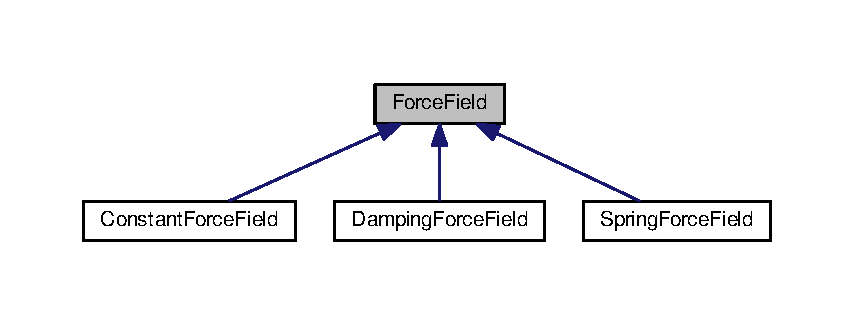
\includegraphics[width=350pt]{classForceField__inherit__graph}
\end{center}
\end{figure}
\subsection*{Public Member Functions}
\begin{DoxyCompactItemize}
\item 
\hyperlink{classForceField_a8273c2e8667bc21edb7599c1210dda4a}{Force\+Field} ()
\item 
virtual \hyperlink{classForceField_a718e3d630818c01519a99aa2088c0900}{$\sim$\+Force\+Field} ()
\item 
void \hyperlink{classForceField_acf0c3bb94b1a27adccab0835c49a47f1}{add\+Force} ()
\begin{DoxyCompactList}\small\item\em Add a force to particles. \end{DoxyCompactList}\end{DoxyCompactItemize}
\subsection*{Private Member Functions}
\begin{DoxyCompactItemize}
\item 
virtual void \hyperlink{classForceField_a2f44520a00188a3aaeb04e667e8d2673}{do\+\_\+add\+Force} ()=0
\begin{DoxyCompactList}\small\item\em Add force implementation. \end{DoxyCompactList}\end{DoxyCompactItemize}


\subsection{Detailed Description}
Define an interface for a force field. A force field applies forces to a set of handled particles. Those particles are stored in derived classes. 

\subsection{Constructor \& Destructor Documentation}
\hypertarget{classForceField_a8273c2e8667bc21edb7599c1210dda4a}{\index{Force\+Field@{Force\+Field}!Force\+Field@{Force\+Field}}
\index{Force\+Field@{Force\+Field}!Force\+Field@{Force\+Field}}
\subsubsection[{Force\+Field}]{\setlength{\rightskip}{0pt plus 5cm}Force\+Field\+::\+Force\+Field (
\begin{DoxyParamCaption}
{}
\end{DoxyParamCaption}
)}}\label{classForceField_a8273c2e8667bc21edb7599c1210dda4a}
\hypertarget{classForceField_a718e3d630818c01519a99aa2088c0900}{\index{Force\+Field@{Force\+Field}!````~Force\+Field@{$\sim$\+Force\+Field}}
\index{````~Force\+Field@{$\sim$\+Force\+Field}!Force\+Field@{Force\+Field}}
\subsubsection[{$\sim$\+Force\+Field}]{\setlength{\rightskip}{0pt plus 5cm}virtual Force\+Field\+::$\sim$\+Force\+Field (
\begin{DoxyParamCaption}
{}
\end{DoxyParamCaption}
)\hspace{0.3cm}{\ttfamily [virtual]}}}\label{classForceField_a718e3d630818c01519a99aa2088c0900}


\subsection{Member Function Documentation}
\hypertarget{classForceField_acf0c3bb94b1a27adccab0835c49a47f1}{\index{Force\+Field@{Force\+Field}!add\+Force@{add\+Force}}
\index{add\+Force@{add\+Force}!Force\+Field@{Force\+Field}}
\subsubsection[{add\+Force}]{\setlength{\rightskip}{0pt plus 5cm}void Force\+Field\+::add\+Force (
\begin{DoxyParamCaption}
{}
\end{DoxyParamCaption}
)}}\label{classForceField_acf0c3bb94b1a27adccab0835c49a47f1}
Add a force to the particles influenced by this force field. \hypertarget{classForceField_a2f44520a00188a3aaeb04e667e8d2673}{\index{Force\+Field@{Force\+Field}!do\+\_\+add\+Force@{do\+\_\+add\+Force}}
\index{do\+\_\+add\+Force@{do\+\_\+add\+Force}!Force\+Field@{Force\+Field}}
\subsubsection[{do\+\_\+add\+Force}]{\setlength{\rightskip}{0pt plus 5cm}virtual void Force\+Field\+::do\+\_\+add\+Force (
\begin{DoxyParamCaption}
{}
\end{DoxyParamCaption}
)\hspace{0.3cm}{\ttfamily [private]}, {\ttfamily [pure virtual]}}}\label{classForceField_a2f44520a00188a3aaeb04e667e8d2673}
The actual implementation to add force to the particles. This should be implemented in derived classes. 

Implemented in \hyperlink{classConstantForceField_a4336bdbfa85ac10cc8a50170ab515061}{Constant\+Force\+Field}, \hyperlink{classDampingForceField_a5677c09b83f6f2d13e70e40c08c4e85f}{Damping\+Force\+Field}, and \hyperlink{classSpringForceField_a09e9e100a1947a43fdc1c9487d72a08e}{Spring\+Force\+Field}.



The documentation for this class was generated from the following file\+:\begin{DoxyCompactItemize}
\item 
/home/chardon/\+Depot/ensimag/2\+A\+\_\+\+G3\+D/practicals/teacher\+Source/include/dynamics/\hyperlink{ForceField_8hpp}{Force\+Field.\+hpp}\end{DoxyCompactItemize}

\hypertarget{classFPSCounter}{\section{F\+P\+S\+Counter Class Reference}
\label{classFPSCounter}\index{F\+P\+S\+Counter@{F\+P\+S\+Counter}}
}


Compute an averaged F\+P\+S.  




{\ttfamily \#include $<$F\+P\+S\+Counter.\+hpp$>$}

\subsection*{Public Member Functions}
\begin{DoxyCompactItemize}
\item 
\hyperlink{classFPSCounter_a5302dd56ff08c75f086680163d410f57}{F\+P\+S\+Counter} (double refresh\+Interval=2.\+0)
\begin{DoxyCompactList}\small\item\em Build a F\+P\+S counter with a specific refresh interval. \end{DoxyCompactList}\item 
\hyperlink{classFPSCounter_acaa2539d1af5e6da509f5ce32b13972d}{$\sim$\+F\+P\+S\+Counter} ()
\begin{DoxyCompactList}\small\item\em Instance destructor. \end{DoxyCompactList}\item 
float \hyperlink{classFPSCounter_a2b7e118b610867e4f62b359eb589e65f}{get\+F\+P\+S} ()
\begin{DoxyCompactList}\small\item\em Get the averaged F\+P\+S count. \end{DoxyCompactList}\end{DoxyCompactItemize}
\subsection*{Private Types}
\begin{DoxyCompactItemize}
\item 
typedef std\+::chrono\+::system\+\_\+clock \hyperlink{classFPSCounter_aff42afc3b6d4fd2b4fcdb7579fa48031}{clock}
\item 
typedef std\+::chrono\+::duration\\*
$<$ double $>$ \hyperlink{classFPSCounter_a2cb0edfdff687339a681ce0349febe4b}{Duration}
\item 
typedef \\*
std\+::chrono\+::time\+\_\+point$<$ \hyperlink{classFPSCounter_aff42afc3b6d4fd2b4fcdb7579fa48031}{clock}, \\*
\hyperlink{classFPSCounter_a2cb0edfdff687339a681ce0349febe4b}{Duration} $>$ \hyperlink{classFPSCounter_abdab5df998311505d5b39210eb4e4940}{Time\+Point}
\end{DoxyCompactItemize}
\subsection*{Private Attributes}
\begin{DoxyCompactItemize}
\item 
\hyperlink{classFPSCounter_a2cb0edfdff687339a681ce0349febe4b}{Duration} \hyperlink{classFPSCounter_a419142db73c011e326309be159419796}{m\+\_\+refresh\+Interval}
\item 
\hyperlink{classFPSCounter_abdab5df998311505d5b39210eb4e4940}{Time\+Point} \hyperlink{classFPSCounter_a1e88f7c01b50ddb5b113ed6cc95335bb}{m\+\_\+last\+Refresh\+Time}
\item 
\hyperlink{classFPSCounter_abdab5df998311505d5b39210eb4e4940}{Time\+Point} \hyperlink{classFPSCounter_a2571dd4fcfa2e6adeeca59088a3481cf}{m\+\_\+last\+Call\+Time}
\item 
double \hyperlink{classFPSCounter_a73c8cd4484bc8d851854f438aca5a2d4}{m\+\_\+accumulated\+F\+P\+S}
\item 
float \hyperlink{classFPSCounter_a29bfe52f7ae0f66958aab30e268e95ed}{m\+\_\+fps}
\item 
unsigned int \hyperlink{classFPSCounter_af985f96020619ec9c94dc1d059f4512d}{m\+\_\+number\+Of\+Samples}
\end{DoxyCompactItemize}


\subsection{Detailed Description}
This helper class provides an automatically updated and averaged F\+P\+S count. The value is averaged at each interval specified in the constructor. A typical use of this class\+: 
\begin{DoxyCode}
\hyperlink{classFPSCounter}{FPSCounter} counter( 1.5 ); \textcolor{comment}{// value refreshed every 1.5 second}
\textcolor{keywordflow}{while}( running ) \textcolor{comment}{// main rendering loop}
\{
  \textcolor{keywordtype}{float} averageFPS = counter.getFPS();
  \textcolor{comment}{// averageFPS is guaranteed to remain the same for each interval}
  \textcolor{comment}{// of 1.5 second. We can then display this value on screen: it will}
  \textcolor{comment}{// slowly change such that we can still read it correctly.}
\}
\end{DoxyCode}
 

\subsection{Member Typedef Documentation}
\hypertarget{classFPSCounter_aff42afc3b6d4fd2b4fcdb7579fa48031}{\index{F\+P\+S\+Counter@{F\+P\+S\+Counter}!clock@{clock}}
\index{clock@{clock}!F\+P\+S\+Counter@{F\+P\+S\+Counter}}
\subsubsection[{clock}]{\setlength{\rightskip}{0pt plus 5cm}typedef std\+::chrono\+::system\+\_\+clock {\bf F\+P\+S\+Counter\+::clock}\hspace{0.3cm}{\ttfamily [private]}}}\label{classFPSCounter_aff42afc3b6d4fd2b4fcdb7579fa48031}
We use the system\+\_\+clock of std\+::chrono to compute durations. chrono is a nice addition to the c++ std, go have a look there\+: \href{http://www.cplusplus.com/reference/chrono/}{\tt http\+://www.\+cplusplus.\+com/reference/chrono/} \hypertarget{classFPSCounter_a2cb0edfdff687339a681ce0349febe4b}{\index{F\+P\+S\+Counter@{F\+P\+S\+Counter}!Duration@{Duration}}
\index{Duration@{Duration}!F\+P\+S\+Counter@{F\+P\+S\+Counter}}
\subsubsection[{Duration}]{\setlength{\rightskip}{0pt plus 5cm}typedef std\+::chrono\+::duration$<$double$>$ {\bf F\+P\+S\+Counter\+::\+Duration}\hspace{0.3cm}{\ttfamily [private]}}}\label{classFPSCounter_a2cb0edfdff687339a681ce0349febe4b}
We use a double precision duration type to have a precise F\+P\+S estimation. \hypertarget{classFPSCounter_abdab5df998311505d5b39210eb4e4940}{\index{F\+P\+S\+Counter@{F\+P\+S\+Counter}!Time\+Point@{Time\+Point}}
\index{Time\+Point@{Time\+Point}!F\+P\+S\+Counter@{F\+P\+S\+Counter}}
\subsubsection[{Time\+Point}]{\setlength{\rightskip}{0pt plus 5cm}typedef std\+::chrono\+::time\+\_\+point$<$ {\bf clock}, {\bf Duration} $>$ {\bf F\+P\+S\+Counter\+::\+Time\+Point}\hspace{0.3cm}{\ttfamily [private]}}}\label{classFPSCounter_abdab5df998311505d5b39210eb4e4940}
Based on the clock and the duration types, we define a time point type to store last events date. 

\subsection{Constructor \& Destructor Documentation}
\hypertarget{classFPSCounter_a5302dd56ff08c75f086680163d410f57}{\index{F\+P\+S\+Counter@{F\+P\+S\+Counter}!F\+P\+S\+Counter@{F\+P\+S\+Counter}}
\index{F\+P\+S\+Counter@{F\+P\+S\+Counter}!F\+P\+S\+Counter@{F\+P\+S\+Counter}}
\subsubsection[{F\+P\+S\+Counter}]{\setlength{\rightskip}{0pt plus 5cm}F\+P\+S\+Counter\+::\+F\+P\+S\+Counter (
\begin{DoxyParamCaption}
\item[{double}]{refresh\+Interval = {\ttfamily 2.0}}
\end{DoxyParamCaption}
)}}\label{classFPSCounter_a5302dd56ff08c75f086680163d410f57}
Create a F\+P\+S counter that will be refreshed every display\+Interval second(s).


\begin{DoxyParams}{Parameters}
{\em refresh\+Interval} & refresh interval, i.\+e. minimum duration for which the value returned by this won't change. At the end of the interval, a new F\+P\+S value is computed and stored to be returned. \\
\hline
\end{DoxyParams}
\hypertarget{classFPSCounter_acaa2539d1af5e6da509f5ce32b13972d}{\index{F\+P\+S\+Counter@{F\+P\+S\+Counter}!````~F\+P\+S\+Counter@{$\sim$\+F\+P\+S\+Counter}}
\index{````~F\+P\+S\+Counter@{$\sim$\+F\+P\+S\+Counter}!F\+P\+S\+Counter@{F\+P\+S\+Counter}}
\subsubsection[{$\sim$\+F\+P\+S\+Counter}]{\setlength{\rightskip}{0pt plus 5cm}F\+P\+S\+Counter\+::$\sim$\+F\+P\+S\+Counter (
\begin{DoxyParamCaption}
{}
\end{DoxyParamCaption}
)}}\label{classFPSCounter_acaa2539d1af5e6da509f5ce32b13972d}
Instance destructor. 

\subsection{Member Function Documentation}
\hypertarget{classFPSCounter_a2b7e118b610867e4f62b359eb589e65f}{\index{F\+P\+S\+Counter@{F\+P\+S\+Counter}!get\+F\+P\+S@{get\+F\+P\+S}}
\index{get\+F\+P\+S@{get\+F\+P\+S}!F\+P\+S\+Counter@{F\+P\+S\+Counter}}
\subsubsection[{get\+F\+P\+S}]{\setlength{\rightskip}{0pt plus 5cm}float F\+P\+S\+Counter\+::get\+F\+P\+S (
\begin{DoxyParamCaption}
{}
\end{DoxyParamCaption}
)}}\label{classFPSCounter_a2b7e118b610867e4f62b359eb589e65f}
This function updates the internal members of the instance, taking into account the last time it was called. If the last refresh was enough time ago, a new averaged fps count is computed. This is this averaged fps count that is returned in all cases.

\begin{DoxyReturn}{Returns}
The averaged F\+P\+S count. 
\end{DoxyReturn}


\subsection{Member Data Documentation}
\hypertarget{classFPSCounter_a73c8cd4484bc8d851854f438aca5a2d4}{\index{F\+P\+S\+Counter@{F\+P\+S\+Counter}!m\+\_\+accumulated\+F\+P\+S@{m\+\_\+accumulated\+F\+P\+S}}
\index{m\+\_\+accumulated\+F\+P\+S@{m\+\_\+accumulated\+F\+P\+S}!F\+P\+S\+Counter@{F\+P\+S\+Counter}}
\subsubsection[{m\+\_\+accumulated\+F\+P\+S}]{\setlength{\rightskip}{0pt plus 5cm}double F\+P\+S\+Counter\+::m\+\_\+accumulated\+F\+P\+S\hspace{0.3cm}{\ttfamily [private]}}}\label{classFPSCounter_a73c8cd4484bc8d851854f438aca5a2d4}
The sum of the F\+P\+S computed at each call to \hyperlink{classFPSCounter_a2b7e118b610867e4f62b359eb589e65f}{get\+F\+P\+S()} since last refresh. \hypertarget{classFPSCounter_a29bfe52f7ae0f66958aab30e268e95ed}{\index{F\+P\+S\+Counter@{F\+P\+S\+Counter}!m\+\_\+fps@{m\+\_\+fps}}
\index{m\+\_\+fps@{m\+\_\+fps}!F\+P\+S\+Counter@{F\+P\+S\+Counter}}
\subsubsection[{m\+\_\+fps}]{\setlength{\rightskip}{0pt plus 5cm}float F\+P\+S\+Counter\+::m\+\_\+fps\hspace{0.3cm}{\ttfamily [private]}}}\label{classFPSCounter_a29bfe52f7ae0f66958aab30e268e95ed}
Averaged F\+P\+S count stored such that \hyperlink{classFPSCounter_a2b7e118b610867e4f62b359eb589e65f}{get\+F\+P\+S()} returns the same value between two refreshes. When a refresh occurs, this value receives \hyperlink{classFPSCounter_a73c8cd4484bc8d851854f438aca5a2d4}{F\+P\+S\+Counter\+::m\+\_\+accumulated\+F\+P\+S} / \hyperlink{classFPSCounter_af985f96020619ec9c94dc1d059f4512d}{F\+P\+S\+Counter\+::m\+\_\+number\+Of\+Samples}. \hypertarget{classFPSCounter_a2571dd4fcfa2e6adeeca59088a3481cf}{\index{F\+P\+S\+Counter@{F\+P\+S\+Counter}!m\+\_\+last\+Call\+Time@{m\+\_\+last\+Call\+Time}}
\index{m\+\_\+last\+Call\+Time@{m\+\_\+last\+Call\+Time}!F\+P\+S\+Counter@{F\+P\+S\+Counter}}
\subsubsection[{m\+\_\+last\+Call\+Time}]{\setlength{\rightskip}{0pt plus 5cm}{\bf Time\+Point} F\+P\+S\+Counter\+::m\+\_\+last\+Call\+Time\hspace{0.3cm}{\ttfamily [private]}}}\label{classFPSCounter_a2571dd4fcfa2e6adeeca59088a3481cf}
Last time \hyperlink{classFPSCounter_a2b7e118b610867e4f62b359eb589e65f}{get\+F\+P\+S()} was called. \hypertarget{classFPSCounter_a1e88f7c01b50ddb5b113ed6cc95335bb}{\index{F\+P\+S\+Counter@{F\+P\+S\+Counter}!m\+\_\+last\+Refresh\+Time@{m\+\_\+last\+Refresh\+Time}}
\index{m\+\_\+last\+Refresh\+Time@{m\+\_\+last\+Refresh\+Time}!F\+P\+S\+Counter@{F\+P\+S\+Counter}}
\subsubsection[{m\+\_\+last\+Refresh\+Time}]{\setlength{\rightskip}{0pt plus 5cm}{\bf Time\+Point} F\+P\+S\+Counter\+::m\+\_\+last\+Refresh\+Time\hspace{0.3cm}{\ttfamily [private]}}}\label{classFPSCounter_a1e88f7c01b50ddb5b113ed6cc95335bb}
Last time the \hyperlink{classFPSCounter_a29bfe52f7ae0f66958aab30e268e95ed}{F\+P\+S\+Counter\+::m\+\_\+fps} was refreshed. \hypertarget{classFPSCounter_af985f96020619ec9c94dc1d059f4512d}{\index{F\+P\+S\+Counter@{F\+P\+S\+Counter}!m\+\_\+number\+Of\+Samples@{m\+\_\+number\+Of\+Samples}}
\index{m\+\_\+number\+Of\+Samples@{m\+\_\+number\+Of\+Samples}!F\+P\+S\+Counter@{F\+P\+S\+Counter}}
\subsubsection[{m\+\_\+number\+Of\+Samples}]{\setlength{\rightskip}{0pt plus 5cm}unsigned int F\+P\+S\+Counter\+::m\+\_\+number\+Of\+Samples\hspace{0.3cm}{\ttfamily [private]}}}\label{classFPSCounter_af985f96020619ec9c94dc1d059f4512d}
The number of F\+P\+S computed by each call to \hyperlink{classFPSCounter_a2b7e118b610867e4f62b359eb589e65f}{get\+F\+P\+S()} since last refresh. \hypertarget{classFPSCounter_a419142db73c011e326309be159419796}{\index{F\+P\+S\+Counter@{F\+P\+S\+Counter}!m\+\_\+refresh\+Interval@{m\+\_\+refresh\+Interval}}
\index{m\+\_\+refresh\+Interval@{m\+\_\+refresh\+Interval}!F\+P\+S\+Counter@{F\+P\+S\+Counter}}
\subsubsection[{m\+\_\+refresh\+Interval}]{\setlength{\rightskip}{0pt plus 5cm}{\bf Duration} F\+P\+S\+Counter\+::m\+\_\+refresh\+Interval\hspace{0.3cm}{\ttfamily [private]}}}\label{classFPSCounter_a419142db73c011e326309be159419796}
Duration between two refresh of \hyperlink{classFPSCounter_a29bfe52f7ae0f66958aab30e268e95ed}{F\+P\+S\+Counter\+::m\+\_\+fps}. 

The documentation for this class was generated from the following file\+:\begin{DoxyCompactItemize}
\item 
/home/chardon/\+Depot/ensimag/2\+A\+\_\+\+G3\+D/practicals/teacher\+Source/include/\hyperlink{FPSCounter_8hpp}{F\+P\+S\+Counter.\+hpp}\end{DoxyCompactItemize}

\hypertarget{classFrameRenderable}{\section{Frame\+Renderable Class Reference}
\label{classFrameRenderable}\index{Frame\+Renderable@{Frame\+Renderable}}
}


Render the world frame.  




{\ttfamily \#include $<$Frame\+Renderable.\+hpp$>$}



Inheritance diagram for Frame\+Renderable\+:\nopagebreak
\begin{figure}[H]
\begin{center}
\leavevmode
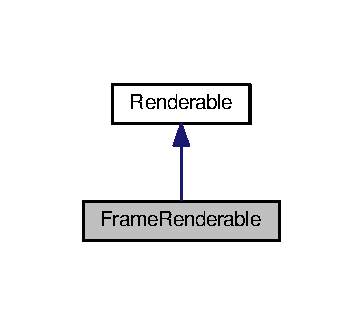
\includegraphics[width=174pt]{classFrameRenderable__inherit__graph}
\end{center}
\end{figure}


Collaboration diagram for Frame\+Renderable\+:\nopagebreak
\begin{figure}[H]
\begin{center}
\leavevmode
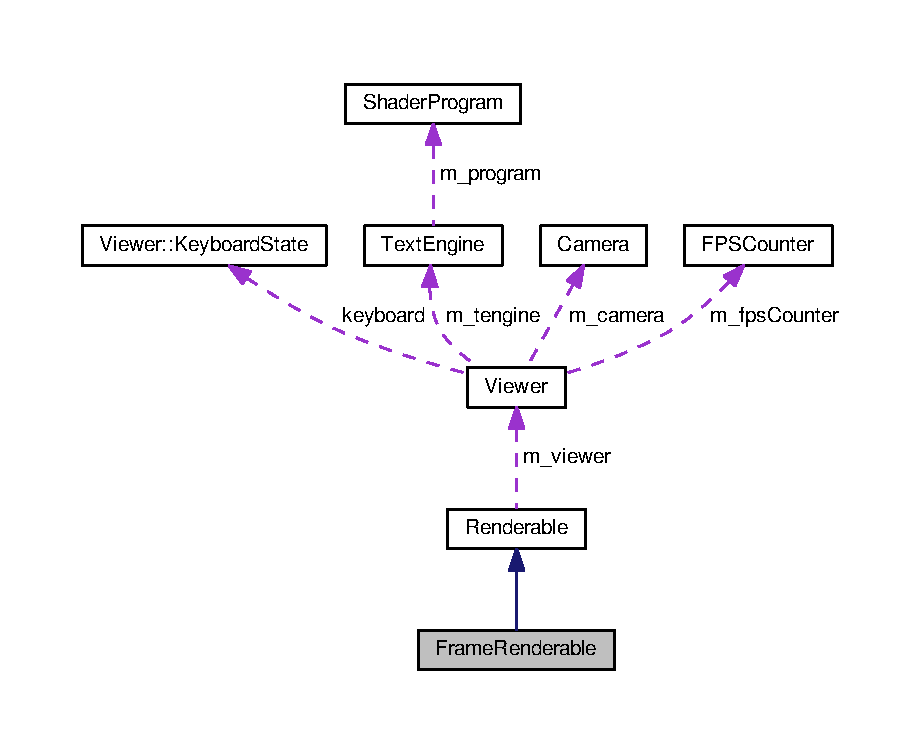
\includegraphics[width=350pt]{classFrameRenderable__coll__graph}
\end{center}
\end{figure}
\subsection*{Public Member Functions}
\begin{DoxyCompactItemize}
\item 
\hyperlink{classFrameRenderable_a823e77f15071737444f4bc7e589ca842}{$\sim$\+Frame\+Renderable} ()
\begin{DoxyCompactList}\small\item\em Destructor. \end{DoxyCompactList}\item 
\hyperlink{classFrameRenderable_a6d63f3eb741826c84fb49db9887efd3b}{Frame\+Renderable} (\hyperlink{ShaderProgram_8hpp_af8e4af1ad4c53875ee5d32ab7e1f4966}{Shader\+Program\+Ptr} shader\+Program)
\begin{DoxyCompactList}\small\item\em Constructor. \end{DoxyCompactList}\end{DoxyCompactItemize}
\subsection*{Private Member Functions}
\begin{DoxyCompactItemize}
\item 
\hyperlink{classFrameRenderable_a5984573fc1ac50ce3c0761f6e7ba78e1}{Frame\+Renderable} ()
\begin{DoxyCompactList}\small\item\em Forbidden default constructor. \end{DoxyCompactList}\item 
void \hyperlink{classFrameRenderable_aafa6b6444c8fa20a177eb562ba1a2672}{do\+\_\+draw} ()
\begin{DoxyCompactList}\small\item\em Draw this renderable. \end{DoxyCompactList}\item 
void \hyperlink{classFrameRenderable_a331b31de3a4988acf6304c30762d99cc}{do\+\_\+animate} (float time)
\begin{DoxyCompactList}\small\item\em Animate this renderable. \end{DoxyCompactList}\item 
void \hyperlink{classFrameRenderable_a39c514efa0139273930784ffec8329e9}{init\+Attributes} ()
\begin{DoxyCompactList}\small\item\em Initialize the vertex attributes of the frame. \end{DoxyCompactList}\end{DoxyCompactItemize}
\subsection*{Private Attributes}
\begin{DoxyCompactItemize}
\item 
std\+::vector$<$ glm\+::vec3 $>$ \hyperlink{classFrameRenderable_a6cb58f4ca3a0198e628da450f2a4c731}{m\+\_\+positions}
\begin{DoxyCompactList}\small\item\em Position attribute of the vertices. \end{DoxyCompactList}\item 
std\+::vector$<$ glm\+::vec4 $>$ \hyperlink{classFrameRenderable_a95e44e90b8e1f1ac67967003aea63009}{m\+\_\+colors}
\item 
unsigned int \hyperlink{classFrameRenderable_a89c0e4abd391a47198729001a2d5f159}{m\+\_\+p\+Buffer}
\begin{DoxyCompactList}\small\item\em Location of the position attribute buffer. \end{DoxyCompactList}\item 
unsigned int \hyperlink{classFrameRenderable_a6c8bed148c506c1a26fd7fc3cc5c625a}{m\+\_\+c\+Buffer}
\begin{DoxyCompactList}\small\item\em Location of the color attribute buffer. \end{DoxyCompactList}\end{DoxyCompactItemize}
\subsection*{Additional Inherited Members}


\subsection{Detailed Description}
This class is the first renderable you will use (see the Tutorial 03 of practical 01). It will render the world frame on the screen\+: a red line for the X axis, a green line for the Y axis and a blue line for the Z axis. Have a look at the source\+: we documented it to help you to understand the details. 

\subsection{Constructor \& Destructor Documentation}
\hypertarget{classFrameRenderable_a823e77f15071737444f4bc7e589ca842}{\index{Frame\+Renderable@{Frame\+Renderable}!````~Frame\+Renderable@{$\sim$\+Frame\+Renderable}}
\index{````~Frame\+Renderable@{$\sim$\+Frame\+Renderable}!Frame\+Renderable@{Frame\+Renderable}}
\subsubsection[{$\sim$\+Frame\+Renderable}]{\setlength{\rightskip}{0pt plus 5cm}Frame\+Renderable\+::$\sim$\+Frame\+Renderable (
\begin{DoxyParamCaption}
{}
\end{DoxyParamCaption}
)}}\label{classFrameRenderable_a823e77f15071737444f4bc7e589ca842}
Instance destructor. \hypertarget{classFrameRenderable_a6d63f3eb741826c84fb49db9887efd3b}{\index{Frame\+Renderable@{Frame\+Renderable}!Frame\+Renderable@{Frame\+Renderable}}
\index{Frame\+Renderable@{Frame\+Renderable}!Frame\+Renderable@{Frame\+Renderable}}
\subsubsection[{Frame\+Renderable}]{\setlength{\rightskip}{0pt plus 5cm}Frame\+Renderable\+::\+Frame\+Renderable (
\begin{DoxyParamCaption}
\item[{{\bf Shader\+Program\+Ptr}}]{shader\+Program}
\end{DoxyParamCaption}
)}}\label{classFrameRenderable_a6d63f3eb741826c84fb49db9887efd3b}
Create a new instance that will rendered thanks to the given shader program. 
\begin{DoxyParams}{Parameters}
{\em shader\+Program} & The shader program to use to render this frame renderable. \\
\hline
\end{DoxyParams}
\hypertarget{classFrameRenderable_a5984573fc1ac50ce3c0761f6e7ba78e1}{\index{Frame\+Renderable@{Frame\+Renderable}!Frame\+Renderable@{Frame\+Renderable}}
\index{Frame\+Renderable@{Frame\+Renderable}!Frame\+Renderable@{Frame\+Renderable}}
\subsubsection[{Frame\+Renderable}]{\setlength{\rightskip}{0pt plus 5cm}Frame\+Renderable\+::\+Frame\+Renderable (
\begin{DoxyParamCaption}
{}
\end{DoxyParamCaption}
)\hspace{0.3cm}{\ttfamily [private]}}}\label{classFrameRenderable_a5984573fc1ac50ce3c0761f6e7ba78e1}
By putting the default constructor in the private section, we make it forbidden (since it is private, no other class can call it). We do not need to provide an implementation as the compiler will never need it. 

\subsection{Member Function Documentation}
\hypertarget{classFrameRenderable_a331b31de3a4988acf6304c30762d99cc}{\index{Frame\+Renderable@{Frame\+Renderable}!do\+\_\+animate@{do\+\_\+animate}}
\index{do\+\_\+animate@{do\+\_\+animate}!Frame\+Renderable@{Frame\+Renderable}}
\subsubsection[{do\+\_\+animate}]{\setlength{\rightskip}{0pt plus 5cm}void Frame\+Renderable\+::do\+\_\+animate (
\begin{DoxyParamCaption}
\item[{float}]{time}
\end{DoxyParamCaption}
)\hspace{0.3cm}{\ttfamily [private]}, {\ttfamily [virtual]}}}\label{classFrameRenderable_a331b31de3a4988acf6304c30762d99cc}
The implementation of the \hyperlink{classRenderable_a74fd37d6852fb727e1a5fe72541d269d}{animate( float time )} or \hyperlink{classRenderable}{Renderable}. This does nothing as we do not need to animate it. 
\begin{DoxyParams}{Parameters}
{\em time} & The current simulation time. \\
\hline
\end{DoxyParams}


Implements \hyperlink{classRenderable_aa5206322555c9dece40b21e797629b34}{Renderable}.

\hypertarget{classFrameRenderable_aafa6b6444c8fa20a177eb562ba1a2672}{\index{Frame\+Renderable@{Frame\+Renderable}!do\+\_\+draw@{do\+\_\+draw}}
\index{do\+\_\+draw@{do\+\_\+draw}!Frame\+Renderable@{Frame\+Renderable}}
\subsubsection[{do\+\_\+draw}]{\setlength{\rightskip}{0pt plus 5cm}void Frame\+Renderable\+::do\+\_\+draw (
\begin{DoxyParamCaption}
{}
\end{DoxyParamCaption}
)\hspace{0.3cm}{\ttfamily [private]}, {\ttfamily [virtual]}}}\label{classFrameRenderable_aafa6b6444c8fa20a177eb562ba1a2672}
The implementation of the \hyperlink{classRenderable_a0d371901a19b8cfe50b76b842adba70a}{draw()} interface of \hyperlink{classRenderable}{Renderable}. This is where drawing commands are issued. 

Implements \hyperlink{classRenderable_a98ab6308c1d2b56dacda7c435fb38d5b}{Renderable}.

\hypertarget{classFrameRenderable_a39c514efa0139273930784ffec8329e9}{\index{Frame\+Renderable@{Frame\+Renderable}!init\+Attributes@{init\+Attributes}}
\index{init\+Attributes@{init\+Attributes}!Frame\+Renderable@{Frame\+Renderable}}
\subsubsection[{init\+Attributes}]{\setlength{\rightskip}{0pt plus 5cm}void Frame\+Renderable\+::init\+Attributes (
\begin{DoxyParamCaption}
{}
\end{DoxyParamCaption}
)\hspace{0.3cm}{\ttfamily [private]}}}\label{classFrameRenderable_a39c514efa0139273930784ffec8329e9}
This function intializes the geometry and the color of the frame. We put it in its own method help you to understand what is done in the constructor. 

\subsection{Member Data Documentation}
\hypertarget{classFrameRenderable_a6c8bed148c506c1a26fd7fc3cc5c625a}{\index{Frame\+Renderable@{Frame\+Renderable}!m\+\_\+c\+Buffer@{m\+\_\+c\+Buffer}}
\index{m\+\_\+c\+Buffer@{m\+\_\+c\+Buffer}!Frame\+Renderable@{Frame\+Renderable}}
\subsubsection[{m\+\_\+c\+Buffer}]{\setlength{\rightskip}{0pt plus 5cm}unsigned int Frame\+Renderable\+::m\+\_\+c\+Buffer\hspace{0.3cm}{\ttfamily [private]}}}\label{classFrameRenderable_a6c8bed148c506c1a26fd7fc3cc5c625a}
Store the location (index) of the color attribute buffer on the shader program used to render the instance. If all instances are rendered by the same shader program, you could make this location static and set this location when the first instance is created. We decided to not make it static as it would be harder to understand and it is quite constraining\+: if you want to use more than shader program to render frame renderable instances, this will lead to bugs tricky to understand for beginners. \hypertarget{classFrameRenderable_a95e44e90b8e1f1ac67967003aea63009}{\index{Frame\+Renderable@{Frame\+Renderable}!m\+\_\+colors@{m\+\_\+colors}}
\index{m\+\_\+colors@{m\+\_\+colors}!Frame\+Renderable@{Frame\+Renderable}}
\subsubsection[{m\+\_\+colors}]{\setlength{\rightskip}{0pt plus 5cm}std\+::vector$<$ glm\+::vec4 $>$ Frame\+Renderable\+::m\+\_\+colors\hspace{0.3cm}{\ttfamily [private]}}}\label{classFrameRenderable_a95e44e90b8e1f1ac67967003aea63009}
\hypertarget{classFrameRenderable_a89c0e4abd391a47198729001a2d5f159}{\index{Frame\+Renderable@{Frame\+Renderable}!m\+\_\+p\+Buffer@{m\+\_\+p\+Buffer}}
\index{m\+\_\+p\+Buffer@{m\+\_\+p\+Buffer}!Frame\+Renderable@{Frame\+Renderable}}
\subsubsection[{m\+\_\+p\+Buffer}]{\setlength{\rightskip}{0pt plus 5cm}unsigned int Frame\+Renderable\+::m\+\_\+p\+Buffer\hspace{0.3cm}{\ttfamily [private]}}}\label{classFrameRenderable_a89c0e4abd391a47198729001a2d5f159}
Store the location (index) of the position attribute buffer on the shader program used to render the instance. If all instances are rendered by the same shader program, you could make this location static and set this location when the first instance is created. We decided to not make it static as it would be harder to understand and it is quite constraining\+: if you want to use more than shader program to render frame renderable instances, this will lead to bugs tricky to understand for beginners. \hypertarget{classFrameRenderable_a6cb58f4ca3a0198e628da450f2a4c731}{\index{Frame\+Renderable@{Frame\+Renderable}!m\+\_\+positions@{m\+\_\+positions}}
\index{m\+\_\+positions@{m\+\_\+positions}!Frame\+Renderable@{Frame\+Renderable}}
\subsubsection[{m\+\_\+positions}]{\setlength{\rightskip}{0pt plus 5cm}std\+::vector$<$ glm\+::vec3 $>$ Frame\+Renderable\+::m\+\_\+positions\hspace{0.3cm}{\ttfamily [private]}}}\label{classFrameRenderable_a6cb58f4ca3a0198e628da450f2a4c731}
Store the position attribute of the vertices. Notice that all the instances, those positions would be the same. Thus, you could make this data member static\+: shared by all instances of the class. We decided to not make it static to help people that are new to c++.Color attribute of the vertices.

Store the color attribute of the vertices. Notice that all the instances, those colors would be the same. Thus, you could make this data member static\+: shared by all instances of the class. We decided to not make it static to help people that are new to c++. 

The documentation for this class was generated from the following file\+:\begin{DoxyCompactItemize}
\item 
/home/chardon/\+Depot/ensimag/2\+A\+\_\+\+G3\+D/practicals/teacher\+Source/include/\hyperlink{FrameRenderable_8hpp}{Frame\+Renderable.\+hpp}\end{DoxyCompactItemize}

\hypertarget{classGeometricTransformation}{\section{Geometric\+Transformation Class Reference}
\label{classGeometricTransformation}\index{Geometric\+Transformation@{Geometric\+Transformation}}
}


Describe a geometric transformation.  




{\ttfamily \#include $<$Geometric\+Transformation.\+hpp$>$}

\subsection*{Public Member Functions}
\begin{DoxyCompactItemize}
\item 
\hyperlink{classGeometricTransformation_ae66614c75d8a6a020ed866e7937f0fcc}{Geometric\+Transformation} (const glm\+::vec3 \&translation=glm\+::vec3\{0, 0, 0\}, const glm\+::quat \&orientation=glm\+::quat\{1, 0, 0, 0\}, const glm\+::vec3 \&scale=glm\+::vec3\{1, 1, 1\})
\begin{DoxyCompactList}\small\item\em Instance construction. \end{DoxyCompactList}\item 
glm\+::mat4 \hyperlink{classGeometricTransformation_ad9310cef53615529c518c267f4dde543}{to\+Matrix} () const 
\begin{DoxyCompactList}\small\item\em Convert to a transformation matrix. \end{DoxyCompactList}\item 
void \hyperlink{classGeometricTransformation_a4b70167396922e3e440c08040dd242fd}{set\+Orientation} (const glm\+::quat \&orientation)
\begin{DoxyCompactList}\small\item\em Set the orientation component. \end{DoxyCompactList}\item 
const glm\+::quat \& \hyperlink{classGeometricTransformation_a50a4e837d857232db8e1e2cebe1590ee}{get\+Orientation} () const 
\begin{DoxyCompactList}\small\item\em Get the orientation component. \end{DoxyCompactList}\item 
void \hyperlink{classGeometricTransformation_a4ebe685c978e1b813a38557533e92156}{set\+Translation} (const glm\+::vec3 \&translation)
\begin{DoxyCompactList}\small\item\em Set the translation component. \end{DoxyCompactList}\item 
const glm\+::vec3 \& \hyperlink{classGeometricTransformation_a4de17e179cb51a3b03e89b299f453b78}{get\+Translation} () const 
\begin{DoxyCompactList}\small\item\em Get the translation component. \end{DoxyCompactList}\item 
void \hyperlink{classGeometricTransformation_a9b3ac4cc16a1d0d52701dfc504bcea57}{set\+Scale} (const glm\+::vec3 \&scale)
\begin{DoxyCompactList}\small\item\em Set the scale component. \end{DoxyCompactList}\item 
const glm\+::vec3 \& \hyperlink{classGeometricTransformation_a9c6bdf05c928f78799d80548ca71db14}{get\+Scale} () const 
\begin{DoxyCompactList}\small\item\em Get the scale component. \end{DoxyCompactList}\end{DoxyCompactItemize}
\subsection*{Static Public Member Functions}
\begin{DoxyCompactItemize}
\item 
static \hyperlink{classGeometricTransformation}{Geometric\+Transformation} \hyperlink{classGeometricTransformation_a6eaf3dff22eb212019b1560c33939070}{make\+Translation} (const glm\+::vec3 \&translation)
\begin{DoxyCompactList}\small\item\em Create a translation transformation. \end{DoxyCompactList}\item 
static \hyperlink{classGeometricTransformation}{Geometric\+Transformation} \hyperlink{classGeometricTransformation_a7e93f08aeafdd0291f0a2e4e900678c8}{make\+Rotation} (const glm\+::quat \&orientation)
\begin{DoxyCompactList}\small\item\em Create a rotation transformation. \end{DoxyCompactList}\item 
static \hyperlink{classGeometricTransformation}{Geometric\+Transformation} \hyperlink{classGeometricTransformation_a66b7cde0093d04aae52ba65a264ef68f}{make\+Scale} (const glm\+::vec3 \&scale)
\begin{DoxyCompactList}\small\item\em Create a translation transformation. \end{DoxyCompactList}\end{DoxyCompactItemize}
\subsection*{Private Attributes}
\begin{DoxyCompactItemize}
\item 
glm\+::vec3 \hyperlink{classGeometricTransformation_a8642aa96a78adfdd279b5c4e1d7ee8db}{m\+\_\+translation}
\item 
glm\+::quat \hyperlink{classGeometricTransformation_a9ca739f24f14669c8345c08e15f12488}{m\+\_\+orientation}
\item 
glm\+::vec3 \hyperlink{classGeometricTransformation_ae5cd66123221556e3cfecab07b84339f}{m\+\_\+scale}
\end{DoxyCompactItemize}


\subsection{Detailed Description}
This class is used to define a geometric transformation that will be interpolated between key frames during practical 04. The orientation, translation and scale components are stored separately in order to be interpolated independently.

Keep in mind that the interpolation between two orientations is on the shortest great circle arc of the 4-\/dimensional sphere of rotations. If you are not familiar with such concept\+:
\begin{DoxyItemize}
\item have a look on the internet
\item avoid to have key orientations that are really different. Prefer to have a sequence of rotations with smaller differences. 
\end{DoxyItemize}

\subsection{Constructor \& Destructor Documentation}
\hypertarget{classGeometricTransformation_ae66614c75d8a6a020ed866e7937f0fcc}{\index{Geometric\+Transformation@{Geometric\+Transformation}!Geometric\+Transformation@{Geometric\+Transformation}}
\index{Geometric\+Transformation@{Geometric\+Transformation}!Geometric\+Transformation@{Geometric\+Transformation}}
\subsubsection[{Geometric\+Transformation}]{\setlength{\rightskip}{0pt plus 5cm}Geometric\+Transformation\+::\+Geometric\+Transformation (
\begin{DoxyParamCaption}
\item[{const glm\+::vec3 \&}]{translation = {\ttfamily glm\+:\+:vec3\{0,~0,~0\}}, }
\item[{const glm\+::quat \&}]{orientation = {\ttfamily glm\+:\+:quat\{1,~0,~0,~0\}}, }
\item[{const glm\+::vec3 \&}]{scale = {\ttfamily glm\+:\+:vec3\{1,~1,~1\}}}
\end{DoxyParamCaption}
)}}\label{classGeometricTransformation_ae66614c75d8a6a020ed866e7937f0fcc}
Construct a geometric transformation from a translation, a rotation and a scale. The result is similar to a transformation matrix given by the matricial product\+: translation $\ast$ rotation $\ast$ scale.


\begin{DoxyParams}{Parameters}
{\em orientation} & Orientation of the transformation, stored as a quaternion. You can specify the quaternion by passing a {\itshape glm\+::vec3} to it that represents Euler angles. \\
\hline
{\em translation} & Translation of the transformation. \\
\hline
{\em scale} & Scale of the transformation. \\
\hline
\end{DoxyParams}


\subsection{Member Function Documentation}
\hypertarget{classGeometricTransformation_a50a4e837d857232db8e1e2cebe1590ee}{\index{Geometric\+Transformation@{Geometric\+Transformation}!get\+Orientation@{get\+Orientation}}
\index{get\+Orientation@{get\+Orientation}!Geometric\+Transformation@{Geometric\+Transformation}}
\subsubsection[{get\+Orientation}]{\setlength{\rightskip}{0pt plus 5cm}const glm\+::quat\& Geometric\+Transformation\+::get\+Orientation (
\begin{DoxyParamCaption}
{}
\end{DoxyParamCaption}
) const}}\label{classGeometricTransformation_a50a4e837d857232db8e1e2cebe1590ee}
Get the orientation component of this transformation. \begin{DoxyReturn}{Returns}
The orientation. 
\end{DoxyReturn}
\hypertarget{classGeometricTransformation_a9c6bdf05c928f78799d80548ca71db14}{\index{Geometric\+Transformation@{Geometric\+Transformation}!get\+Scale@{get\+Scale}}
\index{get\+Scale@{get\+Scale}!Geometric\+Transformation@{Geometric\+Transformation}}
\subsubsection[{get\+Scale}]{\setlength{\rightskip}{0pt plus 5cm}const glm\+::vec3\& Geometric\+Transformation\+::get\+Scale (
\begin{DoxyParamCaption}
{}
\end{DoxyParamCaption}
) const}}\label{classGeometricTransformation_a9c6bdf05c928f78799d80548ca71db14}
Get the scale component of this transformation. \begin{DoxyReturn}{Returns}
The scale. 
\end{DoxyReturn}
\hypertarget{classGeometricTransformation_a4de17e179cb51a3b03e89b299f453b78}{\index{Geometric\+Transformation@{Geometric\+Transformation}!get\+Translation@{get\+Translation}}
\index{get\+Translation@{get\+Translation}!Geometric\+Transformation@{Geometric\+Transformation}}
\subsubsection[{get\+Translation}]{\setlength{\rightskip}{0pt plus 5cm}const glm\+::vec3\& Geometric\+Transformation\+::get\+Translation (
\begin{DoxyParamCaption}
{}
\end{DoxyParamCaption}
) const}}\label{classGeometricTransformation_a4de17e179cb51a3b03e89b299f453b78}
Get the translation component of this transformation. \begin{DoxyReturn}{Returns}
The translation. 
\end{DoxyReturn}
\hypertarget{classGeometricTransformation_a7e93f08aeafdd0291f0a2e4e900678c8}{\index{Geometric\+Transformation@{Geometric\+Transformation}!make\+Rotation@{make\+Rotation}}
\index{make\+Rotation@{make\+Rotation}!Geometric\+Transformation@{Geometric\+Transformation}}
\subsubsection[{make\+Rotation}]{\setlength{\rightskip}{0pt plus 5cm}static {\bf Geometric\+Transformation} Geometric\+Transformation\+::make\+Rotation (
\begin{DoxyParamCaption}
\item[{const glm\+::quat \&}]{orientation}
\end{DoxyParamCaption}
)\hspace{0.3cm}{\ttfamily [static]}}}\label{classGeometricTransformation_a7e93f08aeafdd0291f0a2e4e900678c8}
Factory to build a geometric transformation that represents only a rotation. 
\begin{DoxyParams}{Parameters}
{\em orientation} & The rotation to represent. \\
\hline
\end{DoxyParams}
\hypertarget{classGeometricTransformation_a66b7cde0093d04aae52ba65a264ef68f}{\index{Geometric\+Transformation@{Geometric\+Transformation}!make\+Scale@{make\+Scale}}
\index{make\+Scale@{make\+Scale}!Geometric\+Transformation@{Geometric\+Transformation}}
\subsubsection[{make\+Scale}]{\setlength{\rightskip}{0pt plus 5cm}static {\bf Geometric\+Transformation} Geometric\+Transformation\+::make\+Scale (
\begin{DoxyParamCaption}
\item[{const glm\+::vec3 \&}]{scale}
\end{DoxyParamCaption}
)\hspace{0.3cm}{\ttfamily [static]}}}\label{classGeometricTransformation_a66b7cde0093d04aae52ba65a264ef68f}
Factory to build a geometric transformation that represents only a scale. 
\begin{DoxyParams}{Parameters}
{\em scale} & The scale to represent. \\
\hline
\end{DoxyParams}
\hypertarget{classGeometricTransformation_a6eaf3dff22eb212019b1560c33939070}{\index{Geometric\+Transformation@{Geometric\+Transformation}!make\+Translation@{make\+Translation}}
\index{make\+Translation@{make\+Translation}!Geometric\+Transformation@{Geometric\+Transformation}}
\subsubsection[{make\+Translation}]{\setlength{\rightskip}{0pt plus 5cm}static {\bf Geometric\+Transformation} Geometric\+Transformation\+::make\+Translation (
\begin{DoxyParamCaption}
\item[{const glm\+::vec3 \&}]{translation}
\end{DoxyParamCaption}
)\hspace{0.3cm}{\ttfamily [static]}}}\label{classGeometricTransformation_a6eaf3dff22eb212019b1560c33939070}
Factory to build a geometric transformation that represents only a translation. 
\begin{DoxyParams}{Parameters}
{\em translation} & The translation to represent. \\
\hline
\end{DoxyParams}
\hypertarget{classGeometricTransformation_a4b70167396922e3e440c08040dd242fd}{\index{Geometric\+Transformation@{Geometric\+Transformation}!set\+Orientation@{set\+Orientation}}
\index{set\+Orientation@{set\+Orientation}!Geometric\+Transformation@{Geometric\+Transformation}}
\subsubsection[{set\+Orientation}]{\setlength{\rightskip}{0pt plus 5cm}void Geometric\+Transformation\+::set\+Orientation (
\begin{DoxyParamCaption}
\item[{const glm\+::quat \&}]{orientation}
\end{DoxyParamCaption}
)}}\label{classGeometricTransformation_a4b70167396922e3e440c08040dd242fd}
Set the orientation of this transformation. 
\begin{DoxyParams}{Parameters}
{\em orientation} & The new orientation. \\
\hline
\end{DoxyParams}
\hypertarget{classGeometricTransformation_a9b3ac4cc16a1d0d52701dfc504bcea57}{\index{Geometric\+Transformation@{Geometric\+Transformation}!set\+Scale@{set\+Scale}}
\index{set\+Scale@{set\+Scale}!Geometric\+Transformation@{Geometric\+Transformation}}
\subsubsection[{set\+Scale}]{\setlength{\rightskip}{0pt plus 5cm}void Geometric\+Transformation\+::set\+Scale (
\begin{DoxyParamCaption}
\item[{const glm\+::vec3 \&}]{scale}
\end{DoxyParamCaption}
)}}\label{classGeometricTransformation_a9b3ac4cc16a1d0d52701dfc504bcea57}
Set the scale of this transformation. 
\begin{DoxyParams}{Parameters}
{\em scale} & The new scale. \\
\hline
\end{DoxyParams}
\hypertarget{classGeometricTransformation_a4ebe685c978e1b813a38557533e92156}{\index{Geometric\+Transformation@{Geometric\+Transformation}!set\+Translation@{set\+Translation}}
\index{set\+Translation@{set\+Translation}!Geometric\+Transformation@{Geometric\+Transformation}}
\subsubsection[{set\+Translation}]{\setlength{\rightskip}{0pt plus 5cm}void Geometric\+Transformation\+::set\+Translation (
\begin{DoxyParamCaption}
\item[{const glm\+::vec3 \&}]{translation}
\end{DoxyParamCaption}
)}}\label{classGeometricTransformation_a4ebe685c978e1b813a38557533e92156}
Set the translation of this transformation. 
\begin{DoxyParams}{Parameters}
{\em translation} & The new translation. \\
\hline
\end{DoxyParams}
\hypertarget{classGeometricTransformation_ad9310cef53615529c518c267f4dde543}{\index{Geometric\+Transformation@{Geometric\+Transformation}!to\+Matrix@{to\+Matrix}}
\index{to\+Matrix@{to\+Matrix}!Geometric\+Transformation@{Geometric\+Transformation}}
\subsubsection[{to\+Matrix}]{\setlength{\rightskip}{0pt plus 5cm}glm\+::mat4 Geometric\+Transformation\+::to\+Matrix (
\begin{DoxyParamCaption}
{}
\end{DoxyParamCaption}
) const}}\label{classGeometricTransformation_ad9310cef53615529c518c267f4dde543}
Get a transformation matrix that represent this geometric transformation. 

\subsection{Member Data Documentation}
\hypertarget{classGeometricTransformation_a9ca739f24f14669c8345c08e15f12488}{\index{Geometric\+Transformation@{Geometric\+Transformation}!m\+\_\+orientation@{m\+\_\+orientation}}
\index{m\+\_\+orientation@{m\+\_\+orientation}!Geometric\+Transformation@{Geometric\+Transformation}}
\subsubsection[{m\+\_\+orientation}]{\setlength{\rightskip}{0pt plus 5cm}glm\+::quat Geometric\+Transformation\+::m\+\_\+orientation\hspace{0.3cm}{\ttfamily [private]}}}\label{classGeometricTransformation_a9ca739f24f14669c8345c08e15f12488}
\hypertarget{classGeometricTransformation_ae5cd66123221556e3cfecab07b84339f}{\index{Geometric\+Transformation@{Geometric\+Transformation}!m\+\_\+scale@{m\+\_\+scale}}
\index{m\+\_\+scale@{m\+\_\+scale}!Geometric\+Transformation@{Geometric\+Transformation}}
\subsubsection[{m\+\_\+scale}]{\setlength{\rightskip}{0pt plus 5cm}glm\+::vec3 Geometric\+Transformation\+::m\+\_\+scale\hspace{0.3cm}{\ttfamily [private]}}}\label{classGeometricTransformation_ae5cd66123221556e3cfecab07b84339f}
\hypertarget{classGeometricTransformation_a8642aa96a78adfdd279b5c4e1d7ee8db}{\index{Geometric\+Transformation@{Geometric\+Transformation}!m\+\_\+translation@{m\+\_\+translation}}
\index{m\+\_\+translation@{m\+\_\+translation}!Geometric\+Transformation@{Geometric\+Transformation}}
\subsubsection[{m\+\_\+translation}]{\setlength{\rightskip}{0pt plus 5cm}glm\+::vec3 Geometric\+Transformation\+::m\+\_\+translation\hspace{0.3cm}{\ttfamily [private]}}}\label{classGeometricTransformation_a8642aa96a78adfdd279b5c4e1d7ee8db}


The documentation for this class was generated from the following file\+:\begin{DoxyCompactItemize}
\item 
/home/chardon/\+Depot/ensimag/2\+A\+\_\+\+G3\+D/practicals/teacher\+Source/include/\hyperlink{GeometricTransformation_8hpp}{Geometric\+Transformation.\+hpp}\end{DoxyCompactItemize}

\hypertarget{classHierarchicalCylinderRenderable}{\section{Hierarchical\+Cylinder\+Renderable Class Reference}
\label{classHierarchicalCylinderRenderable}\index{Hierarchical\+Cylinder\+Renderable@{Hierarchical\+Cylinder\+Renderable}}
}


{\ttfamily \#include $<$Hierarchical\+Cylinder\+Renderable.\+hpp$>$}



Inheritance diagram for Hierarchical\+Cylinder\+Renderable\+:\nopagebreak
\begin{figure}[H]
\begin{center}
\leavevmode
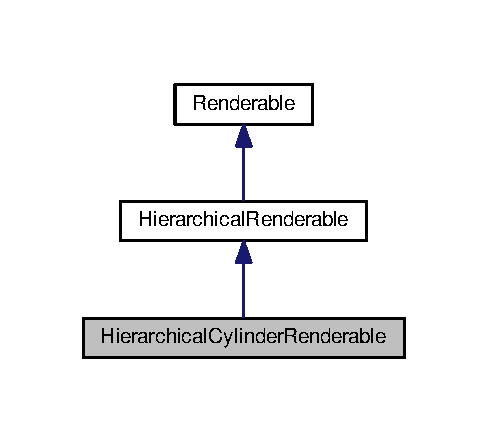
\includegraphics[width=234pt]{classHierarchicalCylinderRenderable__inherit__graph}
\end{center}
\end{figure}


Collaboration diagram for Hierarchical\+Cylinder\+Renderable\+:\nopagebreak
\begin{figure}[H]
\begin{center}
\leavevmode
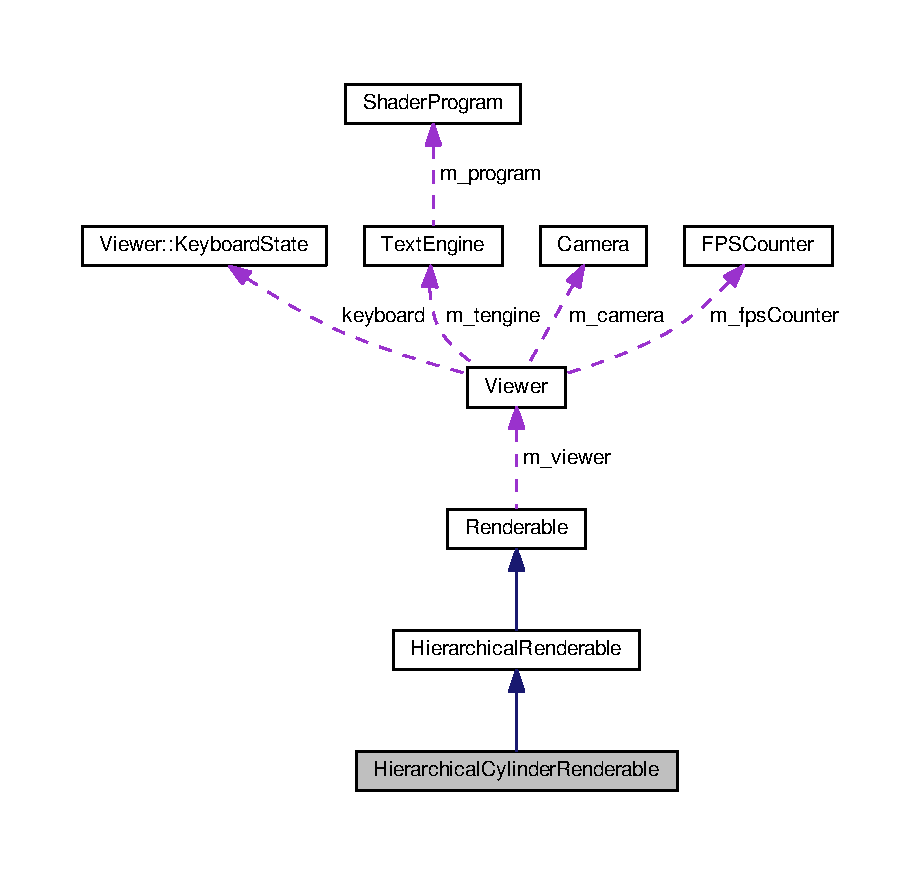
\includegraphics[width=350pt]{classHierarchicalCylinderRenderable__coll__graph}
\end{center}
\end{figure}
\subsection*{Public Member Functions}
\begin{DoxyCompactItemize}
\item 
\hyperlink{classHierarchicalCylinderRenderable_a35f2ede6a6f39ff9b770a06ee6dcb73c}{$\sim$\+Hierarchical\+Cylinder\+Renderable} ()
\item 
\hyperlink{classHierarchicalCylinderRenderable_a7c71cab100ac3d2a0d3e25591cc062f0}{Hierarchical\+Cylinder\+Renderable} (\hyperlink{ShaderProgram_8hpp_af8e4af1ad4c53875ee5d32ab7e1f4966}{Shader\+Program\+Ptr} program)
\end{DoxyCompactItemize}
\subsection*{Private Member Functions}
\begin{DoxyCompactItemize}
\item 
void \hyperlink{classHierarchicalCylinderRenderable_a4c2f4ead07f0c700e3b94f961a7be412}{do\+\_\+draw} ()
\begin{DoxyCompactList}\small\item\em Draw virtual function. \end{DoxyCompactList}\item 
void \hyperlink{classHierarchicalCylinderRenderable_a151ed55445a3bbbabdc9d19231a64a52}{do\+\_\+animate} (float time)
\begin{DoxyCompactList}\small\item\em Animate virtual function. \end{DoxyCompactList}\end{DoxyCompactItemize}
\subsection*{Private Attributes}
\begin{DoxyCompactItemize}
\item 
std\+::vector$<$ glm\+::vec3 $>$ \hyperlink{classHierarchicalCylinderRenderable_aa25417073ea90df6ea59d7d87050df49}{m\+\_\+positions}
\item 
std\+::vector$<$ glm\+::vec4 $>$ \hyperlink{classHierarchicalCylinderRenderable_aba8133be058d160bf53a66f205188e0a}{m\+\_\+colors}
\item 
std\+::vector$<$ glm\+::vec3 $>$ \hyperlink{classHierarchicalCylinderRenderable_af38a98b2fe2ca4b179d93b02dbf759fd}{m\+\_\+normals}
\item 
unsigned int \hyperlink{classHierarchicalCylinderRenderable_a7a69b3845a3dd2259b3c23a7c339232b}{m\+\_\+p\+Buffer}
\item 
unsigned int \hyperlink{classHierarchicalCylinderRenderable_a235710905d690d2ac3ee338ff486cf00}{m\+\_\+c\+Buffer}
\item 
unsigned int \hyperlink{classHierarchicalCylinderRenderable_aeede6a6e7c005db3949e90036855b0c5}{m\+\_\+n\+Buffer}
\end{DoxyCompactItemize}
\subsection*{Additional Inherited Members}


\subsection{Constructor \& Destructor Documentation}
\hypertarget{classHierarchicalCylinderRenderable_a35f2ede6a6f39ff9b770a06ee6dcb73c}{\index{Hierarchical\+Cylinder\+Renderable@{Hierarchical\+Cylinder\+Renderable}!````~Hierarchical\+Cylinder\+Renderable@{$\sim$\+Hierarchical\+Cylinder\+Renderable}}
\index{````~Hierarchical\+Cylinder\+Renderable@{$\sim$\+Hierarchical\+Cylinder\+Renderable}!Hierarchical\+Cylinder\+Renderable@{Hierarchical\+Cylinder\+Renderable}}
\subsubsection[{$\sim$\+Hierarchical\+Cylinder\+Renderable}]{\setlength{\rightskip}{0pt plus 5cm}Hierarchical\+Cylinder\+Renderable\+::$\sim$\+Hierarchical\+Cylinder\+Renderable (
\begin{DoxyParamCaption}
{}
\end{DoxyParamCaption}
)}}\label{classHierarchicalCylinderRenderable_a35f2ede6a6f39ff9b770a06ee6dcb73c}
\hypertarget{classHierarchicalCylinderRenderable_a7c71cab100ac3d2a0d3e25591cc062f0}{\index{Hierarchical\+Cylinder\+Renderable@{Hierarchical\+Cylinder\+Renderable}!Hierarchical\+Cylinder\+Renderable@{Hierarchical\+Cylinder\+Renderable}}
\index{Hierarchical\+Cylinder\+Renderable@{Hierarchical\+Cylinder\+Renderable}!Hierarchical\+Cylinder\+Renderable@{Hierarchical\+Cylinder\+Renderable}}
\subsubsection[{Hierarchical\+Cylinder\+Renderable}]{\setlength{\rightskip}{0pt plus 5cm}Hierarchical\+Cylinder\+Renderable\+::\+Hierarchical\+Cylinder\+Renderable (
\begin{DoxyParamCaption}
\item[{{\bf Shader\+Program\+Ptr}}]{program}
\end{DoxyParamCaption}
)}}\label{classHierarchicalCylinderRenderable_a7c71cab100ac3d2a0d3e25591cc062f0}


\subsection{Member Function Documentation}
\hypertarget{classHierarchicalCylinderRenderable_a151ed55445a3bbbabdc9d19231a64a52}{\index{Hierarchical\+Cylinder\+Renderable@{Hierarchical\+Cylinder\+Renderable}!do\+\_\+animate@{do\+\_\+animate}}
\index{do\+\_\+animate@{do\+\_\+animate}!Hierarchical\+Cylinder\+Renderable@{Hierarchical\+Cylinder\+Renderable}}
\subsubsection[{do\+\_\+animate}]{\setlength{\rightskip}{0pt plus 5cm}void Hierarchical\+Cylinder\+Renderable\+::do\+\_\+animate (
\begin{DoxyParamCaption}
\item[{float}]{time}
\end{DoxyParamCaption}
)\hspace{0.3cm}{\ttfamily [private]}, {\ttfamily [virtual]}}}\label{classHierarchicalCylinderRenderable_a151ed55445a3bbbabdc9d19231a64a52}
Implementation to animate this renderable. 
\begin{DoxyParams}{Parameters}
{\em time} & The current simulation time. \\
\hline
\end{DoxyParams}


Implements \hyperlink{classRenderable_aa5206322555c9dece40b21e797629b34}{Renderable}.

\hypertarget{classHierarchicalCylinderRenderable_a4c2f4ead07f0c700e3b94f961a7be412}{\index{Hierarchical\+Cylinder\+Renderable@{Hierarchical\+Cylinder\+Renderable}!do\+\_\+draw@{do\+\_\+draw}}
\index{do\+\_\+draw@{do\+\_\+draw}!Hierarchical\+Cylinder\+Renderable@{Hierarchical\+Cylinder\+Renderable}}
\subsubsection[{do\+\_\+draw}]{\setlength{\rightskip}{0pt plus 5cm}void Hierarchical\+Cylinder\+Renderable\+::do\+\_\+draw (
\begin{DoxyParamCaption}
{}
\end{DoxyParamCaption}
)\hspace{0.3cm}{\ttfamily [private]}, {\ttfamily [virtual]}}}\label{classHierarchicalCylinderRenderable_a4c2f4ead07f0c700e3b94f961a7be412}
Implementation to draw this renderable. 

Implements \hyperlink{classRenderable_a98ab6308c1d2b56dacda7c435fb38d5b}{Renderable}.



\subsection{Member Data Documentation}
\hypertarget{classHierarchicalCylinderRenderable_a235710905d690d2ac3ee338ff486cf00}{\index{Hierarchical\+Cylinder\+Renderable@{Hierarchical\+Cylinder\+Renderable}!m\+\_\+c\+Buffer@{m\+\_\+c\+Buffer}}
\index{m\+\_\+c\+Buffer@{m\+\_\+c\+Buffer}!Hierarchical\+Cylinder\+Renderable@{Hierarchical\+Cylinder\+Renderable}}
\subsubsection[{m\+\_\+c\+Buffer}]{\setlength{\rightskip}{0pt plus 5cm}unsigned int Hierarchical\+Cylinder\+Renderable\+::m\+\_\+c\+Buffer\hspace{0.3cm}{\ttfamily [private]}}}\label{classHierarchicalCylinderRenderable_a235710905d690d2ac3ee338ff486cf00}
\hypertarget{classHierarchicalCylinderRenderable_aba8133be058d160bf53a66f205188e0a}{\index{Hierarchical\+Cylinder\+Renderable@{Hierarchical\+Cylinder\+Renderable}!m\+\_\+colors@{m\+\_\+colors}}
\index{m\+\_\+colors@{m\+\_\+colors}!Hierarchical\+Cylinder\+Renderable@{Hierarchical\+Cylinder\+Renderable}}
\subsubsection[{m\+\_\+colors}]{\setlength{\rightskip}{0pt plus 5cm}std\+::vector$<$ glm\+::vec4 $>$ Hierarchical\+Cylinder\+Renderable\+::m\+\_\+colors\hspace{0.3cm}{\ttfamily [private]}}}\label{classHierarchicalCylinderRenderable_aba8133be058d160bf53a66f205188e0a}
\hypertarget{classHierarchicalCylinderRenderable_aeede6a6e7c005db3949e90036855b0c5}{\index{Hierarchical\+Cylinder\+Renderable@{Hierarchical\+Cylinder\+Renderable}!m\+\_\+n\+Buffer@{m\+\_\+n\+Buffer}}
\index{m\+\_\+n\+Buffer@{m\+\_\+n\+Buffer}!Hierarchical\+Cylinder\+Renderable@{Hierarchical\+Cylinder\+Renderable}}
\subsubsection[{m\+\_\+n\+Buffer}]{\setlength{\rightskip}{0pt plus 5cm}unsigned int Hierarchical\+Cylinder\+Renderable\+::m\+\_\+n\+Buffer\hspace{0.3cm}{\ttfamily [private]}}}\label{classHierarchicalCylinderRenderable_aeede6a6e7c005db3949e90036855b0c5}
\hypertarget{classHierarchicalCylinderRenderable_af38a98b2fe2ca4b179d93b02dbf759fd}{\index{Hierarchical\+Cylinder\+Renderable@{Hierarchical\+Cylinder\+Renderable}!m\+\_\+normals@{m\+\_\+normals}}
\index{m\+\_\+normals@{m\+\_\+normals}!Hierarchical\+Cylinder\+Renderable@{Hierarchical\+Cylinder\+Renderable}}
\subsubsection[{m\+\_\+normals}]{\setlength{\rightskip}{0pt plus 5cm}std\+::vector$<$ glm\+::vec3 $>$ Hierarchical\+Cylinder\+Renderable\+::m\+\_\+normals\hspace{0.3cm}{\ttfamily [private]}}}\label{classHierarchicalCylinderRenderable_af38a98b2fe2ca4b179d93b02dbf759fd}
\hypertarget{classHierarchicalCylinderRenderable_a7a69b3845a3dd2259b3c23a7c339232b}{\index{Hierarchical\+Cylinder\+Renderable@{Hierarchical\+Cylinder\+Renderable}!m\+\_\+p\+Buffer@{m\+\_\+p\+Buffer}}
\index{m\+\_\+p\+Buffer@{m\+\_\+p\+Buffer}!Hierarchical\+Cylinder\+Renderable@{Hierarchical\+Cylinder\+Renderable}}
\subsubsection[{m\+\_\+p\+Buffer}]{\setlength{\rightskip}{0pt plus 5cm}unsigned int Hierarchical\+Cylinder\+Renderable\+::m\+\_\+p\+Buffer\hspace{0.3cm}{\ttfamily [private]}}}\label{classHierarchicalCylinderRenderable_a7a69b3845a3dd2259b3c23a7c339232b}
\hypertarget{classHierarchicalCylinderRenderable_aa25417073ea90df6ea59d7d87050df49}{\index{Hierarchical\+Cylinder\+Renderable@{Hierarchical\+Cylinder\+Renderable}!m\+\_\+positions@{m\+\_\+positions}}
\index{m\+\_\+positions@{m\+\_\+positions}!Hierarchical\+Cylinder\+Renderable@{Hierarchical\+Cylinder\+Renderable}}
\subsubsection[{m\+\_\+positions}]{\setlength{\rightskip}{0pt plus 5cm}std\+::vector$<$ glm\+::vec3 $>$ Hierarchical\+Cylinder\+Renderable\+::m\+\_\+positions\hspace{0.3cm}{\ttfamily [private]}}}\label{classHierarchicalCylinderRenderable_aa25417073ea90df6ea59d7d87050df49}


The documentation for this class was generated from the following file\+:\begin{DoxyCompactItemize}
\item 
/home/chardon/\+Depot/ensimag/2\+A\+\_\+\+G3\+D/practicals/teacher\+Source/include/\hyperlink{HierarchicalCylinderRenderable_8hpp}{Hierarchical\+Cylinder\+Renderable.\+hpp}\end{DoxyCompactItemize}

\hypertarget{classHierarchicalMeshRenderable}{\section{Hierarchical\+Mesh\+Renderable Class Reference}
\label{classHierarchicalMeshRenderable}\index{Hierarchical\+Mesh\+Renderable@{Hierarchical\+Mesh\+Renderable}}
}


{\ttfamily \#include $<$Hierarchical\+Mesh\+Renderable.\+hpp$>$}



Inheritance diagram for Hierarchical\+Mesh\+Renderable\+:\nopagebreak
\begin{figure}[H]
\begin{center}
\leavevmode
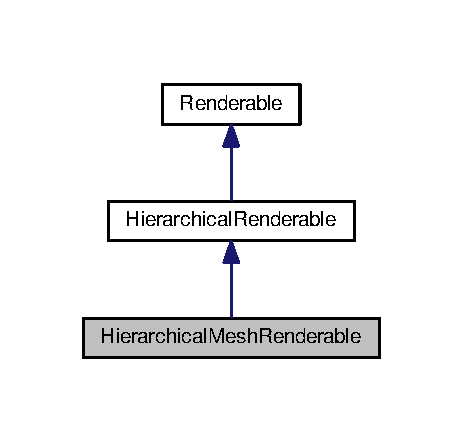
\includegraphics[width=222pt]{classHierarchicalMeshRenderable__inherit__graph}
\end{center}
\end{figure}


Collaboration diagram for Hierarchical\+Mesh\+Renderable\+:\nopagebreak
\begin{figure}[H]
\begin{center}
\leavevmode
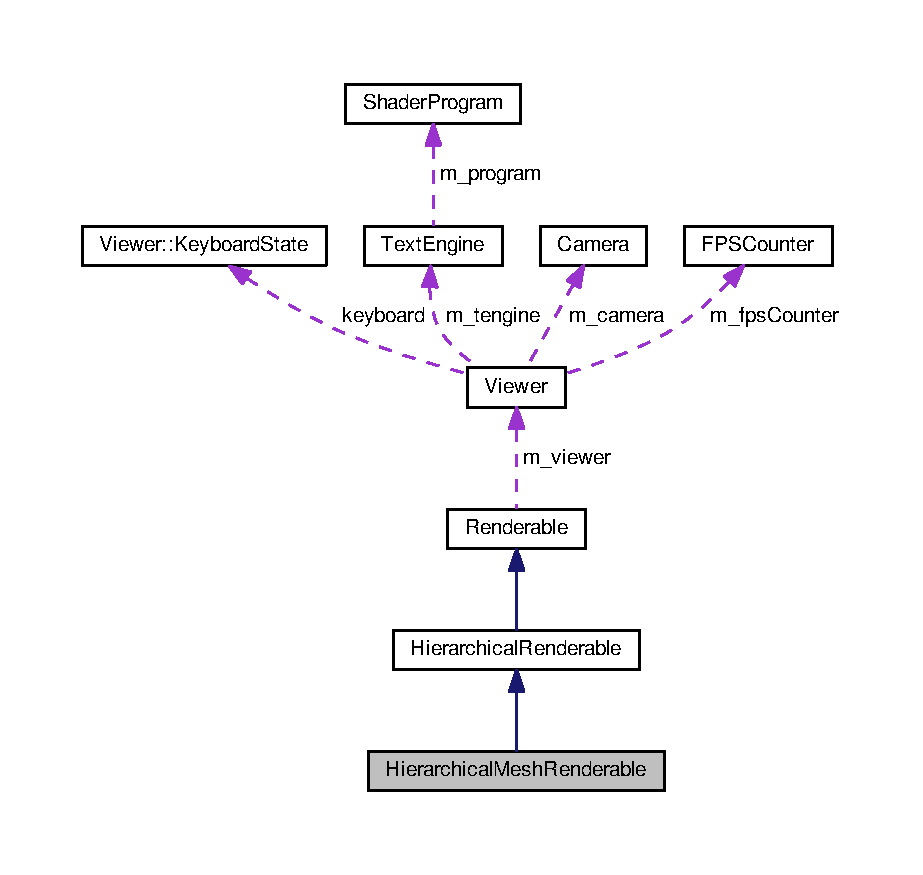
\includegraphics[width=350pt]{classHierarchicalMeshRenderable__coll__graph}
\end{center}
\end{figure}
\subsection*{Public Member Functions}
\begin{DoxyCompactItemize}
\item 
\hyperlink{classHierarchicalMeshRenderable_a7fdb59d99bca663e6e89c058a58a8ec7}{$\sim$\+Hierarchical\+Mesh\+Renderable} ()
\item 
\hyperlink{classHierarchicalMeshRenderable_addc544d58fd450811752f821ca2454cb}{Hierarchical\+Mesh\+Renderable} (\hyperlink{ShaderProgram_8hpp_af8e4af1ad4c53875ee5d32ab7e1f4966}{Shader\+Program\+Ptr} program, const std\+::string \&filename)
\end{DoxyCompactItemize}
\subsection*{Private Member Functions}
\begin{DoxyCompactItemize}
\item 
void \hyperlink{classHierarchicalMeshRenderable_a044c9f6688ee58184b8b3e4582f6baa1}{do\+\_\+draw} ()
\begin{DoxyCompactList}\small\item\em Draw virtual function. \end{DoxyCompactList}\item 
void \hyperlink{classHierarchicalMeshRenderable_a291689e73c0d7d2e733c587cd0062747}{do\+\_\+animate} (float time)
\begin{DoxyCompactList}\small\item\em Animate virtual function. \end{DoxyCompactList}\end{DoxyCompactItemize}
\subsection*{Private Attributes}
\begin{DoxyCompactItemize}
\item 
std\+::vector$<$ glm\+::vec3 $>$ \hyperlink{classHierarchicalMeshRenderable_a71289ce6648a162703a37814cb518459}{m\+\_\+positions}
\item 
std\+::vector$<$ glm\+::vec3 $>$ \hyperlink{classHierarchicalMeshRenderable_a0434afe3af71c5afcd7a3bc8318a0e98}{m\+\_\+normals}
\item 
std\+::vector$<$ glm\+::vec4 $>$ \hyperlink{classHierarchicalMeshRenderable_abcca72b5ae0157f6e9b23f3647939091}{m\+\_\+colors}
\item 
std\+::vector$<$ unsigned int $>$ \hyperlink{classHierarchicalMeshRenderable_a07550075b3137838436b798d2a772092}{m\+\_\+indices}
\item 
unsigned int \hyperlink{classHierarchicalMeshRenderable_abe9a8d6e06601db7f9e7ab8a5e306b78}{m\+\_\+p\+Buffer}
\item 
unsigned int \hyperlink{classHierarchicalMeshRenderable_a25985832ff7ad2ec41d818ba48190722}{m\+\_\+c\+Buffer}
\item 
unsigned int \hyperlink{classHierarchicalMeshRenderable_ae781c5aa305cc72608e3bd1b56129410}{m\+\_\+n\+Buffer}
\item 
unsigned int \hyperlink{classHierarchicalMeshRenderable_aaecf88387b5e1d8fe5c0d16bf5a7f6ab}{m\+\_\+i\+Buffer}
\end{DoxyCompactItemize}
\subsection*{Additional Inherited Members}


\subsection{Constructor \& Destructor Documentation}
\hypertarget{classHierarchicalMeshRenderable_a7fdb59d99bca663e6e89c058a58a8ec7}{\index{Hierarchical\+Mesh\+Renderable@{Hierarchical\+Mesh\+Renderable}!````~Hierarchical\+Mesh\+Renderable@{$\sim$\+Hierarchical\+Mesh\+Renderable}}
\index{````~Hierarchical\+Mesh\+Renderable@{$\sim$\+Hierarchical\+Mesh\+Renderable}!Hierarchical\+Mesh\+Renderable@{Hierarchical\+Mesh\+Renderable}}
\subsubsection[{$\sim$\+Hierarchical\+Mesh\+Renderable}]{\setlength{\rightskip}{0pt plus 5cm}Hierarchical\+Mesh\+Renderable\+::$\sim$\+Hierarchical\+Mesh\+Renderable (
\begin{DoxyParamCaption}
{}
\end{DoxyParamCaption}
)}}\label{classHierarchicalMeshRenderable_a7fdb59d99bca663e6e89c058a58a8ec7}
\hypertarget{classHierarchicalMeshRenderable_addc544d58fd450811752f821ca2454cb}{\index{Hierarchical\+Mesh\+Renderable@{Hierarchical\+Mesh\+Renderable}!Hierarchical\+Mesh\+Renderable@{Hierarchical\+Mesh\+Renderable}}
\index{Hierarchical\+Mesh\+Renderable@{Hierarchical\+Mesh\+Renderable}!Hierarchical\+Mesh\+Renderable@{Hierarchical\+Mesh\+Renderable}}
\subsubsection[{Hierarchical\+Mesh\+Renderable}]{\setlength{\rightskip}{0pt plus 5cm}Hierarchical\+Mesh\+Renderable\+::\+Hierarchical\+Mesh\+Renderable (
\begin{DoxyParamCaption}
\item[{{\bf Shader\+Program\+Ptr}}]{program, }
\item[{const std\+::string \&}]{filename}
\end{DoxyParamCaption}
)}}\label{classHierarchicalMeshRenderable_addc544d58fd450811752f821ca2454cb}


\subsection{Member Function Documentation}
\hypertarget{classHierarchicalMeshRenderable_a291689e73c0d7d2e733c587cd0062747}{\index{Hierarchical\+Mesh\+Renderable@{Hierarchical\+Mesh\+Renderable}!do\+\_\+animate@{do\+\_\+animate}}
\index{do\+\_\+animate@{do\+\_\+animate}!Hierarchical\+Mesh\+Renderable@{Hierarchical\+Mesh\+Renderable}}
\subsubsection[{do\+\_\+animate}]{\setlength{\rightskip}{0pt plus 5cm}void Hierarchical\+Mesh\+Renderable\+::do\+\_\+animate (
\begin{DoxyParamCaption}
\item[{float}]{time}
\end{DoxyParamCaption}
)\hspace{0.3cm}{\ttfamily [private]}, {\ttfamily [virtual]}}}\label{classHierarchicalMeshRenderable_a291689e73c0d7d2e733c587cd0062747}
Implementation to animate this renderable. 
\begin{DoxyParams}{Parameters}
{\em time} & The current simulation time. \\
\hline
\end{DoxyParams}


Implements \hyperlink{classRenderable_aa5206322555c9dece40b21e797629b34}{Renderable}.

\hypertarget{classHierarchicalMeshRenderable_a044c9f6688ee58184b8b3e4582f6baa1}{\index{Hierarchical\+Mesh\+Renderable@{Hierarchical\+Mesh\+Renderable}!do\+\_\+draw@{do\+\_\+draw}}
\index{do\+\_\+draw@{do\+\_\+draw}!Hierarchical\+Mesh\+Renderable@{Hierarchical\+Mesh\+Renderable}}
\subsubsection[{do\+\_\+draw}]{\setlength{\rightskip}{0pt plus 5cm}void Hierarchical\+Mesh\+Renderable\+::do\+\_\+draw (
\begin{DoxyParamCaption}
{}
\end{DoxyParamCaption}
)\hspace{0.3cm}{\ttfamily [private]}, {\ttfamily [virtual]}}}\label{classHierarchicalMeshRenderable_a044c9f6688ee58184b8b3e4582f6baa1}
Implementation to draw this renderable. 

Implements \hyperlink{classRenderable_a98ab6308c1d2b56dacda7c435fb38d5b}{Renderable}.



\subsection{Member Data Documentation}
\hypertarget{classHierarchicalMeshRenderable_a25985832ff7ad2ec41d818ba48190722}{\index{Hierarchical\+Mesh\+Renderable@{Hierarchical\+Mesh\+Renderable}!m\+\_\+c\+Buffer@{m\+\_\+c\+Buffer}}
\index{m\+\_\+c\+Buffer@{m\+\_\+c\+Buffer}!Hierarchical\+Mesh\+Renderable@{Hierarchical\+Mesh\+Renderable}}
\subsubsection[{m\+\_\+c\+Buffer}]{\setlength{\rightskip}{0pt plus 5cm}unsigned int Hierarchical\+Mesh\+Renderable\+::m\+\_\+c\+Buffer\hspace{0.3cm}{\ttfamily [private]}}}\label{classHierarchicalMeshRenderable_a25985832ff7ad2ec41d818ba48190722}
\hypertarget{classHierarchicalMeshRenderable_abcca72b5ae0157f6e9b23f3647939091}{\index{Hierarchical\+Mesh\+Renderable@{Hierarchical\+Mesh\+Renderable}!m\+\_\+colors@{m\+\_\+colors}}
\index{m\+\_\+colors@{m\+\_\+colors}!Hierarchical\+Mesh\+Renderable@{Hierarchical\+Mesh\+Renderable}}
\subsubsection[{m\+\_\+colors}]{\setlength{\rightskip}{0pt plus 5cm}std\+::vector$<$ glm\+::vec4 $>$ Hierarchical\+Mesh\+Renderable\+::m\+\_\+colors\hspace{0.3cm}{\ttfamily [private]}}}\label{classHierarchicalMeshRenderable_abcca72b5ae0157f6e9b23f3647939091}
\hypertarget{classHierarchicalMeshRenderable_aaecf88387b5e1d8fe5c0d16bf5a7f6ab}{\index{Hierarchical\+Mesh\+Renderable@{Hierarchical\+Mesh\+Renderable}!m\+\_\+i\+Buffer@{m\+\_\+i\+Buffer}}
\index{m\+\_\+i\+Buffer@{m\+\_\+i\+Buffer}!Hierarchical\+Mesh\+Renderable@{Hierarchical\+Mesh\+Renderable}}
\subsubsection[{m\+\_\+i\+Buffer}]{\setlength{\rightskip}{0pt plus 5cm}unsigned int Hierarchical\+Mesh\+Renderable\+::m\+\_\+i\+Buffer\hspace{0.3cm}{\ttfamily [private]}}}\label{classHierarchicalMeshRenderable_aaecf88387b5e1d8fe5c0d16bf5a7f6ab}
\hypertarget{classHierarchicalMeshRenderable_a07550075b3137838436b798d2a772092}{\index{Hierarchical\+Mesh\+Renderable@{Hierarchical\+Mesh\+Renderable}!m\+\_\+indices@{m\+\_\+indices}}
\index{m\+\_\+indices@{m\+\_\+indices}!Hierarchical\+Mesh\+Renderable@{Hierarchical\+Mesh\+Renderable}}
\subsubsection[{m\+\_\+indices}]{\setlength{\rightskip}{0pt plus 5cm}std\+::vector$<$ unsigned int $>$ Hierarchical\+Mesh\+Renderable\+::m\+\_\+indices\hspace{0.3cm}{\ttfamily [private]}}}\label{classHierarchicalMeshRenderable_a07550075b3137838436b798d2a772092}
\hypertarget{classHierarchicalMeshRenderable_ae781c5aa305cc72608e3bd1b56129410}{\index{Hierarchical\+Mesh\+Renderable@{Hierarchical\+Mesh\+Renderable}!m\+\_\+n\+Buffer@{m\+\_\+n\+Buffer}}
\index{m\+\_\+n\+Buffer@{m\+\_\+n\+Buffer}!Hierarchical\+Mesh\+Renderable@{Hierarchical\+Mesh\+Renderable}}
\subsubsection[{m\+\_\+n\+Buffer}]{\setlength{\rightskip}{0pt plus 5cm}unsigned int Hierarchical\+Mesh\+Renderable\+::m\+\_\+n\+Buffer\hspace{0.3cm}{\ttfamily [private]}}}\label{classHierarchicalMeshRenderable_ae781c5aa305cc72608e3bd1b56129410}
\hypertarget{classHierarchicalMeshRenderable_a0434afe3af71c5afcd7a3bc8318a0e98}{\index{Hierarchical\+Mesh\+Renderable@{Hierarchical\+Mesh\+Renderable}!m\+\_\+normals@{m\+\_\+normals}}
\index{m\+\_\+normals@{m\+\_\+normals}!Hierarchical\+Mesh\+Renderable@{Hierarchical\+Mesh\+Renderable}}
\subsubsection[{m\+\_\+normals}]{\setlength{\rightskip}{0pt plus 5cm}std\+::vector$<$ glm\+::vec3 $>$ Hierarchical\+Mesh\+Renderable\+::m\+\_\+normals\hspace{0.3cm}{\ttfamily [private]}}}\label{classHierarchicalMeshRenderable_a0434afe3af71c5afcd7a3bc8318a0e98}
\hypertarget{classHierarchicalMeshRenderable_abe9a8d6e06601db7f9e7ab8a5e306b78}{\index{Hierarchical\+Mesh\+Renderable@{Hierarchical\+Mesh\+Renderable}!m\+\_\+p\+Buffer@{m\+\_\+p\+Buffer}}
\index{m\+\_\+p\+Buffer@{m\+\_\+p\+Buffer}!Hierarchical\+Mesh\+Renderable@{Hierarchical\+Mesh\+Renderable}}
\subsubsection[{m\+\_\+p\+Buffer}]{\setlength{\rightskip}{0pt plus 5cm}unsigned int Hierarchical\+Mesh\+Renderable\+::m\+\_\+p\+Buffer\hspace{0.3cm}{\ttfamily [private]}}}\label{classHierarchicalMeshRenderable_abe9a8d6e06601db7f9e7ab8a5e306b78}
\hypertarget{classHierarchicalMeshRenderable_a71289ce6648a162703a37814cb518459}{\index{Hierarchical\+Mesh\+Renderable@{Hierarchical\+Mesh\+Renderable}!m\+\_\+positions@{m\+\_\+positions}}
\index{m\+\_\+positions@{m\+\_\+positions}!Hierarchical\+Mesh\+Renderable@{Hierarchical\+Mesh\+Renderable}}
\subsubsection[{m\+\_\+positions}]{\setlength{\rightskip}{0pt plus 5cm}std\+::vector$<$ glm\+::vec3 $>$ Hierarchical\+Mesh\+Renderable\+::m\+\_\+positions\hspace{0.3cm}{\ttfamily [private]}}}\label{classHierarchicalMeshRenderable_a71289ce6648a162703a37814cb518459}


The documentation for this class was generated from the following file\+:\begin{DoxyCompactItemize}
\item 
/home/chardon/\+Depot/ensimag/2\+A\+\_\+\+G3\+D/practicals/teacher\+Source/include/\hyperlink{HierarchicalMeshRenderable_8hpp}{Hierarchical\+Mesh\+Renderable.\+hpp}\end{DoxyCompactItemize}

\hypertarget{classHierarchicalRenderable}{\section{Hierarchical\+Renderable Class Reference}
\label{classHierarchicalRenderable}\index{Hierarchical\+Renderable@{Hierarchical\+Renderable}}
}


\hyperlink{classHierarchicalRenderable}{Hierarchical\+Renderable} interface.  




{\ttfamily \#include $<$Hierarchical\+Renderable.\+hpp$>$}



Inheritance diagram for Hierarchical\+Renderable\+:\nopagebreak
\begin{figure}[H]
\begin{center}
\leavevmode
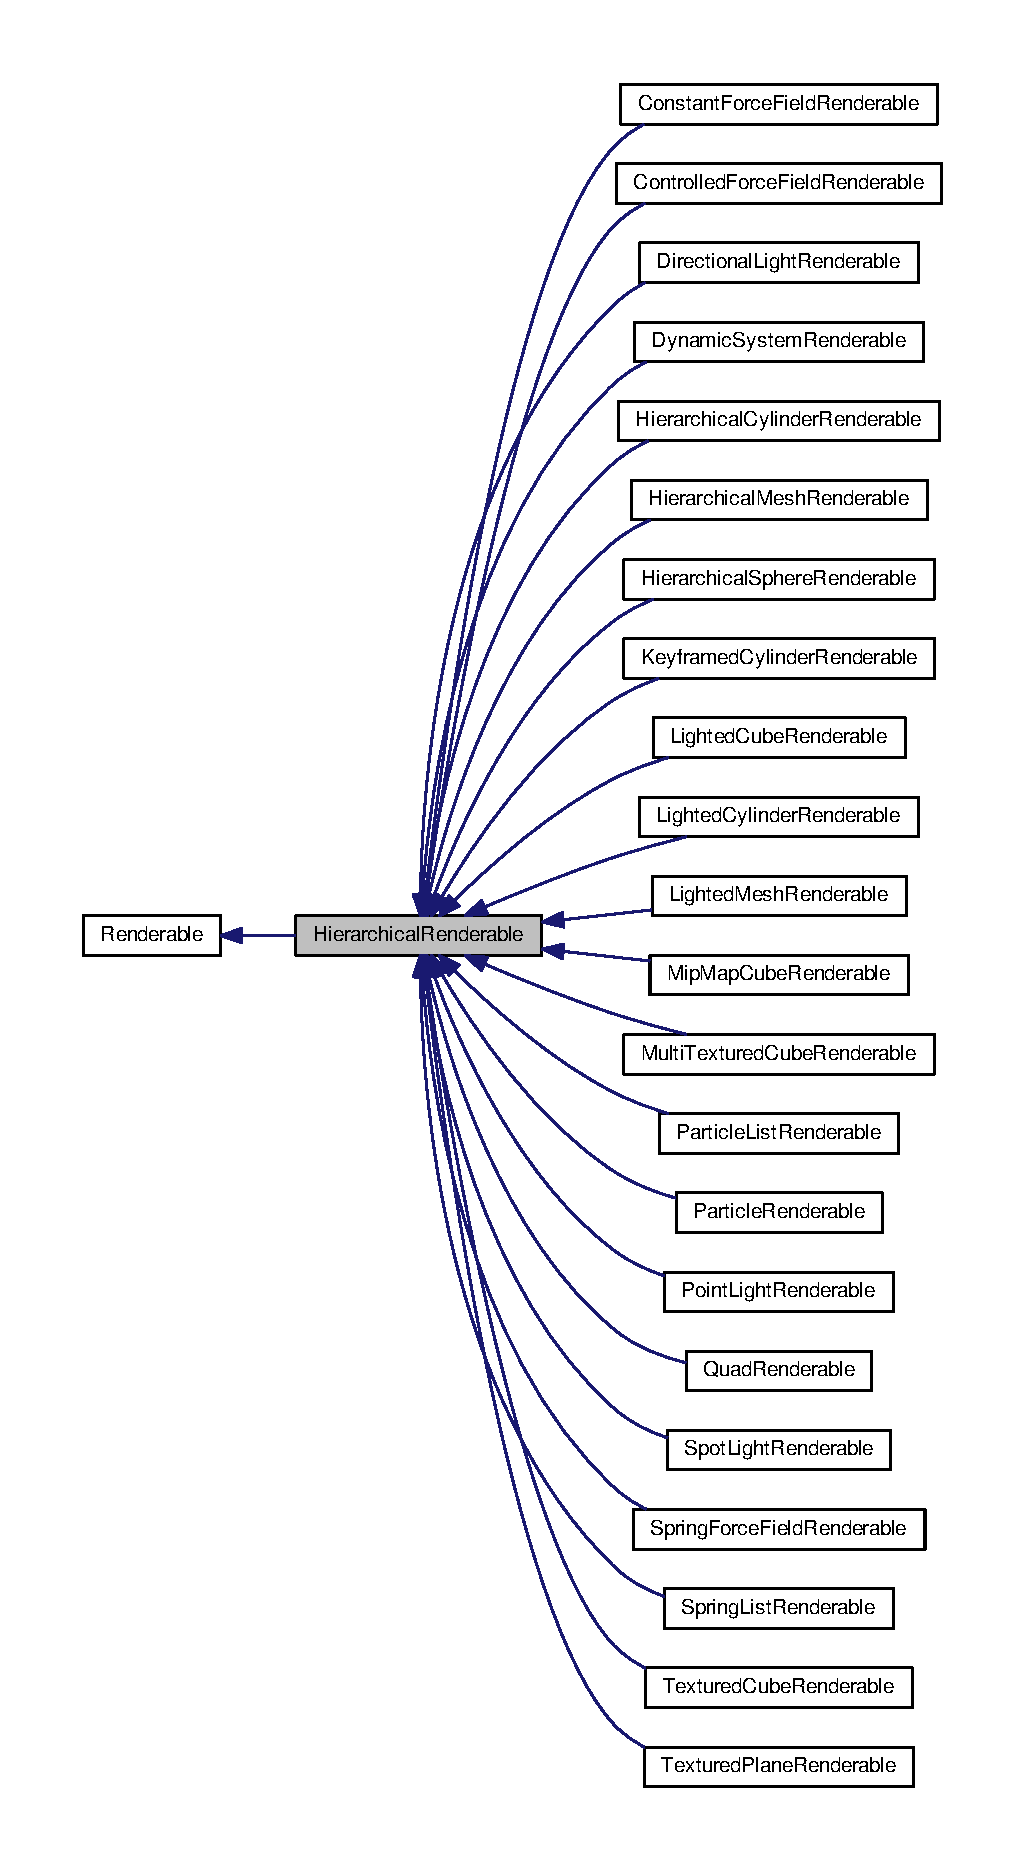
\includegraphics[height=550pt]{classHierarchicalRenderable__inherit__graph}
\end{center}
\end{figure}


Collaboration diagram for Hierarchical\+Renderable\+:\nopagebreak
\begin{figure}[H]
\begin{center}
\leavevmode
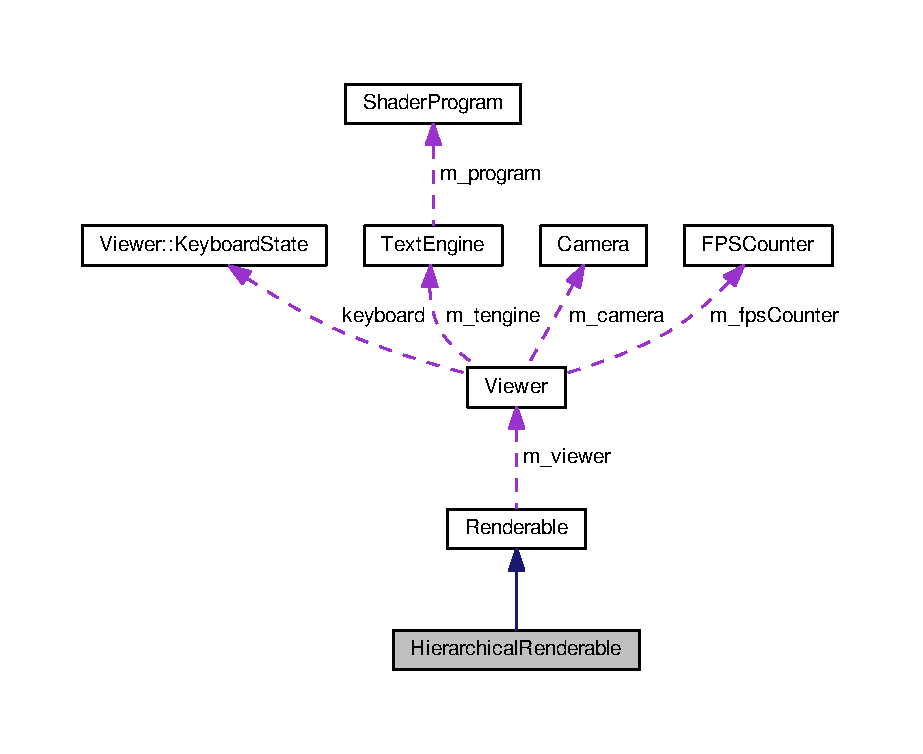
\includegraphics[width=350pt]{classHierarchicalRenderable__coll__graph}
\end{center}
\end{figure}
\subsection*{Public Member Functions}
\begin{DoxyCompactItemize}
\item 
virtual \hyperlink{classHierarchicalRenderable_a5b52660ebd8fc6ae221baf813359c5dc}{$\sim$\+Hierarchical\+Renderable} ()
\begin{DoxyCompactList}\small\item\em Instance destructor. \end{DoxyCompactList}\item 
\hyperlink{classHierarchicalRenderable_ad4869fc0d6af636308bef824d4882d66}{Hierarchical\+Renderable} (\hyperlink{ShaderProgram_8hpp_af8e4af1ad4c53875ee5d32ab7e1f4966}{Shader\+Program\+Ptr} shader\+Program)
\begin{DoxyCompactList}\small\item\em Instance constructor. \end{DoxyCompactList}\item 
void \hyperlink{classHierarchicalRenderable_a5f63685ed92393c8c43362540934b6c1}{update\+Model\+Matrix} ()
\begin{DoxyCompactList}\small\item\em Compute the model matrix of the instance. \end{DoxyCompactList}\item 
glm\+::mat4 \hyperlink{classHierarchicalRenderable_ac9ae8fd8114c2f8ce274b22661435d69}{compute\+Total\+Parent\+Transform} () const 
\begin{DoxyCompactList}\small\item\em Compute the total parent transformation. \end{DoxyCompactList}\item 
const glm\+::mat4 \& \hyperlink{classHierarchicalRenderable_ad2481b795d921e43d2697e36e5086727}{get\+Parent\+Transform} () const 
\begin{DoxyCompactList}\small\item\em Read only access to the parent transformation. \end{DoxyCompactList}\item 
void \hyperlink{classHierarchicalRenderable_aca80e8715bc7844967047602c5f9bb2d}{set\+Parent\+Transform} (const glm\+::mat4 \&parent\+Transform)
\begin{DoxyCompactList}\small\item\em Set the value of the parent transformation. \end{DoxyCompactList}\item 
const glm\+::mat4 \& \hyperlink{classHierarchicalRenderable_a201ce5c2ec7f323e6f3d0224a1eb31ef}{get\+Local\+Transform} () const 
\begin{DoxyCompactList}\small\item\em Read only access to the local transformation. \end{DoxyCompactList}\item 
void \hyperlink{classHierarchicalRenderable_a6dc43305b230675bd308566746aa1539}{set\+Local\+Transform} (const glm\+::mat4 \&local\+Transform)
\begin{DoxyCompactList}\small\item\em Set the value of the local transformation. \end{DoxyCompactList}\item 
std\+::vector\\*
$<$ \hyperlink{HierarchicalRenderable_8hpp_a9de1dda7f7ef0bca09b721bdb133964a}{Hierarchical\+Renderable\+Ptr} $>$ \& \hyperlink{classHierarchicalRenderable_a8a9b40b55e05760d76e39c8045bc9c71}{get\+Children} ()
\begin{DoxyCompactList}\small\item\em Access to the children of this renderable. \end{DoxyCompactList}\end{DoxyCompactItemize}
\subsection*{Static Public Member Functions}
\begin{DoxyCompactItemize}
\item 
static void \hyperlink{classHierarchicalRenderable_a0a8014f41a0439e86b18a78e8fbc448b}{add\+Child} (\hyperlink{HierarchicalRenderable_8hpp_a9de1dda7f7ef0bca09b721bdb133964a}{Hierarchical\+Renderable\+Ptr} parent, \hyperlink{HierarchicalRenderable_8hpp_a9de1dda7f7ef0bca09b721bdb133964a}{Hierarchical\+Renderable\+Ptr} child)
\begin{DoxyCompactList}\small\item\em Set hierarchical relationship between two \hyperlink{classHierarchicalRenderable}{Hierarchical\+Renderable} instances. \end{DoxyCompactList}\end{DoxyCompactItemize}
\subsection*{Private Member Functions}
\begin{DoxyCompactItemize}
\item 
virtual void \hyperlink{classHierarchicalRenderable_aedbaa13858872d5dcd7ce644da9a66e1}{before\+Draw} ()
\begin{DoxyCompactList}\small\item\em Perform computations before \hyperlink{classRenderable_a98ab6308c1d2b56dacda7c435fb38d5b}{do\+\_\+draw()} \end{DoxyCompactList}\item 
virtual void \hyperlink{classHierarchicalRenderable_a50fa8b46938a3da839829523838ddf2c}{after\+Draw} ()
\begin{DoxyCompactList}\small\item\em Perform computations after \hyperlink{classRenderable_a98ab6308c1d2b56dacda7c435fb38d5b}{do\+\_\+draw()} \end{DoxyCompactList}\item 
virtual void \hyperlink{classHierarchicalRenderable_a8de5020d6678c97050079150bcb131fa}{after\+Animate} (float time)
\begin{DoxyCompactList}\small\item\em Perform computations after \hyperlink{classRenderable_aa5206322555c9dece40b21e797629b34}{do\+\_\+animate()} \end{DoxyCompactList}\end{DoxyCompactItemize}
\subsection*{Private Attributes}
\begin{DoxyCompactItemize}
\item 
\hyperlink{HierarchicalRenderable_8hpp_a9de1dda7f7ef0bca09b721bdb133964a}{Hierarchical\+Renderable\+Ptr} \hyperlink{classHierarchicalRenderable_a8549e3830ff55e5f9ce5d6335421a207}{m\+\_\+parent}
\begin{DoxyCompactList}\small\item\em Pointer to the parent renderable. \end{DoxyCompactList}\item 
std\+::vector\\*
$<$ \hyperlink{HierarchicalRenderable_8hpp_a9de1dda7f7ef0bca09b721bdb133964a}{Hierarchical\+Renderable\+Ptr} $>$ \hyperlink{classHierarchicalRenderable_a0e3d2a642ba4d2ea58c595a1532a6c8a}{m\+\_\+children}
\begin{DoxyCompactList}\small\item\em List of the children of the instance. \end{DoxyCompactList}\item 
glm\+::mat4 \hyperlink{classHierarchicalRenderable_a03c1fee357c0148132468224d3480d92}{m\+\_\+parent\+Transform}
\begin{DoxyCompactList}\small\item\em Transformation with respect to the parent. \end{DoxyCompactList}\item 
glm\+::mat4 \hyperlink{classHierarchicalRenderable_a467e3ba997e6d98af60033fb74333c37}{m\+\_\+local\+Transform}
\begin{DoxyCompactList}\small\item\em Local transformation of this instance. \end{DoxyCompactList}\end{DoxyCompactItemize}
\subsection*{Additional Inherited Members}


\subsection{Detailed Description}
A hierarchical renderable is used to describe objects made of several renderables. The hierarchy is used to position objects relatively to others.

It becomes a powerful tool if the object is animated. In this case, animating a node of the hierarchy will implicitly animate its children.

The hierarchy is described by specifying the parent and the children of the instance. If the instance is the root of the hierarchy then it has no parent. If the instance is a leaf of the hierarchy then it has no children.

A \hyperlink{classHierarchicalRenderable}{Hierarchical\+Renderable} instance has two specific matrices\+:
\begin{DoxyItemize}
\item m\+\_\+parent\+Transform that defines the transformation with respect to the parent. The compositions of the parent transforms up to the root provides the local frame of the instance, in world space. The result of this composition is named the total parent transform.
\item m\+\_\+local\+Transform that defines an additional transformation, applied to the local frame of the instance, in order to obtain the model matrix. This transformation is not transmitted to the children of the instance. This allows to define a scale for example, without needing to apply the reverse operation to all its children.
\end{DoxyItemize}

Only the root instance is meant to be added to the \hyperlink{classViewer}{Viewer} instance\+: that root will take care itself to draw and animate all the hierarchy. However, if you want to interact with all the hierarchy, you will have to propagate yourself the interaction calls, such as \hyperlink{classRenderable_a49e39be950dca7a925b8b79c13241e6b}{do\+\_\+key\+Pressed\+Event()} to the children. This is not the default behavior as it could be easier to let the root the only instance that deals with interaction. 

\subsection{Constructor \& Destructor Documentation}
\hypertarget{classHierarchicalRenderable_a5b52660ebd8fc6ae221baf813359c5dc}{\index{Hierarchical\+Renderable@{Hierarchical\+Renderable}!````~Hierarchical\+Renderable@{$\sim$\+Hierarchical\+Renderable}}
\index{````~Hierarchical\+Renderable@{$\sim$\+Hierarchical\+Renderable}!Hierarchical\+Renderable@{Hierarchical\+Renderable}}
\subsubsection[{$\sim$\+Hierarchical\+Renderable}]{\setlength{\rightskip}{0pt plus 5cm}virtual Hierarchical\+Renderable\+::$\sim$\+Hierarchical\+Renderable (
\begin{DoxyParamCaption}
{}
\end{DoxyParamCaption}
)\hspace{0.3cm}{\ttfamily [virtual]}}}\label{classHierarchicalRenderable_a5b52660ebd8fc6ae221baf813359c5dc}
Since this class is meant to be derived (as it is abstract because we do not give an implementation for \hyperlink{classRenderable_a98ab6308c1d2b56dacda7c435fb38d5b}{Renderable\+::do\+\_\+draw()} for example), the destructor should be either public and virtual or protected and nonvirtual. We chose to make it public and virtual to let you delete concrete final class instances with a pointer to a Hierarchichal\+Renderable. \hypertarget{classHierarchicalRenderable_ad4869fc0d6af636308bef824d4882d66}{\index{Hierarchical\+Renderable@{Hierarchical\+Renderable}!Hierarchical\+Renderable@{Hierarchical\+Renderable}}
\index{Hierarchical\+Renderable@{Hierarchical\+Renderable}!Hierarchical\+Renderable@{Hierarchical\+Renderable}}
\subsubsection[{Hierarchical\+Renderable}]{\setlength{\rightskip}{0pt plus 5cm}Hierarchical\+Renderable\+::\+Hierarchical\+Renderable (
\begin{DoxyParamCaption}
\item[{{\bf Shader\+Program\+Ptr}}]{shader\+Program}
\end{DoxyParamCaption}
)}}\label{classHierarchicalRenderable_ad4869fc0d6af636308bef824d4882d66}
Initialize the local and parent transforms to identity, the model matrix to identity and the \hyperlink{classRenderable_ad4004cea2d9ca6cc91eb03b4ce885088}{m\+\_\+shader\+Program} to {\itshape shader\+Program}. 
\begin{DoxyParams}{Parameters}
{\em shader\+Program} & Shader program to use to draw this. \\
\hline
\end{DoxyParams}
\begin{DoxySeeAlso}{See also}
\hyperlink{classShaderProgram}{Shader\+Program} 
\end{DoxySeeAlso}


\subsection{Member Function Documentation}
\hypertarget{classHierarchicalRenderable_a0a8014f41a0439e86b18a78e8fbc448b}{\index{Hierarchical\+Renderable@{Hierarchical\+Renderable}!add\+Child@{add\+Child}}
\index{add\+Child@{add\+Child}!Hierarchical\+Renderable@{Hierarchical\+Renderable}}
\subsubsection[{add\+Child}]{\setlength{\rightskip}{0pt plus 5cm}static void Hierarchical\+Renderable\+::add\+Child (
\begin{DoxyParamCaption}
\item[{{\bf Hierarchical\+Renderable\+Ptr}}]{parent, }
\item[{{\bf Hierarchical\+Renderable\+Ptr}}]{child}
\end{DoxyParamCaption}
)\hspace{0.3cm}{\ttfamily [static]}}}\label{classHierarchicalRenderable_a0a8014f41a0439e86b18a78e8fbc448b}
This function adds {\itshape child} to the m\+\_\+children of {\itshape parent} and set the m\+\_\+parent member of {\itshape child} to {\itshape parent}.


\begin{DoxyParams}{Parameters}
{\em parent} & A pointer to the parent. \\
\hline
{\em child} & A pointer to the child.\\
\hline
\end{DoxyParams}
Note\+: the children and the parents of an instance are stored in a shared pointer. If we want to have a member function for this functionality, we would try to use \char`\"{}this\char`\"{}, either to add it to the children of an instance or to set it to be the parent of another instance. However, \char`\"{}this\char`\"{} is not a shared pointer, and if we try to create a shared pointer in the member function, that would mess completely with the memory management done in a shared pointer. \hypertarget{classHierarchicalRenderable_a8de5020d6678c97050079150bcb131fa}{\index{Hierarchical\+Renderable@{Hierarchical\+Renderable}!after\+Animate@{after\+Animate}}
\index{after\+Animate@{after\+Animate}!Hierarchical\+Renderable@{Hierarchical\+Renderable}}
\subsubsection[{after\+Animate}]{\setlength{\rightskip}{0pt plus 5cm}virtual void Hierarchical\+Renderable\+::after\+Animate (
\begin{DoxyParamCaption}
\item[{float}]{time}
\end{DoxyParamCaption}
)\hspace{0.3cm}{\ttfamily [private]}, {\ttfamily [virtual]}}}\label{classHierarchicalRenderable_a8de5020d6678c97050079150bcb131fa}


Reimplemented from \hyperlink{classRenderable_a027e4c23636f492df33461a23320a336}{Renderable}.

\hypertarget{classHierarchicalRenderable_a50fa8b46938a3da839829523838ddf2c}{\index{Hierarchical\+Renderable@{Hierarchical\+Renderable}!after\+Draw@{after\+Draw}}
\index{after\+Draw@{after\+Draw}!Hierarchical\+Renderable@{Hierarchical\+Renderable}}
\subsubsection[{after\+Draw}]{\setlength{\rightskip}{0pt plus 5cm}virtual void Hierarchical\+Renderable\+::after\+Draw (
\begin{DoxyParamCaption}
{}
\end{DoxyParamCaption}
)\hspace{0.3cm}{\ttfamily [private]}, {\ttfamily [virtual]}}}\label{classHierarchicalRenderable_a50fa8b46938a3da839829523838ddf2c}


Reimplemented from \hyperlink{classRenderable_a9c715cafdda260b94bf6fe12853a3bb7}{Renderable}.

\hypertarget{classHierarchicalRenderable_aedbaa13858872d5dcd7ce644da9a66e1}{\index{Hierarchical\+Renderable@{Hierarchical\+Renderable}!before\+Draw@{before\+Draw}}
\index{before\+Draw@{before\+Draw}!Hierarchical\+Renderable@{Hierarchical\+Renderable}}
\subsubsection[{before\+Draw}]{\setlength{\rightskip}{0pt plus 5cm}virtual void Hierarchical\+Renderable\+::before\+Draw (
\begin{DoxyParamCaption}
{}
\end{DoxyParamCaption}
)\hspace{0.3cm}{\ttfamily [private]}, {\ttfamily [virtual]}}}\label{classHierarchicalRenderable_aedbaa13858872d5dcd7ce644da9a66e1}


Reimplemented from \hyperlink{classRenderable_ad2fd96564194f598555b4f141e8c48be}{Renderable}.

\hypertarget{classHierarchicalRenderable_ac9ae8fd8114c2f8ce274b22661435d69}{\index{Hierarchical\+Renderable@{Hierarchical\+Renderable}!compute\+Total\+Parent\+Transform@{compute\+Total\+Parent\+Transform}}
\index{compute\+Total\+Parent\+Transform@{compute\+Total\+Parent\+Transform}!Hierarchical\+Renderable@{Hierarchical\+Renderable}}
\subsubsection[{compute\+Total\+Parent\+Transform}]{\setlength{\rightskip}{0pt plus 5cm}glm\+::mat4 Hierarchical\+Renderable\+::compute\+Total\+Parent\+Transform (
\begin{DoxyParamCaption}
{}
\end{DoxyParamCaption}
) const}}\label{classHierarchicalRenderable_ac9ae8fd8114c2f8ce274b22661435d69}
This function computes recursively the total parent transformation until it reaches the root of the hierarchy.

\begin{DoxyReturn}{Returns}
The total parent transformation matrix. 
\end{DoxyReturn}
\hypertarget{classHierarchicalRenderable_a8a9b40b55e05760d76e39c8045bc9c71}{\index{Hierarchical\+Renderable@{Hierarchical\+Renderable}!get\+Children@{get\+Children}}
\index{get\+Children@{get\+Children}!Hierarchical\+Renderable@{Hierarchical\+Renderable}}
\subsubsection[{get\+Children}]{\setlength{\rightskip}{0pt plus 5cm}std\+::vector$<$ {\bf Hierarchical\+Renderable\+Ptr} $>$\& Hierarchical\+Renderable\+::get\+Children (
\begin{DoxyParamCaption}
{}
\end{DoxyParamCaption}
)}}\label{classHierarchicalRenderable_a8a9b40b55e05760d76e39c8045bc9c71}
Get the children of this hierarchical renderable. \begin{DoxyReturn}{Returns}
A vector of hierarchical renderable shared pointers. 
\end{DoxyReturn}
\hypertarget{classHierarchicalRenderable_a201ce5c2ec7f323e6f3d0224a1eb31ef}{\index{Hierarchical\+Renderable@{Hierarchical\+Renderable}!get\+Local\+Transform@{get\+Local\+Transform}}
\index{get\+Local\+Transform@{get\+Local\+Transform}!Hierarchical\+Renderable@{Hierarchical\+Renderable}}
\subsubsection[{get\+Local\+Transform}]{\setlength{\rightskip}{0pt plus 5cm}const glm\+::mat4\& Hierarchical\+Renderable\+::get\+Local\+Transform (
\begin{DoxyParamCaption}
{}
\end{DoxyParamCaption}
) const}}\label{classHierarchicalRenderable_a201ce5c2ec7f323e6f3d0224a1eb31ef}
Write to the \hyperlink{classHierarchicalRenderable_a467e3ba997e6d98af60033fb74333c37}{m\+\_\+local\+Transform} matrix.

\begin{DoxyReturn}{Returns}
A read only reference to \hyperlink{classHierarchicalRenderable_a467e3ba997e6d98af60033fb74333c37}{m\+\_\+local\+Transform}, the local transformation matrix. 
\end{DoxyReturn}
\hypertarget{classHierarchicalRenderable_ad2481b795d921e43d2697e36e5086727}{\index{Hierarchical\+Renderable@{Hierarchical\+Renderable}!get\+Parent\+Transform@{get\+Parent\+Transform}}
\index{get\+Parent\+Transform@{get\+Parent\+Transform}!Hierarchical\+Renderable@{Hierarchical\+Renderable}}
\subsubsection[{get\+Parent\+Transform}]{\setlength{\rightskip}{0pt plus 5cm}const glm\+::mat4\& Hierarchical\+Renderable\+::get\+Parent\+Transform (
\begin{DoxyParamCaption}
{}
\end{DoxyParamCaption}
) const}}\label{classHierarchicalRenderable_ad2481b795d921e43d2697e36e5086727}
Allows to read the value of \hyperlink{classHierarchicalRenderable_a03c1fee357c0148132468224d3480d92}{m\+\_\+parent\+Transform}.

\begin{DoxyReturn}{Returns}
A read only reference to \hyperlink{classHierarchicalRenderable_a03c1fee357c0148132468224d3480d92}{m\+\_\+parent\+Transform}, the parent transformation matrix. 
\end{DoxyReturn}
\hypertarget{classHierarchicalRenderable_a6dc43305b230675bd308566746aa1539}{\index{Hierarchical\+Renderable@{Hierarchical\+Renderable}!set\+Local\+Transform@{set\+Local\+Transform}}
\index{set\+Local\+Transform@{set\+Local\+Transform}!Hierarchical\+Renderable@{Hierarchical\+Renderable}}
\subsubsection[{set\+Local\+Transform}]{\setlength{\rightskip}{0pt plus 5cm}void Hierarchical\+Renderable\+::set\+Local\+Transform (
\begin{DoxyParamCaption}
\item[{const glm\+::mat4 \&}]{local\+Transform}
\end{DoxyParamCaption}
)}}\label{classHierarchicalRenderable_a6dc43305b230675bd308566746aa1539}
Write to the \hyperlink{classHierarchicalRenderable_a467e3ba997e6d98af60033fb74333c37}{m\+\_\+local\+Transform} matrix.


\begin{DoxyParams}{Parameters}
{\em local\+Transform} & The new local transformation matrix. \\
\hline
\end{DoxyParams}
\hypertarget{classHierarchicalRenderable_aca80e8715bc7844967047602c5f9bb2d}{\index{Hierarchical\+Renderable@{Hierarchical\+Renderable}!set\+Parent\+Transform@{set\+Parent\+Transform}}
\index{set\+Parent\+Transform@{set\+Parent\+Transform}!Hierarchical\+Renderable@{Hierarchical\+Renderable}}
\subsubsection[{set\+Parent\+Transform}]{\setlength{\rightskip}{0pt plus 5cm}void Hierarchical\+Renderable\+::set\+Parent\+Transform (
\begin{DoxyParamCaption}
\item[{const glm\+::mat4 \&}]{parent\+Transform}
\end{DoxyParamCaption}
)}}\label{classHierarchicalRenderable_aca80e8715bc7844967047602c5f9bb2d}
Write to the \hyperlink{classHierarchicalRenderable_a03c1fee357c0148132468224d3480d92}{m\+\_\+parent\+Transform} matrix. Avoid to have non uniform scale here\+: prefer to make it in the local transform. Otherwise, you will obtain shearing.


\begin{DoxyParams}{Parameters}
{\em parent\+Transform} & The new parent transformation matrix. \\
\hline
\end{DoxyParams}
\hypertarget{classHierarchicalRenderable_a5f63685ed92393c8c43362540934b6c1}{\index{Hierarchical\+Renderable@{Hierarchical\+Renderable}!update\+Model\+Matrix@{update\+Model\+Matrix}}
\index{update\+Model\+Matrix@{update\+Model\+Matrix}!Hierarchical\+Renderable@{Hierarchical\+Renderable}}
\subsubsection[{update\+Model\+Matrix}]{\setlength{\rightskip}{0pt plus 5cm}void Hierarchical\+Renderable\+::update\+Model\+Matrix (
\begin{DoxyParamCaption}
{}
\end{DoxyParamCaption}
)}}\label{classHierarchicalRenderable_a5f63685ed92393c8c43362540934b6c1}
Since a model matrix is the transformation from the object coordinates to the world coordinates, it should be computed thanks to the hierarchy and the matrices \hyperlink{classHierarchicalRenderable_a03c1fee357c0148132468224d3480d92}{m\+\_\+parent\+Transform}. This computation is done in this function and should be typically applied before drawing a hierarchical renderable. The result is stored in \hyperlink{classRenderable_ab3a7f6112bd9d8c37ab10dac24186b25}{m\+\_\+model}. 

\subsection{Member Data Documentation}
\hypertarget{classHierarchicalRenderable_a0e3d2a642ba4d2ea58c595a1532a6c8a}{\index{Hierarchical\+Renderable@{Hierarchical\+Renderable}!m\+\_\+children@{m\+\_\+children}}
\index{m\+\_\+children@{m\+\_\+children}!Hierarchical\+Renderable@{Hierarchical\+Renderable}}
\subsubsection[{m\+\_\+children}]{\setlength{\rightskip}{0pt plus 5cm}std\+::vector$<$ {\bf Hierarchical\+Renderable\+Ptr} $>$ Hierarchical\+Renderable\+::m\+\_\+children\hspace{0.3cm}{\ttfamily [private]}}}\label{classHierarchicalRenderable_a0e3d2a642ba4d2ea58c595a1532a6c8a}
This list contains all the children of the instance. Those children all have this as a parent. \hypertarget{classHierarchicalRenderable_a467e3ba997e6d98af60033fb74333c37}{\index{Hierarchical\+Renderable@{Hierarchical\+Renderable}!m\+\_\+local\+Transform@{m\+\_\+local\+Transform}}
\index{m\+\_\+local\+Transform@{m\+\_\+local\+Transform}!Hierarchical\+Renderable@{Hierarchical\+Renderable}}
\subsubsection[{m\+\_\+local\+Transform}]{\setlength{\rightskip}{0pt plus 5cm}glm\+::mat4 Hierarchical\+Renderable\+::m\+\_\+local\+Transform\hspace{0.3cm}{\ttfamily [private]}}}\label{classHierarchicalRenderable_a467e3ba997e6d98af60033fb74333c37}
This transformation is applied to the global parent transformation to give the model matrix. It is particularly useful to deform the geometry of the object using scaling. Keep in mind that this transformation will N\+O\+T be used by the children. \hypertarget{classHierarchicalRenderable_a8549e3830ff55e5f9ce5d6335421a207}{\index{Hierarchical\+Renderable@{Hierarchical\+Renderable}!m\+\_\+parent@{m\+\_\+parent}}
\index{m\+\_\+parent@{m\+\_\+parent}!Hierarchical\+Renderable@{Hierarchical\+Renderable}}
\subsubsection[{m\+\_\+parent}]{\setlength{\rightskip}{0pt plus 5cm}{\bf Hierarchical\+Renderable\+Ptr} Hierarchical\+Renderable\+::m\+\_\+parent\hspace{0.3cm}{\ttfamily [private]}}}\label{classHierarchicalRenderable_a8549e3830ff55e5f9ce5d6335421a207}
If it has no parent then the pointer value is nullptr. This is the case if the instance is the root of the hierarchy.

The instance is positioned relatively to the parent. \hypertarget{classHierarchicalRenderable_a03c1fee357c0148132468224d3480d92}{\index{Hierarchical\+Renderable@{Hierarchical\+Renderable}!m\+\_\+parent\+Transform@{m\+\_\+parent\+Transform}}
\index{m\+\_\+parent\+Transform@{m\+\_\+parent\+Transform}!Hierarchical\+Renderable@{Hierarchical\+Renderable}}
\subsubsection[{m\+\_\+parent\+Transform}]{\setlength{\rightskip}{0pt plus 5cm}glm\+::mat4 Hierarchical\+Renderable\+::m\+\_\+parent\+Transform\hspace{0.3cm}{\ttfamily [private]}}}\label{classHierarchicalRenderable_a03c1fee357c0148132468224d3480d92}
This matrix gives the transformation of this instance relatively to its parent. If it has no parent the the matrix is set to identity. Keep in mind that this transformation will be used by the children. 

The documentation for this class was generated from the following file\+:\begin{DoxyCompactItemize}
\item 
/home/chardon/\+Depot/ensimag/2\+A\+\_\+\+G3\+D/practicals/teacher\+Source/include/\hyperlink{HierarchicalRenderable_8hpp}{Hierarchical\+Renderable.\+hpp}\end{DoxyCompactItemize}

\hypertarget{classHierarchicalSphereRenderable}{\section{Hierarchical\+Sphere\+Renderable Class Reference}
\label{classHierarchicalSphereRenderable}\index{Hierarchical\+Sphere\+Renderable@{Hierarchical\+Sphere\+Renderable}}
}


{\ttfamily \#include $<$Hierarchical\+Sphere\+Renderable.\+hpp$>$}



Inheritance diagram for Hierarchical\+Sphere\+Renderable\+:\nopagebreak
\begin{figure}[H]
\begin{center}
\leavevmode
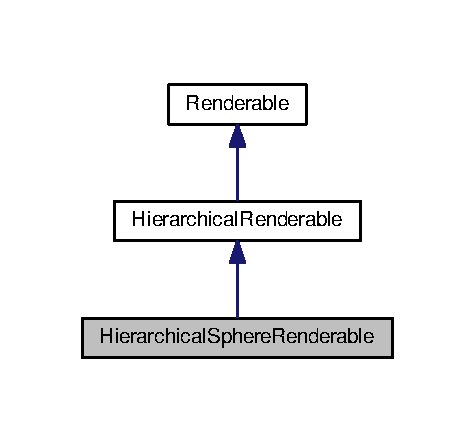
\includegraphics[width=228pt]{classHierarchicalSphereRenderable__inherit__graph}
\end{center}
\end{figure}


Collaboration diagram for Hierarchical\+Sphere\+Renderable\+:\nopagebreak
\begin{figure}[H]
\begin{center}
\leavevmode
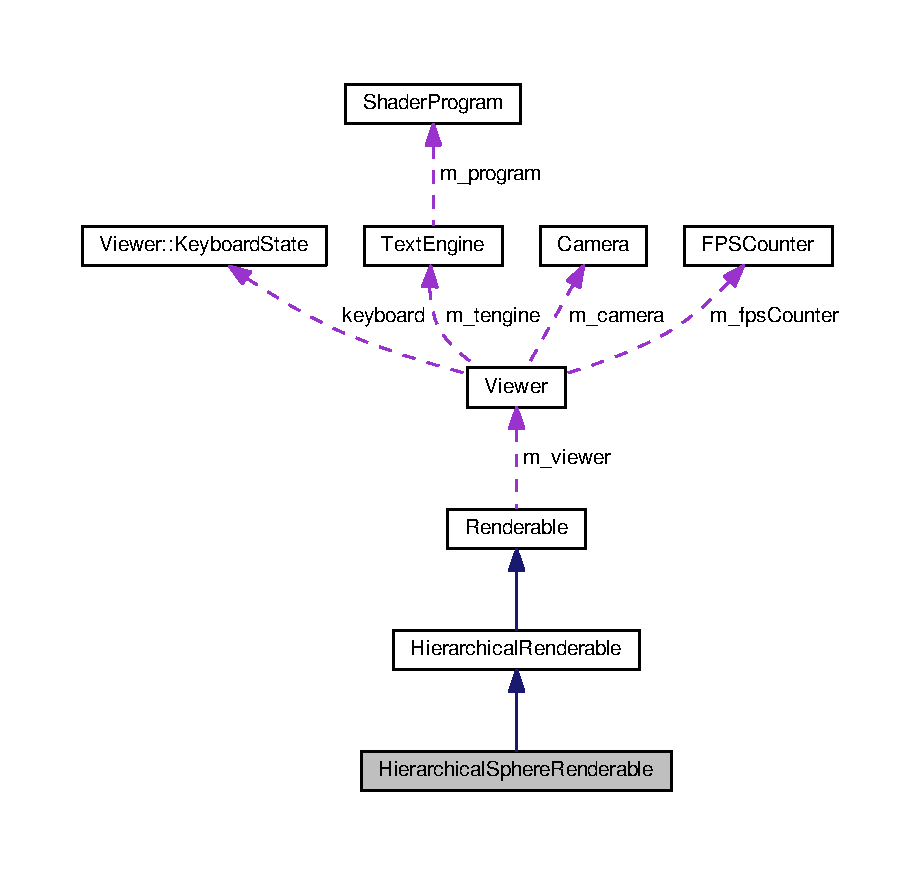
\includegraphics[width=350pt]{classHierarchicalSphereRenderable__coll__graph}
\end{center}
\end{figure}
\subsection*{Public Member Functions}
\begin{DoxyCompactItemize}
\item 
\hyperlink{classHierarchicalSphereRenderable_ab11112da0ea3de1003b8b5b6f910e555}{$\sim$\+Hierarchical\+Sphere\+Renderable} ()
\item 
\hyperlink{classHierarchicalSphereRenderable_a710cadb8babef39601f98a83ad54dab4}{Hierarchical\+Sphere\+Renderable} (\hyperlink{ShaderProgram_8hpp_af8e4af1ad4c53875ee5d32ab7e1f4966}{Shader\+Program\+Ptr} program)
\end{DoxyCompactItemize}
\subsection*{Private Member Functions}
\begin{DoxyCompactItemize}
\item 
void \hyperlink{classHierarchicalSphereRenderable_a5216d2b3a015c11f888e6ac268362926}{do\+\_\+draw} ()
\begin{DoxyCompactList}\small\item\em Draw virtual function. \end{DoxyCompactList}\item 
void \hyperlink{classHierarchicalSphereRenderable_a712e4865f38fced13bc3aa5be7a17764}{do\+\_\+animate} (float time)
\begin{DoxyCompactList}\small\item\em Animate virtual function. \end{DoxyCompactList}\end{DoxyCompactItemize}
\subsection*{Private Attributes}
\begin{DoxyCompactItemize}
\item 
std\+::vector$<$ glm\+::vec3 $>$ \hyperlink{classHierarchicalSphereRenderable_a78da197355ab6d1e30978f0a9b24f8d1}{m\+\_\+positions}
\item 
std\+::vector$<$ glm\+::vec4 $>$ \hyperlink{classHierarchicalSphereRenderable_a8875eaeab3e4381ab00de2cfb8f650ba}{m\+\_\+colors}
\item 
std\+::vector$<$ glm\+::vec3 $>$ \hyperlink{classHierarchicalSphereRenderable_a61da071fdee1bd9c74f4a56e8264b90c}{m\+\_\+normals}
\item 
unsigned int \hyperlink{classHierarchicalSphereRenderable_a10b5df7bebe5790780d7f12dac654f5f}{m\+\_\+p\+Buffer}
\item 
unsigned int \hyperlink{classHierarchicalSphereRenderable_ae563ee9c7597aeaf5c00cc430626bdf6}{m\+\_\+c\+Buffer}
\item 
unsigned int \hyperlink{classHierarchicalSphereRenderable_a3d0052db7a742c21b4b88933ba073fb3}{m\+\_\+n\+Buffer}
\end{DoxyCompactItemize}
\subsection*{Additional Inherited Members}


\subsection{Constructor \& Destructor Documentation}
\hypertarget{classHierarchicalSphereRenderable_ab11112da0ea3de1003b8b5b6f910e555}{\index{Hierarchical\+Sphere\+Renderable@{Hierarchical\+Sphere\+Renderable}!````~Hierarchical\+Sphere\+Renderable@{$\sim$\+Hierarchical\+Sphere\+Renderable}}
\index{````~Hierarchical\+Sphere\+Renderable@{$\sim$\+Hierarchical\+Sphere\+Renderable}!Hierarchical\+Sphere\+Renderable@{Hierarchical\+Sphere\+Renderable}}
\subsubsection[{$\sim$\+Hierarchical\+Sphere\+Renderable}]{\setlength{\rightskip}{0pt plus 5cm}Hierarchical\+Sphere\+Renderable\+::$\sim$\+Hierarchical\+Sphere\+Renderable (
\begin{DoxyParamCaption}
{}
\end{DoxyParamCaption}
)}}\label{classHierarchicalSphereRenderable_ab11112da0ea3de1003b8b5b6f910e555}
\hypertarget{classHierarchicalSphereRenderable_a710cadb8babef39601f98a83ad54dab4}{\index{Hierarchical\+Sphere\+Renderable@{Hierarchical\+Sphere\+Renderable}!Hierarchical\+Sphere\+Renderable@{Hierarchical\+Sphere\+Renderable}}
\index{Hierarchical\+Sphere\+Renderable@{Hierarchical\+Sphere\+Renderable}!Hierarchical\+Sphere\+Renderable@{Hierarchical\+Sphere\+Renderable}}
\subsubsection[{Hierarchical\+Sphere\+Renderable}]{\setlength{\rightskip}{0pt plus 5cm}Hierarchical\+Sphere\+Renderable\+::\+Hierarchical\+Sphere\+Renderable (
\begin{DoxyParamCaption}
\item[{{\bf Shader\+Program\+Ptr}}]{program}
\end{DoxyParamCaption}
)}}\label{classHierarchicalSphereRenderable_a710cadb8babef39601f98a83ad54dab4}


\subsection{Member Function Documentation}
\hypertarget{classHierarchicalSphereRenderable_a712e4865f38fced13bc3aa5be7a17764}{\index{Hierarchical\+Sphere\+Renderable@{Hierarchical\+Sphere\+Renderable}!do\+\_\+animate@{do\+\_\+animate}}
\index{do\+\_\+animate@{do\+\_\+animate}!Hierarchical\+Sphere\+Renderable@{Hierarchical\+Sphere\+Renderable}}
\subsubsection[{do\+\_\+animate}]{\setlength{\rightskip}{0pt plus 5cm}void Hierarchical\+Sphere\+Renderable\+::do\+\_\+animate (
\begin{DoxyParamCaption}
\item[{float}]{time}
\end{DoxyParamCaption}
)\hspace{0.3cm}{\ttfamily [private]}, {\ttfamily [virtual]}}}\label{classHierarchicalSphereRenderable_a712e4865f38fced13bc3aa5be7a17764}
Implementation to animate this renderable. 
\begin{DoxyParams}{Parameters}
{\em time} & The current simulation time. \\
\hline
\end{DoxyParams}


Implements \hyperlink{classRenderable_aa5206322555c9dece40b21e797629b34}{Renderable}.

\hypertarget{classHierarchicalSphereRenderable_a5216d2b3a015c11f888e6ac268362926}{\index{Hierarchical\+Sphere\+Renderable@{Hierarchical\+Sphere\+Renderable}!do\+\_\+draw@{do\+\_\+draw}}
\index{do\+\_\+draw@{do\+\_\+draw}!Hierarchical\+Sphere\+Renderable@{Hierarchical\+Sphere\+Renderable}}
\subsubsection[{do\+\_\+draw}]{\setlength{\rightskip}{0pt plus 5cm}void Hierarchical\+Sphere\+Renderable\+::do\+\_\+draw (
\begin{DoxyParamCaption}
{}
\end{DoxyParamCaption}
)\hspace{0.3cm}{\ttfamily [private]}, {\ttfamily [virtual]}}}\label{classHierarchicalSphereRenderable_a5216d2b3a015c11f888e6ac268362926}
Implementation to draw this renderable. 

Implements \hyperlink{classRenderable_a98ab6308c1d2b56dacda7c435fb38d5b}{Renderable}.



\subsection{Member Data Documentation}
\hypertarget{classHierarchicalSphereRenderable_ae563ee9c7597aeaf5c00cc430626bdf6}{\index{Hierarchical\+Sphere\+Renderable@{Hierarchical\+Sphere\+Renderable}!m\+\_\+c\+Buffer@{m\+\_\+c\+Buffer}}
\index{m\+\_\+c\+Buffer@{m\+\_\+c\+Buffer}!Hierarchical\+Sphere\+Renderable@{Hierarchical\+Sphere\+Renderable}}
\subsubsection[{m\+\_\+c\+Buffer}]{\setlength{\rightskip}{0pt plus 5cm}unsigned int Hierarchical\+Sphere\+Renderable\+::m\+\_\+c\+Buffer\hspace{0.3cm}{\ttfamily [private]}}}\label{classHierarchicalSphereRenderable_ae563ee9c7597aeaf5c00cc430626bdf6}
\hypertarget{classHierarchicalSphereRenderable_a8875eaeab3e4381ab00de2cfb8f650ba}{\index{Hierarchical\+Sphere\+Renderable@{Hierarchical\+Sphere\+Renderable}!m\+\_\+colors@{m\+\_\+colors}}
\index{m\+\_\+colors@{m\+\_\+colors}!Hierarchical\+Sphere\+Renderable@{Hierarchical\+Sphere\+Renderable}}
\subsubsection[{m\+\_\+colors}]{\setlength{\rightskip}{0pt plus 5cm}std\+::vector$<$ glm\+::vec4 $>$ Hierarchical\+Sphere\+Renderable\+::m\+\_\+colors\hspace{0.3cm}{\ttfamily [private]}}}\label{classHierarchicalSphereRenderable_a8875eaeab3e4381ab00de2cfb8f650ba}
\hypertarget{classHierarchicalSphereRenderable_a3d0052db7a742c21b4b88933ba073fb3}{\index{Hierarchical\+Sphere\+Renderable@{Hierarchical\+Sphere\+Renderable}!m\+\_\+n\+Buffer@{m\+\_\+n\+Buffer}}
\index{m\+\_\+n\+Buffer@{m\+\_\+n\+Buffer}!Hierarchical\+Sphere\+Renderable@{Hierarchical\+Sphere\+Renderable}}
\subsubsection[{m\+\_\+n\+Buffer}]{\setlength{\rightskip}{0pt plus 5cm}unsigned int Hierarchical\+Sphere\+Renderable\+::m\+\_\+n\+Buffer\hspace{0.3cm}{\ttfamily [private]}}}\label{classHierarchicalSphereRenderable_a3d0052db7a742c21b4b88933ba073fb3}
\hypertarget{classHierarchicalSphereRenderable_a61da071fdee1bd9c74f4a56e8264b90c}{\index{Hierarchical\+Sphere\+Renderable@{Hierarchical\+Sphere\+Renderable}!m\+\_\+normals@{m\+\_\+normals}}
\index{m\+\_\+normals@{m\+\_\+normals}!Hierarchical\+Sphere\+Renderable@{Hierarchical\+Sphere\+Renderable}}
\subsubsection[{m\+\_\+normals}]{\setlength{\rightskip}{0pt plus 5cm}std\+::vector$<$ glm\+::vec3 $>$ Hierarchical\+Sphere\+Renderable\+::m\+\_\+normals\hspace{0.3cm}{\ttfamily [private]}}}\label{classHierarchicalSphereRenderable_a61da071fdee1bd9c74f4a56e8264b90c}
\hypertarget{classHierarchicalSphereRenderable_a10b5df7bebe5790780d7f12dac654f5f}{\index{Hierarchical\+Sphere\+Renderable@{Hierarchical\+Sphere\+Renderable}!m\+\_\+p\+Buffer@{m\+\_\+p\+Buffer}}
\index{m\+\_\+p\+Buffer@{m\+\_\+p\+Buffer}!Hierarchical\+Sphere\+Renderable@{Hierarchical\+Sphere\+Renderable}}
\subsubsection[{m\+\_\+p\+Buffer}]{\setlength{\rightskip}{0pt plus 5cm}unsigned int Hierarchical\+Sphere\+Renderable\+::m\+\_\+p\+Buffer\hspace{0.3cm}{\ttfamily [private]}}}\label{classHierarchicalSphereRenderable_a10b5df7bebe5790780d7f12dac654f5f}
\hypertarget{classHierarchicalSphereRenderable_a78da197355ab6d1e30978f0a9b24f8d1}{\index{Hierarchical\+Sphere\+Renderable@{Hierarchical\+Sphere\+Renderable}!m\+\_\+positions@{m\+\_\+positions}}
\index{m\+\_\+positions@{m\+\_\+positions}!Hierarchical\+Sphere\+Renderable@{Hierarchical\+Sphere\+Renderable}}
\subsubsection[{m\+\_\+positions}]{\setlength{\rightskip}{0pt plus 5cm}std\+::vector$<$ glm\+::vec3 $>$ Hierarchical\+Sphere\+Renderable\+::m\+\_\+positions\hspace{0.3cm}{\ttfamily [private]}}}\label{classHierarchicalSphereRenderable_a78da197355ab6d1e30978f0a9b24f8d1}


The documentation for this class was generated from the following file\+:\begin{DoxyCompactItemize}
\item 
/home/chardon/\+Depot/ensimag/2\+A\+\_\+\+G3\+D/practicals/teacher\+Source/include/\hyperlink{HierarchicalSphereRenderable_8hpp}{Hierarchical\+Sphere\+Renderable.\+hpp}\end{DoxyCompactItemize}

\hypertarget{structViewer_1_1KeyboardState}{\section{Viewer\+:\+:Keyboard\+State Struct Reference}
\label{structViewer_1_1KeyboardState}\index{Viewer\+::\+Keyboard\+State@{Viewer\+::\+Keyboard\+State}}
}


Hold important state of the keyboard.  


\subsection*{Public Member Functions}
\begin{DoxyCompactItemize}
\item 
\hyperlink{structViewer_1_1KeyboardState_af73a5d7ed50f2c0a7ae4ab3f37577ab9}{Keyboard\+State} ()
\end{DoxyCompactItemize}
\subsection*{Public Attributes}
\begin{DoxyCompactItemize}
\item 
bool \hyperlink{structViewer_1_1KeyboardState_a5c245f0e0618b27dd1a2ecc83277825c}{forward}
\item 
bool \hyperlink{structViewer_1_1KeyboardState_ae3af61ec3a7e90d8b6e0dca232508a32}{backward}
\item 
bool \hyperlink{structViewer_1_1KeyboardState_a6da2f13c62cd2bfa2b54d724849561c0}{left}
\item 
bool \hyperlink{structViewer_1_1KeyboardState_ab99ed857a88dfc02666c1f46c54a399b}{right}
\item 
bool \hyperlink{structViewer_1_1KeyboardState_a27fd5febb1ceab3d525a1a59cedc3160}{slow}
\item 
bool \hyperlink{structViewer_1_1KeyboardState_a9b2f5ee6733f34e62661390a01a39720}{fast}
\item 
glm\+::vec3 \hyperlink{structViewer_1_1KeyboardState_a41149944b601d2317b64020e76474cb8}{direction}
\item 
float \hyperlink{structViewer_1_1KeyboardState_a8e513c17dc12608e1a15eceb2697ed16}{speed}
\end{DoxyCompactItemize}


\subsection{Detailed Description}
This class holds some state of the keyboard to be used to control the camera in \hyperlink{classCamera_a39b92a45686a6f858a3405ee34a95cfaa37a95995e7b876b0b9994a131da60717}{Camera\+::\+S\+P\+A\+C\+E\+S\+H\+I\+P\+\_\+\+B\+E\+H\+A\+V\+I\+O\+R}. 

\subsection{Constructor \& Destructor Documentation}
\hypertarget{structViewer_1_1KeyboardState_af73a5d7ed50f2c0a7ae4ab3f37577ab9}{\index{Viewer\+::\+Keyboard\+State@{Viewer\+::\+Keyboard\+State}!Keyboard\+State@{Keyboard\+State}}
\index{Keyboard\+State@{Keyboard\+State}!Viewer\+::\+Keyboard\+State@{Viewer\+::\+Keyboard\+State}}
\subsubsection[{Keyboard\+State}]{\setlength{\rightskip}{0pt plus 5cm}Viewer\+::\+Keyboard\+State\+::\+Keyboard\+State (
\begin{DoxyParamCaption}
{}
\end{DoxyParamCaption}
)}}\label{structViewer_1_1KeyboardState_af73a5d7ed50f2c0a7ae4ab3f37577ab9}


\subsection{Member Data Documentation}
\hypertarget{structViewer_1_1KeyboardState_ae3af61ec3a7e90d8b6e0dca232508a32}{\index{Viewer\+::\+Keyboard\+State@{Viewer\+::\+Keyboard\+State}!backward@{backward}}
\index{backward@{backward}!Viewer\+::\+Keyboard\+State@{Viewer\+::\+Keyboard\+State}}
\subsubsection[{backward}]{\setlength{\rightskip}{0pt plus 5cm}bool Viewer\+::\+Keyboard\+State\+::backward}}\label{structViewer_1_1KeyboardState_ae3af61ec3a7e90d8b6e0dca232508a32}
\hypertarget{structViewer_1_1KeyboardState_a41149944b601d2317b64020e76474cb8}{\index{Viewer\+::\+Keyboard\+State@{Viewer\+::\+Keyboard\+State}!direction@{direction}}
\index{direction@{direction}!Viewer\+::\+Keyboard\+State@{Viewer\+::\+Keyboard\+State}}
\subsubsection[{direction}]{\setlength{\rightskip}{0pt plus 5cm}glm\+::vec3 Viewer\+::\+Keyboard\+State\+::direction}}\label{structViewer_1_1KeyboardState_a41149944b601d2317b64020e76474cb8}
\hypertarget{structViewer_1_1KeyboardState_a9b2f5ee6733f34e62661390a01a39720}{\index{Viewer\+::\+Keyboard\+State@{Viewer\+::\+Keyboard\+State}!fast@{fast}}
\index{fast@{fast}!Viewer\+::\+Keyboard\+State@{Viewer\+::\+Keyboard\+State}}
\subsubsection[{fast}]{\setlength{\rightskip}{0pt plus 5cm}bool Viewer\+::\+Keyboard\+State\+::fast}}\label{structViewer_1_1KeyboardState_a9b2f5ee6733f34e62661390a01a39720}
\hypertarget{structViewer_1_1KeyboardState_a5c245f0e0618b27dd1a2ecc83277825c}{\index{Viewer\+::\+Keyboard\+State@{Viewer\+::\+Keyboard\+State}!forward@{forward}}
\index{forward@{forward}!Viewer\+::\+Keyboard\+State@{Viewer\+::\+Keyboard\+State}}
\subsubsection[{forward}]{\setlength{\rightskip}{0pt plus 5cm}bool Viewer\+::\+Keyboard\+State\+::forward}}\label{structViewer_1_1KeyboardState_a5c245f0e0618b27dd1a2ecc83277825c}
\hypertarget{structViewer_1_1KeyboardState_a6da2f13c62cd2bfa2b54d724849561c0}{\index{Viewer\+::\+Keyboard\+State@{Viewer\+::\+Keyboard\+State}!left@{left}}
\index{left@{left}!Viewer\+::\+Keyboard\+State@{Viewer\+::\+Keyboard\+State}}
\subsubsection[{left}]{\setlength{\rightskip}{0pt plus 5cm}bool Viewer\+::\+Keyboard\+State\+::left}}\label{structViewer_1_1KeyboardState_a6da2f13c62cd2bfa2b54d724849561c0}
\hypertarget{structViewer_1_1KeyboardState_ab99ed857a88dfc02666c1f46c54a399b}{\index{Viewer\+::\+Keyboard\+State@{Viewer\+::\+Keyboard\+State}!right@{right}}
\index{right@{right}!Viewer\+::\+Keyboard\+State@{Viewer\+::\+Keyboard\+State}}
\subsubsection[{right}]{\setlength{\rightskip}{0pt plus 5cm}bool Viewer\+::\+Keyboard\+State\+::right}}\label{structViewer_1_1KeyboardState_ab99ed857a88dfc02666c1f46c54a399b}
\hypertarget{structViewer_1_1KeyboardState_a27fd5febb1ceab3d525a1a59cedc3160}{\index{Viewer\+::\+Keyboard\+State@{Viewer\+::\+Keyboard\+State}!slow@{slow}}
\index{slow@{slow}!Viewer\+::\+Keyboard\+State@{Viewer\+::\+Keyboard\+State}}
\subsubsection[{slow}]{\setlength{\rightskip}{0pt plus 5cm}bool Viewer\+::\+Keyboard\+State\+::slow}}\label{structViewer_1_1KeyboardState_a27fd5febb1ceab3d525a1a59cedc3160}
\hypertarget{structViewer_1_1KeyboardState_a8e513c17dc12608e1a15eceb2697ed16}{\index{Viewer\+::\+Keyboard\+State@{Viewer\+::\+Keyboard\+State}!speed@{speed}}
\index{speed@{speed}!Viewer\+::\+Keyboard\+State@{Viewer\+::\+Keyboard\+State}}
\subsubsection[{speed}]{\setlength{\rightskip}{0pt plus 5cm}float Viewer\+::\+Keyboard\+State\+::speed}}\label{structViewer_1_1KeyboardState_a8e513c17dc12608e1a15eceb2697ed16}


The documentation for this struct was generated from the following file\+:\begin{DoxyCompactItemize}
\item 
/home/chardon/\+Depot/ensimag/2\+A\+\_\+\+G3\+D/practicals/teacher\+Source/include/\hyperlink{Viewer_8hpp}{Viewer.\+hpp}\end{DoxyCompactItemize}

\hypertarget{classKeyframeCollection}{\section{Keyframe\+Collection Class Reference}
\label{classKeyframeCollection}\index{Keyframe\+Collection@{Keyframe\+Collection}}
}


An ordered collection of keyframes.  




{\ttfamily \#include $<$Keyframe\+Collection.\+hpp$>$}

\subsection*{Public Member Functions}
\begin{DoxyCompactItemize}
\item 
void \hyperlink{classKeyframeCollection_a3a64207c2b2423818dc1dd8124c6441b}{add} (const \hyperlink{classGeometricTransformation}{Geometric\+Transformation} \&transformation, float time)
\begin{DoxyCompactList}\small\item\em Add a key frame to the collection. \end{DoxyCompactList}\item 
glm\+::mat4 \hyperlink{classKeyframeCollection_a15a2b936aafe20d9a486defbdc3fcb50}{interpolate\+Transformation} (float time) const 
\begin{DoxyCompactList}\small\item\em Interpolate a transformation at a given time. \end{DoxyCompactList}\item 
bool \hyperlink{classKeyframeCollection_a919aa0bd438836d7035424aa9401c994}{empty} () const 
\begin{DoxyCompactList}\small\item\em Check if the collection is empty. \end{DoxyCompactList}\end{DoxyCompactItemize}
\subsection*{Private Types}
\begin{DoxyCompactItemize}
\item 
typedef std\+::pair$<$ float, \\*
\hyperlink{classGeometricTransformation}{Geometric\+Transformation} $>$ \hyperlink{classKeyframeCollection_a06ac3762e94d3485f093371d0ee8d0c9}{Keyframe}
\begin{DoxyCompactList}\small\item\em Definition of a keyframe. \end{DoxyCompactList}\end{DoxyCompactItemize}
\subsection*{Private Member Functions}
\begin{DoxyCompactItemize}
\item 
std\+::array$<$ \hyperlink{classKeyframeCollection_a06ac3762e94d3485f093371d0ee8d0c9}{Keyframe}, 2 $>$ \hyperlink{classKeyframeCollection_ab482950c2cdaa0ad1ec27eb1f0d49b4d}{get\+Bounding\+Keyframes} (float time) const 
\begin{DoxyCompactList}\small\item\em Get the bounding keyframes at a specific time. \end{DoxyCompactList}\end{DoxyCompactItemize}
\subsection*{Private Attributes}
\begin{DoxyCompactItemize}
\item 
std\+::map$<$ float, \\*
\hyperlink{classGeometricTransformation}{Geometric\+Transformation} $>$ \hyperlink{classKeyframeCollection_a157e3b47f4d1016d0f62ccb8abc5bc82}{m\+\_\+keyframes}
\begin{DoxyCompactList}\small\item\em Internal storage of the keyframes. \end{DoxyCompactList}\end{DoxyCompactItemize}


\subsection{Detailed Description}
This class store the keyframes in ascending time order. For now, the key frames only define a geometric transformation at a given time. You can either extend this class to add other attributes to interpolate, such as colors, or to create another class similar to this one. 

\subsection{Member Typedef Documentation}
\hypertarget{classKeyframeCollection_a06ac3762e94d3485f093371d0ee8d0c9}{\index{Keyframe\+Collection@{Keyframe\+Collection}!Keyframe@{Keyframe}}
\index{Keyframe@{Keyframe}!Keyframe\+Collection@{Keyframe\+Collection}}
\subsubsection[{Keyframe}]{\setlength{\rightskip}{0pt plus 5cm}typedef std\+::pair$<$ float, {\bf Geometric\+Transformation} $>$ {\bf Keyframe\+Collection\+::\+Keyframe}\hspace{0.3cm}{\ttfamily [private]}}}\label{classKeyframeCollection_a06ac3762e94d3485f093371d0ee8d0c9}
A keyframe is, for now, a geometric transformation at a given time. This is represented as a pair, since it is exactly how it will be stored inside m\+\_\+keyframes (avoids conversions). 

\subsection{Member Function Documentation}
\hypertarget{classKeyframeCollection_a3a64207c2b2423818dc1dd8124c6441b}{\index{Keyframe\+Collection@{Keyframe\+Collection}!add@{add}}
\index{add@{add}!Keyframe\+Collection@{Keyframe\+Collection}}
\subsubsection[{add}]{\setlength{\rightskip}{0pt plus 5cm}void Keyframe\+Collection\+::add (
\begin{DoxyParamCaption}
\item[{const {\bf Geometric\+Transformation} \&}]{transformation, }
\item[{float}]{time}
\end{DoxyParamCaption}
)}}\label{classKeyframeCollection_a3a64207c2b2423818dc1dd8124c6441b}
Add a key frame to the collection. 
\begin{DoxyParams}{Parameters}
{\em transformation} & The geometric transformation of the keyframe. \\
\hline
{\em time} & The time of the keyframe. \\
\hline
\end{DoxyParams}
\hypertarget{classKeyframeCollection_a919aa0bd438836d7035424aa9401c994}{\index{Keyframe\+Collection@{Keyframe\+Collection}!empty@{empty}}
\index{empty@{empty}!Keyframe\+Collection@{Keyframe\+Collection}}
\subsubsection[{empty}]{\setlength{\rightskip}{0pt plus 5cm}bool Keyframe\+Collection\+::empty (
\begin{DoxyParamCaption}
{}
\end{DoxyParamCaption}
) const}}\label{classKeyframeCollection_a919aa0bd438836d7035424aa9401c994}
\begin{DoxyReturn}{Returns}
True if the collection is empty, false otherwise. 
\end{DoxyReturn}
\hypertarget{classKeyframeCollection_ab482950c2cdaa0ad1ec27eb1f0d49b4d}{\index{Keyframe\+Collection@{Keyframe\+Collection}!get\+Bounding\+Keyframes@{get\+Bounding\+Keyframes}}
\index{get\+Bounding\+Keyframes@{get\+Bounding\+Keyframes}!Keyframe\+Collection@{Keyframe\+Collection}}
\subsubsection[{get\+Bounding\+Keyframes}]{\setlength{\rightskip}{0pt plus 5cm}std\+::array$<$ {\bf Keyframe}, 2 $>$ Keyframe\+Collection\+::get\+Bounding\+Keyframes (
\begin{DoxyParamCaption}
\item[{float}]{time}
\end{DoxyParamCaption}
) const\hspace{0.3cm}{\ttfamily [private]}}}\label{classKeyframeCollection_ab482950c2cdaa0ad1ec27eb1f0d49b4d}
This function get the keyframes that are bounding the given time. They will be used to interpolate the transformation at this specific time. 
\begin{DoxyParams}{Parameters}
{\em time} & Interpolation time. \\
\hline
\end{DoxyParams}
\begin{DoxyReturn}{Returns}
The bounding keyframes stored in this collection. 
\end{DoxyReturn}
\begin{DoxyNote}{Note}
We could return only an iterator here, but we thought it might be easier to understand the function \hyperlink{classKeyframeCollection_a15a2b936aafe20d9a486defbdc3fcb50}{interpolate\+Transformation()} if the result is returned this way. 
\end{DoxyNote}
\hypertarget{classKeyframeCollection_a15a2b936aafe20d9a486defbdc3fcb50}{\index{Keyframe\+Collection@{Keyframe\+Collection}!interpolate\+Transformation@{interpolate\+Transformation}}
\index{interpolate\+Transformation@{interpolate\+Transformation}!Keyframe\+Collection@{Keyframe\+Collection}}
\subsubsection[{interpolate\+Transformation}]{\setlength{\rightskip}{0pt plus 5cm}glm\+::mat4 Keyframe\+Collection\+::interpolate\+Transformation (
\begin{DoxyParamCaption}
\item[{float}]{time}
\end{DoxyParamCaption}
) const}}\label{classKeyframeCollection_a15a2b936aafe20d9a486defbdc3fcb50}
This function will interpolate a geometric transformation at a given time, using the stored keyframes. Since a geometric transformation is likely to be used as a mat4 to be send to the G\+P\+U, we return directly here the transformation in this representation.

If the time is out of the range of stored keyframes, the closest keyframe is returned. In case there is no keyframe, the identity matrix is returned.


\begin{DoxyParams}{Parameters}
{\em time} & Interpolation time \\
\hline
\end{DoxyParams}
\begin{DoxyReturn}{Returns}
The interpolated geometric transformation. 
\end{DoxyReturn}


\subsection{Member Data Documentation}
\hypertarget{classKeyframeCollection_a157e3b47f4d1016d0f62ccb8abc5bc82}{\index{Keyframe\+Collection@{Keyframe\+Collection}!m\+\_\+keyframes@{m\+\_\+keyframes}}
\index{m\+\_\+keyframes@{m\+\_\+keyframes}!Keyframe\+Collection@{Keyframe\+Collection}}
\subsubsection[{m\+\_\+keyframes}]{\setlength{\rightskip}{0pt plus 5cm}std\+::map$<$ float, {\bf Geometric\+Transformation} $>$ Keyframe\+Collection\+::m\+\_\+keyframes\hspace{0.3cm}{\ttfamily [private]}}}\label{classKeyframeCollection_a157e3b47f4d1016d0f62ccb8abc5bc82}
Keyframes are stored inside a map. Such collection associate to a time a geometric transformation. Its specificity is to store the data in a way that it is trivial to iterate over the keyframes in a increasing time order. Internally, a map element is similar to a set of pair$<$ float, Geometric\+Transformation $>$. 

The documentation for this class was generated from the following file\+:\begin{DoxyCompactItemize}
\item 
/home/chardon/\+Depot/ensimag/2\+A\+\_\+\+G3\+D/practicals/teacher\+Source/include/\hyperlink{KeyframeCollection_8hpp}{Keyframe\+Collection.\+hpp}\end{DoxyCompactItemize}

\hypertarget{classKeyframedCylinderRenderable}{\section{Keyframed\+Cylinder\+Renderable Class Reference}
\label{classKeyframedCylinderRenderable}\index{Keyframed\+Cylinder\+Renderable@{Keyframed\+Cylinder\+Renderable}}
}


{\ttfamily \#include $<$Keyframed\+Cylinder\+Renderable.\+hpp$>$}



Inheritance diagram for Keyframed\+Cylinder\+Renderable\+:\nopagebreak
\begin{figure}[H]
\begin{center}
\leavevmode
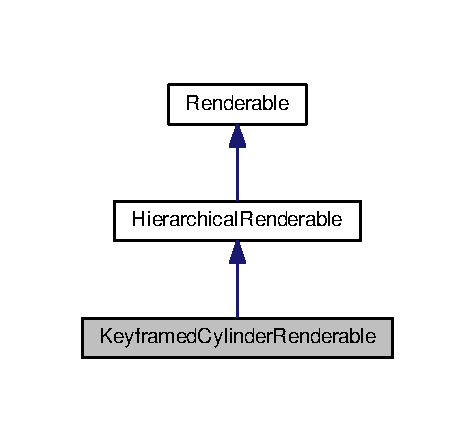
\includegraphics[width=228pt]{classKeyframedCylinderRenderable__inherit__graph}
\end{center}
\end{figure}


Collaboration diagram for Keyframed\+Cylinder\+Renderable\+:\nopagebreak
\begin{figure}[H]
\begin{center}
\leavevmode
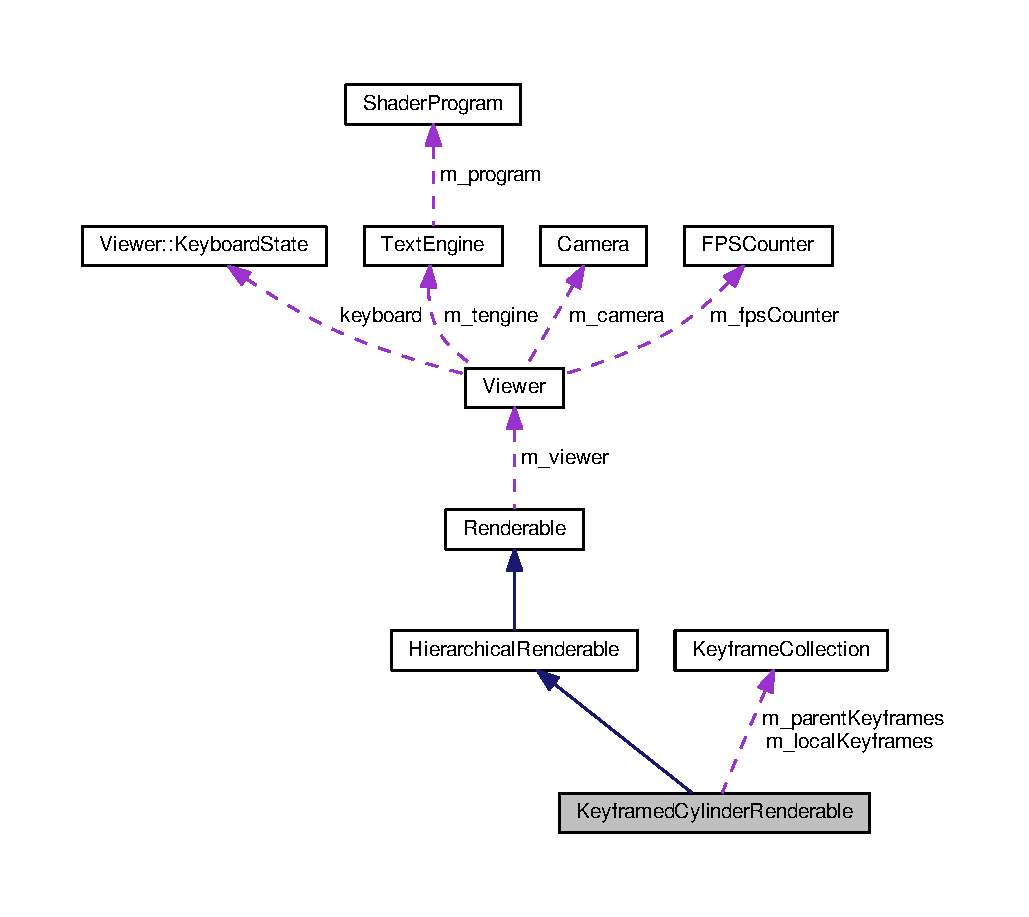
\includegraphics[width=350pt]{classKeyframedCylinderRenderable__coll__graph}
\end{center}
\end{figure}
\subsection*{Public Member Functions}
\begin{DoxyCompactItemize}
\item 
\hyperlink{classKeyframedCylinderRenderable_a0ce1e2ce884579462524de5d60bc8200}{$\sim$\+Keyframed\+Cylinder\+Renderable} ()
\item 
\hyperlink{classKeyframedCylinderRenderable_abb362bfe0ad89b97e1a5657da6562f85}{Keyframed\+Cylinder\+Renderable} (\hyperlink{ShaderProgram_8hpp_af8e4af1ad4c53875ee5d32ab7e1f4966}{Shader\+Program\+Ptr} program)
\item 
void \hyperlink{classKeyframedCylinderRenderable_a15d31ab79223c27b090e891f078ac64b}{add\+Local\+Transform\+Keyframe} (const \hyperlink{classGeometricTransformation}{Geometric\+Transformation} \&transformation, float time)
\begin{DoxyCompactList}\small\item\em Add a keyframe for the local transformation of the renderable. \end{DoxyCompactList}\item 
void \hyperlink{classKeyframedCylinderRenderable_ae635ccde0bfc30285b5bd3f47a24b9ad}{add\+Parent\+Transform\+Keyframe} (const \hyperlink{classGeometricTransformation}{Geometric\+Transformation} \&transformation, float time)
\begin{DoxyCompactList}\small\item\em Add a keyframe for the parent transformation of the renderable. \end{DoxyCompactList}\end{DoxyCompactItemize}
\subsection*{Private Member Functions}
\begin{DoxyCompactItemize}
\item 
void \hyperlink{classKeyframedCylinderRenderable_abbfc6deaafd95aa58feb2c08b22d1050}{do\+\_\+draw} ()
\begin{DoxyCompactList}\small\item\em Draw virtual function. \end{DoxyCompactList}\item 
void \hyperlink{classKeyframedCylinderRenderable_a59d9e6dedbf2e4105c08a8b6516cdd56}{do\+\_\+animate} (float time)
\begin{DoxyCompactList}\small\item\em Animate virtual function. \end{DoxyCompactList}\end{DoxyCompactItemize}
\subsection*{Private Attributes}
\begin{DoxyCompactItemize}
\item 
std\+::vector$<$ glm\+::vec3 $>$ \hyperlink{classKeyframedCylinderRenderable_a6429ca81b8b337a5b2fdbf25e5a232d2}{m\+\_\+positions}
\item 
std\+::vector$<$ glm\+::vec4 $>$ \hyperlink{classKeyframedCylinderRenderable_a7e70c2f1e07d14372589ef88f16e7bcd}{m\+\_\+colors}
\item 
std\+::vector$<$ glm\+::vec3 $>$ \hyperlink{classKeyframedCylinderRenderable_a4d306f63513ee46874d65078fb041a52}{m\+\_\+normals}
\item 
\hyperlink{classKeyframeCollection}{Keyframe\+Collection} \hyperlink{classKeyframedCylinderRenderable_a8d821f7953d26700d2eb49ca4b66cc18}{m\+\_\+local\+Keyframes}
\item 
\hyperlink{classKeyframeCollection}{Keyframe\+Collection} \hyperlink{classKeyframedCylinderRenderable_afcb8c6b8048454621f6375a1eebb2ca1}{m\+\_\+parent\+Keyframes}
\item 
unsigned int \hyperlink{classKeyframedCylinderRenderable_ae72ab893df021692d8c4e4d8e7081931}{m\+\_\+p\+Buffer}
\item 
unsigned int \hyperlink{classKeyframedCylinderRenderable_afdf432acba934c57255874373f234875}{m\+\_\+c\+Buffer}
\item 
unsigned int \hyperlink{classKeyframedCylinderRenderable_a73db5a6ed8d7452244834ef396cb0279}{m\+\_\+n\+Buffer}
\end{DoxyCompactItemize}
\subsection*{Additional Inherited Members}


\subsection{Constructor \& Destructor Documentation}
\hypertarget{classKeyframedCylinderRenderable_a0ce1e2ce884579462524de5d60bc8200}{\index{Keyframed\+Cylinder\+Renderable@{Keyframed\+Cylinder\+Renderable}!````~Keyframed\+Cylinder\+Renderable@{$\sim$\+Keyframed\+Cylinder\+Renderable}}
\index{````~Keyframed\+Cylinder\+Renderable@{$\sim$\+Keyframed\+Cylinder\+Renderable}!Keyframed\+Cylinder\+Renderable@{Keyframed\+Cylinder\+Renderable}}
\subsubsection[{$\sim$\+Keyframed\+Cylinder\+Renderable}]{\setlength{\rightskip}{0pt plus 5cm}Keyframed\+Cylinder\+Renderable\+::$\sim$\+Keyframed\+Cylinder\+Renderable (
\begin{DoxyParamCaption}
{}
\end{DoxyParamCaption}
)}}\label{classKeyframedCylinderRenderable_a0ce1e2ce884579462524de5d60bc8200}
\hypertarget{classKeyframedCylinderRenderable_abb362bfe0ad89b97e1a5657da6562f85}{\index{Keyframed\+Cylinder\+Renderable@{Keyframed\+Cylinder\+Renderable}!Keyframed\+Cylinder\+Renderable@{Keyframed\+Cylinder\+Renderable}}
\index{Keyframed\+Cylinder\+Renderable@{Keyframed\+Cylinder\+Renderable}!Keyframed\+Cylinder\+Renderable@{Keyframed\+Cylinder\+Renderable}}
\subsubsection[{Keyframed\+Cylinder\+Renderable}]{\setlength{\rightskip}{0pt plus 5cm}Keyframed\+Cylinder\+Renderable\+::\+Keyframed\+Cylinder\+Renderable (
\begin{DoxyParamCaption}
\item[{{\bf Shader\+Program\+Ptr}}]{program}
\end{DoxyParamCaption}
)}}\label{classKeyframedCylinderRenderable_abb362bfe0ad89b97e1a5657da6562f85}


\subsection{Member Function Documentation}
\hypertarget{classKeyframedCylinderRenderable_a15d31ab79223c27b090e891f078ac64b}{\index{Keyframed\+Cylinder\+Renderable@{Keyframed\+Cylinder\+Renderable}!add\+Local\+Transform\+Keyframe@{add\+Local\+Transform\+Keyframe}}
\index{add\+Local\+Transform\+Keyframe@{add\+Local\+Transform\+Keyframe}!Keyframed\+Cylinder\+Renderable@{Keyframed\+Cylinder\+Renderable}}
\subsubsection[{add\+Local\+Transform\+Keyframe}]{\setlength{\rightskip}{0pt plus 5cm}void Keyframed\+Cylinder\+Renderable\+::add\+Local\+Transform\+Keyframe (
\begin{DoxyParamCaption}
\item[{const {\bf Geometric\+Transformation} \&}]{transformation, }
\item[{float}]{time}
\end{DoxyParamCaption}
)}}\label{classKeyframedCylinderRenderable_a15d31ab79223c27b090e891f078ac64b}
Add a keyframe to m\+\_\+local\+Keyframes described by a geometric transformation and a time. 
\begin{DoxyParams}{Parameters}
{\em transformation} & The geometric transformation of the keyframe. \\
\hline
{\em time} & The time of the keyframe. \\
\hline
\end{DoxyParams}
\hypertarget{classKeyframedCylinderRenderable_ae635ccde0bfc30285b5bd3f47a24b9ad}{\index{Keyframed\+Cylinder\+Renderable@{Keyframed\+Cylinder\+Renderable}!add\+Parent\+Transform\+Keyframe@{add\+Parent\+Transform\+Keyframe}}
\index{add\+Parent\+Transform\+Keyframe@{add\+Parent\+Transform\+Keyframe}!Keyframed\+Cylinder\+Renderable@{Keyframed\+Cylinder\+Renderable}}
\subsubsection[{add\+Parent\+Transform\+Keyframe}]{\setlength{\rightskip}{0pt plus 5cm}void Keyframed\+Cylinder\+Renderable\+::add\+Parent\+Transform\+Keyframe (
\begin{DoxyParamCaption}
\item[{const {\bf Geometric\+Transformation} \&}]{transformation, }
\item[{float}]{time}
\end{DoxyParamCaption}
)}}\label{classKeyframedCylinderRenderable_ae635ccde0bfc30285b5bd3f47a24b9ad}
Add a keyframe to m\+\_\+parent\+Keyframes described by a geometric transformation and a time. 
\begin{DoxyParams}{Parameters}
{\em transformation} & The geometric transformation of the keyframe. \\
\hline
{\em time} & The time of the keyframe. \\
\hline
\end{DoxyParams}
\hypertarget{classKeyframedCylinderRenderable_a59d9e6dedbf2e4105c08a8b6516cdd56}{\index{Keyframed\+Cylinder\+Renderable@{Keyframed\+Cylinder\+Renderable}!do\+\_\+animate@{do\+\_\+animate}}
\index{do\+\_\+animate@{do\+\_\+animate}!Keyframed\+Cylinder\+Renderable@{Keyframed\+Cylinder\+Renderable}}
\subsubsection[{do\+\_\+animate}]{\setlength{\rightskip}{0pt plus 5cm}void Keyframed\+Cylinder\+Renderable\+::do\+\_\+animate (
\begin{DoxyParamCaption}
\item[{float}]{time}
\end{DoxyParamCaption}
)\hspace{0.3cm}{\ttfamily [private]}, {\ttfamily [virtual]}}}\label{classKeyframedCylinderRenderable_a59d9e6dedbf2e4105c08a8b6516cdd56}
Implementation to animate this renderable. 
\begin{DoxyParams}{Parameters}
{\em time} & The current simulation time. \\
\hline
\end{DoxyParams}


Implements \hyperlink{classRenderable_aa5206322555c9dece40b21e797629b34}{Renderable}.

\hypertarget{classKeyframedCylinderRenderable_abbfc6deaafd95aa58feb2c08b22d1050}{\index{Keyframed\+Cylinder\+Renderable@{Keyframed\+Cylinder\+Renderable}!do\+\_\+draw@{do\+\_\+draw}}
\index{do\+\_\+draw@{do\+\_\+draw}!Keyframed\+Cylinder\+Renderable@{Keyframed\+Cylinder\+Renderable}}
\subsubsection[{do\+\_\+draw}]{\setlength{\rightskip}{0pt plus 5cm}void Keyframed\+Cylinder\+Renderable\+::do\+\_\+draw (
\begin{DoxyParamCaption}
{}
\end{DoxyParamCaption}
)\hspace{0.3cm}{\ttfamily [private]}, {\ttfamily [virtual]}}}\label{classKeyframedCylinderRenderable_abbfc6deaafd95aa58feb2c08b22d1050}
Implementation to draw this renderable. 

Implements \hyperlink{classRenderable_a98ab6308c1d2b56dacda7c435fb38d5b}{Renderable}.



\subsection{Member Data Documentation}
\hypertarget{classKeyframedCylinderRenderable_afdf432acba934c57255874373f234875}{\index{Keyframed\+Cylinder\+Renderable@{Keyframed\+Cylinder\+Renderable}!m\+\_\+c\+Buffer@{m\+\_\+c\+Buffer}}
\index{m\+\_\+c\+Buffer@{m\+\_\+c\+Buffer}!Keyframed\+Cylinder\+Renderable@{Keyframed\+Cylinder\+Renderable}}
\subsubsection[{m\+\_\+c\+Buffer}]{\setlength{\rightskip}{0pt plus 5cm}unsigned int Keyframed\+Cylinder\+Renderable\+::m\+\_\+c\+Buffer\hspace{0.3cm}{\ttfamily [private]}}}\label{classKeyframedCylinderRenderable_afdf432acba934c57255874373f234875}
\hypertarget{classKeyframedCylinderRenderable_a7e70c2f1e07d14372589ef88f16e7bcd}{\index{Keyframed\+Cylinder\+Renderable@{Keyframed\+Cylinder\+Renderable}!m\+\_\+colors@{m\+\_\+colors}}
\index{m\+\_\+colors@{m\+\_\+colors}!Keyframed\+Cylinder\+Renderable@{Keyframed\+Cylinder\+Renderable}}
\subsubsection[{m\+\_\+colors}]{\setlength{\rightskip}{0pt plus 5cm}std\+::vector$<$ glm\+::vec4 $>$ Keyframed\+Cylinder\+Renderable\+::m\+\_\+colors\hspace{0.3cm}{\ttfamily [private]}}}\label{classKeyframedCylinderRenderable_a7e70c2f1e07d14372589ef88f16e7bcd}
\hypertarget{classKeyframedCylinderRenderable_a8d821f7953d26700d2eb49ca4b66cc18}{\index{Keyframed\+Cylinder\+Renderable@{Keyframed\+Cylinder\+Renderable}!m\+\_\+local\+Keyframes@{m\+\_\+local\+Keyframes}}
\index{m\+\_\+local\+Keyframes@{m\+\_\+local\+Keyframes}!Keyframed\+Cylinder\+Renderable@{Keyframed\+Cylinder\+Renderable}}
\subsubsection[{m\+\_\+local\+Keyframes}]{\setlength{\rightskip}{0pt plus 5cm}{\bf Keyframe\+Collection} Keyframed\+Cylinder\+Renderable\+::m\+\_\+local\+Keyframes\hspace{0.3cm}{\ttfamily [private]}}}\label{classKeyframedCylinderRenderable_a8d821f7953d26700d2eb49ca4b66cc18}
A collection of keyframes for the local transformation of renderable. \hypertarget{classKeyframedCylinderRenderable_a73db5a6ed8d7452244834ef396cb0279}{\index{Keyframed\+Cylinder\+Renderable@{Keyframed\+Cylinder\+Renderable}!m\+\_\+n\+Buffer@{m\+\_\+n\+Buffer}}
\index{m\+\_\+n\+Buffer@{m\+\_\+n\+Buffer}!Keyframed\+Cylinder\+Renderable@{Keyframed\+Cylinder\+Renderable}}
\subsubsection[{m\+\_\+n\+Buffer}]{\setlength{\rightskip}{0pt plus 5cm}unsigned int Keyframed\+Cylinder\+Renderable\+::m\+\_\+n\+Buffer\hspace{0.3cm}{\ttfamily [private]}}}\label{classKeyframedCylinderRenderable_a73db5a6ed8d7452244834ef396cb0279}
\hypertarget{classKeyframedCylinderRenderable_a4d306f63513ee46874d65078fb041a52}{\index{Keyframed\+Cylinder\+Renderable@{Keyframed\+Cylinder\+Renderable}!m\+\_\+normals@{m\+\_\+normals}}
\index{m\+\_\+normals@{m\+\_\+normals}!Keyframed\+Cylinder\+Renderable@{Keyframed\+Cylinder\+Renderable}}
\subsubsection[{m\+\_\+normals}]{\setlength{\rightskip}{0pt plus 5cm}std\+::vector$<$ glm\+::vec3 $>$ Keyframed\+Cylinder\+Renderable\+::m\+\_\+normals\hspace{0.3cm}{\ttfamily [private]}}}\label{classKeyframedCylinderRenderable_a4d306f63513ee46874d65078fb041a52}
\hypertarget{classKeyframedCylinderRenderable_afcb8c6b8048454621f6375a1eebb2ca1}{\index{Keyframed\+Cylinder\+Renderable@{Keyframed\+Cylinder\+Renderable}!m\+\_\+parent\+Keyframes@{m\+\_\+parent\+Keyframes}}
\index{m\+\_\+parent\+Keyframes@{m\+\_\+parent\+Keyframes}!Keyframed\+Cylinder\+Renderable@{Keyframed\+Cylinder\+Renderable}}
\subsubsection[{m\+\_\+parent\+Keyframes}]{\setlength{\rightskip}{0pt plus 5cm}{\bf Keyframe\+Collection} Keyframed\+Cylinder\+Renderable\+::m\+\_\+parent\+Keyframes\hspace{0.3cm}{\ttfamily [private]}}}\label{classKeyframedCylinderRenderable_afcb8c6b8048454621f6375a1eebb2ca1}
A collection of keyframes for the parent transformation of renderable. \hypertarget{classKeyframedCylinderRenderable_ae72ab893df021692d8c4e4d8e7081931}{\index{Keyframed\+Cylinder\+Renderable@{Keyframed\+Cylinder\+Renderable}!m\+\_\+p\+Buffer@{m\+\_\+p\+Buffer}}
\index{m\+\_\+p\+Buffer@{m\+\_\+p\+Buffer}!Keyframed\+Cylinder\+Renderable@{Keyframed\+Cylinder\+Renderable}}
\subsubsection[{m\+\_\+p\+Buffer}]{\setlength{\rightskip}{0pt plus 5cm}unsigned int Keyframed\+Cylinder\+Renderable\+::m\+\_\+p\+Buffer\hspace{0.3cm}{\ttfamily [private]}}}\label{classKeyframedCylinderRenderable_ae72ab893df021692d8c4e4d8e7081931}
\hypertarget{classKeyframedCylinderRenderable_a6429ca81b8b337a5b2fdbf25e5a232d2}{\index{Keyframed\+Cylinder\+Renderable@{Keyframed\+Cylinder\+Renderable}!m\+\_\+positions@{m\+\_\+positions}}
\index{m\+\_\+positions@{m\+\_\+positions}!Keyframed\+Cylinder\+Renderable@{Keyframed\+Cylinder\+Renderable}}
\subsubsection[{m\+\_\+positions}]{\setlength{\rightskip}{0pt plus 5cm}std\+::vector$<$ glm\+::vec3 $>$ Keyframed\+Cylinder\+Renderable\+::m\+\_\+positions\hspace{0.3cm}{\ttfamily [private]}}}\label{classKeyframedCylinderRenderable_a6429ca81b8b337a5b2fdbf25e5a232d2}


The documentation for this class was generated from the following file\+:\begin{DoxyCompactItemize}
\item 
/home/chardon/\+Depot/ensimag/2\+A\+\_\+\+G3\+D/practicals/teacher\+Source/include/\hyperlink{KeyframedCylinderRenderable_8hpp}{Keyframed\+Cylinder\+Renderable.\+hpp}\end{DoxyCompactItemize}

\hypertarget{classLightedCubeRenderable}{\section{Lighted\+Cube\+Renderable Class Reference}
\label{classLightedCubeRenderable}\index{Lighted\+Cube\+Renderable@{Lighted\+Cube\+Renderable}}
}


{\ttfamily \#include $<$Lighted\+Cube\+Renderable.\+hpp$>$}



Inheritance diagram for Lighted\+Cube\+Renderable\+:\nopagebreak
\begin{figure}[H]
\begin{center}
\leavevmode
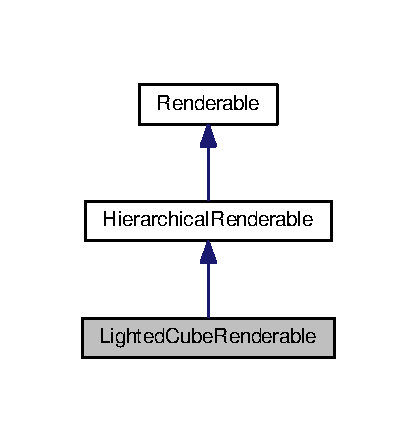
\includegraphics[width=200pt]{classLightedCubeRenderable__inherit__graph}
\end{center}
\end{figure}


Collaboration diagram for Lighted\+Cube\+Renderable\+:\nopagebreak
\begin{figure}[H]
\begin{center}
\leavevmode
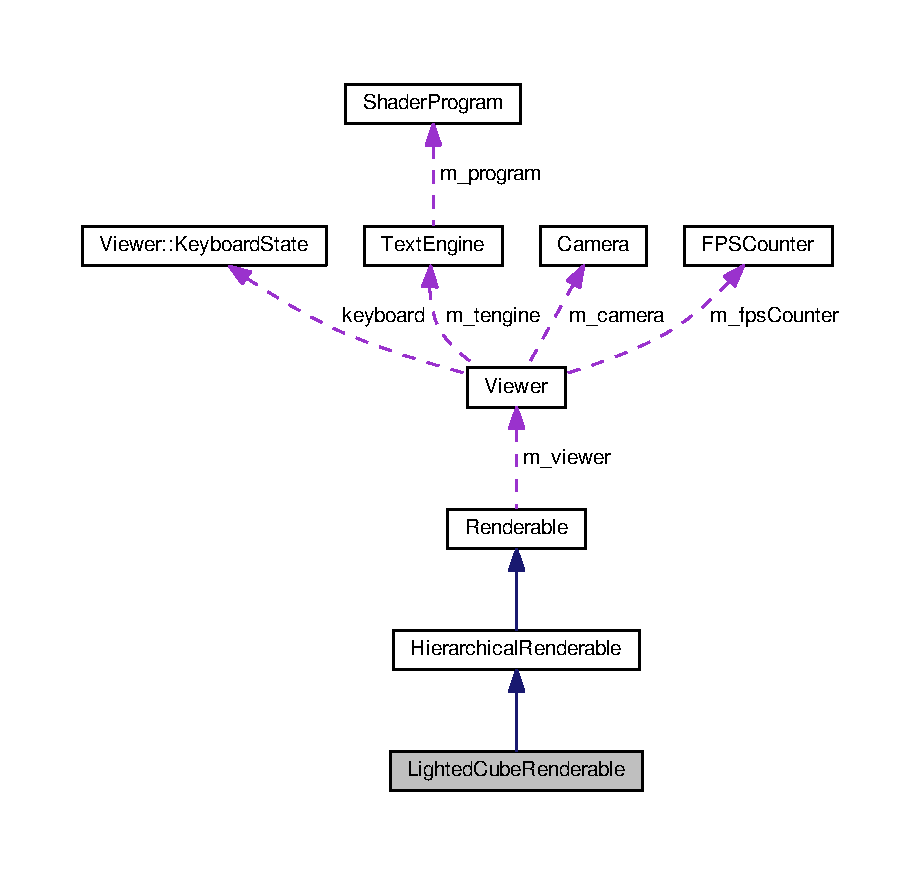
\includegraphics[width=350pt]{classLightedCubeRenderable__coll__graph}
\end{center}
\end{figure}
\subsection*{Public Member Functions}
\begin{DoxyCompactItemize}
\item 
\hyperlink{classLightedCubeRenderable_a5fa09ed9225574f38bae4620f7b38a93}{$\sim$\+Lighted\+Cube\+Renderable} ()
\item 
\hyperlink{classLightedCubeRenderable_a4ed004e7c6705115eb0cfc923d7d4323}{Lighted\+Cube\+Renderable} (\hyperlink{ShaderProgram_8hpp_af8e4af1ad4c53875ee5d32ab7e1f4966}{Shader\+Program\+Ptr} program)
\item 
void \hyperlink{classLightedCubeRenderable_a6dbf380a735cd69da08e80cd506ca7a3}{set\+Material} (const \hyperlink{Material_8hpp_a1d47cd05ca683e287435cf0b363fbfe1}{Material\+Ptr} \&material)
\end{DoxyCompactItemize}
\subsection*{Private Member Functions}
\begin{DoxyCompactItemize}
\item 
void \hyperlink{classLightedCubeRenderable_a62c74cad13c77f9442a8baab0c7d156c}{do\+\_\+draw} ()
\begin{DoxyCompactList}\small\item\em Draw virtual function. \end{DoxyCompactList}\item 
void \hyperlink{classLightedCubeRenderable_a2888876e6b826899dfe0611c0021b161}{do\+\_\+animate} (float time)
\begin{DoxyCompactList}\small\item\em Animate virtual function. \end{DoxyCompactList}\end{DoxyCompactItemize}
\subsection*{Private Attributes}
\begin{DoxyCompactItemize}
\item 
std\+::vector$<$ glm\+::vec3 $>$ \hyperlink{classLightedCubeRenderable_a0c0c5eb370f23cabfd1a683d784559af}{m\+\_\+positions}
\item 
std\+::vector$<$ glm\+::vec4 $>$ \hyperlink{classLightedCubeRenderable_a8d300c68f52441ea4b0b8633cdb80a2c}{m\+\_\+colors}
\item 
std\+::vector$<$ glm\+::vec3 $>$ \hyperlink{classLightedCubeRenderable_af2d85e3194b02e6f94004f0cd08195f9}{m\+\_\+normals}
\item 
unsigned int \hyperlink{classLightedCubeRenderable_a9454b080496e7ceb563615c1fa14be9b}{m\+\_\+p\+Buffer}
\item 
unsigned int \hyperlink{classLightedCubeRenderable_aab6ae791b76f419fc6f0255718cc3ab1}{m\+\_\+c\+Buffer}
\item 
unsigned int \hyperlink{classLightedCubeRenderable_a65b42742eca437c5d84b75137abafbd7}{m\+\_\+n\+Buffer}
\item 
\hyperlink{Material_8hpp_a1d47cd05ca683e287435cf0b363fbfe1}{Material\+Ptr} \hyperlink{classLightedCubeRenderable_a06c8156cc469df88e25ee2cdeb00fa4a}{m\+\_\+material}
\end{DoxyCompactItemize}
\subsection*{Additional Inherited Members}


\subsection{Constructor \& Destructor Documentation}
\hypertarget{classLightedCubeRenderable_a5fa09ed9225574f38bae4620f7b38a93}{\index{Lighted\+Cube\+Renderable@{Lighted\+Cube\+Renderable}!````~Lighted\+Cube\+Renderable@{$\sim$\+Lighted\+Cube\+Renderable}}
\index{````~Lighted\+Cube\+Renderable@{$\sim$\+Lighted\+Cube\+Renderable}!Lighted\+Cube\+Renderable@{Lighted\+Cube\+Renderable}}
\subsubsection[{$\sim$\+Lighted\+Cube\+Renderable}]{\setlength{\rightskip}{0pt plus 5cm}Lighted\+Cube\+Renderable\+::$\sim$\+Lighted\+Cube\+Renderable (
\begin{DoxyParamCaption}
{}
\end{DoxyParamCaption}
)}}\label{classLightedCubeRenderable_a5fa09ed9225574f38bae4620f7b38a93}
\hypertarget{classLightedCubeRenderable_a4ed004e7c6705115eb0cfc923d7d4323}{\index{Lighted\+Cube\+Renderable@{Lighted\+Cube\+Renderable}!Lighted\+Cube\+Renderable@{Lighted\+Cube\+Renderable}}
\index{Lighted\+Cube\+Renderable@{Lighted\+Cube\+Renderable}!Lighted\+Cube\+Renderable@{Lighted\+Cube\+Renderable}}
\subsubsection[{Lighted\+Cube\+Renderable}]{\setlength{\rightskip}{0pt plus 5cm}Lighted\+Cube\+Renderable\+::\+Lighted\+Cube\+Renderable (
\begin{DoxyParamCaption}
\item[{{\bf Shader\+Program\+Ptr}}]{program}
\end{DoxyParamCaption}
)}}\label{classLightedCubeRenderable_a4ed004e7c6705115eb0cfc923d7d4323}


\subsection{Member Function Documentation}
\hypertarget{classLightedCubeRenderable_a2888876e6b826899dfe0611c0021b161}{\index{Lighted\+Cube\+Renderable@{Lighted\+Cube\+Renderable}!do\+\_\+animate@{do\+\_\+animate}}
\index{do\+\_\+animate@{do\+\_\+animate}!Lighted\+Cube\+Renderable@{Lighted\+Cube\+Renderable}}
\subsubsection[{do\+\_\+animate}]{\setlength{\rightskip}{0pt plus 5cm}void Lighted\+Cube\+Renderable\+::do\+\_\+animate (
\begin{DoxyParamCaption}
\item[{float}]{time}
\end{DoxyParamCaption}
)\hspace{0.3cm}{\ttfamily [private]}, {\ttfamily [virtual]}}}\label{classLightedCubeRenderable_a2888876e6b826899dfe0611c0021b161}
Implementation to animate this renderable. 
\begin{DoxyParams}{Parameters}
{\em time} & The current simulation time. \\
\hline
\end{DoxyParams}


Implements \hyperlink{classRenderable_aa5206322555c9dece40b21e797629b34}{Renderable}.

\hypertarget{classLightedCubeRenderable_a62c74cad13c77f9442a8baab0c7d156c}{\index{Lighted\+Cube\+Renderable@{Lighted\+Cube\+Renderable}!do\+\_\+draw@{do\+\_\+draw}}
\index{do\+\_\+draw@{do\+\_\+draw}!Lighted\+Cube\+Renderable@{Lighted\+Cube\+Renderable}}
\subsubsection[{do\+\_\+draw}]{\setlength{\rightskip}{0pt plus 5cm}void Lighted\+Cube\+Renderable\+::do\+\_\+draw (
\begin{DoxyParamCaption}
{}
\end{DoxyParamCaption}
)\hspace{0.3cm}{\ttfamily [private]}, {\ttfamily [virtual]}}}\label{classLightedCubeRenderable_a62c74cad13c77f9442a8baab0c7d156c}
Implementation to draw this renderable. 

Implements \hyperlink{classRenderable_a98ab6308c1d2b56dacda7c435fb38d5b}{Renderable}.

\hypertarget{classLightedCubeRenderable_a6dbf380a735cd69da08e80cd506ca7a3}{\index{Lighted\+Cube\+Renderable@{Lighted\+Cube\+Renderable}!set\+Material@{set\+Material}}
\index{set\+Material@{set\+Material}!Lighted\+Cube\+Renderable@{Lighted\+Cube\+Renderable}}
\subsubsection[{set\+Material}]{\setlength{\rightskip}{0pt plus 5cm}void Lighted\+Cube\+Renderable\+::set\+Material (
\begin{DoxyParamCaption}
\item[{const {\bf Material\+Ptr} \&}]{material}
\end{DoxyParamCaption}
)}}\label{classLightedCubeRenderable_a6dbf380a735cd69da08e80cd506ca7a3}


\subsection{Member Data Documentation}
\hypertarget{classLightedCubeRenderable_aab6ae791b76f419fc6f0255718cc3ab1}{\index{Lighted\+Cube\+Renderable@{Lighted\+Cube\+Renderable}!m\+\_\+c\+Buffer@{m\+\_\+c\+Buffer}}
\index{m\+\_\+c\+Buffer@{m\+\_\+c\+Buffer}!Lighted\+Cube\+Renderable@{Lighted\+Cube\+Renderable}}
\subsubsection[{m\+\_\+c\+Buffer}]{\setlength{\rightskip}{0pt plus 5cm}unsigned int Lighted\+Cube\+Renderable\+::m\+\_\+c\+Buffer\hspace{0.3cm}{\ttfamily [private]}}}\label{classLightedCubeRenderable_aab6ae791b76f419fc6f0255718cc3ab1}
\hypertarget{classLightedCubeRenderable_a8d300c68f52441ea4b0b8633cdb80a2c}{\index{Lighted\+Cube\+Renderable@{Lighted\+Cube\+Renderable}!m\+\_\+colors@{m\+\_\+colors}}
\index{m\+\_\+colors@{m\+\_\+colors}!Lighted\+Cube\+Renderable@{Lighted\+Cube\+Renderable}}
\subsubsection[{m\+\_\+colors}]{\setlength{\rightskip}{0pt plus 5cm}std\+::vector$<$ glm\+::vec4 $>$ Lighted\+Cube\+Renderable\+::m\+\_\+colors\hspace{0.3cm}{\ttfamily [private]}}}\label{classLightedCubeRenderable_a8d300c68f52441ea4b0b8633cdb80a2c}
\hypertarget{classLightedCubeRenderable_a06c8156cc469df88e25ee2cdeb00fa4a}{\index{Lighted\+Cube\+Renderable@{Lighted\+Cube\+Renderable}!m\+\_\+material@{m\+\_\+material}}
\index{m\+\_\+material@{m\+\_\+material}!Lighted\+Cube\+Renderable@{Lighted\+Cube\+Renderable}}
\subsubsection[{m\+\_\+material}]{\setlength{\rightskip}{0pt plus 5cm}{\bf Material\+Ptr} Lighted\+Cube\+Renderable\+::m\+\_\+material\hspace{0.3cm}{\ttfamily [private]}}}\label{classLightedCubeRenderable_a06c8156cc469df88e25ee2cdeb00fa4a}
\hypertarget{classLightedCubeRenderable_a65b42742eca437c5d84b75137abafbd7}{\index{Lighted\+Cube\+Renderable@{Lighted\+Cube\+Renderable}!m\+\_\+n\+Buffer@{m\+\_\+n\+Buffer}}
\index{m\+\_\+n\+Buffer@{m\+\_\+n\+Buffer}!Lighted\+Cube\+Renderable@{Lighted\+Cube\+Renderable}}
\subsubsection[{m\+\_\+n\+Buffer}]{\setlength{\rightskip}{0pt plus 5cm}unsigned int Lighted\+Cube\+Renderable\+::m\+\_\+n\+Buffer\hspace{0.3cm}{\ttfamily [private]}}}\label{classLightedCubeRenderable_a65b42742eca437c5d84b75137abafbd7}
\hypertarget{classLightedCubeRenderable_af2d85e3194b02e6f94004f0cd08195f9}{\index{Lighted\+Cube\+Renderable@{Lighted\+Cube\+Renderable}!m\+\_\+normals@{m\+\_\+normals}}
\index{m\+\_\+normals@{m\+\_\+normals}!Lighted\+Cube\+Renderable@{Lighted\+Cube\+Renderable}}
\subsubsection[{m\+\_\+normals}]{\setlength{\rightskip}{0pt plus 5cm}std\+::vector$<$ glm\+::vec3 $>$ Lighted\+Cube\+Renderable\+::m\+\_\+normals\hspace{0.3cm}{\ttfamily [private]}}}\label{classLightedCubeRenderable_af2d85e3194b02e6f94004f0cd08195f9}
\hypertarget{classLightedCubeRenderable_a9454b080496e7ceb563615c1fa14be9b}{\index{Lighted\+Cube\+Renderable@{Lighted\+Cube\+Renderable}!m\+\_\+p\+Buffer@{m\+\_\+p\+Buffer}}
\index{m\+\_\+p\+Buffer@{m\+\_\+p\+Buffer}!Lighted\+Cube\+Renderable@{Lighted\+Cube\+Renderable}}
\subsubsection[{m\+\_\+p\+Buffer}]{\setlength{\rightskip}{0pt plus 5cm}unsigned int Lighted\+Cube\+Renderable\+::m\+\_\+p\+Buffer\hspace{0.3cm}{\ttfamily [private]}}}\label{classLightedCubeRenderable_a9454b080496e7ceb563615c1fa14be9b}
\hypertarget{classLightedCubeRenderable_a0c0c5eb370f23cabfd1a683d784559af}{\index{Lighted\+Cube\+Renderable@{Lighted\+Cube\+Renderable}!m\+\_\+positions@{m\+\_\+positions}}
\index{m\+\_\+positions@{m\+\_\+positions}!Lighted\+Cube\+Renderable@{Lighted\+Cube\+Renderable}}
\subsubsection[{m\+\_\+positions}]{\setlength{\rightskip}{0pt plus 5cm}std\+::vector$<$ glm\+::vec3 $>$ Lighted\+Cube\+Renderable\+::m\+\_\+positions\hspace{0.3cm}{\ttfamily [private]}}}\label{classLightedCubeRenderable_a0c0c5eb370f23cabfd1a683d784559af}


The documentation for this class was generated from the following file\+:\begin{DoxyCompactItemize}
\item 
/home/chardon/\+Depot/ensimag/2\+A\+\_\+\+G3\+D/practicals/teacher\+Source/include/lighting/\hyperlink{LightedCubeRenderable_8hpp}{Lighted\+Cube\+Renderable.\+hpp}\end{DoxyCompactItemize}

\hypertarget{classLightedCylinderRenderable}{\section{Lighted\+Cylinder\+Renderable Class Reference}
\label{classLightedCylinderRenderable}\index{Lighted\+Cylinder\+Renderable@{Lighted\+Cylinder\+Renderable}}
}


{\ttfamily \#include $<$Lighted\+Cylinder\+Renderable.\+hpp$>$}



Inheritance diagram for Lighted\+Cylinder\+Renderable\+:\nopagebreak
\begin{figure}[H]
\begin{center}
\leavevmode
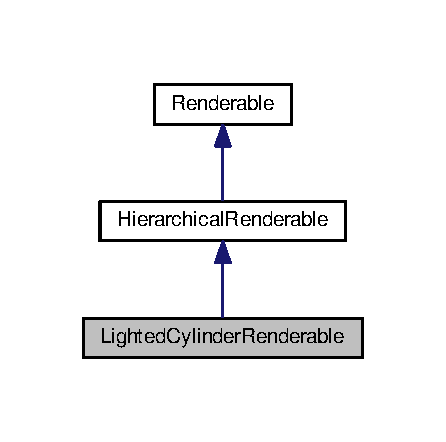
\includegraphics[width=214pt]{classLightedCylinderRenderable__inherit__graph}
\end{center}
\end{figure}


Collaboration diagram for Lighted\+Cylinder\+Renderable\+:\nopagebreak
\begin{figure}[H]
\begin{center}
\leavevmode
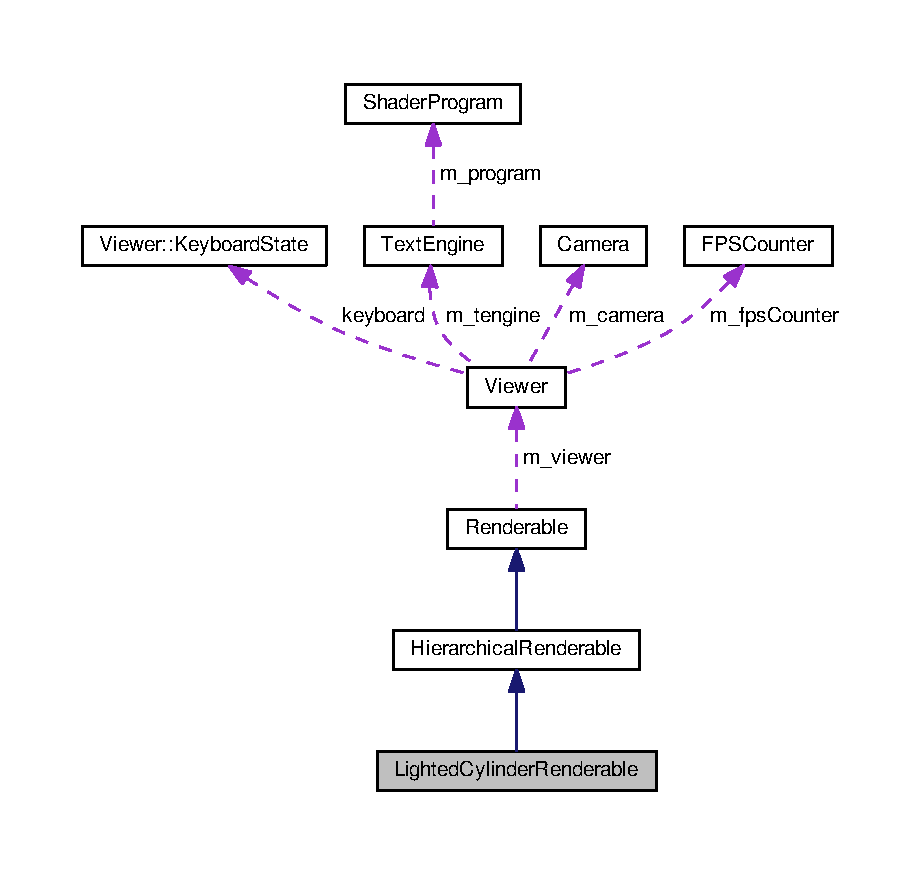
\includegraphics[width=350pt]{classLightedCylinderRenderable__coll__graph}
\end{center}
\end{figure}
\subsection*{Public Member Functions}
\begin{DoxyCompactItemize}
\item 
\hyperlink{classLightedCylinderRenderable_a099f169da178f08e3b3e1c39873ff54e}{$\sim$\+Lighted\+Cylinder\+Renderable} ()
\item 
\hyperlink{classLightedCylinderRenderable_a77e38146024a45063d5874ac176bf84f}{Lighted\+Cylinder\+Renderable} (\hyperlink{ShaderProgram_8hpp_af8e4af1ad4c53875ee5d32ab7e1f4966}{Shader\+Program\+Ptr} program)
\item 
void \hyperlink{classLightedCylinderRenderable_af63ed94be5df5dc25a58c01b44a2e82d}{set\+Material} (const \hyperlink{Material_8hpp_a1d47cd05ca683e287435cf0b363fbfe1}{Material\+Ptr} \&material)
\end{DoxyCompactItemize}
\subsection*{Private Member Functions}
\begin{DoxyCompactItemize}
\item 
void \hyperlink{classLightedCylinderRenderable_a327da1ffb8ac46a01b4c8057ea532acb}{do\+\_\+draw} ()
\begin{DoxyCompactList}\small\item\em Draw virtual function. \end{DoxyCompactList}\item 
void \hyperlink{classLightedCylinderRenderable_a7ecf5b614bf6e98335e9b46edfc64e67}{do\+\_\+animate} (float time)
\begin{DoxyCompactList}\small\item\em Animate virtual function. \end{DoxyCompactList}\end{DoxyCompactItemize}
\subsection*{Private Attributes}
\begin{DoxyCompactItemize}
\item 
std\+::vector$<$ glm\+::vec3 $>$ \hyperlink{classLightedCylinderRenderable_af92700359498f5307fb416f641a9015d}{m\+\_\+positions}
\item 
std\+::vector$<$ glm\+::vec4 $>$ \hyperlink{classLightedCylinderRenderable_a33d59e3d7e08b0123102624da0caa396}{m\+\_\+colors}
\item 
std\+::vector$<$ glm\+::vec3 $>$ \hyperlink{classLightedCylinderRenderable_ae5305cb063f670b7c8943423b82f2d1f}{m\+\_\+normals}
\item 
unsigned int \hyperlink{classLightedCylinderRenderable_abf3d79539f561c684db8394bc489cf38}{m\+\_\+p\+Buffer}
\item 
unsigned int \hyperlink{classLightedCylinderRenderable_a2795079c02ff376e0b4a7e2507371d94}{m\+\_\+c\+Buffer}
\item 
unsigned int \hyperlink{classLightedCylinderRenderable_abb74e2395d504a3393ba2b59276bf361}{m\+\_\+n\+Buffer}
\item 
\hyperlink{Material_8hpp_a1d47cd05ca683e287435cf0b363fbfe1}{Material\+Ptr} \hyperlink{classLightedCylinderRenderable_a69203c5141f12784a61ab3cefb885b3f}{m\+\_\+material}
\end{DoxyCompactItemize}
\subsection*{Additional Inherited Members}


\subsection{Constructor \& Destructor Documentation}
\hypertarget{classLightedCylinderRenderable_a099f169da178f08e3b3e1c39873ff54e}{\index{Lighted\+Cylinder\+Renderable@{Lighted\+Cylinder\+Renderable}!````~Lighted\+Cylinder\+Renderable@{$\sim$\+Lighted\+Cylinder\+Renderable}}
\index{````~Lighted\+Cylinder\+Renderable@{$\sim$\+Lighted\+Cylinder\+Renderable}!Lighted\+Cylinder\+Renderable@{Lighted\+Cylinder\+Renderable}}
\subsubsection[{$\sim$\+Lighted\+Cylinder\+Renderable}]{\setlength{\rightskip}{0pt plus 5cm}Lighted\+Cylinder\+Renderable\+::$\sim$\+Lighted\+Cylinder\+Renderable (
\begin{DoxyParamCaption}
{}
\end{DoxyParamCaption}
)}}\label{classLightedCylinderRenderable_a099f169da178f08e3b3e1c39873ff54e}
\hypertarget{classLightedCylinderRenderable_a77e38146024a45063d5874ac176bf84f}{\index{Lighted\+Cylinder\+Renderable@{Lighted\+Cylinder\+Renderable}!Lighted\+Cylinder\+Renderable@{Lighted\+Cylinder\+Renderable}}
\index{Lighted\+Cylinder\+Renderable@{Lighted\+Cylinder\+Renderable}!Lighted\+Cylinder\+Renderable@{Lighted\+Cylinder\+Renderable}}
\subsubsection[{Lighted\+Cylinder\+Renderable}]{\setlength{\rightskip}{0pt plus 5cm}Lighted\+Cylinder\+Renderable\+::\+Lighted\+Cylinder\+Renderable (
\begin{DoxyParamCaption}
\item[{{\bf Shader\+Program\+Ptr}}]{program}
\end{DoxyParamCaption}
)}}\label{classLightedCylinderRenderable_a77e38146024a45063d5874ac176bf84f}


\subsection{Member Function Documentation}
\hypertarget{classLightedCylinderRenderable_a7ecf5b614bf6e98335e9b46edfc64e67}{\index{Lighted\+Cylinder\+Renderable@{Lighted\+Cylinder\+Renderable}!do\+\_\+animate@{do\+\_\+animate}}
\index{do\+\_\+animate@{do\+\_\+animate}!Lighted\+Cylinder\+Renderable@{Lighted\+Cylinder\+Renderable}}
\subsubsection[{do\+\_\+animate}]{\setlength{\rightskip}{0pt plus 5cm}void Lighted\+Cylinder\+Renderable\+::do\+\_\+animate (
\begin{DoxyParamCaption}
\item[{float}]{time}
\end{DoxyParamCaption}
)\hspace{0.3cm}{\ttfamily [private]}, {\ttfamily [virtual]}}}\label{classLightedCylinderRenderable_a7ecf5b614bf6e98335e9b46edfc64e67}
Implementation to animate this renderable. 
\begin{DoxyParams}{Parameters}
{\em time} & The current simulation time. \\
\hline
\end{DoxyParams}


Implements \hyperlink{classRenderable_aa5206322555c9dece40b21e797629b34}{Renderable}.

\hypertarget{classLightedCylinderRenderable_a327da1ffb8ac46a01b4c8057ea532acb}{\index{Lighted\+Cylinder\+Renderable@{Lighted\+Cylinder\+Renderable}!do\+\_\+draw@{do\+\_\+draw}}
\index{do\+\_\+draw@{do\+\_\+draw}!Lighted\+Cylinder\+Renderable@{Lighted\+Cylinder\+Renderable}}
\subsubsection[{do\+\_\+draw}]{\setlength{\rightskip}{0pt plus 5cm}void Lighted\+Cylinder\+Renderable\+::do\+\_\+draw (
\begin{DoxyParamCaption}
{}
\end{DoxyParamCaption}
)\hspace{0.3cm}{\ttfamily [private]}, {\ttfamily [virtual]}}}\label{classLightedCylinderRenderable_a327da1ffb8ac46a01b4c8057ea532acb}
Implementation to draw this renderable. 

Implements \hyperlink{classRenderable_a98ab6308c1d2b56dacda7c435fb38d5b}{Renderable}.

\hypertarget{classLightedCylinderRenderable_af63ed94be5df5dc25a58c01b44a2e82d}{\index{Lighted\+Cylinder\+Renderable@{Lighted\+Cylinder\+Renderable}!set\+Material@{set\+Material}}
\index{set\+Material@{set\+Material}!Lighted\+Cylinder\+Renderable@{Lighted\+Cylinder\+Renderable}}
\subsubsection[{set\+Material}]{\setlength{\rightskip}{0pt plus 5cm}void Lighted\+Cylinder\+Renderable\+::set\+Material (
\begin{DoxyParamCaption}
\item[{const {\bf Material\+Ptr} \&}]{material}
\end{DoxyParamCaption}
)}}\label{classLightedCylinderRenderable_af63ed94be5df5dc25a58c01b44a2e82d}


\subsection{Member Data Documentation}
\hypertarget{classLightedCylinderRenderable_a2795079c02ff376e0b4a7e2507371d94}{\index{Lighted\+Cylinder\+Renderable@{Lighted\+Cylinder\+Renderable}!m\+\_\+c\+Buffer@{m\+\_\+c\+Buffer}}
\index{m\+\_\+c\+Buffer@{m\+\_\+c\+Buffer}!Lighted\+Cylinder\+Renderable@{Lighted\+Cylinder\+Renderable}}
\subsubsection[{m\+\_\+c\+Buffer}]{\setlength{\rightskip}{0pt plus 5cm}unsigned int Lighted\+Cylinder\+Renderable\+::m\+\_\+c\+Buffer\hspace{0.3cm}{\ttfamily [private]}}}\label{classLightedCylinderRenderable_a2795079c02ff376e0b4a7e2507371d94}
\hypertarget{classLightedCylinderRenderable_a33d59e3d7e08b0123102624da0caa396}{\index{Lighted\+Cylinder\+Renderable@{Lighted\+Cylinder\+Renderable}!m\+\_\+colors@{m\+\_\+colors}}
\index{m\+\_\+colors@{m\+\_\+colors}!Lighted\+Cylinder\+Renderable@{Lighted\+Cylinder\+Renderable}}
\subsubsection[{m\+\_\+colors}]{\setlength{\rightskip}{0pt plus 5cm}std\+::vector$<$ glm\+::vec4 $>$ Lighted\+Cylinder\+Renderable\+::m\+\_\+colors\hspace{0.3cm}{\ttfamily [private]}}}\label{classLightedCylinderRenderable_a33d59e3d7e08b0123102624da0caa396}
\hypertarget{classLightedCylinderRenderable_a69203c5141f12784a61ab3cefb885b3f}{\index{Lighted\+Cylinder\+Renderable@{Lighted\+Cylinder\+Renderable}!m\+\_\+material@{m\+\_\+material}}
\index{m\+\_\+material@{m\+\_\+material}!Lighted\+Cylinder\+Renderable@{Lighted\+Cylinder\+Renderable}}
\subsubsection[{m\+\_\+material}]{\setlength{\rightskip}{0pt plus 5cm}{\bf Material\+Ptr} Lighted\+Cylinder\+Renderable\+::m\+\_\+material\hspace{0.3cm}{\ttfamily [private]}}}\label{classLightedCylinderRenderable_a69203c5141f12784a61ab3cefb885b3f}
\hypertarget{classLightedCylinderRenderable_abb74e2395d504a3393ba2b59276bf361}{\index{Lighted\+Cylinder\+Renderable@{Lighted\+Cylinder\+Renderable}!m\+\_\+n\+Buffer@{m\+\_\+n\+Buffer}}
\index{m\+\_\+n\+Buffer@{m\+\_\+n\+Buffer}!Lighted\+Cylinder\+Renderable@{Lighted\+Cylinder\+Renderable}}
\subsubsection[{m\+\_\+n\+Buffer}]{\setlength{\rightskip}{0pt plus 5cm}unsigned int Lighted\+Cylinder\+Renderable\+::m\+\_\+n\+Buffer\hspace{0.3cm}{\ttfamily [private]}}}\label{classLightedCylinderRenderable_abb74e2395d504a3393ba2b59276bf361}
\hypertarget{classLightedCylinderRenderable_ae5305cb063f670b7c8943423b82f2d1f}{\index{Lighted\+Cylinder\+Renderable@{Lighted\+Cylinder\+Renderable}!m\+\_\+normals@{m\+\_\+normals}}
\index{m\+\_\+normals@{m\+\_\+normals}!Lighted\+Cylinder\+Renderable@{Lighted\+Cylinder\+Renderable}}
\subsubsection[{m\+\_\+normals}]{\setlength{\rightskip}{0pt plus 5cm}std\+::vector$<$ glm\+::vec3 $>$ Lighted\+Cylinder\+Renderable\+::m\+\_\+normals\hspace{0.3cm}{\ttfamily [private]}}}\label{classLightedCylinderRenderable_ae5305cb063f670b7c8943423b82f2d1f}
\hypertarget{classLightedCylinderRenderable_abf3d79539f561c684db8394bc489cf38}{\index{Lighted\+Cylinder\+Renderable@{Lighted\+Cylinder\+Renderable}!m\+\_\+p\+Buffer@{m\+\_\+p\+Buffer}}
\index{m\+\_\+p\+Buffer@{m\+\_\+p\+Buffer}!Lighted\+Cylinder\+Renderable@{Lighted\+Cylinder\+Renderable}}
\subsubsection[{m\+\_\+p\+Buffer}]{\setlength{\rightskip}{0pt plus 5cm}unsigned int Lighted\+Cylinder\+Renderable\+::m\+\_\+p\+Buffer\hspace{0.3cm}{\ttfamily [private]}}}\label{classLightedCylinderRenderable_abf3d79539f561c684db8394bc489cf38}
\hypertarget{classLightedCylinderRenderable_af92700359498f5307fb416f641a9015d}{\index{Lighted\+Cylinder\+Renderable@{Lighted\+Cylinder\+Renderable}!m\+\_\+positions@{m\+\_\+positions}}
\index{m\+\_\+positions@{m\+\_\+positions}!Lighted\+Cylinder\+Renderable@{Lighted\+Cylinder\+Renderable}}
\subsubsection[{m\+\_\+positions}]{\setlength{\rightskip}{0pt plus 5cm}std\+::vector$<$ glm\+::vec3 $>$ Lighted\+Cylinder\+Renderable\+::m\+\_\+positions\hspace{0.3cm}{\ttfamily [private]}}}\label{classLightedCylinderRenderable_af92700359498f5307fb416f641a9015d}


The documentation for this class was generated from the following file\+:\begin{DoxyCompactItemize}
\item 
/home/chardon/\+Depot/ensimag/2\+A\+\_\+\+G3\+D/practicals/teacher\+Source/include/lighting/\hyperlink{LightedCylinderRenderable_8hpp}{Lighted\+Cylinder\+Renderable.\+hpp}\end{DoxyCompactItemize}

\hypertarget{classLightedMeshRenderable}{\section{Lighted\+Mesh\+Renderable Class Reference}
\label{classLightedMeshRenderable}\index{Lighted\+Mesh\+Renderable@{Lighted\+Mesh\+Renderable}}
}


{\ttfamily \#include $<$Lighted\+Mesh\+Renderable.\+hpp$>$}



Inheritance diagram for Lighted\+Mesh\+Renderable\+:\nopagebreak
\begin{figure}[H]
\begin{center}
\leavevmode
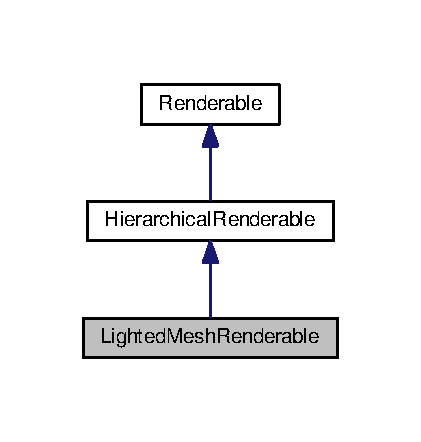
\includegraphics[width=202pt]{classLightedMeshRenderable__inherit__graph}
\end{center}
\end{figure}


Collaboration diagram for Lighted\+Mesh\+Renderable\+:\nopagebreak
\begin{figure}[H]
\begin{center}
\leavevmode
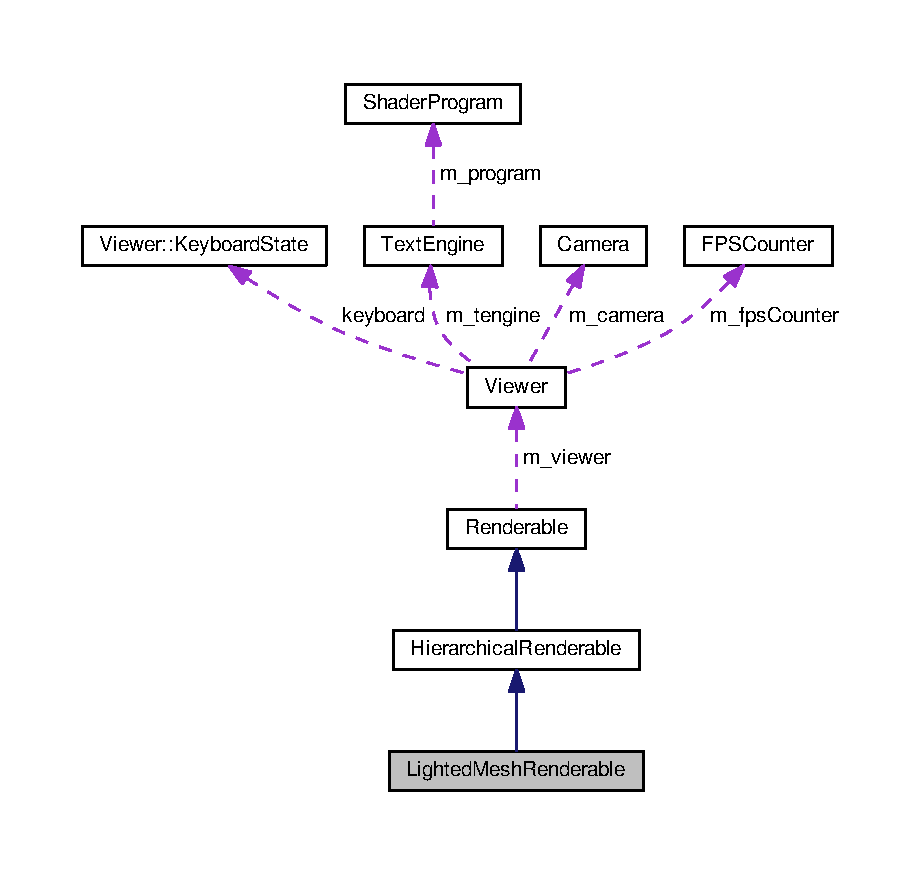
\includegraphics[width=350pt]{classLightedMeshRenderable__coll__graph}
\end{center}
\end{figure}
\subsection*{Public Member Functions}
\begin{DoxyCompactItemize}
\item 
\hyperlink{classLightedMeshRenderable_a9d63d77cb9fb570b7ff61b32b1d19367}{$\sim$\+Lighted\+Mesh\+Renderable} ()
\item 
\hyperlink{classLightedMeshRenderable_a1631f932be02e2df689ada7a79f6f77b}{Lighted\+Mesh\+Renderable} (\hyperlink{ShaderProgram_8hpp_af8e4af1ad4c53875ee5d32ab7e1f4966}{Shader\+Program\+Ptr} program, const std\+::string \&filename)
\item 
void \hyperlink{classLightedMeshRenderable_acbc08d68271c47c60c36dfa52e90b340}{set\+Material} (const \hyperlink{Material_8hpp_a1d47cd05ca683e287435cf0b363fbfe1}{Material\+Ptr} \&material)
\end{DoxyCompactItemize}
\subsection*{Private Member Functions}
\begin{DoxyCompactItemize}
\item 
void \hyperlink{classLightedMeshRenderable_a7e4e538e3f45818789f28924fd18a478}{do\+\_\+draw} ()
\begin{DoxyCompactList}\small\item\em Draw virtual function. \end{DoxyCompactList}\item 
void \hyperlink{classLightedMeshRenderable_aa22c64fe3f33f88c164ffa087c9ec71f}{do\+\_\+animate} (float time)
\begin{DoxyCompactList}\small\item\em Animate virtual function. \end{DoxyCompactList}\end{DoxyCompactItemize}
\subsection*{Private Attributes}
\begin{DoxyCompactItemize}
\item 
std\+::vector$<$ glm\+::vec3 $>$ \hyperlink{classLightedMeshRenderable_acc09c83711ed52719dce8ecb21402b73}{m\+\_\+positions}
\item 
std\+::vector$<$ glm\+::vec3 $>$ \hyperlink{classLightedMeshRenderable_a37b64e7bf9a9062aaad0aac05f04714c}{m\+\_\+normals}
\item 
std\+::vector$<$ glm\+::vec4 $>$ \hyperlink{classLightedMeshRenderable_ac22bb908efafa4720767615e7eab7bf9}{m\+\_\+colors}
\item 
std\+::vector$<$ unsigned int $>$ \hyperlink{classLightedMeshRenderable_af2bb140e6238e4740cb2b59efb431801}{m\+\_\+indices}
\item 
unsigned int \hyperlink{classLightedMeshRenderable_a1617b5e5bfddb4395ca27ab80271c915}{m\+\_\+p\+Buffer}
\item 
unsigned int \hyperlink{classLightedMeshRenderable_afd73d691c525f8b5d7f93aa65561f928}{m\+\_\+c\+Buffer}
\item 
unsigned int \hyperlink{classLightedMeshRenderable_a86a21c313ce8b7d1fff4bfbc7d60bfce}{m\+\_\+n\+Buffer}
\item 
unsigned int \hyperlink{classLightedMeshRenderable_adc7552281a74337733996a2812fe1fa6}{m\+\_\+i\+Buffer}
\item 
\hyperlink{Material_8hpp_a1d47cd05ca683e287435cf0b363fbfe1}{Material\+Ptr} \hyperlink{classLightedMeshRenderable_abfe2d1ed84db96d131d681c55671584b}{m\+\_\+material}
\end{DoxyCompactItemize}
\subsection*{Additional Inherited Members}


\subsection{Constructor \& Destructor Documentation}
\hypertarget{classLightedMeshRenderable_a9d63d77cb9fb570b7ff61b32b1d19367}{\index{Lighted\+Mesh\+Renderable@{Lighted\+Mesh\+Renderable}!````~Lighted\+Mesh\+Renderable@{$\sim$\+Lighted\+Mesh\+Renderable}}
\index{````~Lighted\+Mesh\+Renderable@{$\sim$\+Lighted\+Mesh\+Renderable}!Lighted\+Mesh\+Renderable@{Lighted\+Mesh\+Renderable}}
\subsubsection[{$\sim$\+Lighted\+Mesh\+Renderable}]{\setlength{\rightskip}{0pt plus 5cm}Lighted\+Mesh\+Renderable\+::$\sim$\+Lighted\+Mesh\+Renderable (
\begin{DoxyParamCaption}
{}
\end{DoxyParamCaption}
)}}\label{classLightedMeshRenderable_a9d63d77cb9fb570b7ff61b32b1d19367}
\hypertarget{classLightedMeshRenderable_a1631f932be02e2df689ada7a79f6f77b}{\index{Lighted\+Mesh\+Renderable@{Lighted\+Mesh\+Renderable}!Lighted\+Mesh\+Renderable@{Lighted\+Mesh\+Renderable}}
\index{Lighted\+Mesh\+Renderable@{Lighted\+Mesh\+Renderable}!Lighted\+Mesh\+Renderable@{Lighted\+Mesh\+Renderable}}
\subsubsection[{Lighted\+Mesh\+Renderable}]{\setlength{\rightskip}{0pt plus 5cm}Lighted\+Mesh\+Renderable\+::\+Lighted\+Mesh\+Renderable (
\begin{DoxyParamCaption}
\item[{{\bf Shader\+Program\+Ptr}}]{program, }
\item[{const std\+::string \&}]{filename}
\end{DoxyParamCaption}
)}}\label{classLightedMeshRenderable_a1631f932be02e2df689ada7a79f6f77b}


\subsection{Member Function Documentation}
\hypertarget{classLightedMeshRenderable_aa22c64fe3f33f88c164ffa087c9ec71f}{\index{Lighted\+Mesh\+Renderable@{Lighted\+Mesh\+Renderable}!do\+\_\+animate@{do\+\_\+animate}}
\index{do\+\_\+animate@{do\+\_\+animate}!Lighted\+Mesh\+Renderable@{Lighted\+Mesh\+Renderable}}
\subsubsection[{do\+\_\+animate}]{\setlength{\rightskip}{0pt plus 5cm}void Lighted\+Mesh\+Renderable\+::do\+\_\+animate (
\begin{DoxyParamCaption}
\item[{float}]{time}
\end{DoxyParamCaption}
)\hspace{0.3cm}{\ttfamily [private]}, {\ttfamily [virtual]}}}\label{classLightedMeshRenderable_aa22c64fe3f33f88c164ffa087c9ec71f}
Implementation to animate this renderable. 
\begin{DoxyParams}{Parameters}
{\em time} & The current simulation time. \\
\hline
\end{DoxyParams}


Implements \hyperlink{classRenderable_aa5206322555c9dece40b21e797629b34}{Renderable}.

\hypertarget{classLightedMeshRenderable_a7e4e538e3f45818789f28924fd18a478}{\index{Lighted\+Mesh\+Renderable@{Lighted\+Mesh\+Renderable}!do\+\_\+draw@{do\+\_\+draw}}
\index{do\+\_\+draw@{do\+\_\+draw}!Lighted\+Mesh\+Renderable@{Lighted\+Mesh\+Renderable}}
\subsubsection[{do\+\_\+draw}]{\setlength{\rightskip}{0pt plus 5cm}void Lighted\+Mesh\+Renderable\+::do\+\_\+draw (
\begin{DoxyParamCaption}
{}
\end{DoxyParamCaption}
)\hspace{0.3cm}{\ttfamily [private]}, {\ttfamily [virtual]}}}\label{classLightedMeshRenderable_a7e4e538e3f45818789f28924fd18a478}
Implementation to draw this renderable. 

Implements \hyperlink{classRenderable_a98ab6308c1d2b56dacda7c435fb38d5b}{Renderable}.

\hypertarget{classLightedMeshRenderable_acbc08d68271c47c60c36dfa52e90b340}{\index{Lighted\+Mesh\+Renderable@{Lighted\+Mesh\+Renderable}!set\+Material@{set\+Material}}
\index{set\+Material@{set\+Material}!Lighted\+Mesh\+Renderable@{Lighted\+Mesh\+Renderable}}
\subsubsection[{set\+Material}]{\setlength{\rightskip}{0pt plus 5cm}void Lighted\+Mesh\+Renderable\+::set\+Material (
\begin{DoxyParamCaption}
\item[{const {\bf Material\+Ptr} \&}]{material}
\end{DoxyParamCaption}
)}}\label{classLightedMeshRenderable_acbc08d68271c47c60c36dfa52e90b340}


\subsection{Member Data Documentation}
\hypertarget{classLightedMeshRenderable_afd73d691c525f8b5d7f93aa65561f928}{\index{Lighted\+Mesh\+Renderable@{Lighted\+Mesh\+Renderable}!m\+\_\+c\+Buffer@{m\+\_\+c\+Buffer}}
\index{m\+\_\+c\+Buffer@{m\+\_\+c\+Buffer}!Lighted\+Mesh\+Renderable@{Lighted\+Mesh\+Renderable}}
\subsubsection[{m\+\_\+c\+Buffer}]{\setlength{\rightskip}{0pt plus 5cm}unsigned int Lighted\+Mesh\+Renderable\+::m\+\_\+c\+Buffer\hspace{0.3cm}{\ttfamily [private]}}}\label{classLightedMeshRenderable_afd73d691c525f8b5d7f93aa65561f928}
\hypertarget{classLightedMeshRenderable_ac22bb908efafa4720767615e7eab7bf9}{\index{Lighted\+Mesh\+Renderable@{Lighted\+Mesh\+Renderable}!m\+\_\+colors@{m\+\_\+colors}}
\index{m\+\_\+colors@{m\+\_\+colors}!Lighted\+Mesh\+Renderable@{Lighted\+Mesh\+Renderable}}
\subsubsection[{m\+\_\+colors}]{\setlength{\rightskip}{0pt plus 5cm}std\+::vector$<$ glm\+::vec4 $>$ Lighted\+Mesh\+Renderable\+::m\+\_\+colors\hspace{0.3cm}{\ttfamily [private]}}}\label{classLightedMeshRenderable_ac22bb908efafa4720767615e7eab7bf9}
\hypertarget{classLightedMeshRenderable_adc7552281a74337733996a2812fe1fa6}{\index{Lighted\+Mesh\+Renderable@{Lighted\+Mesh\+Renderable}!m\+\_\+i\+Buffer@{m\+\_\+i\+Buffer}}
\index{m\+\_\+i\+Buffer@{m\+\_\+i\+Buffer}!Lighted\+Mesh\+Renderable@{Lighted\+Mesh\+Renderable}}
\subsubsection[{m\+\_\+i\+Buffer}]{\setlength{\rightskip}{0pt plus 5cm}unsigned int Lighted\+Mesh\+Renderable\+::m\+\_\+i\+Buffer\hspace{0.3cm}{\ttfamily [private]}}}\label{classLightedMeshRenderable_adc7552281a74337733996a2812fe1fa6}
\hypertarget{classLightedMeshRenderable_af2bb140e6238e4740cb2b59efb431801}{\index{Lighted\+Mesh\+Renderable@{Lighted\+Mesh\+Renderable}!m\+\_\+indices@{m\+\_\+indices}}
\index{m\+\_\+indices@{m\+\_\+indices}!Lighted\+Mesh\+Renderable@{Lighted\+Mesh\+Renderable}}
\subsubsection[{m\+\_\+indices}]{\setlength{\rightskip}{0pt plus 5cm}std\+::vector$<$ unsigned int $>$ Lighted\+Mesh\+Renderable\+::m\+\_\+indices\hspace{0.3cm}{\ttfamily [private]}}}\label{classLightedMeshRenderable_af2bb140e6238e4740cb2b59efb431801}
\hypertarget{classLightedMeshRenderable_abfe2d1ed84db96d131d681c55671584b}{\index{Lighted\+Mesh\+Renderable@{Lighted\+Mesh\+Renderable}!m\+\_\+material@{m\+\_\+material}}
\index{m\+\_\+material@{m\+\_\+material}!Lighted\+Mesh\+Renderable@{Lighted\+Mesh\+Renderable}}
\subsubsection[{m\+\_\+material}]{\setlength{\rightskip}{0pt plus 5cm}{\bf Material\+Ptr} Lighted\+Mesh\+Renderable\+::m\+\_\+material\hspace{0.3cm}{\ttfamily [private]}}}\label{classLightedMeshRenderable_abfe2d1ed84db96d131d681c55671584b}
\hypertarget{classLightedMeshRenderable_a86a21c313ce8b7d1fff4bfbc7d60bfce}{\index{Lighted\+Mesh\+Renderable@{Lighted\+Mesh\+Renderable}!m\+\_\+n\+Buffer@{m\+\_\+n\+Buffer}}
\index{m\+\_\+n\+Buffer@{m\+\_\+n\+Buffer}!Lighted\+Mesh\+Renderable@{Lighted\+Mesh\+Renderable}}
\subsubsection[{m\+\_\+n\+Buffer}]{\setlength{\rightskip}{0pt plus 5cm}unsigned int Lighted\+Mesh\+Renderable\+::m\+\_\+n\+Buffer\hspace{0.3cm}{\ttfamily [private]}}}\label{classLightedMeshRenderable_a86a21c313ce8b7d1fff4bfbc7d60bfce}
\hypertarget{classLightedMeshRenderable_a37b64e7bf9a9062aaad0aac05f04714c}{\index{Lighted\+Mesh\+Renderable@{Lighted\+Mesh\+Renderable}!m\+\_\+normals@{m\+\_\+normals}}
\index{m\+\_\+normals@{m\+\_\+normals}!Lighted\+Mesh\+Renderable@{Lighted\+Mesh\+Renderable}}
\subsubsection[{m\+\_\+normals}]{\setlength{\rightskip}{0pt plus 5cm}std\+::vector$<$ glm\+::vec3 $>$ Lighted\+Mesh\+Renderable\+::m\+\_\+normals\hspace{0.3cm}{\ttfamily [private]}}}\label{classLightedMeshRenderable_a37b64e7bf9a9062aaad0aac05f04714c}
\hypertarget{classLightedMeshRenderable_a1617b5e5bfddb4395ca27ab80271c915}{\index{Lighted\+Mesh\+Renderable@{Lighted\+Mesh\+Renderable}!m\+\_\+p\+Buffer@{m\+\_\+p\+Buffer}}
\index{m\+\_\+p\+Buffer@{m\+\_\+p\+Buffer}!Lighted\+Mesh\+Renderable@{Lighted\+Mesh\+Renderable}}
\subsubsection[{m\+\_\+p\+Buffer}]{\setlength{\rightskip}{0pt plus 5cm}unsigned int Lighted\+Mesh\+Renderable\+::m\+\_\+p\+Buffer\hspace{0.3cm}{\ttfamily [private]}}}\label{classLightedMeshRenderable_a1617b5e5bfddb4395ca27ab80271c915}
\hypertarget{classLightedMeshRenderable_acc09c83711ed52719dce8ecb21402b73}{\index{Lighted\+Mesh\+Renderable@{Lighted\+Mesh\+Renderable}!m\+\_\+positions@{m\+\_\+positions}}
\index{m\+\_\+positions@{m\+\_\+positions}!Lighted\+Mesh\+Renderable@{Lighted\+Mesh\+Renderable}}
\subsubsection[{m\+\_\+positions}]{\setlength{\rightskip}{0pt plus 5cm}std\+::vector$<$ glm\+::vec3 $>$ Lighted\+Mesh\+Renderable\+::m\+\_\+positions\hspace{0.3cm}{\ttfamily [private]}}}\label{classLightedMeshRenderable_acc09c83711ed52719dce8ecb21402b73}


The documentation for this class was generated from the following file\+:\begin{DoxyCompactItemize}
\item 
/home/chardon/\+Depot/ensimag/2\+A\+\_\+\+G3\+D/practicals/teacher\+Source/include/lighting/\hyperlink{LightedMeshRenderable_8hpp}{Lighted\+Mesh\+Renderable.\+hpp}\end{DoxyCompactItemize}

\hypertarget{classMaterial}{\section{Material Class Reference}
\label{classMaterial}\index{Material@{Material}}
}


\hyperlink{classMaterial}{Material} properties of an object for the Phong illumination model.  




{\ttfamily \#include $<$Material.\+hpp$>$}

\subsection*{Public Types}
\begin{DoxyCompactItemize}
\item 
typedef std\+::shared\+\_\+ptr$<$ \hyperlink{classMaterial}{Material} $>$ \hyperlink{classMaterial_afa8bf8c90cac7c65ba73bffc15f617c9}{Material\+Ptr}
\end{DoxyCompactItemize}
\subsection*{Public Member Functions}
\begin{DoxyCompactItemize}
\item 
\hyperlink{classMaterial_a2c19452d71f54075df8f5405b03129f4}{$\sim$\+Material} ()
\begin{DoxyCompactList}\small\item\em Destructor. \end{DoxyCompactList}\item 
\hyperlink{classMaterial_a137e987401b63eb7c6c27c3e38bc74b5}{Material} ()
\begin{DoxyCompactList}\small\item\em Default constructor. \end{DoxyCompactList}\item 
\hyperlink{classMaterial_ac0731e51ea0d30bf45ddec3fe761062e}{Material} (const \hyperlink{classMaterial}{Material} \&material)
\begin{DoxyCompactList}\small\item\em Default constructor. \end{DoxyCompactList}\item 
\hyperlink{classMaterial_abe14a96ffa863f4797311436783c6dc8}{Material} (const glm\+::vec3 \&\hyperlink{classMaterial_a41c97ec67d40e331b1b9c9073a83291a}{ambient}, const glm\+::vec3 \&\hyperlink{classMaterial_a20d17721220c394d517fba384376b28b}{diffuse}, const glm\+::vec3 \&\hyperlink{classMaterial_abf83bcfb75295d0b666766b2b3e0150f}{specular}, const float \&\hyperlink{classMaterial_a115afa4cab211d366e96ad1e01dd5eed}{shininess})
\begin{DoxyCompactList}\small\item\em Specific constructor. \end{DoxyCompactList}\item 
const glm\+::vec3 \& \hyperlink{classMaterial_a41c97ec67d40e331b1b9c9073a83291a}{ambient} () const 
\begin{DoxyCompactList}\small\item\em Access to the ambient vector of the material. \end{DoxyCompactList}\item 
void \hyperlink{classMaterial_a225eaed59c1116881b9fcdb82c475641}{set\+Ambient} (const glm\+::vec3 \&\hyperlink{classMaterial_a41c97ec67d40e331b1b9c9073a83291a}{ambient})
\begin{DoxyCompactList}\small\item\em Set the ambient vector of the material. \end{DoxyCompactList}\item 
const glm\+::vec3 \& \hyperlink{classMaterial_a20d17721220c394d517fba384376b28b}{diffuse} () const 
\begin{DoxyCompactList}\small\item\em Access to the diffuse vector of the material. \end{DoxyCompactList}\item 
void \hyperlink{classMaterial_abd6fd16afb939e1d69f4008c5491d6ed}{set\+Diffuse} (const glm\+::vec3 \&\hyperlink{classMaterial_a20d17721220c394d517fba384376b28b}{diffuse})
\begin{DoxyCompactList}\small\item\em Set the diffuse vector of the material. \end{DoxyCompactList}\item 
const glm\+::vec3 \& \hyperlink{classMaterial_abf83bcfb75295d0b666766b2b3e0150f}{specular} () const 
\begin{DoxyCompactList}\small\item\em Access to the specular vector of the material. \end{DoxyCompactList}\item 
void \hyperlink{classMaterial_a185716fb9befcf05ac127ece0fe35e6c}{set\+Specular} (const glm\+::vec3 \&\hyperlink{classMaterial_abf83bcfb75295d0b666766b2b3e0150f}{specular})
\begin{DoxyCompactList}\small\item\em Set the specular vector of the material. \end{DoxyCompactList}\item 
const float \& \hyperlink{classMaterial_a115afa4cab211d366e96ad1e01dd5eed}{shininess} () const 
\begin{DoxyCompactList}\small\item\em Access to the shininess coefficient of the material. \end{DoxyCompactList}\item 
void \hyperlink{classMaterial_a329d0ae8403956a71b1d45b3284f7dd7}{set\+Shininess} (float \hyperlink{classMaterial_a115afa4cab211d366e96ad1e01dd5eed}{shininess})
\begin{DoxyCompactList}\small\item\em Set the shininess coefficient of the material. \end{DoxyCompactList}\end{DoxyCompactItemize}
\subsection*{Static Public Member Functions}
\begin{DoxyCompactItemize}
\item 
static bool \hyperlink{classMaterial_a07123357ee8a258001b6f58473662f2b}{send\+To\+G\+P\+U} (const \hyperlink{ShaderProgram_8hpp_af8e4af1ad4c53875ee5d32ab7e1f4966}{Shader\+Program\+Ptr} \&program, const \hyperlink{classMaterial_afa8bf8c90cac7c65ba73bffc15f617c9}{Material\+Ptr} \&material)
\begin{DoxyCompactList}\small\item\em Get location for the attributes of the material and send the data to the G\+P\+U as uniforms. \end{DoxyCompactList}\item 
static \hyperlink{classMaterial_afa8bf8c90cac7c65ba73bffc15f617c9}{Material\+Ptr} \hyperlink{classMaterial_a84089a03560a5f7d4c29ec771df5c5af}{Pearl} ()
\begin{DoxyCompactList}\small\item\em Construct a pearl material from real data according to \href{http://devernay.free.fr/cours/opengl/materials.html}{\tt http\+://devernay.\+free.\+fr/cours/opengl/materials.\+html}. \end{DoxyCompactList}\item 
static \hyperlink{classMaterial_afa8bf8c90cac7c65ba73bffc15f617c9}{Material\+Ptr} \hyperlink{classMaterial_acd305d40d21d94b4f45581d6e3723fe7}{Emerald} ()
\begin{DoxyCompactList}\small\item\em Construct a emerald material from real data according to \href{http://devernay.free.fr/cours/opengl/materials.html}{\tt http\+://devernay.\+free.\+fr/cours/opengl/materials.\+html}. \end{DoxyCompactList}\item 
static \hyperlink{classMaterial_afa8bf8c90cac7c65ba73bffc15f617c9}{Material\+Ptr} \hyperlink{classMaterial_ae904c5c1e6f4ef425b3dac08fbb20918}{Bronze} ()
\begin{DoxyCompactList}\small\item\em Construct a bronze material from real data according to \href{http://devernay.free.fr/cours/opengl/materials.html}{\tt http\+://devernay.\+free.\+fr/cours/opengl/materials.\+html}. \end{DoxyCompactList}\end{DoxyCompactItemize}
\subsection*{Private Attributes}
\begin{DoxyCompactItemize}
\item 
glm\+::vec3 \hyperlink{classMaterial_ab3b04455ca3a29eea275fe5dd6f70b9b}{m\+\_\+ambient}
\item 
glm\+::vec3 \hyperlink{classMaterial_a4655998d1721cb070f1e4f92d0dbc239}{m\+\_\+diffuse}
\item 
glm\+::vec3 \hyperlink{classMaterial_a472d9632e7e9db1e9d6db0e5a40a4cc3}{m\+\_\+specular}
\item 
float \hyperlink{classMaterial_ac6870095f155d023adb9fa1d02f9be4c}{m\+\_\+shininess}
\end{DoxyCompactItemize}


\subsection{Detailed Description}
This class represents the material properties of an object for the illumination model of Phong. 

\subsection{Member Typedef Documentation}
\hypertarget{classMaterial_afa8bf8c90cac7c65ba73bffc15f617c9}{\index{Material@{Material}!Material\+Ptr@{Material\+Ptr}}
\index{Material\+Ptr@{Material\+Ptr}!Material@{Material}}
\subsubsection[{Material\+Ptr}]{\setlength{\rightskip}{0pt plus 5cm}typedef std\+::shared\+\_\+ptr$<${\bf Material}$>$ {\bf Material\+::\+Material\+Ptr}}}\label{classMaterial_afa8bf8c90cac7c65ba73bffc15f617c9}
Smart pointer to a material 

\subsection{Constructor \& Destructor Documentation}
\hypertarget{classMaterial_a2c19452d71f54075df8f5405b03129f4}{\index{Material@{Material}!````~Material@{$\sim$\+Material}}
\index{````~Material@{$\sim$\+Material}!Material@{Material}}
\subsubsection[{$\sim$\+Material}]{\setlength{\rightskip}{0pt plus 5cm}Material\+::$\sim$\+Material (
\begin{DoxyParamCaption}
{}
\end{DoxyParamCaption}
)}}\label{classMaterial_a2c19452d71f54075df8f5405b03129f4}
\hypertarget{classMaterial_a137e987401b63eb7c6c27c3e38bc74b5}{\index{Material@{Material}!Material@{Material}}
\index{Material@{Material}!Material@{Material}}
\subsubsection[{Material}]{\setlength{\rightskip}{0pt plus 5cm}Material\+::\+Material (
\begin{DoxyParamCaption}
{}
\end{DoxyParamCaption}
)}}\label{classMaterial_a137e987401b63eb7c6c27c3e38bc74b5}
\hypertarget{classMaterial_ac0731e51ea0d30bf45ddec3fe761062e}{\index{Material@{Material}!Material@{Material}}
\index{Material@{Material}!Material@{Material}}
\subsubsection[{Material}]{\setlength{\rightskip}{0pt plus 5cm}Material\+::\+Material (
\begin{DoxyParamCaption}
\item[{const {\bf Material} \&}]{material}
\end{DoxyParamCaption}
)}}\label{classMaterial_ac0731e51ea0d30bf45ddec3fe761062e}
\hypertarget{classMaterial_abe14a96ffa863f4797311436783c6dc8}{\index{Material@{Material}!Material@{Material}}
\index{Material@{Material}!Material@{Material}}
\subsubsection[{Material}]{\setlength{\rightskip}{0pt plus 5cm}Material\+::\+Material (
\begin{DoxyParamCaption}
\item[{const glm\+::vec3 \&}]{ambient, }
\item[{const glm\+::vec3 \&}]{diffuse, }
\item[{const glm\+::vec3 \&}]{specular, }
\item[{const float \&}]{shininess}
\end{DoxyParamCaption}
)}}\label{classMaterial_abe14a96ffa863f4797311436783c6dc8}
Construct a material


\begin{DoxyParams}{Parameters}
{\em ambient} & The ambient vector of the material. \\
\hline
{\em diffuse} & The diffuse vector of the material. \\
\hline
{\em specular} & The specular vector of the material. \\
\hline
{\em shininess} & The shininess coefficient of the material. \\
\hline
\end{DoxyParams}


\subsection{Member Function Documentation}
\hypertarget{classMaterial_a41c97ec67d40e331b1b9c9073a83291a}{\index{Material@{Material}!ambient@{ambient}}
\index{ambient@{ambient}!Material@{Material}}
\subsubsection[{ambient}]{\setlength{\rightskip}{0pt plus 5cm}const glm\+::vec3\& Material\+::ambient (
\begin{DoxyParamCaption}
{}
\end{DoxyParamCaption}
) const}}\label{classMaterial_a41c97ec67d40e331b1b9c9073a83291a}
\begin{DoxyReturn}{Returns}
A const reference to m\+\_\+ambient. 
\end{DoxyReturn}
\hypertarget{classMaterial_ae904c5c1e6f4ef425b3dac08fbb20918}{\index{Material@{Material}!Bronze@{Bronze}}
\index{Bronze@{Bronze}!Material@{Material}}
\subsubsection[{Bronze}]{\setlength{\rightskip}{0pt plus 5cm}static {\bf Material\+Ptr} Material\+::\+Bronze (
\begin{DoxyParamCaption}
{}
\end{DoxyParamCaption}
)\hspace{0.3cm}{\ttfamily [static]}}}\label{classMaterial_ae904c5c1e6f4ef425b3dac08fbb20918}
\begin{DoxyReturn}{Returns}
A bronze material. 
\end{DoxyReturn}
\hypertarget{classMaterial_a20d17721220c394d517fba384376b28b}{\index{Material@{Material}!diffuse@{diffuse}}
\index{diffuse@{diffuse}!Material@{Material}}
\subsubsection[{diffuse}]{\setlength{\rightskip}{0pt plus 5cm}const glm\+::vec3\& Material\+::diffuse (
\begin{DoxyParamCaption}
{}
\end{DoxyParamCaption}
) const}}\label{classMaterial_a20d17721220c394d517fba384376b28b}
\begin{DoxyReturn}{Returns}
A const reference to m\+\_\+diffuse. 
\end{DoxyReturn}
\hypertarget{classMaterial_acd305d40d21d94b4f45581d6e3723fe7}{\index{Material@{Material}!Emerald@{Emerald}}
\index{Emerald@{Emerald}!Material@{Material}}
\subsubsection[{Emerald}]{\setlength{\rightskip}{0pt plus 5cm}static {\bf Material\+Ptr} Material\+::\+Emerald (
\begin{DoxyParamCaption}
{}
\end{DoxyParamCaption}
)\hspace{0.3cm}{\ttfamily [static]}}}\label{classMaterial_acd305d40d21d94b4f45581d6e3723fe7}
\begin{DoxyReturn}{Returns}
A emerald material. 
\end{DoxyReturn}
\hypertarget{classMaterial_a84089a03560a5f7d4c29ec771df5c5af}{\index{Material@{Material}!Pearl@{Pearl}}
\index{Pearl@{Pearl}!Material@{Material}}
\subsubsection[{Pearl}]{\setlength{\rightskip}{0pt plus 5cm}static {\bf Material\+Ptr} Material\+::\+Pearl (
\begin{DoxyParamCaption}
{}
\end{DoxyParamCaption}
)\hspace{0.3cm}{\ttfamily [static]}}}\label{classMaterial_a84089a03560a5f7d4c29ec771df5c5af}
\begin{DoxyReturn}{Returns}
A pearl material. 
\end{DoxyReturn}
\hypertarget{classMaterial_a07123357ee8a258001b6f58473662f2b}{\index{Material@{Material}!send\+To\+G\+P\+U@{send\+To\+G\+P\+U}}
\index{send\+To\+G\+P\+U@{send\+To\+G\+P\+U}!Material@{Material}}
\subsubsection[{send\+To\+G\+P\+U}]{\setlength{\rightskip}{0pt plus 5cm}static bool Material\+::send\+To\+G\+P\+U (
\begin{DoxyParamCaption}
\item[{const {\bf Shader\+Program\+Ptr} \&}]{program, }
\item[{const {\bf Material\+Ptr} \&}]{material}
\end{DoxyParamCaption}
)\hspace{0.3cm}{\ttfamily [static]}}}\label{classMaterial_a07123357ee8a258001b6f58473662f2b}

\begin{DoxyParams}{Parameters}
{\em program} & A pointer to the shader program where to get the locations. \\
\hline
{\em material} & A pointer to the material to send to the G\+P\+U. \\
\hline
\end{DoxyParams}
\begin{DoxyReturn}{Returns}
True if everything was fine, false otherwise 
\end{DoxyReturn}
\hypertarget{classMaterial_a225eaed59c1116881b9fcdb82c475641}{\index{Material@{Material}!set\+Ambient@{set\+Ambient}}
\index{set\+Ambient@{set\+Ambient}!Material@{Material}}
\subsubsection[{set\+Ambient}]{\setlength{\rightskip}{0pt plus 5cm}void Material\+::set\+Ambient (
\begin{DoxyParamCaption}
\item[{const glm\+::vec3 \&}]{ambient}
\end{DoxyParamCaption}
)}}\label{classMaterial_a225eaed59c1116881b9fcdb82c475641}
Set the value of m\+\_\+ambient. 
\begin{DoxyParams}{Parameters}
{\em ambient} & The new ambient vector of the material. \\
\hline
\end{DoxyParams}
\hypertarget{classMaterial_abd6fd16afb939e1d69f4008c5491d6ed}{\index{Material@{Material}!set\+Diffuse@{set\+Diffuse}}
\index{set\+Diffuse@{set\+Diffuse}!Material@{Material}}
\subsubsection[{set\+Diffuse}]{\setlength{\rightskip}{0pt plus 5cm}void Material\+::set\+Diffuse (
\begin{DoxyParamCaption}
\item[{const glm\+::vec3 \&}]{diffuse}
\end{DoxyParamCaption}
)}}\label{classMaterial_abd6fd16afb939e1d69f4008c5491d6ed}
Set the value of m\+\_\+diffuse. 
\begin{DoxyParams}{Parameters}
{\em diffuse} & The new diffuse vector of the material. \\
\hline
\end{DoxyParams}
\hypertarget{classMaterial_a329d0ae8403956a71b1d45b3284f7dd7}{\index{Material@{Material}!set\+Shininess@{set\+Shininess}}
\index{set\+Shininess@{set\+Shininess}!Material@{Material}}
\subsubsection[{set\+Shininess}]{\setlength{\rightskip}{0pt plus 5cm}void Material\+::set\+Shininess (
\begin{DoxyParamCaption}
\item[{float}]{shininess}
\end{DoxyParamCaption}
)}}\label{classMaterial_a329d0ae8403956a71b1d45b3284f7dd7}
Set the value of m\+\_\+shininess. 
\begin{DoxyParams}{Parameters}
{\em shininess} & The new shininess vector of the material. \\
\hline
\end{DoxyParams}
\hypertarget{classMaterial_a185716fb9befcf05ac127ece0fe35e6c}{\index{Material@{Material}!set\+Specular@{set\+Specular}}
\index{set\+Specular@{set\+Specular}!Material@{Material}}
\subsubsection[{set\+Specular}]{\setlength{\rightskip}{0pt plus 5cm}void Material\+::set\+Specular (
\begin{DoxyParamCaption}
\item[{const glm\+::vec3 \&}]{specular}
\end{DoxyParamCaption}
)}}\label{classMaterial_a185716fb9befcf05ac127ece0fe35e6c}
Set the value of m\+\_\+specular. 
\begin{DoxyParams}{Parameters}
{\em specular} & The new specular vector of the material. \\
\hline
\end{DoxyParams}
\hypertarget{classMaterial_a115afa4cab211d366e96ad1e01dd5eed}{\index{Material@{Material}!shininess@{shininess}}
\index{shininess@{shininess}!Material@{Material}}
\subsubsection[{shininess}]{\setlength{\rightskip}{0pt plus 5cm}const float\& Material\+::shininess (
\begin{DoxyParamCaption}
{}
\end{DoxyParamCaption}
) const}}\label{classMaterial_a115afa4cab211d366e96ad1e01dd5eed}
\begin{DoxyReturn}{Returns}
A const reference to m\+\_\+shininess. 
\end{DoxyReturn}
\hypertarget{classMaterial_abf83bcfb75295d0b666766b2b3e0150f}{\index{Material@{Material}!specular@{specular}}
\index{specular@{specular}!Material@{Material}}
\subsubsection[{specular}]{\setlength{\rightskip}{0pt plus 5cm}const glm\+::vec3\& Material\+::specular (
\begin{DoxyParamCaption}
{}
\end{DoxyParamCaption}
) const}}\label{classMaterial_abf83bcfb75295d0b666766b2b3e0150f}
\begin{DoxyReturn}{Returns}
A const reference to m\+\_\+specular. 
\end{DoxyReturn}


\subsection{Member Data Documentation}
\hypertarget{classMaterial_ab3b04455ca3a29eea275fe5dd6f70b9b}{\index{Material@{Material}!m\+\_\+ambient@{m\+\_\+ambient}}
\index{m\+\_\+ambient@{m\+\_\+ambient}!Material@{Material}}
\subsubsection[{m\+\_\+ambient}]{\setlength{\rightskip}{0pt plus 5cm}glm\+::vec3 Material\+::m\+\_\+ambient\hspace{0.3cm}{\ttfamily [private]}}}\label{classMaterial_ab3b04455ca3a29eea275fe5dd6f70b9b}
The ambient material vector defines what color this object reflects under ambient lighting. \hypertarget{classMaterial_a4655998d1721cb070f1e4f92d0dbc239}{\index{Material@{Material}!m\+\_\+diffuse@{m\+\_\+diffuse}}
\index{m\+\_\+diffuse@{m\+\_\+diffuse}!Material@{Material}}
\subsubsection[{m\+\_\+diffuse}]{\setlength{\rightskip}{0pt plus 5cm}glm\+::vec3 Material\+::m\+\_\+diffuse\hspace{0.3cm}{\ttfamily [private]}}}\label{classMaterial_a4655998d1721cb070f1e4f92d0dbc239}
The diffuse material vector defines the color of the object under diffuse lighting. \hypertarget{classMaterial_ac6870095f155d023adb9fa1d02f9be4c}{\index{Material@{Material}!m\+\_\+shininess@{m\+\_\+shininess}}
\index{m\+\_\+shininess@{m\+\_\+shininess}!Material@{Material}}
\subsubsection[{m\+\_\+shininess}]{\setlength{\rightskip}{0pt plus 5cm}float Material\+::m\+\_\+shininess\hspace{0.3cm}{\ttfamily [private]}}}\label{classMaterial_ac6870095f155d023adb9fa1d02f9be4c}
The shininess impacts the scattering/radius of the specular highlight. \hypertarget{classMaterial_a472d9632e7e9db1e9d6db0e5a40a4cc3}{\index{Material@{Material}!m\+\_\+specular@{m\+\_\+specular}}
\index{m\+\_\+specular@{m\+\_\+specular}!Material@{Material}}
\subsubsection[{m\+\_\+specular}]{\setlength{\rightskip}{0pt plus 5cm}glm\+::vec3 Material\+::m\+\_\+specular\hspace{0.3cm}{\ttfamily [private]}}}\label{classMaterial_a472d9632e7e9db1e9d6db0e5a40a4cc3}
The specular material vector sets the color impact a specular light has on the object. 

The documentation for this class was generated from the following file\+:\begin{DoxyCompactItemize}
\item 
/home/chardon/\+Depot/ensimag/2\+A\+\_\+\+G3\+D/practicals/teacher\+Source/include/lighting/\hyperlink{Material_8hpp}{Material.\+hpp}\end{DoxyCompactItemize}

\hypertarget{classMipMapCubeRenderable}{\section{Mip\+Map\+Cube\+Renderable Class Reference}
\label{classMipMapCubeRenderable}\index{Mip\+Map\+Cube\+Renderable@{Mip\+Map\+Cube\+Renderable}}
}


{\ttfamily \#include $<$Mip\+Map\+Cube\+Renderable.\+hpp$>$}



Inheritance diagram for Mip\+Map\+Cube\+Renderable\+:\nopagebreak
\begin{figure}[H]
\begin{center}
\leavevmode
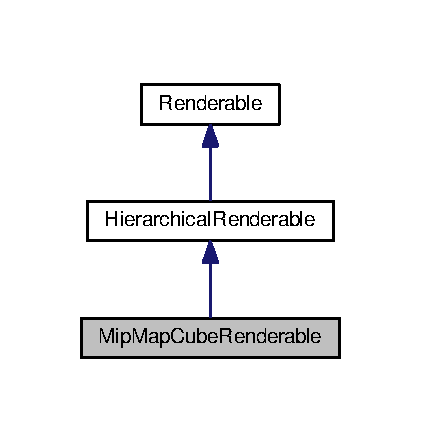
\includegraphics[width=202pt]{classMipMapCubeRenderable__inherit__graph}
\end{center}
\end{figure}


Collaboration diagram for Mip\+Map\+Cube\+Renderable\+:\nopagebreak
\begin{figure}[H]
\begin{center}
\leavevmode
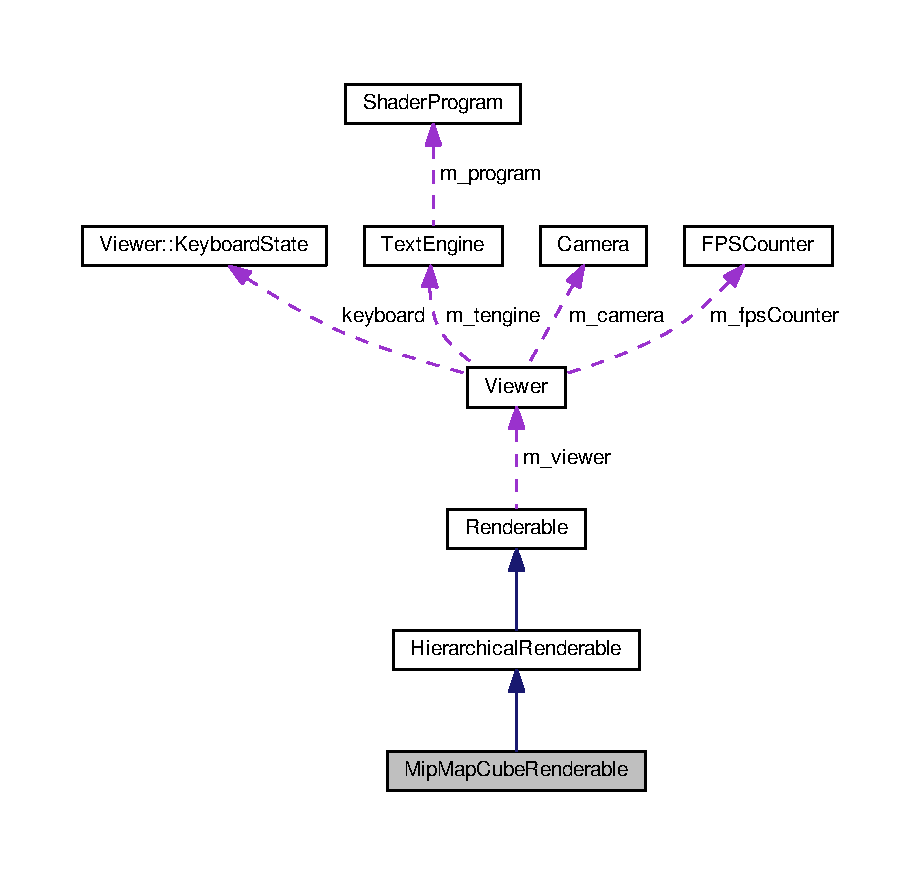
\includegraphics[width=350pt]{classMipMapCubeRenderable__coll__graph}
\end{center}
\end{figure}
\subsection*{Public Member Functions}
\begin{DoxyCompactItemize}
\item 
\hyperlink{classMipMapCubeRenderable_a891b6fb7b140fe031308f0fdb547eeb4}{$\sim$\+Mip\+Map\+Cube\+Renderable} ()
\item 
\hyperlink{classMipMapCubeRenderable_ad73277c8783cdd3e609a06a9ac3e103c}{Mip\+Map\+Cube\+Renderable} (\hyperlink{ShaderProgram_8hpp_af8e4af1ad4c53875ee5d32ab7e1f4966}{Shader\+Program\+Ptr} shader\+Program, std\+::vector$<$ std\+::string $>$ \&filenames)
\item 
void \hyperlink{classMipMapCubeRenderable_afb53a094d737952ae1053fa0eaf20812}{set\+Material} (const \hyperlink{Material_8hpp_a1d47cd05ca683e287435cf0b363fbfe1}{Material\+Ptr} \&material)
\end{DoxyCompactItemize}
\subsection*{Private Member Functions}
\begin{DoxyCompactItemize}
\item 
void \hyperlink{classMipMapCubeRenderable_a739176af783a8cb15239d86b723f9882}{do\+\_\+draw} ()
\begin{DoxyCompactList}\small\item\em Draw virtual function. \end{DoxyCompactList}\item 
void \hyperlink{classMipMapCubeRenderable_a24b35ddfe3681e641db25ed3dd46fda6}{do\+\_\+animate} (float time)
\begin{DoxyCompactList}\small\item\em Animate virtual function. \end{DoxyCompactList}\end{DoxyCompactItemize}
\subsection*{Private Attributes}
\begin{DoxyCompactItemize}
\item 
std\+::vector$<$ glm\+::vec3 $>$ \hyperlink{classMipMapCubeRenderable_a48b568e8e3cc7bf7b1f5e961b7a5d18b}{m\+\_\+positions}
\item 
std\+::vector$<$ glm\+::vec4 $>$ \hyperlink{classMipMapCubeRenderable_a5221f8391c0ef9ad9a4cc5cd0a079463}{m\+\_\+colors}
\item 
std\+::vector$<$ glm\+::vec3 $>$ \hyperlink{classMipMapCubeRenderable_adefb2e222b21ec9d5983fd578c61daa0}{m\+\_\+normals}
\item 
std\+::vector$<$ glm\+::vec2 $>$ \hyperlink{classMipMapCubeRenderable_a8c1d0d581985087fffa7328474e8167c}{m\+\_\+tex\+Coords}
\item 
unsigned int \hyperlink{classMipMapCubeRenderable_a3baff6d567731575017c9f03f28073cd}{m\+\_\+p\+Buffer}
\item 
unsigned int \hyperlink{classMipMapCubeRenderable_a1e9b398ba5e9adbfc80291d6eb64c8f3}{m\+\_\+c\+Buffer}
\item 
unsigned int \hyperlink{classMipMapCubeRenderable_a62a8adc606b023420b2089961499de09}{m\+\_\+n\+Buffer}
\item 
unsigned int \hyperlink{classMipMapCubeRenderable_a370e12a065599c98250fa40b80078a4d}{m\+\_\+t\+Buffer}
\item 
unsigned int \hyperlink{classMipMapCubeRenderable_af1dd441331717c8edffc73b18edb17e1}{m\+\_\+tex\+Id}
\item 
\hyperlink{Material_8hpp_a1d47cd05ca683e287435cf0b363fbfe1}{Material\+Ptr} \hyperlink{classMipMapCubeRenderable_a0173b7f4dbc0e7b6cc7e6ef48e05d4a1}{m\+\_\+material}
\end{DoxyCompactItemize}
\subsection*{Additional Inherited Members}


\subsection{Constructor \& Destructor Documentation}
\hypertarget{classMipMapCubeRenderable_a891b6fb7b140fe031308f0fdb547eeb4}{\index{Mip\+Map\+Cube\+Renderable@{Mip\+Map\+Cube\+Renderable}!````~Mip\+Map\+Cube\+Renderable@{$\sim$\+Mip\+Map\+Cube\+Renderable}}
\index{````~Mip\+Map\+Cube\+Renderable@{$\sim$\+Mip\+Map\+Cube\+Renderable}!Mip\+Map\+Cube\+Renderable@{Mip\+Map\+Cube\+Renderable}}
\subsubsection[{$\sim$\+Mip\+Map\+Cube\+Renderable}]{\setlength{\rightskip}{0pt plus 5cm}Mip\+Map\+Cube\+Renderable\+::$\sim$\+Mip\+Map\+Cube\+Renderable (
\begin{DoxyParamCaption}
{}
\end{DoxyParamCaption}
)}}\label{classMipMapCubeRenderable_a891b6fb7b140fe031308f0fdb547eeb4}
\hypertarget{classMipMapCubeRenderable_ad73277c8783cdd3e609a06a9ac3e103c}{\index{Mip\+Map\+Cube\+Renderable@{Mip\+Map\+Cube\+Renderable}!Mip\+Map\+Cube\+Renderable@{Mip\+Map\+Cube\+Renderable}}
\index{Mip\+Map\+Cube\+Renderable@{Mip\+Map\+Cube\+Renderable}!Mip\+Map\+Cube\+Renderable@{Mip\+Map\+Cube\+Renderable}}
\subsubsection[{Mip\+Map\+Cube\+Renderable}]{\setlength{\rightskip}{0pt plus 5cm}Mip\+Map\+Cube\+Renderable\+::\+Mip\+Map\+Cube\+Renderable (
\begin{DoxyParamCaption}
\item[{{\bf Shader\+Program\+Ptr}}]{shader\+Program, }
\item[{std\+::vector$<$ std\+::string $>$ \&}]{filenames}
\end{DoxyParamCaption}
)}}\label{classMipMapCubeRenderable_ad73277c8783cdd3e609a06a9ac3e103c}


\subsection{Member Function Documentation}
\hypertarget{classMipMapCubeRenderable_a24b35ddfe3681e641db25ed3dd46fda6}{\index{Mip\+Map\+Cube\+Renderable@{Mip\+Map\+Cube\+Renderable}!do\+\_\+animate@{do\+\_\+animate}}
\index{do\+\_\+animate@{do\+\_\+animate}!Mip\+Map\+Cube\+Renderable@{Mip\+Map\+Cube\+Renderable}}
\subsubsection[{do\+\_\+animate}]{\setlength{\rightskip}{0pt plus 5cm}void Mip\+Map\+Cube\+Renderable\+::do\+\_\+animate (
\begin{DoxyParamCaption}
\item[{float}]{time}
\end{DoxyParamCaption}
)\hspace{0.3cm}{\ttfamily [private]}, {\ttfamily [virtual]}}}\label{classMipMapCubeRenderable_a24b35ddfe3681e641db25ed3dd46fda6}
Implementation to animate this renderable. 
\begin{DoxyParams}{Parameters}
{\em time} & The current simulation time. \\
\hline
\end{DoxyParams}


Implements \hyperlink{classRenderable_aa5206322555c9dece40b21e797629b34}{Renderable}.

\hypertarget{classMipMapCubeRenderable_a739176af783a8cb15239d86b723f9882}{\index{Mip\+Map\+Cube\+Renderable@{Mip\+Map\+Cube\+Renderable}!do\+\_\+draw@{do\+\_\+draw}}
\index{do\+\_\+draw@{do\+\_\+draw}!Mip\+Map\+Cube\+Renderable@{Mip\+Map\+Cube\+Renderable}}
\subsubsection[{do\+\_\+draw}]{\setlength{\rightskip}{0pt plus 5cm}void Mip\+Map\+Cube\+Renderable\+::do\+\_\+draw (
\begin{DoxyParamCaption}
{}
\end{DoxyParamCaption}
)\hspace{0.3cm}{\ttfamily [private]}, {\ttfamily [virtual]}}}\label{classMipMapCubeRenderable_a739176af783a8cb15239d86b723f9882}
Implementation to draw this renderable. 

Implements \hyperlink{classRenderable_a98ab6308c1d2b56dacda7c435fb38d5b}{Renderable}.

\hypertarget{classMipMapCubeRenderable_afb53a094d737952ae1053fa0eaf20812}{\index{Mip\+Map\+Cube\+Renderable@{Mip\+Map\+Cube\+Renderable}!set\+Material@{set\+Material}}
\index{set\+Material@{set\+Material}!Mip\+Map\+Cube\+Renderable@{Mip\+Map\+Cube\+Renderable}}
\subsubsection[{set\+Material}]{\setlength{\rightskip}{0pt plus 5cm}void Mip\+Map\+Cube\+Renderable\+::set\+Material (
\begin{DoxyParamCaption}
\item[{const {\bf Material\+Ptr} \&}]{material}
\end{DoxyParamCaption}
)}}\label{classMipMapCubeRenderable_afb53a094d737952ae1053fa0eaf20812}


\subsection{Member Data Documentation}
\hypertarget{classMipMapCubeRenderable_a1e9b398ba5e9adbfc80291d6eb64c8f3}{\index{Mip\+Map\+Cube\+Renderable@{Mip\+Map\+Cube\+Renderable}!m\+\_\+c\+Buffer@{m\+\_\+c\+Buffer}}
\index{m\+\_\+c\+Buffer@{m\+\_\+c\+Buffer}!Mip\+Map\+Cube\+Renderable@{Mip\+Map\+Cube\+Renderable}}
\subsubsection[{m\+\_\+c\+Buffer}]{\setlength{\rightskip}{0pt plus 5cm}unsigned int Mip\+Map\+Cube\+Renderable\+::m\+\_\+c\+Buffer\hspace{0.3cm}{\ttfamily [private]}}}\label{classMipMapCubeRenderable_a1e9b398ba5e9adbfc80291d6eb64c8f3}
\hypertarget{classMipMapCubeRenderable_a5221f8391c0ef9ad9a4cc5cd0a079463}{\index{Mip\+Map\+Cube\+Renderable@{Mip\+Map\+Cube\+Renderable}!m\+\_\+colors@{m\+\_\+colors}}
\index{m\+\_\+colors@{m\+\_\+colors}!Mip\+Map\+Cube\+Renderable@{Mip\+Map\+Cube\+Renderable}}
\subsubsection[{m\+\_\+colors}]{\setlength{\rightskip}{0pt plus 5cm}std\+::vector$<$ glm\+::vec4 $>$ Mip\+Map\+Cube\+Renderable\+::m\+\_\+colors\hspace{0.3cm}{\ttfamily [private]}}}\label{classMipMapCubeRenderable_a5221f8391c0ef9ad9a4cc5cd0a079463}
\hypertarget{classMipMapCubeRenderable_a0173b7f4dbc0e7b6cc7e6ef48e05d4a1}{\index{Mip\+Map\+Cube\+Renderable@{Mip\+Map\+Cube\+Renderable}!m\+\_\+material@{m\+\_\+material}}
\index{m\+\_\+material@{m\+\_\+material}!Mip\+Map\+Cube\+Renderable@{Mip\+Map\+Cube\+Renderable}}
\subsubsection[{m\+\_\+material}]{\setlength{\rightskip}{0pt plus 5cm}{\bf Material\+Ptr} Mip\+Map\+Cube\+Renderable\+::m\+\_\+material\hspace{0.3cm}{\ttfamily [private]}}}\label{classMipMapCubeRenderable_a0173b7f4dbc0e7b6cc7e6ef48e05d4a1}
\hypertarget{classMipMapCubeRenderable_a62a8adc606b023420b2089961499de09}{\index{Mip\+Map\+Cube\+Renderable@{Mip\+Map\+Cube\+Renderable}!m\+\_\+n\+Buffer@{m\+\_\+n\+Buffer}}
\index{m\+\_\+n\+Buffer@{m\+\_\+n\+Buffer}!Mip\+Map\+Cube\+Renderable@{Mip\+Map\+Cube\+Renderable}}
\subsubsection[{m\+\_\+n\+Buffer}]{\setlength{\rightskip}{0pt plus 5cm}unsigned int Mip\+Map\+Cube\+Renderable\+::m\+\_\+n\+Buffer\hspace{0.3cm}{\ttfamily [private]}}}\label{classMipMapCubeRenderable_a62a8adc606b023420b2089961499de09}
\hypertarget{classMipMapCubeRenderable_adefb2e222b21ec9d5983fd578c61daa0}{\index{Mip\+Map\+Cube\+Renderable@{Mip\+Map\+Cube\+Renderable}!m\+\_\+normals@{m\+\_\+normals}}
\index{m\+\_\+normals@{m\+\_\+normals}!Mip\+Map\+Cube\+Renderable@{Mip\+Map\+Cube\+Renderable}}
\subsubsection[{m\+\_\+normals}]{\setlength{\rightskip}{0pt plus 5cm}std\+::vector$<$ glm\+::vec3 $>$ Mip\+Map\+Cube\+Renderable\+::m\+\_\+normals\hspace{0.3cm}{\ttfamily [private]}}}\label{classMipMapCubeRenderable_adefb2e222b21ec9d5983fd578c61daa0}
\hypertarget{classMipMapCubeRenderable_a3baff6d567731575017c9f03f28073cd}{\index{Mip\+Map\+Cube\+Renderable@{Mip\+Map\+Cube\+Renderable}!m\+\_\+p\+Buffer@{m\+\_\+p\+Buffer}}
\index{m\+\_\+p\+Buffer@{m\+\_\+p\+Buffer}!Mip\+Map\+Cube\+Renderable@{Mip\+Map\+Cube\+Renderable}}
\subsubsection[{m\+\_\+p\+Buffer}]{\setlength{\rightskip}{0pt plus 5cm}unsigned int Mip\+Map\+Cube\+Renderable\+::m\+\_\+p\+Buffer\hspace{0.3cm}{\ttfamily [private]}}}\label{classMipMapCubeRenderable_a3baff6d567731575017c9f03f28073cd}
\hypertarget{classMipMapCubeRenderable_a48b568e8e3cc7bf7b1f5e961b7a5d18b}{\index{Mip\+Map\+Cube\+Renderable@{Mip\+Map\+Cube\+Renderable}!m\+\_\+positions@{m\+\_\+positions}}
\index{m\+\_\+positions@{m\+\_\+positions}!Mip\+Map\+Cube\+Renderable@{Mip\+Map\+Cube\+Renderable}}
\subsubsection[{m\+\_\+positions}]{\setlength{\rightskip}{0pt plus 5cm}std\+::vector$<$ glm\+::vec3 $>$ Mip\+Map\+Cube\+Renderable\+::m\+\_\+positions\hspace{0.3cm}{\ttfamily [private]}}}\label{classMipMapCubeRenderable_a48b568e8e3cc7bf7b1f5e961b7a5d18b}
\hypertarget{classMipMapCubeRenderable_a370e12a065599c98250fa40b80078a4d}{\index{Mip\+Map\+Cube\+Renderable@{Mip\+Map\+Cube\+Renderable}!m\+\_\+t\+Buffer@{m\+\_\+t\+Buffer}}
\index{m\+\_\+t\+Buffer@{m\+\_\+t\+Buffer}!Mip\+Map\+Cube\+Renderable@{Mip\+Map\+Cube\+Renderable}}
\subsubsection[{m\+\_\+t\+Buffer}]{\setlength{\rightskip}{0pt plus 5cm}unsigned int Mip\+Map\+Cube\+Renderable\+::m\+\_\+t\+Buffer\hspace{0.3cm}{\ttfamily [private]}}}\label{classMipMapCubeRenderable_a370e12a065599c98250fa40b80078a4d}
\hypertarget{classMipMapCubeRenderable_a8c1d0d581985087fffa7328474e8167c}{\index{Mip\+Map\+Cube\+Renderable@{Mip\+Map\+Cube\+Renderable}!m\+\_\+tex\+Coords@{m\+\_\+tex\+Coords}}
\index{m\+\_\+tex\+Coords@{m\+\_\+tex\+Coords}!Mip\+Map\+Cube\+Renderable@{Mip\+Map\+Cube\+Renderable}}
\subsubsection[{m\+\_\+tex\+Coords}]{\setlength{\rightskip}{0pt plus 5cm}std\+::vector$<$ glm\+::vec2 $>$ Mip\+Map\+Cube\+Renderable\+::m\+\_\+tex\+Coords\hspace{0.3cm}{\ttfamily [private]}}}\label{classMipMapCubeRenderable_a8c1d0d581985087fffa7328474e8167c}
\hypertarget{classMipMapCubeRenderable_af1dd441331717c8edffc73b18edb17e1}{\index{Mip\+Map\+Cube\+Renderable@{Mip\+Map\+Cube\+Renderable}!m\+\_\+tex\+Id@{m\+\_\+tex\+Id}}
\index{m\+\_\+tex\+Id@{m\+\_\+tex\+Id}!Mip\+Map\+Cube\+Renderable@{Mip\+Map\+Cube\+Renderable}}
\subsubsection[{m\+\_\+tex\+Id}]{\setlength{\rightskip}{0pt plus 5cm}unsigned int Mip\+Map\+Cube\+Renderable\+::m\+\_\+tex\+Id\hspace{0.3cm}{\ttfamily [private]}}}\label{classMipMapCubeRenderable_af1dd441331717c8edffc73b18edb17e1}


The documentation for this class was generated from the following file\+:\begin{DoxyCompactItemize}
\item 
/home/chardon/\+Depot/ensimag/2\+A\+\_\+\+G3\+D/practicals/teacher\+Source/include/texturing/\hyperlink{MipMapCubeRenderable_8hpp}{Mip\+Map\+Cube\+Renderable.\+hpp}\end{DoxyCompactItemize}

\hypertarget{classMultiTexturedCubeRenderable}{\section{Multi\+Textured\+Cube\+Renderable Class Reference}
\label{classMultiTexturedCubeRenderable}\index{Multi\+Textured\+Cube\+Renderable@{Multi\+Textured\+Cube\+Renderable}}
}


{\ttfamily \#include $<$Multi\+Textured\+Cube\+Renderable.\+hpp$>$}



Inheritance diagram for Multi\+Textured\+Cube\+Renderable\+:\nopagebreak
\begin{figure}[H]
\begin{center}
\leavevmode
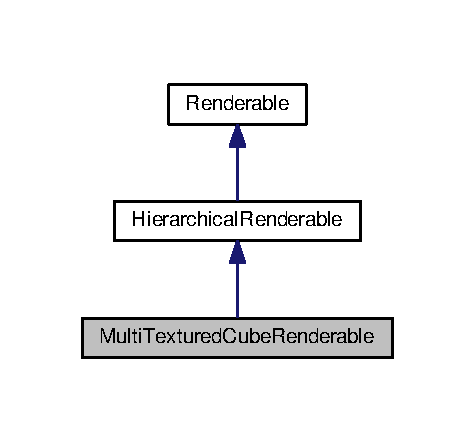
\includegraphics[width=228pt]{classMultiTexturedCubeRenderable__inherit__graph}
\end{center}
\end{figure}


Collaboration diagram for Multi\+Textured\+Cube\+Renderable\+:\nopagebreak
\begin{figure}[H]
\begin{center}
\leavevmode
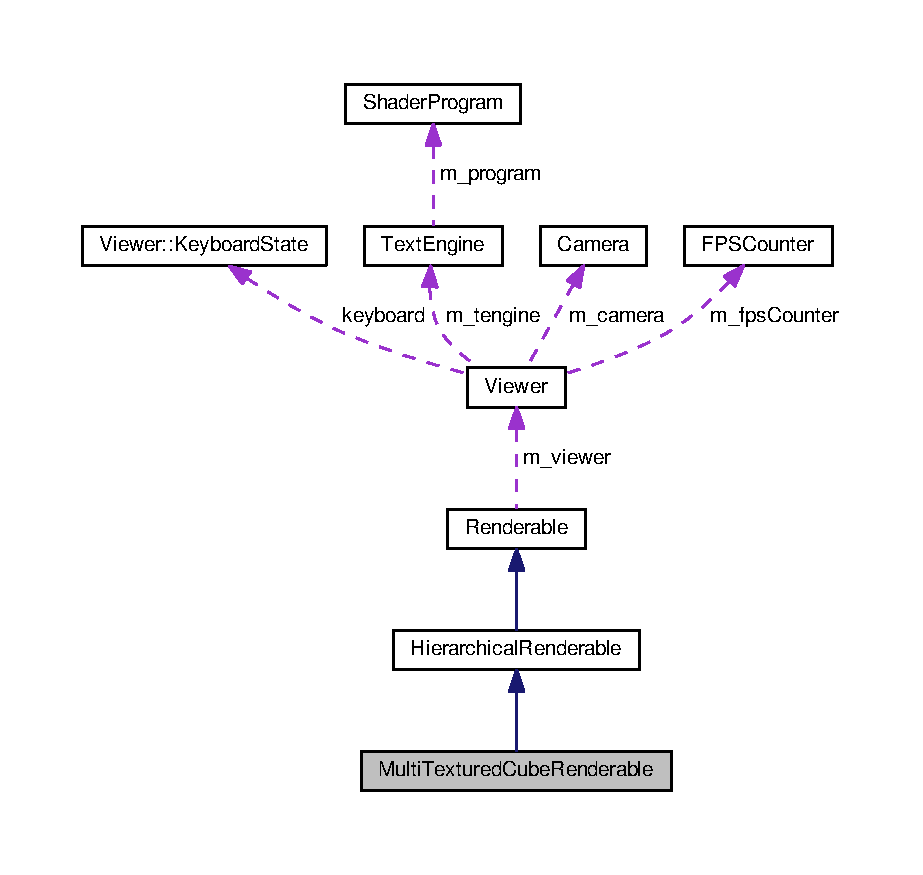
\includegraphics[width=350pt]{classMultiTexturedCubeRenderable__coll__graph}
\end{center}
\end{figure}
\subsection*{Public Member Functions}
\begin{DoxyCompactItemize}
\item 
\hyperlink{classMultiTexturedCubeRenderable_a8ded5e8d9273ed29dfbd8e07be48e883}{$\sim$\+Multi\+Textured\+Cube\+Renderable} ()
\item 
\hyperlink{classMultiTexturedCubeRenderable_a1abd417c2cbe9e71ad409e2f807bcf02}{Multi\+Textured\+Cube\+Renderable} (\hyperlink{ShaderProgram_8hpp_af8e4af1ad4c53875ee5d32ab7e1f4966}{Shader\+Program\+Ptr} shader\+Program, const std\+::string \&filename1, const std\+::string \&filename2)
\item 
void \hyperlink{classMultiTexturedCubeRenderable_a799f37e64905b22f1622d7492ebd3de0}{set\+Material} (const \hyperlink{Material_8hpp_a1d47cd05ca683e287435cf0b363fbfe1}{Material\+Ptr} \&material)
\end{DoxyCompactItemize}
\subsection*{Private Member Functions}
\begin{DoxyCompactItemize}
\item 
void \hyperlink{classMultiTexturedCubeRenderable_a3dafc49b8a8b6b5f9ed2928c91c2cd6f}{do\+\_\+draw} ()
\begin{DoxyCompactList}\small\item\em Draw virtual function. \end{DoxyCompactList}\item 
void \hyperlink{classMultiTexturedCubeRenderable_a1db1e5f6c10f62874aef22e346906979}{do\+\_\+animate} (float time)
\begin{DoxyCompactList}\small\item\em Animate virtual function. \end{DoxyCompactList}\end{DoxyCompactItemize}
\subsection*{Private Attributes}
\begin{DoxyCompactItemize}
\item 
std\+::vector$<$ glm\+::vec3 $>$ \hyperlink{classMultiTexturedCubeRenderable_a60daa9382a5a20272fe5aff5f06c7fac}{m\+\_\+positions}
\item 
std\+::vector$<$ glm\+::vec4 $>$ \hyperlink{classMultiTexturedCubeRenderable_a6b898288adb8ab29e4faf8557094d81d}{m\+\_\+colors}
\item 
std\+::vector$<$ glm\+::vec3 $>$ \hyperlink{classMultiTexturedCubeRenderable_a240496a75e60b0ed5af4dfafad198fa7}{m\+\_\+normals}
\item 
std\+::vector$<$ glm\+::vec2 $>$ \hyperlink{classMultiTexturedCubeRenderable_a527036e4aa13864829e20a897a16f8cf}{m\+\_\+tex\+Coords1}
\item 
std\+::vector$<$ glm\+::vec2 $>$ \hyperlink{classMultiTexturedCubeRenderable_adcab47d5610c8f989658103a3cd2e8c8}{m\+\_\+tex\+Coords2}
\item 
unsigned int \hyperlink{classMultiTexturedCubeRenderable_aa9e62d83d66f405662bf3e92be2564ea}{m\+\_\+p\+Buffer}
\item 
unsigned int \hyperlink{classMultiTexturedCubeRenderable_af11d0075bbe8aa521fae8fb437ff98af}{m\+\_\+c\+Buffer}
\item 
unsigned int \hyperlink{classMultiTexturedCubeRenderable_a49898f71f097b8e6ffe3383a019f3d5c}{m\+\_\+n\+Buffer}
\item 
unsigned int \hyperlink{classMultiTexturedCubeRenderable_a789fa5e3d95bb43f2fe209ddf0a68884}{m\+\_\+t\+Buffer1}
\item 
unsigned int \hyperlink{classMultiTexturedCubeRenderable_ae541f09397856a5bde7c1db6962ebe54}{m\+\_\+t\+Buffer2}
\item 
unsigned int \hyperlink{classMultiTexturedCubeRenderable_ac00c241a06009cd3650bc09658209394}{m\+\_\+tex\+Id1}
\item 
unsigned int \hyperlink{classMultiTexturedCubeRenderable_a84eb4a8f43e2eed94101b563c61aae0c}{m\+\_\+tex\+Id2}
\item 
float \hyperlink{classMultiTexturedCubeRenderable_a91914ee0e86d087d1778d1ecd461256f}{m\+\_\+blending\+Coefficient}
\item 
\hyperlink{Material_8hpp_a1d47cd05ca683e287435cf0b363fbfe1}{Material\+Ptr} \hyperlink{classMultiTexturedCubeRenderable_a7fa7b1dce63798c5f3a319e6fb6f2859}{m\+\_\+material}
\end{DoxyCompactItemize}
\subsection*{Additional Inherited Members}


\subsection{Constructor \& Destructor Documentation}
\hypertarget{classMultiTexturedCubeRenderable_a8ded5e8d9273ed29dfbd8e07be48e883}{\index{Multi\+Textured\+Cube\+Renderable@{Multi\+Textured\+Cube\+Renderable}!````~Multi\+Textured\+Cube\+Renderable@{$\sim$\+Multi\+Textured\+Cube\+Renderable}}
\index{````~Multi\+Textured\+Cube\+Renderable@{$\sim$\+Multi\+Textured\+Cube\+Renderable}!Multi\+Textured\+Cube\+Renderable@{Multi\+Textured\+Cube\+Renderable}}
\subsubsection[{$\sim$\+Multi\+Textured\+Cube\+Renderable}]{\setlength{\rightskip}{0pt plus 5cm}Multi\+Textured\+Cube\+Renderable\+::$\sim$\+Multi\+Textured\+Cube\+Renderable (
\begin{DoxyParamCaption}
{}
\end{DoxyParamCaption}
)}}\label{classMultiTexturedCubeRenderable_a8ded5e8d9273ed29dfbd8e07be48e883}
\hypertarget{classMultiTexturedCubeRenderable_a1abd417c2cbe9e71ad409e2f807bcf02}{\index{Multi\+Textured\+Cube\+Renderable@{Multi\+Textured\+Cube\+Renderable}!Multi\+Textured\+Cube\+Renderable@{Multi\+Textured\+Cube\+Renderable}}
\index{Multi\+Textured\+Cube\+Renderable@{Multi\+Textured\+Cube\+Renderable}!Multi\+Textured\+Cube\+Renderable@{Multi\+Textured\+Cube\+Renderable}}
\subsubsection[{Multi\+Textured\+Cube\+Renderable}]{\setlength{\rightskip}{0pt plus 5cm}Multi\+Textured\+Cube\+Renderable\+::\+Multi\+Textured\+Cube\+Renderable (
\begin{DoxyParamCaption}
\item[{{\bf Shader\+Program\+Ptr}}]{shader\+Program, }
\item[{const std\+::string \&}]{filename1, }
\item[{const std\+::string \&}]{filename2}
\end{DoxyParamCaption}
)}}\label{classMultiTexturedCubeRenderable_a1abd417c2cbe9e71ad409e2f807bcf02}


\subsection{Member Function Documentation}
\hypertarget{classMultiTexturedCubeRenderable_a1db1e5f6c10f62874aef22e346906979}{\index{Multi\+Textured\+Cube\+Renderable@{Multi\+Textured\+Cube\+Renderable}!do\+\_\+animate@{do\+\_\+animate}}
\index{do\+\_\+animate@{do\+\_\+animate}!Multi\+Textured\+Cube\+Renderable@{Multi\+Textured\+Cube\+Renderable}}
\subsubsection[{do\+\_\+animate}]{\setlength{\rightskip}{0pt plus 5cm}void Multi\+Textured\+Cube\+Renderable\+::do\+\_\+animate (
\begin{DoxyParamCaption}
\item[{float}]{time}
\end{DoxyParamCaption}
)\hspace{0.3cm}{\ttfamily [private]}, {\ttfamily [virtual]}}}\label{classMultiTexturedCubeRenderable_a1db1e5f6c10f62874aef22e346906979}
Implementation to animate this renderable. 
\begin{DoxyParams}{Parameters}
{\em time} & The current simulation time. \\
\hline
\end{DoxyParams}


Implements \hyperlink{classRenderable_aa5206322555c9dece40b21e797629b34}{Renderable}.

\hypertarget{classMultiTexturedCubeRenderable_a3dafc49b8a8b6b5f9ed2928c91c2cd6f}{\index{Multi\+Textured\+Cube\+Renderable@{Multi\+Textured\+Cube\+Renderable}!do\+\_\+draw@{do\+\_\+draw}}
\index{do\+\_\+draw@{do\+\_\+draw}!Multi\+Textured\+Cube\+Renderable@{Multi\+Textured\+Cube\+Renderable}}
\subsubsection[{do\+\_\+draw}]{\setlength{\rightskip}{0pt plus 5cm}void Multi\+Textured\+Cube\+Renderable\+::do\+\_\+draw (
\begin{DoxyParamCaption}
{}
\end{DoxyParamCaption}
)\hspace{0.3cm}{\ttfamily [private]}, {\ttfamily [virtual]}}}\label{classMultiTexturedCubeRenderable_a3dafc49b8a8b6b5f9ed2928c91c2cd6f}
Implementation to draw this renderable. 

Implements \hyperlink{classRenderable_a98ab6308c1d2b56dacda7c435fb38d5b}{Renderable}.

\hypertarget{classMultiTexturedCubeRenderable_a799f37e64905b22f1622d7492ebd3de0}{\index{Multi\+Textured\+Cube\+Renderable@{Multi\+Textured\+Cube\+Renderable}!set\+Material@{set\+Material}}
\index{set\+Material@{set\+Material}!Multi\+Textured\+Cube\+Renderable@{Multi\+Textured\+Cube\+Renderable}}
\subsubsection[{set\+Material}]{\setlength{\rightskip}{0pt plus 5cm}void Multi\+Textured\+Cube\+Renderable\+::set\+Material (
\begin{DoxyParamCaption}
\item[{const {\bf Material\+Ptr} \&}]{material}
\end{DoxyParamCaption}
)}}\label{classMultiTexturedCubeRenderable_a799f37e64905b22f1622d7492ebd3de0}


\subsection{Member Data Documentation}
\hypertarget{classMultiTexturedCubeRenderable_a91914ee0e86d087d1778d1ecd461256f}{\index{Multi\+Textured\+Cube\+Renderable@{Multi\+Textured\+Cube\+Renderable}!m\+\_\+blending\+Coefficient@{m\+\_\+blending\+Coefficient}}
\index{m\+\_\+blending\+Coefficient@{m\+\_\+blending\+Coefficient}!Multi\+Textured\+Cube\+Renderable@{Multi\+Textured\+Cube\+Renderable}}
\subsubsection[{m\+\_\+blending\+Coefficient}]{\setlength{\rightskip}{0pt plus 5cm}float Multi\+Textured\+Cube\+Renderable\+::m\+\_\+blending\+Coefficient\hspace{0.3cm}{\ttfamily [private]}}}\label{classMultiTexturedCubeRenderable_a91914ee0e86d087d1778d1ecd461256f}
\hypertarget{classMultiTexturedCubeRenderable_af11d0075bbe8aa521fae8fb437ff98af}{\index{Multi\+Textured\+Cube\+Renderable@{Multi\+Textured\+Cube\+Renderable}!m\+\_\+c\+Buffer@{m\+\_\+c\+Buffer}}
\index{m\+\_\+c\+Buffer@{m\+\_\+c\+Buffer}!Multi\+Textured\+Cube\+Renderable@{Multi\+Textured\+Cube\+Renderable}}
\subsubsection[{m\+\_\+c\+Buffer}]{\setlength{\rightskip}{0pt plus 5cm}unsigned int Multi\+Textured\+Cube\+Renderable\+::m\+\_\+c\+Buffer\hspace{0.3cm}{\ttfamily [private]}}}\label{classMultiTexturedCubeRenderable_af11d0075bbe8aa521fae8fb437ff98af}
\hypertarget{classMultiTexturedCubeRenderable_a6b898288adb8ab29e4faf8557094d81d}{\index{Multi\+Textured\+Cube\+Renderable@{Multi\+Textured\+Cube\+Renderable}!m\+\_\+colors@{m\+\_\+colors}}
\index{m\+\_\+colors@{m\+\_\+colors}!Multi\+Textured\+Cube\+Renderable@{Multi\+Textured\+Cube\+Renderable}}
\subsubsection[{m\+\_\+colors}]{\setlength{\rightskip}{0pt plus 5cm}std\+::vector$<$ glm\+::vec4 $>$ Multi\+Textured\+Cube\+Renderable\+::m\+\_\+colors\hspace{0.3cm}{\ttfamily [private]}}}\label{classMultiTexturedCubeRenderable_a6b898288adb8ab29e4faf8557094d81d}
\hypertarget{classMultiTexturedCubeRenderable_a7fa7b1dce63798c5f3a319e6fb6f2859}{\index{Multi\+Textured\+Cube\+Renderable@{Multi\+Textured\+Cube\+Renderable}!m\+\_\+material@{m\+\_\+material}}
\index{m\+\_\+material@{m\+\_\+material}!Multi\+Textured\+Cube\+Renderable@{Multi\+Textured\+Cube\+Renderable}}
\subsubsection[{m\+\_\+material}]{\setlength{\rightskip}{0pt plus 5cm}{\bf Material\+Ptr} Multi\+Textured\+Cube\+Renderable\+::m\+\_\+material\hspace{0.3cm}{\ttfamily [private]}}}\label{classMultiTexturedCubeRenderable_a7fa7b1dce63798c5f3a319e6fb6f2859}
\hypertarget{classMultiTexturedCubeRenderable_a49898f71f097b8e6ffe3383a019f3d5c}{\index{Multi\+Textured\+Cube\+Renderable@{Multi\+Textured\+Cube\+Renderable}!m\+\_\+n\+Buffer@{m\+\_\+n\+Buffer}}
\index{m\+\_\+n\+Buffer@{m\+\_\+n\+Buffer}!Multi\+Textured\+Cube\+Renderable@{Multi\+Textured\+Cube\+Renderable}}
\subsubsection[{m\+\_\+n\+Buffer}]{\setlength{\rightskip}{0pt plus 5cm}unsigned int Multi\+Textured\+Cube\+Renderable\+::m\+\_\+n\+Buffer\hspace{0.3cm}{\ttfamily [private]}}}\label{classMultiTexturedCubeRenderable_a49898f71f097b8e6ffe3383a019f3d5c}
\hypertarget{classMultiTexturedCubeRenderable_a240496a75e60b0ed5af4dfafad198fa7}{\index{Multi\+Textured\+Cube\+Renderable@{Multi\+Textured\+Cube\+Renderable}!m\+\_\+normals@{m\+\_\+normals}}
\index{m\+\_\+normals@{m\+\_\+normals}!Multi\+Textured\+Cube\+Renderable@{Multi\+Textured\+Cube\+Renderable}}
\subsubsection[{m\+\_\+normals}]{\setlength{\rightskip}{0pt plus 5cm}std\+::vector$<$ glm\+::vec3 $>$ Multi\+Textured\+Cube\+Renderable\+::m\+\_\+normals\hspace{0.3cm}{\ttfamily [private]}}}\label{classMultiTexturedCubeRenderable_a240496a75e60b0ed5af4dfafad198fa7}
\hypertarget{classMultiTexturedCubeRenderable_aa9e62d83d66f405662bf3e92be2564ea}{\index{Multi\+Textured\+Cube\+Renderable@{Multi\+Textured\+Cube\+Renderable}!m\+\_\+p\+Buffer@{m\+\_\+p\+Buffer}}
\index{m\+\_\+p\+Buffer@{m\+\_\+p\+Buffer}!Multi\+Textured\+Cube\+Renderable@{Multi\+Textured\+Cube\+Renderable}}
\subsubsection[{m\+\_\+p\+Buffer}]{\setlength{\rightskip}{0pt plus 5cm}unsigned int Multi\+Textured\+Cube\+Renderable\+::m\+\_\+p\+Buffer\hspace{0.3cm}{\ttfamily [private]}}}\label{classMultiTexturedCubeRenderable_aa9e62d83d66f405662bf3e92be2564ea}
\hypertarget{classMultiTexturedCubeRenderable_a60daa9382a5a20272fe5aff5f06c7fac}{\index{Multi\+Textured\+Cube\+Renderable@{Multi\+Textured\+Cube\+Renderable}!m\+\_\+positions@{m\+\_\+positions}}
\index{m\+\_\+positions@{m\+\_\+positions}!Multi\+Textured\+Cube\+Renderable@{Multi\+Textured\+Cube\+Renderable}}
\subsubsection[{m\+\_\+positions}]{\setlength{\rightskip}{0pt plus 5cm}std\+::vector$<$ glm\+::vec3 $>$ Multi\+Textured\+Cube\+Renderable\+::m\+\_\+positions\hspace{0.3cm}{\ttfamily [private]}}}\label{classMultiTexturedCubeRenderable_a60daa9382a5a20272fe5aff5f06c7fac}
\hypertarget{classMultiTexturedCubeRenderable_a789fa5e3d95bb43f2fe209ddf0a68884}{\index{Multi\+Textured\+Cube\+Renderable@{Multi\+Textured\+Cube\+Renderable}!m\+\_\+t\+Buffer1@{m\+\_\+t\+Buffer1}}
\index{m\+\_\+t\+Buffer1@{m\+\_\+t\+Buffer1}!Multi\+Textured\+Cube\+Renderable@{Multi\+Textured\+Cube\+Renderable}}
\subsubsection[{m\+\_\+t\+Buffer1}]{\setlength{\rightskip}{0pt plus 5cm}unsigned int Multi\+Textured\+Cube\+Renderable\+::m\+\_\+t\+Buffer1\hspace{0.3cm}{\ttfamily [private]}}}\label{classMultiTexturedCubeRenderable_a789fa5e3d95bb43f2fe209ddf0a68884}
\hypertarget{classMultiTexturedCubeRenderable_ae541f09397856a5bde7c1db6962ebe54}{\index{Multi\+Textured\+Cube\+Renderable@{Multi\+Textured\+Cube\+Renderable}!m\+\_\+t\+Buffer2@{m\+\_\+t\+Buffer2}}
\index{m\+\_\+t\+Buffer2@{m\+\_\+t\+Buffer2}!Multi\+Textured\+Cube\+Renderable@{Multi\+Textured\+Cube\+Renderable}}
\subsubsection[{m\+\_\+t\+Buffer2}]{\setlength{\rightskip}{0pt plus 5cm}unsigned int Multi\+Textured\+Cube\+Renderable\+::m\+\_\+t\+Buffer2\hspace{0.3cm}{\ttfamily [private]}}}\label{classMultiTexturedCubeRenderable_ae541f09397856a5bde7c1db6962ebe54}
\hypertarget{classMultiTexturedCubeRenderable_a527036e4aa13864829e20a897a16f8cf}{\index{Multi\+Textured\+Cube\+Renderable@{Multi\+Textured\+Cube\+Renderable}!m\+\_\+tex\+Coords1@{m\+\_\+tex\+Coords1}}
\index{m\+\_\+tex\+Coords1@{m\+\_\+tex\+Coords1}!Multi\+Textured\+Cube\+Renderable@{Multi\+Textured\+Cube\+Renderable}}
\subsubsection[{m\+\_\+tex\+Coords1}]{\setlength{\rightskip}{0pt plus 5cm}std\+::vector$<$ glm\+::vec2$>$ Multi\+Textured\+Cube\+Renderable\+::m\+\_\+tex\+Coords1\hspace{0.3cm}{\ttfamily [private]}}}\label{classMultiTexturedCubeRenderable_a527036e4aa13864829e20a897a16f8cf}
\hypertarget{classMultiTexturedCubeRenderable_adcab47d5610c8f989658103a3cd2e8c8}{\index{Multi\+Textured\+Cube\+Renderable@{Multi\+Textured\+Cube\+Renderable}!m\+\_\+tex\+Coords2@{m\+\_\+tex\+Coords2}}
\index{m\+\_\+tex\+Coords2@{m\+\_\+tex\+Coords2}!Multi\+Textured\+Cube\+Renderable@{Multi\+Textured\+Cube\+Renderable}}
\subsubsection[{m\+\_\+tex\+Coords2}]{\setlength{\rightskip}{0pt plus 5cm}std\+::vector$<$ glm\+::vec2$>$ Multi\+Textured\+Cube\+Renderable\+::m\+\_\+tex\+Coords2\hspace{0.3cm}{\ttfamily [private]}}}\label{classMultiTexturedCubeRenderable_adcab47d5610c8f989658103a3cd2e8c8}
\hypertarget{classMultiTexturedCubeRenderable_ac00c241a06009cd3650bc09658209394}{\index{Multi\+Textured\+Cube\+Renderable@{Multi\+Textured\+Cube\+Renderable}!m\+\_\+tex\+Id1@{m\+\_\+tex\+Id1}}
\index{m\+\_\+tex\+Id1@{m\+\_\+tex\+Id1}!Multi\+Textured\+Cube\+Renderable@{Multi\+Textured\+Cube\+Renderable}}
\subsubsection[{m\+\_\+tex\+Id1}]{\setlength{\rightskip}{0pt plus 5cm}unsigned int Multi\+Textured\+Cube\+Renderable\+::m\+\_\+tex\+Id1\hspace{0.3cm}{\ttfamily [private]}}}\label{classMultiTexturedCubeRenderable_ac00c241a06009cd3650bc09658209394}
\hypertarget{classMultiTexturedCubeRenderable_a84eb4a8f43e2eed94101b563c61aae0c}{\index{Multi\+Textured\+Cube\+Renderable@{Multi\+Textured\+Cube\+Renderable}!m\+\_\+tex\+Id2@{m\+\_\+tex\+Id2}}
\index{m\+\_\+tex\+Id2@{m\+\_\+tex\+Id2}!Multi\+Textured\+Cube\+Renderable@{Multi\+Textured\+Cube\+Renderable}}
\subsubsection[{m\+\_\+tex\+Id2}]{\setlength{\rightskip}{0pt plus 5cm}unsigned int Multi\+Textured\+Cube\+Renderable\+::m\+\_\+tex\+Id2\hspace{0.3cm}{\ttfamily [private]}}}\label{classMultiTexturedCubeRenderable_a84eb4a8f43e2eed94101b563c61aae0c}


The documentation for this class was generated from the following file\+:\begin{DoxyCompactItemize}
\item 
/home/chardon/\+Depot/ensimag/2\+A\+\_\+\+G3\+D/practicals/teacher\+Source/include/texturing/\hyperlink{MultiTexturedCubeRenderable_8hpp}{Multi\+Textured\+Cube\+Renderable.\+hpp}\end{DoxyCompactItemize}

\hypertarget{classParticle}{\section{Particle Class Reference}
\label{classParticle}\index{Particle@{Particle}}
}


Represent a particle as a moving ball.  




{\ttfamily \#include $<$Particle.\+hpp$>$}

\subsection*{Public Member Functions}
\begin{DoxyCompactItemize}
\item 
\hyperlink{classParticle_a8e0174413f7c34f67ca992552e409ced}{Particle} (const glm\+::vec3 \&position, const glm\+::vec3 \&velocity, const float \&mass, const float \&radius)
\begin{DoxyCompactList}\small\item\em Instantiate a dynamic particle. \end{DoxyCompactList}\item 
\hyperlink{classParticle_ad030d0fe7b88cf81744b127c99244ff4}{$\sim$\+Particle} ()
\item 
const glm\+::vec3 \& \hyperlink{classParticle_a40b65e9c27b1265ac48ce4925e37f619}{get\+Position} () const 
\begin{DoxyCompactList}\small\item\em Access to this particle's position. \end{DoxyCompactList}\item 
const glm\+::vec3 \& \hyperlink{classParticle_af976b4aa95a792454c75d2143e0bf5cf}{get\+Velocity} () const 
\begin{DoxyCompactList}\small\item\em Access to this particle's velocity. \end{DoxyCompactList}\item 
const glm\+::vec3 \& \hyperlink{classParticle_a9bde826461065bc609e7a859cca54b8d}{get\+Force} () const 
\begin{DoxyCompactList}\small\item\em Access to this particle's applied force. \end{DoxyCompactList}\item 
float \hyperlink{classParticle_af11c8e6d590e50496d637b3822e4fdaa}{get\+Mass} () const 
\begin{DoxyCompactList}\small\item\em Access to this particle's mass. \end{DoxyCompactList}\item 
float \hyperlink{classParticle_a34b87163953d21f8ba23f960a7927e52}{get\+Radius} () const 
\begin{DoxyCompactList}\small\item\em Access to this particle's radius. \end{DoxyCompactList}\item 
bool \hyperlink{classParticle_a9d41e6acd3b52ff439b3a4903f630fcd}{is\+Fixed} () const 
\begin{DoxyCompactList}\small\item\em Check if this particle is fixed. \end{DoxyCompactList}\item 
void \hyperlink{classParticle_aee41362c732ae8a7cca20d872e5a3fc1}{set\+Position} (const glm\+::vec3 \&pos)
\begin{DoxyCompactList}\small\item\em Set the particle's position. \end{DoxyCompactList}\item 
void \hyperlink{classParticle_acbab01a9093288cdd1242b24e5de80a9}{set\+Velocity} (const glm\+::vec3 \&vel)
\begin{DoxyCompactList}\small\item\em Set the particle's velocity. \end{DoxyCompactList}\item 
void \hyperlink{classParticle_af07a51b823e3570623e2b6fcd43d01df}{set\+Force} (const glm\+::vec3 \&force)
\begin{DoxyCompactList}\small\item\em Set the particle's applied force. \end{DoxyCompactList}\item 
void \hyperlink{classParticle_a03c5c0de979488aa04f2541637945eea}{set\+Radius} (const float \&radius)
\begin{DoxyCompactList}\small\item\em Set the particle's radius. \end{DoxyCompactList}\item 
void \hyperlink{classParticle_a81e84b1b27570a749bd92a309dc12f25}{set\+Fixed} (bool \hyperlink{classParticle_a9d41e6acd3b52ff439b3a4903f630fcd}{is\+Fixed})
\begin{DoxyCompactList}\small\item\em Set the particle's fixed flag. \end{DoxyCompactList}\item 
void \hyperlink{classParticle_aaa74f8dfdb197454efb785f59393719c}{incr\+Position} (const glm\+::vec3 \&pos)
\begin{DoxyCompactList}\small\item\em Increment the particle's position. \end{DoxyCompactList}\item 
void \hyperlink{classParticle_a281ec390b081eedb09324b82bf2051f9}{incr\+Velocity} (const glm\+::vec3 \&vel)
\begin{DoxyCompactList}\small\item\em Increment the particle's velocity. \end{DoxyCompactList}\item 
void \hyperlink{classParticle_ac78ce769340d2362374f29f5805cc796}{incr\+Force} (const glm\+::vec3 \&force)
\begin{DoxyCompactList}\small\item\em Increment the particle's applied force. \end{DoxyCompactList}\item 
void \hyperlink{classParticle_aa850ffa01940b79df28fb1cd9f68bf45}{restart} ()
\begin{DoxyCompactList}\small\item\em Restart the particle. \end{DoxyCompactList}\end{DoxyCompactItemize}
\subsection*{Private Attributes}
\begin{DoxyCompactItemize}
\item 
const glm\+::vec3 \hyperlink{classParticle_aa6c61c14e6ef274fb54700a5912e78bf}{m\+\_\+initial\+Position}
\begin{DoxyCompactList}\small\item\em The initial particle's position. \end{DoxyCompactList}\item 
const glm\+::vec3 \hyperlink{classParticle_af83d2d60768349ca902f83de1a59e355}{m\+\_\+initial\+Velocity}
\begin{DoxyCompactList}\small\item\em The initial particle's velocity. \end{DoxyCompactList}\item 
glm\+::vec3 \hyperlink{classParticle_ad6daec7ed061255747fbe26ee88429c6}{m\+\_\+position}
\begin{DoxyCompactList}\small\item\em The particle's position. \end{DoxyCompactList}\item 
glm\+::vec3 \hyperlink{classParticle_ae8433e1a1968203478096f319a04e111}{m\+\_\+velocity}
\begin{DoxyCompactList}\small\item\em The particle's velocity. \end{DoxyCompactList}\item 
glm\+::vec3 \hyperlink{classParticle_af4db2db523aa91152dab38bc2ed1e460}{m\+\_\+force}
\begin{DoxyCompactList}\small\item\em The particle's applied force. \end{DoxyCompactList}\item 
float \hyperlink{classParticle_ab78b76aeb4d163132a0c27ea4c5beb75}{m\+\_\+mass}
\begin{DoxyCompactList}\small\item\em The particle's mass. \end{DoxyCompactList}\item 
float \hyperlink{classParticle_af6aee0d324572f74a1bdc28937d04a0b}{m\+\_\+radius}
\begin{DoxyCompactList}\small\item\em The particle's radius. \end{DoxyCompactList}\item 
bool \hyperlink{classParticle_a1a986129338efef4273582fd5ce9eaac}{m\+\_\+is\+Fixed}
\begin{DoxyCompactList}\small\item\em The particle's fixed flag. \end{DoxyCompactList}\end{DoxyCompactItemize}


\subsection{Detailed Description}
This class is used to model particles in a dynamic system. Such a particle is seen as a ball with a mass, a velocity and a position. This ball is affected by forces that will change both its position and its velocity. This ball can be fixed, making its position constant and its velocity null. 

\subsection{Constructor \& Destructor Documentation}
\hypertarget{classParticle_a8e0174413f7c34f67ca992552e409ced}{\index{Particle@{Particle}!Particle@{Particle}}
\index{Particle@{Particle}!Particle@{Particle}}
\subsubsection[{Particle}]{\setlength{\rightskip}{0pt plus 5cm}Particle\+::\+Particle (
\begin{DoxyParamCaption}
\item[{const glm\+::vec3 \&}]{position, }
\item[{const glm\+::vec3 \&}]{velocity, }
\item[{const float \&}]{mass, }
\item[{const float \&}]{radius}
\end{DoxyParamCaption}
)}}\label{classParticle_a8e0174413f7c34f67ca992552e409ced}
Construct a new particle, represented as a moving ball. The initial position and velocity are saved in order to be restored when the simulation restarts.


\begin{DoxyParams}{Parameters}
{\em position} & The initial position. \\
\hline
{\em velocity} & The initial speed. \\
\hline
{\em mass} & The particle mass. \\
\hline
{\em radius} & The particle radius. \\
\hline
\end{DoxyParams}
\hypertarget{classParticle_ad030d0fe7b88cf81744b127c99244ff4}{\index{Particle@{Particle}!````~Particle@{$\sim$\+Particle}}
\index{````~Particle@{$\sim$\+Particle}!Particle@{Particle}}
\subsubsection[{$\sim$\+Particle}]{\setlength{\rightskip}{0pt plus 5cm}Particle\+::$\sim$\+Particle (
\begin{DoxyParamCaption}
{}
\end{DoxyParamCaption}
)}}\label{classParticle_ad030d0fe7b88cf81744b127c99244ff4}


\subsection{Member Function Documentation}
\hypertarget{classParticle_a9bde826461065bc609e7a859cca54b8d}{\index{Particle@{Particle}!get\+Force@{get\+Force}}
\index{get\+Force@{get\+Force}!Particle@{Particle}}
\subsubsection[{get\+Force}]{\setlength{\rightskip}{0pt plus 5cm}const glm\+::vec3\& Particle\+::get\+Force (
\begin{DoxyParamCaption}
{}
\end{DoxyParamCaption}
) const}}\label{classParticle_a9bde826461065bc609e7a859cca54b8d}
Get the force applied to this particle. \begin{DoxyReturn}{Returns}
The particle's applied force. 
\end{DoxyReturn}
\hypertarget{classParticle_af11c8e6d590e50496d637b3822e4fdaa}{\index{Particle@{Particle}!get\+Mass@{get\+Mass}}
\index{get\+Mass@{get\+Mass}!Particle@{Particle}}
\subsubsection[{get\+Mass}]{\setlength{\rightskip}{0pt plus 5cm}float Particle\+::get\+Mass (
\begin{DoxyParamCaption}
{}
\end{DoxyParamCaption}
) const}}\label{classParticle_af11c8e6d590e50496d637b3822e4fdaa}
Get the mass of this particle. \begin{DoxyReturn}{Returns}
The particle's mass. 
\end{DoxyReturn}
\hypertarget{classParticle_a40b65e9c27b1265ac48ce4925e37f619}{\index{Particle@{Particle}!get\+Position@{get\+Position}}
\index{get\+Position@{get\+Position}!Particle@{Particle}}
\subsubsection[{get\+Position}]{\setlength{\rightskip}{0pt plus 5cm}const glm\+::vec3\& Particle\+::get\+Position (
\begin{DoxyParamCaption}
{}
\end{DoxyParamCaption}
) const}}\label{classParticle_a40b65e9c27b1265ac48ce4925e37f619}
Get the position of this particle. \begin{DoxyReturn}{Returns}
The particle's position. 
\end{DoxyReturn}
\hypertarget{classParticle_a34b87163953d21f8ba23f960a7927e52}{\index{Particle@{Particle}!get\+Radius@{get\+Radius}}
\index{get\+Radius@{get\+Radius}!Particle@{Particle}}
\subsubsection[{get\+Radius}]{\setlength{\rightskip}{0pt plus 5cm}float Particle\+::get\+Radius (
\begin{DoxyParamCaption}
{}
\end{DoxyParamCaption}
) const}}\label{classParticle_a34b87163953d21f8ba23f960a7927e52}
Get the radius of this particle. \begin{DoxyReturn}{Returns}
The particle's radius. 
\end{DoxyReturn}
\hypertarget{classParticle_af976b4aa95a792454c75d2143e0bf5cf}{\index{Particle@{Particle}!get\+Velocity@{get\+Velocity}}
\index{get\+Velocity@{get\+Velocity}!Particle@{Particle}}
\subsubsection[{get\+Velocity}]{\setlength{\rightskip}{0pt plus 5cm}const glm\+::vec3\& Particle\+::get\+Velocity (
\begin{DoxyParamCaption}
{}
\end{DoxyParamCaption}
) const}}\label{classParticle_af976b4aa95a792454c75d2143e0bf5cf}
Get the velocity of this particle. \begin{DoxyReturn}{Returns}
The particle's velocity. 
\end{DoxyReturn}
\hypertarget{classParticle_ac78ce769340d2362374f29f5805cc796}{\index{Particle@{Particle}!incr\+Force@{incr\+Force}}
\index{incr\+Force@{incr\+Force}!Particle@{Particle}}
\subsubsection[{incr\+Force}]{\setlength{\rightskip}{0pt plus 5cm}void Particle\+::incr\+Force (
\begin{DoxyParamCaption}
\item[{const glm\+::vec3 \&}]{force}
\end{DoxyParamCaption}
)}}\label{classParticle_ac78ce769340d2362374f29f5805cc796}
Increment the force applied to this particle. 
\begin{DoxyParams}{Parameters}
{\em force} & The force to add to this particle's applied force, i.\+e. m\+\_\+force += force. \\
\hline
\end{DoxyParams}
\hypertarget{classParticle_aaa74f8dfdb197454efb785f59393719c}{\index{Particle@{Particle}!incr\+Position@{incr\+Position}}
\index{incr\+Position@{incr\+Position}!Particle@{Particle}}
\subsubsection[{incr\+Position}]{\setlength{\rightskip}{0pt plus 5cm}void Particle\+::incr\+Position (
\begin{DoxyParamCaption}
\item[{const glm\+::vec3 \&}]{pos}
\end{DoxyParamCaption}
)}}\label{classParticle_aaa74f8dfdb197454efb785f59393719c}
Increment the position of this particle. 
\begin{DoxyParams}{Parameters}
{\em pos} & The position to add to this particle's position, i.\+e. m\+\_\+position += pos. \\
\hline
\end{DoxyParams}
\hypertarget{classParticle_a281ec390b081eedb09324b82bf2051f9}{\index{Particle@{Particle}!incr\+Velocity@{incr\+Velocity}}
\index{incr\+Velocity@{incr\+Velocity}!Particle@{Particle}}
\subsubsection[{incr\+Velocity}]{\setlength{\rightskip}{0pt plus 5cm}void Particle\+::incr\+Velocity (
\begin{DoxyParamCaption}
\item[{const glm\+::vec3 \&}]{vel}
\end{DoxyParamCaption}
)}}\label{classParticle_a281ec390b081eedb09324b82bf2051f9}
Increment the velocity of this particle. 
\begin{DoxyParams}{Parameters}
{\em vel} & The velocity to add to this particle's velocity, i.\+e. m\+\_\+velocity += vel. \\
\hline
\end{DoxyParams}
\hypertarget{classParticle_a9d41e6acd3b52ff439b3a4903f630fcd}{\index{Particle@{Particle}!is\+Fixed@{is\+Fixed}}
\index{is\+Fixed@{is\+Fixed}!Particle@{Particle}}
\subsubsection[{is\+Fixed}]{\setlength{\rightskip}{0pt plus 5cm}bool Particle\+::is\+Fixed (
\begin{DoxyParamCaption}
{}
\end{DoxyParamCaption}
) const}}\label{classParticle_a9d41e6acd3b52ff439b3a4903f630fcd}
Check if this particle is fixed. \begin{DoxyReturn}{Returns}
True if the particle is fixed. 
\end{DoxyReturn}
\hypertarget{classParticle_aa850ffa01940b79df28fb1cd9f68bf45}{\index{Particle@{Particle}!restart@{restart}}
\index{restart@{restart}!Particle@{Particle}}
\subsubsection[{restart}]{\setlength{\rightskip}{0pt plus 5cm}void Particle\+::restart (
\begin{DoxyParamCaption}
{}
\end{DoxyParamCaption}
)}}\label{classParticle_aa850ffa01940b79df28fb1cd9f68bf45}
Set the particle's position and velocity to their initial values. \hypertarget{classParticle_a81e84b1b27570a749bd92a309dc12f25}{\index{Particle@{Particle}!set\+Fixed@{set\+Fixed}}
\index{set\+Fixed@{set\+Fixed}!Particle@{Particle}}
\subsubsection[{set\+Fixed}]{\setlength{\rightskip}{0pt plus 5cm}void Particle\+::set\+Fixed (
\begin{DoxyParamCaption}
\item[{bool}]{is\+Fixed}
\end{DoxyParamCaption}
)}}\label{classParticle_a81e84b1b27570a749bd92a309dc12f25}
Set the fixed flag of this particle. 
\begin{DoxyParams}{Parameters}
{\em is\+Fixed} & The new value of the fixed flag. \\
\hline
\end{DoxyParams}
\hypertarget{classParticle_af07a51b823e3570623e2b6fcd43d01df}{\index{Particle@{Particle}!set\+Force@{set\+Force}}
\index{set\+Force@{set\+Force}!Particle@{Particle}}
\subsubsection[{set\+Force}]{\setlength{\rightskip}{0pt plus 5cm}void Particle\+::set\+Force (
\begin{DoxyParamCaption}
\item[{const glm\+::vec3 \&}]{force}
\end{DoxyParamCaption}
)}}\label{classParticle_af07a51b823e3570623e2b6fcd43d01df}
Set the force applied to this particle. 
\begin{DoxyParams}{Parameters}
{\em force} & The new force applied to this particle. \\
\hline
\end{DoxyParams}
\hypertarget{classParticle_aee41362c732ae8a7cca20d872e5a3fc1}{\index{Particle@{Particle}!set\+Position@{set\+Position}}
\index{set\+Position@{set\+Position}!Particle@{Particle}}
\subsubsection[{set\+Position}]{\setlength{\rightskip}{0pt plus 5cm}void Particle\+::set\+Position (
\begin{DoxyParamCaption}
\item[{const glm\+::vec3 \&}]{pos}
\end{DoxyParamCaption}
)}}\label{classParticle_aee41362c732ae8a7cca20d872e5a3fc1}
Set the position of this particle. 
\begin{DoxyParams}{Parameters}
{\em pos} & The new position of this particle. \\
\hline
\end{DoxyParams}
\hypertarget{classParticle_a03c5c0de979488aa04f2541637945eea}{\index{Particle@{Particle}!set\+Radius@{set\+Radius}}
\index{set\+Radius@{set\+Radius}!Particle@{Particle}}
\subsubsection[{set\+Radius}]{\setlength{\rightskip}{0pt plus 5cm}void Particle\+::set\+Radius (
\begin{DoxyParamCaption}
\item[{const float \&}]{radius}
\end{DoxyParamCaption}
)}}\label{classParticle_a03c5c0de979488aa04f2541637945eea}
Set the radius of this particle. 
\begin{DoxyParams}{Parameters}
{\em radius} & The new radius of this particle. \\
\hline
\end{DoxyParams}
\hypertarget{classParticle_acbab01a9093288cdd1242b24e5de80a9}{\index{Particle@{Particle}!set\+Velocity@{set\+Velocity}}
\index{set\+Velocity@{set\+Velocity}!Particle@{Particle}}
\subsubsection[{set\+Velocity}]{\setlength{\rightskip}{0pt plus 5cm}void Particle\+::set\+Velocity (
\begin{DoxyParamCaption}
\item[{const glm\+::vec3 \&}]{vel}
\end{DoxyParamCaption}
)}}\label{classParticle_acbab01a9093288cdd1242b24e5de80a9}
Set the velocity of this particle. 
\begin{DoxyParams}{Parameters}
{\em vel} & The new velocity of this particle. \\
\hline
\end{DoxyParams}


\subsection{Member Data Documentation}
\hypertarget{classParticle_af4db2db523aa91152dab38bc2ed1e460}{\index{Particle@{Particle}!m\+\_\+force@{m\+\_\+force}}
\index{m\+\_\+force@{m\+\_\+force}!Particle@{Particle}}
\subsubsection[{m\+\_\+force}]{\setlength{\rightskip}{0pt plus 5cm}glm\+::vec3 Particle\+::m\+\_\+force\hspace{0.3cm}{\ttfamily [private]}}}\label{classParticle_af4db2db523aa91152dab38bc2ed1e460}
The force applied to this particle. \hypertarget{classParticle_aa6c61c14e6ef274fb54700a5912e78bf}{\index{Particle@{Particle}!m\+\_\+initial\+Position@{m\+\_\+initial\+Position}}
\index{m\+\_\+initial\+Position@{m\+\_\+initial\+Position}!Particle@{Particle}}
\subsubsection[{m\+\_\+initial\+Position}]{\setlength{\rightskip}{0pt plus 5cm}const glm\+::vec3 Particle\+::m\+\_\+initial\+Position\hspace{0.3cm}{\ttfamily [private]}}}\label{classParticle_aa6c61c14e6ef274fb54700a5912e78bf}
The initial position of this particle, stored to be set at restart. \hypertarget{classParticle_af83d2d60768349ca902f83de1a59e355}{\index{Particle@{Particle}!m\+\_\+initial\+Velocity@{m\+\_\+initial\+Velocity}}
\index{m\+\_\+initial\+Velocity@{m\+\_\+initial\+Velocity}!Particle@{Particle}}
\subsubsection[{m\+\_\+initial\+Velocity}]{\setlength{\rightskip}{0pt plus 5cm}const glm\+::vec3 Particle\+::m\+\_\+initial\+Velocity\hspace{0.3cm}{\ttfamily [private]}}}\label{classParticle_af83d2d60768349ca902f83de1a59e355}
The initial velocity of this particle, stored to be set at restart. \hypertarget{classParticle_a1a986129338efef4273582fd5ce9eaac}{\index{Particle@{Particle}!m\+\_\+is\+Fixed@{m\+\_\+is\+Fixed}}
\index{m\+\_\+is\+Fixed@{m\+\_\+is\+Fixed}!Particle@{Particle}}
\subsubsection[{m\+\_\+is\+Fixed}]{\setlength{\rightskip}{0pt plus 5cm}bool Particle\+::m\+\_\+is\+Fixed\hspace{0.3cm}{\ttfamily [private]}}}\label{classParticle_a1a986129338efef4273582fd5ce9eaac}
A flag that tells if this particle is fixed. If set to true, the position should be constant and the velocity null in simulation steps. \hypertarget{classParticle_ab78b76aeb4d163132a0c27ea4c5beb75}{\index{Particle@{Particle}!m\+\_\+mass@{m\+\_\+mass}}
\index{m\+\_\+mass@{m\+\_\+mass}!Particle@{Particle}}
\subsubsection[{m\+\_\+mass}]{\setlength{\rightskip}{0pt plus 5cm}float Particle\+::m\+\_\+mass\hspace{0.3cm}{\ttfamily [private]}}}\label{classParticle_ab78b76aeb4d163132a0c27ea4c5beb75}
The mass of this particle. \hypertarget{classParticle_ad6daec7ed061255747fbe26ee88429c6}{\index{Particle@{Particle}!m\+\_\+position@{m\+\_\+position}}
\index{m\+\_\+position@{m\+\_\+position}!Particle@{Particle}}
\subsubsection[{m\+\_\+position}]{\setlength{\rightskip}{0pt plus 5cm}glm\+::vec3 Particle\+::m\+\_\+position\hspace{0.3cm}{\ttfamily [private]}}}\label{classParticle_ad6daec7ed061255747fbe26ee88429c6}
The position of this particle. \hypertarget{classParticle_af6aee0d324572f74a1bdc28937d04a0b}{\index{Particle@{Particle}!m\+\_\+radius@{m\+\_\+radius}}
\index{m\+\_\+radius@{m\+\_\+radius}!Particle@{Particle}}
\subsubsection[{m\+\_\+radius}]{\setlength{\rightskip}{0pt plus 5cm}float Particle\+::m\+\_\+radius\hspace{0.3cm}{\ttfamily [private]}}}\label{classParticle_af6aee0d324572f74a1bdc28937d04a0b}
The radius of this particle. \hypertarget{classParticle_ae8433e1a1968203478096f319a04e111}{\index{Particle@{Particle}!m\+\_\+velocity@{m\+\_\+velocity}}
\index{m\+\_\+velocity@{m\+\_\+velocity}!Particle@{Particle}}
\subsubsection[{m\+\_\+velocity}]{\setlength{\rightskip}{0pt plus 5cm}glm\+::vec3 Particle\+::m\+\_\+velocity\hspace{0.3cm}{\ttfamily [private]}}}\label{classParticle_ae8433e1a1968203478096f319a04e111}
The position of this particle. 

The documentation for this class was generated from the following file\+:\begin{DoxyCompactItemize}
\item 
/home/chardon/\+Depot/ensimag/2\+A\+\_\+\+G3\+D/practicals/teacher\+Source/include/dynamics/\hyperlink{Particle_8hpp}{Particle.\+hpp}\end{DoxyCompactItemize}

\hypertarget{classParticleListRenderable}{\section{Particle\+List\+Renderable Class Reference}
\label{classParticleListRenderable}\index{Particle\+List\+Renderable@{Particle\+List\+Renderable}}
}


Draw a list of particles.  




{\ttfamily \#include $<$Particle\+List\+Renderable.\+hpp$>$}



Inheritance diagram for Particle\+List\+Renderable\+:\nopagebreak
\begin{figure}[H]
\begin{center}
\leavevmode
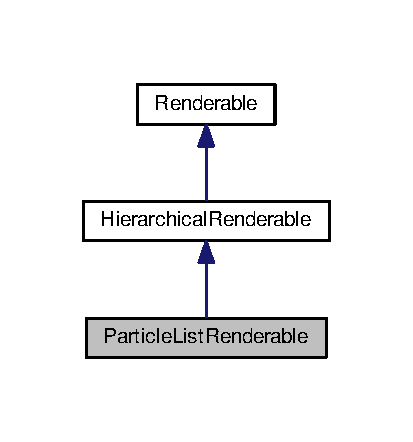
\includegraphics[width=198pt]{classParticleListRenderable__inherit__graph}
\end{center}
\end{figure}


Collaboration diagram for Particle\+List\+Renderable\+:\nopagebreak
\begin{figure}[H]
\begin{center}
\leavevmode
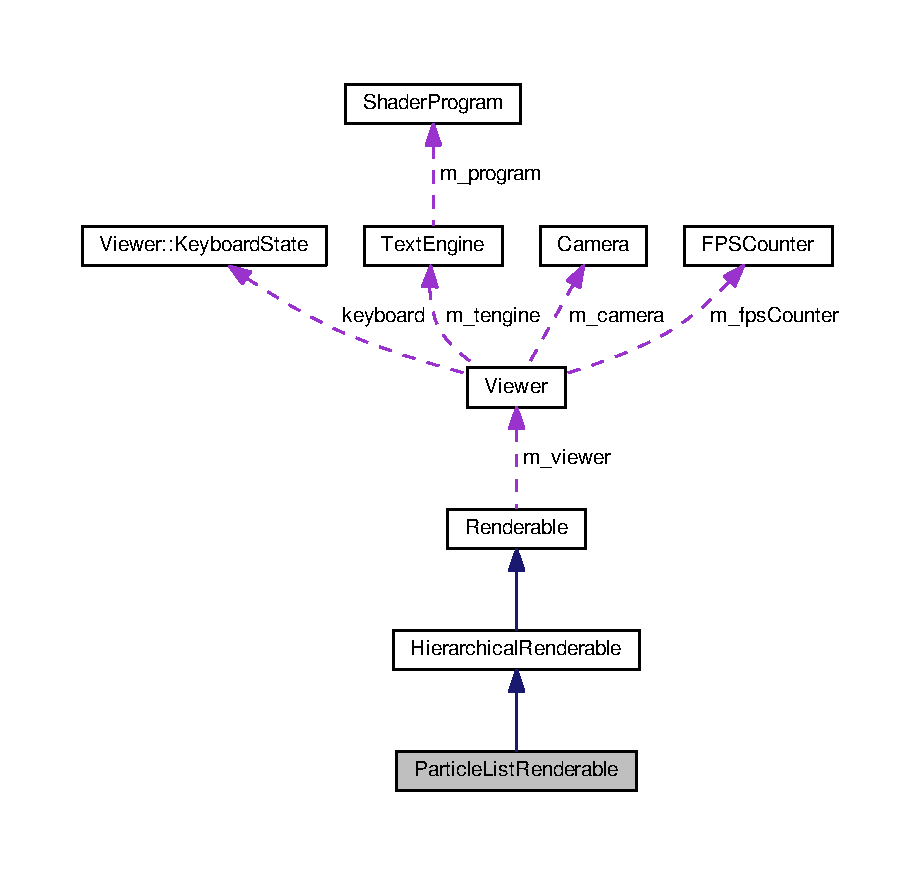
\includegraphics[width=350pt]{classParticleListRenderable__coll__graph}
\end{center}
\end{figure}
\subsection*{Public Member Functions}
\begin{DoxyCompactItemize}
\item 
\hyperlink{classParticleListRenderable_a24b513eaf7e3c847270d7da34cb1208d}{$\sim$\+Particle\+List\+Renderable} ()
\item 
\hyperlink{classParticleListRenderable_a847158b58dccb013af2902b40361363e}{Particle\+List\+Renderable} (\hyperlink{ShaderProgram_8hpp_af8e4af1ad4c53875ee5d32ab7e1f4966}{Shader\+Program\+Ptr} program, std\+::vector$<$ \hyperlink{Particle_8hpp_a9a7abc8635002993537b61ef2c857fdd}{Particle\+Ptr} $>$ \&particles)
\begin{DoxyCompactList}\small\item\em Build a renderable to render a set of particles. \end{DoxyCompactList}\end{DoxyCompactItemize}
\subsection*{Private Member Functions}
\begin{DoxyCompactItemize}
\item 
void \hyperlink{classParticleListRenderable_af34f9d0c377aa749e52d226d9cf49d89}{do\+\_\+draw} ()
\begin{DoxyCompactList}\small\item\em Draw virtual function. \end{DoxyCompactList}\item 
void \hyperlink{classParticleListRenderable_a25adb6020cb86abb50d33d76a5cde1f1}{do\+\_\+animate} (float time)
\begin{DoxyCompactList}\small\item\em Animate virtual function. \end{DoxyCompactList}\end{DoxyCompactItemize}
\subsection*{Private Attributes}
\begin{DoxyCompactItemize}
\item 
std\+::vector$<$ \hyperlink{Particle_8hpp_a9a7abc8635002993537b61ef2c857fdd}{Particle\+Ptr} $>$ \hyperlink{classParticleListRenderable_a2debf6d432dfd9854718e0c16c4f6f51}{m\+\_\+particles}
\item 
size\+\_\+t \hyperlink{classParticleListRenderable_a0971e99dfa53c5729d040b6a96d47a4f}{m\+\_\+number\+Of\+Vertices}
\item 
unsigned int \hyperlink{classParticleListRenderable_a87f491d5861bb1b9f98541e5926c4c5e}{m\+\_\+position\+Buffer}
\item 
unsigned int \hyperlink{classParticleListRenderable_a7e967af4fe279662d35d1cf08e4e2e86}{m\+\_\+color\+Buffer}
\item 
unsigned int \hyperlink{classParticleListRenderable_ae6b22324c801f946afe8a9eee5ff7be5}{m\+\_\+normal\+Buffer}
\end{DoxyCompactItemize}
\subsection*{Additional Inherited Members}


\subsection{Detailed Description}
This class is used to draw a list of particle. This is more efficient than to render individually each particle. We could do even more efficient but it is beyond the objectives of those practicals. 

\subsection{Constructor \& Destructor Documentation}
\hypertarget{classParticleListRenderable_a24b513eaf7e3c847270d7da34cb1208d}{\index{Particle\+List\+Renderable@{Particle\+List\+Renderable}!````~Particle\+List\+Renderable@{$\sim$\+Particle\+List\+Renderable}}
\index{````~Particle\+List\+Renderable@{$\sim$\+Particle\+List\+Renderable}!Particle\+List\+Renderable@{Particle\+List\+Renderable}}
\subsubsection[{$\sim$\+Particle\+List\+Renderable}]{\setlength{\rightskip}{0pt plus 5cm}Particle\+List\+Renderable\+::$\sim$\+Particle\+List\+Renderable (
\begin{DoxyParamCaption}
{}
\end{DoxyParamCaption}
)}}\label{classParticleListRenderable_a24b513eaf7e3c847270d7da34cb1208d}
\hypertarget{classParticleListRenderable_a847158b58dccb013af2902b40361363e}{\index{Particle\+List\+Renderable@{Particle\+List\+Renderable}!Particle\+List\+Renderable@{Particle\+List\+Renderable}}
\index{Particle\+List\+Renderable@{Particle\+List\+Renderable}!Particle\+List\+Renderable@{Particle\+List\+Renderable}}
\subsubsection[{Particle\+List\+Renderable}]{\setlength{\rightskip}{0pt plus 5cm}Particle\+List\+Renderable\+::\+Particle\+List\+Renderable (
\begin{DoxyParamCaption}
\item[{{\bf Shader\+Program\+Ptr}}]{program, }
\item[{std\+::vector$<$ {\bf Particle\+Ptr} $>$ \&}]{particles}
\end{DoxyParamCaption}
)}}\label{classParticleListRenderable_a847158b58dccb013af2902b40361363e}
Build a renderable to render a set of particles. 
\begin{DoxyParams}{Parameters}
{\em program} & The shader program used to render the particles. \\
\hline
{\em particles} & The set of particles to render. \\
\hline
\end{DoxyParams}


\subsection{Member Function Documentation}
\hypertarget{classParticleListRenderable_a25adb6020cb86abb50d33d76a5cde1f1}{\index{Particle\+List\+Renderable@{Particle\+List\+Renderable}!do\+\_\+animate@{do\+\_\+animate}}
\index{do\+\_\+animate@{do\+\_\+animate}!Particle\+List\+Renderable@{Particle\+List\+Renderable}}
\subsubsection[{do\+\_\+animate}]{\setlength{\rightskip}{0pt plus 5cm}void Particle\+List\+Renderable\+::do\+\_\+animate (
\begin{DoxyParamCaption}
\item[{float}]{time}
\end{DoxyParamCaption}
)\hspace{0.3cm}{\ttfamily [private]}, {\ttfamily [virtual]}}}\label{classParticleListRenderable_a25adb6020cb86abb50d33d76a5cde1f1}
Implementation to animate this renderable. 
\begin{DoxyParams}{Parameters}
{\em time} & The current simulation time. \\
\hline
\end{DoxyParams}


Implements \hyperlink{classRenderable_aa5206322555c9dece40b21e797629b34}{Renderable}.

\hypertarget{classParticleListRenderable_af34f9d0c377aa749e52d226d9cf49d89}{\index{Particle\+List\+Renderable@{Particle\+List\+Renderable}!do\+\_\+draw@{do\+\_\+draw}}
\index{do\+\_\+draw@{do\+\_\+draw}!Particle\+List\+Renderable@{Particle\+List\+Renderable}}
\subsubsection[{do\+\_\+draw}]{\setlength{\rightskip}{0pt plus 5cm}void Particle\+List\+Renderable\+::do\+\_\+draw (
\begin{DoxyParamCaption}
{}
\end{DoxyParamCaption}
)\hspace{0.3cm}{\ttfamily [private]}, {\ttfamily [virtual]}}}\label{classParticleListRenderable_af34f9d0c377aa749e52d226d9cf49d89}
Implementation to draw this renderable. 

Implements \hyperlink{classRenderable_a98ab6308c1d2b56dacda7c435fb38d5b}{Renderable}.



\subsection{Member Data Documentation}
\hypertarget{classParticleListRenderable_a7e967af4fe279662d35d1cf08e4e2e86}{\index{Particle\+List\+Renderable@{Particle\+List\+Renderable}!m\+\_\+color\+Buffer@{m\+\_\+color\+Buffer}}
\index{m\+\_\+color\+Buffer@{m\+\_\+color\+Buffer}!Particle\+List\+Renderable@{Particle\+List\+Renderable}}
\subsubsection[{m\+\_\+color\+Buffer}]{\setlength{\rightskip}{0pt plus 5cm}unsigned int Particle\+List\+Renderable\+::m\+\_\+color\+Buffer\hspace{0.3cm}{\ttfamily [private]}}}\label{classParticleListRenderable_a7e967af4fe279662d35d1cf08e4e2e86}
\hypertarget{classParticleListRenderable_ae6b22324c801f946afe8a9eee5ff7be5}{\index{Particle\+List\+Renderable@{Particle\+List\+Renderable}!m\+\_\+normal\+Buffer@{m\+\_\+normal\+Buffer}}
\index{m\+\_\+normal\+Buffer@{m\+\_\+normal\+Buffer}!Particle\+List\+Renderable@{Particle\+List\+Renderable}}
\subsubsection[{m\+\_\+normal\+Buffer}]{\setlength{\rightskip}{0pt plus 5cm}unsigned int Particle\+List\+Renderable\+::m\+\_\+normal\+Buffer\hspace{0.3cm}{\ttfamily [private]}}}\label{classParticleListRenderable_ae6b22324c801f946afe8a9eee5ff7be5}
\hypertarget{classParticleListRenderable_a0971e99dfa53c5729d040b6a96d47a4f}{\index{Particle\+List\+Renderable@{Particle\+List\+Renderable}!m\+\_\+number\+Of\+Vertices@{m\+\_\+number\+Of\+Vertices}}
\index{m\+\_\+number\+Of\+Vertices@{m\+\_\+number\+Of\+Vertices}!Particle\+List\+Renderable@{Particle\+List\+Renderable}}
\subsubsection[{m\+\_\+number\+Of\+Vertices}]{\setlength{\rightskip}{0pt plus 5cm}size\+\_\+t Particle\+List\+Renderable\+::m\+\_\+number\+Of\+Vertices\hspace{0.3cm}{\ttfamily [private]}}}\label{classParticleListRenderable_a0971e99dfa53c5729d040b6a96d47a4f}
\hypertarget{classParticleListRenderable_a2debf6d432dfd9854718e0c16c4f6f51}{\index{Particle\+List\+Renderable@{Particle\+List\+Renderable}!m\+\_\+particles@{m\+\_\+particles}}
\index{m\+\_\+particles@{m\+\_\+particles}!Particle\+List\+Renderable@{Particle\+List\+Renderable}}
\subsubsection[{m\+\_\+particles}]{\setlength{\rightskip}{0pt plus 5cm}std\+::vector$<$ {\bf Particle\+Ptr} $>$ Particle\+List\+Renderable\+::m\+\_\+particles\hspace{0.3cm}{\ttfamily [private]}}}\label{classParticleListRenderable_a2debf6d432dfd9854718e0c16c4f6f51}
\hypertarget{classParticleListRenderable_a87f491d5861bb1b9f98541e5926c4c5e}{\index{Particle\+List\+Renderable@{Particle\+List\+Renderable}!m\+\_\+position\+Buffer@{m\+\_\+position\+Buffer}}
\index{m\+\_\+position\+Buffer@{m\+\_\+position\+Buffer}!Particle\+List\+Renderable@{Particle\+List\+Renderable}}
\subsubsection[{m\+\_\+position\+Buffer}]{\setlength{\rightskip}{0pt plus 5cm}unsigned int Particle\+List\+Renderable\+::m\+\_\+position\+Buffer\hspace{0.3cm}{\ttfamily [private]}}}\label{classParticleListRenderable_a87f491d5861bb1b9f98541e5926c4c5e}


The documentation for this class was generated from the following file\+:\begin{DoxyCompactItemize}
\item 
/home/chardon/\+Depot/ensimag/2\+A\+\_\+\+G3\+D/practicals/teacher\+Source/include/dynamics/\hyperlink{ParticleListRenderable_8hpp}{Particle\+List\+Renderable.\+hpp}\end{DoxyCompactItemize}

\hypertarget{classParticleParticleCollision}{\section{Particle\+Particle\+Collision Class Reference}
\label{classParticleParticleCollision}\index{Particle\+Particle\+Collision@{Particle\+Particle\+Collision}}
}


Implement the resolution of a collision event between two particles.  




{\ttfamily \#include $<$Particle\+Particle\+Collision.\+hpp$>$}



Inheritance diagram for Particle\+Particle\+Collision\+:\nopagebreak
\begin{figure}[H]
\begin{center}
\leavevmode
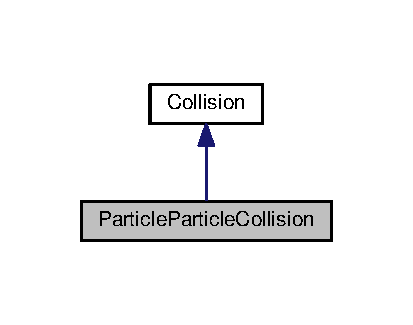
\includegraphics[width=198pt]{classParticleParticleCollision__inherit__graph}
\end{center}
\end{figure}


Collaboration diagram for Particle\+Particle\+Collision\+:\nopagebreak
\begin{figure}[H]
\begin{center}
\leavevmode
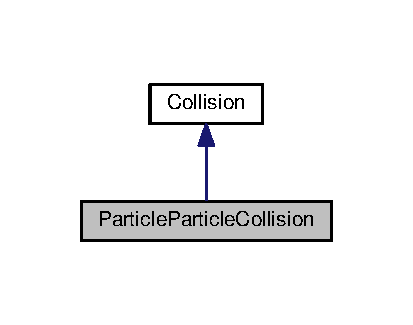
\includegraphics[width=198pt]{classParticleParticleCollision__coll__graph}
\end{center}
\end{figure}
\subsection*{Public Member Functions}
\begin{DoxyCompactItemize}
\item 
\hyperlink{classParticleParticleCollision_acec460f38329b2347f044ac295f5c47c}{$\sim$\+Particle\+Particle\+Collision} ()
\item 
\hyperlink{classParticleParticleCollision_aef8e68092353ac4843c7cd4626dd60fc}{Particle\+Particle\+Collision} (\hyperlink{Particle_8hpp_a9a7abc8635002993537b61ef2c857fdd}{Particle\+Ptr} particle1, \hyperlink{Particle_8hpp_a9a7abc8635002993537b61ef2c857fdd}{Particle\+Ptr} particle2, float restitution)
\begin{DoxyCompactList}\small\item\em Build a new collision event between two particles. \end{DoxyCompactList}\end{DoxyCompactItemize}
\subsection*{Private Member Functions}
\begin{DoxyCompactItemize}
\item 
void \hyperlink{classParticleParticleCollision_a9f18947965d8615faf1d957c259a65e2}{do\+\_\+solve\+Collision} ()
\begin{DoxyCompactList}\small\item\em Implementation of the collision solving. \end{DoxyCompactList}\end{DoxyCompactItemize}
\subsection*{Private Attributes}
\begin{DoxyCompactItemize}
\item 
\hyperlink{Particle_8hpp_a9a7abc8635002993537b61ef2c857fdd}{Particle\+Ptr} \hyperlink{classParticleParticleCollision_a6ed4f0ca756feef481b59ba27c6f260c}{m\+\_\+p1}
\item 
\hyperlink{Particle_8hpp_a9a7abc8635002993537b61ef2c857fdd}{Particle\+Ptr} \hyperlink{classParticleParticleCollision_a31615486eff94310643ce85e3e40d539}{m\+\_\+p2}
\end{DoxyCompactItemize}
\subsection*{Additional Inherited Members}


\subsection{Detailed Description}
Implementation of the resolution of a collision between two particles. 

\subsection{Constructor \& Destructor Documentation}
\hypertarget{classParticleParticleCollision_acec460f38329b2347f044ac295f5c47c}{\index{Particle\+Particle\+Collision@{Particle\+Particle\+Collision}!````~Particle\+Particle\+Collision@{$\sim$\+Particle\+Particle\+Collision}}
\index{````~Particle\+Particle\+Collision@{$\sim$\+Particle\+Particle\+Collision}!Particle\+Particle\+Collision@{Particle\+Particle\+Collision}}
\subsubsection[{$\sim$\+Particle\+Particle\+Collision}]{\setlength{\rightskip}{0pt plus 5cm}Particle\+Particle\+Collision\+::$\sim$\+Particle\+Particle\+Collision (
\begin{DoxyParamCaption}
{}
\end{DoxyParamCaption}
)}}\label{classParticleParticleCollision_acec460f38329b2347f044ac295f5c47c}
\hypertarget{classParticleParticleCollision_aef8e68092353ac4843c7cd4626dd60fc}{\index{Particle\+Particle\+Collision@{Particle\+Particle\+Collision}!Particle\+Particle\+Collision@{Particle\+Particle\+Collision}}
\index{Particle\+Particle\+Collision@{Particle\+Particle\+Collision}!Particle\+Particle\+Collision@{Particle\+Particle\+Collision}}
\subsubsection[{Particle\+Particle\+Collision}]{\setlength{\rightskip}{0pt plus 5cm}Particle\+Particle\+Collision\+::\+Particle\+Particle\+Collision (
\begin{DoxyParamCaption}
\item[{{\bf Particle\+Ptr}}]{particle1, }
\item[{{\bf Particle\+Ptr}}]{particle2, }
\item[{float}]{restitution}
\end{DoxyParamCaption}
)}}\label{classParticleParticleCollision_aef8e68092353ac4843c7cd4626dd60fc}
Build a collision event between two particles. 
\begin{DoxyParams}{Parameters}
{\em particle1} & The first colliding particle. \\
\hline
{\em particle2} & The second colliding particle. \\
\hline
{\em restitution} & The restitution factor of the collision. \\
\hline
\end{DoxyParams}


\subsection{Member Function Documentation}
\hypertarget{classParticleParticleCollision_a9f18947965d8615faf1d957c259a65e2}{\index{Particle\+Particle\+Collision@{Particle\+Particle\+Collision}!do\+\_\+solve\+Collision@{do\+\_\+solve\+Collision}}
\index{do\+\_\+solve\+Collision@{do\+\_\+solve\+Collision}!Particle\+Particle\+Collision@{Particle\+Particle\+Collision}}
\subsubsection[{do\+\_\+solve\+Collision}]{\setlength{\rightskip}{0pt plus 5cm}void Particle\+Particle\+Collision\+::do\+\_\+solve\+Collision (
\begin{DoxyParamCaption}
{}
\end{DoxyParamCaption}
)\hspace{0.3cm}{\ttfamily [private]}, {\ttfamily [virtual]}}}\label{classParticleParticleCollision_a9f18947965d8615faf1d957c259a65e2}
Actual implementation of the collision solving, that should be done in derived classes. 

Implements \hyperlink{classCollision_a5fa2b29df51abd8723660cd07050e616}{Collision}.



\subsection{Member Data Documentation}
\hypertarget{classParticleParticleCollision_a6ed4f0ca756feef481b59ba27c6f260c}{\index{Particle\+Particle\+Collision@{Particle\+Particle\+Collision}!m\+\_\+p1@{m\+\_\+p1}}
\index{m\+\_\+p1@{m\+\_\+p1}!Particle\+Particle\+Collision@{Particle\+Particle\+Collision}}
\subsubsection[{m\+\_\+p1}]{\setlength{\rightskip}{0pt plus 5cm}{\bf Particle\+Ptr} Particle\+Particle\+Collision\+::m\+\_\+p1\hspace{0.3cm}{\ttfamily [private]}}}\label{classParticleParticleCollision_a6ed4f0ca756feef481b59ba27c6f260c}
\hypertarget{classParticleParticleCollision_a31615486eff94310643ce85e3e40d539}{\index{Particle\+Particle\+Collision@{Particle\+Particle\+Collision}!m\+\_\+p2@{m\+\_\+p2}}
\index{m\+\_\+p2@{m\+\_\+p2}!Particle\+Particle\+Collision@{Particle\+Particle\+Collision}}
\subsubsection[{m\+\_\+p2}]{\setlength{\rightskip}{0pt plus 5cm}{\bf Particle\+Ptr} Particle\+Particle\+Collision\+::m\+\_\+p2\hspace{0.3cm}{\ttfamily [private]}}}\label{classParticleParticleCollision_a31615486eff94310643ce85e3e40d539}


The documentation for this class was generated from the following file\+:\begin{DoxyCompactItemize}
\item 
/home/chardon/\+Depot/ensimag/2\+A\+\_\+\+G3\+D/practicals/teacher\+Source/include/dynamics/\hyperlink{ParticleParticleCollision_8hpp}{Particle\+Particle\+Collision.\+hpp}\end{DoxyCompactItemize}

\hypertarget{classParticlePlaneCollision}{\section{Particle\+Plane\+Collision Class Reference}
\label{classParticlePlaneCollision}\index{Particle\+Plane\+Collision@{Particle\+Plane\+Collision}}
}


Implement the resolution of a collision event between a plane and a particle.  




{\ttfamily \#include $<$Particle\+Plane\+Collision.\+hpp$>$}



Inheritance diagram for Particle\+Plane\+Collision\+:\nopagebreak
\begin{figure}[H]
\begin{center}
\leavevmode
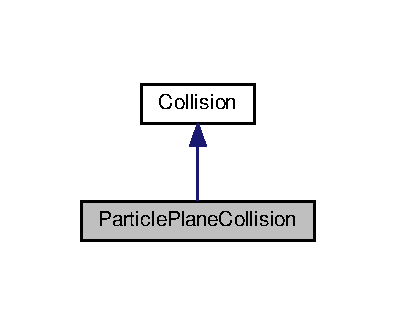
\includegraphics[width=190pt]{classParticlePlaneCollision__inherit__graph}
\end{center}
\end{figure}


Collaboration diagram for Particle\+Plane\+Collision\+:\nopagebreak
\begin{figure}[H]
\begin{center}
\leavevmode
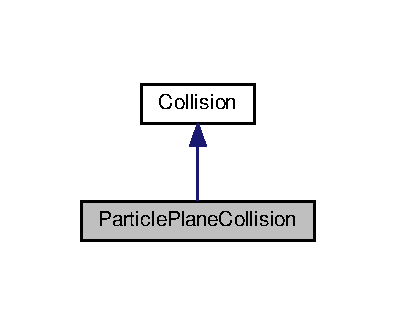
\includegraphics[width=190pt]{classParticlePlaneCollision__coll__graph}
\end{center}
\end{figure}
\subsection*{Public Member Functions}
\begin{DoxyCompactItemize}
\item 
\hyperlink{classParticlePlaneCollision_a155964653537ec6de0e91b25d3f7aa44}{$\sim$\+Particle\+Plane\+Collision} ()
\item 
\hyperlink{classParticlePlaneCollision_a5432307edb35e9762d9267c4146be9b3}{Particle\+Plane\+Collision} (\hyperlink{Particle_8hpp_a9a7abc8635002993537b61ef2c857fdd}{Particle\+Ptr} particle, \hyperlink{Plane_8hpp_a146e10989049e4a48eae6973c2f798f5}{Plane\+Ptr} plane, float restitution)
\begin{DoxyCompactList}\small\item\em Build a new collision event between a plane and a particle. \end{DoxyCompactList}\end{DoxyCompactItemize}
\subsection*{Private Member Functions}
\begin{DoxyCompactItemize}
\item 
void \hyperlink{classParticlePlaneCollision_a1516ee9898275c1ad9bfbc8bad675b1b}{do\+\_\+solve\+Collision} ()
\begin{DoxyCompactList}\small\item\em Solve the collision between the plane and the particle. \end{DoxyCompactList}\end{DoxyCompactItemize}
\subsection*{Private Attributes}
\begin{DoxyCompactItemize}
\item 
\hyperlink{Particle_8hpp_a9a7abc8635002993537b61ef2c857fdd}{Particle\+Ptr} \hyperlink{classParticlePlaneCollision_a26c423083839ce4155c62f422f03361b}{m\+\_\+particle}
\item 
\hyperlink{Plane_8hpp_a146e10989049e4a48eae6973c2f798f5}{Plane\+Ptr} \hyperlink{classParticlePlaneCollision_aad67527436168ca3413b7c7dba3f146c}{m\+\_\+plane}
\end{DoxyCompactItemize}
\subsection*{Additional Inherited Members}


\subsection{Detailed Description}
Implementation of the resolution of a collision event between a plane and a particle. 

\subsection{Constructor \& Destructor Documentation}
\hypertarget{classParticlePlaneCollision_a155964653537ec6de0e91b25d3f7aa44}{\index{Particle\+Plane\+Collision@{Particle\+Plane\+Collision}!````~Particle\+Plane\+Collision@{$\sim$\+Particle\+Plane\+Collision}}
\index{````~Particle\+Plane\+Collision@{$\sim$\+Particle\+Plane\+Collision}!Particle\+Plane\+Collision@{Particle\+Plane\+Collision}}
\subsubsection[{$\sim$\+Particle\+Plane\+Collision}]{\setlength{\rightskip}{0pt plus 5cm}Particle\+Plane\+Collision\+::$\sim$\+Particle\+Plane\+Collision (
\begin{DoxyParamCaption}
{}
\end{DoxyParamCaption}
)}}\label{classParticlePlaneCollision_a155964653537ec6de0e91b25d3f7aa44}
\hypertarget{classParticlePlaneCollision_a5432307edb35e9762d9267c4146be9b3}{\index{Particle\+Plane\+Collision@{Particle\+Plane\+Collision}!Particle\+Plane\+Collision@{Particle\+Plane\+Collision}}
\index{Particle\+Plane\+Collision@{Particle\+Plane\+Collision}!Particle\+Plane\+Collision@{Particle\+Plane\+Collision}}
\subsubsection[{Particle\+Plane\+Collision}]{\setlength{\rightskip}{0pt plus 5cm}Particle\+Plane\+Collision\+::\+Particle\+Plane\+Collision (
\begin{DoxyParamCaption}
\item[{{\bf Particle\+Ptr}}]{particle, }
\item[{{\bf Plane\+Ptr}}]{plane, }
\item[{float}]{restitution}
\end{DoxyParamCaption}
)}}\label{classParticlePlaneCollision_a5432307edb35e9762d9267c4146be9b3}
Build a collision event between a plane and a particle. This collision will be resolved assuming the plane is fixed. 
\begin{DoxyParams}{Parameters}
{\em particle} & The particle colliding a plane. \\
\hline
{\em plane} & The plane colliding a particle. \\
\hline
{\em restitution} & Restitution factor of this collision. \\
\hline
\end{DoxyParams}


\subsection{Member Function Documentation}
\hypertarget{classParticlePlaneCollision_a1516ee9898275c1ad9bfbc8bad675b1b}{\index{Particle\+Plane\+Collision@{Particle\+Plane\+Collision}!do\+\_\+solve\+Collision@{do\+\_\+solve\+Collision}}
\index{do\+\_\+solve\+Collision@{do\+\_\+solve\+Collision}!Particle\+Plane\+Collision@{Particle\+Plane\+Collision}}
\subsubsection[{do\+\_\+solve\+Collision}]{\setlength{\rightskip}{0pt plus 5cm}void Particle\+Plane\+Collision\+::do\+\_\+solve\+Collision (
\begin{DoxyParamCaption}
{}
\end{DoxyParamCaption}
)\hspace{0.3cm}{\ttfamily [private]}, {\ttfamily [virtual]}}}\label{classParticlePlaneCollision_a1516ee9898275c1ad9bfbc8bad675b1b}
Update the particle position and velocity after its collision with the fixed plane. 

Implements \hyperlink{classCollision_a5fa2b29df51abd8723660cd07050e616}{Collision}.



\subsection{Member Data Documentation}
\hypertarget{classParticlePlaneCollision_a26c423083839ce4155c62f422f03361b}{\index{Particle\+Plane\+Collision@{Particle\+Plane\+Collision}!m\+\_\+particle@{m\+\_\+particle}}
\index{m\+\_\+particle@{m\+\_\+particle}!Particle\+Plane\+Collision@{Particle\+Plane\+Collision}}
\subsubsection[{m\+\_\+particle}]{\setlength{\rightskip}{0pt plus 5cm}{\bf Particle\+Ptr} Particle\+Plane\+Collision\+::m\+\_\+particle\hspace{0.3cm}{\ttfamily [private]}}}\label{classParticlePlaneCollision_a26c423083839ce4155c62f422f03361b}
\hypertarget{classParticlePlaneCollision_aad67527436168ca3413b7c7dba3f146c}{\index{Particle\+Plane\+Collision@{Particle\+Plane\+Collision}!m\+\_\+plane@{m\+\_\+plane}}
\index{m\+\_\+plane@{m\+\_\+plane}!Particle\+Plane\+Collision@{Particle\+Plane\+Collision}}
\subsubsection[{m\+\_\+plane}]{\setlength{\rightskip}{0pt plus 5cm}{\bf Plane\+Ptr} Particle\+Plane\+Collision\+::m\+\_\+plane\hspace{0.3cm}{\ttfamily [private]}}}\label{classParticlePlaneCollision_aad67527436168ca3413b7c7dba3f146c}


The documentation for this class was generated from the following file\+:\begin{DoxyCompactItemize}
\item 
/home/chardon/\+Depot/ensimag/2\+A\+\_\+\+G3\+D/practicals/teacher\+Source/include/dynamics/\hyperlink{ParticlePlaneCollision_8hpp}{Particle\+Plane\+Collision.\+hpp}\end{DoxyCompactItemize}

\hypertarget{classParticleRenderable}{\section{Particle\+Renderable Class Reference}
\label{classParticleRenderable}\index{Particle\+Renderable@{Particle\+Renderable}}
}


Render a particle to the screen.  




{\ttfamily \#include $<$Particle\+Renderable.\+hpp$>$}



Inheritance diagram for Particle\+Renderable\+:\nopagebreak
\begin{figure}[H]
\begin{center}
\leavevmode
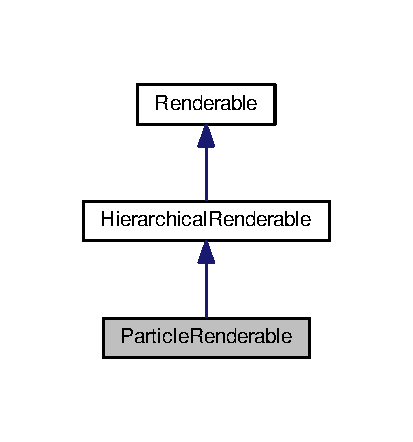
\includegraphics[width=198pt]{classParticleRenderable__inherit__graph}
\end{center}
\end{figure}


Collaboration diagram for Particle\+Renderable\+:\nopagebreak
\begin{figure}[H]
\begin{center}
\leavevmode
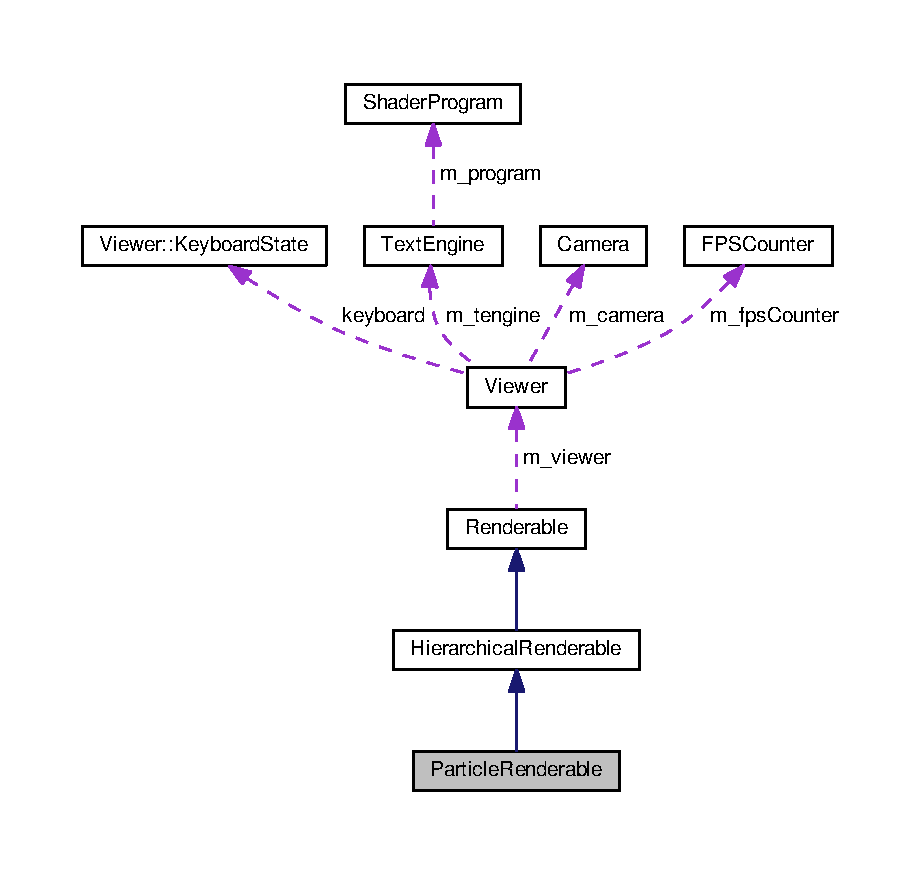
\includegraphics[width=350pt]{classParticleRenderable__coll__graph}
\end{center}
\end{figure}
\subsection*{Public Member Functions}
\begin{DoxyCompactItemize}
\item 
\hyperlink{classParticleRenderable_ab7f784b3520710e88d349a4c2f0f0ad1}{$\sim$\+Particle\+Renderable} ()
\item 
\hyperlink{classParticleRenderable_a3e5c194bb7e8f1470af0fc0e5d51e66e}{Particle\+Renderable} (\hyperlink{ShaderProgram_8hpp_af8e4af1ad4c53875ee5d32ab7e1f4966}{Shader\+Program\+Ptr} program, \hyperlink{Particle_8hpp_a9a7abc8635002993537b61ef2c857fdd}{Particle\+Ptr} particle)
\begin{DoxyCompactList}\small\item\em Build a particle renderable. \end{DoxyCompactList}\end{DoxyCompactItemize}
\subsection*{Private Member Functions}
\begin{DoxyCompactItemize}
\item 
void \hyperlink{classParticleRenderable_a1313290984b718988098504838fd4ee9}{do\+\_\+draw} ()
\begin{DoxyCompactList}\small\item\em Draw virtual function. \end{DoxyCompactList}\item 
void \hyperlink{classParticleRenderable_a8c4e33166ba0e4ee4cf1985eedea5aa3}{do\+\_\+animate} (float time)
\begin{DoxyCompactList}\small\item\em Animate virtual function. \end{DoxyCompactList}\end{DoxyCompactItemize}
\subsection*{Private Attributes}
\begin{DoxyCompactItemize}
\item 
\hyperlink{Particle_8hpp_a9a7abc8635002993537b61ef2c857fdd}{Particle\+Ptr} \hyperlink{classParticleRenderable_a40dd90b39f07278bfc9e5b9017c08592}{m\+\_\+particle}
\item 
std\+::vector$<$ glm\+::vec3 $>$ \hyperlink{classParticleRenderable_ae471301b0257ebc014ed7dabf16ebd16}{m\+\_\+positions}
\item 
std\+::vector$<$ glm\+::vec4 $>$ \hyperlink{classParticleRenderable_a8eb17ca66cfe99d7d23fe054d1ba14d5}{m\+\_\+colors}
\item 
std\+::vector$<$ glm\+::vec3 $>$ \hyperlink{classParticleRenderable_a816b9593b39a4f21d837bd0fbebd393e}{m\+\_\+normals}
\item 
unsigned int \hyperlink{classParticleRenderable_a42d3e2dc47524177be00fbc7ee1a244b}{m\+\_\+p\+Buffer}
\item 
unsigned int \hyperlink{classParticleRenderable_abe8e83a99746edd15b7611b8073c6ea9}{m\+\_\+c\+Buffer}
\item 
unsigned int \hyperlink{classParticleRenderable_adc8135a6d1f34037dcf942cf10cb296b}{m\+\_\+n\+Buffer}
\end{DoxyCompactItemize}
\subsection*{Additional Inherited Members}


\subsection{Detailed Description}
Render a particle to the screen. Since a particle is modeled by a ball, this renderable simply render the corresponding ball. If you have more than one renderable, have a look to \hyperlink{classParticleListRenderable}{Particle\+List\+Renderable}. 

\subsection{Constructor \& Destructor Documentation}
\hypertarget{classParticleRenderable_ab7f784b3520710e88d349a4c2f0f0ad1}{\index{Particle\+Renderable@{Particle\+Renderable}!````~Particle\+Renderable@{$\sim$\+Particle\+Renderable}}
\index{````~Particle\+Renderable@{$\sim$\+Particle\+Renderable}!Particle\+Renderable@{Particle\+Renderable}}
\subsubsection[{$\sim$\+Particle\+Renderable}]{\setlength{\rightskip}{0pt plus 5cm}Particle\+Renderable\+::$\sim$\+Particle\+Renderable (
\begin{DoxyParamCaption}
{}
\end{DoxyParamCaption}
)}}\label{classParticleRenderable_ab7f784b3520710e88d349a4c2f0f0ad1}
\hypertarget{classParticleRenderable_a3e5c194bb7e8f1470af0fc0e5d51e66e}{\index{Particle\+Renderable@{Particle\+Renderable}!Particle\+Renderable@{Particle\+Renderable}}
\index{Particle\+Renderable@{Particle\+Renderable}!Particle\+Renderable@{Particle\+Renderable}}
\subsubsection[{Particle\+Renderable}]{\setlength{\rightskip}{0pt plus 5cm}Particle\+Renderable\+::\+Particle\+Renderable (
\begin{DoxyParamCaption}
\item[{{\bf Shader\+Program\+Ptr}}]{program, }
\item[{{\bf Particle\+Ptr}}]{particle}
\end{DoxyParamCaption}
)}}\label{classParticleRenderable_a3e5c194bb7e8f1470af0fc0e5d51e66e}
Build a renderable to render a particle. 
\begin{DoxyParams}{Parameters}
{\em program} & The shader program used to render the particle. \\
\hline
{\em particle} & The particle to render. \\
\hline
\end{DoxyParams}


\subsection{Member Function Documentation}
\hypertarget{classParticleRenderable_a8c4e33166ba0e4ee4cf1985eedea5aa3}{\index{Particle\+Renderable@{Particle\+Renderable}!do\+\_\+animate@{do\+\_\+animate}}
\index{do\+\_\+animate@{do\+\_\+animate}!Particle\+Renderable@{Particle\+Renderable}}
\subsubsection[{do\+\_\+animate}]{\setlength{\rightskip}{0pt plus 5cm}void Particle\+Renderable\+::do\+\_\+animate (
\begin{DoxyParamCaption}
\item[{float}]{time}
\end{DoxyParamCaption}
)\hspace{0.3cm}{\ttfamily [private]}, {\ttfamily [virtual]}}}\label{classParticleRenderable_a8c4e33166ba0e4ee4cf1985eedea5aa3}
Implementation to animate this renderable. 
\begin{DoxyParams}{Parameters}
{\em time} & The current simulation time. \\
\hline
\end{DoxyParams}


Implements \hyperlink{classRenderable_aa5206322555c9dece40b21e797629b34}{Renderable}.

\hypertarget{classParticleRenderable_a1313290984b718988098504838fd4ee9}{\index{Particle\+Renderable@{Particle\+Renderable}!do\+\_\+draw@{do\+\_\+draw}}
\index{do\+\_\+draw@{do\+\_\+draw}!Particle\+Renderable@{Particle\+Renderable}}
\subsubsection[{do\+\_\+draw}]{\setlength{\rightskip}{0pt plus 5cm}void Particle\+Renderable\+::do\+\_\+draw (
\begin{DoxyParamCaption}
{}
\end{DoxyParamCaption}
)\hspace{0.3cm}{\ttfamily [private]}, {\ttfamily [virtual]}}}\label{classParticleRenderable_a1313290984b718988098504838fd4ee9}
Implementation to draw this renderable. 

Implements \hyperlink{classRenderable_a98ab6308c1d2b56dacda7c435fb38d5b}{Renderable}.



\subsection{Member Data Documentation}
\hypertarget{classParticleRenderable_abe8e83a99746edd15b7611b8073c6ea9}{\index{Particle\+Renderable@{Particle\+Renderable}!m\+\_\+c\+Buffer@{m\+\_\+c\+Buffer}}
\index{m\+\_\+c\+Buffer@{m\+\_\+c\+Buffer}!Particle\+Renderable@{Particle\+Renderable}}
\subsubsection[{m\+\_\+c\+Buffer}]{\setlength{\rightskip}{0pt plus 5cm}unsigned int Particle\+Renderable\+::m\+\_\+c\+Buffer\hspace{0.3cm}{\ttfamily [private]}}}\label{classParticleRenderable_abe8e83a99746edd15b7611b8073c6ea9}
\hypertarget{classParticleRenderable_a8eb17ca66cfe99d7d23fe054d1ba14d5}{\index{Particle\+Renderable@{Particle\+Renderable}!m\+\_\+colors@{m\+\_\+colors}}
\index{m\+\_\+colors@{m\+\_\+colors}!Particle\+Renderable@{Particle\+Renderable}}
\subsubsection[{m\+\_\+colors}]{\setlength{\rightskip}{0pt plus 5cm}std\+::vector$<$ glm\+::vec4 $>$ Particle\+Renderable\+::m\+\_\+colors\hspace{0.3cm}{\ttfamily [private]}}}\label{classParticleRenderable_a8eb17ca66cfe99d7d23fe054d1ba14d5}
\hypertarget{classParticleRenderable_adc8135a6d1f34037dcf942cf10cb296b}{\index{Particle\+Renderable@{Particle\+Renderable}!m\+\_\+n\+Buffer@{m\+\_\+n\+Buffer}}
\index{m\+\_\+n\+Buffer@{m\+\_\+n\+Buffer}!Particle\+Renderable@{Particle\+Renderable}}
\subsubsection[{m\+\_\+n\+Buffer}]{\setlength{\rightskip}{0pt plus 5cm}unsigned int Particle\+Renderable\+::m\+\_\+n\+Buffer\hspace{0.3cm}{\ttfamily [private]}}}\label{classParticleRenderable_adc8135a6d1f34037dcf942cf10cb296b}
\hypertarget{classParticleRenderable_a816b9593b39a4f21d837bd0fbebd393e}{\index{Particle\+Renderable@{Particle\+Renderable}!m\+\_\+normals@{m\+\_\+normals}}
\index{m\+\_\+normals@{m\+\_\+normals}!Particle\+Renderable@{Particle\+Renderable}}
\subsubsection[{m\+\_\+normals}]{\setlength{\rightskip}{0pt plus 5cm}std\+::vector$<$ glm\+::vec3 $>$ Particle\+Renderable\+::m\+\_\+normals\hspace{0.3cm}{\ttfamily [private]}}}\label{classParticleRenderable_a816b9593b39a4f21d837bd0fbebd393e}
\hypertarget{classParticleRenderable_a40dd90b39f07278bfc9e5b9017c08592}{\index{Particle\+Renderable@{Particle\+Renderable}!m\+\_\+particle@{m\+\_\+particle}}
\index{m\+\_\+particle@{m\+\_\+particle}!Particle\+Renderable@{Particle\+Renderable}}
\subsubsection[{m\+\_\+particle}]{\setlength{\rightskip}{0pt plus 5cm}{\bf Particle\+Ptr} Particle\+Renderable\+::m\+\_\+particle\hspace{0.3cm}{\ttfamily [private]}}}\label{classParticleRenderable_a40dd90b39f07278bfc9e5b9017c08592}
\hypertarget{classParticleRenderable_a42d3e2dc47524177be00fbc7ee1a244b}{\index{Particle\+Renderable@{Particle\+Renderable}!m\+\_\+p\+Buffer@{m\+\_\+p\+Buffer}}
\index{m\+\_\+p\+Buffer@{m\+\_\+p\+Buffer}!Particle\+Renderable@{Particle\+Renderable}}
\subsubsection[{m\+\_\+p\+Buffer}]{\setlength{\rightskip}{0pt plus 5cm}unsigned int Particle\+Renderable\+::m\+\_\+p\+Buffer\hspace{0.3cm}{\ttfamily [private]}}}\label{classParticleRenderable_a42d3e2dc47524177be00fbc7ee1a244b}
\hypertarget{classParticleRenderable_ae471301b0257ebc014ed7dabf16ebd16}{\index{Particle\+Renderable@{Particle\+Renderable}!m\+\_\+positions@{m\+\_\+positions}}
\index{m\+\_\+positions@{m\+\_\+positions}!Particle\+Renderable@{Particle\+Renderable}}
\subsubsection[{m\+\_\+positions}]{\setlength{\rightskip}{0pt plus 5cm}std\+::vector$<$ glm\+::vec3 $>$ Particle\+Renderable\+::m\+\_\+positions\hspace{0.3cm}{\ttfamily [private]}}}\label{classParticleRenderable_ae471301b0257ebc014ed7dabf16ebd16}


The documentation for this class was generated from the following file\+:\begin{DoxyCompactItemize}
\item 
/home/chardon/\+Depot/ensimag/2\+A\+\_\+\+G3\+D/practicals/teacher\+Source/include/dynamics/\hyperlink{ParticleRenderable_8hpp}{Particle\+Renderable.\+hpp}\end{DoxyCompactItemize}

\hypertarget{classPlane}{\section{Plane Class Reference}
\label{classPlane}\index{Plane@{Plane}}
}


Geometry representation of an infinite plane.  




{\ttfamily \#include $<$Plane.\+hpp$>$}

\subsection*{Public Member Functions}
\begin{DoxyCompactItemize}
\item 
\hyperlink{classPlane_ab0a2674b0b2a14afaf71c34392e5d374}{Plane} (const glm\+::vec3 \&\hyperlink{classPlane_afea6480f0bbab2a9ef0c74bd7af5d595}{normal}, const glm\+::vec3 \&point)
\begin{DoxyCompactList}\small\item\em Build a plane with a normal and a point. \end{DoxyCompactList}\item 
\hyperlink{classPlane_adccfb4ea49813a45fd883438af858495}{Plane} (const glm\+::vec3 \&a, const glm\+::vec3 \&b, const glm\+::vec3 \&c)
\begin{DoxyCompactList}\small\item\em Build the plane passing through three points. \end{DoxyCompactList}\item 
void \hyperlink{classPlane_aa299ec4054d6735e8f2fffde2a38b434}{set\+Distance\+To\+Origin} (const float \&d)
\begin{DoxyCompactList}\small\item\em Manually set the distance from this plane to the origin. \end{DoxyCompactList}\item 
const float \& \hyperlink{classPlane_aeec90982ee9dd4a1d47d3570374ffbc0}{distance\+To\+Origin} () const 
\begin{DoxyCompactList}\small\item\em Access to the distance to the origin. \end{DoxyCompactList}\item 
void \hyperlink{classPlane_a1cddc7028e96d68a176fb742ab1e349d}{set\+Normal} (const glm\+::vec3 \&n)
\begin{DoxyCompactList}\small\item\em Set the plane's normal. \end{DoxyCompactList}\item 
const glm\+::vec3 \& \hyperlink{classPlane_afea6480f0bbab2a9ef0c74bd7af5d595}{normal} () const 
\begin{DoxyCompactList}\small\item\em Access the plane's normal. \end{DoxyCompactList}\item 
glm\+::vec3 \hyperlink{classPlane_ac8f889e4cfc5c30a379c516b22cda15b}{project\+On\+Plane} (const glm\+::vec3 \&p)
\begin{DoxyCompactList}\small\item\em Get the projection of a point on this plane. \end{DoxyCompactList}\end{DoxyCompactItemize}
\subsection*{Private Attributes}
\begin{DoxyCompactItemize}
\item 
glm\+::vec3 \hyperlink{classPlane_a47fca7e21a0e825f754182692fad45b0}{m\+\_\+n}
\item 
float \hyperlink{classPlane_a5864bedfa1eb0ff017b89631fc7aff01}{m\+\_\+d}
\end{DoxyCompactItemize}


\subsection{Detailed Description}
Represent an infinite plane. 

\subsection{Constructor \& Destructor Documentation}
\hypertarget{classPlane_ab0a2674b0b2a14afaf71c34392e5d374}{\index{Plane@{Plane}!Plane@{Plane}}
\index{Plane@{Plane}!Plane@{Plane}}
\subsubsection[{Plane}]{\setlength{\rightskip}{0pt plus 5cm}Plane\+::\+Plane (
\begin{DoxyParamCaption}
\item[{const glm\+::vec3 \&}]{normal, }
\item[{const glm\+::vec3 \&}]{point}
\end{DoxyParamCaption}
)}}\label{classPlane_ab0a2674b0b2a14afaf71c34392e5d374}
Build a plane normal to the specified normal, passing by a particular point. 
\begin{DoxyParams}{Parameters}
{\em normal} & The normal of the plane \\
\hline
{\em point} & A point belonging to the plane. \\
\hline
\end{DoxyParams}
\hypertarget{classPlane_adccfb4ea49813a45fd883438af858495}{\index{Plane@{Plane}!Plane@{Plane}}
\index{Plane@{Plane}!Plane@{Plane}}
\subsubsection[{Plane}]{\setlength{\rightskip}{0pt plus 5cm}Plane\+::\+Plane (
\begin{DoxyParamCaption}
\item[{const glm\+::vec3 \&}]{a, }
\item[{const glm\+::vec3 \&}]{b, }
\item[{const glm\+::vec3 \&}]{c}
\end{DoxyParamCaption}
)}}\label{classPlane_adccfb4ea49813a45fd883438af858495}
Build a plane containing three points. 
\begin{DoxyParams}{Parameters}
{\em a} & The first point belonging to the plane. \\
\hline
{\em b} & The second point belonging to the plane. \\
\hline
{\em c} & The third point belonging to the plane. \\
\hline
\end{DoxyParams}


\subsection{Member Function Documentation}
\hypertarget{classPlane_aeec90982ee9dd4a1d47d3570374ffbc0}{\index{Plane@{Plane}!distance\+To\+Origin@{distance\+To\+Origin}}
\index{distance\+To\+Origin@{distance\+To\+Origin}!Plane@{Plane}}
\subsubsection[{distance\+To\+Origin}]{\setlength{\rightskip}{0pt plus 5cm}const float\& Plane\+::distance\+To\+Origin (
\begin{DoxyParamCaption}
{}
\end{DoxyParamCaption}
) const}}\label{classPlane_aeec90982ee9dd4a1d47d3570374ffbc0}
Get the distance between this plane and the origin. \begin{DoxyReturn}{Returns}
The distance to the origin. 
\end{DoxyReturn}
\hypertarget{classPlane_afea6480f0bbab2a9ef0c74bd7af5d595}{\index{Plane@{Plane}!normal@{normal}}
\index{normal@{normal}!Plane@{Plane}}
\subsubsection[{normal}]{\setlength{\rightskip}{0pt plus 5cm}const glm\+::vec3\& Plane\+::normal (
\begin{DoxyParamCaption}
{}
\end{DoxyParamCaption}
) const}}\label{classPlane_afea6480f0bbab2a9ef0c74bd7af5d595}
Get the plane's normal. \begin{DoxyReturn}{Returns}
The plane's normal. 
\end{DoxyReturn}
\hypertarget{classPlane_ac8f889e4cfc5c30a379c516b22cda15b}{\index{Plane@{Plane}!project\+On\+Plane@{project\+On\+Plane}}
\index{project\+On\+Plane@{project\+On\+Plane}!Plane@{Plane}}
\subsubsection[{project\+On\+Plane}]{\setlength{\rightskip}{0pt plus 5cm}glm\+::vec3 Plane\+::project\+On\+Plane (
\begin{DoxyParamCaption}
\item[{const glm\+::vec3 \&}]{p}
\end{DoxyParamCaption}
)}}\label{classPlane_ac8f889e4cfc5c30a379c516b22cda15b}
Get the orthogonal projection of a point on this plane. 
\begin{DoxyParams}{Parameters}
{\em p} & The point to project. \\
\hline
\end{DoxyParams}
\begin{DoxyReturn}{Returns}
The orthogonal projection of p. 
\end{DoxyReturn}
\hypertarget{classPlane_aa299ec4054d6735e8f2fffde2a38b434}{\index{Plane@{Plane}!set\+Distance\+To\+Origin@{set\+Distance\+To\+Origin}}
\index{set\+Distance\+To\+Origin@{set\+Distance\+To\+Origin}!Plane@{Plane}}
\subsubsection[{set\+Distance\+To\+Origin}]{\setlength{\rightskip}{0pt plus 5cm}void Plane\+::set\+Distance\+To\+Origin (
\begin{DoxyParamCaption}
\item[{const float \&}]{d}
\end{DoxyParamCaption}
)}}\label{classPlane_aa299ec4054d6735e8f2fffde2a38b434}
Set the distance min\+\_\+(p in this) $\vert$$\vert$ p -\/ vec3(0,0,0) $\vert$$\vert$. 
\begin{DoxyParams}{Parameters}
{\em d} & New distance to the origin. \\
\hline
\end{DoxyParams}
\hypertarget{classPlane_a1cddc7028e96d68a176fb742ab1e349d}{\index{Plane@{Plane}!set\+Normal@{set\+Normal}}
\index{set\+Normal@{set\+Normal}!Plane@{Plane}}
\subsubsection[{set\+Normal}]{\setlength{\rightskip}{0pt plus 5cm}void Plane\+::set\+Normal (
\begin{DoxyParamCaption}
\item[{const glm\+::vec3 \&}]{n}
\end{DoxyParamCaption}
)}}\label{classPlane_a1cddc7028e96d68a176fb742ab1e349d}
Set the plane's normal. 
\begin{DoxyParams}{Parameters}
{\em n} & The new plane's normal. \\
\hline
\end{DoxyParams}


\subsection{Member Data Documentation}
\hypertarget{classPlane_a5864bedfa1eb0ff017b89631fc7aff01}{\index{Plane@{Plane}!m\+\_\+d@{m\+\_\+d}}
\index{m\+\_\+d@{m\+\_\+d}!Plane@{Plane}}
\subsubsection[{m\+\_\+d}]{\setlength{\rightskip}{0pt plus 5cm}float Plane\+::m\+\_\+d\hspace{0.3cm}{\ttfamily [private]}}}\label{classPlane_a5864bedfa1eb0ff017b89631fc7aff01}
m\+\_\+d = dot(m\+\_\+n,p) for a given point p on the plane \hypertarget{classPlane_a47fca7e21a0e825f754182692fad45b0}{\index{Plane@{Plane}!m\+\_\+n@{m\+\_\+n}}
\index{m\+\_\+n@{m\+\_\+n}!Plane@{Plane}}
\subsubsection[{m\+\_\+n}]{\setlength{\rightskip}{0pt plus 5cm}glm\+::vec3 Plane\+::m\+\_\+n\hspace{0.3cm}{\ttfamily [private]}}}\label{classPlane_a47fca7e21a0e825f754182692fad45b0}
\hyperlink{classPlane}{Plane} normal. Points x on the plane satisfy dot(m\+\_\+n,x)=m\+\_\+d 

The documentation for this class was generated from the following file\+:\begin{DoxyCompactItemize}
\item 
/home/chardon/\+Depot/ensimag/2\+A\+\_\+\+G3\+D/practicals/teacher\+Source/include/\hyperlink{Plane_8hpp}{Plane.\+hpp}\end{DoxyCompactItemize}

\hypertarget{classPointLight}{\section{Point\+Light Class Reference}
\label{classPointLight}\index{Point\+Light@{Point\+Light}}
}


A point light.  




{\ttfamily \#include $<$Light.\+hpp$>$}

\subsection*{Public Types}
\begin{DoxyCompactItemize}
\item 
typedef std\+::shared\+\_\+ptr\\*
$<$ \hyperlink{classPointLight}{Point\+Light} $>$ \hyperlink{classPointLight_a48c8893ebd8015da2cb3d552f800e4e7}{Point\+Light\+Ptr}
\end{DoxyCompactItemize}
\subsection*{Public Member Functions}
\begin{DoxyCompactItemize}
\item 
\hyperlink{classPointLight_aa12d9005d5372dbbe655a82231634341}{$\sim$\+Point\+Light} ()
\begin{DoxyCompactList}\small\item\em Destructor. \end{DoxyCompactList}\item 
\hyperlink{classPointLight_abbfdf5f05b559c49016f8bb97b0ca414}{Point\+Light} ()
\begin{DoxyCompactList}\small\item\em Default constructor. \end{DoxyCompactList}\item 
\hyperlink{classPointLight_a85e984228a1967b53114378b46a8f80a}{Point\+Light} (const \hyperlink{classPointLight}{Point\+Light} \&point\+Light)
\begin{DoxyCompactList}\small\item\em Default constructor. \end{DoxyCompactList}\item 
\hyperlink{classPointLight_a813f361fa033b13412a4c2268263b4de}{Point\+Light} (const glm\+::vec3 \&\hyperlink{classPointLight_a46ba05eb1117e13cf078fa0fe4d1579f}{position}, const glm\+::vec3 \&\hyperlink{classPointLight_a80a915d16e9b7576107ce23318c0d547}{ambient}, const glm\+::vec3 \&\hyperlink{classPointLight_a35474dabe9643e96eff5447f14b41a7b}{diffuse}, const glm\+::vec3 \&\hyperlink{classPointLight_aedd6ede28b41d05e277c26fcbfa1657d}{specular}, const float \&\hyperlink{classPointLight_afa1541cdc95ff0e7283c545e4aec2737}{constant}, const float \&\hyperlink{classPointLight_ad79e03bc6d87477bf0d2f00866531f6c}{linear}, const float \&\hyperlink{classPointLight_ac531ddcb6a17371501f30af9474c7d8c}{quadratic})
\begin{DoxyCompactList}\small\item\em Specific constructor. \end{DoxyCompactList}\item 
const glm\+::vec3 \& \hyperlink{classPointLight_a46ba05eb1117e13cf078fa0fe4d1579f}{position} () const 
\begin{DoxyCompactList}\small\item\em Access to the position of the light. \end{DoxyCompactList}\item 
void \hyperlink{classPointLight_a17a969466c4c0fafca34f45b8984c11b}{set\+Position} (const glm\+::vec3 \&\hyperlink{classPointLight_a46ba05eb1117e13cf078fa0fe4d1579f}{position})
\begin{DoxyCompactList}\small\item\em Set the position of the light. \end{DoxyCompactList}\item 
const glm\+::vec3 \& \hyperlink{classPointLight_a80a915d16e9b7576107ce23318c0d547}{ambient} () const 
\begin{DoxyCompactList}\small\item\em Access to the ambient intensity of the light. \end{DoxyCompactList}\item 
void \hyperlink{classPointLight_adfb7c1860bdf0c2311a148fd0045cea7}{set\+Ambient} (const glm\+::vec3 \&\hyperlink{classPointLight_a80a915d16e9b7576107ce23318c0d547}{ambient})
\begin{DoxyCompactList}\small\item\em Set the ambient intensity of the light. \end{DoxyCompactList}\item 
const glm\+::vec3 \& \hyperlink{classPointLight_a35474dabe9643e96eff5447f14b41a7b}{diffuse} () const 
\begin{DoxyCompactList}\small\item\em Access to the diffuse intensity of the light. \end{DoxyCompactList}\item 
void \hyperlink{classPointLight_a85de8464abaf20336e9f98f7ad48a638}{set\+Diffuse} (const glm\+::vec3 \&\hyperlink{classPointLight_a35474dabe9643e96eff5447f14b41a7b}{diffuse})
\begin{DoxyCompactList}\small\item\em Set the diffuse intensity of the light. \end{DoxyCompactList}\item 
const glm\+::vec3 \& \hyperlink{classPointLight_aedd6ede28b41d05e277c26fcbfa1657d}{specular} () const 
\begin{DoxyCompactList}\small\item\em Access to the specular intensity of the light. \end{DoxyCompactList}\item 
void \hyperlink{classPointLight_a7265b55493251009964a44debc40d85d}{set\+Specular} (const glm\+::vec3 \&\hyperlink{classPointLight_aedd6ede28b41d05e277c26fcbfa1657d}{specular})
\begin{DoxyCompactList}\small\item\em Set the specular intensity of the light. \end{DoxyCompactList}\item 
const float \& \hyperlink{classPointLight_afa1541cdc95ff0e7283c545e4aec2737}{constant} () const 
\begin{DoxyCompactList}\small\item\em Access to the coefficient of constant attenuation of the light. \end{DoxyCompactList}\item 
void \hyperlink{classPointLight_aa72656b486eab2403eb113a4c6a8161e}{set\+Constant} (float \hyperlink{classPointLight_afa1541cdc95ff0e7283c545e4aec2737}{constant})
\begin{DoxyCompactList}\small\item\em Set the coefficient of constant attenuation of the light. \end{DoxyCompactList}\item 
const float \& \hyperlink{classPointLight_ad79e03bc6d87477bf0d2f00866531f6c}{linear} () const 
\begin{DoxyCompactList}\small\item\em Access to the coefficient of linear attenuation of the light. \end{DoxyCompactList}\item 
void \hyperlink{classPointLight_a91369fd3b2e7717f529faf8b2ac94e57}{set\+Linear} (float \hyperlink{classPointLight_ad79e03bc6d87477bf0d2f00866531f6c}{linear})
\begin{DoxyCompactList}\small\item\em Set the coefficient of linear attenuation of the light. \end{DoxyCompactList}\item 
const float \& \hyperlink{classPointLight_ac531ddcb6a17371501f30af9474c7d8c}{quadratic} () const 
\begin{DoxyCompactList}\small\item\em Access to the coefficient of quadratic attenuation of the light. \end{DoxyCompactList}\item 
void \hyperlink{classPointLight_a0807e355fe3e00173010539f501e75b1}{set\+Quadratic} (float \hyperlink{classPointLight_ac531ddcb6a17371501f30af9474c7d8c}{quadratic})
\begin{DoxyCompactList}\small\item\em Set the coefficient of quadratic attenuation of the light. \end{DoxyCompactList}\end{DoxyCompactItemize}
\subsection*{Static Public Member Functions}
\begin{DoxyCompactItemize}
\item 
static bool \hyperlink{classPointLight_a09784e83b307a49218362dedd46b3f45}{send\+To\+G\+P\+U} (const \hyperlink{ShaderProgram_8hpp_af8e4af1ad4c53875ee5d32ab7e1f4966}{Shader\+Program\+Ptr} \&program, const \hyperlink{classPointLight_a48c8893ebd8015da2cb3d552f800e4e7}{Point\+Light\+Ptr} \&light)
\begin{DoxyCompactList}\small\item\em Get location for the attributes of the light and send the data to the G\+P\+U as uniforms. \end{DoxyCompactList}\item 
static bool \hyperlink{classPointLight_a01a877269592617f8280ed9be418b612}{send\+To\+G\+P\+U} (const \hyperlink{ShaderProgram_8hpp_af8e4af1ad4c53875ee5d32ab7e1f4966}{Shader\+Program\+Ptr} \&program, const std\+::vector$<$ \hyperlink{classPointLight_a48c8893ebd8015da2cb3d552f800e4e7}{Point\+Light\+Ptr} $>$ \&lights)
\begin{DoxyCompactList}\small\item\em Get location for the attributes of the lights and send the data to the G\+P\+U as uniforms. \end{DoxyCompactList}\end{DoxyCompactItemize}
\subsection*{Private Member Functions}
\begin{DoxyCompactItemize}
\item 
std\+::string \hyperlink{classPointLight_a52eca397963df514af41178aec06dacf}{number\+Of\+Lights\+Name} ()
\begin{DoxyCompactList}\small\item\em Get the uniform name of the number of lights. \end{DoxyCompactList}\item 
std\+::string \hyperlink{classPointLight_a7c797f6ef8ae47d4ba86747731ed1e91}{light\+Name} ()
\begin{DoxyCompactList}\small\item\em Get the uniform name of the light. \end{DoxyCompactList}\item 
std\+::string \hyperlink{classPointLight_a270bf32badcf99da825c752ade0fca03}{position\+Name} ()
\begin{DoxyCompactList}\small\item\em Get the uniform name of the position of the light. \end{DoxyCompactList}\item 
std\+::string \hyperlink{classPointLight_a7a164908b6773d1607d303d7a05e9370}{ambient\+Name} ()
\begin{DoxyCompactList}\small\item\em Get the uniform name of the ambient intensity of the light. \end{DoxyCompactList}\item 
std\+::string \hyperlink{classPointLight_a8aa0ba053b1c4b5a4a6525dc94f1298b}{diffuse\+Name} ()
\begin{DoxyCompactList}\small\item\em Get the uniform name of the diffuse intensity of the light. \end{DoxyCompactList}\item 
std\+::string \hyperlink{classPointLight_a7f02ce1e373b96b445916db3c7397921}{specular\+Name} ()
\begin{DoxyCompactList}\small\item\em Get the uniform name of the specular intensity of the light. \end{DoxyCompactList}\item 
std\+::string \hyperlink{classPointLight_a4b08c94d77d9b1d8b858ecf834bb4aa6}{constant\+Name} ()
\begin{DoxyCompactList}\small\item\em Get the uniform name of the constant attenuation coefficient of the light. \end{DoxyCompactList}\item 
std\+::string \hyperlink{classPointLight_a505d362ac12ed47b169aced70f646bd4}{linear\+Name} ()
\begin{DoxyCompactList}\small\item\em Get the uniform name of the linear attenuation coefficient of the light. \end{DoxyCompactList}\item 
std\+::string \hyperlink{classPointLight_a86032735679d386e6c3d94540767adab}{quadratic\+Name} ()
\begin{DoxyCompactList}\small\item\em Get the uniform name of the quadratic attenuation coefficient of the light. \end{DoxyCompactList}\end{DoxyCompactItemize}
\subsection*{Private Attributes}
\begin{DoxyCompactItemize}
\item 
glm\+::vec3 \hyperlink{classPointLight_a58baecb4dd64a4dc3ea59628f55cbac4}{m\+\_\+position}
\item 
glm\+::vec3 \hyperlink{classPointLight_a24fea5d1cc566b9a5266e3fc2df56f22}{m\+\_\+ambient}
\item 
glm\+::vec3 \hyperlink{classPointLight_a3e055011470b6dc9000f57fde449b8e2}{m\+\_\+diffuse}
\item 
glm\+::vec3 \hyperlink{classPointLight_a07a85987190c6c415b93437554f1f0f1}{m\+\_\+specular}
\item 
float \hyperlink{classPointLight_a404f6e39448eaa92dbdbec6183062147}{m\+\_\+constant}
\item 
float \hyperlink{classPointLight_aaaf19c31763c3614e3edcd1eef322e96}{m\+\_\+linear}
\item 
float \hyperlink{classPointLight_a4cc1b2791d8e3ca503060f6f1f38f774}{m\+\_\+quadratic}
\end{DoxyCompactItemize}


\subsection{Detailed Description}
This class represents a point light which means a light with a given position somewhere in a world that illuminates in all directions. Good examples of point light are torches. 

\subsection{Member Typedef Documentation}
\hypertarget{classPointLight_a48c8893ebd8015da2cb3d552f800e4e7}{\index{Point\+Light@{Point\+Light}!Point\+Light\+Ptr@{Point\+Light\+Ptr}}
\index{Point\+Light\+Ptr@{Point\+Light\+Ptr}!Point\+Light@{Point\+Light}}
\subsubsection[{Point\+Light\+Ptr}]{\setlength{\rightskip}{0pt plus 5cm}typedef std\+::shared\+\_\+ptr$<${\bf Point\+Light}$>$ {\bf Point\+Light\+::\+Point\+Light\+Ptr}}}\label{classPointLight_a48c8893ebd8015da2cb3d552f800e4e7}
Smart pointer to a point light 

\subsection{Constructor \& Destructor Documentation}
\hypertarget{classPointLight_aa12d9005d5372dbbe655a82231634341}{\index{Point\+Light@{Point\+Light}!````~Point\+Light@{$\sim$\+Point\+Light}}
\index{````~Point\+Light@{$\sim$\+Point\+Light}!Point\+Light@{Point\+Light}}
\subsubsection[{$\sim$\+Point\+Light}]{\setlength{\rightskip}{0pt plus 5cm}Point\+Light\+::$\sim$\+Point\+Light (
\begin{DoxyParamCaption}
{}
\end{DoxyParamCaption}
)}}\label{classPointLight_aa12d9005d5372dbbe655a82231634341}
\hypertarget{classPointLight_abbfdf5f05b559c49016f8bb97b0ca414}{\index{Point\+Light@{Point\+Light}!Point\+Light@{Point\+Light}}
\index{Point\+Light@{Point\+Light}!Point\+Light@{Point\+Light}}
\subsubsection[{Point\+Light}]{\setlength{\rightskip}{0pt plus 5cm}Point\+Light\+::\+Point\+Light (
\begin{DoxyParamCaption}
{}
\end{DoxyParamCaption}
)}}\label{classPointLight_abbfdf5f05b559c49016f8bb97b0ca414}
\hypertarget{classPointLight_a85e984228a1967b53114378b46a8f80a}{\index{Point\+Light@{Point\+Light}!Point\+Light@{Point\+Light}}
\index{Point\+Light@{Point\+Light}!Point\+Light@{Point\+Light}}
\subsubsection[{Point\+Light}]{\setlength{\rightskip}{0pt plus 5cm}Point\+Light\+::\+Point\+Light (
\begin{DoxyParamCaption}
\item[{const {\bf Point\+Light} \&}]{point\+Light}
\end{DoxyParamCaption}
)}}\label{classPointLight_a85e984228a1967b53114378b46a8f80a}
\hypertarget{classPointLight_a813f361fa033b13412a4c2268263b4de}{\index{Point\+Light@{Point\+Light}!Point\+Light@{Point\+Light}}
\index{Point\+Light@{Point\+Light}!Point\+Light@{Point\+Light}}
\subsubsection[{Point\+Light}]{\setlength{\rightskip}{0pt plus 5cm}Point\+Light\+::\+Point\+Light (
\begin{DoxyParamCaption}
\item[{const glm\+::vec3 \&}]{position, }
\item[{const glm\+::vec3 \&}]{ambient, }
\item[{const glm\+::vec3 \&}]{diffuse, }
\item[{const glm\+::vec3 \&}]{specular, }
\item[{const float \&}]{constant, }
\item[{const float \&}]{linear, }
\item[{const float \&}]{quadratic}
\end{DoxyParamCaption}
)}}\label{classPointLight_a813f361fa033b13412a4c2268263b4de}
Construct a point light.


\begin{DoxyParams}{Parameters}
{\em position} & The position of the light. \\
\hline
{\em ambient} & The ambient intensity of the light. \\
\hline
{\em diffuse} & The diffuse intensity of the light. \\
\hline
{\em specular} & The specular intensity of the light. \\
\hline
{\em constant} & The coefficient of constant attenuation of the light. \\
\hline
{\em linear} & The coefficient of linear attenuation of the light with respect to the distance to the light. \\
\hline
{\em quadratic} & The coefficient of quadratic attenuation of the light with respect to the distance to the light. \\
\hline
\end{DoxyParams}


\subsection{Member Function Documentation}
\hypertarget{classPointLight_a80a915d16e9b7576107ce23318c0d547}{\index{Point\+Light@{Point\+Light}!ambient@{ambient}}
\index{ambient@{ambient}!Point\+Light@{Point\+Light}}
\subsubsection[{ambient}]{\setlength{\rightskip}{0pt plus 5cm}const glm\+::vec3\& Point\+Light\+::ambient (
\begin{DoxyParamCaption}
{}
\end{DoxyParamCaption}
) const}}\label{classPointLight_a80a915d16e9b7576107ce23318c0d547}
\begin{DoxyReturn}{Returns}
A const reference to m\+\_\+ambient. 
\end{DoxyReturn}
\hypertarget{classPointLight_a7a164908b6773d1607d303d7a05e9370}{\index{Point\+Light@{Point\+Light}!ambient\+Name@{ambient\+Name}}
\index{ambient\+Name@{ambient\+Name}!Point\+Light@{Point\+Light}}
\subsubsection[{ambient\+Name}]{\setlength{\rightskip}{0pt plus 5cm}std\+::string Point\+Light\+::ambient\+Name (
\begin{DoxyParamCaption}
{}
\end{DoxyParamCaption}
)\hspace{0.3cm}{\ttfamily [inline]}, {\ttfamily [private]}}}\label{classPointLight_a7a164908b6773d1607d303d7a05e9370}
\begin{DoxyReturn}{Returns}
The name of the ambient intensity of the light in the shader. 
\end{DoxyReturn}
\hypertarget{classPointLight_afa1541cdc95ff0e7283c545e4aec2737}{\index{Point\+Light@{Point\+Light}!constant@{constant}}
\index{constant@{constant}!Point\+Light@{Point\+Light}}
\subsubsection[{constant}]{\setlength{\rightskip}{0pt plus 5cm}const float\& Point\+Light\+::constant (
\begin{DoxyParamCaption}
{}
\end{DoxyParamCaption}
) const}}\label{classPointLight_afa1541cdc95ff0e7283c545e4aec2737}
\begin{DoxyReturn}{Returns}
A const reference to m\+\_\+constant. 
\end{DoxyReturn}
\hypertarget{classPointLight_a4b08c94d77d9b1d8b858ecf834bb4aa6}{\index{Point\+Light@{Point\+Light}!constant\+Name@{constant\+Name}}
\index{constant\+Name@{constant\+Name}!Point\+Light@{Point\+Light}}
\subsubsection[{constant\+Name}]{\setlength{\rightskip}{0pt plus 5cm}std\+::string Point\+Light\+::constant\+Name (
\begin{DoxyParamCaption}
{}
\end{DoxyParamCaption}
)\hspace{0.3cm}{\ttfamily [inline]}, {\ttfamily [private]}}}\label{classPointLight_a4b08c94d77d9b1d8b858ecf834bb4aa6}
\begin{DoxyReturn}{Returns}
The name of the constant attenuation coefficient of the light in the shader. 
\end{DoxyReturn}
\hypertarget{classPointLight_a35474dabe9643e96eff5447f14b41a7b}{\index{Point\+Light@{Point\+Light}!diffuse@{diffuse}}
\index{diffuse@{diffuse}!Point\+Light@{Point\+Light}}
\subsubsection[{diffuse}]{\setlength{\rightskip}{0pt plus 5cm}const glm\+::vec3\& Point\+Light\+::diffuse (
\begin{DoxyParamCaption}
{}
\end{DoxyParamCaption}
) const}}\label{classPointLight_a35474dabe9643e96eff5447f14b41a7b}
\begin{DoxyReturn}{Returns}
A const reference to m\+\_\+diffuse. 
\end{DoxyReturn}
\hypertarget{classPointLight_a8aa0ba053b1c4b5a4a6525dc94f1298b}{\index{Point\+Light@{Point\+Light}!diffuse\+Name@{diffuse\+Name}}
\index{diffuse\+Name@{diffuse\+Name}!Point\+Light@{Point\+Light}}
\subsubsection[{diffuse\+Name}]{\setlength{\rightskip}{0pt plus 5cm}std\+::string Point\+Light\+::diffuse\+Name (
\begin{DoxyParamCaption}
{}
\end{DoxyParamCaption}
)\hspace{0.3cm}{\ttfamily [inline]}, {\ttfamily [private]}}}\label{classPointLight_a8aa0ba053b1c4b5a4a6525dc94f1298b}
\begin{DoxyReturn}{Returns}
The name of the diffuse intensity of the light in the shader. 
\end{DoxyReturn}
\hypertarget{classPointLight_a7c797f6ef8ae47d4ba86747731ed1e91}{\index{Point\+Light@{Point\+Light}!light\+Name@{light\+Name}}
\index{light\+Name@{light\+Name}!Point\+Light@{Point\+Light}}
\subsubsection[{light\+Name}]{\setlength{\rightskip}{0pt plus 5cm}std\+::string Point\+Light\+::light\+Name (
\begin{DoxyParamCaption}
{}
\end{DoxyParamCaption}
)\hspace{0.3cm}{\ttfamily [inline]}, {\ttfamily [private]}}}\label{classPointLight_a7c797f6ef8ae47d4ba86747731ed1e91}
\begin{DoxyReturn}{Returns}
The name of the light in the shader. 
\end{DoxyReturn}
\hypertarget{classPointLight_ad79e03bc6d87477bf0d2f00866531f6c}{\index{Point\+Light@{Point\+Light}!linear@{linear}}
\index{linear@{linear}!Point\+Light@{Point\+Light}}
\subsubsection[{linear}]{\setlength{\rightskip}{0pt plus 5cm}const float\& Point\+Light\+::linear (
\begin{DoxyParamCaption}
{}
\end{DoxyParamCaption}
) const}}\label{classPointLight_ad79e03bc6d87477bf0d2f00866531f6c}
\begin{DoxyReturn}{Returns}
A const reference to m\+\_\+linear. 
\end{DoxyReturn}
\hypertarget{classPointLight_a505d362ac12ed47b169aced70f646bd4}{\index{Point\+Light@{Point\+Light}!linear\+Name@{linear\+Name}}
\index{linear\+Name@{linear\+Name}!Point\+Light@{Point\+Light}}
\subsubsection[{linear\+Name}]{\setlength{\rightskip}{0pt plus 5cm}std\+::string Point\+Light\+::linear\+Name (
\begin{DoxyParamCaption}
{}
\end{DoxyParamCaption}
)\hspace{0.3cm}{\ttfamily [inline]}, {\ttfamily [private]}}}\label{classPointLight_a505d362ac12ed47b169aced70f646bd4}
\begin{DoxyReturn}{Returns}
The name of the linear attenuation coefficient of the light in the shader. 
\end{DoxyReturn}
\hypertarget{classPointLight_a52eca397963df514af41178aec06dacf}{\index{Point\+Light@{Point\+Light}!number\+Of\+Lights\+Name@{number\+Of\+Lights\+Name}}
\index{number\+Of\+Lights\+Name@{number\+Of\+Lights\+Name}!Point\+Light@{Point\+Light}}
\subsubsection[{number\+Of\+Lights\+Name}]{\setlength{\rightskip}{0pt plus 5cm}std\+::string Point\+Light\+::number\+Of\+Lights\+Name (
\begin{DoxyParamCaption}
{}
\end{DoxyParamCaption}
)\hspace{0.3cm}{\ttfamily [inline]}, {\ttfamily [private]}}}\label{classPointLight_a52eca397963df514af41178aec06dacf}
\begin{DoxyReturn}{Returns}
The name of the number of lights in the shader. 
\end{DoxyReturn}
\hypertarget{classPointLight_a46ba05eb1117e13cf078fa0fe4d1579f}{\index{Point\+Light@{Point\+Light}!position@{position}}
\index{position@{position}!Point\+Light@{Point\+Light}}
\subsubsection[{position}]{\setlength{\rightskip}{0pt plus 5cm}const glm\+::vec3\& Point\+Light\+::position (
\begin{DoxyParamCaption}
{}
\end{DoxyParamCaption}
) const}}\label{classPointLight_a46ba05eb1117e13cf078fa0fe4d1579f}
\begin{DoxyReturn}{Returns}
A const reference to m\+\_\+position. 
\end{DoxyReturn}
\hypertarget{classPointLight_a270bf32badcf99da825c752ade0fca03}{\index{Point\+Light@{Point\+Light}!position\+Name@{position\+Name}}
\index{position\+Name@{position\+Name}!Point\+Light@{Point\+Light}}
\subsubsection[{position\+Name}]{\setlength{\rightskip}{0pt plus 5cm}std\+::string Point\+Light\+::position\+Name (
\begin{DoxyParamCaption}
{}
\end{DoxyParamCaption}
)\hspace{0.3cm}{\ttfamily [inline]}, {\ttfamily [private]}}}\label{classPointLight_a270bf32badcf99da825c752ade0fca03}
\begin{DoxyReturn}{Returns}
The name of the position of the light in the shader. 
\end{DoxyReturn}
\hypertarget{classPointLight_ac531ddcb6a17371501f30af9474c7d8c}{\index{Point\+Light@{Point\+Light}!quadratic@{quadratic}}
\index{quadratic@{quadratic}!Point\+Light@{Point\+Light}}
\subsubsection[{quadratic}]{\setlength{\rightskip}{0pt plus 5cm}const float\& Point\+Light\+::quadratic (
\begin{DoxyParamCaption}
{}
\end{DoxyParamCaption}
) const}}\label{classPointLight_ac531ddcb6a17371501f30af9474c7d8c}
\begin{DoxyReturn}{Returns}
A const reference to m\+\_\+quadratic. 
\end{DoxyReturn}
\hypertarget{classPointLight_a86032735679d386e6c3d94540767adab}{\index{Point\+Light@{Point\+Light}!quadratic\+Name@{quadratic\+Name}}
\index{quadratic\+Name@{quadratic\+Name}!Point\+Light@{Point\+Light}}
\subsubsection[{quadratic\+Name}]{\setlength{\rightskip}{0pt plus 5cm}std\+::string Point\+Light\+::quadratic\+Name (
\begin{DoxyParamCaption}
{}
\end{DoxyParamCaption}
)\hspace{0.3cm}{\ttfamily [inline]}, {\ttfamily [private]}}}\label{classPointLight_a86032735679d386e6c3d94540767adab}
\begin{DoxyReturn}{Returns}
The name of the quadratic attenuation coefficient of the light in the shader. 
\end{DoxyReturn}
\hypertarget{classPointLight_a09784e83b307a49218362dedd46b3f45}{\index{Point\+Light@{Point\+Light}!send\+To\+G\+P\+U@{send\+To\+G\+P\+U}}
\index{send\+To\+G\+P\+U@{send\+To\+G\+P\+U}!Point\+Light@{Point\+Light}}
\subsubsection[{send\+To\+G\+P\+U}]{\setlength{\rightskip}{0pt plus 5cm}static bool Point\+Light\+::send\+To\+G\+P\+U (
\begin{DoxyParamCaption}
\item[{const {\bf Shader\+Program\+Ptr} \&}]{program, }
\item[{const {\bf Point\+Light\+Ptr} \&}]{light}
\end{DoxyParamCaption}
)\hspace{0.3cm}{\ttfamily [static]}}}\label{classPointLight_a09784e83b307a49218362dedd46b3f45}

\begin{DoxyParams}{Parameters}
{\em program} & A pointer to the shader program where to get the locations. \\
\hline
{\em light} & A pointer to the light to send to the G\+P\+U. \\
\hline
\end{DoxyParams}
\begin{DoxyReturn}{Returns}
True if everything was fine, false otherwise 
\end{DoxyReturn}
\hypertarget{classPointLight_a01a877269592617f8280ed9be418b612}{\index{Point\+Light@{Point\+Light}!send\+To\+G\+P\+U@{send\+To\+G\+P\+U}}
\index{send\+To\+G\+P\+U@{send\+To\+G\+P\+U}!Point\+Light@{Point\+Light}}
\subsubsection[{send\+To\+G\+P\+U}]{\setlength{\rightskip}{0pt plus 5cm}static bool Point\+Light\+::send\+To\+G\+P\+U (
\begin{DoxyParamCaption}
\item[{const {\bf Shader\+Program\+Ptr} \&}]{program, }
\item[{const std\+::vector$<$ {\bf Point\+Light\+Ptr} $>$ \&}]{lights}
\end{DoxyParamCaption}
)\hspace{0.3cm}{\ttfamily [static]}}}\label{classPointLight_a01a877269592617f8280ed9be418b612}

\begin{DoxyParams}{Parameters}
{\em program} & A pointer to the shader program where to get the locations. \\
\hline
{\em lights} & A vector of pointer to the lights to send to the G\+P\+U. \\
\hline
\end{DoxyParams}
\begin{DoxyReturn}{Returns}
True if everything was fine, false otherwise 
\end{DoxyReturn}
\hypertarget{classPointLight_adfb7c1860bdf0c2311a148fd0045cea7}{\index{Point\+Light@{Point\+Light}!set\+Ambient@{set\+Ambient}}
\index{set\+Ambient@{set\+Ambient}!Point\+Light@{Point\+Light}}
\subsubsection[{set\+Ambient}]{\setlength{\rightskip}{0pt plus 5cm}void Point\+Light\+::set\+Ambient (
\begin{DoxyParamCaption}
\item[{const glm\+::vec3 \&}]{ambient}
\end{DoxyParamCaption}
)}}\label{classPointLight_adfb7c1860bdf0c2311a148fd0045cea7}
Set the value of m\+\_\+ambient. 
\begin{DoxyParams}{Parameters}
{\em ambient} & The new ambient intensity of the light. \\
\hline
\end{DoxyParams}
\hypertarget{classPointLight_aa72656b486eab2403eb113a4c6a8161e}{\index{Point\+Light@{Point\+Light}!set\+Constant@{set\+Constant}}
\index{set\+Constant@{set\+Constant}!Point\+Light@{Point\+Light}}
\subsubsection[{set\+Constant}]{\setlength{\rightskip}{0pt plus 5cm}void Point\+Light\+::set\+Constant (
\begin{DoxyParamCaption}
\item[{float}]{constant}
\end{DoxyParamCaption}
)}}\label{classPointLight_aa72656b486eab2403eb113a4c6a8161e}
Set the value of m\+\_\+constant. 
\begin{DoxyParams}{Parameters}
{\em constant} & The new coefficient of constant attenuation of the light. \\
\hline
\end{DoxyParams}
\hypertarget{classPointLight_a85de8464abaf20336e9f98f7ad48a638}{\index{Point\+Light@{Point\+Light}!set\+Diffuse@{set\+Diffuse}}
\index{set\+Diffuse@{set\+Diffuse}!Point\+Light@{Point\+Light}}
\subsubsection[{set\+Diffuse}]{\setlength{\rightskip}{0pt plus 5cm}void Point\+Light\+::set\+Diffuse (
\begin{DoxyParamCaption}
\item[{const glm\+::vec3 \&}]{diffuse}
\end{DoxyParamCaption}
)}}\label{classPointLight_a85de8464abaf20336e9f98f7ad48a638}
Set the value of m\+\_\+diffuse. 
\begin{DoxyParams}{Parameters}
{\em diffuse} & The new diffuse intensity of the light. \\
\hline
\end{DoxyParams}
\hypertarget{classPointLight_a91369fd3b2e7717f529faf8b2ac94e57}{\index{Point\+Light@{Point\+Light}!set\+Linear@{set\+Linear}}
\index{set\+Linear@{set\+Linear}!Point\+Light@{Point\+Light}}
\subsubsection[{set\+Linear}]{\setlength{\rightskip}{0pt plus 5cm}void Point\+Light\+::set\+Linear (
\begin{DoxyParamCaption}
\item[{float}]{linear}
\end{DoxyParamCaption}
)}}\label{classPointLight_a91369fd3b2e7717f529faf8b2ac94e57}
Set the value of m\+\_\+linear. 
\begin{DoxyParams}{Parameters}
{\em linear} & The new coefficient of linear attenuation of the light. \\
\hline
\end{DoxyParams}
\hypertarget{classPointLight_a17a969466c4c0fafca34f45b8984c11b}{\index{Point\+Light@{Point\+Light}!set\+Position@{set\+Position}}
\index{set\+Position@{set\+Position}!Point\+Light@{Point\+Light}}
\subsubsection[{set\+Position}]{\setlength{\rightskip}{0pt plus 5cm}void Point\+Light\+::set\+Position (
\begin{DoxyParamCaption}
\item[{const glm\+::vec3 \&}]{position}
\end{DoxyParamCaption}
)}}\label{classPointLight_a17a969466c4c0fafca34f45b8984c11b}
Set the value of m\+\_\+position. 
\begin{DoxyParams}{Parameters}
{\em position} & The new position of the light. \\
\hline
\end{DoxyParams}
\hypertarget{classPointLight_a0807e355fe3e00173010539f501e75b1}{\index{Point\+Light@{Point\+Light}!set\+Quadratic@{set\+Quadratic}}
\index{set\+Quadratic@{set\+Quadratic}!Point\+Light@{Point\+Light}}
\subsubsection[{set\+Quadratic}]{\setlength{\rightskip}{0pt plus 5cm}void Point\+Light\+::set\+Quadratic (
\begin{DoxyParamCaption}
\item[{float}]{quadratic}
\end{DoxyParamCaption}
)}}\label{classPointLight_a0807e355fe3e00173010539f501e75b1}
Set the value of m\+\_\+quadratic. 
\begin{DoxyParams}{Parameters}
{\em quadratic} & The new coefficient of quadratic attenuation of the light. \\
\hline
\end{DoxyParams}
\hypertarget{classPointLight_a7265b55493251009964a44debc40d85d}{\index{Point\+Light@{Point\+Light}!set\+Specular@{set\+Specular}}
\index{set\+Specular@{set\+Specular}!Point\+Light@{Point\+Light}}
\subsubsection[{set\+Specular}]{\setlength{\rightskip}{0pt plus 5cm}void Point\+Light\+::set\+Specular (
\begin{DoxyParamCaption}
\item[{const glm\+::vec3 \&}]{specular}
\end{DoxyParamCaption}
)}}\label{classPointLight_a7265b55493251009964a44debc40d85d}
Set the value of m\+\_\+specular. 
\begin{DoxyParams}{Parameters}
{\em specular} & The new specular intensity of the light. \\
\hline
\end{DoxyParams}
\hypertarget{classPointLight_aedd6ede28b41d05e277c26fcbfa1657d}{\index{Point\+Light@{Point\+Light}!specular@{specular}}
\index{specular@{specular}!Point\+Light@{Point\+Light}}
\subsubsection[{specular}]{\setlength{\rightskip}{0pt plus 5cm}const glm\+::vec3\& Point\+Light\+::specular (
\begin{DoxyParamCaption}
{}
\end{DoxyParamCaption}
) const}}\label{classPointLight_aedd6ede28b41d05e277c26fcbfa1657d}
\begin{DoxyReturn}{Returns}
A const reference to m\+\_\+specular. 
\end{DoxyReturn}
\hypertarget{classPointLight_a7f02ce1e373b96b445916db3c7397921}{\index{Point\+Light@{Point\+Light}!specular\+Name@{specular\+Name}}
\index{specular\+Name@{specular\+Name}!Point\+Light@{Point\+Light}}
\subsubsection[{specular\+Name}]{\setlength{\rightskip}{0pt plus 5cm}std\+::string Point\+Light\+::specular\+Name (
\begin{DoxyParamCaption}
{}
\end{DoxyParamCaption}
)\hspace{0.3cm}{\ttfamily [inline]}, {\ttfamily [private]}}}\label{classPointLight_a7f02ce1e373b96b445916db3c7397921}
\begin{DoxyReturn}{Returns}
The name of the specular intensity of the light in the shader. 
\end{DoxyReturn}


\subsection{Member Data Documentation}
\hypertarget{classPointLight_a24fea5d1cc566b9a5266e3fc2df56f22}{\index{Point\+Light@{Point\+Light}!m\+\_\+ambient@{m\+\_\+ambient}}
\index{m\+\_\+ambient@{m\+\_\+ambient}!Point\+Light@{Point\+Light}}
\subsubsection[{m\+\_\+ambient}]{\setlength{\rightskip}{0pt plus 5cm}glm\+::vec3 Point\+Light\+::m\+\_\+ambient\hspace{0.3cm}{\ttfamily [private]}}}\label{classPointLight_a24fea5d1cc566b9a5266e3fc2df56f22}
Intensity of the light with respect to the object ambient components. \hypertarget{classPointLight_a404f6e39448eaa92dbdbec6183062147}{\index{Point\+Light@{Point\+Light}!m\+\_\+constant@{m\+\_\+constant}}
\index{m\+\_\+constant@{m\+\_\+constant}!Point\+Light@{Point\+Light}}
\subsubsection[{m\+\_\+constant}]{\setlength{\rightskip}{0pt plus 5cm}float Point\+Light\+::m\+\_\+constant\hspace{0.3cm}{\ttfamily [private]}}}\label{classPointLight_a404f6e39448eaa92dbdbec6183062147}
Coefficient of constant attenuation of the light. \hypertarget{classPointLight_a3e055011470b6dc9000f57fde449b8e2}{\index{Point\+Light@{Point\+Light}!m\+\_\+diffuse@{m\+\_\+diffuse}}
\index{m\+\_\+diffuse@{m\+\_\+diffuse}!Point\+Light@{Point\+Light}}
\subsubsection[{m\+\_\+diffuse}]{\setlength{\rightskip}{0pt plus 5cm}glm\+::vec3 Point\+Light\+::m\+\_\+diffuse\hspace{0.3cm}{\ttfamily [private]}}}\label{classPointLight_a3e055011470b6dc9000f57fde449b8e2}
Intensity of the light with respect to the object diffuse components. \hypertarget{classPointLight_aaaf19c31763c3614e3edcd1eef322e96}{\index{Point\+Light@{Point\+Light}!m\+\_\+linear@{m\+\_\+linear}}
\index{m\+\_\+linear@{m\+\_\+linear}!Point\+Light@{Point\+Light}}
\subsubsection[{m\+\_\+linear}]{\setlength{\rightskip}{0pt plus 5cm}float Point\+Light\+::m\+\_\+linear\hspace{0.3cm}{\ttfamily [private]}}}\label{classPointLight_aaaf19c31763c3614e3edcd1eef322e96}
Coefficient of linear attenuation of the light with respect to the distance to the light position. \hypertarget{classPointLight_a58baecb4dd64a4dc3ea59628f55cbac4}{\index{Point\+Light@{Point\+Light}!m\+\_\+position@{m\+\_\+position}}
\index{m\+\_\+position@{m\+\_\+position}!Point\+Light@{Point\+Light}}
\subsubsection[{m\+\_\+position}]{\setlength{\rightskip}{0pt plus 5cm}glm\+::vec3 Point\+Light\+::m\+\_\+position\hspace{0.3cm}{\ttfamily [private]}}}\label{classPointLight_a58baecb4dd64a4dc3ea59628f55cbac4}
The position of the light. \hypertarget{classPointLight_a4cc1b2791d8e3ca503060f6f1f38f774}{\index{Point\+Light@{Point\+Light}!m\+\_\+quadratic@{m\+\_\+quadratic}}
\index{m\+\_\+quadratic@{m\+\_\+quadratic}!Point\+Light@{Point\+Light}}
\subsubsection[{m\+\_\+quadratic}]{\setlength{\rightskip}{0pt plus 5cm}float Point\+Light\+::m\+\_\+quadratic\hspace{0.3cm}{\ttfamily [private]}}}\label{classPointLight_a4cc1b2791d8e3ca503060f6f1f38f774}
Coefficient of quadratic attenuation of the light with respect to the distance to the light position. \hypertarget{classPointLight_a07a85987190c6c415b93437554f1f0f1}{\index{Point\+Light@{Point\+Light}!m\+\_\+specular@{m\+\_\+specular}}
\index{m\+\_\+specular@{m\+\_\+specular}!Point\+Light@{Point\+Light}}
\subsubsection[{m\+\_\+specular}]{\setlength{\rightskip}{0pt plus 5cm}glm\+::vec3 Point\+Light\+::m\+\_\+specular\hspace{0.3cm}{\ttfamily [private]}}}\label{classPointLight_a07a85987190c6c415b93437554f1f0f1}
Intensity of the light with respect to the object specular components. 

The documentation for this class was generated from the following file\+:\begin{DoxyCompactItemize}
\item 
/home/chardon/\+Depot/ensimag/2\+A\+\_\+\+G3\+D/practicals/teacher\+Source/include/lighting/\hyperlink{Light_8hpp}{Light.\+hpp}\end{DoxyCompactItemize}

\hypertarget{classPointLightRenderable}{\section{Point\+Light\+Renderable Class Reference}
\label{classPointLightRenderable}\index{Point\+Light\+Renderable@{Point\+Light\+Renderable}}
}


{\ttfamily \#include $<$Point\+Light\+Renderable.\+hpp$>$}



Inheritance diagram for Point\+Light\+Renderable\+:\nopagebreak
\begin{figure}[H]
\begin{center}
\leavevmode
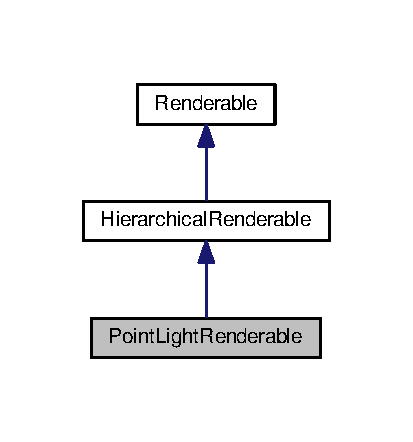
\includegraphics[width=198pt]{classPointLightRenderable__inherit__graph}
\end{center}
\end{figure}


Collaboration diagram for Point\+Light\+Renderable\+:\nopagebreak
\begin{figure}[H]
\begin{center}
\leavevmode
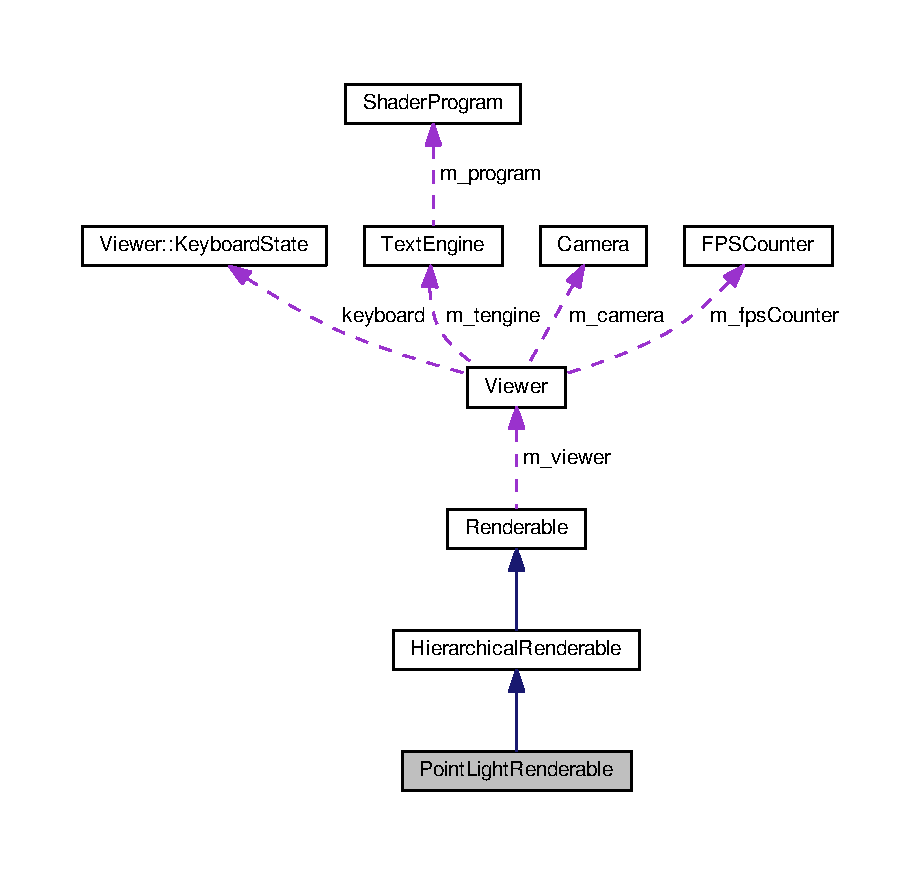
\includegraphics[width=350pt]{classPointLightRenderable__coll__graph}
\end{center}
\end{figure}
\subsection*{Public Member Functions}
\begin{DoxyCompactItemize}
\item 
\hyperlink{classPointLightRenderable_a7f981bb9210b5b50f982d5929eb1c27c}{$\sim$\+Point\+Light\+Renderable} ()
\item 
\hyperlink{classPointLightRenderable_a7eadc444c01d09bff0b612c4707b3c80}{Point\+Light\+Renderable} (\hyperlink{ShaderProgram_8hpp_af8e4af1ad4c53875ee5d32ab7e1f4966}{Shader\+Program\+Ptr} program, \hyperlink{Light_8hpp_a28898b9799350669037caef13c5115d2}{Point\+Light\+Ptr} light)
\end{DoxyCompactItemize}
\subsection*{Private Member Functions}
\begin{DoxyCompactItemize}
\item 
void \hyperlink{classPointLightRenderable_afdb8498c6af494231394d96a3f3f2315}{do\+\_\+draw} ()
\begin{DoxyCompactList}\small\item\em Draw virtual function. \end{DoxyCompactList}\item 
void \hyperlink{classPointLightRenderable_a5c4efe61c5061c739d3b68a7702f9df4}{do\+\_\+animate} (float time)
\begin{DoxyCompactList}\small\item\em Animate virtual function. \end{DoxyCompactList}\end{DoxyCompactItemize}
\subsection*{Private Attributes}
\begin{DoxyCompactItemize}
\item 
std\+::vector$<$ glm\+::vec3 $>$ \hyperlink{classPointLightRenderable_ae63fb46f04473b2c25c46e61744922aa}{m\+\_\+positions}
\item 
std\+::vector$<$ glm\+::vec4 $>$ \hyperlink{classPointLightRenderable_a6d45d8ebfe800a578f22a6cfa0b7981c}{m\+\_\+colors}
\item 
std\+::vector$<$ glm\+::vec3 $>$ \hyperlink{classPointLightRenderable_a91714162c3bed982468ba2e506430585}{m\+\_\+normals}
\item 
unsigned int \hyperlink{classPointLightRenderable_a013e5165f655d3a43144a4a16bcec001}{m\+\_\+p\+Buffer}
\item 
unsigned int \hyperlink{classPointLightRenderable_ab2f20160f2e541d4822ef4120c70dfc3}{m\+\_\+c\+Buffer}
\item 
unsigned int \hyperlink{classPointLightRenderable_af8c0b76df5c6f9470ffec65afea21b83}{m\+\_\+n\+Buffer}
\item 
\hyperlink{Light_8hpp_a28898b9799350669037caef13c5115d2}{Point\+Light\+Ptr} \hyperlink{classPointLightRenderable_a937b4cab5b786b27414374505769d1ce}{m\+\_\+light}
\end{DoxyCompactItemize}
\subsection*{Additional Inherited Members}


\subsection{Constructor \& Destructor Documentation}
\hypertarget{classPointLightRenderable_a7f981bb9210b5b50f982d5929eb1c27c}{\index{Point\+Light\+Renderable@{Point\+Light\+Renderable}!````~Point\+Light\+Renderable@{$\sim$\+Point\+Light\+Renderable}}
\index{````~Point\+Light\+Renderable@{$\sim$\+Point\+Light\+Renderable}!Point\+Light\+Renderable@{Point\+Light\+Renderable}}
\subsubsection[{$\sim$\+Point\+Light\+Renderable}]{\setlength{\rightskip}{0pt plus 5cm}Point\+Light\+Renderable\+::$\sim$\+Point\+Light\+Renderable (
\begin{DoxyParamCaption}
{}
\end{DoxyParamCaption}
)}}\label{classPointLightRenderable_a7f981bb9210b5b50f982d5929eb1c27c}
\hypertarget{classPointLightRenderable_a7eadc444c01d09bff0b612c4707b3c80}{\index{Point\+Light\+Renderable@{Point\+Light\+Renderable}!Point\+Light\+Renderable@{Point\+Light\+Renderable}}
\index{Point\+Light\+Renderable@{Point\+Light\+Renderable}!Point\+Light\+Renderable@{Point\+Light\+Renderable}}
\subsubsection[{Point\+Light\+Renderable}]{\setlength{\rightskip}{0pt plus 5cm}Point\+Light\+Renderable\+::\+Point\+Light\+Renderable (
\begin{DoxyParamCaption}
\item[{{\bf Shader\+Program\+Ptr}}]{program, }
\item[{{\bf Point\+Light\+Ptr}}]{light}
\end{DoxyParamCaption}
)}}\label{classPointLightRenderable_a7eadc444c01d09bff0b612c4707b3c80}


\subsection{Member Function Documentation}
\hypertarget{classPointLightRenderable_a5c4efe61c5061c739d3b68a7702f9df4}{\index{Point\+Light\+Renderable@{Point\+Light\+Renderable}!do\+\_\+animate@{do\+\_\+animate}}
\index{do\+\_\+animate@{do\+\_\+animate}!Point\+Light\+Renderable@{Point\+Light\+Renderable}}
\subsubsection[{do\+\_\+animate}]{\setlength{\rightskip}{0pt plus 5cm}void Point\+Light\+Renderable\+::do\+\_\+animate (
\begin{DoxyParamCaption}
\item[{float}]{time}
\end{DoxyParamCaption}
)\hspace{0.3cm}{\ttfamily [private]}, {\ttfamily [virtual]}}}\label{classPointLightRenderable_a5c4efe61c5061c739d3b68a7702f9df4}
Implementation to animate this renderable. 
\begin{DoxyParams}{Parameters}
{\em time} & The current simulation time. \\
\hline
\end{DoxyParams}


Implements \hyperlink{classRenderable_aa5206322555c9dece40b21e797629b34}{Renderable}.

\hypertarget{classPointLightRenderable_afdb8498c6af494231394d96a3f3f2315}{\index{Point\+Light\+Renderable@{Point\+Light\+Renderable}!do\+\_\+draw@{do\+\_\+draw}}
\index{do\+\_\+draw@{do\+\_\+draw}!Point\+Light\+Renderable@{Point\+Light\+Renderable}}
\subsubsection[{do\+\_\+draw}]{\setlength{\rightskip}{0pt plus 5cm}void Point\+Light\+Renderable\+::do\+\_\+draw (
\begin{DoxyParamCaption}
{}
\end{DoxyParamCaption}
)\hspace{0.3cm}{\ttfamily [private]}, {\ttfamily [virtual]}}}\label{classPointLightRenderable_afdb8498c6af494231394d96a3f3f2315}
Implementation to draw this renderable. 

Implements \hyperlink{classRenderable_a98ab6308c1d2b56dacda7c435fb38d5b}{Renderable}.



\subsection{Member Data Documentation}
\hypertarget{classPointLightRenderable_ab2f20160f2e541d4822ef4120c70dfc3}{\index{Point\+Light\+Renderable@{Point\+Light\+Renderable}!m\+\_\+c\+Buffer@{m\+\_\+c\+Buffer}}
\index{m\+\_\+c\+Buffer@{m\+\_\+c\+Buffer}!Point\+Light\+Renderable@{Point\+Light\+Renderable}}
\subsubsection[{m\+\_\+c\+Buffer}]{\setlength{\rightskip}{0pt plus 5cm}unsigned int Point\+Light\+Renderable\+::m\+\_\+c\+Buffer\hspace{0.3cm}{\ttfamily [private]}}}\label{classPointLightRenderable_ab2f20160f2e541d4822ef4120c70dfc3}
\hypertarget{classPointLightRenderable_a6d45d8ebfe800a578f22a6cfa0b7981c}{\index{Point\+Light\+Renderable@{Point\+Light\+Renderable}!m\+\_\+colors@{m\+\_\+colors}}
\index{m\+\_\+colors@{m\+\_\+colors}!Point\+Light\+Renderable@{Point\+Light\+Renderable}}
\subsubsection[{m\+\_\+colors}]{\setlength{\rightskip}{0pt plus 5cm}std\+::vector$<$ glm\+::vec4 $>$ Point\+Light\+Renderable\+::m\+\_\+colors\hspace{0.3cm}{\ttfamily [private]}}}\label{classPointLightRenderable_a6d45d8ebfe800a578f22a6cfa0b7981c}
\hypertarget{classPointLightRenderable_a937b4cab5b786b27414374505769d1ce}{\index{Point\+Light\+Renderable@{Point\+Light\+Renderable}!m\+\_\+light@{m\+\_\+light}}
\index{m\+\_\+light@{m\+\_\+light}!Point\+Light\+Renderable@{Point\+Light\+Renderable}}
\subsubsection[{m\+\_\+light}]{\setlength{\rightskip}{0pt plus 5cm}{\bf Point\+Light\+Ptr} Point\+Light\+Renderable\+::m\+\_\+light\hspace{0.3cm}{\ttfamily [private]}}}\label{classPointLightRenderable_a937b4cab5b786b27414374505769d1ce}
\hypertarget{classPointLightRenderable_af8c0b76df5c6f9470ffec65afea21b83}{\index{Point\+Light\+Renderable@{Point\+Light\+Renderable}!m\+\_\+n\+Buffer@{m\+\_\+n\+Buffer}}
\index{m\+\_\+n\+Buffer@{m\+\_\+n\+Buffer}!Point\+Light\+Renderable@{Point\+Light\+Renderable}}
\subsubsection[{m\+\_\+n\+Buffer}]{\setlength{\rightskip}{0pt plus 5cm}unsigned int Point\+Light\+Renderable\+::m\+\_\+n\+Buffer\hspace{0.3cm}{\ttfamily [private]}}}\label{classPointLightRenderable_af8c0b76df5c6f9470ffec65afea21b83}
\hypertarget{classPointLightRenderable_a91714162c3bed982468ba2e506430585}{\index{Point\+Light\+Renderable@{Point\+Light\+Renderable}!m\+\_\+normals@{m\+\_\+normals}}
\index{m\+\_\+normals@{m\+\_\+normals}!Point\+Light\+Renderable@{Point\+Light\+Renderable}}
\subsubsection[{m\+\_\+normals}]{\setlength{\rightskip}{0pt plus 5cm}std\+::vector$<$ glm\+::vec3 $>$ Point\+Light\+Renderable\+::m\+\_\+normals\hspace{0.3cm}{\ttfamily [private]}}}\label{classPointLightRenderable_a91714162c3bed982468ba2e506430585}
\hypertarget{classPointLightRenderable_a013e5165f655d3a43144a4a16bcec001}{\index{Point\+Light\+Renderable@{Point\+Light\+Renderable}!m\+\_\+p\+Buffer@{m\+\_\+p\+Buffer}}
\index{m\+\_\+p\+Buffer@{m\+\_\+p\+Buffer}!Point\+Light\+Renderable@{Point\+Light\+Renderable}}
\subsubsection[{m\+\_\+p\+Buffer}]{\setlength{\rightskip}{0pt plus 5cm}unsigned int Point\+Light\+Renderable\+::m\+\_\+p\+Buffer\hspace{0.3cm}{\ttfamily [private]}}}\label{classPointLightRenderable_a013e5165f655d3a43144a4a16bcec001}
\hypertarget{classPointLightRenderable_ae63fb46f04473b2c25c46e61744922aa}{\index{Point\+Light\+Renderable@{Point\+Light\+Renderable}!m\+\_\+positions@{m\+\_\+positions}}
\index{m\+\_\+positions@{m\+\_\+positions}!Point\+Light\+Renderable@{Point\+Light\+Renderable}}
\subsubsection[{m\+\_\+positions}]{\setlength{\rightskip}{0pt plus 5cm}std\+::vector$<$ glm\+::vec3 $>$ Point\+Light\+Renderable\+::m\+\_\+positions\hspace{0.3cm}{\ttfamily [private]}}}\label{classPointLightRenderable_ae63fb46f04473b2c25c46e61744922aa}


The documentation for this class was generated from the following file\+:\begin{DoxyCompactItemize}
\item 
/home/chardon/\+Depot/ensimag/2\+A\+\_\+\+G3\+D/practicals/teacher\+Source/include/lighting/\hyperlink{PointLightRenderable_8hpp}{Point\+Light\+Renderable.\+hpp}\end{DoxyCompactItemize}

\hypertarget{classQuadRenderable}{\section{Quad\+Renderable Class Reference}
\label{classQuadRenderable}\index{Quad\+Renderable@{Quad\+Renderable}}
}


Render a quad on the screen.  




{\ttfamily \#include $<$Quad\+Renderable.\+hpp$>$}



Inheritance diagram for Quad\+Renderable\+:\nopagebreak
\begin{figure}[H]
\begin{center}
\leavevmode
\includegraphics[width=198pt]{classQuadRenderable__inherit__graph}
\end{center}
\end{figure}


Collaboration diagram for Quad\+Renderable\+:\nopagebreak
\begin{figure}[H]
\begin{center}
\leavevmode
\includegraphics[width=350pt]{classQuadRenderable__coll__graph}
\end{center}
\end{figure}
\subsection*{Public Member Functions}
\begin{DoxyCompactItemize}
\item 
\hyperlink{classQuadRenderable_a188666a23247f2b8c37642f25856dc7f}{$\sim$\+Quad\+Renderable} ()
\item 
\hyperlink{classQuadRenderable_a3c4fc3b8118d06fc7e2457e76f2bc48a}{Quad\+Renderable} (\hyperlink{ShaderProgram_8hpp_af8e4af1ad4c53875ee5d32ab7e1f4966}{Shader\+Program\+Ptr} program, const glm\+::vec3 \&p1, const glm\+::vec3 \&p2, const glm\+::vec3 \&p3, const glm\+::vec3 \&p4, const glm\+::vec4 \&color=glm\+::vec4\{1.\+0, 0, 0, 1.\+0\})
\begin{DoxyCompactList}\small\item\em Build a quad passing by four vertices. \end{DoxyCompactList}\end{DoxyCompactItemize}
\subsection*{Private Member Functions}
\begin{DoxyCompactItemize}
\item 
void \hyperlink{classQuadRenderable_a584444dfbbb34ef5a6fac48a72aa51e6}{do\+\_\+draw} ()
\begin{DoxyCompactList}\small\item\em Draw virtual function. \end{DoxyCompactList}\item 
void \hyperlink{classQuadRenderable_a19fc1c1704e35cd89c31997e898fb9ba}{do\+\_\+animate} (float time)
\begin{DoxyCompactList}\small\item\em Animate virtual function. \end{DoxyCompactList}\end{DoxyCompactItemize}
\subsection*{Private Attributes}
\begin{DoxyCompactItemize}
\item 
std\+::vector$<$ glm\+::vec3 $>$ \hyperlink{classQuadRenderable_a98895c29eb360bfa5399856fd05808a3}{m\+\_\+positions}
\item 
std\+::vector$<$ glm\+::vec4 $>$ \hyperlink{classQuadRenderable_a775824ad790972ac1fb82553ce2d9268}{m\+\_\+colors}
\item 
std\+::vector$<$ glm\+::vec3 $>$ \hyperlink{classQuadRenderable_a6af0484f27f593537f05c7eb8386bd09}{m\+\_\+normals}
\item 
unsigned int \hyperlink{classQuadRenderable_a985335081fe25dd9556d86d6d168b5fe}{m\+\_\+p\+Buffer}
\item 
unsigned int \hyperlink{classQuadRenderable_af276accada410c35db3feb1456e6da15}{m\+\_\+c\+Buffer}
\item 
unsigned int \hyperlink{classQuadRenderable_aa812c4e6491db1ac7e464f5b3dc8561a}{m\+\_\+n\+Buffer}
\end{DoxyCompactItemize}
\subsection*{Additional Inherited Members}


\subsection{Detailed Description}
This class is used to render a quad on the screen. 

\subsection{Constructor \& Destructor Documentation}
\hypertarget{classQuadRenderable_a188666a23247f2b8c37642f25856dc7f}{\index{Quad\+Renderable@{Quad\+Renderable}!````~Quad\+Renderable@{$\sim$\+Quad\+Renderable}}
\index{````~Quad\+Renderable@{$\sim$\+Quad\+Renderable}!Quad\+Renderable@{Quad\+Renderable}}
\subsubsection[{$\sim$\+Quad\+Renderable}]{\setlength{\rightskip}{0pt plus 5cm}Quad\+Renderable\+::$\sim$\+Quad\+Renderable (
\begin{DoxyParamCaption}
{}
\end{DoxyParamCaption}
)}}\label{classQuadRenderable_a188666a23247f2b8c37642f25856dc7f}
\hypertarget{classQuadRenderable_a3c4fc3b8118d06fc7e2457e76f2bc48a}{\index{Quad\+Renderable@{Quad\+Renderable}!Quad\+Renderable@{Quad\+Renderable}}
\index{Quad\+Renderable@{Quad\+Renderable}!Quad\+Renderable@{Quad\+Renderable}}
\subsubsection[{Quad\+Renderable}]{\setlength{\rightskip}{0pt plus 5cm}Quad\+Renderable\+::\+Quad\+Renderable (
\begin{DoxyParamCaption}
\item[{{\bf Shader\+Program\+Ptr}}]{program, }
\item[{const glm\+::vec3 \&}]{p1, }
\item[{const glm\+::vec3 \&}]{p2, }
\item[{const glm\+::vec3 \&}]{p3, }
\item[{const glm\+::vec3 \&}]{p4, }
\item[{const glm\+::vec4 \&}]{color = {\ttfamily glm\+:\+:vec4\{1.0,~0,~0,~1.0\}}}
\end{DoxyParamCaption}
)}}\label{classQuadRenderable_a3c4fc3b8118d06fc7e2457e76f2bc48a}
Build a quad passing by four vertices. The quad is rendering thanks to two triangles\+: (p1, p2, p3) and (p1, p3, p4). 
\begin{DoxyParams}{Parameters}
{\em program} & Shader program used to render this quad. \\
\hline
{\em p1} & First quad vertex. \\
\hline
{\em p2} & Second quad vertex. \\
\hline
{\em p3} & Third quad vertex. \\
\hline
{\em p4} & Fourth quad vertex. \\
\hline
{\em color} & Color of the quad. \\
\hline
\end{DoxyParams}


\subsection{Member Function Documentation}
\hypertarget{classQuadRenderable_a19fc1c1704e35cd89c31997e898fb9ba}{\index{Quad\+Renderable@{Quad\+Renderable}!do\+\_\+animate@{do\+\_\+animate}}
\index{do\+\_\+animate@{do\+\_\+animate}!Quad\+Renderable@{Quad\+Renderable}}
\subsubsection[{do\+\_\+animate}]{\setlength{\rightskip}{0pt plus 5cm}void Quad\+Renderable\+::do\+\_\+animate (
\begin{DoxyParamCaption}
\item[{float}]{time}
\end{DoxyParamCaption}
)\hspace{0.3cm}{\ttfamily [private]}, {\ttfamily [virtual]}}}\label{classQuadRenderable_a19fc1c1704e35cd89c31997e898fb9ba}
Implementation to animate this renderable. 
\begin{DoxyParams}{Parameters}
{\em time} & The current simulation time. \\
\hline
\end{DoxyParams}


Implements \hyperlink{classRenderable_aa5206322555c9dece40b21e797629b34}{Renderable}.

\hypertarget{classQuadRenderable_a584444dfbbb34ef5a6fac48a72aa51e6}{\index{Quad\+Renderable@{Quad\+Renderable}!do\+\_\+draw@{do\+\_\+draw}}
\index{do\+\_\+draw@{do\+\_\+draw}!Quad\+Renderable@{Quad\+Renderable}}
\subsubsection[{do\+\_\+draw}]{\setlength{\rightskip}{0pt plus 5cm}void Quad\+Renderable\+::do\+\_\+draw (
\begin{DoxyParamCaption}
{}
\end{DoxyParamCaption}
)\hspace{0.3cm}{\ttfamily [private]}, {\ttfamily [virtual]}}}\label{classQuadRenderable_a584444dfbbb34ef5a6fac48a72aa51e6}
Implementation to draw this renderable. 

Implements \hyperlink{classRenderable_a98ab6308c1d2b56dacda7c435fb38d5b}{Renderable}.



\subsection{Member Data Documentation}
\hypertarget{classQuadRenderable_af276accada410c35db3feb1456e6da15}{\index{Quad\+Renderable@{Quad\+Renderable}!m\+\_\+c\+Buffer@{m\+\_\+c\+Buffer}}
\index{m\+\_\+c\+Buffer@{m\+\_\+c\+Buffer}!Quad\+Renderable@{Quad\+Renderable}}
\subsubsection[{m\+\_\+c\+Buffer}]{\setlength{\rightskip}{0pt plus 5cm}unsigned int Quad\+Renderable\+::m\+\_\+c\+Buffer\hspace{0.3cm}{\ttfamily [private]}}}\label{classQuadRenderable_af276accada410c35db3feb1456e6da15}
\hypertarget{classQuadRenderable_a775824ad790972ac1fb82553ce2d9268}{\index{Quad\+Renderable@{Quad\+Renderable}!m\+\_\+colors@{m\+\_\+colors}}
\index{m\+\_\+colors@{m\+\_\+colors}!Quad\+Renderable@{Quad\+Renderable}}
\subsubsection[{m\+\_\+colors}]{\setlength{\rightskip}{0pt plus 5cm}std\+::vector$<$ glm\+::vec4 $>$ Quad\+Renderable\+::m\+\_\+colors\hspace{0.3cm}{\ttfamily [private]}}}\label{classQuadRenderable_a775824ad790972ac1fb82553ce2d9268}
\hypertarget{classQuadRenderable_aa812c4e6491db1ac7e464f5b3dc8561a}{\index{Quad\+Renderable@{Quad\+Renderable}!m\+\_\+n\+Buffer@{m\+\_\+n\+Buffer}}
\index{m\+\_\+n\+Buffer@{m\+\_\+n\+Buffer}!Quad\+Renderable@{Quad\+Renderable}}
\subsubsection[{m\+\_\+n\+Buffer}]{\setlength{\rightskip}{0pt plus 5cm}unsigned int Quad\+Renderable\+::m\+\_\+n\+Buffer\hspace{0.3cm}{\ttfamily [private]}}}\label{classQuadRenderable_aa812c4e6491db1ac7e464f5b3dc8561a}
\hypertarget{classQuadRenderable_a6af0484f27f593537f05c7eb8386bd09}{\index{Quad\+Renderable@{Quad\+Renderable}!m\+\_\+normals@{m\+\_\+normals}}
\index{m\+\_\+normals@{m\+\_\+normals}!Quad\+Renderable@{Quad\+Renderable}}
\subsubsection[{m\+\_\+normals}]{\setlength{\rightskip}{0pt plus 5cm}std\+::vector$<$ glm\+::vec3 $>$ Quad\+Renderable\+::m\+\_\+normals\hspace{0.3cm}{\ttfamily [private]}}}\label{classQuadRenderable_a6af0484f27f593537f05c7eb8386bd09}
\hypertarget{classQuadRenderable_a985335081fe25dd9556d86d6d168b5fe}{\index{Quad\+Renderable@{Quad\+Renderable}!m\+\_\+p\+Buffer@{m\+\_\+p\+Buffer}}
\index{m\+\_\+p\+Buffer@{m\+\_\+p\+Buffer}!Quad\+Renderable@{Quad\+Renderable}}
\subsubsection[{m\+\_\+p\+Buffer}]{\setlength{\rightskip}{0pt plus 5cm}unsigned int Quad\+Renderable\+::m\+\_\+p\+Buffer\hspace{0.3cm}{\ttfamily [private]}}}\label{classQuadRenderable_a985335081fe25dd9556d86d6d168b5fe}
\hypertarget{classQuadRenderable_a98895c29eb360bfa5399856fd05808a3}{\index{Quad\+Renderable@{Quad\+Renderable}!m\+\_\+positions@{m\+\_\+positions}}
\index{m\+\_\+positions@{m\+\_\+positions}!Quad\+Renderable@{Quad\+Renderable}}
\subsubsection[{m\+\_\+positions}]{\setlength{\rightskip}{0pt plus 5cm}std\+::vector$<$ glm\+::vec3 $>$ Quad\+Renderable\+::m\+\_\+positions\hspace{0.3cm}{\ttfamily [private]}}}\label{classQuadRenderable_a98895c29eb360bfa5399856fd05808a3}


The documentation for this class was generated from the following file\+:\begin{DoxyCompactItemize}
\item 
/home/chardon/\+Depot/ensimag/2\+A\+\_\+\+G3\+D/practicals/teacher\+Source/include/\hyperlink{QuadRenderable_8hpp}{Quad\+Renderable.\+hpp}\end{DoxyCompactItemize}

\hypertarget{classRenderable}{\section{Renderable Class Reference}
\label{classRenderable}\index{Renderable@{Renderable}}
}


\hyperlink{classRenderable}{Renderable} interface.  




{\ttfamily \#include $<$Renderable.\+hpp$>$}



Inheritance diagram for Renderable\+:\nopagebreak
\begin{figure}[H]
\begin{center}
\leavevmode
\includegraphics[height=550pt]{classRenderable__inherit__graph}
\end{center}
\end{figure}


Collaboration diagram for Renderable\+:\nopagebreak
\begin{figure}[H]
\begin{center}
\leavevmode
\includegraphics[width=350pt]{classRenderable__coll__graph}
\end{center}
\end{figure}
\subsection*{Public Member Functions}
\begin{Indent}{\bf Construction/\+Destruction of renderable instances.}\par
\begin{DoxyCompactItemize}
\item 
virtual \hyperlink{classRenderable_a4c9e03ac345df99a010c2ad9f8632af2}{$\sim$\+Renderable} ()
\begin{DoxyCompactList}\small\item\em Destructor. \end{DoxyCompactList}\item 
\hyperlink{classRenderable_ae02271675fa76ef56e7e3b8b26d1efb0}{Renderable} (\hyperlink{ShaderProgram_8hpp_af8e4af1ad4c53875ee5d32ab7e1f4966}{Shader\+Program\+Ptr} program)
\begin{DoxyCompactList}\small\item\em \hyperlink{classRenderable}{Renderable} program constructor. \end{DoxyCompactList}\end{DoxyCompactItemize}
\end{Indent}
\begin{Indent}{\bf Public interface}\par
\begin{DoxyCompactItemize}
\item 
void \hyperlink{classRenderable_a70d8b63cc49efc0327bbb119c521dcef}{set\+Model\+Matrix} (const glm\+::mat4 \&model)
\begin{DoxyCompactList}\small\item\em Set the model matrix. \end{DoxyCompactList}\item 
const glm\+::mat4 \& \hyperlink{classRenderable_ab4e9182825d81d3bf3d3822bc26c4714}{get\+Model\+Matrix} () const 
\begin{DoxyCompactList}\small\item\em Get the model matrix. \end{DoxyCompactList}\item 
void \hyperlink{classRenderable_a58242b044ba6359e4d89ed284b96906c}{set\+Shader\+Program} (\hyperlink{ShaderProgram_8hpp_af8e4af1ad4c53875ee5d32ab7e1f4966}{Shader\+Program\+Ptr} prog)
\begin{DoxyCompactList}\small\item\em Change the shader program. \end{DoxyCompactList}\end{DoxyCompactItemize}
\end{Indent}
\begin{Indent}{\bf Public interface used by Viewer.}\par
{\em Those functions are automatically called by the \hyperlink{classViewer}{Viewer} on added \hyperlink{classRenderable}{Renderable}. You are not expected to call them directly. }\begin{DoxyCompactItemize}
\item 
void \hyperlink{classRenderable_aaa73d54539b1b84d5b3e12293d7b3610}{bind\+Shader\+Program} ()
\begin{DoxyCompactList}\small\item\em Bind the shader program on the G\+P\+U. \end{DoxyCompactList}\item 
void \hyperlink{classRenderable_a1d3d81445852e84244bc6f5c3f078292}{unbind\+Shader\+Program} ()
\begin{DoxyCompactList}\small\item\em Unbind the shader program of the G\+P\+U. \end{DoxyCompactList}\item 
int \hyperlink{classRenderable_a905c76682e391c2aed94f021447bf63d}{projection\+Location} ()
\begin{DoxyCompactList}\small\item\em Get the location of the projection matrix in the shader program. \end{DoxyCompactList}\item 
int \hyperlink{classRenderable_a3e7c969092e6e42d30fec9dfa6ba988a}{view\+Location} ()
\begin{DoxyCompactList}\small\item\em Get the location of the view matrix in the shader program. \end{DoxyCompactList}\item 
void \hyperlink{classRenderable_a0d371901a19b8cfe50b76b842adba70a}{draw} ()
\begin{DoxyCompactList}\small\item\em Draw this renderable. \end{DoxyCompactList}\item 
virtual void \hyperlink{classRenderable_a74fd37d6852fb727e1a5fe72541d269d}{animate} (float time)
\begin{DoxyCompactList}\small\item\em Animate this renderable. \end{DoxyCompactList}\item 
void \hyperlink{classRenderable_a02e29d97fae52b6240ffb43ac5fb82de}{key\+Pressed\+Event} (sf\+::\+Event \&e)
\begin{DoxyCompactList}\small\item\em Handle a key pressed event. \end{DoxyCompactList}\item 
void \hyperlink{classRenderable_a07d0883e8566fa86d224b4d281b373b3}{key\+Released\+Event} (sf\+::\+Event \&e)
\begin{DoxyCompactList}\small\item\em Handle a key released event. \end{DoxyCompactList}\item 
void \hyperlink{classRenderable_a2cc5c2d8476a762be1b0d47425c1149b}{mouse\+Press\+Event} (sf\+::\+Event \&e)
\begin{DoxyCompactList}\small\item\em Handle a mouse pressed event. \end{DoxyCompactList}\item 
void \hyperlink{classRenderable_a1a9c0d11946d3708462b8b4a364ac0d3}{mouse\+Release\+Event} (sf\+::\+Event \&e)
\begin{DoxyCompactList}\small\item\em Handle a mouse released event. \end{DoxyCompactList}\item 
void \hyperlink{classRenderable_a3ee244b2ff6682fb4b4b11b92819c2a2}{mouse\+Wheel\+Event} (sf\+::\+Event \&e)
\begin{DoxyCompactList}\small\item\em Handle a mouse wheel event. \end{DoxyCompactList}\item 
void \hyperlink{classRenderable_aabf21b5d1b75aed4c4f4b9466d658caa}{mouse\+Move\+Event} (sf\+::\+Event \&e)
\begin{DoxyCompactList}\small\item\em Handle a mouse move event. \end{DoxyCompactList}\item 
\hyperlink{ShaderProgram_8hpp_af8e4af1ad4c53875ee5d32ab7e1f4966}{Shader\+Program\+Ptr} \hyperlink{classRenderable_ad6bb136447d0d5968345724d3381714a}{get\+Shader\+Program} () const 
\end{DoxyCompactItemize}
\end{Indent}
\subsection*{Protected Attributes}
\begin{Indent}{\bf Protected members.}\par
{\em We want those members to be accessible in the derived classes. }\begin{DoxyCompactItemize}
\item 
glm\+::mat4 \hyperlink{classRenderable_ab3a7f6112bd9d8c37ab10dac24186b25}{m\+\_\+model}
\item 
\hyperlink{ShaderProgram_8hpp_af8e4af1ad4c53875ee5d32ab7e1f4966}{Shader\+Program\+Ptr} \hyperlink{classRenderable_ad4004cea2d9ca6cc91eb03b4ce885088}{m\+\_\+shader\+Program}
\item 
friend \hyperlink{classRenderable_aaf644a3bff63df86024c9ad960d00e74}{Viewer}
\item 
\hyperlink{classViewer}{Viewer} $\ast$ \hyperlink{classRenderable_a691422fa44ec05fae13d94902870d6c0}{m\+\_\+viewer}
\end{DoxyCompactItemize}
\end{Indent}
\subsection*{Private Member Functions}
\begin{Indent}{\bf Private viewer interface.}\par
{\em According to guideline \#1, we have used the Template method. Now we are using guideline \#2 for virtual methods. }\begin{DoxyCompactItemize}
\item 
virtual void \hyperlink{classRenderable_a98ab6308c1d2b56dacda7c435fb38d5b}{do\+\_\+draw} ()=0
\begin{DoxyCompactList}\small\item\em Draw virtual function. \end{DoxyCompactList}\item 
virtual void \hyperlink{classRenderable_aa5206322555c9dece40b21e797629b34}{do\+\_\+animate} (float time)=0
\begin{DoxyCompactList}\small\item\em Animate virtual function. \end{DoxyCompactList}\item 
virtual void \hyperlink{classRenderable_a49e39be950dca7a925b8b79c13241e6b}{do\+\_\+key\+Pressed\+Event} (sf\+::\+Event \&e)
\begin{DoxyCompactList}\small\item\em Handle a key pressed event. \end{DoxyCompactList}\item 
virtual void \hyperlink{classRenderable_a89d4bacd849c3606529f92c44b0a3bc1}{do\+\_\+key\+Released\+Event} (sf\+::\+Event \&e)
\begin{DoxyCompactList}\small\item\em Handle a key released event. \end{DoxyCompactList}\item 
virtual void \hyperlink{classRenderable_a9de3c5f272bbeeb32151056df9384309}{do\+\_\+mouse\+Press\+Event} (sf\+::\+Event \&e)
\begin{DoxyCompactList}\small\item\em Handle a mouse pressed event. \end{DoxyCompactList}\item 
virtual void \hyperlink{classRenderable_adae67d88a7803f445f4d8b81a56cec60}{do\+\_\+mouse\+Release\+Event} (sf\+::\+Event \&e)
\begin{DoxyCompactList}\small\item\em Handle a mouse released event. \end{DoxyCompactList}\item 
virtual void \hyperlink{classRenderable_ab0d2c0b1171e5c593918fc39cd7fec19}{do\+\_\+mouse\+Wheel\+Event} (sf\+::\+Event \&e)
\begin{DoxyCompactList}\small\item\em Handle a mouse wheel event. \end{DoxyCompactList}\item 
virtual void \hyperlink{classRenderable_a4e7d850da9dd8ad9ef5693dadd4001d2}{do\+\_\+mouse\+Move\+Event} (sf\+::\+Event \&e)
\begin{DoxyCompactList}\small\item\em Handle a mouse move event. \end{DoxyCompactList}\end{DoxyCompactItemize}
\end{Indent}
\begin{Indent}{\bf Private interface for Renderable sub classes.}\par
{\em Those functions are meant to be overridden in subclassed of \hyperlink{classRenderable}{Renderable}, in order to have additional operations done before and after drawing and animating. \begin{DoxySeeAlso}{See also}
\hyperlink{classHierarchicalRenderable}{Hierarchical\+Renderable}. 
\end{DoxySeeAlso}
}\begin{DoxyCompactItemize}
\item 
virtual void \hyperlink{classRenderable_ad2fd96564194f598555b4f141e8c48be}{before\+Draw} ()
\begin{DoxyCompactList}\small\item\em Perform operation before drawing a renderable. \end{DoxyCompactList}\item 
virtual void \hyperlink{classRenderable_a9c715cafdda260b94bf6fe12853a3bb7}{after\+Draw} ()
\begin{DoxyCompactList}\small\item\em Perform operation after drawing a renderable. \end{DoxyCompactList}\item 
virtual void \hyperlink{classRenderable_a8eea615c4abdd96d6747afab8e0c7a95}{before\+Animate} (float time)
\begin{DoxyCompactList}\small\item\em Perform operation before animating a renderable. \end{DoxyCompactList}\item 
virtual void \hyperlink{classRenderable_a027e4c23636f492df33461a23320a336}{after\+Animate} (float time)
\begin{DoxyCompactList}\small\item\em Perform operation after animating a renderable. \end{DoxyCompactList}\item 
\hyperlink{classViewer}{Viewer} $\ast$ \hyperlink{classRenderable_aa7e8cdb8786681b77ee454b5ebe00483}{get\+Viewer} () const 
\end{DoxyCompactItemize}
\end{Indent}


\subsection{Detailed Description}
A renderable is a concept often used in graphic applications. It can wear many names, such as drawable in the Android Framework \href{http://developer.android.com/guide/topics/resources/drawable-resource.html}{\tt http\+://developer.\+android.\+com/guide/topics/resources/drawable-\/resource.\+html} and in the S\+F\+M\+L library \href{http://www.sfml-dev.org/documentation/2.0/classsf_1_1Drawable.php,}{\tt http\+://www.\+sfml-\/dev.\+org/documentation/2.\+0/classsf\+\_\+1\+\_\+1\+Drawable.\+php,} or \hyperlink{classRenderable}{Renderable} in the O\+G\+R\+E Engine \href{http://www.ogre3d.org/docs/api/1.9/class_ogre_1_1_renderable.html}{\tt http\+://www.\+ogre3d.\+org/docs/api/1.\+9/class\+\_\+ogre\+\_\+1\+\_\+1\+\_\+renderable.\+html}. There are other commonly used concepts such as animable. Instead of building a wide hierarchy of concepts, we chose to merge all the necessary concepts of the objects that will compose our scenes into the \hyperlink{classRenderable}{Renderable} class.

This class is an interface we need to implement to create 3\+D objects. In particular, we must define the pure virtual member functions \hyperlink{classRenderable_a98ab6308c1d2b56dacda7c435fb38d5b}{do\+\_\+draw()} and \hyperlink{classRenderable_aa5206322555c9dece40b21e797629b34}{do\+\_\+animate( float time )}. The \hyperlink{classViewer}{Viewer} class can handle any non abstract derived class to display it for you, animate it or to send interaction events to it.

If you want the \hyperlink{classViewer}{Viewer} managing your renderables to automatically set the view and the projection matrices for you, remember to name the corresponding uniform matrices as follow in your shaders\+:
\begin{DoxyItemize}
\item {\ttfamily mat4} {\ttfamily view\+Mat}, for the view matrix
\item {\ttfamily mat4} {\ttfamily proj\+Mat}, for the projection matrix
\end{DoxyItemize}

\begin{DoxyNote}{Note}
As this class use virtuality, here are some words about the subject to ease your learning of c++ as well as learning computer graphics. This note is taken from a nice article available at \href{http://www.gotw.ca/publications/mill18.htm}{\tt http\+://www.\+gotw.\+ca/publications/mill18.\+htm}. Prefer to make base class virtual functions private (or protected if you really must). This separates the concerns of interface and implementation, which stabilizes interfaces and makes implementation decisions easier to change and refactor later. Here are some guidelines\+: \begin{DoxyItemize}
\item \#1 Prefer to make interfaces nonvirtual, using Template Method. \item \#2 Prefer to make virtual functions private. \item \#3 Only if derived classes need to invoke the base implementation of a virtual function, make the virtual function protected. \item \#4 A base class destructor should be either public and virtual, or protected and nonvirtual. In the first case, you can do something like {\ttfamily  delete base\+Ptr}, while in the second case, you can not.\end{DoxyItemize}

\end{DoxyNote}
\begin{DoxySeeAlso}{See also}
\hyperlink{classHierarchicalRenderable}{Hierarchical\+Renderable} 
\end{DoxySeeAlso}


\subsection{Constructor \& Destructor Documentation}
\hypertarget{classRenderable_a4c9e03ac345df99a010c2ad9f8632af2}{\index{Renderable@{Renderable}!````~Renderable@{$\sim$\+Renderable}}
\index{````~Renderable@{$\sim$\+Renderable}!Renderable@{Renderable}}
\subsubsection[{$\sim$\+Renderable}]{\setlength{\rightskip}{0pt plus 5cm}virtual Renderable\+::$\sim$\+Renderable (
\begin{DoxyParamCaption}
{}
\end{DoxyParamCaption}
)\hspace{0.3cm}{\ttfamily [virtual]}}}\label{classRenderable_a4c9e03ac345df99a010c2ad9f8632af2}
Some smart pointers to this base class could be stored, such as in \hyperlink{classViewer}{Viewer}. As such, the destructor needs to be public and virtual (guideline \#4). \hypertarget{classRenderable_ae02271675fa76ef56e7e3b8b26d1efb0}{\index{Renderable@{Renderable}!Renderable@{Renderable}}
\index{Renderable@{Renderable}!Renderable@{Renderable}}
\subsubsection[{Renderable}]{\setlength{\rightskip}{0pt plus 5cm}Renderable\+::\+Renderable (
\begin{DoxyParamCaption}
\item[{{\bf Shader\+Program\+Ptr}}]{program}
\end{DoxyParamCaption}
)}}\label{classRenderable_ae02271675fa76ef56e7e3b8b26d1efb0}
Initialize the model matrix \hyperlink{classRenderable_ab3a7f6112bd9d8c37ab10dac24186b25}{m\+\_\+model} to identity. Set the shader program \hyperlink{classRenderable_ad4004cea2d9ca6cc91eb03b4ce885088}{m\+\_\+shader\+Program} to {\itshape program}. 
\begin{DoxyParams}{Parameters}
{\em program} & Shader program to use to draw this. \\
\hline
\end{DoxyParams}
\begin{DoxySeeAlso}{See also}
\hyperlink{classShaderProgram}{Shader\+Program} 
\end{DoxySeeAlso}


\subsection{Member Function Documentation}
\hypertarget{classRenderable_a027e4c23636f492df33461a23320a336}{\index{Renderable@{Renderable}!after\+Animate@{after\+Animate}}
\index{after\+Animate@{after\+Animate}!Renderable@{Renderable}}
\subsubsection[{after\+Animate}]{\setlength{\rightskip}{0pt plus 5cm}virtual void Renderable\+::after\+Animate (
\begin{DoxyParamCaption}
\item[{float}]{time}
\end{DoxyParamCaption}
)\hspace{0.3cm}{\ttfamily [private]}, {\ttfamily [virtual]}}}\label{classRenderable_a027e4c23636f492df33461a23320a336}
Override this function to perform additional operations after calling \hyperlink{classRenderable_aa5206322555c9dece40b21e797629b34}{do\+\_\+animate()} of the concrete renderable class. 
\begin{DoxyParams}{Parameters}
{\em time} & The current simulation time. \\
\hline
\end{DoxyParams}


Reimplemented in \hyperlink{classHierarchicalRenderable_a8de5020d6678c97050079150bcb131fa}{Hierarchical\+Renderable}.

\hypertarget{classRenderable_a9c715cafdda260b94bf6fe12853a3bb7}{\index{Renderable@{Renderable}!after\+Draw@{after\+Draw}}
\index{after\+Draw@{after\+Draw}!Renderable@{Renderable}}
\subsubsection[{after\+Draw}]{\setlength{\rightskip}{0pt plus 5cm}virtual void Renderable\+::after\+Draw (
\begin{DoxyParamCaption}
{}
\end{DoxyParamCaption}
)\hspace{0.3cm}{\ttfamily [private]}, {\ttfamily [virtual]}}}\label{classRenderable_a9c715cafdda260b94bf6fe12853a3bb7}
Override this function to perform additional operations after calling \hyperlink{classRenderable_a98ab6308c1d2b56dacda7c435fb38d5b}{do\+\_\+draw()} of the concrete renderable class. 

Reimplemented in \hyperlink{classHierarchicalRenderable_a50fa8b46938a3da839829523838ddf2c}{Hierarchical\+Renderable}.

\hypertarget{classRenderable_a74fd37d6852fb727e1a5fe72541d269d}{\index{Renderable@{Renderable}!animate@{animate}}
\index{animate@{animate}!Renderable@{Renderable}}
\subsubsection[{animate}]{\setlength{\rightskip}{0pt plus 5cm}virtual void Renderable\+::animate (
\begin{DoxyParamCaption}
\item[{float}]{time}
\end{DoxyParamCaption}
)\hspace{0.3cm}{\ttfamily [virtual]}}}\label{classRenderable_a74fd37d6852fb727e1a5fe72541d269d}
This function calls the private pure virtual function {\ttfamily  do\+\_\+animate(time) } (guidelines \#1 and \#2). The simulation time equals zero when the animation is started (see \hyperlink{classViewer_a912259c3206eed1ebc1d24f7425e99cd}{Viewer\+::start\+Animation()}). 
\begin{DoxyParams}{Parameters}
{\em time} & Current simulation time. \\
\hline
\end{DoxyParams}
\hypertarget{classRenderable_a8eea615c4abdd96d6747afab8e0c7a95}{\index{Renderable@{Renderable}!before\+Animate@{before\+Animate}}
\index{before\+Animate@{before\+Animate}!Renderable@{Renderable}}
\subsubsection[{before\+Animate}]{\setlength{\rightskip}{0pt plus 5cm}virtual void Renderable\+::before\+Animate (
\begin{DoxyParamCaption}
\item[{float}]{time}
\end{DoxyParamCaption}
)\hspace{0.3cm}{\ttfamily [private]}, {\ttfamily [virtual]}}}\label{classRenderable_a8eea615c4abdd96d6747afab8e0c7a95}
Override this function to perform additional operations before calling \hyperlink{classRenderable_aa5206322555c9dece40b21e797629b34}{do\+\_\+animate()} of the concrete renderable class. 
\begin{DoxyParams}{Parameters}
{\em time} & The current simulation time. \\
\hline
\end{DoxyParams}
\hypertarget{classRenderable_ad2fd96564194f598555b4f141e8c48be}{\index{Renderable@{Renderable}!before\+Draw@{before\+Draw}}
\index{before\+Draw@{before\+Draw}!Renderable@{Renderable}}
\subsubsection[{before\+Draw}]{\setlength{\rightskip}{0pt plus 5cm}virtual void Renderable\+::before\+Draw (
\begin{DoxyParamCaption}
{}
\end{DoxyParamCaption}
)\hspace{0.3cm}{\ttfamily [private]}, {\ttfamily [virtual]}}}\label{classRenderable_ad2fd96564194f598555b4f141e8c48be}
Override this function to perform additional operations before calling \hyperlink{classRenderable_a98ab6308c1d2b56dacda7c435fb38d5b}{do\+\_\+draw()} of the concrete renderable class. 

Reimplemented in \hyperlink{classHierarchicalRenderable_aedbaa13858872d5dcd7ce644da9a66e1}{Hierarchical\+Renderable}.

\hypertarget{classRenderable_aaa73d54539b1b84d5b3e12293d7b3610}{\index{Renderable@{Renderable}!bind\+Shader\+Program@{bind\+Shader\+Program}}
\index{bind\+Shader\+Program@{bind\+Shader\+Program}!Renderable@{Renderable}}
\subsubsection[{bind\+Shader\+Program}]{\setlength{\rightskip}{0pt plus 5cm}void Renderable\+::bind\+Shader\+Program (
\begin{DoxyParamCaption}
{}
\end{DoxyParamCaption}
)}}\label{classRenderable_aaa73d54539b1b84d5b3e12293d7b3610}
Modify the Open\+G\+L state such that the next drawing command use the program shader of this renderable to render the primitives. \hypertarget{classRenderable_aa5206322555c9dece40b21e797629b34}{\index{Renderable@{Renderable}!do\+\_\+animate@{do\+\_\+animate}}
\index{do\+\_\+animate@{do\+\_\+animate}!Renderable@{Renderable}}
\subsubsection[{do\+\_\+animate}]{\setlength{\rightskip}{0pt plus 5cm}virtual void Renderable\+::do\+\_\+animate (
\begin{DoxyParamCaption}
\item[{float}]{time}
\end{DoxyParamCaption}
)\hspace{0.3cm}{\ttfamily [private]}, {\ttfamily [pure virtual]}}}\label{classRenderable_aa5206322555c9dece40b21e797629b34}
Implementation to animate this renderable. 
\begin{DoxyParams}{Parameters}
{\em time} & The current simulation time. \\
\hline
\end{DoxyParams}


Implemented in \hyperlink{classControlledForceFieldRenderable_a3ab6b5efaa5d5b988d92c4fee3e770a0}{Controlled\+Force\+Field\+Renderable}, \hyperlink{classFrameRenderable_a331b31de3a4988acf6304c30762d99cc}{Frame\+Renderable}, \hyperlink{classDynamicSystemRenderable_acd30af04cdca7cdc68ae2d49c179d2dc}{Dynamic\+System\+Renderable}, \hyperlink{classKeyframedCylinderRenderable_a59d9e6dedbf2e4105c08a8b6516cdd56}{Keyframed\+Cylinder\+Renderable}, \hyperlink{classQuadRenderable_a19fc1c1704e35cd89c31997e898fb9ba}{Quad\+Renderable}, \hyperlink{classParticleListRenderable_a25adb6020cb86abb50d33d76a5cde1f1}{Particle\+List\+Renderable}, \hyperlink{classBillboardRenderable_a99db8d2221571aed576e2f1e56ddc00e}{Billboard\+Renderable}, \hyperlink{classSpringListRenderable_a32460ca63254ddaf716697b8402c8a37}{Spring\+List\+Renderable}, \hyperlink{classParticleRenderable_a8c4e33166ba0e4ee4cf1985eedea5aa3}{Particle\+Renderable}, \hyperlink{classSpringForceFieldRenderable_a7ddf9b99051f6a3bd0c4d1f215f4c2b6}{Spring\+Force\+Field\+Renderable}, \hyperlink{classConstantForceFieldRenderable_aa2c53dcf6411244d5a5e4ed562f9574c}{Constant\+Force\+Field\+Renderable}, \hyperlink{classTexturedPlaneRenderable_a945edb4f74583f73813821bfcecbda0f}{Textured\+Plane\+Renderable}, \hyperlink{classLightedMeshRenderable_aa22c64fe3f33f88c164ffa087c9ec71f}{Lighted\+Mesh\+Renderable}, \hyperlink{classDirectionalLightRenderable_a7caf2f55742229944de3f6a9ee3f27ac}{Directional\+Light\+Renderable}, \hyperlink{classMipMapCubeRenderable_a24b35ddfe3681e641db25ed3dd46fda6}{Mip\+Map\+Cube\+Renderable}, \hyperlink{classMultiTexturedCubeRenderable_a1db1e5f6c10f62874aef22e346906979}{Multi\+Textured\+Cube\+Renderable}, \hyperlink{classLightedCylinderRenderable_a7ecf5b614bf6e98335e9b46edfc64e67}{Lighted\+Cylinder\+Renderable}, \hyperlink{classTexturedCubeRenderable_a8c48dedcd36a690591de101e2288cb0a}{Textured\+Cube\+Renderable}, \hyperlink{classHierarchicalMeshRenderable_a291689e73c0d7d2e733c587cd0062747}{Hierarchical\+Mesh\+Renderable}, \hyperlink{classLightedCubeRenderable_a2888876e6b826899dfe0611c0021b161}{Lighted\+Cube\+Renderable}, \hyperlink{classPointLightRenderable_a5c4efe61c5061c739d3b68a7702f9df4}{Point\+Light\+Renderable}, \hyperlink{classSpotLightRenderable_a628c20078ed7f102927e5d36fe25bb57}{Spot\+Light\+Renderable}, \hyperlink{classHierarchicalCylinderRenderable_a151ed55445a3bbbabdc9d19231a64a52}{Hierarchical\+Cylinder\+Renderable}, and \hyperlink{classHierarchicalSphereRenderable_a712e4865f38fced13bc3aa5be7a17764}{Hierarchical\+Sphere\+Renderable}.

\hypertarget{classRenderable_a98ab6308c1d2b56dacda7c435fb38d5b}{\index{Renderable@{Renderable}!do\+\_\+draw@{do\+\_\+draw}}
\index{do\+\_\+draw@{do\+\_\+draw}!Renderable@{Renderable}}
\subsubsection[{do\+\_\+draw}]{\setlength{\rightskip}{0pt plus 5cm}virtual void Renderable\+::do\+\_\+draw (
\begin{DoxyParamCaption}
{}
\end{DoxyParamCaption}
)\hspace{0.3cm}{\ttfamily [private]}, {\ttfamily [pure virtual]}}}\label{classRenderable_a98ab6308c1d2b56dacda7c435fb38d5b}
Implementation to draw this renderable. 

Implemented in \hyperlink{classControlledForceFieldRenderable_a5b73eb28c70b0a37ce4f69ec6a63823a}{Controlled\+Force\+Field\+Renderable}, \hyperlink{classFrameRenderable_aafa6b6444c8fa20a177eb562ba1a2672}{Frame\+Renderable}, \hyperlink{classDynamicSystemRenderable_a8064176726a5d4b857a5e6a0fc73ff29}{Dynamic\+System\+Renderable}, \hyperlink{classKeyframedCylinderRenderable_abbfc6deaafd95aa58feb2c08b22d1050}{Keyframed\+Cylinder\+Renderable}, \hyperlink{classQuadRenderable_a584444dfbbb34ef5a6fac48a72aa51e6}{Quad\+Renderable}, \hyperlink{classParticleListRenderable_af34f9d0c377aa749e52d226d9cf49d89}{Particle\+List\+Renderable}, \hyperlink{classBillboardRenderable_af3c5c220c558b0902acbbb5dd3f81174}{Billboard\+Renderable}, \hyperlink{classSpringListRenderable_a3188f3904567441c4578ebbbc1d4db92}{Spring\+List\+Renderable}, \hyperlink{classParticleRenderable_a1313290984b718988098504838fd4ee9}{Particle\+Renderable}, \hyperlink{classSpringForceFieldRenderable_ad74386934bac1b650a973abeed2a9a33}{Spring\+Force\+Field\+Renderable}, \hyperlink{classConstantForceFieldRenderable_af9ee973e392967a5da31b0b9b67d3fdd}{Constant\+Force\+Field\+Renderable}, \hyperlink{classTexturedPlaneRenderable_ab81503b6d91dc3b3a16f774197a14438}{Textured\+Plane\+Renderable}, \hyperlink{classLightedMeshRenderable_a7e4e538e3f45818789f28924fd18a478}{Lighted\+Mesh\+Renderable}, \hyperlink{classDirectionalLightRenderable_a9560a1e6c2b525de69140ab0d8059734}{Directional\+Light\+Renderable}, \hyperlink{classMipMapCubeRenderable_a739176af783a8cb15239d86b723f9882}{Mip\+Map\+Cube\+Renderable}, \hyperlink{classMultiTexturedCubeRenderable_a3dafc49b8a8b6b5f9ed2928c91c2cd6f}{Multi\+Textured\+Cube\+Renderable}, \hyperlink{classLightedCylinderRenderable_a327da1ffb8ac46a01b4c8057ea532acb}{Lighted\+Cylinder\+Renderable}, \hyperlink{classTexturedCubeRenderable_a014828d1aa179b991a63d362f9d295e6}{Textured\+Cube\+Renderable}, \hyperlink{classHierarchicalMeshRenderable_a044c9f6688ee58184b8b3e4582f6baa1}{Hierarchical\+Mesh\+Renderable}, \hyperlink{classLightedCubeRenderable_a62c74cad13c77f9442a8baab0c7d156c}{Lighted\+Cube\+Renderable}, \hyperlink{classPointLightRenderable_afdb8498c6af494231394d96a3f3f2315}{Point\+Light\+Renderable}, \hyperlink{classSpotLightRenderable_a21d59c1b51e65288de7ff1d8bb861471}{Spot\+Light\+Renderable}, \hyperlink{classHierarchicalCylinderRenderable_a4c2f4ead07f0c700e3b94f961a7be412}{Hierarchical\+Cylinder\+Renderable}, and \hyperlink{classHierarchicalSphereRenderable_a5216d2b3a015c11f888e6ac268362926}{Hierarchical\+Sphere\+Renderable}.

\hypertarget{classRenderable_a49e39be950dca7a925b8b79c13241e6b}{\index{Renderable@{Renderable}!do\+\_\+key\+Pressed\+Event@{do\+\_\+key\+Pressed\+Event}}
\index{do\+\_\+key\+Pressed\+Event@{do\+\_\+key\+Pressed\+Event}!Renderable@{Renderable}}
\subsubsection[{do\+\_\+key\+Pressed\+Event}]{\setlength{\rightskip}{0pt plus 5cm}virtual void Renderable\+::do\+\_\+key\+Pressed\+Event (
\begin{DoxyParamCaption}
\item[{sf\+::\+Event \&}]{e}
\end{DoxyParamCaption}
)\hspace{0.3cm}{\ttfamily [private]}, {\ttfamily [virtual]}}}\label{classRenderable_a49e39be950dca7a925b8b79c13241e6b}
Implementation to react to a key pressed. 
\begin{DoxyParams}{Parameters}
{\em e} & The key pressed event. \\
\hline
\end{DoxyParams}


Reimplemented in \hyperlink{classControlledForceFieldRenderable_a7313ffabf0b3d4bf27c10d57d7f143de}{Controlled\+Force\+Field\+Renderable}, \hyperlink{classDynamicSystemRenderable_ac179f3ba1cc294589327e7cb569c50da}{Dynamic\+System\+Renderable}, and \hyperlink{classTexturedPlaneRenderable_adc51b7b2ad32fb1ca8ccdbc59d9a9a4f}{Textured\+Plane\+Renderable}.

\hypertarget{classRenderable_a89d4bacd849c3606529f92c44b0a3bc1}{\index{Renderable@{Renderable}!do\+\_\+key\+Released\+Event@{do\+\_\+key\+Released\+Event}}
\index{do\+\_\+key\+Released\+Event@{do\+\_\+key\+Released\+Event}!Renderable@{Renderable}}
\subsubsection[{do\+\_\+key\+Released\+Event}]{\setlength{\rightskip}{0pt plus 5cm}virtual void Renderable\+::do\+\_\+key\+Released\+Event (
\begin{DoxyParamCaption}
\item[{sf\+::\+Event \&}]{e}
\end{DoxyParamCaption}
)\hspace{0.3cm}{\ttfamily [private]}, {\ttfamily [virtual]}}}\label{classRenderable_a89d4bacd849c3606529f92c44b0a3bc1}
Implementation to react to a key released. 
\begin{DoxyParams}{Parameters}
{\em e} & The key released event. \\
\hline
\end{DoxyParams}


Reimplemented in \hyperlink{classControlledForceFieldRenderable_a68aaf096b1bf911717c9374abc51e3df}{Controlled\+Force\+Field\+Renderable}, and \hyperlink{classDynamicSystemRenderable_ac074ccfc934f15607b4db103c2281a64}{Dynamic\+System\+Renderable}.

\hypertarget{classRenderable_a4e7d850da9dd8ad9ef5693dadd4001d2}{\index{Renderable@{Renderable}!do\+\_\+mouse\+Move\+Event@{do\+\_\+mouse\+Move\+Event}}
\index{do\+\_\+mouse\+Move\+Event@{do\+\_\+mouse\+Move\+Event}!Renderable@{Renderable}}
\subsubsection[{do\+\_\+mouse\+Move\+Event}]{\setlength{\rightskip}{0pt plus 5cm}virtual void Renderable\+::do\+\_\+mouse\+Move\+Event (
\begin{DoxyParamCaption}
\item[{sf\+::\+Event \&}]{e}
\end{DoxyParamCaption}
)\hspace{0.3cm}{\ttfamily [private]}, {\ttfamily [virtual]}}}\label{classRenderable_a4e7d850da9dd8ad9ef5693dadd4001d2}
Implementation to react to a mouse displacement. 
\begin{DoxyParams}{Parameters}
{\em e} & The mouse displacement event. \\
\hline
\end{DoxyParams}
\hypertarget{classRenderable_a9de3c5f272bbeeb32151056df9384309}{\index{Renderable@{Renderable}!do\+\_\+mouse\+Press\+Event@{do\+\_\+mouse\+Press\+Event}}
\index{do\+\_\+mouse\+Press\+Event@{do\+\_\+mouse\+Press\+Event}!Renderable@{Renderable}}
\subsubsection[{do\+\_\+mouse\+Press\+Event}]{\setlength{\rightskip}{0pt plus 5cm}virtual void Renderable\+::do\+\_\+mouse\+Press\+Event (
\begin{DoxyParamCaption}
\item[{sf\+::\+Event \&}]{e}
\end{DoxyParamCaption}
)\hspace{0.3cm}{\ttfamily [private]}, {\ttfamily [virtual]}}}\label{classRenderable_a9de3c5f272bbeeb32151056df9384309}
Implementation to react to a mouse pressed. 
\begin{DoxyParams}{Parameters}
{\em e} & The mouse pressed event. \\
\hline
\end{DoxyParams}
\hypertarget{classRenderable_adae67d88a7803f445f4d8b81a56cec60}{\index{Renderable@{Renderable}!do\+\_\+mouse\+Release\+Event@{do\+\_\+mouse\+Release\+Event}}
\index{do\+\_\+mouse\+Release\+Event@{do\+\_\+mouse\+Release\+Event}!Renderable@{Renderable}}
\subsubsection[{do\+\_\+mouse\+Release\+Event}]{\setlength{\rightskip}{0pt plus 5cm}virtual void Renderable\+::do\+\_\+mouse\+Release\+Event (
\begin{DoxyParamCaption}
\item[{sf\+::\+Event \&}]{e}
\end{DoxyParamCaption}
)\hspace{0.3cm}{\ttfamily [private]}, {\ttfamily [virtual]}}}\label{classRenderable_adae67d88a7803f445f4d8b81a56cec60}
Implementation to react to a mouse released. 
\begin{DoxyParams}{Parameters}
{\em e} & The mouse release event. \\
\hline
\end{DoxyParams}
\hypertarget{classRenderable_ab0d2c0b1171e5c593918fc39cd7fec19}{\index{Renderable@{Renderable}!do\+\_\+mouse\+Wheel\+Event@{do\+\_\+mouse\+Wheel\+Event}}
\index{do\+\_\+mouse\+Wheel\+Event@{do\+\_\+mouse\+Wheel\+Event}!Renderable@{Renderable}}
\subsubsection[{do\+\_\+mouse\+Wheel\+Event}]{\setlength{\rightskip}{0pt plus 5cm}virtual void Renderable\+::do\+\_\+mouse\+Wheel\+Event (
\begin{DoxyParamCaption}
\item[{sf\+::\+Event \&}]{e}
\end{DoxyParamCaption}
)\hspace{0.3cm}{\ttfamily [private]}, {\ttfamily [virtual]}}}\label{classRenderable_ab0d2c0b1171e5c593918fc39cd7fec19}
Implementation to react to a mouse wheel change. 
\begin{DoxyParams}{Parameters}
{\em e} & The mouse wheel event. \\
\hline
\end{DoxyParams}
\hypertarget{classRenderable_a0d371901a19b8cfe50b76b842adba70a}{\index{Renderable@{Renderable}!draw@{draw}}
\index{draw@{draw}!Renderable@{Renderable}}
\subsubsection[{draw}]{\setlength{\rightskip}{0pt plus 5cm}void Renderable\+::draw (
\begin{DoxyParamCaption}
{}
\end{DoxyParamCaption}
)}}\label{classRenderable_a0d371901a19b8cfe50b76b842adba70a}
This function calls the private pure virtual function {\ttfamily  \hyperlink{classRenderable_a98ab6308c1d2b56dacda7c435fb38d5b}{do\+\_\+draw()} } (guidelines \#1 and \#2). When this function is called by the \hyperlink{classViewer}{Viewer}, the shader program is already binded, the view and projection matrices are already set. \hypertarget{classRenderable_ab4e9182825d81d3bf3d3822bc26c4714}{\index{Renderable@{Renderable}!get\+Model\+Matrix@{get\+Model\+Matrix}}
\index{get\+Model\+Matrix@{get\+Model\+Matrix}!Renderable@{Renderable}}
\subsubsection[{get\+Model\+Matrix}]{\setlength{\rightskip}{0pt plus 5cm}const glm\+::mat4\& Renderable\+::get\+Model\+Matrix (
\begin{DoxyParamCaption}
{}
\end{DoxyParamCaption}
) const}}\label{classRenderable_ab4e9182825d81d3bf3d3822bc26c4714}
Allow a read-\/only access to the model matrix. \begin{DoxyReturn}{Returns}
The model matrix. 
\end{DoxyReturn}
\hypertarget{classRenderable_ad6bb136447d0d5968345724d3381714a}{\index{Renderable@{Renderable}!get\+Shader\+Program@{get\+Shader\+Program}}
\index{get\+Shader\+Program@{get\+Shader\+Program}!Renderable@{Renderable}}
\subsubsection[{get\+Shader\+Program}]{\setlength{\rightskip}{0pt plus 5cm}{\bf Shader\+Program\+Ptr} Renderable\+::get\+Shader\+Program (
\begin{DoxyParamCaption}
{}
\end{DoxyParamCaption}
) const}}\label{classRenderable_ad6bb136447d0d5968345724d3381714a}
\hypertarget{classRenderable_aa7e8cdb8786681b77ee454b5ebe00483}{\index{Renderable@{Renderable}!get\+Viewer@{get\+Viewer}}
\index{get\+Viewer@{get\+Viewer}!Renderable@{Renderable}}
\subsubsection[{get\+Viewer}]{\setlength{\rightskip}{0pt plus 5cm}{\bf Viewer}$\ast$ Renderable\+::get\+Viewer (
\begin{DoxyParamCaption}
{}
\end{DoxyParamCaption}
) const\hspace{0.3cm}{\ttfamily [private]}}}\label{classRenderable_aa7e8cdb8786681b77ee454b5ebe00483}
\hypertarget{classRenderable_a02e29d97fae52b6240ffb43ac5fb82de}{\index{Renderable@{Renderable}!key\+Pressed\+Event@{key\+Pressed\+Event}}
\index{key\+Pressed\+Event@{key\+Pressed\+Event}!Renderable@{Renderable}}
\subsubsection[{key\+Pressed\+Event}]{\setlength{\rightskip}{0pt plus 5cm}void Renderable\+::key\+Pressed\+Event (
\begin{DoxyParamCaption}
\item[{sf\+::\+Event \&}]{e}
\end{DoxyParamCaption}
)}}\label{classRenderable_a02e29d97fae52b6240ffb43ac5fb82de}
React to a key pressed. 
\begin{DoxyParams}{Parameters}
{\em e} & The key pressed event. \\
\hline
\end{DoxyParams}
\hypertarget{classRenderable_a07d0883e8566fa86d224b4d281b373b3}{\index{Renderable@{Renderable}!key\+Released\+Event@{key\+Released\+Event}}
\index{key\+Released\+Event@{key\+Released\+Event}!Renderable@{Renderable}}
\subsubsection[{key\+Released\+Event}]{\setlength{\rightskip}{0pt plus 5cm}void Renderable\+::key\+Released\+Event (
\begin{DoxyParamCaption}
\item[{sf\+::\+Event \&}]{e}
\end{DoxyParamCaption}
)}}\label{classRenderable_a07d0883e8566fa86d224b4d281b373b3}
React to a key released. 
\begin{DoxyParams}{Parameters}
{\em e} & The key released event. \\
\hline
\end{DoxyParams}
\hypertarget{classRenderable_aabf21b5d1b75aed4c4f4b9466d658caa}{\index{Renderable@{Renderable}!mouse\+Move\+Event@{mouse\+Move\+Event}}
\index{mouse\+Move\+Event@{mouse\+Move\+Event}!Renderable@{Renderable}}
\subsubsection[{mouse\+Move\+Event}]{\setlength{\rightskip}{0pt plus 5cm}void Renderable\+::mouse\+Move\+Event (
\begin{DoxyParamCaption}
\item[{sf\+::\+Event \&}]{e}
\end{DoxyParamCaption}
)}}\label{classRenderable_aabf21b5d1b75aed4c4f4b9466d658caa}
React to a mouse displacement. 
\begin{DoxyParams}{Parameters}
{\em e} & The mouse displacement event. \\
\hline
\end{DoxyParams}
\hypertarget{classRenderable_a2cc5c2d8476a762be1b0d47425c1149b}{\index{Renderable@{Renderable}!mouse\+Press\+Event@{mouse\+Press\+Event}}
\index{mouse\+Press\+Event@{mouse\+Press\+Event}!Renderable@{Renderable}}
\subsubsection[{mouse\+Press\+Event}]{\setlength{\rightskip}{0pt plus 5cm}void Renderable\+::mouse\+Press\+Event (
\begin{DoxyParamCaption}
\item[{sf\+::\+Event \&}]{e}
\end{DoxyParamCaption}
)}}\label{classRenderable_a2cc5c2d8476a762be1b0d47425c1149b}
React to a mouse pressed. 
\begin{DoxyParams}{Parameters}
{\em e} & The mouse pressed event. \\
\hline
\end{DoxyParams}
\hypertarget{classRenderable_a1a9c0d11946d3708462b8b4a364ac0d3}{\index{Renderable@{Renderable}!mouse\+Release\+Event@{mouse\+Release\+Event}}
\index{mouse\+Release\+Event@{mouse\+Release\+Event}!Renderable@{Renderable}}
\subsubsection[{mouse\+Release\+Event}]{\setlength{\rightskip}{0pt plus 5cm}void Renderable\+::mouse\+Release\+Event (
\begin{DoxyParamCaption}
\item[{sf\+::\+Event \&}]{e}
\end{DoxyParamCaption}
)}}\label{classRenderable_a1a9c0d11946d3708462b8b4a364ac0d3}
React to a mouse released. 
\begin{DoxyParams}{Parameters}
{\em e} & The mouse release event. \\
\hline
\end{DoxyParams}
\hypertarget{classRenderable_a3ee244b2ff6682fb4b4b11b92819c2a2}{\index{Renderable@{Renderable}!mouse\+Wheel\+Event@{mouse\+Wheel\+Event}}
\index{mouse\+Wheel\+Event@{mouse\+Wheel\+Event}!Renderable@{Renderable}}
\subsubsection[{mouse\+Wheel\+Event}]{\setlength{\rightskip}{0pt plus 5cm}void Renderable\+::mouse\+Wheel\+Event (
\begin{DoxyParamCaption}
\item[{sf\+::\+Event \&}]{e}
\end{DoxyParamCaption}
)}}\label{classRenderable_a3ee244b2ff6682fb4b4b11b92819c2a2}
React to a mouse wheel change. 
\begin{DoxyParams}{Parameters}
{\em e} & The mouse wheel event. \\
\hline
\end{DoxyParams}
\hypertarget{classRenderable_a905c76682e391c2aed94f021447bf63d}{\index{Renderable@{Renderable}!projection\+Location@{projection\+Location}}
\index{projection\+Location@{projection\+Location}!Renderable@{Renderable}}
\subsubsection[{projection\+Location}]{\setlength{\rightskip}{0pt plus 5cm}int Renderable\+::projection\+Location (
\begin{DoxyParamCaption}
{}
\end{DoxyParamCaption}
)}}\label{classRenderable_a905c76682e391c2aed94f021447bf63d}
Get the uniform identifier of the projection matrix for the shader program of this renderable. This uniform should be named \char`\"{}proj\+Mat\char`\"{} in your shader to be automatically set by the \hyperlink{classViewer}{Viewer}.

\begin{DoxyReturn}{Returns}
the location of the projection matrix uniform or -\/1 if the associated shader program does not use such an uniform (\char`\"{}proj\+Mat\char`\"{}). 
\end{DoxyReturn}
\hypertarget{classRenderable_a70d8b63cc49efc0327bbb119c521dcef}{\index{Renderable@{Renderable}!set\+Model\+Matrix@{set\+Model\+Matrix}}
\index{set\+Model\+Matrix@{set\+Model\+Matrix}!Renderable@{Renderable}}
\subsubsection[{set\+Model\+Matrix}]{\setlength{\rightskip}{0pt plus 5cm}void Renderable\+::set\+Model\+Matrix (
\begin{DoxyParamCaption}
\item[{const glm\+::mat4 \&}]{model}
\end{DoxyParamCaption}
)}}\label{classRenderable_a70d8b63cc49efc0327bbb119c521dcef}
Define the model matrix, that is the way this object is scaled, oriented and placed in world space. 
\begin{DoxyParams}{Parameters}
{\em model} & The new model matrix. \\
\hline
\end{DoxyParams}
\hypertarget{classRenderable_a58242b044ba6359e4d89ed284b96906c}{\index{Renderable@{Renderable}!set\+Shader\+Program@{set\+Shader\+Program}}
\index{set\+Shader\+Program@{set\+Shader\+Program}!Renderable@{Renderable}}
\subsubsection[{set\+Shader\+Program}]{\setlength{\rightskip}{0pt plus 5cm}void Renderable\+::set\+Shader\+Program (
\begin{DoxyParamCaption}
\item[{{\bf Shader\+Program\+Ptr}}]{prog}
\end{DoxyParamCaption}
)}}\label{classRenderable_a58242b044ba6359e4d89ed284b96906c}
Set a new shader program to use for the rendering. 
\begin{DoxyParams}{Parameters}
{\em prog} & The new shader program. \\
\hline
\end{DoxyParams}
\begin{DoxySeeAlso}{See also}
\hyperlink{classShaderProgram}{Shader\+Program} 
\end{DoxySeeAlso}
\hypertarget{classRenderable_a1d3d81445852e84244bc6f5c3f078292}{\index{Renderable@{Renderable}!unbind\+Shader\+Program@{unbind\+Shader\+Program}}
\index{unbind\+Shader\+Program@{unbind\+Shader\+Program}!Renderable@{Renderable}}
\subsubsection[{unbind\+Shader\+Program}]{\setlength{\rightskip}{0pt plus 5cm}void Renderable\+::unbind\+Shader\+Program (
\begin{DoxyParamCaption}
{}
\end{DoxyParamCaption}
)}}\label{classRenderable_a1d3d81445852e84244bc6f5c3f078292}
Change the Open\+G\+L state such that the next drawing command does not use any shader program. \hypertarget{classRenderable_a3e7c969092e6e42d30fec9dfa6ba988a}{\index{Renderable@{Renderable}!view\+Location@{view\+Location}}
\index{view\+Location@{view\+Location}!Renderable@{Renderable}}
\subsubsection[{view\+Location}]{\setlength{\rightskip}{0pt plus 5cm}int Renderable\+::view\+Location (
\begin{DoxyParamCaption}
{}
\end{DoxyParamCaption}
)}}\label{classRenderable_a3e7c969092e6e42d30fec9dfa6ba988a}
Get the uniform identifier of the view matrix for the shader program of this renderable. This uniform should be named \char`\"{}view\+Mat\char`\"{} in your shader to be automatically set by the \hyperlink{classViewer}{Viewer}. \begin{DoxyReturn}{Returns}
the location of the view matrix uniform or -\/1 if the associated shader program does not use such an uniform (\char`\"{}view\+Mat\char`\"{}). 
\end{DoxyReturn}


\subsection{Member Data Documentation}
\hypertarget{classRenderable_ab3a7f6112bd9d8c37ab10dac24186b25}{\index{Renderable@{Renderable}!m\+\_\+model@{m\+\_\+model}}
\index{m\+\_\+model@{m\+\_\+model}!Renderable@{Renderable}}
\subsubsection[{m\+\_\+model}]{\setlength{\rightskip}{0pt plus 5cm}glm\+::mat4 Renderable\+::m\+\_\+model\hspace{0.3cm}{\ttfamily [protected]}}}\label{classRenderable_ab3a7f6112bd9d8c37ab10dac24186b25}
Model matrix of the renderable. \hypertarget{classRenderable_ad4004cea2d9ca6cc91eb03b4ce885088}{\index{Renderable@{Renderable}!m\+\_\+shader\+Program@{m\+\_\+shader\+Program}}
\index{m\+\_\+shader\+Program@{m\+\_\+shader\+Program}!Renderable@{Renderable}}
\subsubsection[{m\+\_\+shader\+Program}]{\setlength{\rightskip}{0pt plus 5cm}{\bf Shader\+Program\+Ptr} Renderable\+::m\+\_\+shader\+Program\hspace{0.3cm}{\ttfamily [protected]}}}\label{classRenderable_ad4004cea2d9ca6cc91eb03b4ce885088}
Shader program of the renderable. \hypertarget{classRenderable_a691422fa44ec05fae13d94902870d6c0}{\index{Renderable@{Renderable}!m\+\_\+viewer@{m\+\_\+viewer}}
\index{m\+\_\+viewer@{m\+\_\+viewer}!Renderable@{Renderable}}
\subsubsection[{m\+\_\+viewer}]{\setlength{\rightskip}{0pt plus 5cm}{\bf Viewer}$\ast$ Renderable\+::m\+\_\+viewer\hspace{0.3cm}{\ttfamily [protected]}}}\label{classRenderable_a691422fa44ec05fae13d94902870d6c0}
\hyperlink{classViewer}{Viewer} instance that manage this renderable \hypertarget{classRenderable_aaf644a3bff63df86024c9ad960d00e74}{\index{Renderable@{Renderable}!Viewer@{Viewer}}
\index{Viewer@{Viewer}!Renderable@{Renderable}}
\subsubsection[{Viewer}]{\setlength{\rightskip}{0pt plus 5cm}friend Renderable\+::\+Viewer\hspace{0.3cm}{\ttfamily [protected]}}}\label{classRenderable_aaf644a3bff63df86024c9ad960d00e74}


The documentation for this class was generated from the following file\+:\begin{DoxyCompactItemize}
\item 
/home/chardon/\+Depot/ensimag/2\+A\+\_\+\+G3\+D/practicals/teacher\+Source/include/\hyperlink{Renderable_8hpp}{Renderable.\+hpp}\end{DoxyCompactItemize}

\hypertarget{classShaderProgram}{\section{Shader\+Program Class Reference}
\label{classShaderProgram}\index{Shader\+Program@{Shader\+Program}}
}


Assembly of the graphics pipeline programmable steps.  




{\ttfamily \#include $<$Shader\+Program.\+hpp$>$}

\subsection*{Public Member Functions}
\begin{DoxyCompactItemize}
\item 
\hyperlink{classShaderProgram_add585b75cb78f4afa865ea7b27c9651e}{Shader\+Program} ()
\begin{DoxyCompactList}\small\item\em Construct a null shader program. \end{DoxyCompactList}\item 
\hyperlink{classShaderProgram_a170d96b836366ed4fac26809f186ce56}{Shader\+Program} (const std\+::string \&vertex\+\_\+file\+\_\+path, const std\+::string \&fragment\+\_\+file\+\_\+path)
\begin{DoxyCompactList}\small\item\em Construct a shader program from specified file names. \end{DoxyCompactList}\item 
\hyperlink{classShaderProgram_a2d2eadcfc48cc2e2ddb82aba70553a9f}{$\sim$\+Shader\+Program} ()
\begin{DoxyCompactList}\small\item\em Destruction. \end{DoxyCompactList}\item 
void \hyperlink{classShaderProgram_afd2ba7e70028a58d2bf74443253374fa}{load} (const std\+::string \&vertex\+\_\+file\+\_\+path, const std\+::string \&fragment\+\_\+file\+\_\+path)
\begin{DoxyCompactList}\small\item\em Load new shaders from source files. \end{DoxyCompactList}\item 
void \hyperlink{classShaderProgram_a007cebbd8a26ef27ab136452c3774899}{reload} ()
\begin{DoxyCompactList}\small\item\em Reload the shader sources. \end{DoxyCompactList}\item 
void \hyperlink{classShaderProgram_ab3c3e75ddf54504b5e9f53bf85c34736}{bind} ()
\item 
int \hyperlink{classShaderProgram_a4f58620a6426bf12a65aa374f6265b96}{get\+Uniform\+Location} (const std\+::string \&name) const 
\begin{DoxyCompactList}\small\item\em Get the location of an uniform thanks to its name. \end{DoxyCompactList}\item 
int \hyperlink{classShaderProgram_a189bf49ca91ae75861fed4ef8c72753b}{get\+Attribute\+Location} (const std\+::string \&name) const 
\begin{DoxyCompactList}\small\item\em Get the location of an attribute thanks to its name. \end{DoxyCompactList}\item 
unsigned int \hyperlink{classShaderProgram_a46b6ae259a04719af0eeeb4aac0be217}{program\+Id} ()
\begin{DoxyCompactList}\small\item\em Get the identifier of this shader program. \end{DoxyCompactList}\end{DoxyCompactItemize}
\subsection*{Static Public Member Functions}
\begin{DoxyCompactItemize}
\item 
static void \hyperlink{classShaderProgram_a67fb2d8013068ee96625c7f47d979923}{unbind} ()
\begin{DoxyCompactList}\small\item\em Unbind any shader program. \end{DoxyCompactList}\end{DoxyCompactItemize}
\subsection*{Static Public Attributes}
\begin{DoxyCompactItemize}
\item 
static int \hyperlink{classShaderProgram_a8e974f0576fc00d5f86ce292ba8921b7}{null\+\_\+location}
\begin{DoxyCompactList}\small\item\em Special value to represent a null location. \end{DoxyCompactList}\end{DoxyCompactItemize}
\subsection*{Private Member Functions}
\begin{DoxyCompactItemize}
\item 
void \hyperlink{classShaderProgram_a45d8be40b24fffbc195f8bb57c5a5195}{resources\+\_\+introspection} ()
\end{DoxyCompactItemize}
\subsection*{Private Attributes}
\begin{DoxyCompactItemize}
\item 
unsigned int \hyperlink{classShaderProgram_a131f977e3396fd633f2c58e9919590a4}{m\+\_\+program\+Id}
\item 
std\+::unordered\+\_\+map\\*
$<$ std\+::string, int $>$ \hyperlink{classShaderProgram_a97e3260f6a74a23c0ce43e2b2f535d69}{m\+\_\+uniforms}
\item 
std\+::unordered\+\_\+map\\*
$<$ std\+::string, int $>$ \hyperlink{classShaderProgram_a0386f31b01d73becea688fb534298336}{m\+\_\+attributes}
\item 
std\+::string \hyperlink{classShaderProgram_a2f5d149deaba5b4cd9e925d3860ca078}{m\+\_\+vertex\+Filename}
\item 
std\+::string \hyperlink{classShaderProgram_aad0272796704f94875ef0d09db3d4c82}{m\+\_\+fragment\+Filename}
\end{DoxyCompactItemize}


\subsection{Detailed Description}
A shader program is the assembly of the graphics pipeline programmable steps. In particular, for our practicals, it will hold the result of the compilation and the linking of the vertex shader step and the fragment shader step.

We decided to keep this class as simple as possible for these practicals. However, we chose to add a nice feature\+: instrospection. Simply put, this class examines the shader program to find the location of vertex attributes and uniforms. This way, we do not have to ask the G\+P\+U what is the location (if found) of a particular variable name (attribute or uniform). Instead, an instance of the shader program will look into its known variables for a match. This results into a faster rendering as we do not have to send our queries at each from to the G\+P\+U to know those locations (remember, the bus between the C\+P\+U and the G\+P\+U is quite slow, better not it efficiently). 

\subsection{Constructor \& Destructor Documentation}
\hypertarget{classShaderProgram_add585b75cb78f4afa865ea7b27c9651e}{\index{Shader\+Program@{Shader\+Program}!Shader\+Program@{Shader\+Program}}
\index{Shader\+Program@{Shader\+Program}!Shader\+Program@{Shader\+Program}}
\subsubsection[{Shader\+Program}]{\setlength{\rightskip}{0pt plus 5cm}Shader\+Program\+::\+Shader\+Program (
\begin{DoxyParamCaption}
{}
\end{DoxyParamCaption}
)}}\label{classShaderProgram_add585b75cb78f4afa865ea7b27c9651e}
Null shader program constructor. Perfectly valid shader program, but does nothing. \hypertarget{classShaderProgram_a170d96b836366ed4fac26809f186ce56}{\index{Shader\+Program@{Shader\+Program}!Shader\+Program@{Shader\+Program}}
\index{Shader\+Program@{Shader\+Program}!Shader\+Program@{Shader\+Program}}
\subsubsection[{Shader\+Program}]{\setlength{\rightskip}{0pt plus 5cm}Shader\+Program\+::\+Shader\+Program (
\begin{DoxyParamCaption}
\item[{const std\+::string \&}]{vertex\+\_\+file\+\_\+path, }
\item[{const std\+::string \&}]{fragment\+\_\+file\+\_\+path}
\end{DoxyParamCaption}
)}}\label{classShaderProgram_a170d96b836366ed4fac26809f186ce56}
Shader program constructor from G\+L\+S\+L shader files. In the context of this course, we consider only the vertex shader and the fragment shader. However, there exist other programmable stage in the pipeline (see www.\+opengl.\+org/sdk/docs/man/html/gl\+Create\+Shader.xhtml).

If the shaders are invalid or describe an invalid program, this is initialized to the null shader program.


\begin{DoxyParams}{Parameters}
{\em vertex\+\_\+file\+\_\+path} & Path to the vertex shader file \\
\hline
{\em fragment\+\_\+file\+\_\+path} & Path to the fragment shader file. \\
\hline
\end{DoxyParams}
\hypertarget{classShaderProgram_a2d2eadcfc48cc2e2ddb82aba70553a9f}{\index{Shader\+Program@{Shader\+Program}!````~Shader\+Program@{$\sim$\+Shader\+Program}}
\index{````~Shader\+Program@{$\sim$\+Shader\+Program}!Shader\+Program@{Shader\+Program}}
\subsubsection[{$\sim$\+Shader\+Program}]{\setlength{\rightskip}{0pt plus 5cm}Shader\+Program\+::$\sim$\+Shader\+Program (
\begin{DoxyParamCaption}
{}
\end{DoxyParamCaption}
)}}\label{classShaderProgram_a2d2eadcfc48cc2e2ddb82aba70553a9f}
Instance destruction. 

\subsection{Member Function Documentation}
\hypertarget{classShaderProgram_ab3c3e75ddf54504b5e9f53bf85c34736}{\index{Shader\+Program@{Shader\+Program}!bind@{bind}}
\index{bind@{bind}!Shader\+Program@{Shader\+Program}}
\subsubsection[{bind}]{\setlength{\rightskip}{0pt plus 5cm}void Shader\+Program\+::bind (
\begin{DoxyParamCaption}
{}
\end{DoxyParamCaption}
)}}\label{classShaderProgram_ab3c3e75ddf54504b5e9f53bf85c34736}
Bind this program to the G\+P\+U. This is necessary to render objects or to send uniforms/attributes values. \hypertarget{classShaderProgram_a189bf49ca91ae75861fed4ef8c72753b}{\index{Shader\+Program@{Shader\+Program}!get\+Attribute\+Location@{get\+Attribute\+Location}}
\index{get\+Attribute\+Location@{get\+Attribute\+Location}!Shader\+Program@{Shader\+Program}}
\subsubsection[{get\+Attribute\+Location}]{\setlength{\rightskip}{0pt plus 5cm}int Shader\+Program\+::get\+Attribute\+Location (
\begin{DoxyParamCaption}
\item[{const std\+::string \&}]{name}
\end{DoxyParamCaption}
) const}}\label{classShaderProgram_a189bf49ca91ae75861fed4ef8c72753b}
Return the location of an attribute (a program input seen in the vertex shader) thanks to its name. We use the locations obtained by an introspection done after the linking stage. As such, we do not request the G\+P\+U to answer this request\+: we have the answer on the C\+P\+U, which would be faster. 
\begin{DoxyParams}{Parameters}
{\em name} & The attribute name as it appear in the vertex shader source \\
\hline
\end{DoxyParams}
\begin{DoxyReturn}{Returns}
The attribute location, null\+\_\+location if there is no attribute with such name in this program 
\end{DoxyReturn}
\hypertarget{classShaderProgram_a4f58620a6426bf12a65aa374f6265b96}{\index{Shader\+Program@{Shader\+Program}!get\+Uniform\+Location@{get\+Uniform\+Location}}
\index{get\+Uniform\+Location@{get\+Uniform\+Location}!Shader\+Program@{Shader\+Program}}
\subsubsection[{get\+Uniform\+Location}]{\setlength{\rightskip}{0pt plus 5cm}int Shader\+Program\+::get\+Uniform\+Location (
\begin{DoxyParamCaption}
\item[{const std\+::string \&}]{name}
\end{DoxyParamCaption}
) const}}\label{classShaderProgram_a4f58620a6426bf12a65aa374f6265b96}
Return the location of a uniform thanks to its name. We use the locations obtained by an introspection done after the linking stage. As such, we do not request the G\+P\+U to answer this request\+: we have the answer on the C\+P\+U, which would be faster. 
\begin{DoxyParams}{Parameters}
{\em name} & The uniform name, as it appear in the shader sources (be aware of the naming convention for blocks and arrays, see \href{https://www.opengl.org/wiki/Program_Introspection#Naming}{\tt https\+://www.\+opengl.\+org/wiki/\+Program\+\_\+\+Introspection\#\+Naming}) \\
\hline
\end{DoxyParams}
\begin{DoxyReturn}{Returns}
The uniform location, null\+\_\+location if there is no uniform with such name in this program 
\end{DoxyReturn}
\hypertarget{classShaderProgram_afd2ba7e70028a58d2bf74443253374fa}{\index{Shader\+Program@{Shader\+Program}!load@{load}}
\index{load@{load}!Shader\+Program@{Shader\+Program}}
\subsubsection[{load}]{\setlength{\rightskip}{0pt plus 5cm}void Shader\+Program\+::load (
\begin{DoxyParamCaption}
\item[{const std\+::string \&}]{vertex\+\_\+file\+\_\+path, }
\item[{const std\+::string \&}]{fragment\+\_\+file\+\_\+path}
\end{DoxyParamCaption}
)}}\label{classShaderProgram_afd2ba7e70028a58d2bf74443253374fa}
Load shaders into this shader program. If the shaders are valid (compilation stage) and they describe a valid program (linking stage), this shader program would be valid. Otherwise, this remains unchanged.


\begin{DoxyParams}{Parameters}
{\em vertex\+\_\+file\+\_\+path} & Path to the vertex shader file \\
\hline
{\em fragment\+\_\+file\+\_\+path} & Path to the fragment shader file. \\
\hline
\end{DoxyParams}
\hypertarget{classShaderProgram_a46b6ae259a04719af0eeeb4aac0be217}{\index{Shader\+Program@{Shader\+Program}!program\+Id@{program\+Id}}
\index{program\+Id@{program\+Id}!Shader\+Program@{Shader\+Program}}
\subsubsection[{program\+Id}]{\setlength{\rightskip}{0pt plus 5cm}unsigned int Shader\+Program\+::program\+Id (
\begin{DoxyParamCaption}
{}
\end{DoxyParamCaption}
)}}\label{classShaderProgram_a46b6ae259a04719af0eeeb4aac0be217}
Get the identifier of this shader program on the G\+P\+U. \begin{DoxyReturn}{Returns}
The program I\+D. 
\end{DoxyReturn}
\hypertarget{classShaderProgram_a007cebbd8a26ef27ab136452c3774899}{\index{Shader\+Program@{Shader\+Program}!reload@{reload}}
\index{reload@{reload}!Shader\+Program@{Shader\+Program}}
\subsubsection[{reload}]{\setlength{\rightskip}{0pt plus 5cm}void Shader\+Program\+::reload (
\begin{DoxyParamCaption}
{}
\end{DoxyParamCaption}
)}}\label{classShaderProgram_a007cebbd8a26ef27ab136452c3774899}
Reload existing shader sources into this shader program. This is useful if you decide to modify the shader sources while you execute the binary. This way, you can check, improve, debug shaders and see the results immediately on the screen.

\begin{DoxySeeAlso}{See also}
\hyperlink{classViewer_a692ef0144fbf7511caccefd9a37b43b1}{Viewer\+::reload\+Shader\+Programs()} 
\end{DoxySeeAlso}
\hypertarget{classShaderProgram_a45d8be40b24fffbc195f8bb57c5a5195}{\index{Shader\+Program@{Shader\+Program}!resources\+\_\+introspection@{resources\+\_\+introspection}}
\index{resources\+\_\+introspection@{resources\+\_\+introspection}!Shader\+Program@{Shader\+Program}}
\subsubsection[{resources\+\_\+introspection}]{\setlength{\rightskip}{0pt plus 5cm}void Shader\+Program\+::resources\+\_\+introspection (
\begin{DoxyParamCaption}
{}
\end{DoxyParamCaption}
)\hspace{0.3cm}{\ttfamily [private]}}}\label{classShaderProgram_a45d8be40b24fffbc195f8bb57c5a5195}
\hypertarget{classShaderProgram_a67fb2d8013068ee96625c7f47d979923}{\index{Shader\+Program@{Shader\+Program}!unbind@{unbind}}
\index{unbind@{unbind}!Shader\+Program@{Shader\+Program}}
\subsubsection[{unbind}]{\setlength{\rightskip}{0pt plus 5cm}static void Shader\+Program\+::unbind (
\begin{DoxyParamCaption}
{}
\end{DoxyParamCaption}
)\hspace{0.3cm}{\ttfamily [static]}}}\label{classShaderProgram_a67fb2d8013068ee96625c7f47d979923}
After this call, the next drawing command will not use any shader program for the rendering, unless another shader program is binded. 

\subsection{Member Data Documentation}
\hypertarget{classShaderProgram_a0386f31b01d73becea688fb534298336}{\index{Shader\+Program@{Shader\+Program}!m\+\_\+attributes@{m\+\_\+attributes}}
\index{m\+\_\+attributes@{m\+\_\+attributes}!Shader\+Program@{Shader\+Program}}
\subsubsection[{m\+\_\+attributes}]{\setlength{\rightskip}{0pt plus 5cm}std\+::unordered\+\_\+map$<$ std\+::string, int $>$ Shader\+Program\+::m\+\_\+attributes\hspace{0.3cm}{\ttfamily [private]}}}\label{classShaderProgram_a0386f31b01d73becea688fb534298336}
\hypertarget{classShaderProgram_aad0272796704f94875ef0d09db3d4c82}{\index{Shader\+Program@{Shader\+Program}!m\+\_\+fragment\+Filename@{m\+\_\+fragment\+Filename}}
\index{m\+\_\+fragment\+Filename@{m\+\_\+fragment\+Filename}!Shader\+Program@{Shader\+Program}}
\subsubsection[{m\+\_\+fragment\+Filename}]{\setlength{\rightskip}{0pt plus 5cm}std\+::string Shader\+Program\+::m\+\_\+fragment\+Filename\hspace{0.3cm}{\ttfamily [private]}}}\label{classShaderProgram_aad0272796704f94875ef0d09db3d4c82}
\hypertarget{classShaderProgram_a131f977e3396fd633f2c58e9919590a4}{\index{Shader\+Program@{Shader\+Program}!m\+\_\+program\+Id@{m\+\_\+program\+Id}}
\index{m\+\_\+program\+Id@{m\+\_\+program\+Id}!Shader\+Program@{Shader\+Program}}
\subsubsection[{m\+\_\+program\+Id}]{\setlength{\rightskip}{0pt plus 5cm}unsigned int Shader\+Program\+::m\+\_\+program\+Id\hspace{0.3cm}{\ttfamily [private]}}}\label{classShaderProgram_a131f977e3396fd633f2c58e9919590a4}
\hypertarget{classShaderProgram_a97e3260f6a74a23c0ce43e2b2f535d69}{\index{Shader\+Program@{Shader\+Program}!m\+\_\+uniforms@{m\+\_\+uniforms}}
\index{m\+\_\+uniforms@{m\+\_\+uniforms}!Shader\+Program@{Shader\+Program}}
\subsubsection[{m\+\_\+uniforms}]{\setlength{\rightskip}{0pt plus 5cm}std\+::unordered\+\_\+map$<$ std\+::string, int $>$ Shader\+Program\+::m\+\_\+uniforms\hspace{0.3cm}{\ttfamily [private]}}}\label{classShaderProgram_a97e3260f6a74a23c0ce43e2b2f535d69}
\hypertarget{classShaderProgram_a2f5d149deaba5b4cd9e925d3860ca078}{\index{Shader\+Program@{Shader\+Program}!m\+\_\+vertex\+Filename@{m\+\_\+vertex\+Filename}}
\index{m\+\_\+vertex\+Filename@{m\+\_\+vertex\+Filename}!Shader\+Program@{Shader\+Program}}
\subsubsection[{m\+\_\+vertex\+Filename}]{\setlength{\rightskip}{0pt plus 5cm}std\+::string Shader\+Program\+::m\+\_\+vertex\+Filename\hspace{0.3cm}{\ttfamily [private]}}}\label{classShaderProgram_a2f5d149deaba5b4cd9e925d3860ca078}
\hypertarget{classShaderProgram_a8e974f0576fc00d5f86ce292ba8921b7}{\index{Shader\+Program@{Shader\+Program}!null\+\_\+location@{null\+\_\+location}}
\index{null\+\_\+location@{null\+\_\+location}!Shader\+Program@{Shader\+Program}}
\subsubsection[{null\+\_\+location}]{\setlength{\rightskip}{0pt plus 5cm}int Shader\+Program\+::null\+\_\+location\hspace{0.3cm}{\ttfamily [static]}}}\label{classShaderProgram_a8e974f0576fc00d5f86ce292ba8921b7}
Sometimes, you can ask for a uniform or an attribute that does not exist in the shader program with \hyperlink{classShaderProgram_a4f58620a6426bf12a65aa374f6265b96}{get\+Uniform\+Location()} and \hyperlink{classShaderProgram_a189bf49ca91ae75861fed4ef8c72753b}{get\+Attribute\+Location()}. As the variable does not exist, the location returned by those function should not point to any existing variable. {\ttfamily null\+\_\+location} is a special location value that is guaranteed to never point to an existing variable.

When a null location is returned, this is not always an error. Indeed, when a uniform or an attribute is not used in the shader sources (the compiler can be pretty smart), it is optimized out. Thus, there is no valid location for this variable. It is up to you to detect if the returned value is a null\+\_\+location and to decide what to do (throw an error or continue happily). 

The documentation for this class was generated from the following file\+:\begin{DoxyCompactItemize}
\item 
/home/chardon/\+Depot/ensimag/2\+A\+\_\+\+G3\+D/practicals/teacher\+Source/include/\hyperlink{ShaderProgram_8hpp}{Shader\+Program.\+hpp}\end{DoxyCompactItemize}

\hypertarget{classSolver}{\section{Solver Class Reference}
\label{classSolver}\index{Solver@{Solver}}
}


Dynamic system solver interface.  




{\ttfamily \#include $<$Solver.\+hpp$>$}



Inheritance diagram for Solver\+:\nopagebreak
\begin{figure}[H]
\begin{center}
\leavevmode
\includegraphics[width=178pt]{classSolver__inherit__graph}
\end{center}
\end{figure}
\subsection*{Public Member Functions}
\begin{DoxyCompactItemize}
\item 
\hyperlink{classSolver_a9dfe7ae9ce617e8a6398be34284c907a}{Solver} ()
\item 
virtual \hyperlink{classSolver_a14f7014dd6e46e3990dea30b5ad3c087}{$\sim$\+Solver} ()
\item 
void \hyperlink{classSolver_a61a7ee82c1f64bec35c76d1efd3b26f6}{solve} (const float \&dt, std\+::vector$<$ \hyperlink{Particle_8hpp_a9a7abc8635002993537b61ef2c857fdd}{Particle\+Ptr} $>$ \&particles)
\begin{DoxyCompactList}\small\item\em Solve the dynamic system of particles. \end{DoxyCompactList}\end{DoxyCompactItemize}
\subsection*{Private Member Functions}
\begin{DoxyCompactItemize}
\item 
virtual void \hyperlink{classSolver_a4559f655c64c879fffd49557de27ab7d}{do\+\_\+solve} (const float \&dt, std\+::vector$<$ \hyperlink{Particle_8hpp_a9a7abc8635002993537b61ef2c857fdd}{Particle\+Ptr} $>$ \&particles)=0
\begin{DoxyCompactList}\small\item\em Solve implementation. \end{DoxyCompactList}\end{DoxyCompactItemize}


\subsection{Detailed Description}
Define an interface for dynamic system solver. 

\subsection{Constructor \& Destructor Documentation}
\hypertarget{classSolver_a9dfe7ae9ce617e8a6398be34284c907a}{\index{Solver@{Solver}!Solver@{Solver}}
\index{Solver@{Solver}!Solver@{Solver}}
\subsubsection[{Solver}]{\setlength{\rightskip}{0pt plus 5cm}Solver\+::\+Solver (
\begin{DoxyParamCaption}
{}
\end{DoxyParamCaption}
)\hspace{0.3cm}{\ttfamily [inline]}}}\label{classSolver_a9dfe7ae9ce617e8a6398be34284c907a}
\hypertarget{classSolver_a14f7014dd6e46e3990dea30b5ad3c087}{\index{Solver@{Solver}!````~Solver@{$\sim$\+Solver}}
\index{````~Solver@{$\sim$\+Solver}!Solver@{Solver}}
\subsubsection[{$\sim$\+Solver}]{\setlength{\rightskip}{0pt plus 5cm}virtual Solver\+::$\sim$\+Solver (
\begin{DoxyParamCaption}
{}
\end{DoxyParamCaption}
)\hspace{0.3cm}{\ttfamily [inline]}, {\ttfamily [virtual]}}}\label{classSolver_a14f7014dd6e46e3990dea30b5ad3c087}


\subsection{Member Function Documentation}
\hypertarget{classSolver_a4559f655c64c879fffd49557de27ab7d}{\index{Solver@{Solver}!do\+\_\+solve@{do\+\_\+solve}}
\index{do\+\_\+solve@{do\+\_\+solve}!Solver@{Solver}}
\subsubsection[{do\+\_\+solve}]{\setlength{\rightskip}{0pt plus 5cm}virtual void Solver\+::do\+\_\+solve (
\begin{DoxyParamCaption}
\item[{const float \&}]{dt, }
\item[{std\+::vector$<$ {\bf Particle\+Ptr} $>$ \&}]{particles}
\end{DoxyParamCaption}
)\hspace{0.3cm}{\ttfamily [private]}, {\ttfamily [pure virtual]}}}\label{classSolver_a4559f655c64c879fffd49557de27ab7d}
The actual implementation to solve the dynamic system. This should be implemented in derived classes. 
\begin{DoxyParams}{Parameters}
{\em dt} & The time step for the integration. \\
\hline
{\em particles} & The collection of particles. \\
\hline
\end{DoxyParams}


Implemented in \hyperlink{classEulerExplicitSolver_aaaa3657876aff1c53a9a8a78c610757e}{Euler\+Explicit\+Solver}.

\hypertarget{classSolver_a61a7ee82c1f64bec35c76d1efd3b26f6}{\index{Solver@{Solver}!solve@{solve}}
\index{solve@{solve}!Solver@{Solver}}
\subsubsection[{solve}]{\setlength{\rightskip}{0pt plus 5cm}void Solver\+::solve (
\begin{DoxyParamCaption}
\item[{const float \&}]{dt, }
\item[{std\+::vector$<$ {\bf Particle\+Ptr} $>$ \&}]{particles}
\end{DoxyParamCaption}
)}}\label{classSolver_a61a7ee82c1f64bec35c76d1efd3b26f6}
Solve the dynamic system of particles for a specified time step. 
\begin{DoxyParams}{Parameters}
{\em dt} & The time step for the integration. \\
\hline
{\em particles} & The collection of particles. \\
\hline
\end{DoxyParams}


The documentation for this class was generated from the following file\+:\begin{DoxyCompactItemize}
\item 
/home/chardon/\+Depot/ensimag/2\+A\+\_\+\+G3\+D/practicals/teacher\+Source/include/dynamics/\hyperlink{Solver_8hpp}{Solver.\+hpp}\end{DoxyCompactItemize}

\hypertarget{classSphere}{\section{Sphere Class Reference}
\label{classSphere}\index{Sphere@{Sphere}}
}


{\ttfamily \#include $<$Sphere.\+hpp$>$}

\subsection*{Public Member Functions}
\begin{DoxyCompactItemize}
\item 
\hyperlink{classSphere_a569c071e50a3e11f678630ee1a17737e}{$\sim$\+Sphere} ()
\item 
\hyperlink{classSphere_ac424b7c664475efad29d49626b48e74f}{Sphere} (const glm\+::vec3 \&c, const float \&r)
\item 
void \hyperlink{classSphere_a17e5210c691fdb36d2c7cefe063f7a51}{set\+Radius} (const float \&r)
\item 
const float \& \hyperlink{classSphere_a4b90af2ff375d26ac63e2ed85963b116}{radius} () const 
\item 
void \hyperlink{classSphere_adb1613eba872ced0512204c68263b7f0}{set\+Center} (const glm\+::vec3 \&c)
\item 
const glm\+::vec3 \& \hyperlink{classSphere_a4276557caf9d06f7efdb2dabf656dc61}{center} () const 
\end{DoxyCompactItemize}
\subsection*{Private Attributes}
\begin{DoxyCompactItemize}
\item 
glm\+::vec3 \hyperlink{classSphere_a2fd875d8cdeaef8fd3551fdf3241c7b1}{m\+\_\+c}
\item 
float \hyperlink{classSphere_a2476da8402053c022436054f108bf8aa}{m\+\_\+r}
\end{DoxyCompactItemize}


\subsection{Constructor \& Destructor Documentation}
\hypertarget{classSphere_a569c071e50a3e11f678630ee1a17737e}{\index{Sphere@{Sphere}!````~Sphere@{$\sim$\+Sphere}}
\index{````~Sphere@{$\sim$\+Sphere}!Sphere@{Sphere}}
\subsubsection[{$\sim$\+Sphere}]{\setlength{\rightskip}{0pt plus 5cm}Sphere\+::$\sim$\+Sphere (
\begin{DoxyParamCaption}
{}
\end{DoxyParamCaption}
)}}\label{classSphere_a569c071e50a3e11f678630ee1a17737e}
\hypertarget{classSphere_ac424b7c664475efad29d49626b48e74f}{\index{Sphere@{Sphere}!Sphere@{Sphere}}
\index{Sphere@{Sphere}!Sphere@{Sphere}}
\subsubsection[{Sphere}]{\setlength{\rightskip}{0pt plus 5cm}Sphere\+::\+Sphere (
\begin{DoxyParamCaption}
\item[{const glm\+::vec3 \&}]{c, }
\item[{const float \&}]{r}
\end{DoxyParamCaption}
)}}\label{classSphere_ac424b7c664475efad29d49626b48e74f}


\subsection{Member Function Documentation}
\hypertarget{classSphere_a4276557caf9d06f7efdb2dabf656dc61}{\index{Sphere@{Sphere}!center@{center}}
\index{center@{center}!Sphere@{Sphere}}
\subsubsection[{center}]{\setlength{\rightskip}{0pt plus 5cm}const glm\+::vec3\& Sphere\+::center (
\begin{DoxyParamCaption}
{}
\end{DoxyParamCaption}
) const}}\label{classSphere_a4276557caf9d06f7efdb2dabf656dc61}
\hypertarget{classSphere_a4b90af2ff375d26ac63e2ed85963b116}{\index{Sphere@{Sphere}!radius@{radius}}
\index{radius@{radius}!Sphere@{Sphere}}
\subsubsection[{radius}]{\setlength{\rightskip}{0pt plus 5cm}const float\& Sphere\+::radius (
\begin{DoxyParamCaption}
{}
\end{DoxyParamCaption}
) const}}\label{classSphere_a4b90af2ff375d26ac63e2ed85963b116}
\hypertarget{classSphere_adb1613eba872ced0512204c68263b7f0}{\index{Sphere@{Sphere}!set\+Center@{set\+Center}}
\index{set\+Center@{set\+Center}!Sphere@{Sphere}}
\subsubsection[{set\+Center}]{\setlength{\rightskip}{0pt plus 5cm}void Sphere\+::set\+Center (
\begin{DoxyParamCaption}
\item[{const glm\+::vec3 \&}]{c}
\end{DoxyParamCaption}
)}}\label{classSphere_adb1613eba872ced0512204c68263b7f0}
\hypertarget{classSphere_a17e5210c691fdb36d2c7cefe063f7a51}{\index{Sphere@{Sphere}!set\+Radius@{set\+Radius}}
\index{set\+Radius@{set\+Radius}!Sphere@{Sphere}}
\subsubsection[{set\+Radius}]{\setlength{\rightskip}{0pt plus 5cm}void Sphere\+::set\+Radius (
\begin{DoxyParamCaption}
\item[{const float \&}]{r}
\end{DoxyParamCaption}
)}}\label{classSphere_a17e5210c691fdb36d2c7cefe063f7a51}


\subsection{Member Data Documentation}
\hypertarget{classSphere_a2fd875d8cdeaef8fd3551fdf3241c7b1}{\index{Sphere@{Sphere}!m\+\_\+c@{m\+\_\+c}}
\index{m\+\_\+c@{m\+\_\+c}!Sphere@{Sphere}}
\subsubsection[{m\+\_\+c}]{\setlength{\rightskip}{0pt plus 5cm}glm\+::vec3 Sphere\+::m\+\_\+c\hspace{0.3cm}{\ttfamily [private]}}}\label{classSphere_a2fd875d8cdeaef8fd3551fdf3241c7b1}
\hypertarget{classSphere_a2476da8402053c022436054f108bf8aa}{\index{Sphere@{Sphere}!m\+\_\+r@{m\+\_\+r}}
\index{m\+\_\+r@{m\+\_\+r}!Sphere@{Sphere}}
\subsubsection[{m\+\_\+r}]{\setlength{\rightskip}{0pt plus 5cm}float Sphere\+::m\+\_\+r\hspace{0.3cm}{\ttfamily [private]}}}\label{classSphere_a2476da8402053c022436054f108bf8aa}


The documentation for this class was generated from the following file\+:\begin{DoxyCompactItemize}
\item 
/home/chardon/\+Depot/ensimag/2\+A\+\_\+\+G3\+D/practicals/teacher\+Source/include/\hyperlink{Sphere_8hpp}{Sphere.\+hpp}\end{DoxyCompactItemize}

\hypertarget{classSpotLight}{\section{Spot\+Light Class Reference}
\label{classSpotLight}\index{Spot\+Light@{Spot\+Light}}
}


A spot light.  




{\ttfamily \#include $<$Light.\+hpp$>$}

\subsection*{Public Types}
\begin{DoxyCompactItemize}
\item 
typedef std\+::shared\+\_\+ptr\\*
$<$ \hyperlink{classSpotLight}{Spot\+Light} $>$ \hyperlink{classSpotLight_ac20419604c70594b85e7c019effd1998}{Spot\+Light\+Ptr}
\end{DoxyCompactItemize}
\subsection*{Public Member Functions}
\begin{DoxyCompactItemize}
\item 
\hyperlink{classSpotLight_aa16b741d73aa198c203ce40a066a115c}{$\sim$\+Spot\+Light} ()
\begin{DoxyCompactList}\small\item\em Destructor. \end{DoxyCompactList}\item 
\hyperlink{classSpotLight_ae4045cd7c8c6d18af39b57c9cf6f9ce6}{Spot\+Light} ()
\begin{DoxyCompactList}\small\item\em Default constructor. \end{DoxyCompactList}\item 
\hyperlink{classSpotLight_a59cf2853bf97a548e05b876019c15e20}{Spot\+Light} (const \hyperlink{classSpotLight}{Spot\+Light} \&spot\+Light)
\begin{DoxyCompactList}\small\item\em Copy constructor. \end{DoxyCompactList}\item 
\hyperlink{classSpotLight_a5fba5c7e47bf73a436f96ba4b528e37a}{Spot\+Light} (const glm\+::vec3 \&\hyperlink{classSpotLight_abe749d17a6042232df070529dd2d1229}{position}, const glm\+::vec3 \&\hyperlink{classSpotLight_a9832f6f55fdd521b47e9c9eda8a9149b}{spot\+Direction}, const glm\+::vec3 \&\hyperlink{classSpotLight_a820fb8db9835283e3ed7793a8623d630}{ambient}, const glm\+::vec3 \&\hyperlink{classSpotLight_a84be0450fb59905a908b6e09f16bb2e7}{diffuse}, const glm\+::vec3 \&\hyperlink{classSpotLight_a2dd83ce57f35badb6c0147bf0aa56b02}{specular}, const float \&\hyperlink{classSpotLight_a950b700c0244974abac7a5985674f4c5}{constant}, const float \&\hyperlink{classSpotLight_ac55d82286a1219c99a32be7d996a5e7b}{linear}, const float \&\hyperlink{classSpotLight_af30e894a67433d26393c2014a9033f1e}{quadratic}, const float \&\hyperlink{classSpotLight_a591b58209ca0783c963ac42b5ff0dafb}{inner\+Cut\+Off}, const float \&\hyperlink{classSpotLight_a68177100b781d157b98a02b144938c51}{outer\+Cut\+Off})
\begin{DoxyCompactList}\small\item\em Specific constructor. \end{DoxyCompactList}\item 
const glm\+::vec3 \& \hyperlink{classSpotLight_abe749d17a6042232df070529dd2d1229}{position} () const 
\begin{DoxyCompactList}\small\item\em Access to the position of the light. \end{DoxyCompactList}\item 
void \hyperlink{classSpotLight_a7382bfe5fe8b92b0ff9dad5e25b5d48a}{set\+Position} (const glm\+::vec3 \&\hyperlink{classSpotLight_abe749d17a6042232df070529dd2d1229}{position})
\begin{DoxyCompactList}\small\item\em Set the position of the light. \end{DoxyCompactList}\item 
const glm\+::vec3 \& \hyperlink{classSpotLight_a9832f6f55fdd521b47e9c9eda8a9149b}{spot\+Direction} () const 
\begin{DoxyCompactList}\small\item\em Access to the direction of the spot. \end{DoxyCompactList}\item 
void \hyperlink{classSpotLight_adf02edfdbbb7f7f15c879e484ed4ea2f}{set\+Spot\+Direction} (const glm\+::vec3 \&\hyperlink{classSpotLight_a9832f6f55fdd521b47e9c9eda8a9149b}{spot\+Direction})
\begin{DoxyCompactList}\small\item\em Set the direction of the spot. \end{DoxyCompactList}\item 
const glm\+::vec3 \& \hyperlink{classSpotLight_a820fb8db9835283e3ed7793a8623d630}{ambient} () const 
\begin{DoxyCompactList}\small\item\em Access to the ambient intensity of the light. \end{DoxyCompactList}\item 
void \hyperlink{classSpotLight_a626e1e5331afe95e371193eca71b25f9}{set\+Ambient} (const glm\+::vec3 \&\hyperlink{classSpotLight_a820fb8db9835283e3ed7793a8623d630}{ambient})
\begin{DoxyCompactList}\small\item\em Set the ambient intensity of the light. \end{DoxyCompactList}\item 
const glm\+::vec3 \& \hyperlink{classSpotLight_a84be0450fb59905a908b6e09f16bb2e7}{diffuse} () const 
\begin{DoxyCompactList}\small\item\em Access to the diffuse intensity of the light. \end{DoxyCompactList}\item 
void \hyperlink{classSpotLight_a20a505694de0025c8595cd2ff8876ba8}{set\+Diffuse} (const glm\+::vec3 \&\hyperlink{classSpotLight_a84be0450fb59905a908b6e09f16bb2e7}{diffuse})
\begin{DoxyCompactList}\small\item\em Set the diffuse intensity of the light. \end{DoxyCompactList}\item 
const glm\+::vec3 \& \hyperlink{classSpotLight_a2dd83ce57f35badb6c0147bf0aa56b02}{specular} () const 
\begin{DoxyCompactList}\small\item\em Access to the specular intensity of the light. \end{DoxyCompactList}\item 
void \hyperlink{classSpotLight_a9e602b8df45447032985f839c3ff9a3c}{set\+Specular} (const glm\+::vec3 \&\hyperlink{classSpotLight_a2dd83ce57f35badb6c0147bf0aa56b02}{specular})
\begin{DoxyCompactList}\small\item\em Set the specular intensity of the light. \end{DoxyCompactList}\item 
const float \& \hyperlink{classSpotLight_a950b700c0244974abac7a5985674f4c5}{constant} () const 
\begin{DoxyCompactList}\small\item\em Access to the coefficient of constant attenuation of the light. \end{DoxyCompactList}\item 
void \hyperlink{classSpotLight_aff5255b08bba012f85fdde5d070129ee}{set\+Constant} (float \hyperlink{classSpotLight_a950b700c0244974abac7a5985674f4c5}{constant})
\begin{DoxyCompactList}\small\item\em Set the coefficient of constant attenuation of the light. \end{DoxyCompactList}\item 
const float \& \hyperlink{classSpotLight_ac55d82286a1219c99a32be7d996a5e7b}{linear} () const 
\begin{DoxyCompactList}\small\item\em Access to the coefficient of linear attenuation of the light. \end{DoxyCompactList}\item 
void \hyperlink{classSpotLight_a14852dde240213108b56be911841b09d}{set\+Linear} (float \hyperlink{classSpotLight_ac55d82286a1219c99a32be7d996a5e7b}{linear})
\begin{DoxyCompactList}\small\item\em Set the coefficient of linear attenuation of the light. \end{DoxyCompactList}\item 
const float \& \hyperlink{classSpotLight_af30e894a67433d26393c2014a9033f1e}{quadratic} () const 
\begin{DoxyCompactList}\small\item\em Access to the coefficient of quadratic attenuation of the light. \end{DoxyCompactList}\item 
void \hyperlink{classSpotLight_a4ca75b46bacac76bd8684a1c88341e6d}{set\+Quadratic} (float \hyperlink{classSpotLight_af30e894a67433d26393c2014a9033f1e}{quadratic})
\begin{DoxyCompactList}\small\item\em Set the coefficient of quadratic attenuation of the light. \end{DoxyCompactList}\item 
const float \& \hyperlink{classSpotLight_a591b58209ca0783c963ac42b5ff0dafb}{inner\+Cut\+Off} () const 
\begin{DoxyCompactList}\small\item\em Access to the cosinus of the inner cut off angle of the spot. \end{DoxyCompactList}\item 
void \hyperlink{classSpotLight_adae6ef8846a33afeb379dfb39142799a}{set\+Inner\+Cut\+Off} (float \hyperlink{classSpotLight_a591b58209ca0783c963ac42b5ff0dafb}{inner\+Cut\+Off})
\begin{DoxyCompactList}\small\item\em Set the cosinus of the inner cut off angle of the spot. \end{DoxyCompactList}\item 
const float \& \hyperlink{classSpotLight_a68177100b781d157b98a02b144938c51}{outer\+Cut\+Off} () const 
\begin{DoxyCompactList}\small\item\em Access to the cosinus of the outer cut off angle of the spot. \end{DoxyCompactList}\item 
void \hyperlink{classSpotLight_a53217911a646632e3ae54c0c19343dd2}{set\+Outer\+Cut\+Off} (float \hyperlink{classSpotLight_a68177100b781d157b98a02b144938c51}{outer\+Cut\+Off})
\begin{DoxyCompactList}\small\item\em Set the cosinus of the outer cut off angle of the spot. \end{DoxyCompactList}\end{DoxyCompactItemize}
\subsection*{Static Public Member Functions}
\begin{DoxyCompactItemize}
\item 
static bool \hyperlink{classSpotLight_a99eb20c31e4e7fda4d2c695c96bb5d3a}{send\+To\+G\+P\+U} (const \hyperlink{ShaderProgram_8hpp_af8e4af1ad4c53875ee5d32ab7e1f4966}{Shader\+Program\+Ptr} \&program, const \hyperlink{classSpotLight_ac20419604c70594b85e7c019effd1998}{Spot\+Light\+Ptr} \&light)
\begin{DoxyCompactList}\small\item\em Get location for the attributes of the light and send the data to the G\+P\+U as uniforms. \end{DoxyCompactList}\item 
static bool \hyperlink{classSpotLight_aa137cccf70b2eff8f7a2a188553ec818}{send\+To\+G\+P\+U} (const \hyperlink{ShaderProgram_8hpp_af8e4af1ad4c53875ee5d32ab7e1f4966}{Shader\+Program\+Ptr} \&program, const std\+::vector$<$ \hyperlink{classSpotLight_ac20419604c70594b85e7c019effd1998}{Spot\+Light\+Ptr} $>$ \&lights)
\begin{DoxyCompactList}\small\item\em Get location for the attributes of the lights and send the data to the G\+P\+U as uniforms. \end{DoxyCompactList}\end{DoxyCompactItemize}
\subsection*{Private Member Functions}
\begin{DoxyCompactItemize}
\item 
std\+::string \hyperlink{classSpotLight_ae26bb39132ced26535799ec56642468a}{number\+Of\+Lights\+Name} ()
\begin{DoxyCompactList}\small\item\em Get the uniform name of the number of lights. \end{DoxyCompactList}\item 
std\+::string \hyperlink{classSpotLight_a4cbe9f9afcdf316cff2a840300196e25}{light\+Name} ()
\begin{DoxyCompactList}\small\item\em Get the uniform name of the light. \end{DoxyCompactList}\item 
std\+::string \hyperlink{classSpotLight_a1e3ef448e3022abe369db9ec4e83ab26}{position\+Name} ()
\begin{DoxyCompactList}\small\item\em Get the uniform name of the position of the light. \end{DoxyCompactList}\item 
std\+::string \hyperlink{classSpotLight_a72e18c47be1700bc41621d98dd0a69d5}{spot\+Direction\+Name} ()
\begin{DoxyCompactList}\small\item\em Get the uniform name of the direction of the spot. \end{DoxyCompactList}\item 
std\+::string \hyperlink{classSpotLight_ad649e5056280bd5264cd560c320cd3ad}{ambient\+Name} ()
\begin{DoxyCompactList}\small\item\em Get the uniform name of the ambient intensity of the light. \end{DoxyCompactList}\item 
std\+::string \hyperlink{classSpotLight_a74444439ad227bf44cfd63e88a6e0eaf}{diffuse\+Name} ()
\begin{DoxyCompactList}\small\item\em Get the uniform name of the diffuse intensity of the light. \end{DoxyCompactList}\item 
std\+::string \hyperlink{classSpotLight_aaf72c2c6a8abc7618be8ae712b67b4ab}{specular\+Name} ()
\begin{DoxyCompactList}\small\item\em Get the uniform name of the specular intensity of the light. \end{DoxyCompactList}\item 
std\+::string \hyperlink{classSpotLight_aba7db4b7aaf45e77c1719205e9ea55b6}{constant\+Name} ()
\begin{DoxyCompactList}\small\item\em Get the uniform name of the constant attenuation coefficient of the light. \end{DoxyCompactList}\item 
std\+::string \hyperlink{classSpotLight_a7b114e2b107ee726c8b8129e4934f945}{linear\+Name} ()
\begin{DoxyCompactList}\small\item\em Get the uniform name of the linear attenuation coefficient of the light. \end{DoxyCompactList}\item 
std\+::string \hyperlink{classSpotLight_a9882313871fac602139953c9bc5a71a9}{quadratic\+Name} ()
\begin{DoxyCompactList}\small\item\em Get the uniform name of the quadratic attenuation coefficient of the light. \end{DoxyCompactList}\item 
std\+::string \hyperlink{classSpotLight_ab6be95b430231205dbe809ab75e75eda}{inner\+Cut\+Off\+Name} ()
\begin{DoxyCompactList}\small\item\em Get the uniform name of the inner cut off cosinus angle of the spot. \end{DoxyCompactList}\item 
std\+::string \hyperlink{classSpotLight_a043bfff100806a24928e7efd0c5a8b73}{outer\+Cut\+Off\+Name} ()
\begin{DoxyCompactList}\small\item\em Get the uniform name of the cosinus of the outer cut off angle of the spot. \end{DoxyCompactList}\end{DoxyCompactItemize}
\subsection*{Private Attributes}
\begin{DoxyCompactItemize}
\item 
glm\+::vec3 \hyperlink{classSpotLight_ab10a89bbb4076364f7f028b750207522}{m\+\_\+position}
\item 
glm\+::vec3 \hyperlink{classSpotLight_ae950bb31005fc7d62232bfc78d1ef8f6}{m\+\_\+spot\+Direction}
\item 
glm\+::vec3 \hyperlink{classSpotLight_a8120c87715c0d55a139562b01f0af3c6}{m\+\_\+ambient}
\item 
glm\+::vec3 \hyperlink{classSpotLight_aba029b38f4ee2b6942bc7c2819621cef}{m\+\_\+diffuse}
\item 
glm\+::vec3 \hyperlink{classSpotLight_a6814d385600a409b73a2877afd545136}{m\+\_\+specular}
\item 
float \hyperlink{classSpotLight_a34d9b43d8bfe559da5d13566ca7882f9}{m\+\_\+constant}
\item 
float \hyperlink{classSpotLight_a9127c53d783524782e2a6f31b8702173}{m\+\_\+linear}
\item 
float \hyperlink{classSpotLight_a6d81863546c671662f84b71a15328654}{m\+\_\+quadratic}
\item 
float \hyperlink{classSpotLight_a9b7c5db8293b0bab65df4474a578bb5d}{m\+\_\+inner\+Cut\+Off}
\item 
float \hyperlink{classSpotLight_a48ede6ee3dc2397941d4d8b96e6bd76a}{m\+\_\+outer\+Cut\+Off}
\end{DoxyCompactItemize}


\subsection{Detailed Description}
This class represents a spot light which means a light whose source is located somewhere in the environment and instead of shooting light rays in all directions, only shoots them in a specific direction. As a result, only the objects within a certain radius of the spotlight's direction are lit and everything else stays dark. A good example of a spotlight would be a street lamp. 

\subsection{Member Typedef Documentation}
\hypertarget{classSpotLight_ac20419604c70594b85e7c019effd1998}{\index{Spot\+Light@{Spot\+Light}!Spot\+Light\+Ptr@{Spot\+Light\+Ptr}}
\index{Spot\+Light\+Ptr@{Spot\+Light\+Ptr}!Spot\+Light@{Spot\+Light}}
\subsubsection[{Spot\+Light\+Ptr}]{\setlength{\rightskip}{0pt plus 5cm}typedef std\+::shared\+\_\+ptr$<${\bf Spot\+Light}$>$ {\bf Spot\+Light\+::\+Spot\+Light\+Ptr}}}\label{classSpotLight_ac20419604c70594b85e7c019effd1998}
Smart pointer to a spot light 

\subsection{Constructor \& Destructor Documentation}
\hypertarget{classSpotLight_aa16b741d73aa198c203ce40a066a115c}{\index{Spot\+Light@{Spot\+Light}!````~Spot\+Light@{$\sim$\+Spot\+Light}}
\index{````~Spot\+Light@{$\sim$\+Spot\+Light}!Spot\+Light@{Spot\+Light}}
\subsubsection[{$\sim$\+Spot\+Light}]{\setlength{\rightskip}{0pt plus 5cm}Spot\+Light\+::$\sim$\+Spot\+Light (
\begin{DoxyParamCaption}
{}
\end{DoxyParamCaption}
)}}\label{classSpotLight_aa16b741d73aa198c203ce40a066a115c}
\hypertarget{classSpotLight_ae4045cd7c8c6d18af39b57c9cf6f9ce6}{\index{Spot\+Light@{Spot\+Light}!Spot\+Light@{Spot\+Light}}
\index{Spot\+Light@{Spot\+Light}!Spot\+Light@{Spot\+Light}}
\subsubsection[{Spot\+Light}]{\setlength{\rightskip}{0pt plus 5cm}Spot\+Light\+::\+Spot\+Light (
\begin{DoxyParamCaption}
{}
\end{DoxyParamCaption}
)}}\label{classSpotLight_ae4045cd7c8c6d18af39b57c9cf6f9ce6}
\hypertarget{classSpotLight_a59cf2853bf97a548e05b876019c15e20}{\index{Spot\+Light@{Spot\+Light}!Spot\+Light@{Spot\+Light}}
\index{Spot\+Light@{Spot\+Light}!Spot\+Light@{Spot\+Light}}
\subsubsection[{Spot\+Light}]{\setlength{\rightskip}{0pt plus 5cm}Spot\+Light\+::\+Spot\+Light (
\begin{DoxyParamCaption}
\item[{const {\bf Spot\+Light} \&}]{spot\+Light}
\end{DoxyParamCaption}
)}}\label{classSpotLight_a59cf2853bf97a548e05b876019c15e20}
\hypertarget{classSpotLight_a5fba5c7e47bf73a436f96ba4b528e37a}{\index{Spot\+Light@{Spot\+Light}!Spot\+Light@{Spot\+Light}}
\index{Spot\+Light@{Spot\+Light}!Spot\+Light@{Spot\+Light}}
\subsubsection[{Spot\+Light}]{\setlength{\rightskip}{0pt plus 5cm}Spot\+Light\+::\+Spot\+Light (
\begin{DoxyParamCaption}
\item[{const glm\+::vec3 \&}]{position, }
\item[{const glm\+::vec3 \&}]{spot\+Direction, }
\item[{const glm\+::vec3 \&}]{ambient, }
\item[{const glm\+::vec3 \&}]{diffuse, }
\item[{const glm\+::vec3 \&}]{specular, }
\item[{const float \&}]{constant, }
\item[{const float \&}]{linear, }
\item[{const float \&}]{quadratic, }
\item[{const float \&}]{inner\+Cut\+Off, }
\item[{const float \&}]{outer\+Cut\+Off}
\end{DoxyParamCaption}
)}}\label{classSpotLight_a5fba5c7e47bf73a436f96ba4b528e37a}
Construct a spot light.


\begin{DoxyParams}{Parameters}
{\em position} & The position of the light. \\
\hline
{\em spot\+Direction} & The direction of the light. \\
\hline
{\em ambient} & The ambient intensity of the light. \\
\hline
{\em diffuse} & The diffuse intensity of the light. \\
\hline
{\em specular} & The specular intensity of the light. \\
\hline
{\em constant} & The coefficient of constant attenuation of the light. \\
\hline
{\em linear} & The coefficient of linear attenuation of the light with respect to the distance to the light. \\
\hline
{\em quadratic} & The coefficient of quadratic attenuation of the light with respect to the distance to the light. \\
\hline
{\em inner\+Cut\+Off} & The cosinus of the inner cut off angle of the spot. \\
\hline
{\em outer\+Cut\+Off} & The cosinus of the outer cut off angle of the spot. \\
\hline
\end{DoxyParams}


\subsection{Member Function Documentation}
\hypertarget{classSpotLight_a820fb8db9835283e3ed7793a8623d630}{\index{Spot\+Light@{Spot\+Light}!ambient@{ambient}}
\index{ambient@{ambient}!Spot\+Light@{Spot\+Light}}
\subsubsection[{ambient}]{\setlength{\rightskip}{0pt plus 5cm}const glm\+::vec3\& Spot\+Light\+::ambient (
\begin{DoxyParamCaption}
{}
\end{DoxyParamCaption}
) const}}\label{classSpotLight_a820fb8db9835283e3ed7793a8623d630}
\begin{DoxyReturn}{Returns}
A const reference to m\+\_\+ambient. 
\end{DoxyReturn}
\hypertarget{classSpotLight_ad649e5056280bd5264cd560c320cd3ad}{\index{Spot\+Light@{Spot\+Light}!ambient\+Name@{ambient\+Name}}
\index{ambient\+Name@{ambient\+Name}!Spot\+Light@{Spot\+Light}}
\subsubsection[{ambient\+Name}]{\setlength{\rightskip}{0pt plus 5cm}std\+::string Spot\+Light\+::ambient\+Name (
\begin{DoxyParamCaption}
{}
\end{DoxyParamCaption}
)\hspace{0.3cm}{\ttfamily [inline]}, {\ttfamily [private]}}}\label{classSpotLight_ad649e5056280bd5264cd560c320cd3ad}
\begin{DoxyReturn}{Returns}
The name of the ambient intensity of the light in the shader. 
\end{DoxyReturn}
\hypertarget{classSpotLight_a950b700c0244974abac7a5985674f4c5}{\index{Spot\+Light@{Spot\+Light}!constant@{constant}}
\index{constant@{constant}!Spot\+Light@{Spot\+Light}}
\subsubsection[{constant}]{\setlength{\rightskip}{0pt plus 5cm}const float\& Spot\+Light\+::constant (
\begin{DoxyParamCaption}
{}
\end{DoxyParamCaption}
) const}}\label{classSpotLight_a950b700c0244974abac7a5985674f4c5}
\begin{DoxyReturn}{Returns}
A const reference to m\+\_\+constant. 
\end{DoxyReturn}
\hypertarget{classSpotLight_aba7db4b7aaf45e77c1719205e9ea55b6}{\index{Spot\+Light@{Spot\+Light}!constant\+Name@{constant\+Name}}
\index{constant\+Name@{constant\+Name}!Spot\+Light@{Spot\+Light}}
\subsubsection[{constant\+Name}]{\setlength{\rightskip}{0pt plus 5cm}std\+::string Spot\+Light\+::constant\+Name (
\begin{DoxyParamCaption}
{}
\end{DoxyParamCaption}
)\hspace{0.3cm}{\ttfamily [inline]}, {\ttfamily [private]}}}\label{classSpotLight_aba7db4b7aaf45e77c1719205e9ea55b6}
\begin{DoxyReturn}{Returns}
The name of the constant attenuation coefficient of the light in the shader. 
\end{DoxyReturn}
\hypertarget{classSpotLight_a84be0450fb59905a908b6e09f16bb2e7}{\index{Spot\+Light@{Spot\+Light}!diffuse@{diffuse}}
\index{diffuse@{diffuse}!Spot\+Light@{Spot\+Light}}
\subsubsection[{diffuse}]{\setlength{\rightskip}{0pt plus 5cm}const glm\+::vec3\& Spot\+Light\+::diffuse (
\begin{DoxyParamCaption}
{}
\end{DoxyParamCaption}
) const}}\label{classSpotLight_a84be0450fb59905a908b6e09f16bb2e7}
\begin{DoxyReturn}{Returns}
A const reference to m\+\_\+diffuse. 
\end{DoxyReturn}
\hypertarget{classSpotLight_a74444439ad227bf44cfd63e88a6e0eaf}{\index{Spot\+Light@{Spot\+Light}!diffuse\+Name@{diffuse\+Name}}
\index{diffuse\+Name@{diffuse\+Name}!Spot\+Light@{Spot\+Light}}
\subsubsection[{diffuse\+Name}]{\setlength{\rightskip}{0pt plus 5cm}std\+::string Spot\+Light\+::diffuse\+Name (
\begin{DoxyParamCaption}
{}
\end{DoxyParamCaption}
)\hspace{0.3cm}{\ttfamily [inline]}, {\ttfamily [private]}}}\label{classSpotLight_a74444439ad227bf44cfd63e88a6e0eaf}
\begin{DoxyReturn}{Returns}
The name of the diffuse intensity of the light in the shader. 
\end{DoxyReturn}
\hypertarget{classSpotLight_a591b58209ca0783c963ac42b5ff0dafb}{\index{Spot\+Light@{Spot\+Light}!inner\+Cut\+Off@{inner\+Cut\+Off}}
\index{inner\+Cut\+Off@{inner\+Cut\+Off}!Spot\+Light@{Spot\+Light}}
\subsubsection[{inner\+Cut\+Off}]{\setlength{\rightskip}{0pt plus 5cm}const float\& Spot\+Light\+::inner\+Cut\+Off (
\begin{DoxyParamCaption}
{}
\end{DoxyParamCaption}
) const}}\label{classSpotLight_a591b58209ca0783c963ac42b5ff0dafb}
\begin{DoxyReturn}{Returns}
A const reference to m\+\_\+inner\+Cut\+Off. 
\end{DoxyReturn}
\hypertarget{classSpotLight_ab6be95b430231205dbe809ab75e75eda}{\index{Spot\+Light@{Spot\+Light}!inner\+Cut\+Off\+Name@{inner\+Cut\+Off\+Name}}
\index{inner\+Cut\+Off\+Name@{inner\+Cut\+Off\+Name}!Spot\+Light@{Spot\+Light}}
\subsubsection[{inner\+Cut\+Off\+Name}]{\setlength{\rightskip}{0pt plus 5cm}std\+::string Spot\+Light\+::inner\+Cut\+Off\+Name (
\begin{DoxyParamCaption}
{}
\end{DoxyParamCaption}
)\hspace{0.3cm}{\ttfamily [inline]}, {\ttfamily [private]}}}\label{classSpotLight_ab6be95b430231205dbe809ab75e75eda}
\begin{DoxyReturn}{Returns}
The name of the cosinus of the inner cut off angle of the spot in the shader. 
\end{DoxyReturn}
\hypertarget{classSpotLight_a4cbe9f9afcdf316cff2a840300196e25}{\index{Spot\+Light@{Spot\+Light}!light\+Name@{light\+Name}}
\index{light\+Name@{light\+Name}!Spot\+Light@{Spot\+Light}}
\subsubsection[{light\+Name}]{\setlength{\rightskip}{0pt plus 5cm}std\+::string Spot\+Light\+::light\+Name (
\begin{DoxyParamCaption}
{}
\end{DoxyParamCaption}
)\hspace{0.3cm}{\ttfamily [inline]}, {\ttfamily [private]}}}\label{classSpotLight_a4cbe9f9afcdf316cff2a840300196e25}
\begin{DoxyReturn}{Returns}
The name of the light in the shader. 
\end{DoxyReturn}
\hypertarget{classSpotLight_ac55d82286a1219c99a32be7d996a5e7b}{\index{Spot\+Light@{Spot\+Light}!linear@{linear}}
\index{linear@{linear}!Spot\+Light@{Spot\+Light}}
\subsubsection[{linear}]{\setlength{\rightskip}{0pt plus 5cm}const float\& Spot\+Light\+::linear (
\begin{DoxyParamCaption}
{}
\end{DoxyParamCaption}
) const}}\label{classSpotLight_ac55d82286a1219c99a32be7d996a5e7b}
\begin{DoxyReturn}{Returns}
A const reference to m\+\_\+linear. 
\end{DoxyReturn}
\hypertarget{classSpotLight_a7b114e2b107ee726c8b8129e4934f945}{\index{Spot\+Light@{Spot\+Light}!linear\+Name@{linear\+Name}}
\index{linear\+Name@{linear\+Name}!Spot\+Light@{Spot\+Light}}
\subsubsection[{linear\+Name}]{\setlength{\rightskip}{0pt plus 5cm}std\+::string Spot\+Light\+::linear\+Name (
\begin{DoxyParamCaption}
{}
\end{DoxyParamCaption}
)\hspace{0.3cm}{\ttfamily [inline]}, {\ttfamily [private]}}}\label{classSpotLight_a7b114e2b107ee726c8b8129e4934f945}
\begin{DoxyReturn}{Returns}
The name of the linear attenuation coefficient of the light in the shader. 
\end{DoxyReturn}
\hypertarget{classSpotLight_ae26bb39132ced26535799ec56642468a}{\index{Spot\+Light@{Spot\+Light}!number\+Of\+Lights\+Name@{number\+Of\+Lights\+Name}}
\index{number\+Of\+Lights\+Name@{number\+Of\+Lights\+Name}!Spot\+Light@{Spot\+Light}}
\subsubsection[{number\+Of\+Lights\+Name}]{\setlength{\rightskip}{0pt plus 5cm}std\+::string Spot\+Light\+::number\+Of\+Lights\+Name (
\begin{DoxyParamCaption}
{}
\end{DoxyParamCaption}
)\hspace{0.3cm}{\ttfamily [inline]}, {\ttfamily [private]}}}\label{classSpotLight_ae26bb39132ced26535799ec56642468a}
\begin{DoxyReturn}{Returns}
The name of the number of lights in the shader. 
\end{DoxyReturn}
\hypertarget{classSpotLight_a68177100b781d157b98a02b144938c51}{\index{Spot\+Light@{Spot\+Light}!outer\+Cut\+Off@{outer\+Cut\+Off}}
\index{outer\+Cut\+Off@{outer\+Cut\+Off}!Spot\+Light@{Spot\+Light}}
\subsubsection[{outer\+Cut\+Off}]{\setlength{\rightskip}{0pt plus 5cm}const float\& Spot\+Light\+::outer\+Cut\+Off (
\begin{DoxyParamCaption}
{}
\end{DoxyParamCaption}
) const}}\label{classSpotLight_a68177100b781d157b98a02b144938c51}
\begin{DoxyReturn}{Returns}
A const reference to m\+\_\+outer\+Cut\+Off. 
\end{DoxyReturn}
\hypertarget{classSpotLight_a043bfff100806a24928e7efd0c5a8b73}{\index{Spot\+Light@{Spot\+Light}!outer\+Cut\+Off\+Name@{outer\+Cut\+Off\+Name}}
\index{outer\+Cut\+Off\+Name@{outer\+Cut\+Off\+Name}!Spot\+Light@{Spot\+Light}}
\subsubsection[{outer\+Cut\+Off\+Name}]{\setlength{\rightskip}{0pt plus 5cm}std\+::string Spot\+Light\+::outer\+Cut\+Off\+Name (
\begin{DoxyParamCaption}
{}
\end{DoxyParamCaption}
)\hspace{0.3cm}{\ttfamily [inline]}, {\ttfamily [private]}}}\label{classSpotLight_a043bfff100806a24928e7efd0c5a8b73}
\begin{DoxyReturn}{Returns}
The name of the the cosinus of the outer cut off cosinus angle of the spot in the shader. 
\end{DoxyReturn}
\hypertarget{classSpotLight_abe749d17a6042232df070529dd2d1229}{\index{Spot\+Light@{Spot\+Light}!position@{position}}
\index{position@{position}!Spot\+Light@{Spot\+Light}}
\subsubsection[{position}]{\setlength{\rightskip}{0pt plus 5cm}const glm\+::vec3\& Spot\+Light\+::position (
\begin{DoxyParamCaption}
{}
\end{DoxyParamCaption}
) const}}\label{classSpotLight_abe749d17a6042232df070529dd2d1229}
\begin{DoxyReturn}{Returns}
A const reference to m\+\_\+position. 
\end{DoxyReturn}
\hypertarget{classSpotLight_a1e3ef448e3022abe369db9ec4e83ab26}{\index{Spot\+Light@{Spot\+Light}!position\+Name@{position\+Name}}
\index{position\+Name@{position\+Name}!Spot\+Light@{Spot\+Light}}
\subsubsection[{position\+Name}]{\setlength{\rightskip}{0pt plus 5cm}std\+::string Spot\+Light\+::position\+Name (
\begin{DoxyParamCaption}
{}
\end{DoxyParamCaption}
)\hspace{0.3cm}{\ttfamily [inline]}, {\ttfamily [private]}}}\label{classSpotLight_a1e3ef448e3022abe369db9ec4e83ab26}
\begin{DoxyReturn}{Returns}
The name of the position of the light in the shader. 
\end{DoxyReturn}
\hypertarget{classSpotLight_af30e894a67433d26393c2014a9033f1e}{\index{Spot\+Light@{Spot\+Light}!quadratic@{quadratic}}
\index{quadratic@{quadratic}!Spot\+Light@{Spot\+Light}}
\subsubsection[{quadratic}]{\setlength{\rightskip}{0pt plus 5cm}const float\& Spot\+Light\+::quadratic (
\begin{DoxyParamCaption}
{}
\end{DoxyParamCaption}
) const}}\label{classSpotLight_af30e894a67433d26393c2014a9033f1e}
\begin{DoxyReturn}{Returns}
A const reference to m\+\_\+quadratic. 
\end{DoxyReturn}
\hypertarget{classSpotLight_a9882313871fac602139953c9bc5a71a9}{\index{Spot\+Light@{Spot\+Light}!quadratic\+Name@{quadratic\+Name}}
\index{quadratic\+Name@{quadratic\+Name}!Spot\+Light@{Spot\+Light}}
\subsubsection[{quadratic\+Name}]{\setlength{\rightskip}{0pt plus 5cm}std\+::string Spot\+Light\+::quadratic\+Name (
\begin{DoxyParamCaption}
{}
\end{DoxyParamCaption}
)\hspace{0.3cm}{\ttfamily [inline]}, {\ttfamily [private]}}}\label{classSpotLight_a9882313871fac602139953c9bc5a71a9}
\begin{DoxyReturn}{Returns}
The name of the quadratic attenuation coefficient of the light in the shader. 
\end{DoxyReturn}
\hypertarget{classSpotLight_a99eb20c31e4e7fda4d2c695c96bb5d3a}{\index{Spot\+Light@{Spot\+Light}!send\+To\+G\+P\+U@{send\+To\+G\+P\+U}}
\index{send\+To\+G\+P\+U@{send\+To\+G\+P\+U}!Spot\+Light@{Spot\+Light}}
\subsubsection[{send\+To\+G\+P\+U}]{\setlength{\rightskip}{0pt plus 5cm}static bool Spot\+Light\+::send\+To\+G\+P\+U (
\begin{DoxyParamCaption}
\item[{const {\bf Shader\+Program\+Ptr} \&}]{program, }
\item[{const {\bf Spot\+Light\+Ptr} \&}]{light}
\end{DoxyParamCaption}
)\hspace{0.3cm}{\ttfamily [static]}}}\label{classSpotLight_a99eb20c31e4e7fda4d2c695c96bb5d3a}

\begin{DoxyParams}{Parameters}
{\em program} & A pointer to the shader program where to get the locations. \\
\hline
{\em light} & A pointer to the light to send to the G\+P\+U. \\
\hline
\end{DoxyParams}
\begin{DoxyReturn}{Returns}
True if everything was fine, false otherwise 
\end{DoxyReturn}
\hypertarget{classSpotLight_aa137cccf70b2eff8f7a2a188553ec818}{\index{Spot\+Light@{Spot\+Light}!send\+To\+G\+P\+U@{send\+To\+G\+P\+U}}
\index{send\+To\+G\+P\+U@{send\+To\+G\+P\+U}!Spot\+Light@{Spot\+Light}}
\subsubsection[{send\+To\+G\+P\+U}]{\setlength{\rightskip}{0pt plus 5cm}static bool Spot\+Light\+::send\+To\+G\+P\+U (
\begin{DoxyParamCaption}
\item[{const {\bf Shader\+Program\+Ptr} \&}]{program, }
\item[{const std\+::vector$<$ {\bf Spot\+Light\+Ptr} $>$ \&}]{lights}
\end{DoxyParamCaption}
)\hspace{0.3cm}{\ttfamily [static]}}}\label{classSpotLight_aa137cccf70b2eff8f7a2a188553ec818}

\begin{DoxyParams}{Parameters}
{\em program} & A pointer to the shader program where to get the locations. \\
\hline
{\em lights} & A vector of pointer to the lights to send to the G\+P\+U. \\
\hline
\end{DoxyParams}
\begin{DoxyReturn}{Returns}
True if everything was fine, false otherwise 
\end{DoxyReturn}
\hypertarget{classSpotLight_a626e1e5331afe95e371193eca71b25f9}{\index{Spot\+Light@{Spot\+Light}!set\+Ambient@{set\+Ambient}}
\index{set\+Ambient@{set\+Ambient}!Spot\+Light@{Spot\+Light}}
\subsubsection[{set\+Ambient}]{\setlength{\rightskip}{0pt plus 5cm}void Spot\+Light\+::set\+Ambient (
\begin{DoxyParamCaption}
\item[{const glm\+::vec3 \&}]{ambient}
\end{DoxyParamCaption}
)}}\label{classSpotLight_a626e1e5331afe95e371193eca71b25f9}
Set the value of m\+\_\+ambient. 
\begin{DoxyParams}{Parameters}
{\em ambient} & The new ambient intensity of the light. \\
\hline
\end{DoxyParams}
\hypertarget{classSpotLight_aff5255b08bba012f85fdde5d070129ee}{\index{Spot\+Light@{Spot\+Light}!set\+Constant@{set\+Constant}}
\index{set\+Constant@{set\+Constant}!Spot\+Light@{Spot\+Light}}
\subsubsection[{set\+Constant}]{\setlength{\rightskip}{0pt plus 5cm}void Spot\+Light\+::set\+Constant (
\begin{DoxyParamCaption}
\item[{float}]{constant}
\end{DoxyParamCaption}
)}}\label{classSpotLight_aff5255b08bba012f85fdde5d070129ee}
Set the value of m\+\_\+constant. 
\begin{DoxyParams}{Parameters}
{\em constant} & The new coefficient of constant attenuation of the light. \\
\hline
\end{DoxyParams}
\hypertarget{classSpotLight_a20a505694de0025c8595cd2ff8876ba8}{\index{Spot\+Light@{Spot\+Light}!set\+Diffuse@{set\+Diffuse}}
\index{set\+Diffuse@{set\+Diffuse}!Spot\+Light@{Spot\+Light}}
\subsubsection[{set\+Diffuse}]{\setlength{\rightskip}{0pt plus 5cm}void Spot\+Light\+::set\+Diffuse (
\begin{DoxyParamCaption}
\item[{const glm\+::vec3 \&}]{diffuse}
\end{DoxyParamCaption}
)}}\label{classSpotLight_a20a505694de0025c8595cd2ff8876ba8}
Set the value of m\+\_\+diffuse. 
\begin{DoxyParams}{Parameters}
{\em diffuse} & The new diffuse intensity of the light. \\
\hline
\end{DoxyParams}
\hypertarget{classSpotLight_adae6ef8846a33afeb379dfb39142799a}{\index{Spot\+Light@{Spot\+Light}!set\+Inner\+Cut\+Off@{set\+Inner\+Cut\+Off}}
\index{set\+Inner\+Cut\+Off@{set\+Inner\+Cut\+Off}!Spot\+Light@{Spot\+Light}}
\subsubsection[{set\+Inner\+Cut\+Off}]{\setlength{\rightskip}{0pt plus 5cm}void Spot\+Light\+::set\+Inner\+Cut\+Off (
\begin{DoxyParamCaption}
\item[{float}]{inner\+Cut\+Off}
\end{DoxyParamCaption}
)}}\label{classSpotLight_adae6ef8846a33afeb379dfb39142799a}
Set the value of m\+\_\+inner\+Cut\+Off. 
\begin{DoxyParams}{Parameters}
{\em inner\+Cut\+Off} & The new cosinus of the inner cut off angle of the spot. \\
\hline
\end{DoxyParams}
\hypertarget{classSpotLight_a14852dde240213108b56be911841b09d}{\index{Spot\+Light@{Spot\+Light}!set\+Linear@{set\+Linear}}
\index{set\+Linear@{set\+Linear}!Spot\+Light@{Spot\+Light}}
\subsubsection[{set\+Linear}]{\setlength{\rightskip}{0pt plus 5cm}void Spot\+Light\+::set\+Linear (
\begin{DoxyParamCaption}
\item[{float}]{linear}
\end{DoxyParamCaption}
)}}\label{classSpotLight_a14852dde240213108b56be911841b09d}
Set the value of m\+\_\+linear. 
\begin{DoxyParams}{Parameters}
{\em linear} & The new coefficient of linear attenuation of the light. \\
\hline
\end{DoxyParams}
\hypertarget{classSpotLight_a53217911a646632e3ae54c0c19343dd2}{\index{Spot\+Light@{Spot\+Light}!set\+Outer\+Cut\+Off@{set\+Outer\+Cut\+Off}}
\index{set\+Outer\+Cut\+Off@{set\+Outer\+Cut\+Off}!Spot\+Light@{Spot\+Light}}
\subsubsection[{set\+Outer\+Cut\+Off}]{\setlength{\rightskip}{0pt plus 5cm}void Spot\+Light\+::set\+Outer\+Cut\+Off (
\begin{DoxyParamCaption}
\item[{float}]{outer\+Cut\+Off}
\end{DoxyParamCaption}
)}}\label{classSpotLight_a53217911a646632e3ae54c0c19343dd2}
Set the value of m\+\_\+outer\+Cut\+Off. 
\begin{DoxyParams}{Parameters}
{\em outer\+Cut\+Off} & The new cosinus of the outer cut off angle of the spot. \\
\hline
\end{DoxyParams}
\hypertarget{classSpotLight_a7382bfe5fe8b92b0ff9dad5e25b5d48a}{\index{Spot\+Light@{Spot\+Light}!set\+Position@{set\+Position}}
\index{set\+Position@{set\+Position}!Spot\+Light@{Spot\+Light}}
\subsubsection[{set\+Position}]{\setlength{\rightskip}{0pt plus 5cm}void Spot\+Light\+::set\+Position (
\begin{DoxyParamCaption}
\item[{const glm\+::vec3 \&}]{position}
\end{DoxyParamCaption}
)}}\label{classSpotLight_a7382bfe5fe8b92b0ff9dad5e25b5d48a}
Set the value of m\+\_\+position. 
\begin{DoxyParams}{Parameters}
{\em position} & The new position of the light. \\
\hline
\end{DoxyParams}
\hypertarget{classSpotLight_a4ca75b46bacac76bd8684a1c88341e6d}{\index{Spot\+Light@{Spot\+Light}!set\+Quadratic@{set\+Quadratic}}
\index{set\+Quadratic@{set\+Quadratic}!Spot\+Light@{Spot\+Light}}
\subsubsection[{set\+Quadratic}]{\setlength{\rightskip}{0pt plus 5cm}void Spot\+Light\+::set\+Quadratic (
\begin{DoxyParamCaption}
\item[{float}]{quadratic}
\end{DoxyParamCaption}
)}}\label{classSpotLight_a4ca75b46bacac76bd8684a1c88341e6d}
Set the value of m\+\_\+quadratic. 
\begin{DoxyParams}{Parameters}
{\em quadratic} & The new coefficient of quadratic attenuation of the light. \\
\hline
\end{DoxyParams}
\hypertarget{classSpotLight_a9e602b8df45447032985f839c3ff9a3c}{\index{Spot\+Light@{Spot\+Light}!set\+Specular@{set\+Specular}}
\index{set\+Specular@{set\+Specular}!Spot\+Light@{Spot\+Light}}
\subsubsection[{set\+Specular}]{\setlength{\rightskip}{0pt plus 5cm}void Spot\+Light\+::set\+Specular (
\begin{DoxyParamCaption}
\item[{const glm\+::vec3 \&}]{specular}
\end{DoxyParamCaption}
)}}\label{classSpotLight_a9e602b8df45447032985f839c3ff9a3c}
Set the value of m\+\_\+specular. 
\begin{DoxyParams}{Parameters}
{\em specular} & The new specular intensity of the light. \\
\hline
\end{DoxyParams}
\hypertarget{classSpotLight_adf02edfdbbb7f7f15c879e484ed4ea2f}{\index{Spot\+Light@{Spot\+Light}!set\+Spot\+Direction@{set\+Spot\+Direction}}
\index{set\+Spot\+Direction@{set\+Spot\+Direction}!Spot\+Light@{Spot\+Light}}
\subsubsection[{set\+Spot\+Direction}]{\setlength{\rightskip}{0pt plus 5cm}void Spot\+Light\+::set\+Spot\+Direction (
\begin{DoxyParamCaption}
\item[{const glm\+::vec3 \&}]{spot\+Direction}
\end{DoxyParamCaption}
)}}\label{classSpotLight_adf02edfdbbb7f7f15c879e484ed4ea2f}
Set the value of m\+\_\+direction. 
\begin{DoxyParams}{Parameters}
{\em spot\+Direction} & The new direction of the light. \\
\hline
\end{DoxyParams}
\hypertarget{classSpotLight_a2dd83ce57f35badb6c0147bf0aa56b02}{\index{Spot\+Light@{Spot\+Light}!specular@{specular}}
\index{specular@{specular}!Spot\+Light@{Spot\+Light}}
\subsubsection[{specular}]{\setlength{\rightskip}{0pt plus 5cm}const glm\+::vec3\& Spot\+Light\+::specular (
\begin{DoxyParamCaption}
{}
\end{DoxyParamCaption}
) const}}\label{classSpotLight_a2dd83ce57f35badb6c0147bf0aa56b02}
\begin{DoxyReturn}{Returns}
A const reference to m\+\_\+specular. 
\end{DoxyReturn}
\hypertarget{classSpotLight_aaf72c2c6a8abc7618be8ae712b67b4ab}{\index{Spot\+Light@{Spot\+Light}!specular\+Name@{specular\+Name}}
\index{specular\+Name@{specular\+Name}!Spot\+Light@{Spot\+Light}}
\subsubsection[{specular\+Name}]{\setlength{\rightskip}{0pt plus 5cm}std\+::string Spot\+Light\+::specular\+Name (
\begin{DoxyParamCaption}
{}
\end{DoxyParamCaption}
)\hspace{0.3cm}{\ttfamily [inline]}, {\ttfamily [private]}}}\label{classSpotLight_aaf72c2c6a8abc7618be8ae712b67b4ab}
\begin{DoxyReturn}{Returns}
The name of the specular intensity of the light in the shader. 
\end{DoxyReturn}
\hypertarget{classSpotLight_a9832f6f55fdd521b47e9c9eda8a9149b}{\index{Spot\+Light@{Spot\+Light}!spot\+Direction@{spot\+Direction}}
\index{spot\+Direction@{spot\+Direction}!Spot\+Light@{Spot\+Light}}
\subsubsection[{spot\+Direction}]{\setlength{\rightskip}{0pt plus 5cm}const glm\+::vec3\& Spot\+Light\+::spot\+Direction (
\begin{DoxyParamCaption}
{}
\end{DoxyParamCaption}
) const}}\label{classSpotLight_a9832f6f55fdd521b47e9c9eda8a9149b}
\begin{DoxyReturn}{Returns}
A const reference to m\+\_\+direction. 
\end{DoxyReturn}
\hypertarget{classSpotLight_a72e18c47be1700bc41621d98dd0a69d5}{\index{Spot\+Light@{Spot\+Light}!spot\+Direction\+Name@{spot\+Direction\+Name}}
\index{spot\+Direction\+Name@{spot\+Direction\+Name}!Spot\+Light@{Spot\+Light}}
\subsubsection[{spot\+Direction\+Name}]{\setlength{\rightskip}{0pt plus 5cm}std\+::string Spot\+Light\+::spot\+Direction\+Name (
\begin{DoxyParamCaption}
{}
\end{DoxyParamCaption}
)\hspace{0.3cm}{\ttfamily [inline]}, {\ttfamily [private]}}}\label{classSpotLight_a72e18c47be1700bc41621d98dd0a69d5}
\begin{DoxyReturn}{Returns}
The name of the direction of the spot in the shader. 
\end{DoxyReturn}


\subsection{Member Data Documentation}
\hypertarget{classSpotLight_a8120c87715c0d55a139562b01f0af3c6}{\index{Spot\+Light@{Spot\+Light}!m\+\_\+ambient@{m\+\_\+ambient}}
\index{m\+\_\+ambient@{m\+\_\+ambient}!Spot\+Light@{Spot\+Light}}
\subsubsection[{m\+\_\+ambient}]{\setlength{\rightskip}{0pt plus 5cm}glm\+::vec3 Spot\+Light\+::m\+\_\+ambient\hspace{0.3cm}{\ttfamily [private]}}}\label{classSpotLight_a8120c87715c0d55a139562b01f0af3c6}
Intensity of the light with respect to the object ambient components. \hypertarget{classSpotLight_a34d9b43d8bfe559da5d13566ca7882f9}{\index{Spot\+Light@{Spot\+Light}!m\+\_\+constant@{m\+\_\+constant}}
\index{m\+\_\+constant@{m\+\_\+constant}!Spot\+Light@{Spot\+Light}}
\subsubsection[{m\+\_\+constant}]{\setlength{\rightskip}{0pt plus 5cm}float Spot\+Light\+::m\+\_\+constant\hspace{0.3cm}{\ttfamily [private]}}}\label{classSpotLight_a34d9b43d8bfe559da5d13566ca7882f9}
Coefficient of constant attenuation of the light. \hypertarget{classSpotLight_aba029b38f4ee2b6942bc7c2819621cef}{\index{Spot\+Light@{Spot\+Light}!m\+\_\+diffuse@{m\+\_\+diffuse}}
\index{m\+\_\+diffuse@{m\+\_\+diffuse}!Spot\+Light@{Spot\+Light}}
\subsubsection[{m\+\_\+diffuse}]{\setlength{\rightskip}{0pt plus 5cm}glm\+::vec3 Spot\+Light\+::m\+\_\+diffuse\hspace{0.3cm}{\ttfamily [private]}}}\label{classSpotLight_aba029b38f4ee2b6942bc7c2819621cef}
Intensity of the light with respect to the object diffuse components. \hypertarget{classSpotLight_a9b7c5db8293b0bab65df4474a578bb5d}{\index{Spot\+Light@{Spot\+Light}!m\+\_\+inner\+Cut\+Off@{m\+\_\+inner\+Cut\+Off}}
\index{m\+\_\+inner\+Cut\+Off@{m\+\_\+inner\+Cut\+Off}!Spot\+Light@{Spot\+Light}}
\subsubsection[{m\+\_\+inner\+Cut\+Off}]{\setlength{\rightskip}{0pt plus 5cm}float Spot\+Light\+::m\+\_\+inner\+Cut\+Off\hspace{0.3cm}{\ttfamily [private]}}}\label{classSpotLight_a9b7c5db8293b0bab65df4474a578bb5d}
The cosinus of the inner cutoff angle that specifies the spotlight's inner radius. Everything inside this angle is fully lit by the spotlight. \hypertarget{classSpotLight_a9127c53d783524782e2a6f31b8702173}{\index{Spot\+Light@{Spot\+Light}!m\+\_\+linear@{m\+\_\+linear}}
\index{m\+\_\+linear@{m\+\_\+linear}!Spot\+Light@{Spot\+Light}}
\subsubsection[{m\+\_\+linear}]{\setlength{\rightskip}{0pt plus 5cm}float Spot\+Light\+::m\+\_\+linear\hspace{0.3cm}{\ttfamily [private]}}}\label{classSpotLight_a9127c53d783524782e2a6f31b8702173}
Coefficient of linear attenuation of the light with respect to the distance to the light position. \hypertarget{classSpotLight_a48ede6ee3dc2397941d4d8b96e6bd76a}{\index{Spot\+Light@{Spot\+Light}!m\+\_\+outer\+Cut\+Off@{m\+\_\+outer\+Cut\+Off}}
\index{m\+\_\+outer\+Cut\+Off@{m\+\_\+outer\+Cut\+Off}!Spot\+Light@{Spot\+Light}}
\subsubsection[{m\+\_\+outer\+Cut\+Off}]{\setlength{\rightskip}{0pt plus 5cm}float Spot\+Light\+::m\+\_\+outer\+Cut\+Off\hspace{0.3cm}{\ttfamily [private]}}}\label{classSpotLight_a48ede6ee3dc2397941d4d8b96e6bd76a}
The cosinus of the outer cutoff angle that specifies the spotlight's outer radius. Everything outside this angle is not lit by the spotlight. \hypertarget{classSpotLight_ab10a89bbb4076364f7f028b750207522}{\index{Spot\+Light@{Spot\+Light}!m\+\_\+position@{m\+\_\+position}}
\index{m\+\_\+position@{m\+\_\+position}!Spot\+Light@{Spot\+Light}}
\subsubsection[{m\+\_\+position}]{\setlength{\rightskip}{0pt plus 5cm}glm\+::vec3 Spot\+Light\+::m\+\_\+position\hspace{0.3cm}{\ttfamily [private]}}}\label{classSpotLight_ab10a89bbb4076364f7f028b750207522}
The position of the light. \hypertarget{classSpotLight_a6d81863546c671662f84b71a15328654}{\index{Spot\+Light@{Spot\+Light}!m\+\_\+quadratic@{m\+\_\+quadratic}}
\index{m\+\_\+quadratic@{m\+\_\+quadratic}!Spot\+Light@{Spot\+Light}}
\subsubsection[{m\+\_\+quadratic}]{\setlength{\rightskip}{0pt plus 5cm}float Spot\+Light\+::m\+\_\+quadratic\hspace{0.3cm}{\ttfamily [private]}}}\label{classSpotLight_a6d81863546c671662f84b71a15328654}
Coefficient of quadratic attenuation of the light with respect to the distance to the light position. \hypertarget{classSpotLight_a6814d385600a409b73a2877afd545136}{\index{Spot\+Light@{Spot\+Light}!m\+\_\+specular@{m\+\_\+specular}}
\index{m\+\_\+specular@{m\+\_\+specular}!Spot\+Light@{Spot\+Light}}
\subsubsection[{m\+\_\+specular}]{\setlength{\rightskip}{0pt plus 5cm}glm\+::vec3 Spot\+Light\+::m\+\_\+specular\hspace{0.3cm}{\ttfamily [private]}}}\label{classSpotLight_a6814d385600a409b73a2877afd545136}
Intensity of the light with respect to the object specular components. \hypertarget{classSpotLight_ae950bb31005fc7d62232bfc78d1ef8f6}{\index{Spot\+Light@{Spot\+Light}!m\+\_\+spot\+Direction@{m\+\_\+spot\+Direction}}
\index{m\+\_\+spot\+Direction@{m\+\_\+spot\+Direction}!Spot\+Light@{Spot\+Light}}
\subsubsection[{m\+\_\+spot\+Direction}]{\setlength{\rightskip}{0pt plus 5cm}glm\+::vec3 Spot\+Light\+::m\+\_\+spot\+Direction\hspace{0.3cm}{\ttfamily [private]}}}\label{classSpotLight_ae950bb31005fc7d62232bfc78d1ef8f6}
The direction of the spot. 

The documentation for this class was generated from the following file\+:\begin{DoxyCompactItemize}
\item 
/home/chardon/\+Depot/ensimag/2\+A\+\_\+\+G3\+D/practicals/teacher\+Source/include/lighting/\hyperlink{Light_8hpp}{Light.\+hpp}\end{DoxyCompactItemize}

\hypertarget{classSpotLightRenderable}{\section{Spot\+Light\+Renderable Class Reference}
\label{classSpotLightRenderable}\index{Spot\+Light\+Renderable@{Spot\+Light\+Renderable}}
}


{\ttfamily \#include $<$Spot\+Light\+Renderable.\+hpp$>$}



Inheritance diagram for Spot\+Light\+Renderable\+:\nopagebreak
\begin{figure}[H]
\begin{center}
\leavevmode
\includegraphics[width=198pt]{classSpotLightRenderable__inherit__graph}
\end{center}
\end{figure}


Collaboration diagram for Spot\+Light\+Renderable\+:\nopagebreak
\begin{figure}[H]
\begin{center}
\leavevmode
\includegraphics[width=350pt]{classSpotLightRenderable__coll__graph}
\end{center}
\end{figure}
\subsection*{Public Member Functions}
\begin{DoxyCompactItemize}
\item 
\hyperlink{classSpotLightRenderable_a30316bc578e59e0b37dbeda6603edcd5}{$\sim$\+Spot\+Light\+Renderable} ()
\item 
\hyperlink{classSpotLightRenderable_aa65580e442e0467e7fd2b0e7cfba6c53}{Spot\+Light\+Renderable} (\hyperlink{ShaderProgram_8hpp_af8e4af1ad4c53875ee5d32ab7e1f4966}{Shader\+Program\+Ptr} program, \hyperlink{Light_8hpp_a1865f598c5eed6e6e1f79d7296852092}{Spot\+Light\+Ptr} light)
\end{DoxyCompactItemize}
\subsection*{Private Member Functions}
\begin{DoxyCompactItemize}
\item 
void \hyperlink{classSpotLightRenderable_a21d59c1b51e65288de7ff1d8bb861471}{do\+\_\+draw} ()
\begin{DoxyCompactList}\small\item\em Draw virtual function. \end{DoxyCompactList}\item 
void \hyperlink{classSpotLightRenderable_a628c20078ed7f102927e5d36fe25bb57}{do\+\_\+animate} (float time)
\begin{DoxyCompactList}\small\item\em Animate virtual function. \end{DoxyCompactList}\end{DoxyCompactItemize}
\subsection*{Private Attributes}
\begin{DoxyCompactItemize}
\item 
std\+::vector$<$ glm\+::vec3 $>$ \hyperlink{classSpotLightRenderable_a295c67f086347225b7e3f9ded409a447}{m\+\_\+positions}
\item 
std\+::vector$<$ glm\+::vec4 $>$ \hyperlink{classSpotLightRenderable_ab15200db61464b5426cae2629c51d47a}{m\+\_\+colors}
\item 
std\+::vector$<$ glm\+::vec3 $>$ \hyperlink{classSpotLightRenderable_a43ece8056bee96e36a7e7f51b9b105e2}{m\+\_\+normals}
\item 
unsigned int \hyperlink{classSpotLightRenderable_a3701141e0cadd3c4d6892ada7397ddf1}{m\+\_\+p\+Buffer}
\item 
unsigned int \hyperlink{classSpotLightRenderable_ab8dafa5c0184b6faa93d659d8a7e1d3b}{m\+\_\+c\+Buffer}
\item 
unsigned int \hyperlink{classSpotLightRenderable_a051d65c46c79b4f43c4098bd443e24a3}{m\+\_\+n\+Buffer}
\item 
\hyperlink{Light_8hpp_a1865f598c5eed6e6e1f79d7296852092}{Spot\+Light\+Ptr} \hyperlink{classSpotLightRenderable_a0aab1ea4d5ece2308a9b66280621d8ff}{m\+\_\+light}
\end{DoxyCompactItemize}
\subsection*{Additional Inherited Members}


\subsection{Constructor \& Destructor Documentation}
\hypertarget{classSpotLightRenderable_a30316bc578e59e0b37dbeda6603edcd5}{\index{Spot\+Light\+Renderable@{Spot\+Light\+Renderable}!````~Spot\+Light\+Renderable@{$\sim$\+Spot\+Light\+Renderable}}
\index{````~Spot\+Light\+Renderable@{$\sim$\+Spot\+Light\+Renderable}!Spot\+Light\+Renderable@{Spot\+Light\+Renderable}}
\subsubsection[{$\sim$\+Spot\+Light\+Renderable}]{\setlength{\rightskip}{0pt plus 5cm}Spot\+Light\+Renderable\+::$\sim$\+Spot\+Light\+Renderable (
\begin{DoxyParamCaption}
{}
\end{DoxyParamCaption}
)}}\label{classSpotLightRenderable_a30316bc578e59e0b37dbeda6603edcd5}
\hypertarget{classSpotLightRenderable_aa65580e442e0467e7fd2b0e7cfba6c53}{\index{Spot\+Light\+Renderable@{Spot\+Light\+Renderable}!Spot\+Light\+Renderable@{Spot\+Light\+Renderable}}
\index{Spot\+Light\+Renderable@{Spot\+Light\+Renderable}!Spot\+Light\+Renderable@{Spot\+Light\+Renderable}}
\subsubsection[{Spot\+Light\+Renderable}]{\setlength{\rightskip}{0pt plus 5cm}Spot\+Light\+Renderable\+::\+Spot\+Light\+Renderable (
\begin{DoxyParamCaption}
\item[{{\bf Shader\+Program\+Ptr}}]{program, }
\item[{{\bf Spot\+Light\+Ptr}}]{light}
\end{DoxyParamCaption}
)}}\label{classSpotLightRenderable_aa65580e442e0467e7fd2b0e7cfba6c53}


\subsection{Member Function Documentation}
\hypertarget{classSpotLightRenderable_a628c20078ed7f102927e5d36fe25bb57}{\index{Spot\+Light\+Renderable@{Spot\+Light\+Renderable}!do\+\_\+animate@{do\+\_\+animate}}
\index{do\+\_\+animate@{do\+\_\+animate}!Spot\+Light\+Renderable@{Spot\+Light\+Renderable}}
\subsubsection[{do\+\_\+animate}]{\setlength{\rightskip}{0pt plus 5cm}void Spot\+Light\+Renderable\+::do\+\_\+animate (
\begin{DoxyParamCaption}
\item[{float}]{time}
\end{DoxyParamCaption}
)\hspace{0.3cm}{\ttfamily [private]}, {\ttfamily [virtual]}}}\label{classSpotLightRenderable_a628c20078ed7f102927e5d36fe25bb57}
Implementation to animate this renderable. 
\begin{DoxyParams}{Parameters}
{\em time} & The current simulation time. \\
\hline
\end{DoxyParams}


Implements \hyperlink{classRenderable_aa5206322555c9dece40b21e797629b34}{Renderable}.

\hypertarget{classSpotLightRenderable_a21d59c1b51e65288de7ff1d8bb861471}{\index{Spot\+Light\+Renderable@{Spot\+Light\+Renderable}!do\+\_\+draw@{do\+\_\+draw}}
\index{do\+\_\+draw@{do\+\_\+draw}!Spot\+Light\+Renderable@{Spot\+Light\+Renderable}}
\subsubsection[{do\+\_\+draw}]{\setlength{\rightskip}{0pt plus 5cm}void Spot\+Light\+Renderable\+::do\+\_\+draw (
\begin{DoxyParamCaption}
{}
\end{DoxyParamCaption}
)\hspace{0.3cm}{\ttfamily [private]}, {\ttfamily [virtual]}}}\label{classSpotLightRenderable_a21d59c1b51e65288de7ff1d8bb861471}
Implementation to draw this renderable. 

Implements \hyperlink{classRenderable_a98ab6308c1d2b56dacda7c435fb38d5b}{Renderable}.



\subsection{Member Data Documentation}
\hypertarget{classSpotLightRenderable_ab8dafa5c0184b6faa93d659d8a7e1d3b}{\index{Spot\+Light\+Renderable@{Spot\+Light\+Renderable}!m\+\_\+c\+Buffer@{m\+\_\+c\+Buffer}}
\index{m\+\_\+c\+Buffer@{m\+\_\+c\+Buffer}!Spot\+Light\+Renderable@{Spot\+Light\+Renderable}}
\subsubsection[{m\+\_\+c\+Buffer}]{\setlength{\rightskip}{0pt plus 5cm}unsigned int Spot\+Light\+Renderable\+::m\+\_\+c\+Buffer\hspace{0.3cm}{\ttfamily [private]}}}\label{classSpotLightRenderable_ab8dafa5c0184b6faa93d659d8a7e1d3b}
\hypertarget{classSpotLightRenderable_ab15200db61464b5426cae2629c51d47a}{\index{Spot\+Light\+Renderable@{Spot\+Light\+Renderable}!m\+\_\+colors@{m\+\_\+colors}}
\index{m\+\_\+colors@{m\+\_\+colors}!Spot\+Light\+Renderable@{Spot\+Light\+Renderable}}
\subsubsection[{m\+\_\+colors}]{\setlength{\rightskip}{0pt plus 5cm}std\+::vector$<$ glm\+::vec4 $>$ Spot\+Light\+Renderable\+::m\+\_\+colors\hspace{0.3cm}{\ttfamily [private]}}}\label{classSpotLightRenderable_ab15200db61464b5426cae2629c51d47a}
\hypertarget{classSpotLightRenderable_a0aab1ea4d5ece2308a9b66280621d8ff}{\index{Spot\+Light\+Renderable@{Spot\+Light\+Renderable}!m\+\_\+light@{m\+\_\+light}}
\index{m\+\_\+light@{m\+\_\+light}!Spot\+Light\+Renderable@{Spot\+Light\+Renderable}}
\subsubsection[{m\+\_\+light}]{\setlength{\rightskip}{0pt plus 5cm}{\bf Spot\+Light\+Ptr} Spot\+Light\+Renderable\+::m\+\_\+light\hspace{0.3cm}{\ttfamily [private]}}}\label{classSpotLightRenderable_a0aab1ea4d5ece2308a9b66280621d8ff}
\hypertarget{classSpotLightRenderable_a051d65c46c79b4f43c4098bd443e24a3}{\index{Spot\+Light\+Renderable@{Spot\+Light\+Renderable}!m\+\_\+n\+Buffer@{m\+\_\+n\+Buffer}}
\index{m\+\_\+n\+Buffer@{m\+\_\+n\+Buffer}!Spot\+Light\+Renderable@{Spot\+Light\+Renderable}}
\subsubsection[{m\+\_\+n\+Buffer}]{\setlength{\rightskip}{0pt plus 5cm}unsigned int Spot\+Light\+Renderable\+::m\+\_\+n\+Buffer\hspace{0.3cm}{\ttfamily [private]}}}\label{classSpotLightRenderable_a051d65c46c79b4f43c4098bd443e24a3}
\hypertarget{classSpotLightRenderable_a43ece8056bee96e36a7e7f51b9b105e2}{\index{Spot\+Light\+Renderable@{Spot\+Light\+Renderable}!m\+\_\+normals@{m\+\_\+normals}}
\index{m\+\_\+normals@{m\+\_\+normals}!Spot\+Light\+Renderable@{Spot\+Light\+Renderable}}
\subsubsection[{m\+\_\+normals}]{\setlength{\rightskip}{0pt plus 5cm}std\+::vector$<$ glm\+::vec3 $>$ Spot\+Light\+Renderable\+::m\+\_\+normals\hspace{0.3cm}{\ttfamily [private]}}}\label{classSpotLightRenderable_a43ece8056bee96e36a7e7f51b9b105e2}
\hypertarget{classSpotLightRenderable_a3701141e0cadd3c4d6892ada7397ddf1}{\index{Spot\+Light\+Renderable@{Spot\+Light\+Renderable}!m\+\_\+p\+Buffer@{m\+\_\+p\+Buffer}}
\index{m\+\_\+p\+Buffer@{m\+\_\+p\+Buffer}!Spot\+Light\+Renderable@{Spot\+Light\+Renderable}}
\subsubsection[{m\+\_\+p\+Buffer}]{\setlength{\rightskip}{0pt plus 5cm}unsigned int Spot\+Light\+Renderable\+::m\+\_\+p\+Buffer\hspace{0.3cm}{\ttfamily [private]}}}\label{classSpotLightRenderable_a3701141e0cadd3c4d6892ada7397ddf1}
\hypertarget{classSpotLightRenderable_a295c67f086347225b7e3f9ded409a447}{\index{Spot\+Light\+Renderable@{Spot\+Light\+Renderable}!m\+\_\+positions@{m\+\_\+positions}}
\index{m\+\_\+positions@{m\+\_\+positions}!Spot\+Light\+Renderable@{Spot\+Light\+Renderable}}
\subsubsection[{m\+\_\+positions}]{\setlength{\rightskip}{0pt plus 5cm}std\+::vector$<$ glm\+::vec3 $>$ Spot\+Light\+Renderable\+::m\+\_\+positions\hspace{0.3cm}{\ttfamily [private]}}}\label{classSpotLightRenderable_a295c67f086347225b7e3f9ded409a447}


The documentation for this class was generated from the following file\+:\begin{DoxyCompactItemize}
\item 
/home/chardon/\+Depot/ensimag/2\+A\+\_\+\+G3\+D/practicals/teacher\+Source/include/lighting/\hyperlink{SpotLightRenderable_8hpp}{Spot\+Light\+Renderable.\+hpp}\end{DoxyCompactItemize}

\hypertarget{classSpringForceField}{\section{Spring\+Force\+Field Class Reference}
\label{classSpringForceField}\index{Spring\+Force\+Field@{Spring\+Force\+Field}}
}


Implement a spring force field.  




{\ttfamily \#include $<$Spring\+Force\+Field.\+hpp$>$}



Inheritance diagram for Spring\+Force\+Field\+:\nopagebreak
\begin{figure}[H]
\begin{center}
\leavevmode
\includegraphics[width=170pt]{classSpringForceField__inherit__graph}
\end{center}
\end{figure}


Collaboration diagram for Spring\+Force\+Field\+:\nopagebreak
\begin{figure}[H]
\begin{center}
\leavevmode
\includegraphics[width=170pt]{classSpringForceField__coll__graph}
\end{center}
\end{figure}
\subsection*{Public Member Functions}
\begin{DoxyCompactItemize}
\item 
\hyperlink{classSpringForceField_a1b38a20f9878bd9ed51fd9bb996a7870}{Spring\+Force\+Field} (const \hyperlink{Particle_8hpp_a9a7abc8635002993537b61ef2c857fdd}{Particle\+Ptr} p1, const \hyperlink{Particle_8hpp_a9a7abc8635002993537b61ef2c857fdd}{Particle\+Ptr} p2, float stiffness, float equilibrium\+Length, float damping)
\begin{DoxyCompactList}\small\item\em Build a new spring force field. \end{DoxyCompactList}\item 
\hyperlink{Particle_8hpp_a9a7abc8635002993537b61ef2c857fdd}{Particle\+Ptr} \hyperlink{classSpringForceField_a0c216bb074d82868a63578feae959836}{get\+Particle1} () const 
\begin{DoxyCompactList}\small\item\em Access to the first particle connected to this spring. \end{DoxyCompactList}\item 
\hyperlink{Particle_8hpp_a9a7abc8635002993537b61ef2c857fdd}{Particle\+Ptr} \hyperlink{classSpringForceField_a80a9c5c14be0d14d15651d76098a4bf2}{get\+Particle2} () const 
\begin{DoxyCompactList}\small\item\em Access to the second particle connected to this spring. \end{DoxyCompactList}\end{DoxyCompactItemize}
\subsection*{Private Member Functions}
\begin{DoxyCompactItemize}
\item 
void \hyperlink{classSpringForceField_a09e9e100a1947a43fdc1c9487d72a08e}{do\+\_\+add\+Force} ()
\begin{DoxyCompactList}\small\item\em Add the force of this spring to the two particles. \end{DoxyCompactList}\end{DoxyCompactItemize}
\subsection*{Private Attributes}
\begin{DoxyCompactItemize}
\item 
const \hyperlink{Particle_8hpp_a9a7abc8635002993537b61ef2c857fdd}{Particle\+Ptr} \hyperlink{classSpringForceField_af560f73fe0aa07349798ea07f63b93a0}{m\+\_\+p1}
\item 
const \hyperlink{Particle_8hpp_a9a7abc8635002993537b61ef2c857fdd}{Particle\+Ptr} \hyperlink{classSpringForceField_aed1df7a9b0e889d23ba2a70c8ffcf2d6}{m\+\_\+p2}
\item 
float \hyperlink{classSpringForceField_a19fa7376f0067977dfbda789172c730b}{m\+\_\+stiffness}
\item 
float \hyperlink{classSpringForceField_a26b41db047cd562842de4bc3e1a53e68}{m\+\_\+equilibrium\+Length}
\item 
float \hyperlink{classSpringForceField_a29ae6e468663723051140fb0e856a27b}{m\+\_\+damping}
\end{DoxyCompactItemize}


\subsection{Detailed Description}
This class implements a force field to model a spring force between two particles. 

\subsection{Constructor \& Destructor Documentation}
\hypertarget{classSpringForceField_a1b38a20f9878bd9ed51fd9bb996a7870}{\index{Spring\+Force\+Field@{Spring\+Force\+Field}!Spring\+Force\+Field@{Spring\+Force\+Field}}
\index{Spring\+Force\+Field@{Spring\+Force\+Field}!Spring\+Force\+Field@{Spring\+Force\+Field}}
\subsubsection[{Spring\+Force\+Field}]{\setlength{\rightskip}{0pt plus 5cm}Spring\+Force\+Field\+::\+Spring\+Force\+Field (
\begin{DoxyParamCaption}
\item[{const {\bf Particle\+Ptr}}]{p1, }
\item[{const {\bf Particle\+Ptr}}]{p2, }
\item[{float}]{stiffness, }
\item[{float}]{equilibrium\+Length, }
\item[{float}]{damping}
\end{DoxyParamCaption}
)}}\label{classSpringForceField_a1b38a20f9878bd9ed51fd9bb996a7870}
Build a new spring force field between two particles. 
\begin{DoxyParams}{Parameters}
{\em p1} & the first particle of this spring \\
\hline
{\em p2} & the second particle of this spring \\
\hline
{\em stiffness} & spring stiffness \\
\hline
{\em equilibrium\+Length} & equilibrium length \\
\hline
{\em damping} & damping factor \\
\hline
\end{DoxyParams}


\subsection{Member Function Documentation}
\hypertarget{classSpringForceField_a09e9e100a1947a43fdc1c9487d72a08e}{\index{Spring\+Force\+Field@{Spring\+Force\+Field}!do\+\_\+add\+Force@{do\+\_\+add\+Force}}
\index{do\+\_\+add\+Force@{do\+\_\+add\+Force}!Spring\+Force\+Field@{Spring\+Force\+Field}}
\subsubsection[{do\+\_\+add\+Force}]{\setlength{\rightskip}{0pt plus 5cm}void Spring\+Force\+Field\+::do\+\_\+add\+Force (
\begin{DoxyParamCaption}
{}
\end{DoxyParamCaption}
)\hspace{0.3cm}{\ttfamily [private]}, {\ttfamily [virtual]}}}\label{classSpringForceField_a09e9e100a1947a43fdc1c9487d72a08e}
Compute the forces applied by this spring to each particles and add them to the particles. 

Implements \hyperlink{classForceField_a2f44520a00188a3aaeb04e667e8d2673}{Force\+Field}.

\hypertarget{classSpringForceField_a0c216bb074d82868a63578feae959836}{\index{Spring\+Force\+Field@{Spring\+Force\+Field}!get\+Particle1@{get\+Particle1}}
\index{get\+Particle1@{get\+Particle1}!Spring\+Force\+Field@{Spring\+Force\+Field}}
\subsubsection[{get\+Particle1}]{\setlength{\rightskip}{0pt plus 5cm}{\bf Particle\+Ptr} Spring\+Force\+Field\+::get\+Particle1 (
\begin{DoxyParamCaption}
{}
\end{DoxyParamCaption}
) const}}\label{classSpringForceField_a0c216bb074d82868a63578feae959836}
Get the first particle connected to this spring. \begin{DoxyReturn}{Returns}
The first particle connected to this spring. 
\end{DoxyReturn}
\hypertarget{classSpringForceField_a80a9c5c14be0d14d15651d76098a4bf2}{\index{Spring\+Force\+Field@{Spring\+Force\+Field}!get\+Particle2@{get\+Particle2}}
\index{get\+Particle2@{get\+Particle2}!Spring\+Force\+Field@{Spring\+Force\+Field}}
\subsubsection[{get\+Particle2}]{\setlength{\rightskip}{0pt plus 5cm}{\bf Particle\+Ptr} Spring\+Force\+Field\+::get\+Particle2 (
\begin{DoxyParamCaption}
{}
\end{DoxyParamCaption}
) const}}\label{classSpringForceField_a80a9c5c14be0d14d15651d76098a4bf2}
Get the second particle connected to this spring. \begin{DoxyReturn}{Returns}
The second particle connected to this spring. 
\end{DoxyReturn}


\subsection{Member Data Documentation}
\hypertarget{classSpringForceField_a29ae6e468663723051140fb0e856a27b}{\index{Spring\+Force\+Field@{Spring\+Force\+Field}!m\+\_\+damping@{m\+\_\+damping}}
\index{m\+\_\+damping@{m\+\_\+damping}!Spring\+Force\+Field@{Spring\+Force\+Field}}
\subsubsection[{m\+\_\+damping}]{\setlength{\rightskip}{0pt plus 5cm}float Spring\+Force\+Field\+::m\+\_\+damping\hspace{0.3cm}{\ttfamily [private]}}}\label{classSpringForceField_a29ae6e468663723051140fb0e856a27b}
\hypertarget{classSpringForceField_a26b41db047cd562842de4bc3e1a53e68}{\index{Spring\+Force\+Field@{Spring\+Force\+Field}!m\+\_\+equilibrium\+Length@{m\+\_\+equilibrium\+Length}}
\index{m\+\_\+equilibrium\+Length@{m\+\_\+equilibrium\+Length}!Spring\+Force\+Field@{Spring\+Force\+Field}}
\subsubsection[{m\+\_\+equilibrium\+Length}]{\setlength{\rightskip}{0pt plus 5cm}float Spring\+Force\+Field\+::m\+\_\+equilibrium\+Length\hspace{0.3cm}{\ttfamily [private]}}}\label{classSpringForceField_a26b41db047cd562842de4bc3e1a53e68}
\hypertarget{classSpringForceField_af560f73fe0aa07349798ea07f63b93a0}{\index{Spring\+Force\+Field@{Spring\+Force\+Field}!m\+\_\+p1@{m\+\_\+p1}}
\index{m\+\_\+p1@{m\+\_\+p1}!Spring\+Force\+Field@{Spring\+Force\+Field}}
\subsubsection[{m\+\_\+p1}]{\setlength{\rightskip}{0pt plus 5cm}const {\bf Particle\+Ptr} Spring\+Force\+Field\+::m\+\_\+p1\hspace{0.3cm}{\ttfamily [private]}}}\label{classSpringForceField_af560f73fe0aa07349798ea07f63b93a0}
\hypertarget{classSpringForceField_aed1df7a9b0e889d23ba2a70c8ffcf2d6}{\index{Spring\+Force\+Field@{Spring\+Force\+Field}!m\+\_\+p2@{m\+\_\+p2}}
\index{m\+\_\+p2@{m\+\_\+p2}!Spring\+Force\+Field@{Spring\+Force\+Field}}
\subsubsection[{m\+\_\+p2}]{\setlength{\rightskip}{0pt plus 5cm}const {\bf Particle\+Ptr} Spring\+Force\+Field\+::m\+\_\+p2\hspace{0.3cm}{\ttfamily [private]}}}\label{classSpringForceField_aed1df7a9b0e889d23ba2a70c8ffcf2d6}
\hypertarget{classSpringForceField_a19fa7376f0067977dfbda789172c730b}{\index{Spring\+Force\+Field@{Spring\+Force\+Field}!m\+\_\+stiffness@{m\+\_\+stiffness}}
\index{m\+\_\+stiffness@{m\+\_\+stiffness}!Spring\+Force\+Field@{Spring\+Force\+Field}}
\subsubsection[{m\+\_\+stiffness}]{\setlength{\rightskip}{0pt plus 5cm}float Spring\+Force\+Field\+::m\+\_\+stiffness\hspace{0.3cm}{\ttfamily [private]}}}\label{classSpringForceField_a19fa7376f0067977dfbda789172c730b}


The documentation for this class was generated from the following file\+:\begin{DoxyCompactItemize}
\item 
/home/chardon/\+Depot/ensimag/2\+A\+\_\+\+G3\+D/practicals/teacher\+Source/include/dynamics/\hyperlink{SpringForceField_8hpp}{Spring\+Force\+Field.\+hpp}\end{DoxyCompactItemize}

\hypertarget{classSpringForceFieldRenderable}{\section{Spring\+Force\+Field\+Renderable Class Reference}
\label{classSpringForceFieldRenderable}\index{Spring\+Force\+Field\+Renderable@{Spring\+Force\+Field\+Renderable}}
}


Render a spring force field.  




{\ttfamily \#include $<$Spring\+Force\+Field\+Renderable.\+hpp$>$}



Inheritance diagram for Spring\+Force\+Field\+Renderable\+:\nopagebreak
\begin{figure}[H]
\begin{center}
\leavevmode
\includegraphics[width=220pt]{classSpringForceFieldRenderable__inherit__graph}
\end{center}
\end{figure}


Collaboration diagram for Spring\+Force\+Field\+Renderable\+:\nopagebreak
\begin{figure}[H]
\begin{center}
\leavevmode
\includegraphics[width=350pt]{classSpringForceFieldRenderable__coll__graph}
\end{center}
\end{figure}
\subsection*{Public Member Functions}
\begin{DoxyCompactItemize}
\item 
\hyperlink{classSpringForceFieldRenderable_a65de920b7c1490ae0368aaab3e41b7eb}{$\sim$\+Spring\+Force\+Field\+Renderable} ()
\item 
\hyperlink{classSpringForceFieldRenderable_a5dbba98c6a98ce30ee663bb1569b049c}{Spring\+Force\+Field\+Renderable} (\hyperlink{ShaderProgram_8hpp_af8e4af1ad4c53875ee5d32ab7e1f4966}{Shader\+Program\+Ptr} program, \hyperlink{SpringForceField_8hpp_a3f4fbe1af2c46f8804b45f804dacc708}{Spring\+Force\+Field\+Ptr} spring\+Force\+Field)
\begin{DoxyCompactList}\small\item\em Build a renderable to render a spring. \end{DoxyCompactList}\end{DoxyCompactItemize}
\subsection*{Private Member Functions}
\begin{DoxyCompactItemize}
\item 
void \hyperlink{classSpringForceFieldRenderable_ad74386934bac1b650a973abeed2a9a33}{do\+\_\+draw} ()
\begin{DoxyCompactList}\small\item\em Draw virtual function. \end{DoxyCompactList}\item 
void \hyperlink{classSpringForceFieldRenderable_a7ddf9b99051f6a3bd0c4d1f215f4c2b6}{do\+\_\+animate} (float time)
\begin{DoxyCompactList}\small\item\em Animate virtual function. \end{DoxyCompactList}\end{DoxyCompactItemize}
\subsection*{Private Attributes}
\begin{DoxyCompactItemize}
\item 
\hyperlink{SpringForceField_8hpp_a3f4fbe1af2c46f8804b45f804dacc708}{Spring\+Force\+Field\+Ptr} \hyperlink{classSpringForceFieldRenderable_aa19b3084a552a59ceebf51ed5be92ea6}{m\+\_\+spring\+Force\+Field}
\item 
std\+::vector$<$ glm\+::vec3 $>$ \hyperlink{classSpringForceFieldRenderable_a09d7a928050183560e66aec4cad6c616}{m\+\_\+positions}
\item 
std\+::vector$<$ glm\+::vec4 $>$ \hyperlink{classSpringForceFieldRenderable_aabc44da4bf82b70a101dfffdd1ee2713}{m\+\_\+colors}
\item 
std\+::vector$<$ glm\+::vec3 $>$ \hyperlink{classSpringForceFieldRenderable_a82d45ea9543e4308a909b2890ae7d9b0}{m\+\_\+normals}
\item 
unsigned int \hyperlink{classSpringForceFieldRenderable_aff6f71fa77becfdbc5a14b6ff2701e8c}{m\+\_\+p\+Buffer}
\item 
unsigned int \hyperlink{classSpringForceFieldRenderable_ac970d8fbdb56983f09680e3c505999f6}{m\+\_\+c\+Buffer}
\item 
unsigned int \hyperlink{classSpringForceFieldRenderable_ab52ba645d894920eba38ed71799d52e3}{m\+\_\+n\+Buffer}
\end{DoxyCompactItemize}
\subsection*{Additional Inherited Members}


\subsection{Detailed Description}
Render a spring force field on screen, or, equivalently, a spring between two particles. If you have more than one spring to render, it could be more efficient to use the class \hyperlink{classSpringListRenderable}{Spring\+List\+Renderable}. 

\subsection{Constructor \& Destructor Documentation}
\hypertarget{classSpringForceFieldRenderable_a65de920b7c1490ae0368aaab3e41b7eb}{\index{Spring\+Force\+Field\+Renderable@{Spring\+Force\+Field\+Renderable}!````~Spring\+Force\+Field\+Renderable@{$\sim$\+Spring\+Force\+Field\+Renderable}}
\index{````~Spring\+Force\+Field\+Renderable@{$\sim$\+Spring\+Force\+Field\+Renderable}!Spring\+Force\+Field\+Renderable@{Spring\+Force\+Field\+Renderable}}
\subsubsection[{$\sim$\+Spring\+Force\+Field\+Renderable}]{\setlength{\rightskip}{0pt plus 5cm}Spring\+Force\+Field\+Renderable\+::$\sim$\+Spring\+Force\+Field\+Renderable (
\begin{DoxyParamCaption}
{}
\end{DoxyParamCaption}
)}}\label{classSpringForceFieldRenderable_a65de920b7c1490ae0368aaab3e41b7eb}
\hypertarget{classSpringForceFieldRenderable_a5dbba98c6a98ce30ee663bb1569b049c}{\index{Spring\+Force\+Field\+Renderable@{Spring\+Force\+Field\+Renderable}!Spring\+Force\+Field\+Renderable@{Spring\+Force\+Field\+Renderable}}
\index{Spring\+Force\+Field\+Renderable@{Spring\+Force\+Field\+Renderable}!Spring\+Force\+Field\+Renderable@{Spring\+Force\+Field\+Renderable}}
\subsubsection[{Spring\+Force\+Field\+Renderable}]{\setlength{\rightskip}{0pt plus 5cm}Spring\+Force\+Field\+Renderable\+::\+Spring\+Force\+Field\+Renderable (
\begin{DoxyParamCaption}
\item[{{\bf Shader\+Program\+Ptr}}]{program, }
\item[{{\bf Spring\+Force\+Field\+Ptr}}]{spring\+Force\+Field}
\end{DoxyParamCaption}
)}}\label{classSpringForceFieldRenderable_a5dbba98c6a98ce30ee663bb1569b049c}
Build a new renderable to render a spring between two particles. 
\begin{DoxyParams}{Parameters}
{\em program} & The shader program used to render the spring. \\
\hline
{\em spring\+Force\+Field} & The force field to model the spring we want to render. \\
\hline
\end{DoxyParams}


\subsection{Member Function Documentation}
\hypertarget{classSpringForceFieldRenderable_a7ddf9b99051f6a3bd0c4d1f215f4c2b6}{\index{Spring\+Force\+Field\+Renderable@{Spring\+Force\+Field\+Renderable}!do\+\_\+animate@{do\+\_\+animate}}
\index{do\+\_\+animate@{do\+\_\+animate}!Spring\+Force\+Field\+Renderable@{Spring\+Force\+Field\+Renderable}}
\subsubsection[{do\+\_\+animate}]{\setlength{\rightskip}{0pt plus 5cm}void Spring\+Force\+Field\+Renderable\+::do\+\_\+animate (
\begin{DoxyParamCaption}
\item[{float}]{time}
\end{DoxyParamCaption}
)\hspace{0.3cm}{\ttfamily [private]}, {\ttfamily [virtual]}}}\label{classSpringForceFieldRenderable_a7ddf9b99051f6a3bd0c4d1f215f4c2b6}
Implementation to animate this renderable. 
\begin{DoxyParams}{Parameters}
{\em time} & The current simulation time. \\
\hline
\end{DoxyParams}


Implements \hyperlink{classRenderable_aa5206322555c9dece40b21e797629b34}{Renderable}.

\hypertarget{classSpringForceFieldRenderable_ad74386934bac1b650a973abeed2a9a33}{\index{Spring\+Force\+Field\+Renderable@{Spring\+Force\+Field\+Renderable}!do\+\_\+draw@{do\+\_\+draw}}
\index{do\+\_\+draw@{do\+\_\+draw}!Spring\+Force\+Field\+Renderable@{Spring\+Force\+Field\+Renderable}}
\subsubsection[{do\+\_\+draw}]{\setlength{\rightskip}{0pt plus 5cm}void Spring\+Force\+Field\+Renderable\+::do\+\_\+draw (
\begin{DoxyParamCaption}
{}
\end{DoxyParamCaption}
)\hspace{0.3cm}{\ttfamily [private]}, {\ttfamily [virtual]}}}\label{classSpringForceFieldRenderable_ad74386934bac1b650a973abeed2a9a33}
Implementation to draw this renderable. 

Implements \hyperlink{classRenderable_a98ab6308c1d2b56dacda7c435fb38d5b}{Renderable}.



\subsection{Member Data Documentation}
\hypertarget{classSpringForceFieldRenderable_ac970d8fbdb56983f09680e3c505999f6}{\index{Spring\+Force\+Field\+Renderable@{Spring\+Force\+Field\+Renderable}!m\+\_\+c\+Buffer@{m\+\_\+c\+Buffer}}
\index{m\+\_\+c\+Buffer@{m\+\_\+c\+Buffer}!Spring\+Force\+Field\+Renderable@{Spring\+Force\+Field\+Renderable}}
\subsubsection[{m\+\_\+c\+Buffer}]{\setlength{\rightskip}{0pt plus 5cm}unsigned int Spring\+Force\+Field\+Renderable\+::m\+\_\+c\+Buffer\hspace{0.3cm}{\ttfamily [private]}}}\label{classSpringForceFieldRenderable_ac970d8fbdb56983f09680e3c505999f6}
\hypertarget{classSpringForceFieldRenderable_aabc44da4bf82b70a101dfffdd1ee2713}{\index{Spring\+Force\+Field\+Renderable@{Spring\+Force\+Field\+Renderable}!m\+\_\+colors@{m\+\_\+colors}}
\index{m\+\_\+colors@{m\+\_\+colors}!Spring\+Force\+Field\+Renderable@{Spring\+Force\+Field\+Renderable}}
\subsubsection[{m\+\_\+colors}]{\setlength{\rightskip}{0pt plus 5cm}std\+::vector$<$ glm\+::vec4 $>$ Spring\+Force\+Field\+Renderable\+::m\+\_\+colors\hspace{0.3cm}{\ttfamily [private]}}}\label{classSpringForceFieldRenderable_aabc44da4bf82b70a101dfffdd1ee2713}
\hypertarget{classSpringForceFieldRenderable_ab52ba645d894920eba38ed71799d52e3}{\index{Spring\+Force\+Field\+Renderable@{Spring\+Force\+Field\+Renderable}!m\+\_\+n\+Buffer@{m\+\_\+n\+Buffer}}
\index{m\+\_\+n\+Buffer@{m\+\_\+n\+Buffer}!Spring\+Force\+Field\+Renderable@{Spring\+Force\+Field\+Renderable}}
\subsubsection[{m\+\_\+n\+Buffer}]{\setlength{\rightskip}{0pt plus 5cm}unsigned int Spring\+Force\+Field\+Renderable\+::m\+\_\+n\+Buffer\hspace{0.3cm}{\ttfamily [private]}}}\label{classSpringForceFieldRenderable_ab52ba645d894920eba38ed71799d52e3}
\hypertarget{classSpringForceFieldRenderable_a82d45ea9543e4308a909b2890ae7d9b0}{\index{Spring\+Force\+Field\+Renderable@{Spring\+Force\+Field\+Renderable}!m\+\_\+normals@{m\+\_\+normals}}
\index{m\+\_\+normals@{m\+\_\+normals}!Spring\+Force\+Field\+Renderable@{Spring\+Force\+Field\+Renderable}}
\subsubsection[{m\+\_\+normals}]{\setlength{\rightskip}{0pt plus 5cm}std\+::vector$<$ glm\+::vec3 $>$ Spring\+Force\+Field\+Renderable\+::m\+\_\+normals\hspace{0.3cm}{\ttfamily [private]}}}\label{classSpringForceFieldRenderable_a82d45ea9543e4308a909b2890ae7d9b0}
\hypertarget{classSpringForceFieldRenderable_aff6f71fa77becfdbc5a14b6ff2701e8c}{\index{Spring\+Force\+Field\+Renderable@{Spring\+Force\+Field\+Renderable}!m\+\_\+p\+Buffer@{m\+\_\+p\+Buffer}}
\index{m\+\_\+p\+Buffer@{m\+\_\+p\+Buffer}!Spring\+Force\+Field\+Renderable@{Spring\+Force\+Field\+Renderable}}
\subsubsection[{m\+\_\+p\+Buffer}]{\setlength{\rightskip}{0pt plus 5cm}unsigned int Spring\+Force\+Field\+Renderable\+::m\+\_\+p\+Buffer\hspace{0.3cm}{\ttfamily [private]}}}\label{classSpringForceFieldRenderable_aff6f71fa77becfdbc5a14b6ff2701e8c}
\hypertarget{classSpringForceFieldRenderable_a09d7a928050183560e66aec4cad6c616}{\index{Spring\+Force\+Field\+Renderable@{Spring\+Force\+Field\+Renderable}!m\+\_\+positions@{m\+\_\+positions}}
\index{m\+\_\+positions@{m\+\_\+positions}!Spring\+Force\+Field\+Renderable@{Spring\+Force\+Field\+Renderable}}
\subsubsection[{m\+\_\+positions}]{\setlength{\rightskip}{0pt plus 5cm}std\+::vector$<$ glm\+::vec3 $>$ Spring\+Force\+Field\+Renderable\+::m\+\_\+positions\hspace{0.3cm}{\ttfamily [private]}}}\label{classSpringForceFieldRenderable_a09d7a928050183560e66aec4cad6c616}
\hypertarget{classSpringForceFieldRenderable_aa19b3084a552a59ceebf51ed5be92ea6}{\index{Spring\+Force\+Field\+Renderable@{Spring\+Force\+Field\+Renderable}!m\+\_\+spring\+Force\+Field@{m\+\_\+spring\+Force\+Field}}
\index{m\+\_\+spring\+Force\+Field@{m\+\_\+spring\+Force\+Field}!Spring\+Force\+Field\+Renderable@{Spring\+Force\+Field\+Renderable}}
\subsubsection[{m\+\_\+spring\+Force\+Field}]{\setlength{\rightskip}{0pt plus 5cm}{\bf Spring\+Force\+Field\+Ptr} Spring\+Force\+Field\+Renderable\+::m\+\_\+spring\+Force\+Field\hspace{0.3cm}{\ttfamily [private]}}}\label{classSpringForceFieldRenderable_aa19b3084a552a59ceebf51ed5be92ea6}


The documentation for this class was generated from the following file\+:\begin{DoxyCompactItemize}
\item 
/home/chardon/\+Depot/ensimag/2\+A\+\_\+\+G3\+D/practicals/teacher\+Source/include/dynamics/\hyperlink{SpringForceFieldRenderable_8hpp}{Spring\+Force\+Field\+Renderable.\+hpp}\end{DoxyCompactItemize}

\hypertarget{classSpringListRenderable}{\section{Spring\+List\+Renderable Class Reference}
\label{classSpringListRenderable}\index{Spring\+List\+Renderable@{Spring\+List\+Renderable}}
}


Render a collection of springs.  




{\ttfamily \#include $<$Spring\+List\+Renderable.\+hpp$>$}



Inheritance diagram for Spring\+List\+Renderable\+:\nopagebreak
\begin{figure}[H]
\begin{center}
\leavevmode
\includegraphics[width=198pt]{classSpringListRenderable__inherit__graph}
\end{center}
\end{figure}


Collaboration diagram for Spring\+List\+Renderable\+:\nopagebreak
\begin{figure}[H]
\begin{center}
\leavevmode
\includegraphics[width=350pt]{classSpringListRenderable__coll__graph}
\end{center}
\end{figure}
\subsection*{Public Member Functions}
\begin{DoxyCompactItemize}
\item 
\hyperlink{classSpringListRenderable_aca69606b94a00da8d8a1dedf9f3fe9f1}{$\sim$\+Spring\+List\+Renderable} ()
\item 
\hyperlink{classSpringListRenderable_ae453b5a8d045e491f00abff743a29942}{Spring\+List\+Renderable} (\hyperlink{ShaderProgram_8hpp_af8e4af1ad4c53875ee5d32ab7e1f4966}{Shader\+Program\+Ptr} program, std\+::list$<$ \hyperlink{SpringForceField_8hpp_a3f4fbe1af2c46f8804b45f804dacc708}{Spring\+Force\+Field\+Ptr} $>$ \&spring\+Force\+Fields)
\begin{DoxyCompactList}\small\item\em Build a renderable to render a list of springs. \end{DoxyCompactList}\end{DoxyCompactItemize}
\subsection*{Private Member Functions}
\begin{DoxyCompactItemize}
\item 
void \hyperlink{classSpringListRenderable_a3188f3904567441c4578ebbbc1d4db92}{do\+\_\+draw} ()
\begin{DoxyCompactList}\small\item\em Draw virtual function. \end{DoxyCompactList}\item 
void \hyperlink{classSpringListRenderable_a32460ca63254ddaf716697b8402c8a37}{do\+\_\+animate} (float time)
\begin{DoxyCompactList}\small\item\em Animate virtual function. \end{DoxyCompactList}\end{DoxyCompactItemize}
\subsection*{Private Attributes}
\begin{DoxyCompactItemize}
\item 
std\+::list$<$ \hyperlink{SpringForceField_8hpp_a3f4fbe1af2c46f8804b45f804dacc708}{Spring\+Force\+Field\+Ptr} $>$ \hyperlink{classSpringListRenderable_a82f97da2e2faf5652fcac1e3cd31a60e}{m\+\_\+spring\+Force\+Fields}
\item 
std\+::vector$<$ glm\+::vec3 $>$ \hyperlink{classSpringListRenderable_ad6c28805d7de299edb36f01e0b06208c}{m\+\_\+positions}
\item 
std\+::vector$<$ glm\+::vec4 $>$ \hyperlink{classSpringListRenderable_ad040942c462bc6f263ed2fa179fc7567}{m\+\_\+colors}
\item 
std\+::vector$<$ glm\+::vec3 $>$ \hyperlink{classSpringListRenderable_a63491699391194b90b3d2b4863cccf2e}{m\+\_\+normals}
\item 
unsigned int \hyperlink{classSpringListRenderable_af7d75796cec2e6642f04cbe419d2b65b}{m\+\_\+p\+Buffer}
\item 
unsigned int \hyperlink{classSpringListRenderable_a5f7e5d08fc94377d2dec95d0cc78cfe9}{m\+\_\+c\+Buffer}
\item 
unsigned int \hyperlink{classSpringListRenderable_a4159b0ea8821a34e3be6a0a338d95a3b}{m\+\_\+n\+Buffer}
\end{DoxyCompactItemize}
\subsection*{Additional Inherited Members}


\subsection{Detailed Description}
Render a set of springs on screen. We could do much more here than just rendering a line between the centers of the two spring's particles. However, it is up to you to come with better idea \+:-\/). 

\subsection{Constructor \& Destructor Documentation}
\hypertarget{classSpringListRenderable_aca69606b94a00da8d8a1dedf9f3fe9f1}{\index{Spring\+List\+Renderable@{Spring\+List\+Renderable}!````~Spring\+List\+Renderable@{$\sim$\+Spring\+List\+Renderable}}
\index{````~Spring\+List\+Renderable@{$\sim$\+Spring\+List\+Renderable}!Spring\+List\+Renderable@{Spring\+List\+Renderable}}
\subsubsection[{$\sim$\+Spring\+List\+Renderable}]{\setlength{\rightskip}{0pt plus 5cm}Spring\+List\+Renderable\+::$\sim$\+Spring\+List\+Renderable (
\begin{DoxyParamCaption}
{}
\end{DoxyParamCaption}
)}}\label{classSpringListRenderable_aca69606b94a00da8d8a1dedf9f3fe9f1}
\hypertarget{classSpringListRenderable_ae453b5a8d045e491f00abff743a29942}{\index{Spring\+List\+Renderable@{Spring\+List\+Renderable}!Spring\+List\+Renderable@{Spring\+List\+Renderable}}
\index{Spring\+List\+Renderable@{Spring\+List\+Renderable}!Spring\+List\+Renderable@{Spring\+List\+Renderable}}
\subsubsection[{Spring\+List\+Renderable}]{\setlength{\rightskip}{0pt plus 5cm}Spring\+List\+Renderable\+::\+Spring\+List\+Renderable (
\begin{DoxyParamCaption}
\item[{{\bf Shader\+Program\+Ptr}}]{program, }
\item[{std\+::list$<$ {\bf Spring\+Force\+Field\+Ptr} $>$ \&}]{spring\+Force\+Fields}
\end{DoxyParamCaption}
)}}\label{classSpringListRenderable_ae453b5a8d045e491f00abff743a29942}
Build a new renderable to render a list of springs. 
\begin{DoxyParams}{Parameters}
{\em program} & The shader program used to render the springs. \\
\hline
{\em spring\+Force\+Fields} & The set of springs force fields that model the springs we want to render. \\
\hline
\end{DoxyParams}


\subsection{Member Function Documentation}
\hypertarget{classSpringListRenderable_a32460ca63254ddaf716697b8402c8a37}{\index{Spring\+List\+Renderable@{Spring\+List\+Renderable}!do\+\_\+animate@{do\+\_\+animate}}
\index{do\+\_\+animate@{do\+\_\+animate}!Spring\+List\+Renderable@{Spring\+List\+Renderable}}
\subsubsection[{do\+\_\+animate}]{\setlength{\rightskip}{0pt plus 5cm}void Spring\+List\+Renderable\+::do\+\_\+animate (
\begin{DoxyParamCaption}
\item[{float}]{time}
\end{DoxyParamCaption}
)\hspace{0.3cm}{\ttfamily [private]}, {\ttfamily [virtual]}}}\label{classSpringListRenderable_a32460ca63254ddaf716697b8402c8a37}
Implementation to animate this renderable. 
\begin{DoxyParams}{Parameters}
{\em time} & The current simulation time. \\
\hline
\end{DoxyParams}


Implements \hyperlink{classRenderable_aa5206322555c9dece40b21e797629b34}{Renderable}.

\hypertarget{classSpringListRenderable_a3188f3904567441c4578ebbbc1d4db92}{\index{Spring\+List\+Renderable@{Spring\+List\+Renderable}!do\+\_\+draw@{do\+\_\+draw}}
\index{do\+\_\+draw@{do\+\_\+draw}!Spring\+List\+Renderable@{Spring\+List\+Renderable}}
\subsubsection[{do\+\_\+draw}]{\setlength{\rightskip}{0pt plus 5cm}void Spring\+List\+Renderable\+::do\+\_\+draw (
\begin{DoxyParamCaption}
{}
\end{DoxyParamCaption}
)\hspace{0.3cm}{\ttfamily [private]}, {\ttfamily [virtual]}}}\label{classSpringListRenderable_a3188f3904567441c4578ebbbc1d4db92}
Implementation to draw this renderable. 

Implements \hyperlink{classRenderable_a98ab6308c1d2b56dacda7c435fb38d5b}{Renderable}.



\subsection{Member Data Documentation}
\hypertarget{classSpringListRenderable_a5f7e5d08fc94377d2dec95d0cc78cfe9}{\index{Spring\+List\+Renderable@{Spring\+List\+Renderable}!m\+\_\+c\+Buffer@{m\+\_\+c\+Buffer}}
\index{m\+\_\+c\+Buffer@{m\+\_\+c\+Buffer}!Spring\+List\+Renderable@{Spring\+List\+Renderable}}
\subsubsection[{m\+\_\+c\+Buffer}]{\setlength{\rightskip}{0pt plus 5cm}unsigned int Spring\+List\+Renderable\+::m\+\_\+c\+Buffer\hspace{0.3cm}{\ttfamily [private]}}}\label{classSpringListRenderable_a5f7e5d08fc94377d2dec95d0cc78cfe9}
\hypertarget{classSpringListRenderable_ad040942c462bc6f263ed2fa179fc7567}{\index{Spring\+List\+Renderable@{Spring\+List\+Renderable}!m\+\_\+colors@{m\+\_\+colors}}
\index{m\+\_\+colors@{m\+\_\+colors}!Spring\+List\+Renderable@{Spring\+List\+Renderable}}
\subsubsection[{m\+\_\+colors}]{\setlength{\rightskip}{0pt plus 5cm}std\+::vector$<$ glm\+::vec4 $>$ Spring\+List\+Renderable\+::m\+\_\+colors\hspace{0.3cm}{\ttfamily [private]}}}\label{classSpringListRenderable_ad040942c462bc6f263ed2fa179fc7567}
\hypertarget{classSpringListRenderable_a4159b0ea8821a34e3be6a0a338d95a3b}{\index{Spring\+List\+Renderable@{Spring\+List\+Renderable}!m\+\_\+n\+Buffer@{m\+\_\+n\+Buffer}}
\index{m\+\_\+n\+Buffer@{m\+\_\+n\+Buffer}!Spring\+List\+Renderable@{Spring\+List\+Renderable}}
\subsubsection[{m\+\_\+n\+Buffer}]{\setlength{\rightskip}{0pt plus 5cm}unsigned int Spring\+List\+Renderable\+::m\+\_\+n\+Buffer\hspace{0.3cm}{\ttfamily [private]}}}\label{classSpringListRenderable_a4159b0ea8821a34e3be6a0a338d95a3b}
\hypertarget{classSpringListRenderable_a63491699391194b90b3d2b4863cccf2e}{\index{Spring\+List\+Renderable@{Spring\+List\+Renderable}!m\+\_\+normals@{m\+\_\+normals}}
\index{m\+\_\+normals@{m\+\_\+normals}!Spring\+List\+Renderable@{Spring\+List\+Renderable}}
\subsubsection[{m\+\_\+normals}]{\setlength{\rightskip}{0pt plus 5cm}std\+::vector$<$ glm\+::vec3 $>$ Spring\+List\+Renderable\+::m\+\_\+normals\hspace{0.3cm}{\ttfamily [private]}}}\label{classSpringListRenderable_a63491699391194b90b3d2b4863cccf2e}
\hypertarget{classSpringListRenderable_af7d75796cec2e6642f04cbe419d2b65b}{\index{Spring\+List\+Renderable@{Spring\+List\+Renderable}!m\+\_\+p\+Buffer@{m\+\_\+p\+Buffer}}
\index{m\+\_\+p\+Buffer@{m\+\_\+p\+Buffer}!Spring\+List\+Renderable@{Spring\+List\+Renderable}}
\subsubsection[{m\+\_\+p\+Buffer}]{\setlength{\rightskip}{0pt plus 5cm}unsigned int Spring\+List\+Renderable\+::m\+\_\+p\+Buffer\hspace{0.3cm}{\ttfamily [private]}}}\label{classSpringListRenderable_af7d75796cec2e6642f04cbe419d2b65b}
\hypertarget{classSpringListRenderable_ad6c28805d7de299edb36f01e0b06208c}{\index{Spring\+List\+Renderable@{Spring\+List\+Renderable}!m\+\_\+positions@{m\+\_\+positions}}
\index{m\+\_\+positions@{m\+\_\+positions}!Spring\+List\+Renderable@{Spring\+List\+Renderable}}
\subsubsection[{m\+\_\+positions}]{\setlength{\rightskip}{0pt plus 5cm}std\+::vector$<$ glm\+::vec3 $>$ Spring\+List\+Renderable\+::m\+\_\+positions\hspace{0.3cm}{\ttfamily [private]}}}\label{classSpringListRenderable_ad6c28805d7de299edb36f01e0b06208c}
\hypertarget{classSpringListRenderable_a82f97da2e2faf5652fcac1e3cd31a60e}{\index{Spring\+List\+Renderable@{Spring\+List\+Renderable}!m\+\_\+spring\+Force\+Fields@{m\+\_\+spring\+Force\+Fields}}
\index{m\+\_\+spring\+Force\+Fields@{m\+\_\+spring\+Force\+Fields}!Spring\+List\+Renderable@{Spring\+List\+Renderable}}
\subsubsection[{m\+\_\+spring\+Force\+Fields}]{\setlength{\rightskip}{0pt plus 5cm}std\+::list$<${\bf Spring\+Force\+Field\+Ptr}$>$ Spring\+List\+Renderable\+::m\+\_\+spring\+Force\+Fields\hspace{0.3cm}{\ttfamily [private]}}}\label{classSpringListRenderable_a82f97da2e2faf5652fcac1e3cd31a60e}


The documentation for this class was generated from the following file\+:\begin{DoxyCompactItemize}
\item 
/home/chardon/\+Depot/ensimag/2\+A\+\_\+\+G3\+D/practicals/teacher\+Source/include/dynamics/\hyperlink{SpringListRenderable_8hpp}{Spring\+List\+Renderable.\+hpp}\end{DoxyCompactItemize}

\hypertarget{classTextEngine}{\section{Text\+Engine Class Reference}
\label{classTextEngine}\index{Text\+Engine@{Text\+Engine}}
}


Print text on the screen.  




{\ttfamily \#include $<$Text\+Engine.\+hpp$>$}



Collaboration diagram for Text\+Engine\+:\nopagebreak
\begin{figure}[H]
\begin{center}
\leavevmode
\includegraphics[width=173pt]{classTextEngine__coll__graph}
\end{center}
\end{figure}
\subsection*{Public Member Functions}
\begin{DoxyCompactItemize}
\item 
\hyperlink{classTextEngine_aa3e16b1ce28b3d1d2ddd59f0510e5a36}{Text\+Engine} ()
\begin{DoxyCompactList}\small\item\em Construction. \end{DoxyCompactList}\item 
\hyperlink{classTextEngine_afbb0bf9af743b9b7f2b858929a4726f6}{$\sim$\+Text\+Engine} ()
\begin{DoxyCompactList}\small\item\em Instance destruction. \end{DoxyCompactList}\item 
void \hyperlink{classTextEngine_aaea1fe8ff3ec9bb7d880c5076c84e0fe}{init} ()
\begin{DoxyCompactList}\small\item\em Initialize the font engine. \end{DoxyCompactList}\item 
void \hyperlink{classTextEngine_ad4137c6a60ee7e2f1fbd27710697ab80}{set\+Window\+Dimensions} (float width, float height)
\begin{DoxyCompactList}\small\item\em Notify the engine a change in the window size. \end{DoxyCompactList}\item 
void \hyperlink{classTextEngine_a916007b7ab8d7c3206d185af91f15968}{render} (const std\+::string \&msg, const glm\+::vec2 \&pixel\+Coordinates, const glm\+::vec3 \&text\+Color, float scale=1.\+0f)
\begin{DoxyCompactList}\small\item\em Render a text message on the screen. \end{DoxyCompactList}\end{DoxyCompactItemize}
\subsection*{Private Attributes}
\begin{DoxyCompactItemize}
\item 
Text\+Atlas $\ast$ \hyperlink{classTextEngine_afd5f444cf365a23d5d811d79a1046e11}{m\+\_\+atlas}
\item 
glm\+::mat4 \hyperlink{classTextEngine_af7f6f9d9abc900fa5383999f115e24ae}{m\+\_\+projection}
\item 
\hyperlink{classShaderProgram}{Shader\+Program} \hyperlink{classTextEngine_a00abe5f39d00bc436937ab283e585f3f}{m\+\_\+program}
\item 
unsigned int \hyperlink{classTextEngine_ab64d559d7eb3fed8228c43c919c0cc42}{m\+\_\+vbo\+Vertices}
\item 
int \hyperlink{classTextEngine_a5172679b8715801cf0c3247366238d57}{m\+\_\+vertex\+Location}
\item 
int \hyperlink{classTextEngine_ade64d7603bb434bf411aec352e9d8e50}{m\+\_\+projection\+Location}
\item 
int \hyperlink{classTextEngine_a318576a75e542849a9a733c55823561e}{m\+\_\+color\+Location}
\item 
int \hyperlink{classTextEngine_afa7486707c1a18c2bf83ffaa93564bff}{m\+\_\+sampler\+Location}
\end{DoxyCompactItemize}


\subsection{Detailed Description}
We decided to use a simple texture atlas technique. The visible characters of a font for a particular size are loaded in an open\+G\+L texture. For each character of the message to print, a quad is textured with the subtexture corresponding to the character in the atlas. It is not required to understand the whole process. However, we chose this technique instead of more evolved one since this one can be understood with the content of the course.

We built this class by adapting the two following resources\+: \href{https://en.wikibooks.org/wiki/OpenGL_Programming/Modern_OpenGL_Tutorial_Text_Rendering_01}{\tt https\+://en.\+wikibooks.\+org/wiki/\+Open\+G\+L\+\_\+\+Programming/\+Modern\+\_\+\+Open\+G\+L\+\_\+\+Tutorial\+\_\+\+Text\+\_\+\+Rendering\+\_\+01} \href{http://learnopengl.com/#!In-Practice/Text-Rendering}{\tt http\+://learnopengl.\+com/\#!\+In-\/\+Practice/\+Text-\/\+Rendering}

Limitations\+:


\begin{DoxyItemize}
\item display only U\+S A\+S\+C\+I\+I characters
\item when the same message is displayed the same way for more than one frame, it is far from efficient\+: the same data is computed and send over and over for the same result. This becomes more noticeable when there are a lot of text displayed on the screen for some seconds. To address this issue, it is possible to render the whole message to a texture and then display it on screen thanks to a quad. 
\end{DoxyItemize}

\subsection{Constructor \& Destructor Documentation}
\hypertarget{classTextEngine_aa3e16b1ce28b3d1d2ddd59f0510e5a36}{\index{Text\+Engine@{Text\+Engine}!Text\+Engine@{Text\+Engine}}
\index{Text\+Engine@{Text\+Engine}!Text\+Engine@{Text\+Engine}}
\subsubsection[{Text\+Engine}]{\setlength{\rightskip}{0pt plus 5cm}Text\+Engine\+::\+Text\+Engine (
\begin{DoxyParamCaption}
{}
\end{DoxyParamCaption}
)}}\label{classTextEngine_aa3e16b1ce28b3d1d2ddd59f0510e5a36}
Build a text engine using an monospace font with a height of 24 pixels. \hypertarget{classTextEngine_afbb0bf9af743b9b7f2b858929a4726f6}{\index{Text\+Engine@{Text\+Engine}!````~Text\+Engine@{$\sim$\+Text\+Engine}}
\index{````~Text\+Engine@{$\sim$\+Text\+Engine}!Text\+Engine@{Text\+Engine}}
\subsubsection[{$\sim$\+Text\+Engine}]{\setlength{\rightskip}{0pt plus 5cm}Text\+Engine\+::$\sim$\+Text\+Engine (
\begin{DoxyParamCaption}
{}
\end{DoxyParamCaption}
)}}\label{classTextEngine_afbb0bf9af743b9b7f2b858929a4726f6}
Destroy the atlas, which in turn, release the font texture from the G\+P\+U. 

\subsection{Member Function Documentation}
\hypertarget{classTextEngine_aaea1fe8ff3ec9bb7d880c5076c84e0fe}{\index{Text\+Engine@{Text\+Engine}!init@{init}}
\index{init@{init}!Text\+Engine@{Text\+Engine}}
\subsubsection[{init}]{\setlength{\rightskip}{0pt plus 5cm}void Text\+Engine\+::init (
\begin{DoxyParamCaption}
{}
\end{DoxyParamCaption}
)}}\label{classTextEngine_aaea1fe8ff3ec9bb7d880c5076c84e0fe}
The text engine needs a properly set Open\+G\+L context to be fully initialized. The initialization does not take place in the constructor such that we can control when Open\+G\+L commands will be issued, to make them happen after the context creation.

We stored a text engine instance inside the \hyperlink{classViewer}{Viewer} class. The viewer will automatically call this function for you. Thus, except if you really want you own text engine instance, you do not have to worry about this function. \hypertarget{classTextEngine_a916007b7ab8d7c3206d185af91f15968}{\index{Text\+Engine@{Text\+Engine}!render@{render}}
\index{render@{render}!Text\+Engine@{Text\+Engine}}
\subsubsection[{render}]{\setlength{\rightskip}{0pt plus 5cm}void Text\+Engine\+::render (
\begin{DoxyParamCaption}
\item[{const std\+::string \&}]{msg, }
\item[{const glm\+::vec2 \&}]{pixel\+Coordinates, }
\item[{const glm\+::vec3 \&}]{text\+Color, }
\item[{float}]{scale = {\ttfamily 1.0f}}
\end{DoxyParamCaption}
)}}\label{classTextEngine_a916007b7ab8d7c3206d185af91f15968}
Render a message on the screen with a specified color, position and size. The default size (for a scale of 1.\+0f) is 24 pixels. Thus the size with a scale of 2.\+0 would be 48 pixels.

This functions handle multiple line message, with a separation between lines equals to 25\% of the maximum character height. Also, please note that the line restarts at the vertical position of the first message character, that is pixel\+Coordinates.\+x. 
\begin{DoxyParams}{Parameters}
{\em msg} & The message to be displayed on the screen \\
\hline
{\em pixel\+Coordinates} & Position of the first message character \\
\hline
{\em text\+Color} & Color of the message \\
\hline
{\em scale} & The size of the message would be 24 $\ast$ scale pixels \\
\hline
\end{DoxyParams}
\hypertarget{classTextEngine_ad4137c6a60ee7e2f1fbd27710697ab80}{\index{Text\+Engine@{Text\+Engine}!set\+Window\+Dimensions@{set\+Window\+Dimensions}}
\index{set\+Window\+Dimensions@{set\+Window\+Dimensions}!Text\+Engine@{Text\+Engine}}
\subsubsection[{set\+Window\+Dimensions}]{\setlength{\rightskip}{0pt plus 5cm}void Text\+Engine\+::set\+Window\+Dimensions (
\begin{DoxyParamCaption}
\item[{float}]{width, }
\item[{float}]{height}
\end{DoxyParamCaption}
)}}\label{classTextEngine_ad4137c6a60ee7e2f1fbd27710697ab80}
When the display window changed its size, it should be notified to the text engine. Indeed, those dimensions are necessary to compute the projection matrix, i.\+e. how to pass from the pixel coordinates to the screen coordinates. 
\begin{DoxyParams}{Parameters}
{\em width} & Width in pixels of the window we are rendering to \\
\hline
{\em height} & Height in pixels of the window we are rendering to \\
\hline
\end{DoxyParams}


\subsection{Member Data Documentation}
\hypertarget{classTextEngine_afd5f444cf365a23d5d811d79a1046e11}{\index{Text\+Engine@{Text\+Engine}!m\+\_\+atlas@{m\+\_\+atlas}}
\index{m\+\_\+atlas@{m\+\_\+atlas}!Text\+Engine@{Text\+Engine}}
\subsubsection[{m\+\_\+atlas}]{\setlength{\rightskip}{0pt plus 5cm}Text\+Atlas$\ast$ Text\+Engine\+::m\+\_\+atlas\hspace{0.3cm}{\ttfamily [private]}}}\label{classTextEngine_afd5f444cf365a23d5d811d79a1046e11}
Holds a texture that contains all the U\+S-\/\+A\+S\+C\+I\+I visible glyphs of a particular font rendered with a particular character height. There are also all necessary information to compute the vertex and texture coordinates for each character. We store a pointer here as this type is not required to be known in order to use the text engine. \hypertarget{classTextEngine_a318576a75e542849a9a733c55823561e}{\index{Text\+Engine@{Text\+Engine}!m\+\_\+color\+Location@{m\+\_\+color\+Location}}
\index{m\+\_\+color\+Location@{m\+\_\+color\+Location}!Text\+Engine@{Text\+Engine}}
\subsubsection[{m\+\_\+color\+Location}]{\setlength{\rightskip}{0pt plus 5cm}int Text\+Engine\+::m\+\_\+color\+Location\hspace{0.3cm}{\ttfamily [private]}}}\label{classTextEngine_a318576a75e542849a9a733c55823561e}
Where to send the text color on the G\+P\+U to be used by the shader program. \hypertarget{classTextEngine_a00abe5f39d00bc436937ab283e585f3f}{\index{Text\+Engine@{Text\+Engine}!m\+\_\+program@{m\+\_\+program}}
\index{m\+\_\+program@{m\+\_\+program}!Text\+Engine@{Text\+Engine}}
\subsubsection[{m\+\_\+program}]{\setlength{\rightskip}{0pt plus 5cm}{\bf Shader\+Program} Text\+Engine\+::m\+\_\+program\hspace{0.3cm}{\ttfamily [private]}}}\label{classTextEngine_a00abe5f39d00bc436937ab283e585f3f}
Process the vertices and a texture to display a text on the screen. \hypertarget{classTextEngine_af7f6f9d9abc900fa5383999f115e24ae}{\index{Text\+Engine@{Text\+Engine}!m\+\_\+projection@{m\+\_\+projection}}
\index{m\+\_\+projection@{m\+\_\+projection}!Text\+Engine@{Text\+Engine}}
\subsubsection[{m\+\_\+projection}]{\setlength{\rightskip}{0pt plus 5cm}glm\+::mat4 Text\+Engine\+::m\+\_\+projection\hspace{0.3cm}{\ttfamily [private]}}}\label{classTextEngine_af7f6f9d9abc900fa5383999f115e24ae}
How to project pixel coordinates onto the screen. \hypertarget{classTextEngine_ade64d7603bb434bf411aec352e9d8e50}{\index{Text\+Engine@{Text\+Engine}!m\+\_\+projection\+Location@{m\+\_\+projection\+Location}}
\index{m\+\_\+projection\+Location@{m\+\_\+projection\+Location}!Text\+Engine@{Text\+Engine}}
\subsubsection[{m\+\_\+projection\+Location}]{\setlength{\rightskip}{0pt plus 5cm}int Text\+Engine\+::m\+\_\+projection\+Location\hspace{0.3cm}{\ttfamily [private]}}}\label{classTextEngine_ade64d7603bb434bf411aec352e9d8e50}
Where to send the values of the projection matrix on the G\+P\+U to be used by the shader program. \hypertarget{classTextEngine_afa7486707c1a18c2bf83ffaa93564bff}{\index{Text\+Engine@{Text\+Engine}!m\+\_\+sampler\+Location@{m\+\_\+sampler\+Location}}
\index{m\+\_\+sampler\+Location@{m\+\_\+sampler\+Location}!Text\+Engine@{Text\+Engine}}
\subsubsection[{m\+\_\+sampler\+Location}]{\setlength{\rightskip}{0pt plus 5cm}int Text\+Engine\+::m\+\_\+sampler\+Location\hspace{0.3cm}{\ttfamily [private]}}}\label{classTextEngine_afa7486707c1a18c2bf83ffaa93564bff}
Where to send the texture unit number on the G\+P\+U to be used by the shader program. \hypertarget{classTextEngine_ab64d559d7eb3fed8228c43c919c0cc42}{\index{Text\+Engine@{Text\+Engine}!m\+\_\+vbo\+Vertices@{m\+\_\+vbo\+Vertices}}
\index{m\+\_\+vbo\+Vertices@{m\+\_\+vbo\+Vertices}!Text\+Engine@{Text\+Engine}}
\subsubsection[{m\+\_\+vbo\+Vertices}]{\setlength{\rightskip}{0pt plus 5cm}unsigned int Text\+Engine\+::m\+\_\+vbo\+Vertices\hspace{0.3cm}{\ttfamily [private]}}}\label{classTextEngine_ab64d559d7eb3fed8228c43c919c0cc42}
Name of the buffer containing the vertex info \hypertarget{classTextEngine_a5172679b8715801cf0c3247366238d57}{\index{Text\+Engine@{Text\+Engine}!m\+\_\+vertex\+Location@{m\+\_\+vertex\+Location}}
\index{m\+\_\+vertex\+Location@{m\+\_\+vertex\+Location}!Text\+Engine@{Text\+Engine}}
\subsubsection[{m\+\_\+vertex\+Location}]{\setlength{\rightskip}{0pt plus 5cm}int Text\+Engine\+::m\+\_\+vertex\+Location\hspace{0.3cm}{\ttfamily [private]}}}\label{classTextEngine_a5172679b8715801cf0c3247366238d57}
Where to bind the vertex info V\+B\+O on the G\+P\+U to be used by the shader program. 

The documentation for this class was generated from the following file\+:\begin{DoxyCompactItemize}
\item 
/home/chardon/\+Depot/ensimag/2\+A\+\_\+\+G3\+D/practicals/teacher\+Source/include/\hyperlink{TextEngine_8hpp}{Text\+Engine.\+hpp}\end{DoxyCompactItemize}

\hypertarget{classTexturedCubeRenderable}{\section{Textured\+Cube\+Renderable Class Reference}
\label{classTexturedCubeRenderable}\index{Textured\+Cube\+Renderable@{Textured\+Cube\+Renderable}}
}


{\ttfamily \#include $<$Textured\+Cube\+Renderable.\+hpp$>$}



Inheritance diagram for Textured\+Cube\+Renderable\+:\nopagebreak
\begin{figure}[H]
\begin{center}
\leavevmode
\includegraphics[width=208pt]{classTexturedCubeRenderable__inherit__graph}
\end{center}
\end{figure}


Collaboration diagram for Textured\+Cube\+Renderable\+:\nopagebreak
\begin{figure}[H]
\begin{center}
\leavevmode
\includegraphics[width=350pt]{classTexturedCubeRenderable__coll__graph}
\end{center}
\end{figure}
\subsection*{Public Member Functions}
\begin{DoxyCompactItemize}
\item 
\hyperlink{classTexturedCubeRenderable_aa61796332480a92a13ae632903b1d62d}{$\sim$\+Textured\+Cube\+Renderable} ()
\item 
\hyperlink{classTexturedCubeRenderable_aad6e3678cbada6155e7a9d0bc6657468}{Textured\+Cube\+Renderable} (\hyperlink{ShaderProgram_8hpp_af8e4af1ad4c53875ee5d32ab7e1f4966}{Shader\+Program\+Ptr} shader\+Program, const std\+::string \&filename)
\item 
void \hyperlink{classTexturedCubeRenderable_aac08e07a1c5815e0843f63d08cea1c3f}{set\+Material} (const \hyperlink{Material_8hpp_a1d47cd05ca683e287435cf0b363fbfe1}{Material\+Ptr} \&material)
\end{DoxyCompactItemize}
\subsection*{Private Member Functions}
\begin{DoxyCompactItemize}
\item 
void \hyperlink{classTexturedCubeRenderable_a014828d1aa179b991a63d362f9d295e6}{do\+\_\+draw} ()
\begin{DoxyCompactList}\small\item\em Draw virtual function. \end{DoxyCompactList}\item 
void \hyperlink{classTexturedCubeRenderable_a8c48dedcd36a690591de101e2288cb0a}{do\+\_\+animate} (float time)
\begin{DoxyCompactList}\small\item\em Animate virtual function. \end{DoxyCompactList}\end{DoxyCompactItemize}
\subsection*{Private Attributes}
\begin{DoxyCompactItemize}
\item 
std\+::vector$<$ glm\+::vec3 $>$ \hyperlink{classTexturedCubeRenderable_a2ee41ec753f754af7d528630053f1f9b}{m\+\_\+positions}
\item 
std\+::vector$<$ glm\+::vec4 $>$ \hyperlink{classTexturedCubeRenderable_ab950dfea6aea614a9eef369a504447e0}{m\+\_\+colors}
\item 
std\+::vector$<$ glm\+::vec3 $>$ \hyperlink{classTexturedCubeRenderable_abc11eaad97658a55aa7ae99814e6b0a1}{m\+\_\+normals}
\item 
std\+::vector$<$ glm\+::vec2 $>$ \hyperlink{classTexturedCubeRenderable_a81ca120663ab6da28e3689bfc38dbbf7}{m\+\_\+tex\+Coords}
\item 
unsigned int \hyperlink{classTexturedCubeRenderable_a42c8b5b8fa3dbb91f5e3b1efc0969cb9}{m\+\_\+p\+Buffer}
\item 
unsigned int \hyperlink{classTexturedCubeRenderable_aeddfc02d05a09c1a233c3ed6c266c4da}{m\+\_\+c\+Buffer}
\item 
unsigned int \hyperlink{classTexturedCubeRenderable_a165074001bbe9213adf5de7c8232f454}{m\+\_\+n\+Buffer}
\item 
unsigned int \hyperlink{classTexturedCubeRenderable_aa778fcc1fa60f6184fcbf6657b240065}{m\+\_\+t\+Buffer}
\item 
unsigned int \hyperlink{classTexturedCubeRenderable_a11138b4a8f2ab16ce10d52443cf9b493}{m\+\_\+tex\+Id}
\item 
\hyperlink{Material_8hpp_a1d47cd05ca683e287435cf0b363fbfe1}{Material\+Ptr} \hyperlink{classTexturedCubeRenderable_a2e567d5bdb44623b91a748761d7d4ee6}{m\+\_\+material}
\end{DoxyCompactItemize}
\subsection*{Additional Inherited Members}


\subsection{Constructor \& Destructor Documentation}
\hypertarget{classTexturedCubeRenderable_aa61796332480a92a13ae632903b1d62d}{\index{Textured\+Cube\+Renderable@{Textured\+Cube\+Renderable}!````~Textured\+Cube\+Renderable@{$\sim$\+Textured\+Cube\+Renderable}}
\index{````~Textured\+Cube\+Renderable@{$\sim$\+Textured\+Cube\+Renderable}!Textured\+Cube\+Renderable@{Textured\+Cube\+Renderable}}
\subsubsection[{$\sim$\+Textured\+Cube\+Renderable}]{\setlength{\rightskip}{0pt plus 5cm}Textured\+Cube\+Renderable\+::$\sim$\+Textured\+Cube\+Renderable (
\begin{DoxyParamCaption}
{}
\end{DoxyParamCaption}
)}}\label{classTexturedCubeRenderable_aa61796332480a92a13ae632903b1d62d}
\hypertarget{classTexturedCubeRenderable_aad6e3678cbada6155e7a9d0bc6657468}{\index{Textured\+Cube\+Renderable@{Textured\+Cube\+Renderable}!Textured\+Cube\+Renderable@{Textured\+Cube\+Renderable}}
\index{Textured\+Cube\+Renderable@{Textured\+Cube\+Renderable}!Textured\+Cube\+Renderable@{Textured\+Cube\+Renderable}}
\subsubsection[{Textured\+Cube\+Renderable}]{\setlength{\rightskip}{0pt plus 5cm}Textured\+Cube\+Renderable\+::\+Textured\+Cube\+Renderable (
\begin{DoxyParamCaption}
\item[{{\bf Shader\+Program\+Ptr}}]{shader\+Program, }
\item[{const std\+::string \&}]{filename}
\end{DoxyParamCaption}
)}}\label{classTexturedCubeRenderable_aad6e3678cbada6155e7a9d0bc6657468}


\subsection{Member Function Documentation}
\hypertarget{classTexturedCubeRenderable_a8c48dedcd36a690591de101e2288cb0a}{\index{Textured\+Cube\+Renderable@{Textured\+Cube\+Renderable}!do\+\_\+animate@{do\+\_\+animate}}
\index{do\+\_\+animate@{do\+\_\+animate}!Textured\+Cube\+Renderable@{Textured\+Cube\+Renderable}}
\subsubsection[{do\+\_\+animate}]{\setlength{\rightskip}{0pt plus 5cm}void Textured\+Cube\+Renderable\+::do\+\_\+animate (
\begin{DoxyParamCaption}
\item[{float}]{time}
\end{DoxyParamCaption}
)\hspace{0.3cm}{\ttfamily [private]}, {\ttfamily [virtual]}}}\label{classTexturedCubeRenderable_a8c48dedcd36a690591de101e2288cb0a}
Implementation to animate this renderable. 
\begin{DoxyParams}{Parameters}
{\em time} & The current simulation time. \\
\hline
\end{DoxyParams}


Implements \hyperlink{classRenderable_aa5206322555c9dece40b21e797629b34}{Renderable}.

\hypertarget{classTexturedCubeRenderable_a014828d1aa179b991a63d362f9d295e6}{\index{Textured\+Cube\+Renderable@{Textured\+Cube\+Renderable}!do\+\_\+draw@{do\+\_\+draw}}
\index{do\+\_\+draw@{do\+\_\+draw}!Textured\+Cube\+Renderable@{Textured\+Cube\+Renderable}}
\subsubsection[{do\+\_\+draw}]{\setlength{\rightskip}{0pt plus 5cm}void Textured\+Cube\+Renderable\+::do\+\_\+draw (
\begin{DoxyParamCaption}
{}
\end{DoxyParamCaption}
)\hspace{0.3cm}{\ttfamily [private]}, {\ttfamily [virtual]}}}\label{classTexturedCubeRenderable_a014828d1aa179b991a63d362f9d295e6}
Implementation to draw this renderable. 

Implements \hyperlink{classRenderable_a98ab6308c1d2b56dacda7c435fb38d5b}{Renderable}.

\hypertarget{classTexturedCubeRenderable_aac08e07a1c5815e0843f63d08cea1c3f}{\index{Textured\+Cube\+Renderable@{Textured\+Cube\+Renderable}!set\+Material@{set\+Material}}
\index{set\+Material@{set\+Material}!Textured\+Cube\+Renderable@{Textured\+Cube\+Renderable}}
\subsubsection[{set\+Material}]{\setlength{\rightskip}{0pt plus 5cm}void Textured\+Cube\+Renderable\+::set\+Material (
\begin{DoxyParamCaption}
\item[{const {\bf Material\+Ptr} \&}]{material}
\end{DoxyParamCaption}
)}}\label{classTexturedCubeRenderable_aac08e07a1c5815e0843f63d08cea1c3f}


\subsection{Member Data Documentation}
\hypertarget{classTexturedCubeRenderable_aeddfc02d05a09c1a233c3ed6c266c4da}{\index{Textured\+Cube\+Renderable@{Textured\+Cube\+Renderable}!m\+\_\+c\+Buffer@{m\+\_\+c\+Buffer}}
\index{m\+\_\+c\+Buffer@{m\+\_\+c\+Buffer}!Textured\+Cube\+Renderable@{Textured\+Cube\+Renderable}}
\subsubsection[{m\+\_\+c\+Buffer}]{\setlength{\rightskip}{0pt plus 5cm}unsigned int Textured\+Cube\+Renderable\+::m\+\_\+c\+Buffer\hspace{0.3cm}{\ttfamily [private]}}}\label{classTexturedCubeRenderable_aeddfc02d05a09c1a233c3ed6c266c4da}
\hypertarget{classTexturedCubeRenderable_ab950dfea6aea614a9eef369a504447e0}{\index{Textured\+Cube\+Renderable@{Textured\+Cube\+Renderable}!m\+\_\+colors@{m\+\_\+colors}}
\index{m\+\_\+colors@{m\+\_\+colors}!Textured\+Cube\+Renderable@{Textured\+Cube\+Renderable}}
\subsubsection[{m\+\_\+colors}]{\setlength{\rightskip}{0pt plus 5cm}std\+::vector$<$ glm\+::vec4 $>$ Textured\+Cube\+Renderable\+::m\+\_\+colors\hspace{0.3cm}{\ttfamily [private]}}}\label{classTexturedCubeRenderable_ab950dfea6aea614a9eef369a504447e0}
\hypertarget{classTexturedCubeRenderable_a2e567d5bdb44623b91a748761d7d4ee6}{\index{Textured\+Cube\+Renderable@{Textured\+Cube\+Renderable}!m\+\_\+material@{m\+\_\+material}}
\index{m\+\_\+material@{m\+\_\+material}!Textured\+Cube\+Renderable@{Textured\+Cube\+Renderable}}
\subsubsection[{m\+\_\+material}]{\setlength{\rightskip}{0pt plus 5cm}{\bf Material\+Ptr} Textured\+Cube\+Renderable\+::m\+\_\+material\hspace{0.3cm}{\ttfamily [private]}}}\label{classTexturedCubeRenderable_a2e567d5bdb44623b91a748761d7d4ee6}
\hypertarget{classTexturedCubeRenderable_a165074001bbe9213adf5de7c8232f454}{\index{Textured\+Cube\+Renderable@{Textured\+Cube\+Renderable}!m\+\_\+n\+Buffer@{m\+\_\+n\+Buffer}}
\index{m\+\_\+n\+Buffer@{m\+\_\+n\+Buffer}!Textured\+Cube\+Renderable@{Textured\+Cube\+Renderable}}
\subsubsection[{m\+\_\+n\+Buffer}]{\setlength{\rightskip}{0pt plus 5cm}unsigned int Textured\+Cube\+Renderable\+::m\+\_\+n\+Buffer\hspace{0.3cm}{\ttfamily [private]}}}\label{classTexturedCubeRenderable_a165074001bbe9213adf5de7c8232f454}
\hypertarget{classTexturedCubeRenderable_abc11eaad97658a55aa7ae99814e6b0a1}{\index{Textured\+Cube\+Renderable@{Textured\+Cube\+Renderable}!m\+\_\+normals@{m\+\_\+normals}}
\index{m\+\_\+normals@{m\+\_\+normals}!Textured\+Cube\+Renderable@{Textured\+Cube\+Renderable}}
\subsubsection[{m\+\_\+normals}]{\setlength{\rightskip}{0pt plus 5cm}std\+::vector$<$ glm\+::vec3 $>$ Textured\+Cube\+Renderable\+::m\+\_\+normals\hspace{0.3cm}{\ttfamily [private]}}}\label{classTexturedCubeRenderable_abc11eaad97658a55aa7ae99814e6b0a1}
\hypertarget{classTexturedCubeRenderable_a42c8b5b8fa3dbb91f5e3b1efc0969cb9}{\index{Textured\+Cube\+Renderable@{Textured\+Cube\+Renderable}!m\+\_\+p\+Buffer@{m\+\_\+p\+Buffer}}
\index{m\+\_\+p\+Buffer@{m\+\_\+p\+Buffer}!Textured\+Cube\+Renderable@{Textured\+Cube\+Renderable}}
\subsubsection[{m\+\_\+p\+Buffer}]{\setlength{\rightskip}{0pt plus 5cm}unsigned int Textured\+Cube\+Renderable\+::m\+\_\+p\+Buffer\hspace{0.3cm}{\ttfamily [private]}}}\label{classTexturedCubeRenderable_a42c8b5b8fa3dbb91f5e3b1efc0969cb9}
\hypertarget{classTexturedCubeRenderable_a2ee41ec753f754af7d528630053f1f9b}{\index{Textured\+Cube\+Renderable@{Textured\+Cube\+Renderable}!m\+\_\+positions@{m\+\_\+positions}}
\index{m\+\_\+positions@{m\+\_\+positions}!Textured\+Cube\+Renderable@{Textured\+Cube\+Renderable}}
\subsubsection[{m\+\_\+positions}]{\setlength{\rightskip}{0pt plus 5cm}std\+::vector$<$ glm\+::vec3 $>$ Textured\+Cube\+Renderable\+::m\+\_\+positions\hspace{0.3cm}{\ttfamily [private]}}}\label{classTexturedCubeRenderable_a2ee41ec753f754af7d528630053f1f9b}
\hypertarget{classTexturedCubeRenderable_aa778fcc1fa60f6184fcbf6657b240065}{\index{Textured\+Cube\+Renderable@{Textured\+Cube\+Renderable}!m\+\_\+t\+Buffer@{m\+\_\+t\+Buffer}}
\index{m\+\_\+t\+Buffer@{m\+\_\+t\+Buffer}!Textured\+Cube\+Renderable@{Textured\+Cube\+Renderable}}
\subsubsection[{m\+\_\+t\+Buffer}]{\setlength{\rightskip}{0pt plus 5cm}unsigned int Textured\+Cube\+Renderable\+::m\+\_\+t\+Buffer\hspace{0.3cm}{\ttfamily [private]}}}\label{classTexturedCubeRenderable_aa778fcc1fa60f6184fcbf6657b240065}
\hypertarget{classTexturedCubeRenderable_a81ca120663ab6da28e3689bfc38dbbf7}{\index{Textured\+Cube\+Renderable@{Textured\+Cube\+Renderable}!m\+\_\+tex\+Coords@{m\+\_\+tex\+Coords}}
\index{m\+\_\+tex\+Coords@{m\+\_\+tex\+Coords}!Textured\+Cube\+Renderable@{Textured\+Cube\+Renderable}}
\subsubsection[{m\+\_\+tex\+Coords}]{\setlength{\rightskip}{0pt plus 5cm}std\+::vector$<$ glm\+::vec2 $>$ Textured\+Cube\+Renderable\+::m\+\_\+tex\+Coords\hspace{0.3cm}{\ttfamily [private]}}}\label{classTexturedCubeRenderable_a81ca120663ab6da28e3689bfc38dbbf7}
\hypertarget{classTexturedCubeRenderable_a11138b4a8f2ab16ce10d52443cf9b493}{\index{Textured\+Cube\+Renderable@{Textured\+Cube\+Renderable}!m\+\_\+tex\+Id@{m\+\_\+tex\+Id}}
\index{m\+\_\+tex\+Id@{m\+\_\+tex\+Id}!Textured\+Cube\+Renderable@{Textured\+Cube\+Renderable}}
\subsubsection[{m\+\_\+tex\+Id}]{\setlength{\rightskip}{0pt plus 5cm}unsigned int Textured\+Cube\+Renderable\+::m\+\_\+tex\+Id\hspace{0.3cm}{\ttfamily [private]}}}\label{classTexturedCubeRenderable_a11138b4a8f2ab16ce10d52443cf9b493}


The documentation for this class was generated from the following file\+:\begin{DoxyCompactItemize}
\item 
/home/chardon/\+Depot/ensimag/2\+A\+\_\+\+G3\+D/practicals/teacher\+Source/include/texturing/\hyperlink{TexturedCubeRenderable_8hpp}{Textured\+Cube\+Renderable.\+hpp}\end{DoxyCompactItemize}

\hypertarget{classTexturedPlaneRenderable}{\section{Textured\+Plane\+Renderable Class Reference}
\label{classTexturedPlaneRenderable}\index{Textured\+Plane\+Renderable@{Textured\+Plane\+Renderable}}
}


{\ttfamily \#include $<$Textured\+Plane\+Renderable.\+hpp$>$}



Inheritance diagram for Textured\+Plane\+Renderable\+:\nopagebreak
\begin{figure}[H]
\begin{center}
\leavevmode
\includegraphics[width=208pt]{classTexturedPlaneRenderable__inherit__graph}
\end{center}
\end{figure}


Collaboration diagram for Textured\+Plane\+Renderable\+:\nopagebreak
\begin{figure}[H]
\begin{center}
\leavevmode
\includegraphics[width=350pt]{classTexturedPlaneRenderable__coll__graph}
\end{center}
\end{figure}
\subsection*{Public Member Functions}
\begin{DoxyCompactItemize}
\item 
\hyperlink{classTexturedPlaneRenderable_a4d206c564a7671d03d1fc7bb9f59bc65}{$\sim$\+Textured\+Plane\+Renderable} ()
\item 
\hyperlink{classTexturedPlaneRenderable_aa93a87c5a8aef123b75d587b457e3d58}{Textured\+Plane\+Renderable} (\hyperlink{ShaderProgram_8hpp_af8e4af1ad4c53875ee5d32ab7e1f4966}{Shader\+Program\+Ptr} shader\+Program, const std\+::string \&filename)
\item 
void \hyperlink{classTexturedPlaneRenderable_af593daf438851f1de2cea6a4876b2b95}{set\+Material} (const \hyperlink{Material_8hpp_a1d47cd05ca683e287435cf0b363fbfe1}{Material\+Ptr} \&material)
\item 
void \hyperlink{classTexturedPlaneRenderable_ab1124a00c9b078a9c1baee89aded2dab}{set\+Directional\+Light} (const \hyperlink{Light_8hpp_ad8ef93288a101a8d8f185fb2a88f496d}{Directional\+Light\+Ptr} \&directional\+Light)
\item 
void \hyperlink{classTexturedPlaneRenderable_a8a9d2b91a18bbf73f3ebc50ddfe4a2cd}{add\+Point\+Light} (const \hyperlink{Light_8hpp_a28898b9799350669037caef13c5115d2}{Point\+Light\+Ptr} \&point\+Light)
\item 
void \hyperlink{classTexturedPlaneRenderable_ab5efc1a27904680b88ee3822946a3e52}{add\+Spot\+Light} (const \hyperlink{Light_8hpp_a1865f598c5eed6e6e1f79d7296852092}{Spot\+Light\+Ptr} \&spot\+Light)
\end{DoxyCompactItemize}
\subsection*{Private Member Functions}
\begin{DoxyCompactItemize}
\item 
void \hyperlink{classTexturedPlaneRenderable_ab81503b6d91dc3b3a16f774197a14438}{do\+\_\+draw} ()
\begin{DoxyCompactList}\small\item\em Draw virtual function. \end{DoxyCompactList}\item 
void \hyperlink{classTexturedPlaneRenderable_a945edb4f74583f73813821bfcecbda0f}{do\+\_\+animate} (float time)
\begin{DoxyCompactList}\small\item\em Animate virtual function. \end{DoxyCompactList}\item 
void \hyperlink{classTexturedPlaneRenderable_adc51b7b2ad32fb1ca8ccdbc59d9a9a4f}{do\+\_\+key\+Pressed\+Event} (sf\+::\+Event \&e)
\begin{DoxyCompactList}\small\item\em Handle a key pressed event. \end{DoxyCompactList}\item 
void \hyperlink{classTexturedPlaneRenderable_a8a48569cb0dcebe2b2840ff9807cdaad}{update\+Texture\+Option} ()
\end{DoxyCompactItemize}
\subsection*{Private Attributes}
\begin{DoxyCompactItemize}
\item 
std\+::vector$<$ glm\+::vec3 $>$ \hyperlink{classTexturedPlaneRenderable_ac430deef6c1dca1d5b2833ca70550ad0}{m\+\_\+positions}
\item 
std\+::vector$<$ glm\+::vec4 $>$ \hyperlink{classTexturedPlaneRenderable_a142bff7d6aa370cfd227823433c87f2b}{m\+\_\+colors}
\item 
std\+::vector$<$ glm\+::vec3 $>$ \hyperlink{classTexturedPlaneRenderable_a3a73b60c00a58775e7ca5ebfc127ab49}{m\+\_\+normals}
\item 
std\+::vector$<$ glm\+::vec2 $>$ \hyperlink{classTexturedPlaneRenderable_adcb8aeecb13c5476b2a3397b9c3526a0}{m\+\_\+tex\+Coords}
\item 
std\+::vector$<$ glm\+::vec2 $>$ \hyperlink{classTexturedPlaneRenderable_afca722b8eb986dc3fdf7ec22d34c3b0e}{m\+\_\+orig\+Tex\+Coords}
\item 
unsigned int \hyperlink{classTexturedPlaneRenderable_a85ab7e27c7cb5f3d3adc77bc30396079}{m\+\_\+p\+Buffer}
\item 
unsigned int \hyperlink{classTexturedPlaneRenderable_adaacaeab232fe85b6c8471f2072fcb97}{m\+\_\+c\+Buffer}
\item 
unsigned int \hyperlink{classTexturedPlaneRenderable_a89a488243e2ed9ef1921c6312324f997}{m\+\_\+n\+Buffer}
\item 
unsigned int \hyperlink{classTexturedPlaneRenderable_a1fd262eba65ec9a2ef8fffb3fdf12df9}{m\+\_\+t\+Buffer}
\item 
unsigned int \hyperlink{classTexturedPlaneRenderable_af6121c56a3d712bfc2b1c39b5365c6b0}{m\+\_\+tex\+Id}
\item 
unsigned int \hyperlink{classTexturedPlaneRenderable_a13d8d7a33df910210f1eb31d91d5785d}{m\+\_\+wrap\+Option}
\item 
unsigned int \hyperlink{classTexturedPlaneRenderable_ac13cc677745b31dc2046fc31c9ef61f1}{m\+\_\+filter\+Option}
\item 
\hyperlink{Material_8hpp_a1d47cd05ca683e287435cf0b363fbfe1}{Material\+Ptr} \hyperlink{classTexturedPlaneRenderable_a85a94f1ce193e81aca7a01fd87f63069}{m\+\_\+material}
\item 
\hyperlink{Light_8hpp_ad8ef93288a101a8d8f185fb2a88f496d}{Directional\+Light\+Ptr} \hyperlink{classTexturedPlaneRenderable_a3a78ad4ace1c94c1d12969a19fabbe5d}{m\+\_\+directional\+Light}
\item 
std\+::vector$<$ \hyperlink{Light_8hpp_a28898b9799350669037caef13c5115d2}{Point\+Light\+Ptr} $>$ \hyperlink{classTexturedPlaneRenderable_a71ac9074c2e6cf30f732e56644c79354}{m\+\_\+point\+Light}
\item 
std\+::vector$<$ \hyperlink{Light_8hpp_a1865f598c5eed6e6e1f79d7296852092}{Spot\+Light\+Ptr} $>$ \hyperlink{classTexturedPlaneRenderable_a38bc9b9ecb9d086076bade1753e36295}{m\+\_\+spot\+Light}
\end{DoxyCompactItemize}
\subsection*{Additional Inherited Members}


\subsection{Constructor \& Destructor Documentation}
\hypertarget{classTexturedPlaneRenderable_a4d206c564a7671d03d1fc7bb9f59bc65}{\index{Textured\+Plane\+Renderable@{Textured\+Plane\+Renderable}!````~Textured\+Plane\+Renderable@{$\sim$\+Textured\+Plane\+Renderable}}
\index{````~Textured\+Plane\+Renderable@{$\sim$\+Textured\+Plane\+Renderable}!Textured\+Plane\+Renderable@{Textured\+Plane\+Renderable}}
\subsubsection[{$\sim$\+Textured\+Plane\+Renderable}]{\setlength{\rightskip}{0pt plus 5cm}Textured\+Plane\+Renderable\+::$\sim$\+Textured\+Plane\+Renderable (
\begin{DoxyParamCaption}
{}
\end{DoxyParamCaption}
)}}\label{classTexturedPlaneRenderable_a4d206c564a7671d03d1fc7bb9f59bc65}
\hypertarget{classTexturedPlaneRenderable_aa93a87c5a8aef123b75d587b457e3d58}{\index{Textured\+Plane\+Renderable@{Textured\+Plane\+Renderable}!Textured\+Plane\+Renderable@{Textured\+Plane\+Renderable}}
\index{Textured\+Plane\+Renderable@{Textured\+Plane\+Renderable}!Textured\+Plane\+Renderable@{Textured\+Plane\+Renderable}}
\subsubsection[{Textured\+Plane\+Renderable}]{\setlength{\rightskip}{0pt plus 5cm}Textured\+Plane\+Renderable\+::\+Textured\+Plane\+Renderable (
\begin{DoxyParamCaption}
\item[{{\bf Shader\+Program\+Ptr}}]{shader\+Program, }
\item[{const std\+::string \&}]{filename}
\end{DoxyParamCaption}
)}}\label{classTexturedPlaneRenderable_aa93a87c5a8aef123b75d587b457e3d58}


\subsection{Member Function Documentation}
\hypertarget{classTexturedPlaneRenderable_a8a9d2b91a18bbf73f3ebc50ddfe4a2cd}{\index{Textured\+Plane\+Renderable@{Textured\+Plane\+Renderable}!add\+Point\+Light@{add\+Point\+Light}}
\index{add\+Point\+Light@{add\+Point\+Light}!Textured\+Plane\+Renderable@{Textured\+Plane\+Renderable}}
\subsubsection[{add\+Point\+Light}]{\setlength{\rightskip}{0pt plus 5cm}void Textured\+Plane\+Renderable\+::add\+Point\+Light (
\begin{DoxyParamCaption}
\item[{const {\bf Point\+Light\+Ptr} \&}]{point\+Light}
\end{DoxyParamCaption}
)}}\label{classTexturedPlaneRenderable_a8a9d2b91a18bbf73f3ebc50ddfe4a2cd}
\hypertarget{classTexturedPlaneRenderable_ab5efc1a27904680b88ee3822946a3e52}{\index{Textured\+Plane\+Renderable@{Textured\+Plane\+Renderable}!add\+Spot\+Light@{add\+Spot\+Light}}
\index{add\+Spot\+Light@{add\+Spot\+Light}!Textured\+Plane\+Renderable@{Textured\+Plane\+Renderable}}
\subsubsection[{add\+Spot\+Light}]{\setlength{\rightskip}{0pt plus 5cm}void Textured\+Plane\+Renderable\+::add\+Spot\+Light (
\begin{DoxyParamCaption}
\item[{const {\bf Spot\+Light\+Ptr} \&}]{spot\+Light}
\end{DoxyParamCaption}
)}}\label{classTexturedPlaneRenderable_ab5efc1a27904680b88ee3822946a3e52}
\hypertarget{classTexturedPlaneRenderable_a945edb4f74583f73813821bfcecbda0f}{\index{Textured\+Plane\+Renderable@{Textured\+Plane\+Renderable}!do\+\_\+animate@{do\+\_\+animate}}
\index{do\+\_\+animate@{do\+\_\+animate}!Textured\+Plane\+Renderable@{Textured\+Plane\+Renderable}}
\subsubsection[{do\+\_\+animate}]{\setlength{\rightskip}{0pt plus 5cm}void Textured\+Plane\+Renderable\+::do\+\_\+animate (
\begin{DoxyParamCaption}
\item[{float}]{time}
\end{DoxyParamCaption}
)\hspace{0.3cm}{\ttfamily [private]}, {\ttfamily [virtual]}}}\label{classTexturedPlaneRenderable_a945edb4f74583f73813821bfcecbda0f}
Implementation to animate this renderable. 
\begin{DoxyParams}{Parameters}
{\em time} & The current simulation time. \\
\hline
\end{DoxyParams}


Implements \hyperlink{classRenderable_aa5206322555c9dece40b21e797629b34}{Renderable}.

\hypertarget{classTexturedPlaneRenderable_ab81503b6d91dc3b3a16f774197a14438}{\index{Textured\+Plane\+Renderable@{Textured\+Plane\+Renderable}!do\+\_\+draw@{do\+\_\+draw}}
\index{do\+\_\+draw@{do\+\_\+draw}!Textured\+Plane\+Renderable@{Textured\+Plane\+Renderable}}
\subsubsection[{do\+\_\+draw}]{\setlength{\rightskip}{0pt plus 5cm}void Textured\+Plane\+Renderable\+::do\+\_\+draw (
\begin{DoxyParamCaption}
{}
\end{DoxyParamCaption}
)\hspace{0.3cm}{\ttfamily [private]}, {\ttfamily [virtual]}}}\label{classTexturedPlaneRenderable_ab81503b6d91dc3b3a16f774197a14438}
Implementation to draw this renderable. 

Implements \hyperlink{classRenderable_a98ab6308c1d2b56dacda7c435fb38d5b}{Renderable}.

\hypertarget{classTexturedPlaneRenderable_adc51b7b2ad32fb1ca8ccdbc59d9a9a4f}{\index{Textured\+Plane\+Renderable@{Textured\+Plane\+Renderable}!do\+\_\+key\+Pressed\+Event@{do\+\_\+key\+Pressed\+Event}}
\index{do\+\_\+key\+Pressed\+Event@{do\+\_\+key\+Pressed\+Event}!Textured\+Plane\+Renderable@{Textured\+Plane\+Renderable}}
\subsubsection[{do\+\_\+key\+Pressed\+Event}]{\setlength{\rightskip}{0pt plus 5cm}void Textured\+Plane\+Renderable\+::do\+\_\+key\+Pressed\+Event (
\begin{DoxyParamCaption}
\item[{sf\+::\+Event \&}]{e}
\end{DoxyParamCaption}
)\hspace{0.3cm}{\ttfamily [private]}, {\ttfamily [virtual]}}}\label{classTexturedPlaneRenderable_adc51b7b2ad32fb1ca8ccdbc59d9a9a4f}
Implementation to react to a key pressed. 
\begin{DoxyParams}{Parameters}
{\em e} & The key pressed event. \\
\hline
\end{DoxyParams}


Reimplemented from \hyperlink{classRenderable_a49e39be950dca7a925b8b79c13241e6b}{Renderable}.

\hypertarget{classTexturedPlaneRenderable_ab1124a00c9b078a9c1baee89aded2dab}{\index{Textured\+Plane\+Renderable@{Textured\+Plane\+Renderable}!set\+Directional\+Light@{set\+Directional\+Light}}
\index{set\+Directional\+Light@{set\+Directional\+Light}!Textured\+Plane\+Renderable@{Textured\+Plane\+Renderable}}
\subsubsection[{set\+Directional\+Light}]{\setlength{\rightskip}{0pt plus 5cm}void Textured\+Plane\+Renderable\+::set\+Directional\+Light (
\begin{DoxyParamCaption}
\item[{const {\bf Directional\+Light\+Ptr} \&}]{directional\+Light}
\end{DoxyParamCaption}
)}}\label{classTexturedPlaneRenderable_ab1124a00c9b078a9c1baee89aded2dab}
\hypertarget{classTexturedPlaneRenderable_af593daf438851f1de2cea6a4876b2b95}{\index{Textured\+Plane\+Renderable@{Textured\+Plane\+Renderable}!set\+Material@{set\+Material}}
\index{set\+Material@{set\+Material}!Textured\+Plane\+Renderable@{Textured\+Plane\+Renderable}}
\subsubsection[{set\+Material}]{\setlength{\rightskip}{0pt plus 5cm}void Textured\+Plane\+Renderable\+::set\+Material (
\begin{DoxyParamCaption}
\item[{const {\bf Material\+Ptr} \&}]{material}
\end{DoxyParamCaption}
)}}\label{classTexturedPlaneRenderable_af593daf438851f1de2cea6a4876b2b95}
\hypertarget{classTexturedPlaneRenderable_a8a48569cb0dcebe2b2840ff9807cdaad}{\index{Textured\+Plane\+Renderable@{Textured\+Plane\+Renderable}!update\+Texture\+Option@{update\+Texture\+Option}}
\index{update\+Texture\+Option@{update\+Texture\+Option}!Textured\+Plane\+Renderable@{Textured\+Plane\+Renderable}}
\subsubsection[{update\+Texture\+Option}]{\setlength{\rightskip}{0pt plus 5cm}void Textured\+Plane\+Renderable\+::update\+Texture\+Option (
\begin{DoxyParamCaption}
{}
\end{DoxyParamCaption}
)\hspace{0.3cm}{\ttfamily [private]}}}\label{classTexturedPlaneRenderable_a8a48569cb0dcebe2b2840ff9807cdaad}


\subsection{Member Data Documentation}
\hypertarget{classTexturedPlaneRenderable_adaacaeab232fe85b6c8471f2072fcb97}{\index{Textured\+Plane\+Renderable@{Textured\+Plane\+Renderable}!m\+\_\+c\+Buffer@{m\+\_\+c\+Buffer}}
\index{m\+\_\+c\+Buffer@{m\+\_\+c\+Buffer}!Textured\+Plane\+Renderable@{Textured\+Plane\+Renderable}}
\subsubsection[{m\+\_\+c\+Buffer}]{\setlength{\rightskip}{0pt plus 5cm}unsigned int Textured\+Plane\+Renderable\+::m\+\_\+c\+Buffer\hspace{0.3cm}{\ttfamily [private]}}}\label{classTexturedPlaneRenderable_adaacaeab232fe85b6c8471f2072fcb97}
\hypertarget{classTexturedPlaneRenderable_a142bff7d6aa370cfd227823433c87f2b}{\index{Textured\+Plane\+Renderable@{Textured\+Plane\+Renderable}!m\+\_\+colors@{m\+\_\+colors}}
\index{m\+\_\+colors@{m\+\_\+colors}!Textured\+Plane\+Renderable@{Textured\+Plane\+Renderable}}
\subsubsection[{m\+\_\+colors}]{\setlength{\rightskip}{0pt plus 5cm}std\+::vector$<$ glm\+::vec4 $>$ Textured\+Plane\+Renderable\+::m\+\_\+colors\hspace{0.3cm}{\ttfamily [private]}}}\label{classTexturedPlaneRenderable_a142bff7d6aa370cfd227823433c87f2b}
\hypertarget{classTexturedPlaneRenderable_a3a78ad4ace1c94c1d12969a19fabbe5d}{\index{Textured\+Plane\+Renderable@{Textured\+Plane\+Renderable}!m\+\_\+directional\+Light@{m\+\_\+directional\+Light}}
\index{m\+\_\+directional\+Light@{m\+\_\+directional\+Light}!Textured\+Plane\+Renderable@{Textured\+Plane\+Renderable}}
\subsubsection[{m\+\_\+directional\+Light}]{\setlength{\rightskip}{0pt plus 5cm}{\bf Directional\+Light\+Ptr} Textured\+Plane\+Renderable\+::m\+\_\+directional\+Light\hspace{0.3cm}{\ttfamily [private]}}}\label{classTexturedPlaneRenderable_a3a78ad4ace1c94c1d12969a19fabbe5d}
\hypertarget{classTexturedPlaneRenderable_ac13cc677745b31dc2046fc31c9ef61f1}{\index{Textured\+Plane\+Renderable@{Textured\+Plane\+Renderable}!m\+\_\+filter\+Option@{m\+\_\+filter\+Option}}
\index{m\+\_\+filter\+Option@{m\+\_\+filter\+Option}!Textured\+Plane\+Renderable@{Textured\+Plane\+Renderable}}
\subsubsection[{m\+\_\+filter\+Option}]{\setlength{\rightskip}{0pt plus 5cm}unsigned int Textured\+Plane\+Renderable\+::m\+\_\+filter\+Option\hspace{0.3cm}{\ttfamily [private]}}}\label{classTexturedPlaneRenderable_ac13cc677745b31dc2046fc31c9ef61f1}
\hypertarget{classTexturedPlaneRenderable_a85a94f1ce193e81aca7a01fd87f63069}{\index{Textured\+Plane\+Renderable@{Textured\+Plane\+Renderable}!m\+\_\+material@{m\+\_\+material}}
\index{m\+\_\+material@{m\+\_\+material}!Textured\+Plane\+Renderable@{Textured\+Plane\+Renderable}}
\subsubsection[{m\+\_\+material}]{\setlength{\rightskip}{0pt plus 5cm}{\bf Material\+Ptr} Textured\+Plane\+Renderable\+::m\+\_\+material\hspace{0.3cm}{\ttfamily [private]}}}\label{classTexturedPlaneRenderable_a85a94f1ce193e81aca7a01fd87f63069}
\hypertarget{classTexturedPlaneRenderable_a89a488243e2ed9ef1921c6312324f997}{\index{Textured\+Plane\+Renderable@{Textured\+Plane\+Renderable}!m\+\_\+n\+Buffer@{m\+\_\+n\+Buffer}}
\index{m\+\_\+n\+Buffer@{m\+\_\+n\+Buffer}!Textured\+Plane\+Renderable@{Textured\+Plane\+Renderable}}
\subsubsection[{m\+\_\+n\+Buffer}]{\setlength{\rightskip}{0pt plus 5cm}unsigned int Textured\+Plane\+Renderable\+::m\+\_\+n\+Buffer\hspace{0.3cm}{\ttfamily [private]}}}\label{classTexturedPlaneRenderable_a89a488243e2ed9ef1921c6312324f997}
\hypertarget{classTexturedPlaneRenderable_a3a73b60c00a58775e7ca5ebfc127ab49}{\index{Textured\+Plane\+Renderable@{Textured\+Plane\+Renderable}!m\+\_\+normals@{m\+\_\+normals}}
\index{m\+\_\+normals@{m\+\_\+normals}!Textured\+Plane\+Renderable@{Textured\+Plane\+Renderable}}
\subsubsection[{m\+\_\+normals}]{\setlength{\rightskip}{0pt plus 5cm}std\+::vector$<$ glm\+::vec3 $>$ Textured\+Plane\+Renderable\+::m\+\_\+normals\hspace{0.3cm}{\ttfamily [private]}}}\label{classTexturedPlaneRenderable_a3a73b60c00a58775e7ca5ebfc127ab49}
\hypertarget{classTexturedPlaneRenderable_afca722b8eb986dc3fdf7ec22d34c3b0e}{\index{Textured\+Plane\+Renderable@{Textured\+Plane\+Renderable}!m\+\_\+orig\+Tex\+Coords@{m\+\_\+orig\+Tex\+Coords}}
\index{m\+\_\+orig\+Tex\+Coords@{m\+\_\+orig\+Tex\+Coords}!Textured\+Plane\+Renderable@{Textured\+Plane\+Renderable}}
\subsubsection[{m\+\_\+orig\+Tex\+Coords}]{\setlength{\rightskip}{0pt plus 5cm}std\+::vector$<$ glm\+::vec2 $>$ Textured\+Plane\+Renderable\+::m\+\_\+orig\+Tex\+Coords\hspace{0.3cm}{\ttfamily [private]}}}\label{classTexturedPlaneRenderable_afca722b8eb986dc3fdf7ec22d34c3b0e}
\hypertarget{classTexturedPlaneRenderable_a85ab7e27c7cb5f3d3adc77bc30396079}{\index{Textured\+Plane\+Renderable@{Textured\+Plane\+Renderable}!m\+\_\+p\+Buffer@{m\+\_\+p\+Buffer}}
\index{m\+\_\+p\+Buffer@{m\+\_\+p\+Buffer}!Textured\+Plane\+Renderable@{Textured\+Plane\+Renderable}}
\subsubsection[{m\+\_\+p\+Buffer}]{\setlength{\rightskip}{0pt plus 5cm}unsigned int Textured\+Plane\+Renderable\+::m\+\_\+p\+Buffer\hspace{0.3cm}{\ttfamily [private]}}}\label{classTexturedPlaneRenderable_a85ab7e27c7cb5f3d3adc77bc30396079}
\hypertarget{classTexturedPlaneRenderable_a71ac9074c2e6cf30f732e56644c79354}{\index{Textured\+Plane\+Renderable@{Textured\+Plane\+Renderable}!m\+\_\+point\+Light@{m\+\_\+point\+Light}}
\index{m\+\_\+point\+Light@{m\+\_\+point\+Light}!Textured\+Plane\+Renderable@{Textured\+Plane\+Renderable}}
\subsubsection[{m\+\_\+point\+Light}]{\setlength{\rightskip}{0pt plus 5cm}std\+::vector$<${\bf Point\+Light\+Ptr}$>$ Textured\+Plane\+Renderable\+::m\+\_\+point\+Light\hspace{0.3cm}{\ttfamily [private]}}}\label{classTexturedPlaneRenderable_a71ac9074c2e6cf30f732e56644c79354}
\hypertarget{classTexturedPlaneRenderable_ac430deef6c1dca1d5b2833ca70550ad0}{\index{Textured\+Plane\+Renderable@{Textured\+Plane\+Renderable}!m\+\_\+positions@{m\+\_\+positions}}
\index{m\+\_\+positions@{m\+\_\+positions}!Textured\+Plane\+Renderable@{Textured\+Plane\+Renderable}}
\subsubsection[{m\+\_\+positions}]{\setlength{\rightskip}{0pt plus 5cm}std\+::vector$<$ glm\+::vec3 $>$ Textured\+Plane\+Renderable\+::m\+\_\+positions\hspace{0.3cm}{\ttfamily [private]}}}\label{classTexturedPlaneRenderable_ac430deef6c1dca1d5b2833ca70550ad0}
\hypertarget{classTexturedPlaneRenderable_a38bc9b9ecb9d086076bade1753e36295}{\index{Textured\+Plane\+Renderable@{Textured\+Plane\+Renderable}!m\+\_\+spot\+Light@{m\+\_\+spot\+Light}}
\index{m\+\_\+spot\+Light@{m\+\_\+spot\+Light}!Textured\+Plane\+Renderable@{Textured\+Plane\+Renderable}}
\subsubsection[{m\+\_\+spot\+Light}]{\setlength{\rightskip}{0pt plus 5cm}std\+::vector$<${\bf Spot\+Light\+Ptr}$>$ Textured\+Plane\+Renderable\+::m\+\_\+spot\+Light\hspace{0.3cm}{\ttfamily [private]}}}\label{classTexturedPlaneRenderable_a38bc9b9ecb9d086076bade1753e36295}
\hypertarget{classTexturedPlaneRenderable_a1fd262eba65ec9a2ef8fffb3fdf12df9}{\index{Textured\+Plane\+Renderable@{Textured\+Plane\+Renderable}!m\+\_\+t\+Buffer@{m\+\_\+t\+Buffer}}
\index{m\+\_\+t\+Buffer@{m\+\_\+t\+Buffer}!Textured\+Plane\+Renderable@{Textured\+Plane\+Renderable}}
\subsubsection[{m\+\_\+t\+Buffer}]{\setlength{\rightskip}{0pt plus 5cm}unsigned int Textured\+Plane\+Renderable\+::m\+\_\+t\+Buffer\hspace{0.3cm}{\ttfamily [private]}}}\label{classTexturedPlaneRenderable_a1fd262eba65ec9a2ef8fffb3fdf12df9}
\hypertarget{classTexturedPlaneRenderable_adcb8aeecb13c5476b2a3397b9c3526a0}{\index{Textured\+Plane\+Renderable@{Textured\+Plane\+Renderable}!m\+\_\+tex\+Coords@{m\+\_\+tex\+Coords}}
\index{m\+\_\+tex\+Coords@{m\+\_\+tex\+Coords}!Textured\+Plane\+Renderable@{Textured\+Plane\+Renderable}}
\subsubsection[{m\+\_\+tex\+Coords}]{\setlength{\rightskip}{0pt plus 5cm}std\+::vector$<$ glm\+::vec2 $>$ Textured\+Plane\+Renderable\+::m\+\_\+tex\+Coords\hspace{0.3cm}{\ttfamily [private]}}}\label{classTexturedPlaneRenderable_adcb8aeecb13c5476b2a3397b9c3526a0}
\hypertarget{classTexturedPlaneRenderable_af6121c56a3d712bfc2b1c39b5365c6b0}{\index{Textured\+Plane\+Renderable@{Textured\+Plane\+Renderable}!m\+\_\+tex\+Id@{m\+\_\+tex\+Id}}
\index{m\+\_\+tex\+Id@{m\+\_\+tex\+Id}!Textured\+Plane\+Renderable@{Textured\+Plane\+Renderable}}
\subsubsection[{m\+\_\+tex\+Id}]{\setlength{\rightskip}{0pt plus 5cm}unsigned int Textured\+Plane\+Renderable\+::m\+\_\+tex\+Id\hspace{0.3cm}{\ttfamily [private]}}}\label{classTexturedPlaneRenderable_af6121c56a3d712bfc2b1c39b5365c6b0}
\hypertarget{classTexturedPlaneRenderable_a13d8d7a33df910210f1eb31d91d5785d}{\index{Textured\+Plane\+Renderable@{Textured\+Plane\+Renderable}!m\+\_\+wrap\+Option@{m\+\_\+wrap\+Option}}
\index{m\+\_\+wrap\+Option@{m\+\_\+wrap\+Option}!Textured\+Plane\+Renderable@{Textured\+Plane\+Renderable}}
\subsubsection[{m\+\_\+wrap\+Option}]{\setlength{\rightskip}{0pt plus 5cm}unsigned int Textured\+Plane\+Renderable\+::m\+\_\+wrap\+Option\hspace{0.3cm}{\ttfamily [private]}}}\label{classTexturedPlaneRenderable_a13d8d7a33df910210f1eb31d91d5785d}


The documentation for this class was generated from the following file\+:\begin{DoxyCompactItemize}
\item 
/home/chardon/\+Depot/ensimag/2\+A\+\_\+\+G3\+D/practicals/teacher\+Source/include/texturing/\hyperlink{TexturedPlaneRenderable_8hpp}{Textured\+Plane\+Renderable.\+hpp}\end{DoxyCompactItemize}

\hypertarget{classViewer}{\section{Viewer Class Reference}
\label{classViewer}\index{Viewer@{Viewer}}
}


Manage the rendering and the interaction in a window.  




{\ttfamily \#include $<$Viewer.\+hpp$>$}



Collaboration diagram for Viewer\+:\nopagebreak
\begin{figure}[H]
\begin{center}
\leavevmode
\includegraphics[width=350pt]{classViewer__coll__graph}
\end{center}
\end{figure}
\subsection*{Classes}
\begin{DoxyCompactItemize}
\item 
struct \hyperlink{structViewer_1_1KeyboardState}{Keyboard\+State}
\begin{DoxyCompactList}\small\item\em Hold important state of the keyboard. \end{DoxyCompactList}\end{DoxyCompactItemize}
\subsection*{Public Types}
\begin{DoxyCompactItemize}
\item 
typedef std\+::chrono\+::system\+\_\+clock \hyperlink{classViewer_a3b19fa21a19da8b561cac43e47e50277}{clock}
\item 
typedef std\+::chrono\+::duration\\*
$<$ double $>$ \hyperlink{classViewer_aa36c6a10e0823afb4d570dbd6f0a01a3}{Duration}
\item 
typedef \\*
std\+::chrono\+::time\+\_\+point$<$ \hyperlink{classViewer_a3b19fa21a19da8b561cac43e47e50277}{clock}, \\*
\hyperlink{classViewer_aa36c6a10e0823afb4d570dbd6f0a01a3}{Duration} $>$ \hyperlink{classViewer_ae3f3e7a7694a354a2d374693649000ec}{Time\+Point}
\end{DoxyCompactItemize}
\subsection*{Public Member Functions}
\begin{DoxyCompactItemize}
\item 
void \hyperlink{classViewer_a8d9ba770456d5e710522856057c2e56b}{set\+Directional\+Light} (const \hyperlink{Light_8hpp_ad8ef93288a101a8d8f185fb2a88f496d}{Directional\+Light\+Ptr} \&directional\+Light)
\item 
void \hyperlink{classViewer_a34f80351a0f686ddbc327c3b031723a3}{add\+Point\+Light} (const \hyperlink{Light_8hpp_a28898b9799350669037caef13c5115d2}{Point\+Light\+Ptr} \&point\+Light)
\item 
void \hyperlink{classViewer_a9f0aefe4012a3d934a8b032e1242d901}{add\+Spot\+Light} (const \hyperlink{Light_8hpp_a1865f598c5eed6e6e1f79d7296852092}{Spot\+Light\+Ptr} \&spot\+Light)
\end{DoxyCompactItemize}
\begin{Indent}{\bf Construction / Destruction}\par
\begin{DoxyCompactItemize}
\item 
\hyperlink{classViewer_a324e5a6a1532fe5eac3f3b0e4792b2da}{$\sim$\+Viewer} ()
\begin{DoxyCompactList}\small\item\em Destructor. \end{DoxyCompactList}\item 
\hyperlink{classViewer_a8569cd861c9a9edb86f64f53f18758dc}{Viewer} (float width, float height)
\begin{DoxyCompactList}\small\item\em Constructor with window size. \end{DoxyCompactList}\end{DoxyCompactItemize}
\end{Indent}
\begin{Indent}{\bf Shader Program management}\par
{\em We can make more evolved and useful shader program management. However, it would be also more complex (to use and to understand) and maybe a little restrictive for what you want to do in your project. Thus we kept the shader program management of the \hyperlink{classViewer}{Viewer} quite simple\+: \begin{DoxyItemize}
\item add a shader program to manage \item reload all managed shader program \end{DoxyItemize}
}\begin{DoxyCompactItemize}
\item 
void \hyperlink{classViewer_ac900d8f3cc756e9b2687cd58c9ddb6d7}{add\+Shader\+Program} (\hyperlink{ShaderProgram_8hpp_af8e4af1ad4c53875ee5d32ab7e1f4966}{Shader\+Program\+Ptr} program)
\begin{DoxyCompactList}\small\item\em Manage a shader program. \end{DoxyCompactList}\item 
void \hyperlink{classViewer_a692ef0144fbf7511caccefd9a37b43b1}{reload\+Shader\+Programs} ()
\begin{DoxyCompactList}\small\item\em Reload managed shader programs from its sources. \end{DoxyCompactList}\end{DoxyCompactItemize}
\end{Indent}
\begin{Indent}{\bf Main loop functions}\par
\begin{DoxyCompactItemize}
\item 
bool \hyperlink{classViewer_a96ee8c50a356c64393478da709ebac78}{is\+Running} () const 
\begin{DoxyCompactList}\small\item\em Check if the graphical application is still running. \end{DoxyCompactList}\item 
void \hyperlink{classViewer_a277a934adb86150b09d044b7cee822f8}{display} ()
\begin{DoxyCompactList}\small\item\em Display the scene on the windows. \end{DoxyCompactList}\item 
void \hyperlink{classViewer_a9ce9d06343c4e089ac76b19f78fe29e4}{draw} ()
\begin{DoxyCompactList}\small\item\em Draw the renderables. \end{DoxyCompactList}\item 
void \hyperlink{classViewer_a7114e33ca0c224c2206b53dee77fe7fe}{animate} ()
\begin{DoxyCompactList}\small\item\em Animate the renderables. \end{DoxyCompactList}\item 
void \hyperlink{classViewer_af29c9abea6accf5d93fffb37aeb1a18d}{handle\+Event} ()
\begin{DoxyCompactList}\small\item\em handle\+Event Manage mouse, keyboards and window events. \end{DoxyCompactList}\end{DoxyCompactItemize}
\end{Indent}
\begin{Indent}{\bf Utilities}\par
\begin{DoxyCompactItemize}
\item 
void \hyperlink{classViewer_a6dbec13fc3fe0e9b670cd290dd79129f}{change\+Camera\+Mode} ()
\begin{DoxyCompactList}\small\item\em Change the camera behavior. \end{DoxyCompactList}\item 
\hyperlink{classCamera}{Camera} \& \hyperlink{classViewer_aaa4a3ba6d053dd80b5ddce9674dc9223}{get\+Camera} ()
\begin{DoxyCompactList}\small\item\em Get the camera. \end{DoxyCompactList}\item 
glm\+::vec3 \hyperlink{classViewer_a6b1049a4ee9dadb17300466d77a10b33}{window\+To\+World} (const glm\+::vec3 \&window\+Coordinate)
\begin{DoxyCompactList}\small\item\em Get the world coordinate of a window point. \end{DoxyCompactList}\item 
glm\+::vec3 \hyperlink{classViewer_a292d761edf0ab1e7a82e980df5d5d78f}{world\+To\+Window} (const glm\+::vec3 \&world\+Coordinate)
\begin{DoxyCompactList}\small\item\em Get the window coordinate of a world point. \end{DoxyCompactList}\item 
void \hyperlink{classViewer_a20d5c9848fc168114cfa87a0a3644889}{add\+Renderable} (\hyperlink{Renderable_8hpp_af96923590b8eeb9c51882b39815f266b}{Renderable\+Ptr} r)
\begin{DoxyCompactList}\small\item\em add\+Renderable \end{DoxyCompactList}\item 
void \hyperlink{classViewer_a035601318af5f11281aaeb9d067a8bd0}{take\+Screenshot} ()
\begin{DoxyCompactList}\small\item\em Take a screen shot. \end{DoxyCompactList}\end{DoxyCompactItemize}
\end{Indent}
\begin{Indent}{\bf Animation}\par
\begin{DoxyCompactItemize}
\item 
float \hyperlink{classViewer_aa4065ecafe1008b63ebd3b4a84c65557}{get\+Time} ()
\begin{DoxyCompactList}\small\item\em Get the current animation time. \end{DoxyCompactList}\item 
void \hyperlink{classViewer_a912259c3206eed1ebc1d24f7425e99cd}{start\+Animation} ()
\begin{DoxyCompactList}\small\item\em Start the animation. \end{DoxyCompactList}\item 
void \hyperlink{classViewer_abc1c9b7f6d564861aeab9be3b320bb44}{stop\+Animation} ()
\begin{DoxyCompactList}\small\item\em Stop the animation. \end{DoxyCompactList}\item 
void \hyperlink{classViewer_a268b0edf15bee6137d617743d3330d1e}{reset\+Animation} ()
\begin{DoxyCompactList}\small\item\em Reset the animation. \end{DoxyCompactList}\item 
void \hyperlink{classViewer_aaf65e6b104d3202c24a5760cb273b144}{set\+Animation\+Loop} (bool animation\+Loop, float loop\+Duration=0.\+0)
\begin{DoxyCompactList}\small\item\em Set an animation loop. \end{DoxyCompactList}\end{DoxyCompactItemize}
\end{Indent}
\subsection*{Private Member Functions}
\begin{DoxyCompactItemize}
\item 
\hyperlink{classViewer_aaedebacb31cba87de6e7d448ed8d6586}{Viewer} ()
\begin{DoxyCompactList}\small\item\em Forbidden default constructor. \end{DoxyCompactList}\item 
void \hyperlink{classViewer_a330516bb126f9e2ac8252cb7960931cf}{key\+Pressed\+Event} (sf\+::\+Event \&e)
\begin{DoxyCompactList}\small\item\em key\+Pressed\+Event Manage key pressing events. \end{DoxyCompactList}\item 
void \hyperlink{classViewer_a5708b6929060f2c9cf4b36aaffc2565b}{key\+Released\+Event} (sf\+::\+Event \&e)
\begin{DoxyCompactList}\small\item\em key\+Released\+Event Manage key releasing events. \end{DoxyCompactList}\item 
void \hyperlink{classViewer_a5c3b224f4caef8deddfd1fac8791d64e}{mouse\+Press\+Event} (sf\+::\+Event \&e)
\begin{DoxyCompactList}\small\item\em mouse\+Press\+Event Manage mouse pressing events. \end{DoxyCompactList}\item 
void \hyperlink{classViewer_ac3dea2781388d468f883e637304925f0}{mouse\+Release\+Event} (sf\+::\+Event \&e)
\begin{DoxyCompactList}\small\item\em mouse\+Release\+Event Manage mouse releasing events. \end{DoxyCompactList}\item 
void \hyperlink{classViewer_ad40959a2f2d50bdb4cf3bc379d9c3ac0}{mouse\+Wheel\+Event} (sf\+::\+Event \&e)
\begin{DoxyCompactList}\small\item\em mouse\+Wheel\+Event Manage mouse wheeling event. \end{DoxyCompactList}\item 
void \hyperlink{classViewer_a2a097429d1bc517bdfdcb6cbda323719}{mouse\+Move\+Event} (sf\+::\+Event \&e)
\begin{DoxyCompactList}\small\item\em mouse\+Move\+Event Manage mouse motion event. \end{DoxyCompactList}\end{DoxyCompactItemize}
\subsection*{Private Attributes}
\begin{DoxyCompactItemize}
\item 
\hyperlink{classCamera}{Camera} \hyperlink{classViewer_aca2cfeaed36c2ea6711d694ace109aca}{m\+\_\+camera}
\item 
sf\+::\+Render\+Window \hyperlink{classViewer_a02691cb0b474e4afc22bea4e6154a83f}{m\+\_\+window}
\item 
std\+::unordered\+\_\+set$<$ \hyperlink{Renderable_8hpp_af96923590b8eeb9c51882b39815f266b}{Renderable\+Ptr} $>$ \hyperlink{classViewer_a73ebb9719c2f2ffb9891642503c793cc}{m\+\_\+renderables}
\item 
\hyperlink{Light_8hpp_ad8ef93288a101a8d8f185fb2a88f496d}{Directional\+Light\+Ptr} \hyperlink{classViewer_a0c19f64be563889aa53ce1cdde30e322}{m\+\_\+directional\+Light}
\item 
std\+::vector$<$ \hyperlink{Light_8hpp_a28898b9799350669037caef13c5115d2}{Point\+Light\+Ptr} $>$ \hyperlink{classViewer_a0839a4bd3c220aa6e50d9c3d304e68ee}{m\+\_\+point\+Lights}
\item 
std\+::vector$<$ \hyperlink{Light_8hpp_a1865f598c5eed6e6e1f79d7296852092}{Spot\+Light\+Ptr} $>$ \hyperlink{classViewer_ad241b9648367de46033672b4a759cfd3}{m\+\_\+spot\+Lights}
\item 
std\+::unordered\+\_\+set\\*
$<$ \hyperlink{ShaderProgram_8hpp_af8e4af1ad4c53875ee5d32ab7e1f4966}{Shader\+Program\+Ptr} $>$ \hyperlink{classViewer_ae46d7bb320590c0fabe27e20299a4eec}{m\+\_\+programs}
\item 
\hyperlink{classTextEngine}{Text\+Engine} \hyperlink{classViewer_a502511db306be04271e6469fc2b2d908}{m\+\_\+tengine}
\item 
\hyperlink{classViewer_ae3f3e7a7694a354a2d374693649000ec}{Time\+Point} \hyperlink{classViewer_a36cbb2fc59ec195458a2982d335edc9f}{m\+\_\+mode\+Information\+Text\+Disappearance\+Time}
\item 
std\+::string \hyperlink{classViewer_addd1668ee49c52296c2d13a15d2a8f6c}{m\+\_\+mode\+Information\+Text}
\item 
bool \hyperlink{classViewer_a3172d624cfacccdbc5cc225535429880}{m\+\_\+application\+Running}
\item 
bool \hyperlink{classViewer_a8333976239ee77a66bad2975600ec880}{m\+\_\+animation\+Loop}
\item 
bool \hyperlink{classViewer_af77f428d66cb515b77774efd36846ce2}{m\+\_\+animation\+Is\+Started}
\item 
float \hyperlink{classViewer_a361b307d72d4647b895b0c35d6b3a3a9}{m\+\_\+loop\+Duration}
\item 
float \hyperlink{classViewer_a26701da64fd533bbadd7a20bb2bddb4b}{m\+\_\+simulation\+Time}
\item 
\hyperlink{classViewer_ae3f3e7a7694a354a2d374693649000ec}{Time\+Point} \hyperlink{classViewer_ac20ec408b4ae6ab2b1e0a42d04be4acf}{m\+\_\+last\+Simulation\+Time\+Point}
\item 
glm\+::vec3 \hyperlink{classViewer_a0bdff57aff91916b2fa3e239d474ab53}{m\+\_\+current\+Mouse\+Position}
\item 
glm\+::vec3 \hyperlink{classViewer_a345d4a077878ba4b991a90e4147c08c5}{m\+\_\+last\+Mouse\+Position}
\item 
unsigned int \hyperlink{classViewer_a54b354f885ad35e9bf2d33e80ae32e8d}{m\+\_\+screenshot\+Counter}
\item 
\hyperlink{classFPSCounter}{F\+P\+S\+Counter} \hyperlink{classViewer_a837a1d9dcf94c41c637e931989261554}{m\+\_\+fps\+Counter}
\item 
bool \hyperlink{classViewer_acbbda7f59919b475ae7e20b78118aebb}{m\+\_\+help\+Displayed}
\item 
\hyperlink{structViewer_1_1KeyboardState}{Keyboard\+State} \hyperlink{classViewer_a0c8e2d656c33435015ce34b06e047e77}{keyboard}
\item 
\hyperlink{classViewer_ae3f3e7a7694a354a2d374693649000ec}{Time\+Point} \hyperlink{classViewer_a2f18581a08d0449876631f30c2e9606a}{m\+\_\+last\+Event\+Handle\+Time}
\end{DoxyCompactItemize}


\subsection{Detailed Description}
The \hyperlink{classViewer}{Viewer} class allows to visualize virtual contents and interact with it. It is the key class of the the programs you will build in these practicals. 

\subsection{Member Typedef Documentation}
\hypertarget{classViewer_a3b19fa21a19da8b561cac43e47e50277}{\index{Viewer@{Viewer}!clock@{clock}}
\index{clock@{clock}!Viewer@{Viewer}}
\subsubsection[{clock}]{\setlength{\rightskip}{0pt plus 5cm}typedef std\+::chrono\+::system\+\_\+clock {\bf Viewer\+::clock}}}\label{classViewer_a3b19fa21a19da8b561cac43e47e50277}
We use the system\+\_\+clock of std\+::chrono to compute durations. chrono is a nice addition to the c++ std, go have a look there\+: \href{http://www.cplusplus.com/reference/chrono/}{\tt http\+://www.\+cplusplus.\+com/reference/chrono/} \hypertarget{classViewer_aa36c6a10e0823afb4d570dbd6f0a01a3}{\index{Viewer@{Viewer}!Duration@{Duration}}
\index{Duration@{Duration}!Viewer@{Viewer}}
\subsubsection[{Duration}]{\setlength{\rightskip}{0pt plus 5cm}typedef std\+::chrono\+::duration$<$double$>$ {\bf Viewer\+::\+Duration}}}\label{classViewer_aa36c6a10e0823afb4d570dbd6f0a01a3}
We use a double precision duration type to have a precise animation. \hypertarget{classViewer_ae3f3e7a7694a354a2d374693649000ec}{\index{Viewer@{Viewer}!Time\+Point@{Time\+Point}}
\index{Time\+Point@{Time\+Point}!Viewer@{Viewer}}
\subsubsection[{Time\+Point}]{\setlength{\rightskip}{0pt plus 5cm}typedef std\+::chrono\+::time\+\_\+point$<$ {\bf clock}, {\bf Duration} $>$ {\bf Viewer\+::\+Time\+Point}}}\label{classViewer_ae3f3e7a7694a354a2d374693649000ec}
Based on the clock and the duration types, we define a time point type. 

\subsection{Constructor \& Destructor Documentation}
\hypertarget{classViewer_a324e5a6a1532fe5eac3f3b0e4792b2da}{\index{Viewer@{Viewer}!````~Viewer@{$\sim$\+Viewer}}
\index{````~Viewer@{$\sim$\+Viewer}!Viewer@{Viewer}}
\subsubsection[{$\sim$\+Viewer}]{\setlength{\rightskip}{0pt plus 5cm}Viewer\+::$\sim$\+Viewer (
\begin{DoxyParamCaption}
{}
\end{DoxyParamCaption}
)}}\label{classViewer_a324e5a6a1532fe5eac3f3b0e4792b2da}
Instance destructor. \hypertarget{classViewer_a8569cd861c9a9edb86f64f53f18758dc}{\index{Viewer@{Viewer}!Viewer@{Viewer}}
\index{Viewer@{Viewer}!Viewer@{Viewer}}
\subsubsection[{Viewer}]{\setlength{\rightskip}{0pt plus 5cm}Viewer\+::\+Viewer (
\begin{DoxyParamCaption}
\item[{float}]{width, }
\item[{float}]{height}
\end{DoxyParamCaption}
)}}\label{classViewer_a8569cd861c9a9edb86f64f53f18758dc}
Construct a new viewer that will display the scene in a window of specified size. 
\begin{DoxyParams}{Parameters}
{\em width} & Width of the window in pixel. \\
\hline
{\em height} & Height of the window in pixel. \\
\hline
\end{DoxyParams}
\hypertarget{classViewer_aaedebacb31cba87de6e7d448ed8d6586}{\index{Viewer@{Viewer}!Viewer@{Viewer}}
\index{Viewer@{Viewer}!Viewer@{Viewer}}
\subsubsection[{Viewer}]{\setlength{\rightskip}{0pt plus 5cm}Viewer\+::\+Viewer (
\begin{DoxyParamCaption}
{}
\end{DoxyParamCaption}
)\hspace{0.3cm}{\ttfamily [private]}}}\label{classViewer_aaedebacb31cba87de6e7d448ed8d6586}
By making it private, this constructor cannot be called. This is justified as we need to know the initial display window size at construction. 

\subsection{Member Function Documentation}
\hypertarget{classViewer_a34f80351a0f686ddbc327c3b031723a3}{\index{Viewer@{Viewer}!add\+Point\+Light@{add\+Point\+Light}}
\index{add\+Point\+Light@{add\+Point\+Light}!Viewer@{Viewer}}
\subsubsection[{add\+Point\+Light}]{\setlength{\rightskip}{0pt plus 5cm}void Viewer\+::add\+Point\+Light (
\begin{DoxyParamCaption}
\item[{const {\bf Point\+Light\+Ptr} \&}]{point\+Light}
\end{DoxyParamCaption}
)}}\label{classViewer_a34f80351a0f686ddbc327c3b031723a3}
\hypertarget{classViewer_a20d5c9848fc168114cfa87a0a3644889}{\index{Viewer@{Viewer}!add\+Renderable@{add\+Renderable}}
\index{add\+Renderable@{add\+Renderable}!Viewer@{Viewer}}
\subsubsection[{add\+Renderable}]{\setlength{\rightskip}{0pt plus 5cm}void Viewer\+::add\+Renderable (
\begin{DoxyParamCaption}
\item[{{\bf Renderable\+Ptr}}]{r}
\end{DoxyParamCaption}
)}}\label{classViewer_a20d5c9848fc168114cfa87a0a3644889}
Add a renderable to the set of renderabbles \hyperlink{classViewer_a73ebb9719c2f2ffb9891642503c793cc}{m\+\_\+renderables} of the viewer. 
\begin{DoxyParams}{Parameters}
{\em r} & A renderable to add to \hyperlink{classViewer_a73ebb9719c2f2ffb9891642503c793cc}{m\+\_\+renderables}. \\
\hline
\end{DoxyParams}
\hypertarget{classViewer_ac900d8f3cc756e9b2687cd58c9ddb6d7}{\index{Viewer@{Viewer}!add\+Shader\+Program@{add\+Shader\+Program}}
\index{add\+Shader\+Program@{add\+Shader\+Program}!Viewer@{Viewer}}
\subsubsection[{add\+Shader\+Program}]{\setlength{\rightskip}{0pt plus 5cm}void Viewer\+::add\+Shader\+Program (
\begin{DoxyParamCaption}
\item[{{\bf Shader\+Program\+Ptr}}]{program}
\end{DoxyParamCaption}
)}}\label{classViewer_ac900d8f3cc756e9b2687cd58c9ddb6d7}
Add a shader program to the list of managed programs. 
\begin{DoxyParams}{Parameters}
{\em program} & The shader program to manage. \\
\hline
\end{DoxyParams}
\hypertarget{classViewer_a9f0aefe4012a3d934a8b032e1242d901}{\index{Viewer@{Viewer}!add\+Spot\+Light@{add\+Spot\+Light}}
\index{add\+Spot\+Light@{add\+Spot\+Light}!Viewer@{Viewer}}
\subsubsection[{add\+Spot\+Light}]{\setlength{\rightskip}{0pt plus 5cm}void Viewer\+::add\+Spot\+Light (
\begin{DoxyParamCaption}
\item[{const {\bf Spot\+Light\+Ptr} \&}]{spot\+Light}
\end{DoxyParamCaption}
)}}\label{classViewer_a9f0aefe4012a3d934a8b032e1242d901}
\hypertarget{classViewer_a7114e33ca0c224c2206b53dee77fe7fe}{\index{Viewer@{Viewer}!animate@{animate}}
\index{animate@{animate}!Viewer@{Viewer}}
\subsubsection[{animate}]{\setlength{\rightskip}{0pt plus 5cm}void Viewer\+::animate (
\begin{DoxyParamCaption}
{}
\end{DoxyParamCaption}
)}}\label{classViewer_a7114e33ca0c224c2206b53dee77fe7fe}
Iterate over all the renderable of m\+\_\+renderables and call their function animate. \hypertarget{classViewer_a6dbec13fc3fe0e9b670cd290dd79129f}{\index{Viewer@{Viewer}!change\+Camera\+Mode@{change\+Camera\+Mode}}
\index{change\+Camera\+Mode@{change\+Camera\+Mode}!Viewer@{Viewer}}
\subsubsection[{change\+Camera\+Mode}]{\setlength{\rightskip}{0pt plus 5cm}void Viewer\+::change\+Camera\+Mode (
\begin{DoxyParamCaption}
{}
\end{DoxyParamCaption}
)}}\label{classViewer_a6dbec13fc3fe0e9b670cd290dd79129f}
Switch the camera behavior from the Arcball mode to the Spaceship mode and vice-\/versa. \hypertarget{classViewer_a277a934adb86150b09d044b7cee822f8}{\index{Viewer@{Viewer}!display@{display}}
\index{display@{display}!Viewer@{Viewer}}
\subsubsection[{display}]{\setlength{\rightskip}{0pt plus 5cm}void Viewer\+::display (
\begin{DoxyParamCaption}
{}
\end{DoxyParamCaption}
)}}\label{classViewer_a277a934adb86150b09d044b7cee822f8}
Display the scene stored in the framebuffer onto the window. \hypertarget{classViewer_a9ce9d06343c4e089ac76b19f78fe29e4}{\index{Viewer@{Viewer}!draw@{draw}}
\index{draw@{draw}!Viewer@{Viewer}}
\subsubsection[{draw}]{\setlength{\rightskip}{0pt plus 5cm}void Viewer\+::draw (
\begin{DoxyParamCaption}
{}
\end{DoxyParamCaption}
)}}\label{classViewer_a9ce9d06343c4e089ac76b19f78fe29e4}
Iterate over all the renderables of \hyperlink{classViewer_a73ebb9719c2f2ffb9891642503c793cc}{m\+\_\+renderables} and call their \hyperlink{classRenderable_a0d371901a19b8cfe50b76b842adba70a}{Renderable\+::draw()} function. For each renderable, the viewer will first bind its shader, send camera information to the G\+P\+U, draw the renderable and unbind its shader. \hypertarget{classViewer_aaa4a3ba6d053dd80b5ddce9674dc9223}{\index{Viewer@{Viewer}!get\+Camera@{get\+Camera}}
\index{get\+Camera@{get\+Camera}!Viewer@{Viewer}}
\subsubsection[{get\+Camera}]{\setlength{\rightskip}{0pt plus 5cm}{\bf Camera}\& Viewer\+::get\+Camera (
\begin{DoxyParamCaption}
{}
\end{DoxyParamCaption}
)}}\label{classViewer_aaa4a3ba6d053dd80b5ddce9674dc9223}
Access to the camera used to render the scene in the viewer. \begin{DoxyReturn}{Returns}
A reference to the viewer's camera. 
\end{DoxyReturn}
\hypertarget{classViewer_aa4065ecafe1008b63ebd3b4a84c65557}{\index{Viewer@{Viewer}!get\+Time@{get\+Time}}
\index{get\+Time@{get\+Time}!Viewer@{Viewer}}
\subsubsection[{get\+Time}]{\setlength{\rightskip}{0pt plus 5cm}float Viewer\+::get\+Time (
\begin{DoxyParamCaption}
{}
\end{DoxyParamCaption}
)}}\label{classViewer_aa4065ecafe1008b63ebd3b4a84c65557}
Get the current animation time, since the beginning of the animation loop. \begin{DoxyReturn}{Returns}
The current animation time. 
\end{DoxyReturn}
\hypertarget{classViewer_af29c9abea6accf5d93fffb37aeb1a18d}{\index{Viewer@{Viewer}!handle\+Event@{handle\+Event}}
\index{handle\+Event@{handle\+Event}!Viewer@{Viewer}}
\subsubsection[{handle\+Event}]{\setlength{\rightskip}{0pt plus 5cm}void Viewer\+::handle\+Event (
\begin{DoxyParamCaption}
{}
\end{DoxyParamCaption}
)}}\label{classViewer_af29c9abea6accf5d93fffb37aeb1a18d}
\hypertarget{classViewer_a96ee8c50a356c64393478da709ebac78}{\index{Viewer@{Viewer}!is\+Running@{is\+Running}}
\index{is\+Running@{is\+Running}!Viewer@{Viewer}}
\subsubsection[{is\+Running}]{\setlength{\rightskip}{0pt plus 5cm}bool Viewer\+::is\+Running (
\begin{DoxyParamCaption}
{}
\end{DoxyParamCaption}
) const}}\label{classViewer_a96ee8c50a356c64393478da709ebac78}
Tells if the graphical application is still running. \begin{DoxyReturn}{Returns}
True if it is still running. 
\end{DoxyReturn}
\hypertarget{classViewer_a330516bb126f9e2ac8252cb7960931cf}{\index{Viewer@{Viewer}!key\+Pressed\+Event@{key\+Pressed\+Event}}
\index{key\+Pressed\+Event@{key\+Pressed\+Event}!Viewer@{Viewer}}
\subsubsection[{key\+Pressed\+Event}]{\setlength{\rightskip}{0pt plus 5cm}void Viewer\+::key\+Pressed\+Event (
\begin{DoxyParamCaption}
\item[{sf\+::\+Event \&}]{e}
\end{DoxyParamCaption}
)\hspace{0.3cm}{\ttfamily [private]}}}\label{classViewer_a330516bb126f9e2ac8252cb7960931cf}

\begin{DoxyParams}{Parameters}
{\em e} & a S\+F\+M\+L event. \\
\hline
\end{DoxyParams}
\hypertarget{classViewer_a5708b6929060f2c9cf4b36aaffc2565b}{\index{Viewer@{Viewer}!key\+Released\+Event@{key\+Released\+Event}}
\index{key\+Released\+Event@{key\+Released\+Event}!Viewer@{Viewer}}
\subsubsection[{key\+Released\+Event}]{\setlength{\rightskip}{0pt plus 5cm}void Viewer\+::key\+Released\+Event (
\begin{DoxyParamCaption}
\item[{sf\+::\+Event \&}]{e}
\end{DoxyParamCaption}
)\hspace{0.3cm}{\ttfamily [private]}}}\label{classViewer_a5708b6929060f2c9cf4b36aaffc2565b}

\begin{DoxyParams}{Parameters}
{\em e} & a S\+F\+M\+L event. \\
\hline
\end{DoxyParams}
\hypertarget{classViewer_a2a097429d1bc517bdfdcb6cbda323719}{\index{Viewer@{Viewer}!mouse\+Move\+Event@{mouse\+Move\+Event}}
\index{mouse\+Move\+Event@{mouse\+Move\+Event}!Viewer@{Viewer}}
\subsubsection[{mouse\+Move\+Event}]{\setlength{\rightskip}{0pt plus 5cm}void Viewer\+::mouse\+Move\+Event (
\begin{DoxyParamCaption}
\item[{sf\+::\+Event \&}]{e}
\end{DoxyParamCaption}
)\hspace{0.3cm}{\ttfamily [private]}}}\label{classViewer_a2a097429d1bc517bdfdcb6cbda323719}

\begin{DoxyParams}{Parameters}
{\em e} & a S\+F\+M\+L event. \\
\hline
\end{DoxyParams}
\hypertarget{classViewer_a5c3b224f4caef8deddfd1fac8791d64e}{\index{Viewer@{Viewer}!mouse\+Press\+Event@{mouse\+Press\+Event}}
\index{mouse\+Press\+Event@{mouse\+Press\+Event}!Viewer@{Viewer}}
\subsubsection[{mouse\+Press\+Event}]{\setlength{\rightskip}{0pt plus 5cm}void Viewer\+::mouse\+Press\+Event (
\begin{DoxyParamCaption}
\item[{sf\+::\+Event \&}]{e}
\end{DoxyParamCaption}
)\hspace{0.3cm}{\ttfamily [private]}}}\label{classViewer_a5c3b224f4caef8deddfd1fac8791d64e}

\begin{DoxyParams}{Parameters}
{\em e} & a S\+F\+M\+L event. \\
\hline
\end{DoxyParams}
\hypertarget{classViewer_ac3dea2781388d468f883e637304925f0}{\index{Viewer@{Viewer}!mouse\+Release\+Event@{mouse\+Release\+Event}}
\index{mouse\+Release\+Event@{mouse\+Release\+Event}!Viewer@{Viewer}}
\subsubsection[{mouse\+Release\+Event}]{\setlength{\rightskip}{0pt plus 5cm}void Viewer\+::mouse\+Release\+Event (
\begin{DoxyParamCaption}
\item[{sf\+::\+Event \&}]{e}
\end{DoxyParamCaption}
)\hspace{0.3cm}{\ttfamily [private]}}}\label{classViewer_ac3dea2781388d468f883e637304925f0}

\begin{DoxyParams}{Parameters}
{\em e} & a S\+F\+M\+L event. \\
\hline
\end{DoxyParams}
\hypertarget{classViewer_ad40959a2f2d50bdb4cf3bc379d9c3ac0}{\index{Viewer@{Viewer}!mouse\+Wheel\+Event@{mouse\+Wheel\+Event}}
\index{mouse\+Wheel\+Event@{mouse\+Wheel\+Event}!Viewer@{Viewer}}
\subsubsection[{mouse\+Wheel\+Event}]{\setlength{\rightskip}{0pt plus 5cm}void Viewer\+::mouse\+Wheel\+Event (
\begin{DoxyParamCaption}
\item[{sf\+::\+Event \&}]{e}
\end{DoxyParamCaption}
)\hspace{0.3cm}{\ttfamily [private]}}}\label{classViewer_ad40959a2f2d50bdb4cf3bc379d9c3ac0}

\begin{DoxyParams}{Parameters}
{\em e} & a S\+F\+M\+L event. \\
\hline
\end{DoxyParams}
\hypertarget{classViewer_a692ef0144fbf7511caccefd9a37b43b1}{\index{Viewer@{Viewer}!reload\+Shader\+Programs@{reload\+Shader\+Programs}}
\index{reload\+Shader\+Programs@{reload\+Shader\+Programs}!Viewer@{Viewer}}
\subsubsection[{reload\+Shader\+Programs}]{\setlength{\rightskip}{0pt plus 5cm}void Viewer\+::reload\+Shader\+Programs (
\begin{DoxyParamCaption}
{}
\end{DoxyParamCaption}
)}}\label{classViewer_a692ef0144fbf7511caccefd9a37b43b1}
Reload each managed shader program, to use possibly newer shader sources. This is useful if you want to see the effects immediately of a modification in the shader sources on the scene.

\begin{DoxySeeAlso}{See also}
\hyperlink{classShaderProgram_a007cebbd8a26ef27ab136452c3774899}{Shader\+Program\+::reload()} 
\end{DoxySeeAlso}
\hypertarget{classViewer_a268b0edf15bee6137d617743d3330d1e}{\index{Viewer@{Viewer}!reset\+Animation@{reset\+Animation}}
\index{reset\+Animation@{reset\+Animation}!Viewer@{Viewer}}
\subsubsection[{reset\+Animation}]{\setlength{\rightskip}{0pt plus 5cm}void Viewer\+::reset\+Animation (
\begin{DoxyParamCaption}
{}
\end{DoxyParamCaption}
)}}\label{classViewer_a268b0edf15bee6137d617743d3330d1e}
Reset the animation time to the beginning. \hypertarget{classViewer_aaf65e6b104d3202c24a5760cb273b144}{\index{Viewer@{Viewer}!set\+Animation\+Loop@{set\+Animation\+Loop}}
\index{set\+Animation\+Loop@{set\+Animation\+Loop}!Viewer@{Viewer}}
\subsubsection[{set\+Animation\+Loop}]{\setlength{\rightskip}{0pt plus 5cm}void Viewer\+::set\+Animation\+Loop (
\begin{DoxyParamCaption}
\item[{bool}]{animation\+Loop, }
\item[{float}]{loop\+Duration = {\ttfamily 0.0}}
\end{DoxyParamCaption}
)}}\label{classViewer_aaf65e6b104d3202c24a5760cb273b144}
Activate or deactivate the loop on the animation. If animation\+Loop is set to true, a {\itshape loop\+Duration} should be given. 
\begin{DoxyParams}{Parameters}
{\em animation\+Loop} & True if the animation should loop after \hyperlink{classViewer_a361b307d72d4647b895b0c35d6b3a3a9}{m\+\_\+loop\+Duration}. \\
\hline
{\em loop\+Duration} & Set \hyperlink{classViewer_a361b307d72d4647b895b0c35d6b3a3a9}{m\+\_\+loop\+Duration} value. 0.\+0 is the default value. \\
\hline
\end{DoxyParams}
\hypertarget{classViewer_a8d9ba770456d5e710522856057c2e56b}{\index{Viewer@{Viewer}!set\+Directional\+Light@{set\+Directional\+Light}}
\index{set\+Directional\+Light@{set\+Directional\+Light}!Viewer@{Viewer}}
\subsubsection[{set\+Directional\+Light}]{\setlength{\rightskip}{0pt plus 5cm}void Viewer\+::set\+Directional\+Light (
\begin{DoxyParamCaption}
\item[{const {\bf Directional\+Light\+Ptr} \&}]{directional\+Light}
\end{DoxyParamCaption}
)}}\label{classViewer_a8d9ba770456d5e710522856057c2e56b}
\hypertarget{classViewer_a912259c3206eed1ebc1d24f7425e99cd}{\index{Viewer@{Viewer}!start\+Animation@{start\+Animation}}
\index{start\+Animation@{start\+Animation}!Viewer@{Viewer}}
\subsubsection[{start\+Animation}]{\setlength{\rightskip}{0pt plus 5cm}void Viewer\+::start\+Animation (
\begin{DoxyParamCaption}
{}
\end{DoxyParamCaption}
)}}\label{classViewer_a912259c3206eed1ebc1d24f7425e99cd}
Start the animation loop by setting \hyperlink{classViewer_af77f428d66cb515b77774efd36846ce2}{m\+\_\+animation\+Is\+Started} to true. \hypertarget{classViewer_abc1c9b7f6d564861aeab9be3b320bb44}{\index{Viewer@{Viewer}!stop\+Animation@{stop\+Animation}}
\index{stop\+Animation@{stop\+Animation}!Viewer@{Viewer}}
\subsubsection[{stop\+Animation}]{\setlength{\rightskip}{0pt plus 5cm}void Viewer\+::stop\+Animation (
\begin{DoxyParamCaption}
{}
\end{DoxyParamCaption}
)}}\label{classViewer_abc1c9b7f6d564861aeab9be3b320bb44}
Stop the animation loop by setting \hyperlink{classViewer_af77f428d66cb515b77774efd36846ce2}{m\+\_\+animation\+Is\+Started} to false. \hypertarget{classViewer_a035601318af5f11281aaeb9d067a8bd0}{\index{Viewer@{Viewer}!take\+Screenshot@{take\+Screenshot}}
\index{take\+Screenshot@{take\+Screenshot}!Viewer@{Viewer}}
\subsubsection[{take\+Screenshot}]{\setlength{\rightskip}{0pt plus 5cm}void Viewer\+::take\+Screenshot (
\begin{DoxyParamCaption}
{}
\end{DoxyParamCaption}
)}}\label{classViewer_a035601318af5f11281aaeb9d067a8bd0}
Save a screenshot of the window in a P\+N\+G file in the directory containing the executable. \hypertarget{classViewer_a6b1049a4ee9dadb17300466d77a10b33}{\index{Viewer@{Viewer}!window\+To\+World@{window\+To\+World}}
\index{window\+To\+World@{window\+To\+World}!Viewer@{Viewer}}
\subsubsection[{window\+To\+World}]{\setlength{\rightskip}{0pt plus 5cm}glm\+::vec3 Viewer\+::window\+To\+World (
\begin{DoxyParamCaption}
\item[{const glm\+::vec3 \&}]{window\+Coordinate}
\end{DoxyParamCaption}
)}}\label{classViewer_a6b1049a4ee9dadb17300466d77a10b33}
This function returns the world coordinate of a point given in the window coordinate system. This is handy to find where the mouse is in the scene. \hypertarget{classViewer_a292d761edf0ab1e7a82e980df5d5d78f}{\index{Viewer@{Viewer}!world\+To\+Window@{world\+To\+Window}}
\index{world\+To\+Window@{world\+To\+Window}!Viewer@{Viewer}}
\subsubsection[{world\+To\+Window}]{\setlength{\rightskip}{0pt plus 5cm}glm\+::vec3 Viewer\+::world\+To\+Window (
\begin{DoxyParamCaption}
\item[{const glm\+::vec3 \&}]{world\+Coordinate}
\end{DoxyParamCaption}
)}}\label{classViewer_a292d761edf0ab1e7a82e980df5d5d78f}
This function returns the window coordinate of a point given in the world coordinate system. 

\subsection{Member Data Documentation}
\hypertarget{classViewer_a0c8e2d656c33435015ce34b06e047e77}{\index{Viewer@{Viewer}!keyboard@{keyboard}}
\index{keyboard@{keyboard}!Viewer@{Viewer}}
\subsubsection[{keyboard}]{\setlength{\rightskip}{0pt plus 5cm}{\bf Keyboard\+State} Viewer\+::keyboard\hspace{0.3cm}{\ttfamily [private]}}}\label{classViewer_a0c8e2d656c33435015ce34b06e047e77}
Help us to smoothly control the camera with the keyboard. \hypertarget{classViewer_af77f428d66cb515b77774efd36846ce2}{\index{Viewer@{Viewer}!m\+\_\+animation\+Is\+Started@{m\+\_\+animation\+Is\+Started}}
\index{m\+\_\+animation\+Is\+Started@{m\+\_\+animation\+Is\+Started}!Viewer@{Viewer}}
\subsubsection[{m\+\_\+animation\+Is\+Started}]{\setlength{\rightskip}{0pt plus 5cm}bool Viewer\+::m\+\_\+animation\+Is\+Started\hspace{0.3cm}{\ttfamily [private]}}}\label{classViewer_af77f428d66cb515b77774efd36846ce2}
True if the animation is running. False otherwise. \hypertarget{classViewer_a8333976239ee77a66bad2975600ec880}{\index{Viewer@{Viewer}!m\+\_\+animation\+Loop@{m\+\_\+animation\+Loop}}
\index{m\+\_\+animation\+Loop@{m\+\_\+animation\+Loop}!Viewer@{Viewer}}
\subsubsection[{m\+\_\+animation\+Loop}]{\setlength{\rightskip}{0pt plus 5cm}bool Viewer\+::m\+\_\+animation\+Loop\hspace{0.3cm}{\ttfamily [private]}}}\label{classViewer_a8333976239ee77a66bad2975600ec880}
True if the animation loops after a given duration, \hyperlink{classViewer_a361b307d72d4647b895b0c35d6b3a3a9}{m\+\_\+loop\+Duration}. \hypertarget{classViewer_a3172d624cfacccdbc5cc225535429880}{\index{Viewer@{Viewer}!m\+\_\+application\+Running@{m\+\_\+application\+Running}}
\index{m\+\_\+application\+Running@{m\+\_\+application\+Running}!Viewer@{Viewer}}
\subsubsection[{m\+\_\+application\+Running}]{\setlength{\rightskip}{0pt plus 5cm}bool Viewer\+::m\+\_\+application\+Running\hspace{0.3cm}{\ttfamily [private]}}}\label{classViewer_a3172d624cfacccdbc5cc225535429880}
Boolean that runs the main animation loop. Always true except when closing the application. \hypertarget{classViewer_aca2cfeaed36c2ea6711d694ace109aca}{\index{Viewer@{Viewer}!m\+\_\+camera@{m\+\_\+camera}}
\index{m\+\_\+camera@{m\+\_\+camera}!Viewer@{Viewer}}
\subsubsection[{m\+\_\+camera}]{\setlength{\rightskip}{0pt plus 5cm}{\bf Camera} Viewer\+::m\+\_\+camera\hspace{0.3cm}{\ttfamily [private]}}}\label{classViewer_aca2cfeaed36c2ea6711d694ace109aca}
\hyperlink{classCamera}{Camera} used to render the scene in the \hyperlink{classViewer}{Viewer}. \hypertarget{classViewer_a0bdff57aff91916b2fa3e239d474ab53}{\index{Viewer@{Viewer}!m\+\_\+current\+Mouse\+Position@{m\+\_\+current\+Mouse\+Position}}
\index{m\+\_\+current\+Mouse\+Position@{m\+\_\+current\+Mouse\+Position}!Viewer@{Viewer}}
\subsubsection[{m\+\_\+current\+Mouse\+Position}]{\setlength{\rightskip}{0pt plus 5cm}glm\+::vec3 Viewer\+::m\+\_\+current\+Mouse\+Position\hspace{0.3cm}{\ttfamily [private]}}}\label{classViewer_a0bdff57aff91916b2fa3e239d474ab53}
Current mouse cursor coordinates normalized between \mbox{[}-\/1,1\mbox{]}. The z-\/value is set to 1. \hypertarget{classViewer_a0c19f64be563889aa53ce1cdde30e322}{\index{Viewer@{Viewer}!m\+\_\+directional\+Light@{m\+\_\+directional\+Light}}
\index{m\+\_\+directional\+Light@{m\+\_\+directional\+Light}!Viewer@{Viewer}}
\subsubsection[{m\+\_\+directional\+Light}]{\setlength{\rightskip}{0pt plus 5cm}{\bf Directional\+Light\+Ptr} Viewer\+::m\+\_\+directional\+Light\hspace{0.3cm}{\ttfamily [private]}}}\label{classViewer_a0c19f64be563889aa53ce1cdde30e322}
Pointer to a directional light. \hypertarget{classViewer_a837a1d9dcf94c41c637e931989261554}{\index{Viewer@{Viewer}!m\+\_\+fps\+Counter@{m\+\_\+fps\+Counter}}
\index{m\+\_\+fps\+Counter@{m\+\_\+fps\+Counter}!Viewer@{Viewer}}
\subsubsection[{m\+\_\+fps\+Counter}]{\setlength{\rightskip}{0pt plus 5cm}{\bf F\+P\+S\+Counter} Viewer\+::m\+\_\+fps\+Counter\hspace{0.3cm}{\ttfamily [private]}}}\label{classViewer_a837a1d9dcf94c41c637e931989261554}
A framerate counter \hypertarget{classViewer_acbbda7f59919b475ae7e20b78118aebb}{\index{Viewer@{Viewer}!m\+\_\+help\+Displayed@{m\+\_\+help\+Displayed}}
\index{m\+\_\+help\+Displayed@{m\+\_\+help\+Displayed}!Viewer@{Viewer}}
\subsubsection[{m\+\_\+help\+Displayed}]{\setlength{\rightskip}{0pt plus 5cm}bool Viewer\+::m\+\_\+help\+Displayed\hspace{0.3cm}{\ttfamily [private]}}}\label{classViewer_acbbda7f59919b475ae7e20b78118aebb}
\hypertarget{classViewer_a2f18581a08d0449876631f30c2e9606a}{\index{Viewer@{Viewer}!m\+\_\+last\+Event\+Handle\+Time@{m\+\_\+last\+Event\+Handle\+Time}}
\index{m\+\_\+last\+Event\+Handle\+Time@{m\+\_\+last\+Event\+Handle\+Time}!Viewer@{Viewer}}
\subsubsection[{m\+\_\+last\+Event\+Handle\+Time}]{\setlength{\rightskip}{0pt plus 5cm}{\bf Time\+Point} Viewer\+::m\+\_\+last\+Event\+Handle\+Time\hspace{0.3cm}{\ttfamily [private]}}}\label{classViewer_a2f18581a08d0449876631f30c2e9606a}
Last time all input events were handled. \hypertarget{classViewer_a345d4a077878ba4b991a90e4147c08c5}{\index{Viewer@{Viewer}!m\+\_\+last\+Mouse\+Position@{m\+\_\+last\+Mouse\+Position}}
\index{m\+\_\+last\+Mouse\+Position@{m\+\_\+last\+Mouse\+Position}!Viewer@{Viewer}}
\subsubsection[{m\+\_\+last\+Mouse\+Position}]{\setlength{\rightskip}{0pt plus 5cm}glm\+::vec3 Viewer\+::m\+\_\+last\+Mouse\+Position\hspace{0.3cm}{\ttfamily [private]}}}\label{classViewer_a345d4a077878ba4b991a90e4147c08c5}
Previous mouse cursor coordinates normalized between \mbox{[}-\/1,1\mbox{]}. The z-\/value is set to 1. \hypertarget{classViewer_ac20ec408b4ae6ab2b1e0a42d04be4acf}{\index{Viewer@{Viewer}!m\+\_\+last\+Simulation\+Time\+Point@{m\+\_\+last\+Simulation\+Time\+Point}}
\index{m\+\_\+last\+Simulation\+Time\+Point@{m\+\_\+last\+Simulation\+Time\+Point}!Viewer@{Viewer}}
\subsubsection[{m\+\_\+last\+Simulation\+Time\+Point}]{\setlength{\rightskip}{0pt plus 5cm}{\bf Time\+Point} Viewer\+::m\+\_\+last\+Simulation\+Time\+Point\hspace{0.3cm}{\ttfamily [private]}}}\label{classViewer_ac20ec408b4ae6ab2b1e0a42d04be4acf}
Date of the last simulation. \hypertarget{classViewer_a361b307d72d4647b895b0c35d6b3a3a9}{\index{Viewer@{Viewer}!m\+\_\+loop\+Duration@{m\+\_\+loop\+Duration}}
\index{m\+\_\+loop\+Duration@{m\+\_\+loop\+Duration}!Viewer@{Viewer}}
\subsubsection[{m\+\_\+loop\+Duration}]{\setlength{\rightskip}{0pt plus 5cm}float Viewer\+::m\+\_\+loop\+Duration\hspace{0.3cm}{\ttfamily [private]}}}\label{classViewer_a361b307d72d4647b895b0c35d6b3a3a9}
Duration of the animation loop in seconds. \hypertarget{classViewer_addd1668ee49c52296c2d13a15d2a8f6c}{\index{Viewer@{Viewer}!m\+\_\+mode\+Information\+Text@{m\+\_\+mode\+Information\+Text}}
\index{m\+\_\+mode\+Information\+Text@{m\+\_\+mode\+Information\+Text}!Viewer@{Viewer}}
\subsubsection[{m\+\_\+mode\+Information\+Text}]{\setlength{\rightskip}{0pt plus 5cm}std\+::string Viewer\+::m\+\_\+mode\+Information\+Text\hspace{0.3cm}{\ttfamily [private]}}}\label{classViewer_addd1668ee49c52296c2d13a15d2a8f6c}
Textual information that will be displayed. \hypertarget{classViewer_a36cbb2fc59ec195458a2982d335edc9f}{\index{Viewer@{Viewer}!m\+\_\+mode\+Information\+Text\+Disappearance\+Time@{m\+\_\+mode\+Information\+Text\+Disappearance\+Time}}
\index{m\+\_\+mode\+Information\+Text\+Disappearance\+Time@{m\+\_\+mode\+Information\+Text\+Disappearance\+Time}!Viewer@{Viewer}}
\subsubsection[{m\+\_\+mode\+Information\+Text\+Disappearance\+Time}]{\setlength{\rightskip}{0pt plus 5cm}{\bf Time\+Point} Viewer\+::m\+\_\+mode\+Information\+Text\+Disappearance\+Time\hspace{0.3cm}{\ttfamily [private]}}}\label{classViewer_a36cbb2fc59ec195458a2982d335edc9f}
Duration of appearance for textual information in seconds. \hypertarget{classViewer_a0839a4bd3c220aa6e50d9c3d304e68ee}{\index{Viewer@{Viewer}!m\+\_\+point\+Lights@{m\+\_\+point\+Lights}}
\index{m\+\_\+point\+Lights@{m\+\_\+point\+Lights}!Viewer@{Viewer}}
\subsubsection[{m\+\_\+point\+Lights}]{\setlength{\rightskip}{0pt plus 5cm}std\+::vector$<${\bf Point\+Light\+Ptr}$>$ Viewer\+::m\+\_\+point\+Lights\hspace{0.3cm}{\ttfamily [private]}}}\label{classViewer_a0839a4bd3c220aa6e50d9c3d304e68ee}
Vector of pointer to the point lights. \hypertarget{classViewer_ae46d7bb320590c0fabe27e20299a4eec}{\index{Viewer@{Viewer}!m\+\_\+programs@{m\+\_\+programs}}
\index{m\+\_\+programs@{m\+\_\+programs}!Viewer@{Viewer}}
\subsubsection[{m\+\_\+programs}]{\setlength{\rightskip}{0pt plus 5cm}std\+::unordered\+\_\+set$<$ {\bf Shader\+Program\+Ptr} $>$ Viewer\+::m\+\_\+programs\hspace{0.3cm}{\ttfamily [private]}}}\label{classViewer_ae46d7bb320590c0fabe27e20299a4eec}
\hypertarget{classViewer_a73ebb9719c2f2ffb9891642503c793cc}{\index{Viewer@{Viewer}!m\+\_\+renderables@{m\+\_\+renderables}}
\index{m\+\_\+renderables@{m\+\_\+renderables}!Viewer@{Viewer}}
\subsubsection[{m\+\_\+renderables}]{\setlength{\rightskip}{0pt plus 5cm}std\+::unordered\+\_\+set$<$ {\bf Renderable\+Ptr} $>$ Viewer\+::m\+\_\+renderables\hspace{0.3cm}{\ttfamily [private]}}}\label{classViewer_a73ebb9719c2f2ffb9891642503c793cc}
Set of renderables that the viewer displays. \hypertarget{classViewer_a54b354f885ad35e9bf2d33e80ae32e8d}{\index{Viewer@{Viewer}!m\+\_\+screenshot\+Counter@{m\+\_\+screenshot\+Counter}}
\index{m\+\_\+screenshot\+Counter@{m\+\_\+screenshot\+Counter}!Viewer@{Viewer}}
\subsubsection[{m\+\_\+screenshot\+Counter}]{\setlength{\rightskip}{0pt plus 5cm}unsigned int Viewer\+::m\+\_\+screenshot\+Counter\hspace{0.3cm}{\ttfamily [private]}}}\label{classViewer_a54b354f885ad35e9bf2d33e80ae32e8d}
Number of screenshots since the beginning of the application. \hypertarget{classViewer_a26701da64fd533bbadd7a20bb2bddb4b}{\index{Viewer@{Viewer}!m\+\_\+simulation\+Time@{m\+\_\+simulation\+Time}}
\index{m\+\_\+simulation\+Time@{m\+\_\+simulation\+Time}!Viewer@{Viewer}}
\subsubsection[{m\+\_\+simulation\+Time}]{\setlength{\rightskip}{0pt plus 5cm}float Viewer\+::m\+\_\+simulation\+Time\hspace{0.3cm}{\ttfamily [private]}}}\label{classViewer_a26701da64fd533bbadd7a20bb2bddb4b}
Current simulation time in the animation loop. \hypertarget{classViewer_ad241b9648367de46033672b4a759cfd3}{\index{Viewer@{Viewer}!m\+\_\+spot\+Lights@{m\+\_\+spot\+Lights}}
\index{m\+\_\+spot\+Lights@{m\+\_\+spot\+Lights}!Viewer@{Viewer}}
\subsubsection[{m\+\_\+spot\+Lights}]{\setlength{\rightskip}{0pt plus 5cm}std\+::vector$<${\bf Spot\+Light\+Ptr}$>$ Viewer\+::m\+\_\+spot\+Lights\hspace{0.3cm}{\ttfamily [private]}}}\label{classViewer_ad241b9648367de46033672b4a759cfd3}
Vector of pointer to the spot lights. \hypertarget{classViewer_a502511db306be04271e6469fc2b2d908}{\index{Viewer@{Viewer}!m\+\_\+tengine@{m\+\_\+tengine}}
\index{m\+\_\+tengine@{m\+\_\+tengine}!Viewer@{Viewer}}
\subsubsection[{m\+\_\+tengine}]{\setlength{\rightskip}{0pt plus 5cm}{\bf Text\+Engine} Viewer\+::m\+\_\+tengine\hspace{0.3cm}{\ttfamily [private]}}}\label{classViewer_a502511db306be04271e6469fc2b2d908}
Engine to display textual information. \hypertarget{classViewer_a02691cb0b474e4afc22bea4e6154a83f}{\index{Viewer@{Viewer}!m\+\_\+window@{m\+\_\+window}}
\index{m\+\_\+window@{m\+\_\+window}!Viewer@{Viewer}}
\subsubsection[{m\+\_\+window}]{\setlength{\rightskip}{0pt plus 5cm}sf\+::\+Render\+Window Viewer\+::m\+\_\+window\hspace{0.3cm}{\ttfamily [private]}}}\label{classViewer_a02691cb0b474e4afc22bea4e6154a83f}
Pointer to the render window. 

The documentation for this class was generated from the following file\+:\begin{DoxyCompactItemize}
\item 
/home/chardon/\+Depot/ensimag/2\+A\+\_\+\+G3\+D/practicals/teacher\+Source/include/\hyperlink{Viewer_8hpp}{Viewer.\+hpp}\end{DoxyCompactItemize}

\chapter{File Documentation}
\hypertarget{mainPage_8dox}{\section{main\+Page.\+dox File Reference}
\label{mainPage_8dox}\index{main\+Page.\+dox@{main\+Page.\+dox}}
}

\hypertarget{Camera_8hpp}{\section{/home/chardon/\+Depot/ensimag/2\+A\+\_\+\+G3\+D/practicals/teacher\+Source/include/\+Camera.hpp File Reference}
\label{Camera_8hpp}\index{/home/chardon/\+Depot/ensimag/2\+A\+\_\+\+G3\+D/practicals/teacher\+Source/include/\+Camera.\+hpp@{/home/chardon/\+Depot/ensimag/2\+A\+\_\+\+G3\+D/practicals/teacher\+Source/include/\+Camera.\+hpp}}
}


Define a camera object.  


{\ttfamily \#include $<$glm/glm.\+hpp$>$}\\*
\subsection*{Classes}
\begin{DoxyCompactItemize}
\item 
class \hyperlink{classCamera}{Camera}
\begin{DoxyCompactList}\small\item\em Manage the \hyperlink{classCamera}{Camera}. \end{DoxyCompactList}\end{DoxyCompactItemize}


\subsection{Detailed Description}
Define a camera object to ease the manipulation of the view matrix by user input such as the keyboard of the mouse. 
\hypertarget{CustomizedKeyFrame_8hpp}{\section{/home/chardon/\+Depot/ensimag/2\+A\+\_\+\+G3\+D/practicals/teacher\+Source/include/\+Customized\+Key\+Frame.hpp File Reference}
\label{CustomizedKeyFrame_8hpp}\index{/home/chardon/\+Depot/ensimag/2\+A\+\_\+\+G3\+D/practicals/teacher\+Source/include/\+Customized\+Key\+Frame.\+hpp@{/home/chardon/\+Depot/ensimag/2\+A\+\_\+\+G3\+D/practicals/teacher\+Source/include/\+Customized\+Key\+Frame.\+hpp}}
}

\hypertarget{common_8hpp}{\section{/home/chardon/\+Depot/ensimag/2\+A\+\_\+\+G3\+D/practicals/teacher\+Source/include/detail/common.hpp File Reference}
\label{common_8hpp}\index{/home/chardon/\+Depot/ensimag/2\+A\+\_\+\+G3\+D/practicals/teacher\+Source/include/detail/common.\+hpp@{/home/chardon/\+Depot/ensimag/2\+A\+\_\+\+G3\+D/practicals/teacher\+Source/include/detail/common.\+hpp}}
}
{\ttfamily \#include $<$G\+L/glew.\+h$>$}\\*
{\ttfamily \#include $<$S\+F\+M\+L/\+Graphics/\+Image.\+hpp$>$}\\*
\subsection*{Enumerations}
\begin{DoxyCompactItemize}
\item 
enum \{ \\*
\hyperlink{common_8hpp_a06fc87d81c62e9abb8790b6e5713c55ba140e46615c193f45abe04587f74e14e3}{C\+U\+B\+E\+\_\+\+V\+E\+R\+T\+I\+C\+E\+S}, 
\hyperlink{common_8hpp_a06fc87d81c62e9abb8790b6e5713c55ba93552c1f91013e6f57f0b8b3d6e55034}{C\+U\+B\+E\+\_\+\+C\+O\+L\+O\+R\+S}, 
\hyperlink{common_8hpp_a06fc87d81c62e9abb8790b6e5713c55ba73dc0636e928ac452809ee226fdada12}{C\+U\+B\+E\+\_\+\+N\+O\+R\+M\+A\+L\+S}, 
\hyperlink{common_8hpp_a06fc87d81c62e9abb8790b6e5713c55bab437cab903735d74ebcd33b964c171af}{C\+O\+N\+E\+\_\+\+V\+E\+R\+T\+I\+C\+E\+S}, 
\\*
\hyperlink{common_8hpp_a06fc87d81c62e9abb8790b6e5713c55ba7503390701d5e238febbc2ad267a597b}{C\+O\+N\+E\+\_\+\+N\+O\+R\+M\+A\+L\+S}, 
\hyperlink{common_8hpp_a06fc87d81c62e9abb8790b6e5713c55bac1257992f5cce6b67c8bab136d944eda}{B\+I\+L\+L\+B\+O\+A\+R\+D\+\_\+\+V\+E\+R\+T\+I\+C\+E\+S}, 
\hyperlink{common_8hpp_a06fc87d81c62e9abb8790b6e5713c55ba998eed7b7ff819a628b98de9ac532157}{B\+I\+L\+L\+B\+O\+A\+R\+D\+\_\+\+T\+E\+X\+C\+O\+O\+R\+D}, 
\hyperlink{common_8hpp_a06fc87d81c62e9abb8790b6e5713c55ba30a640d8f9a7e37aff29d1d55b941c20}{N\+U\+M\+B\+E\+R\+\_\+\+O\+F\+\_\+\+B\+U\+F\+F\+E\+R\+S}
 \}
\item 
enum \{ \hyperlink{common_8hpp_adf764cbdea00d65edcd07bb9953ad2b7a5f46b9e61a64960dc8b16cafadc3eef6}{B\+I\+L\+L\+B\+O\+A\+R\+D\+\_\+\+F\+L\+O\+W\+E\+R\+\_\+\+T\+E\+X\+T\+U\+R\+E}, 
\hyperlink{common_8hpp_adf764cbdea00d65edcd07bb9953ad2b7a82732aeebf0e79324ca8372ea0d297c4}{B\+I\+L\+L\+B\+O\+A\+R\+D\+\_\+\+G\+R\+A\+S\+S\+\_\+\+T\+E\+X\+T\+U\+R\+E}, 
\hyperlink{common_8hpp_adf764cbdea00d65edcd07bb9953ad2b7aa7d0ceb5a9f6efaa6a9eb01097de5705}{N\+U\+M\+B\+E\+R\+\_\+\+O\+F\+\_\+\+T\+E\+X\+T\+U\+R\+E\+S}
 \}
\end{DoxyCompactItemize}
\subsection*{Functions}
\begin{DoxyCompactItemize}
\item 
static const void \hyperlink{common_8hpp_a000c93febba1c54356d16375801d1aa2}{initialize\+Static\+G\+L\+Objects} ()
\end{DoxyCompactItemize}
\subsection*{Variables}
\begin{DoxyCompactItemize}
\item 
static const float \hyperlink{common_8hpp_ad7340a96f2970111eee9aab0dbfdcab3}{g\+\_\+cube\+Vertices} \mbox{[}$\,$\mbox{]}
\item 
static const float \hyperlink{common_8hpp_a436bb6c1a640cb403e01a8225958a073}{g\+\_\+cube\+Colors} \mbox{[}$\,$\mbox{]}
\item 
static const float \hyperlink{common_8hpp_a5637bf0521834c9c2f07eb5b9c87fb28}{g\+\_\+cube\+Normals} \mbox{[}$\,$\mbox{]}
\item 
static const unsigned int \hyperlink{common_8hpp_a8cdda6279525cd770772f6135773aadf}{g\+\_\+number\+Of\+Cube\+Vertices} = 36
\item 
static const float \hyperlink{common_8hpp_a3f466ec654c221bc7cd2cf592d124542}{g\+\_\+cone\+Vertices} \mbox{[}$\,$\mbox{]}
\item 
static const float \hyperlink{common_8hpp_afb99870766ebfe31e4b0aba8880d2794}{g\+\_\+cone\+Normals} \mbox{[}$\,$\mbox{]}
\item 
static const unsigned int \hyperlink{common_8hpp_a8ec27268e27a0b3ea438e74d59e09bf5}{g\+\_\+number\+Of\+Cone\+Vertices} = 42
\item 
static const float \hyperlink{common_8hpp_af01c872121f716ee93bbf5fe30955e23}{g\+\_\+billboard\+Vertices} \mbox{[}$\,$\mbox{]}
\item 
static const float \hyperlink{common_8hpp_a2b8e7af6bfbd84825281dce30fe9d37d}{g\+\_\+billboard\+Texcoord} \mbox{[}$\,$\mbox{]}
\item 
static unsigned int \hyperlink{common_8hpp_af00a7bf21b79ca681ffaabda0e4fc4a2}{g\+\_\+buffers\+Names} \mbox{[}\hyperlink{common_8hpp_a06fc87d81c62e9abb8790b6e5713c55ba30a640d8f9a7e37aff29d1d55b941c20}{N\+U\+M\+B\+E\+R\+\_\+\+O\+F\+\_\+\+B\+U\+F\+F\+E\+R\+S}\mbox{]} = \{ 0 \}
\item 
static unsigned int \hyperlink{common_8hpp_ad3c63639b6c0258b1f485fe1a482bbd9}{g\+\_\+textures\+Names} \mbox{[}\hyperlink{common_8hpp_adf764cbdea00d65edcd07bb9953ad2b7aa7d0ceb5a9f6efaa6a9eb01097de5705}{N\+U\+M\+B\+E\+R\+\_\+\+O\+F\+\_\+\+T\+E\+X\+T\+U\+R\+E\+S}\mbox{]} = \{ 0 \}
\end{DoxyCompactItemize}


\subsection{Enumeration Type Documentation}
\hypertarget{common_8hpp_a06fc87d81c62e9abb8790b6e5713c55b}{\subsubsection[{anonymous enum}]{\setlength{\rightskip}{0pt plus 5cm}anonymous enum}}\label{common_8hpp_a06fc87d81c62e9abb8790b6e5713c55b}
\begin{Desc}
\item[Enumerator]\par
\begin{description}
\index{C\+U\+B\+E\+\_\+\+V\+E\+R\+T\+I\+C\+E\+S@{C\+U\+B\+E\+\_\+\+V\+E\+R\+T\+I\+C\+E\+S}!common.\+hpp@{common.\+hpp}}\index{common.\+hpp@{common.\+hpp}!C\+U\+B\+E\+\_\+\+V\+E\+R\+T\+I\+C\+E\+S@{C\+U\+B\+E\+\_\+\+V\+E\+R\+T\+I\+C\+E\+S}}\item[{\em 
\hypertarget{common_8hpp_a06fc87d81c62e9abb8790b6e5713c55ba140e46615c193f45abe04587f74e14e3}{C\+U\+B\+E\+\_\+\+V\+E\+R\+T\+I\+C\+E\+S}\label{common_8hpp_a06fc87d81c62e9abb8790b6e5713c55ba140e46615c193f45abe04587f74e14e3}
}]\index{C\+U\+B\+E\+\_\+\+C\+O\+L\+O\+R\+S@{C\+U\+B\+E\+\_\+\+C\+O\+L\+O\+R\+S}!common.\+hpp@{common.\+hpp}}\index{common.\+hpp@{common.\+hpp}!C\+U\+B\+E\+\_\+\+C\+O\+L\+O\+R\+S@{C\+U\+B\+E\+\_\+\+C\+O\+L\+O\+R\+S}}\item[{\em 
\hypertarget{common_8hpp_a06fc87d81c62e9abb8790b6e5713c55ba93552c1f91013e6f57f0b8b3d6e55034}{C\+U\+B\+E\+\_\+\+C\+O\+L\+O\+R\+S}\label{common_8hpp_a06fc87d81c62e9abb8790b6e5713c55ba93552c1f91013e6f57f0b8b3d6e55034}
}]\index{C\+U\+B\+E\+\_\+\+N\+O\+R\+M\+A\+L\+S@{C\+U\+B\+E\+\_\+\+N\+O\+R\+M\+A\+L\+S}!common.\+hpp@{common.\+hpp}}\index{common.\+hpp@{common.\+hpp}!C\+U\+B\+E\+\_\+\+N\+O\+R\+M\+A\+L\+S@{C\+U\+B\+E\+\_\+\+N\+O\+R\+M\+A\+L\+S}}\item[{\em 
\hypertarget{common_8hpp_a06fc87d81c62e9abb8790b6e5713c55ba73dc0636e928ac452809ee226fdada12}{C\+U\+B\+E\+\_\+\+N\+O\+R\+M\+A\+L\+S}\label{common_8hpp_a06fc87d81c62e9abb8790b6e5713c55ba73dc0636e928ac452809ee226fdada12}
}]\index{C\+O\+N\+E\+\_\+\+V\+E\+R\+T\+I\+C\+E\+S@{C\+O\+N\+E\+\_\+\+V\+E\+R\+T\+I\+C\+E\+S}!common.\+hpp@{common.\+hpp}}\index{common.\+hpp@{common.\+hpp}!C\+O\+N\+E\+\_\+\+V\+E\+R\+T\+I\+C\+E\+S@{C\+O\+N\+E\+\_\+\+V\+E\+R\+T\+I\+C\+E\+S}}\item[{\em 
\hypertarget{common_8hpp_a06fc87d81c62e9abb8790b6e5713c55bab437cab903735d74ebcd33b964c171af}{C\+O\+N\+E\+\_\+\+V\+E\+R\+T\+I\+C\+E\+S}\label{common_8hpp_a06fc87d81c62e9abb8790b6e5713c55bab437cab903735d74ebcd33b964c171af}
}]\index{C\+O\+N\+E\+\_\+\+N\+O\+R\+M\+A\+L\+S@{C\+O\+N\+E\+\_\+\+N\+O\+R\+M\+A\+L\+S}!common.\+hpp@{common.\+hpp}}\index{common.\+hpp@{common.\+hpp}!C\+O\+N\+E\+\_\+\+N\+O\+R\+M\+A\+L\+S@{C\+O\+N\+E\+\_\+\+N\+O\+R\+M\+A\+L\+S}}\item[{\em 
\hypertarget{common_8hpp_a06fc87d81c62e9abb8790b6e5713c55ba7503390701d5e238febbc2ad267a597b}{C\+O\+N\+E\+\_\+\+N\+O\+R\+M\+A\+L\+S}\label{common_8hpp_a06fc87d81c62e9abb8790b6e5713c55ba7503390701d5e238febbc2ad267a597b}
}]\index{B\+I\+L\+L\+B\+O\+A\+R\+D\+\_\+\+V\+E\+R\+T\+I\+C\+E\+S@{B\+I\+L\+L\+B\+O\+A\+R\+D\+\_\+\+V\+E\+R\+T\+I\+C\+E\+S}!common.\+hpp@{common.\+hpp}}\index{common.\+hpp@{common.\+hpp}!B\+I\+L\+L\+B\+O\+A\+R\+D\+\_\+\+V\+E\+R\+T\+I\+C\+E\+S@{B\+I\+L\+L\+B\+O\+A\+R\+D\+\_\+\+V\+E\+R\+T\+I\+C\+E\+S}}\item[{\em 
\hypertarget{common_8hpp_a06fc87d81c62e9abb8790b6e5713c55bac1257992f5cce6b67c8bab136d944eda}{B\+I\+L\+L\+B\+O\+A\+R\+D\+\_\+\+V\+E\+R\+T\+I\+C\+E\+S}\label{common_8hpp_a06fc87d81c62e9abb8790b6e5713c55bac1257992f5cce6b67c8bab136d944eda}
}]\index{B\+I\+L\+L\+B\+O\+A\+R\+D\+\_\+\+T\+E\+X\+C\+O\+O\+R\+D@{B\+I\+L\+L\+B\+O\+A\+R\+D\+\_\+\+T\+E\+X\+C\+O\+O\+R\+D}!common.\+hpp@{common.\+hpp}}\index{common.\+hpp@{common.\+hpp}!B\+I\+L\+L\+B\+O\+A\+R\+D\+\_\+\+T\+E\+X\+C\+O\+O\+R\+D@{B\+I\+L\+L\+B\+O\+A\+R\+D\+\_\+\+T\+E\+X\+C\+O\+O\+R\+D}}\item[{\em 
\hypertarget{common_8hpp_a06fc87d81c62e9abb8790b6e5713c55ba998eed7b7ff819a628b98de9ac532157}{B\+I\+L\+L\+B\+O\+A\+R\+D\+\_\+\+T\+E\+X\+C\+O\+O\+R\+D}\label{common_8hpp_a06fc87d81c62e9abb8790b6e5713c55ba998eed7b7ff819a628b98de9ac532157}
}]\index{N\+U\+M\+B\+E\+R\+\_\+\+O\+F\+\_\+\+B\+U\+F\+F\+E\+R\+S@{N\+U\+M\+B\+E\+R\+\_\+\+O\+F\+\_\+\+B\+U\+F\+F\+E\+R\+S}!common.\+hpp@{common.\+hpp}}\index{common.\+hpp@{common.\+hpp}!N\+U\+M\+B\+E\+R\+\_\+\+O\+F\+\_\+\+B\+U\+F\+F\+E\+R\+S@{N\+U\+M\+B\+E\+R\+\_\+\+O\+F\+\_\+\+B\+U\+F\+F\+E\+R\+S}}\item[{\em 
\hypertarget{common_8hpp_a06fc87d81c62e9abb8790b6e5713c55ba30a640d8f9a7e37aff29d1d55b941c20}{N\+U\+M\+B\+E\+R\+\_\+\+O\+F\+\_\+\+B\+U\+F\+F\+E\+R\+S}\label{common_8hpp_a06fc87d81c62e9abb8790b6e5713c55ba30a640d8f9a7e37aff29d1d55b941c20}
}]\end{description}
\end{Desc}
\hypertarget{common_8hpp_adf764cbdea00d65edcd07bb9953ad2b7}{\subsubsection[{anonymous enum}]{\setlength{\rightskip}{0pt plus 5cm}anonymous enum}}\label{common_8hpp_adf764cbdea00d65edcd07bb9953ad2b7}
\begin{Desc}
\item[Enumerator]\par
\begin{description}
\index{B\+I\+L\+L\+B\+O\+A\+R\+D\+\_\+\+F\+L\+O\+W\+E\+R\+\_\+\+T\+E\+X\+T\+U\+R\+E@{B\+I\+L\+L\+B\+O\+A\+R\+D\+\_\+\+F\+L\+O\+W\+E\+R\+\_\+\+T\+E\+X\+T\+U\+R\+E}!common.\+hpp@{common.\+hpp}}\index{common.\+hpp@{common.\+hpp}!B\+I\+L\+L\+B\+O\+A\+R\+D\+\_\+\+F\+L\+O\+W\+E\+R\+\_\+\+T\+E\+X\+T\+U\+R\+E@{B\+I\+L\+L\+B\+O\+A\+R\+D\+\_\+\+F\+L\+O\+W\+E\+R\+\_\+\+T\+E\+X\+T\+U\+R\+E}}\item[{\em 
\hypertarget{common_8hpp_adf764cbdea00d65edcd07bb9953ad2b7a5f46b9e61a64960dc8b16cafadc3eef6}{B\+I\+L\+L\+B\+O\+A\+R\+D\+\_\+\+F\+L\+O\+W\+E\+R\+\_\+\+T\+E\+X\+T\+U\+R\+E}\label{common_8hpp_adf764cbdea00d65edcd07bb9953ad2b7a5f46b9e61a64960dc8b16cafadc3eef6}
}]\index{B\+I\+L\+L\+B\+O\+A\+R\+D\+\_\+\+G\+R\+A\+S\+S\+\_\+\+T\+E\+X\+T\+U\+R\+E@{B\+I\+L\+L\+B\+O\+A\+R\+D\+\_\+\+G\+R\+A\+S\+S\+\_\+\+T\+E\+X\+T\+U\+R\+E}!common.\+hpp@{common.\+hpp}}\index{common.\+hpp@{common.\+hpp}!B\+I\+L\+L\+B\+O\+A\+R\+D\+\_\+\+G\+R\+A\+S\+S\+\_\+\+T\+E\+X\+T\+U\+R\+E@{B\+I\+L\+L\+B\+O\+A\+R\+D\+\_\+\+G\+R\+A\+S\+S\+\_\+\+T\+E\+X\+T\+U\+R\+E}}\item[{\em 
\hypertarget{common_8hpp_adf764cbdea00d65edcd07bb9953ad2b7a82732aeebf0e79324ca8372ea0d297c4}{B\+I\+L\+L\+B\+O\+A\+R\+D\+\_\+\+G\+R\+A\+S\+S\+\_\+\+T\+E\+X\+T\+U\+R\+E}\label{common_8hpp_adf764cbdea00d65edcd07bb9953ad2b7a82732aeebf0e79324ca8372ea0d297c4}
}]\index{N\+U\+M\+B\+E\+R\+\_\+\+O\+F\+\_\+\+T\+E\+X\+T\+U\+R\+E\+S@{N\+U\+M\+B\+E\+R\+\_\+\+O\+F\+\_\+\+T\+E\+X\+T\+U\+R\+E\+S}!common.\+hpp@{common.\+hpp}}\index{common.\+hpp@{common.\+hpp}!N\+U\+M\+B\+E\+R\+\_\+\+O\+F\+\_\+\+T\+E\+X\+T\+U\+R\+E\+S@{N\+U\+M\+B\+E\+R\+\_\+\+O\+F\+\_\+\+T\+E\+X\+T\+U\+R\+E\+S}}\item[{\em 
\hypertarget{common_8hpp_adf764cbdea00d65edcd07bb9953ad2b7aa7d0ceb5a9f6efaa6a9eb01097de5705}{N\+U\+M\+B\+E\+R\+\_\+\+O\+F\+\_\+\+T\+E\+X\+T\+U\+R\+E\+S}\label{common_8hpp_adf764cbdea00d65edcd07bb9953ad2b7aa7d0ceb5a9f6efaa6a9eb01097de5705}
}]\end{description}
\end{Desc}


\subsection{Function Documentation}
\hypertarget{common_8hpp_a000c93febba1c54356d16375801d1aa2}{\index{common.\+hpp@{common.\+hpp}!initialize\+Static\+G\+L\+Objects@{initialize\+Static\+G\+L\+Objects}}
\index{initialize\+Static\+G\+L\+Objects@{initialize\+Static\+G\+L\+Objects}!common.\+hpp@{common.\+hpp}}
\subsubsection[{initialize\+Static\+G\+L\+Objects}]{\setlength{\rightskip}{0pt plus 5cm}static const void initialize\+Static\+G\+L\+Objects (
\begin{DoxyParamCaption}
{}
\end{DoxyParamCaption}
)\hspace{0.3cm}{\ttfamily [static]}}}\label{common_8hpp_a000c93febba1c54356d16375801d1aa2}


\subsection{Variable Documentation}
\hypertarget{common_8hpp_a2b8e7af6bfbd84825281dce30fe9d37d}{\index{common.\+hpp@{common.\+hpp}!g\+\_\+billboard\+Texcoord@{g\+\_\+billboard\+Texcoord}}
\index{g\+\_\+billboard\+Texcoord@{g\+\_\+billboard\+Texcoord}!common.\+hpp@{common.\+hpp}}
\subsubsection[{g\+\_\+billboard\+Texcoord}]{\setlength{\rightskip}{0pt plus 5cm}const float g\+\_\+billboard\+Texcoord\mbox{[}$\,$\mbox{]}\hspace{0.3cm}{\ttfamily [static]}}}\label{common_8hpp_a2b8e7af6bfbd84825281dce30fe9d37d}
{\bfseries Initial value\+:}
\begin{DoxyCode}
= \{
    0, 0,
    1, 0,
    1, 1,
    0, 1
\}
\end{DoxyCode}
\hypertarget{common_8hpp_af01c872121f716ee93bbf5fe30955e23}{\index{common.\+hpp@{common.\+hpp}!g\+\_\+billboard\+Vertices@{g\+\_\+billboard\+Vertices}}
\index{g\+\_\+billboard\+Vertices@{g\+\_\+billboard\+Vertices}!common.\+hpp@{common.\+hpp}}
\subsubsection[{g\+\_\+billboard\+Vertices}]{\setlength{\rightskip}{0pt plus 5cm}const float g\+\_\+billboard\+Vertices\mbox{[}$\,$\mbox{]}\hspace{0.3cm}{\ttfamily [static]}}}\label{common_8hpp_af01c872121f716ee93bbf5fe30955e23}
{\bfseries Initial value\+:}
\begin{DoxyCode}
= \{
    -0.5, -0.5,
     0.5, -0.5,
     0.5,  0.5,
    -0.5,  0.5
\}
\end{DoxyCode}
\hypertarget{common_8hpp_af00a7bf21b79ca681ffaabda0e4fc4a2}{\index{common.\+hpp@{common.\+hpp}!g\+\_\+buffers\+Names@{g\+\_\+buffers\+Names}}
\index{g\+\_\+buffers\+Names@{g\+\_\+buffers\+Names}!common.\+hpp@{common.\+hpp}}
\subsubsection[{g\+\_\+buffers\+Names}]{\setlength{\rightskip}{0pt plus 5cm}unsigned int g\+\_\+buffers\+Names\mbox{[}{\bf N\+U\+M\+B\+E\+R\+\_\+\+O\+F\+\_\+\+B\+U\+F\+F\+E\+R\+S}\mbox{]} = \{ 0 \}\hspace{0.3cm}{\ttfamily [static]}}}\label{common_8hpp_af00a7bf21b79ca681ffaabda0e4fc4a2}
\hypertarget{common_8hpp_afb99870766ebfe31e4b0aba8880d2794}{\index{common.\+hpp@{common.\+hpp}!g\+\_\+cone\+Normals@{g\+\_\+cone\+Normals}}
\index{g\+\_\+cone\+Normals@{g\+\_\+cone\+Normals}!common.\+hpp@{common.\+hpp}}
\subsubsection[{g\+\_\+cone\+Normals}]{\setlength{\rightskip}{0pt plus 5cm}const float g\+\_\+cone\+Normals\mbox{[}$\,$\mbox{]}\hspace{0.3cm}{\ttfamily [static]}}}\label{common_8hpp_afb99870766ebfe31e4b0aba8880d2794}
{\bfseries Initial value\+:}
\begin{DoxyCode}
= \{
 -1.000000,  0.000000,  0.000000,
  0.000000,  1.000000,  0.000000, 0.000000,  0.987688,  0.156434, 0.000000,  0.951057,  0.309017, 0.000000,
        0.891007,  0.453990,
  0.000000,  0.809017,  0.587785, 0.000000,  0.707107,  0.707107, 0.000000,  0.587785,  0.809017, 0.000000,
        0.453990,  0.891007,
  0.000000,  0.309017,  0.951057, 0.000000,  0.156434,  0.987688, 0.000000,  0.000000,  1.000000, 0.000000,
       -0.156434,  0.987688,
  0.000000, -0.309017,  0.951057, 0.000000, -0.453990,  0.891007, 0.000000, -0.587785,  0.809017, 0.000000,
       -0.707107,  0.707107,
  0.000000, -0.809017,  0.587785, 0.000000, -0.891007,  0.453990, 0.000000, -0.951057,  0.309017, 0.000000,
       -0.987688,  0.156434,
  0.000000, -1.000000,  0.000000, 0.000000, -0.987688, -0.156434, 0.000000, -0.951057, -0.309017, 0.000000,
       -0.891007, -0.453990,
  0.000000, -0.809017, -0.587785, 0.000000, -0.707107, -0.707107, 0.000000, -0.587785, -0.809017, 0.000000,
       -0.453990, -0.891007,
  0.000000, -0.309017, -0.951057, 0.000000, -0.156434, -0.987688, 0.000000, -0.000000, -1.000000, 0.000000,
        0.156434, -0.987688,
  0.000000,  0.309017, -0.951057, 0.000000,  0.453990, -0.891007, 0.000000,  0.587785, -0.809017, 0.000000,
        0.707107, -0.707107,
  0.000000,  0.809017, -0.587785, 0.000000,  0.891007, -0.453990, 0.000000,  0.951057, -0.309017, 0.000000,
        0.987688, -0.156434,
  0.000000,  1.000000,  0.000000,
\}
\end{DoxyCode}
\hypertarget{common_8hpp_a3f466ec654c221bc7cd2cf592d124542}{\index{common.\+hpp@{common.\+hpp}!g\+\_\+cone\+Vertices@{g\+\_\+cone\+Vertices}}
\index{g\+\_\+cone\+Vertices@{g\+\_\+cone\+Vertices}!common.\+hpp@{common.\+hpp}}
\subsubsection[{g\+\_\+cone\+Vertices}]{\setlength{\rightskip}{0pt plus 5cm}const float g\+\_\+cone\+Vertices\mbox{[}$\,$\mbox{]}\hspace{0.3cm}{\ttfamily [static]}}}\label{common_8hpp_a3f466ec654c221bc7cd2cf592d124542}
{\bfseries Initial value\+:}
\begin{DoxyCode}
= \{
  0.000000,  0.000000,  0.000000,
  1.000000,  1.000000,  0.000000, 1.000000,  0.987688,  0.156434, 1.000000,  0.951057,  0.309017, 1.000000,
        0.891007,  0.453990,
  1.000000,  0.809017,  0.587785, 1.000000,  0.707107,  0.707107, 1.000000,  0.587785,  0.809017, 1.000000,
        0.453990,  0.891007,
  1.000000,  0.309017,  0.951057, 1.000000,  0.156434,  0.987688, 1.000000,  0.000000,  1.000000, 1.000000,
       -0.156434,  0.987688,
  1.000000, -0.309017,  0.951057, 1.000000, -0.453990,  0.891007, 1.000000, -0.587785,  0.809017, 1.000000,
       -0.707107,  0.707107,
  1.000000, -0.809017,  0.587785, 1.000000, -0.891007,  0.453990, 1.000000, -0.951057,  0.309017, 1.000000,
       -0.987688,  0.156434,
  1.000000, -1.000000,  0.000000, 1.000000, -0.987688, -0.156434, 1.000000, -0.951057, -0.309017, 1.000000,
       -0.891007, -0.453990,
  1.000000, -0.809017, -0.587785, 1.000000, -0.707107, -0.707107, 1.000000, -0.587785, -0.809017, 1.000000,
       -0.453990, -0.891007,
  1.000000, -0.309017, -0.951057, 1.000000, -0.156434, -0.987688, 1.000000, -0.000000, -1.000000, 1.000000,
        0.156434, -0.987688,
  1.000000,  0.309017, -0.951057, 1.000000,  0.453990, -0.891007, 1.000000,  0.587785, -0.809017, 1.000000,
        0.707107, -0.707107,
  1.000000,  0.809017, -0.587785, 1.000000,  0.891007, -0.453990, 1.000000,  0.951057, -0.309017, 1.000000,
        0.987688, -0.156434,
  1.000000,  1.000000,  0.000000,
\}
\end{DoxyCode}
Data for a cone
\begin{DoxyItemize}
\item center 0, 0, 0
\item direction 1, 0, 0
\item length 1
\item max radius 1 
\end{DoxyItemize}\hypertarget{common_8hpp_a436bb6c1a640cb403e01a8225958a073}{\index{common.\+hpp@{common.\+hpp}!g\+\_\+cube\+Colors@{g\+\_\+cube\+Colors}}
\index{g\+\_\+cube\+Colors@{g\+\_\+cube\+Colors}!common.\+hpp@{common.\+hpp}}
\subsubsection[{g\+\_\+cube\+Colors}]{\setlength{\rightskip}{0pt plus 5cm}const float g\+\_\+cube\+Colors\mbox{[}$\,$\mbox{]}\hspace{0.3cm}{\ttfamily [static]}}}\label{common_8hpp_a436bb6c1a640cb403e01a8225958a073}
{\bfseries Initial value\+:}
\begin{DoxyCode}
= \{
  0,  0,  0,       0,  1,  0,       0,  0,  1,       0,  0,  0,       0,  1,  1,       0,  1,  0,
  1,  1,  0,       1,  0,  0,       1,  0,  1,       1,  0,  0,       1,  1,  0,       1,  1,  1,
  1,  1,  0,       0,  0,  1,       0,  1,  0,       1,  1,  0,       1,  0,  1,       0,  0,  1,
  1,  1,  1,       0,  1,  1,       0,  0,  0,       1,  1,  1,       0,  0,  0,       1,  0,  0,
  0,  0,  0,       0,  0,  1,       1,  0,  1,       0,  0,  0,       1,  0,  1,       1,  0,  0,
  0,  1,  1,       1,  1,  0,       0,  1,  0,       0,  1,  1,       1,  1,  1,       1,  1,  0,
\}
\end{DoxyCode}
\hypertarget{common_8hpp_a5637bf0521834c9c2f07eb5b9c87fb28}{\index{common.\+hpp@{common.\+hpp}!g\+\_\+cube\+Normals@{g\+\_\+cube\+Normals}}
\index{g\+\_\+cube\+Normals@{g\+\_\+cube\+Normals}!common.\+hpp@{common.\+hpp}}
\subsubsection[{g\+\_\+cube\+Normals}]{\setlength{\rightskip}{0pt plus 5cm}const float g\+\_\+cube\+Normals\mbox{[}$\,$\mbox{]}\hspace{0.3cm}{\ttfamily [static]}}}\label{common_8hpp_a5637bf0521834c9c2f07eb5b9c87fb28}
{\bfseries Initial value\+:}
\begin{DoxyCode}
= \{
  0,  0, -1,       0,  0, -1,       0,  0, -1,       0,  0, -1,       0,  0, -1,       0,  0, -1,
  0,  0,  1,       0,  0,  1,       0,  0,  1,       0,  0,  1,       0,  0,  1,       0,  0,  1,

  1,  0,  0,       1,  0,  0,       1,  0,  0,       1,  0,  0,       1,  0,  0,       1,  0,  0,
 -1,  0,  0,      -1,  0,  0,      -1,  0,  0,      -1,  0,  0,      -1,  0,  0,      -1,  0,  0,

  0, -1,  0,       0, -1,  0,       0, -1,  0,       0, -1,  0,       0, -1,  0,       0, -1,  0,
  0,  1,  0,       0,  1,  0,       0,  1,  0,       0,  1,  0,       0,  1,  0,       0,  1,  0,
\}
\end{DoxyCode}
\hypertarget{common_8hpp_ad7340a96f2970111eee9aab0dbfdcab3}{\index{common.\+hpp@{common.\+hpp}!g\+\_\+cube\+Vertices@{g\+\_\+cube\+Vertices}}
\index{g\+\_\+cube\+Vertices@{g\+\_\+cube\+Vertices}!common.\+hpp@{common.\+hpp}}
\subsubsection[{g\+\_\+cube\+Vertices}]{\setlength{\rightskip}{0pt plus 5cm}const float g\+\_\+cube\+Vertices\mbox{[}$\,$\mbox{]}\hspace{0.3cm}{\ttfamily [static]}}}\label{common_8hpp_ad7340a96f2970111eee9aab0dbfdcab3}
{\bfseries Initial value\+:}
\begin{DoxyCode}
= \{
 -1, -1, -1,       1,  1, -1,       1, -1, -1,      -1, -1, -1,      -1,  1, -1,       1,  1, -1,
  1,  1,  1,      -1, -1,  1,       1, -1,  1,      -1, -1,  1,       1,  1,  1,      -1,  1,  1,
  1,  1,  1,       1, -1, -1,       1,  1, -1,       1,  1,  1,       1, -1,  1,       1, -1, -1,
 -1,  1,  1,      -1,  1, -1,      -1, -1, -1,      -1,  1,  1,      -1, -1, -1,      -1, -1,  1,
 -1, -1, -1,       1, -1, -1,       1, -1,  1,      -1, -1, -1,       1, -1,  1,      -1, -1,  1,
 -1,  1, -1,       1,  1,  1,       1,  1, -1,      -1,  1, -1,      -1,  1,  1,       1,  1,  1
\}
\end{DoxyCode}
\hypertarget{common_8hpp_a8ec27268e27a0b3ea438e74d59e09bf5}{\index{common.\+hpp@{common.\+hpp}!g\+\_\+number\+Of\+Cone\+Vertices@{g\+\_\+number\+Of\+Cone\+Vertices}}
\index{g\+\_\+number\+Of\+Cone\+Vertices@{g\+\_\+number\+Of\+Cone\+Vertices}!common.\+hpp@{common.\+hpp}}
\subsubsection[{g\+\_\+number\+Of\+Cone\+Vertices}]{\setlength{\rightskip}{0pt plus 5cm}const unsigned int g\+\_\+number\+Of\+Cone\+Vertices = 42\hspace{0.3cm}{\ttfamily [static]}}}\label{common_8hpp_a8ec27268e27a0b3ea438e74d59e09bf5}
\hypertarget{common_8hpp_a8cdda6279525cd770772f6135773aadf}{\index{common.\+hpp@{common.\+hpp}!g\+\_\+number\+Of\+Cube\+Vertices@{g\+\_\+number\+Of\+Cube\+Vertices}}
\index{g\+\_\+number\+Of\+Cube\+Vertices@{g\+\_\+number\+Of\+Cube\+Vertices}!common.\+hpp@{common.\+hpp}}
\subsubsection[{g\+\_\+number\+Of\+Cube\+Vertices}]{\setlength{\rightskip}{0pt plus 5cm}const unsigned int g\+\_\+number\+Of\+Cube\+Vertices = 36\hspace{0.3cm}{\ttfamily [static]}}}\label{common_8hpp_a8cdda6279525cd770772f6135773aadf}
\hypertarget{common_8hpp_ad3c63639b6c0258b1f485fe1a482bbd9}{\index{common.\+hpp@{common.\+hpp}!g\+\_\+textures\+Names@{g\+\_\+textures\+Names}}
\index{g\+\_\+textures\+Names@{g\+\_\+textures\+Names}!common.\+hpp@{common.\+hpp}}
\subsubsection[{g\+\_\+textures\+Names}]{\setlength{\rightskip}{0pt plus 5cm}unsigned int g\+\_\+textures\+Names\mbox{[}{\bf N\+U\+M\+B\+E\+R\+\_\+\+O\+F\+\_\+\+T\+E\+X\+T\+U\+R\+E\+S}\mbox{]} = \{ 0 \}\hspace{0.3cm}{\ttfamily [static]}}}\label{common_8hpp_ad3c63639b6c0258b1f485fe1a482bbd9}

\hypertarget{Collision_8hpp}{\section{/home/chardon/\+Depot/ensimag/2\+A\+\_\+\+G3\+D/practicals/teacher\+Source/include/dynamics/\+Collision.hpp File Reference}
\label{Collision_8hpp}\index{/home/chardon/\+Depot/ensimag/2\+A\+\_\+\+G3\+D/practicals/teacher\+Source/include/dynamics/\+Collision.\+hpp@{/home/chardon/\+Depot/ensimag/2\+A\+\_\+\+G3\+D/practicals/teacher\+Source/include/dynamics/\+Collision.\+hpp}}
}
{\ttfamily \#include $<$memory$>$}\\*
\subsection*{Classes}
\begin{DoxyCompactItemize}
\item 
class \hyperlink{classCollision}{Collision}
\begin{DoxyCompactList}\small\item\em Interface of a collision between dynamic objects. \end{DoxyCompactList}\end{DoxyCompactItemize}
\subsection*{Typedefs}
\begin{DoxyCompactItemize}
\item 
typedef std\+::shared\+\_\+ptr\\*
$<$ \hyperlink{classCollision}{Collision} $>$ \hyperlink{Collision_8hpp_a09bec6f7016794231a72a7e325436608}{Collision\+Ptr}
\end{DoxyCompactItemize}


\subsection{Typedef Documentation}
\hypertarget{Collision_8hpp_a09bec6f7016794231a72a7e325436608}{\index{Collision.\+hpp@{Collision.\+hpp}!Collision\+Ptr@{Collision\+Ptr}}
\index{Collision\+Ptr@{Collision\+Ptr}!Collision.\+hpp@{Collision.\+hpp}}
\subsubsection[{Collision\+Ptr}]{\setlength{\rightskip}{0pt plus 5cm}typedef std\+::shared\+\_\+ptr$<${\bf Collision}$>$ {\bf Collision\+Ptr}}}\label{Collision_8hpp_a09bec6f7016794231a72a7e325436608}

\hypertarget{ConstantForceField_8hpp}{\section{/home/chardon/\+Depot/ensimag/2\+A\+\_\+\+G3\+D/practicals/teacher\+Source/include/dynamics/\+Constant\+Force\+Field.hpp File Reference}
\label{ConstantForceField_8hpp}\index{/home/chardon/\+Depot/ensimag/2\+A\+\_\+\+G3\+D/practicals/teacher\+Source/include/dynamics/\+Constant\+Force\+Field.\+hpp@{/home/chardon/\+Depot/ensimag/2\+A\+\_\+\+G3\+D/practicals/teacher\+Source/include/dynamics/\+Constant\+Force\+Field.\+hpp}}
}
{\ttfamily \#include $<$vector$>$}\\*
{\ttfamily \#include \char`\"{}Force\+Field.\+hpp\char`\"{}}\\*
{\ttfamily \#include \char`\"{}Particle.\+hpp\char`\"{}}\\*
\subsection*{Classes}
\begin{DoxyCompactItemize}
\item 
class \hyperlink{classConstantForceField}{Constant\+Force\+Field}
\begin{DoxyCompactList}\small\item\em Constant force field. \end{DoxyCompactList}\end{DoxyCompactItemize}
\subsection*{Typedefs}
\begin{DoxyCompactItemize}
\item 
typedef std\+::shared\+\_\+ptr\\*
$<$ \hyperlink{classConstantForceField}{Constant\+Force\+Field} $>$ \hyperlink{ConstantForceField_8hpp_a7b80b566be4aeb0b5474a8aeb2e0ff49}{Constant\+Force\+Field\+Ptr}
\end{DoxyCompactItemize}


\subsection{Typedef Documentation}
\hypertarget{ConstantForceField_8hpp_a7b80b566be4aeb0b5474a8aeb2e0ff49}{\index{Constant\+Force\+Field.\+hpp@{Constant\+Force\+Field.\+hpp}!Constant\+Force\+Field\+Ptr@{Constant\+Force\+Field\+Ptr}}
\index{Constant\+Force\+Field\+Ptr@{Constant\+Force\+Field\+Ptr}!Constant\+Force\+Field.\+hpp@{Constant\+Force\+Field.\+hpp}}
\subsubsection[{Constant\+Force\+Field\+Ptr}]{\setlength{\rightskip}{0pt plus 5cm}typedef std\+::shared\+\_\+ptr$<${\bf Constant\+Force\+Field}$>$ {\bf Constant\+Force\+Field\+Ptr}}}\label{ConstantForceField_8hpp_a7b80b566be4aeb0b5474a8aeb2e0ff49}

\hypertarget{ConstantForceFieldRenderable_8hpp}{\section{/home/chardon/\+Depot/ensimag/2\+A\+\_\+\+G3\+D/practicals/teacher\+Source/include/dynamics/\+Constant\+Force\+Field\+Renderable.hpp File Reference}
\label{ConstantForceFieldRenderable_8hpp}\index{/home/chardon/\+Depot/ensimag/2\+A\+\_\+\+G3\+D/practicals/teacher\+Source/include/dynamics/\+Constant\+Force\+Field\+Renderable.\+hpp@{/home/chardon/\+Depot/ensimag/2\+A\+\_\+\+G3\+D/practicals/teacher\+Source/include/dynamics/\+Constant\+Force\+Field\+Renderable.\+hpp}}
}
{\ttfamily \#include \char`\"{}../\+Hierarchical\+Renderable.\+hpp\char`\"{}}\\*
{\ttfamily \#include \char`\"{}Constant\+Force\+Field.\+hpp\char`\"{}}\\*
\subsection*{Classes}
\begin{DoxyCompactItemize}
\item 
class \hyperlink{classConstantForceFieldRenderable}{Constant\+Force\+Field\+Renderable}
\begin{DoxyCompactList}\small\item\em Render a constant force field. \end{DoxyCompactList}\end{DoxyCompactItemize}
\subsection*{Typedefs}
\begin{DoxyCompactItemize}
\item 
typedef std\+::shared\+\_\+ptr\\*
$<$ \hyperlink{classConstantForceFieldRenderable}{Constant\+Force\+Field\+Renderable} $>$ \hyperlink{ConstantForceFieldRenderable_8hpp_a0ab600953f54b615d4b05ed76a261f91}{Constant\+Force\+Field\+Renderable\+Ptr}
\end{DoxyCompactItemize}


\subsection{Typedef Documentation}
\hypertarget{ConstantForceFieldRenderable_8hpp_a0ab600953f54b615d4b05ed76a261f91}{\index{Constant\+Force\+Field\+Renderable.\+hpp@{Constant\+Force\+Field\+Renderable.\+hpp}!Constant\+Force\+Field\+Renderable\+Ptr@{Constant\+Force\+Field\+Renderable\+Ptr}}
\index{Constant\+Force\+Field\+Renderable\+Ptr@{Constant\+Force\+Field\+Renderable\+Ptr}!Constant\+Force\+Field\+Renderable.\+hpp@{Constant\+Force\+Field\+Renderable.\+hpp}}
\subsubsection[{Constant\+Force\+Field\+Renderable\+Ptr}]{\setlength{\rightskip}{0pt plus 5cm}typedef std\+::shared\+\_\+ptr$<${\bf Constant\+Force\+Field\+Renderable}$>$ {\bf Constant\+Force\+Field\+Renderable\+Ptr}}}\label{ConstantForceFieldRenderable_8hpp_a0ab600953f54b615d4b05ed76a261f91}

\hypertarget{ControlledForceFieldRenderable_8hpp}{\section{/home/chardon/\+Depot/ensimag/2\+A\+\_\+\+G3\+D/practicals/teacher\+Source/include/dynamics/\+Controlled\+Force\+Field\+Renderable.hpp File Reference}
\label{ControlledForceFieldRenderable_8hpp}\index{/home/chardon/\+Depot/ensimag/2\+A\+\_\+\+G3\+D/practicals/teacher\+Source/include/dynamics/\+Controlled\+Force\+Field\+Renderable.\+hpp@{/home/chardon/\+Depot/ensimag/2\+A\+\_\+\+G3\+D/practicals/teacher\+Source/include/dynamics/\+Controlled\+Force\+Field\+Renderable.\+hpp}}
}
{\ttfamily \#include \char`\"{}./../../include/\+Hierarchical\+Renderable.\+hpp\char`\"{}}\\*
{\ttfamily \#include \char`\"{}./../../include/dynamics/\+Constant\+Force\+Field.\+hpp\char`\"{}}\\*
\subsection*{Classes}
\begin{DoxyCompactItemize}
\item 
class \hyperlink{classControlledForceFieldStatus}{Controlled\+Force\+Field\+Status}
\begin{DoxyCompactList}\small\item\em Status of a Controlled\+Force\+Field. \end{DoxyCompactList}\item 
class \hyperlink{classControlledForceFieldRenderable}{Controlled\+Force\+Field\+Renderable}
\begin{DoxyCompactList}\small\item\em Implement a force field controlled by user input. \end{DoxyCompactList}\end{DoxyCompactItemize}
\subsection*{Typedefs}
\begin{DoxyCompactItemize}
\item 
typedef std\+::shared\+\_\+ptr\\*
$<$ \hyperlink{classControlledForceFieldRenderable}{Controlled\+Force\+Field\+Renderable} $>$ \hyperlink{ControlledForceFieldRenderable_8hpp_a82439fc022e9738cc2fc58315ccc3a65}{Controlled\+Force\+Field\+Renderable\+Ptr}
\end{DoxyCompactItemize}


\subsection{Typedef Documentation}
\hypertarget{ControlledForceFieldRenderable_8hpp_a82439fc022e9738cc2fc58315ccc3a65}{\index{Controlled\+Force\+Field\+Renderable.\+hpp@{Controlled\+Force\+Field\+Renderable.\+hpp}!Controlled\+Force\+Field\+Renderable\+Ptr@{Controlled\+Force\+Field\+Renderable\+Ptr}}
\index{Controlled\+Force\+Field\+Renderable\+Ptr@{Controlled\+Force\+Field\+Renderable\+Ptr}!Controlled\+Force\+Field\+Renderable.\+hpp@{Controlled\+Force\+Field\+Renderable.\+hpp}}
\subsubsection[{Controlled\+Force\+Field\+Renderable\+Ptr}]{\setlength{\rightskip}{0pt plus 5cm}typedef std\+::shared\+\_\+ptr$<${\bf Controlled\+Force\+Field\+Renderable}$>$ {\bf Controlled\+Force\+Field\+Renderable\+Ptr}}}\label{ControlledForceFieldRenderable_8hpp_a82439fc022e9738cc2fc58315ccc3a65}

\hypertarget{DampingForceField_8hpp}{\section{/home/chardon/\+Depot/ensimag/2\+A\+\_\+\+G3\+D/practicals/teacher\+Source/include/dynamics/\+Damping\+Force\+Field.hpp File Reference}
\label{DampingForceField_8hpp}\index{/home/chardon/\+Depot/ensimag/2\+A\+\_\+\+G3\+D/practicals/teacher\+Source/include/dynamics/\+Damping\+Force\+Field.\+hpp@{/home/chardon/\+Depot/ensimag/2\+A\+\_\+\+G3\+D/practicals/teacher\+Source/include/dynamics/\+Damping\+Force\+Field.\+hpp}}
}
{\ttfamily \#include $<$vector$>$}\\*
{\ttfamily \#include \char`\"{}Force\+Field.\+hpp\char`\"{}}\\*
{\ttfamily \#include \char`\"{}Particle.\+hpp\char`\"{}}\\*
\subsection*{Classes}
\begin{DoxyCompactItemize}
\item 
class \hyperlink{classDampingForceField}{Damping\+Force\+Field}
\begin{DoxyCompactList}\small\item\em Implement a damping force field. \end{DoxyCompactList}\end{DoxyCompactItemize}
\subsection*{Typedefs}
\begin{DoxyCompactItemize}
\item 
typedef std\+::shared\+\_\+ptr\\*
$<$ \hyperlink{classDampingForceField}{Damping\+Force\+Field} $>$ \hyperlink{DampingForceField_8hpp_ad4eea50c012d4379c97d5fe40e57a238}{Damping\+Force\+Field\+Ptr}
\end{DoxyCompactItemize}


\subsection{Typedef Documentation}
\hypertarget{DampingForceField_8hpp_ad4eea50c012d4379c97d5fe40e57a238}{\index{Damping\+Force\+Field.\+hpp@{Damping\+Force\+Field.\+hpp}!Damping\+Force\+Field\+Ptr@{Damping\+Force\+Field\+Ptr}}
\index{Damping\+Force\+Field\+Ptr@{Damping\+Force\+Field\+Ptr}!Damping\+Force\+Field.\+hpp@{Damping\+Force\+Field.\+hpp}}
\subsubsection[{Damping\+Force\+Field\+Ptr}]{\setlength{\rightskip}{0pt plus 5cm}typedef std\+::shared\+\_\+ptr$<${\bf Damping\+Force\+Field}$>$ {\bf Damping\+Force\+Field\+Ptr}}}\label{DampingForceField_8hpp_ad4eea50c012d4379c97d5fe40e57a238}

\hypertarget{DynamicSystem_8hpp}{\section{/home/chardon/\+Depot/ensimag/2\+A\+\_\+\+G3\+D/practicals/teacher\+Source/include/dynamics/\+Dynamic\+System.hpp File Reference}
\label{DynamicSystem_8hpp}\index{/home/chardon/\+Depot/ensimag/2\+A\+\_\+\+G3\+D/practicals/teacher\+Source/include/dynamics/\+Dynamic\+System.\+hpp@{/home/chardon/\+Depot/ensimag/2\+A\+\_\+\+G3\+D/practicals/teacher\+Source/include/dynamics/\+Dynamic\+System.\+hpp}}
}
{\ttfamily \#include $<$vector$>$}\\*
{\ttfamily \#include \char`\"{}Collision.\+hpp\char`\"{}}\\*
{\ttfamily \#include \char`\"{}Force\+Field.\+hpp\char`\"{}}\\*
{\ttfamily \#include \char`\"{}Particle.\+hpp\char`\"{}}\\*
{\ttfamily \#include \char`\"{}Solver.\+hpp\char`\"{}}\\*
{\ttfamily \#include \char`\"{}../\+Plane.\+hpp\char`\"{}}\\*
\subsection*{Classes}
\begin{DoxyCompactItemize}
\item 
class \hyperlink{classDynamicSystem}{Dynamic\+System}
\begin{DoxyCompactList}\small\item\em A dynamic system. \end{DoxyCompactList}\end{DoxyCompactItemize}
\subsection*{Typedefs}
\begin{DoxyCompactItemize}
\item 
typedef std\+::shared\+\_\+ptr\\*
$<$ \hyperlink{classDynamicSystem}{Dynamic\+System} $>$ \hyperlink{DynamicSystem_8hpp_a682a5f32e97dba69e8a4e542ed98b419}{Dynamic\+System\+Ptr}
\end{DoxyCompactItemize}
\subsection*{Functions}
\begin{DoxyCompactItemize}
\item 
std\+::ostream \& \hyperlink{DynamicSystem_8hpp_ac664131030eb16b9ca7a9c77c08d9390}{operator$<$$<$} (std\+::ostream \&os, const \hyperlink{DynamicSystem_8hpp_a682a5f32e97dba69e8a4e542ed98b419}{Dynamic\+System\+Ptr} \&system)
\begin{DoxyCompactList}\small\item\em output stream operator, as non-\/member \end{DoxyCompactList}\end{DoxyCompactItemize}


\subsection{Typedef Documentation}
\hypertarget{DynamicSystem_8hpp_a682a5f32e97dba69e8a4e542ed98b419}{\index{Dynamic\+System.\+hpp@{Dynamic\+System.\+hpp}!Dynamic\+System\+Ptr@{Dynamic\+System\+Ptr}}
\index{Dynamic\+System\+Ptr@{Dynamic\+System\+Ptr}!Dynamic\+System.\+hpp@{Dynamic\+System.\+hpp}}
\subsubsection[{Dynamic\+System\+Ptr}]{\setlength{\rightskip}{0pt plus 5cm}typedef std\+::shared\+\_\+ptr$<${\bf Dynamic\+System}$>$ {\bf Dynamic\+System\+Ptr}}}\label{DynamicSystem_8hpp_a682a5f32e97dba69e8a4e542ed98b419}


\subsection{Function Documentation}
\hypertarget{DynamicSystem_8hpp_ac664131030eb16b9ca7a9c77c08d9390}{\index{Dynamic\+System.\+hpp@{Dynamic\+System.\+hpp}!operator$<$$<$@{operator$<$$<$}}
\index{operator$<$$<$@{operator$<$$<$}!Dynamic\+System.\+hpp@{Dynamic\+System.\+hpp}}
\subsubsection[{operator$<$$<$}]{\setlength{\rightskip}{0pt plus 5cm}std\+::ostream\& operator$<$$<$ (
\begin{DoxyParamCaption}
\item[{std\+::ostream \&}]{os, }
\item[{const {\bf Dynamic\+System\+Ptr} \&}]{system}
\end{DoxyParamCaption}
)}}\label{DynamicSystem_8hpp_ac664131030eb16b9ca7a9c77c08d9390}

\hypertarget{DynamicSystemRenderable_8hpp}{\section{/home/chardon/\+Depot/ensimag/2\+A\+\_\+\+G3\+D/practicals/teacher\+Source/include/dynamics/\+Dynamic\+System\+Renderable.hpp File Reference}
\label{DynamicSystemRenderable_8hpp}\index{/home/chardon/\+Depot/ensimag/2\+A\+\_\+\+G3\+D/practicals/teacher\+Source/include/dynamics/\+Dynamic\+System\+Renderable.\+hpp@{/home/chardon/\+Depot/ensimag/2\+A\+\_\+\+G3\+D/practicals/teacher\+Source/include/dynamics/\+Dynamic\+System\+Renderable.\+hpp}}
}
{\ttfamily \#include $<$vector$>$}\\*
{\ttfamily \#include \char`\"{}Dynamic\+System.\+hpp\char`\"{}}\\*
{\ttfamily \#include \char`\"{}../\+Hierarchical\+Cylinder\+Renderable.\+hpp\char`\"{}}\\*
\subsection*{Classes}
\begin{DoxyCompactItemize}
\item 
class \hyperlink{classDynamicSystemRenderable}{Dynamic\+System\+Renderable}
\begin{DoxyCompactList}\small\item\em A little hack to incorporate the dynamic system. \end{DoxyCompactList}\end{DoxyCompactItemize}
\subsection*{Typedefs}
\begin{DoxyCompactItemize}
\item 
typedef std\+::shared\+\_\+ptr\\*
$<$ \hyperlink{classDynamicSystemRenderable}{Dynamic\+System\+Renderable} $>$ \hyperlink{DynamicSystemRenderable_8hpp_a3c77381a9dff6796056411affc45f5fa}{Dynamic\+System\+Renderable\+Ptr}
\end{DoxyCompactItemize}


\subsection{Typedef Documentation}
\hypertarget{DynamicSystemRenderable_8hpp_a3c77381a9dff6796056411affc45f5fa}{\index{Dynamic\+System\+Renderable.\+hpp@{Dynamic\+System\+Renderable.\+hpp}!Dynamic\+System\+Renderable\+Ptr@{Dynamic\+System\+Renderable\+Ptr}}
\index{Dynamic\+System\+Renderable\+Ptr@{Dynamic\+System\+Renderable\+Ptr}!Dynamic\+System\+Renderable.\+hpp@{Dynamic\+System\+Renderable.\+hpp}}
\subsubsection[{Dynamic\+System\+Renderable\+Ptr}]{\setlength{\rightskip}{0pt plus 5cm}typedef std\+::shared\+\_\+ptr$<${\bf Dynamic\+System\+Renderable}$>$ {\bf Dynamic\+System\+Renderable\+Ptr}}}\label{DynamicSystemRenderable_8hpp_a3c77381a9dff6796056411affc45f5fa}

\hypertarget{EulerExplicitSolver_8hpp}{\section{/home/chardon/\+Depot/ensimag/2\+A\+\_\+\+G3\+D/practicals/teacher\+Source/include/dynamics/\+Euler\+Explicit\+Solver.hpp File Reference}
\label{EulerExplicitSolver_8hpp}\index{/home/chardon/\+Depot/ensimag/2\+A\+\_\+\+G3\+D/practicals/teacher\+Source/include/dynamics/\+Euler\+Explicit\+Solver.\+hpp@{/home/chardon/\+Depot/ensimag/2\+A\+\_\+\+G3\+D/practicals/teacher\+Source/include/dynamics/\+Euler\+Explicit\+Solver.\+hpp}}
}
{\ttfamily \#include \char`\"{}Solver.\+hpp\char`\"{}}\\*
\subsection*{Classes}
\begin{DoxyCompactItemize}
\item 
class \hyperlink{classEulerExplicitSolver}{Euler\+Explicit\+Solver}
\begin{DoxyCompactList}\small\item\em Explicit Euler solver. \end{DoxyCompactList}\end{DoxyCompactItemize}
\subsection*{Typedefs}
\begin{DoxyCompactItemize}
\item 
typedef std\+::shared\+\_\+ptr\\*
$<$ \hyperlink{classEulerExplicitSolver}{Euler\+Explicit\+Solver} $>$ \hyperlink{EulerExplicitSolver_8hpp_a8dd07c471522e5624338c7e97c29c8ed}{Euler\+Explicit\+Solver\+Ptr}
\end{DoxyCompactItemize}


\subsection{Typedef Documentation}
\hypertarget{EulerExplicitSolver_8hpp_a8dd07c471522e5624338c7e97c29c8ed}{\index{Euler\+Explicit\+Solver.\+hpp@{Euler\+Explicit\+Solver.\+hpp}!Euler\+Explicit\+Solver\+Ptr@{Euler\+Explicit\+Solver\+Ptr}}
\index{Euler\+Explicit\+Solver\+Ptr@{Euler\+Explicit\+Solver\+Ptr}!Euler\+Explicit\+Solver.\+hpp@{Euler\+Explicit\+Solver.\+hpp}}
\subsubsection[{Euler\+Explicit\+Solver\+Ptr}]{\setlength{\rightskip}{0pt plus 5cm}typedef std\+::shared\+\_\+ptr$<${\bf Euler\+Explicit\+Solver}$>$ {\bf Euler\+Explicit\+Solver\+Ptr}}}\label{EulerExplicitSolver_8hpp_a8dd07c471522e5624338c7e97c29c8ed}

\hypertarget{ForceField_8hpp}{\section{/home/chardon/\+Depot/ensimag/2\+A\+\_\+\+G3\+D/practicals/teacher\+Source/include/dynamics/\+Force\+Field.hpp File Reference}
\label{ForceField_8hpp}\index{/home/chardon/\+Depot/ensimag/2\+A\+\_\+\+G3\+D/practicals/teacher\+Source/include/dynamics/\+Force\+Field.\+hpp@{/home/chardon/\+Depot/ensimag/2\+A\+\_\+\+G3\+D/practicals/teacher\+Source/include/dynamics/\+Force\+Field.\+hpp}}
}
{\ttfamily \#include $<$memory$>$}\\*
\subsection*{Classes}
\begin{DoxyCompactItemize}
\item 
class \hyperlink{classForceField}{Force\+Field}
\begin{DoxyCompactList}\small\item\em Force field interface. \end{DoxyCompactList}\end{DoxyCompactItemize}
\subsection*{Typedefs}
\begin{DoxyCompactItemize}
\item 
typedef std\+::shared\+\_\+ptr\\*
$<$ \hyperlink{classForceField}{Force\+Field} $>$ \hyperlink{ForceField_8hpp_a42f2dc2cbbb9e0d734b92850c7b40d58}{Force\+Field\+Ptr}
\end{DoxyCompactItemize}


\subsection{Typedef Documentation}
\hypertarget{ForceField_8hpp_a42f2dc2cbbb9e0d734b92850c7b40d58}{\index{Force\+Field.\+hpp@{Force\+Field.\+hpp}!Force\+Field\+Ptr@{Force\+Field\+Ptr}}
\index{Force\+Field\+Ptr@{Force\+Field\+Ptr}!Force\+Field.\+hpp@{Force\+Field.\+hpp}}
\subsubsection[{Force\+Field\+Ptr}]{\setlength{\rightskip}{0pt plus 5cm}typedef std\+::shared\+\_\+ptr$<${\bf Force\+Field}$>$ {\bf Force\+Field\+Ptr}}}\label{ForceField_8hpp_a42f2dc2cbbb9e0d734b92850c7b40d58}

\hypertarget{Particle_8hpp}{\section{/home/chardon/\+Depot/ensimag/2\+A\+\_\+\+G3\+D/practicals/teacher\+Source/include/dynamics/\+Particle.hpp File Reference}
\label{Particle_8hpp}\index{/home/chardon/\+Depot/ensimag/2\+A\+\_\+\+G3\+D/practicals/teacher\+Source/include/dynamics/\+Particle.\+hpp@{/home/chardon/\+Depot/ensimag/2\+A\+\_\+\+G3\+D/practicals/teacher\+Source/include/dynamics/\+Particle.\+hpp}}
}
{\ttfamily \#include $<$iostream$>$}\\*
{\ttfamily \#include $<$memory$>$}\\*
{\ttfamily \#include $<$glm/glm.\+hpp$>$}\\*
\subsection*{Classes}
\begin{DoxyCompactItemize}
\item 
class \hyperlink{classParticle}{Particle}
\begin{DoxyCompactList}\small\item\em Represent a particle as a moving ball. \end{DoxyCompactList}\end{DoxyCompactItemize}
\subsection*{Typedefs}
\begin{DoxyCompactItemize}
\item 
typedef std\+::shared\+\_\+ptr$<$ \hyperlink{classParticle}{Particle} $>$ \hyperlink{Particle_8hpp_a9a7abc8635002993537b61ef2c857fdd}{Particle\+Ptr}
\end{DoxyCompactItemize}
\subsection*{Functions}
\begin{DoxyCompactItemize}
\item 
std\+::ostream \& \hyperlink{Particle_8hpp_a2a41fe32ddfb920b18220cd75a501771}{operator$<$$<$} (std\+::ostream \&os, const \hyperlink{Particle_8hpp_a9a7abc8635002993537b61ef2c857fdd}{Particle\+Ptr} \&p)
\begin{DoxyCompactList}\small\item\em output stream operator, as non-\/member \end{DoxyCompactList}\end{DoxyCompactItemize}


\subsection{Typedef Documentation}
\hypertarget{Particle_8hpp_a9a7abc8635002993537b61ef2c857fdd}{\index{Particle.\+hpp@{Particle.\+hpp}!Particle\+Ptr@{Particle\+Ptr}}
\index{Particle\+Ptr@{Particle\+Ptr}!Particle.\+hpp@{Particle.\+hpp}}
\subsubsection[{Particle\+Ptr}]{\setlength{\rightskip}{0pt plus 5cm}typedef std\+::shared\+\_\+ptr$<${\bf Particle}$>$ {\bf Particle\+Ptr}}}\label{Particle_8hpp_a9a7abc8635002993537b61ef2c857fdd}


\subsection{Function Documentation}
\hypertarget{Particle_8hpp_a2a41fe32ddfb920b18220cd75a501771}{\index{Particle.\+hpp@{Particle.\+hpp}!operator$<$$<$@{operator$<$$<$}}
\index{operator$<$$<$@{operator$<$$<$}!Particle.\+hpp@{Particle.\+hpp}}
\subsubsection[{operator$<$$<$}]{\setlength{\rightskip}{0pt plus 5cm}std\+::ostream\& operator$<$$<$ (
\begin{DoxyParamCaption}
\item[{std\+::ostream \&}]{os, }
\item[{const {\bf Particle\+Ptr} \&}]{p}
\end{DoxyParamCaption}
)}}\label{Particle_8hpp_a2a41fe32ddfb920b18220cd75a501771}

\hypertarget{ParticleListRenderable_8hpp}{\section{/home/chardon/\+Depot/ensimag/2\+A\+\_\+\+G3\+D/practicals/teacher\+Source/include/dynamics/\+Particle\+List\+Renderable.hpp File Reference}
\label{ParticleListRenderable_8hpp}\index{/home/chardon/\+Depot/ensimag/2\+A\+\_\+\+G3\+D/practicals/teacher\+Source/include/dynamics/\+Particle\+List\+Renderable.\+hpp@{/home/chardon/\+Depot/ensimag/2\+A\+\_\+\+G3\+D/practicals/teacher\+Source/include/dynamics/\+Particle\+List\+Renderable.\+hpp}}
}
{\ttfamily \#include \char`\"{}Particle.\+hpp\char`\"{}}\\*
{\ttfamily \#include \char`\"{}../\+Hierarchical\+Renderable.\+hpp\char`\"{}}\\*
{\ttfamily \#include \char`\"{}../\+Utils.\+hpp\char`\"{}}\\*
{\ttfamily \#include \char`\"{}../gl\+\_\+helper.\+hpp\char`\"{}}\\*
{\ttfamily \#include $<$vector$>$}\\*
{\ttfamily \#include $<$glm/glm.\+hpp$>$}\\*
{\ttfamily \#include $<$G\+L/glew.\+h$>$}\\*
\subsection*{Classes}
\begin{DoxyCompactItemize}
\item 
class \hyperlink{classParticleListRenderable}{Particle\+List\+Renderable}
\begin{DoxyCompactList}\small\item\em Draw a list of particles. \end{DoxyCompactList}\end{DoxyCompactItemize}
\subsection*{Typedefs}
\begin{DoxyCompactItemize}
\item 
typedef std\+::shared\+\_\+ptr\\*
$<$ \hyperlink{classParticleListRenderable}{Particle\+List\+Renderable} $>$ \hyperlink{ParticleListRenderable_8hpp_aff4c6f2f140979209a9defab83d2e9ce}{Particle\+List\+Renderable\+Ptr}
\end{DoxyCompactItemize}


\subsection{Typedef Documentation}
\hypertarget{ParticleListRenderable_8hpp_aff4c6f2f140979209a9defab83d2e9ce}{\index{Particle\+List\+Renderable.\+hpp@{Particle\+List\+Renderable.\+hpp}!Particle\+List\+Renderable\+Ptr@{Particle\+List\+Renderable\+Ptr}}
\index{Particle\+List\+Renderable\+Ptr@{Particle\+List\+Renderable\+Ptr}!Particle\+List\+Renderable.\+hpp@{Particle\+List\+Renderable.\+hpp}}
\subsubsection[{Particle\+List\+Renderable\+Ptr}]{\setlength{\rightskip}{0pt plus 5cm}typedef std\+::shared\+\_\+ptr$<${\bf Particle\+List\+Renderable}$>$ {\bf Particle\+List\+Renderable\+Ptr}}}\label{ParticleListRenderable_8hpp_aff4c6f2f140979209a9defab83d2e9ce}

\hypertarget{ParticleParticleCollision_8hpp}{\section{/home/chardon/\+Depot/ensimag/2\+A\+\_\+\+G3\+D/practicals/teacher\+Source/include/dynamics/\+Particle\+Particle\+Collision.hpp File Reference}
\label{ParticleParticleCollision_8hpp}\index{/home/chardon/\+Depot/ensimag/2\+A\+\_\+\+G3\+D/practicals/teacher\+Source/include/dynamics/\+Particle\+Particle\+Collision.\+hpp@{/home/chardon/\+Depot/ensimag/2\+A\+\_\+\+G3\+D/practicals/teacher\+Source/include/dynamics/\+Particle\+Particle\+Collision.\+hpp}}
}
{\ttfamily \#include \char`\"{}Collision.\+hpp\char`\"{}}\\*
{\ttfamily \#include \char`\"{}Particle.\+hpp\char`\"{}}\\*
\subsection*{Classes}
\begin{DoxyCompactItemize}
\item 
class \hyperlink{classParticleParticleCollision}{Particle\+Particle\+Collision}
\begin{DoxyCompactList}\small\item\em Implement the resolution of a collision event between two particles. \end{DoxyCompactList}\end{DoxyCompactItemize}
\subsection*{Typedefs}
\begin{DoxyCompactItemize}
\item 
typedef std\+::shared\+\_\+ptr\\*
$<$ \hyperlink{classParticleParticleCollision}{Particle\+Particle\+Collision} $>$ \hyperlink{ParticleParticleCollision_8hpp_ae07b363b16707d4d9516e6c52e5ce5c1}{Particle\+Particle\+Collision\+Ptr}
\end{DoxyCompactItemize}
\subsection*{Functions}
\begin{DoxyCompactItemize}
\item 
bool \hyperlink{ParticleParticleCollision_8hpp_a3d6124c0996111cba46dfeab2ae7747e}{test\+Particle\+Particle} (const \hyperlink{Particle_8hpp_a9a7abc8635002993537b61ef2c857fdd}{Particle\+Ptr} \&p1, const \hyperlink{Particle_8hpp_a9a7abc8635002993537b61ef2c857fdd}{Particle\+Ptr} \&p2)
\end{DoxyCompactItemize}


\subsection{Typedef Documentation}
\hypertarget{ParticleParticleCollision_8hpp_ae07b363b16707d4d9516e6c52e5ce5c1}{\index{Particle\+Particle\+Collision.\+hpp@{Particle\+Particle\+Collision.\+hpp}!Particle\+Particle\+Collision\+Ptr@{Particle\+Particle\+Collision\+Ptr}}
\index{Particle\+Particle\+Collision\+Ptr@{Particle\+Particle\+Collision\+Ptr}!Particle\+Particle\+Collision.\+hpp@{Particle\+Particle\+Collision.\+hpp}}
\subsubsection[{Particle\+Particle\+Collision\+Ptr}]{\setlength{\rightskip}{0pt plus 5cm}typedef std\+::shared\+\_\+ptr$<${\bf Particle\+Particle\+Collision}$>$ {\bf Particle\+Particle\+Collision\+Ptr}}}\label{ParticleParticleCollision_8hpp_ae07b363b16707d4d9516e6c52e5ce5c1}


\subsection{Function Documentation}
\hypertarget{ParticleParticleCollision_8hpp_a3d6124c0996111cba46dfeab2ae7747e}{\index{Particle\+Particle\+Collision.\+hpp@{Particle\+Particle\+Collision.\+hpp}!test\+Particle\+Particle@{test\+Particle\+Particle}}
\index{test\+Particle\+Particle@{test\+Particle\+Particle}!Particle\+Particle\+Collision.\+hpp@{Particle\+Particle\+Collision.\+hpp}}
\subsubsection[{test\+Particle\+Particle}]{\setlength{\rightskip}{0pt plus 5cm}bool test\+Particle\+Particle (
\begin{DoxyParamCaption}
\item[{const {\bf Particle\+Ptr} \&}]{p1, }
\item[{const {\bf Particle\+Ptr} \&}]{p2}
\end{DoxyParamCaption}
)}}\label{ParticleParticleCollision_8hpp_a3d6124c0996111cba46dfeab2ae7747e}

\hypertarget{ParticlePlaneCollision_8hpp}{\section{/home/chardon/\+Depot/ensimag/2\+A\+\_\+\+G3\+D/practicals/teacher\+Source/include/dynamics/\+Particle\+Plane\+Collision.hpp File Reference}
\label{ParticlePlaneCollision_8hpp}\index{/home/chardon/\+Depot/ensimag/2\+A\+\_\+\+G3\+D/practicals/teacher\+Source/include/dynamics/\+Particle\+Plane\+Collision.\+hpp@{/home/chardon/\+Depot/ensimag/2\+A\+\_\+\+G3\+D/practicals/teacher\+Source/include/dynamics/\+Particle\+Plane\+Collision.\+hpp}}
}
{\ttfamily \#include \char`\"{}Collision.\+hpp\char`\"{}}\\*
{\ttfamily \#include \char`\"{}Particle.\+hpp\char`\"{}}\\*
{\ttfamily \#include \char`\"{}./../../include/\+Plane.\+hpp\char`\"{}}\\*
\subsection*{Classes}
\begin{DoxyCompactItemize}
\item 
class \hyperlink{classParticlePlaneCollision}{Particle\+Plane\+Collision}
\begin{DoxyCompactList}\small\item\em Implement the resolution of a collision event between a plane and a particle. \end{DoxyCompactList}\end{DoxyCompactItemize}
\subsection*{Typedefs}
\begin{DoxyCompactItemize}
\item 
typedef std\+::shared\+\_\+ptr\\*
$<$ \hyperlink{classParticlePlaneCollision}{Particle\+Plane\+Collision} $>$ \hyperlink{ParticlePlaneCollision_8hpp_ad0f30f640e46e1990b5ae4423c01b4e6}{Particle\+Plane\+Collision\+Ptr}
\end{DoxyCompactItemize}
\subsection*{Functions}
\begin{DoxyCompactItemize}
\item 
bool \hyperlink{ParticlePlaneCollision_8hpp_a377515ab31fbea748c2c382035544dc6}{test\+Particle\+Plane} (const \hyperlink{Particle_8hpp_a9a7abc8635002993537b61ef2c857fdd}{Particle\+Ptr} \&particle, const \hyperlink{Plane_8hpp_a146e10989049e4a48eae6973c2f798f5}{Plane\+Ptr} \&plane)
\end{DoxyCompactItemize}


\subsection{Typedef Documentation}
\hypertarget{ParticlePlaneCollision_8hpp_ad0f30f640e46e1990b5ae4423c01b4e6}{\index{Particle\+Plane\+Collision.\+hpp@{Particle\+Plane\+Collision.\+hpp}!Particle\+Plane\+Collision\+Ptr@{Particle\+Plane\+Collision\+Ptr}}
\index{Particle\+Plane\+Collision\+Ptr@{Particle\+Plane\+Collision\+Ptr}!Particle\+Plane\+Collision.\+hpp@{Particle\+Plane\+Collision.\+hpp}}
\subsubsection[{Particle\+Plane\+Collision\+Ptr}]{\setlength{\rightskip}{0pt plus 5cm}typedef std\+::shared\+\_\+ptr$<${\bf Particle\+Plane\+Collision}$>$ {\bf Particle\+Plane\+Collision\+Ptr}}}\label{ParticlePlaneCollision_8hpp_ad0f30f640e46e1990b5ae4423c01b4e6}


\subsection{Function Documentation}
\hypertarget{ParticlePlaneCollision_8hpp_a377515ab31fbea748c2c382035544dc6}{\index{Particle\+Plane\+Collision.\+hpp@{Particle\+Plane\+Collision.\+hpp}!test\+Particle\+Plane@{test\+Particle\+Plane}}
\index{test\+Particle\+Plane@{test\+Particle\+Plane}!Particle\+Plane\+Collision.\+hpp@{Particle\+Plane\+Collision.\+hpp}}
\subsubsection[{test\+Particle\+Plane}]{\setlength{\rightskip}{0pt plus 5cm}bool test\+Particle\+Plane (
\begin{DoxyParamCaption}
\item[{const {\bf Particle\+Ptr} \&}]{particle, }
\item[{const {\bf Plane\+Ptr} \&}]{plane}
\end{DoxyParamCaption}
)}}\label{ParticlePlaneCollision_8hpp_a377515ab31fbea748c2c382035544dc6}

\hypertarget{ParticleRenderable_8hpp}{\section{/home/chardon/\+Depot/ensimag/2\+A\+\_\+\+G3\+D/practicals/teacher\+Source/include/dynamics/\+Particle\+Renderable.hpp File Reference}
\label{ParticleRenderable_8hpp}\index{/home/chardon/\+Depot/ensimag/2\+A\+\_\+\+G3\+D/practicals/teacher\+Source/include/dynamics/\+Particle\+Renderable.\+hpp@{/home/chardon/\+Depot/ensimag/2\+A\+\_\+\+G3\+D/practicals/teacher\+Source/include/dynamics/\+Particle\+Renderable.\+hpp}}
}
{\ttfamily \#include \char`\"{}../\+Hierarchical\+Renderable.\+hpp\char`\"{}}\\*
{\ttfamily \#include \char`\"{}Particle.\+hpp\char`\"{}}\\*
{\ttfamily \#include $<$vector$>$}\\*
{\ttfamily \#include $<$glm/glm.\+hpp$>$}\\*
\subsection*{Classes}
\begin{DoxyCompactItemize}
\item 
class \hyperlink{classParticleRenderable}{Particle\+Renderable}
\begin{DoxyCompactList}\small\item\em Render a particle to the screen. \end{DoxyCompactList}\end{DoxyCompactItemize}
\subsection*{Typedefs}
\begin{DoxyCompactItemize}
\item 
typedef std\+::shared\+\_\+ptr\\*
$<$ \hyperlink{classParticleRenderable}{Particle\+Renderable} $>$ \hyperlink{ParticleRenderable_8hpp_a05f4bc7bcd81880cfcd6c71f392d7011}{Particle\+Renderable\+Ptr}
\end{DoxyCompactItemize}


\subsection{Typedef Documentation}
\hypertarget{ParticleRenderable_8hpp_a05f4bc7bcd81880cfcd6c71f392d7011}{\index{Particle\+Renderable.\+hpp@{Particle\+Renderable.\+hpp}!Particle\+Renderable\+Ptr@{Particle\+Renderable\+Ptr}}
\index{Particle\+Renderable\+Ptr@{Particle\+Renderable\+Ptr}!Particle\+Renderable.\+hpp@{Particle\+Renderable.\+hpp}}
\subsubsection[{Particle\+Renderable\+Ptr}]{\setlength{\rightskip}{0pt plus 5cm}typedef std\+::shared\+\_\+ptr$<${\bf Particle\+Renderable}$>$ {\bf Particle\+Renderable\+Ptr}}}\label{ParticleRenderable_8hpp_a05f4bc7bcd81880cfcd6c71f392d7011}

\hypertarget{Solver_8hpp}{\section{/home/chardon/\+Depot/ensimag/2\+A\+\_\+\+G3\+D/practicals/teacher\+Source/include/dynamics/\+Solver.hpp File Reference}
\label{Solver_8hpp}\index{/home/chardon/\+Depot/ensimag/2\+A\+\_\+\+G3\+D/practicals/teacher\+Source/include/dynamics/\+Solver.\+hpp@{/home/chardon/\+Depot/ensimag/2\+A\+\_\+\+G3\+D/practicals/teacher\+Source/include/dynamics/\+Solver.\+hpp}}
}
{\ttfamily \#include $<$memory$>$}\\*
{\ttfamily \#include $<$vector$>$}\\*
{\ttfamily \#include \char`\"{}Particle.\+hpp\char`\"{}}\\*
\subsection*{Classes}
\begin{DoxyCompactItemize}
\item 
class \hyperlink{classSolver}{Solver}
\begin{DoxyCompactList}\small\item\em Dynamic system solver interface. \end{DoxyCompactList}\end{DoxyCompactItemize}
\subsection*{Typedefs}
\begin{DoxyCompactItemize}
\item 
typedef std\+::shared\+\_\+ptr$<$ \hyperlink{classSolver}{Solver} $>$ \hyperlink{Solver_8hpp_a0913049810bea42e7eeb97b03da7a93d}{Solver\+Ptr}
\end{DoxyCompactItemize}


\subsection{Typedef Documentation}
\hypertarget{Solver_8hpp_a0913049810bea42e7eeb97b03da7a93d}{\index{Solver.\+hpp@{Solver.\+hpp}!Solver\+Ptr@{Solver\+Ptr}}
\index{Solver\+Ptr@{Solver\+Ptr}!Solver.\+hpp@{Solver.\+hpp}}
\subsubsection[{Solver\+Ptr}]{\setlength{\rightskip}{0pt plus 5cm}typedef std\+::shared\+\_\+ptr$<${\bf Solver}$>$ {\bf Solver\+Ptr}}}\label{Solver_8hpp_a0913049810bea42e7eeb97b03da7a93d}

\hypertarget{SpringForceField_8hpp}{\section{/home/chardon/\+Depot/ensimag/2\+A\+\_\+\+G3\+D/practicals/teacher\+Source/include/dynamics/\+Spring\+Force\+Field.hpp File Reference}
\label{SpringForceField_8hpp}\index{/home/chardon/\+Depot/ensimag/2\+A\+\_\+\+G3\+D/practicals/teacher\+Source/include/dynamics/\+Spring\+Force\+Field.\+hpp@{/home/chardon/\+Depot/ensimag/2\+A\+\_\+\+G3\+D/practicals/teacher\+Source/include/dynamics/\+Spring\+Force\+Field.\+hpp}}
}
{\ttfamily \#include \char`\"{}Force\+Field.\+hpp\char`\"{}}\\*
{\ttfamily \#include \char`\"{}Particle.\+hpp\char`\"{}}\\*
\subsection*{Classes}
\begin{DoxyCompactItemize}
\item 
class \hyperlink{classSpringForceField}{Spring\+Force\+Field}
\begin{DoxyCompactList}\small\item\em Implement a spring force field. \end{DoxyCompactList}\end{DoxyCompactItemize}
\subsection*{Typedefs}
\begin{DoxyCompactItemize}
\item 
typedef std\+::shared\+\_\+ptr\\*
$<$ \hyperlink{classSpringForceField}{Spring\+Force\+Field} $>$ \hyperlink{SpringForceField_8hpp_a3f4fbe1af2c46f8804b45f804dacc708}{Spring\+Force\+Field\+Ptr}
\end{DoxyCompactItemize}


\subsection{Typedef Documentation}
\hypertarget{SpringForceField_8hpp_a3f4fbe1af2c46f8804b45f804dacc708}{\index{Spring\+Force\+Field.\+hpp@{Spring\+Force\+Field.\+hpp}!Spring\+Force\+Field\+Ptr@{Spring\+Force\+Field\+Ptr}}
\index{Spring\+Force\+Field\+Ptr@{Spring\+Force\+Field\+Ptr}!Spring\+Force\+Field.\+hpp@{Spring\+Force\+Field.\+hpp}}
\subsubsection[{Spring\+Force\+Field\+Ptr}]{\setlength{\rightskip}{0pt plus 5cm}typedef std\+::shared\+\_\+ptr$<${\bf Spring\+Force\+Field}$>$ {\bf Spring\+Force\+Field\+Ptr}}}\label{SpringForceField_8hpp_a3f4fbe1af2c46f8804b45f804dacc708}

\hypertarget{SpringForceFieldRenderable_8hpp}{\section{/home/chardon/\+Depot/ensimag/2\+A\+\_\+\+G3\+D/practicals/teacher\+Source/include/dynamics/\+Spring\+Force\+Field\+Renderable.hpp File Reference}
\label{SpringForceFieldRenderable_8hpp}\index{/home/chardon/\+Depot/ensimag/2\+A\+\_\+\+G3\+D/practicals/teacher\+Source/include/dynamics/\+Spring\+Force\+Field\+Renderable.\+hpp@{/home/chardon/\+Depot/ensimag/2\+A\+\_\+\+G3\+D/practicals/teacher\+Source/include/dynamics/\+Spring\+Force\+Field\+Renderable.\+hpp}}
}
{\ttfamily \#include \char`\"{}../\+Hierarchical\+Renderable.\+hpp\char`\"{}}\\*
{\ttfamily \#include \char`\"{}Spring\+Force\+Field.\+hpp\char`\"{}}\\*
\subsection*{Classes}
\begin{DoxyCompactItemize}
\item 
class \hyperlink{classSpringForceFieldRenderable}{Spring\+Force\+Field\+Renderable}
\begin{DoxyCompactList}\small\item\em Render a spring force field. \end{DoxyCompactList}\end{DoxyCompactItemize}
\subsection*{Typedefs}
\begin{DoxyCompactItemize}
\item 
typedef std\+::shared\+\_\+ptr\\*
$<$ \hyperlink{classSpringForceFieldRenderable}{Spring\+Force\+Field\+Renderable} $>$ \hyperlink{SpringForceFieldRenderable_8hpp_a536beaf6d0d6e90243d8d292e64d9911}{Spring\+Force\+Field\+Renderable\+Ptr}
\end{DoxyCompactItemize}


\subsection{Typedef Documentation}
\hypertarget{SpringForceFieldRenderable_8hpp_a536beaf6d0d6e90243d8d292e64d9911}{\index{Spring\+Force\+Field\+Renderable.\+hpp@{Spring\+Force\+Field\+Renderable.\+hpp}!Spring\+Force\+Field\+Renderable\+Ptr@{Spring\+Force\+Field\+Renderable\+Ptr}}
\index{Spring\+Force\+Field\+Renderable\+Ptr@{Spring\+Force\+Field\+Renderable\+Ptr}!Spring\+Force\+Field\+Renderable.\+hpp@{Spring\+Force\+Field\+Renderable.\+hpp}}
\subsubsection[{Spring\+Force\+Field\+Renderable\+Ptr}]{\setlength{\rightskip}{0pt plus 5cm}typedef std\+::shared\+\_\+ptr$<${\bf Spring\+Force\+Field\+Renderable}$>$ {\bf Spring\+Force\+Field\+Renderable\+Ptr}}}\label{SpringForceFieldRenderable_8hpp_a536beaf6d0d6e90243d8d292e64d9911}

\hypertarget{SpringListRenderable_8hpp}{\section{/home/chardon/\+Depot/ensimag/2\+A\+\_\+\+G3\+D/practicals/teacher\+Source/include/dynamics/\+Spring\+List\+Renderable.hpp File Reference}
\label{SpringListRenderable_8hpp}\index{/home/chardon/\+Depot/ensimag/2\+A\+\_\+\+G3\+D/practicals/teacher\+Source/include/dynamics/\+Spring\+List\+Renderable.\+hpp@{/home/chardon/\+Depot/ensimag/2\+A\+\_\+\+G3\+D/practicals/teacher\+Source/include/dynamics/\+Spring\+List\+Renderable.\+hpp}}
}
{\ttfamily \#include \char`\"{}../\+Hierarchical\+Renderable.\+hpp\char`\"{}}\\*
{\ttfamily \#include \char`\"{}Spring\+Force\+Field.\+hpp\char`\"{}}\\*
{\ttfamily \#include $<$list$>$}\\*
{\ttfamily \#include $<$vector$>$}\\*
\subsection*{Classes}
\begin{DoxyCompactItemize}
\item 
class \hyperlink{classSpringListRenderable}{Spring\+List\+Renderable}
\begin{DoxyCompactList}\small\item\em Render a collection of springs. \end{DoxyCompactList}\end{DoxyCompactItemize}
\subsection*{Typedefs}
\begin{DoxyCompactItemize}
\item 
typedef std\+::shared\+\_\+ptr\\*
$<$ \hyperlink{classSpringListRenderable}{Spring\+List\+Renderable} $>$ \hyperlink{SpringListRenderable_8hpp_a18a2a196122e75b97e85b08c06cf1853}{Spring\+List\+Renderable\+Ptr}
\end{DoxyCompactItemize}


\subsection{Typedef Documentation}
\hypertarget{SpringListRenderable_8hpp_a18a2a196122e75b97e85b08c06cf1853}{\index{Spring\+List\+Renderable.\+hpp@{Spring\+List\+Renderable.\+hpp}!Spring\+List\+Renderable\+Ptr@{Spring\+List\+Renderable\+Ptr}}
\index{Spring\+List\+Renderable\+Ptr@{Spring\+List\+Renderable\+Ptr}!Spring\+List\+Renderable.\+hpp@{Spring\+List\+Renderable.\+hpp}}
\subsubsection[{Spring\+List\+Renderable\+Ptr}]{\setlength{\rightskip}{0pt plus 5cm}typedef std\+::shared\+\_\+ptr$<${\bf Spring\+List\+Renderable}$>$ {\bf Spring\+List\+Renderable\+Ptr}}}\label{SpringListRenderable_8hpp_a18a2a196122e75b97e85b08c06cf1853}

\hypertarget{FPSCounter_8hpp}{\section{/home/chardon/\+Depot/ensimag/2\+A\+\_\+\+G3\+D/practicals/teacher\+Source/include/\+F\+P\+S\+Counter.hpp File Reference}
\label{FPSCounter_8hpp}\index{/home/chardon/\+Depot/ensimag/2\+A\+\_\+\+G3\+D/practicals/teacher\+Source/include/\+F\+P\+S\+Counter.\+hpp@{/home/chardon/\+Depot/ensimag/2\+A\+\_\+\+G3\+D/practicals/teacher\+Source/include/\+F\+P\+S\+Counter.\+hpp}}
}


Define an averaged F\+P\+S counter.  


{\ttfamily \#include $<$chrono$>$}\\*
\subsection*{Classes}
\begin{DoxyCompactItemize}
\item 
class \hyperlink{classFPSCounter}{F\+P\+S\+Counter}
\begin{DoxyCompactList}\small\item\em Compute an averaged F\+P\+S. \end{DoxyCompactList}\end{DoxyCompactItemize}

\hypertarget{FrameRenderable_8hpp}{\section{/home/chardon/\+Depot/ensimag/2\+A\+\_\+\+G3\+D/practicals/teacher\+Source/include/\+Frame\+Renderable.hpp File Reference}
\label{FrameRenderable_8hpp}\index{/home/chardon/\+Depot/ensimag/2\+A\+\_\+\+G3\+D/practicals/teacher\+Source/include/\+Frame\+Renderable.\+hpp@{/home/chardon/\+Depot/ensimag/2\+A\+\_\+\+G3\+D/practicals/teacher\+Source/include/\+Frame\+Renderable.\+hpp}}
}


Define a class to render the world frame.  


{\ttfamily \#include \char`\"{}Renderable.\+hpp\char`\"{}}\\*
{\ttfamily \#include $<$vector$>$}\\*
{\ttfamily \#include $<$glm/glm.\+hpp$>$}\\*
\subsection*{Classes}
\begin{DoxyCompactItemize}
\item 
class \hyperlink{classFrameRenderable}{Frame\+Renderable}
\begin{DoxyCompactList}\small\item\em Render the world frame. \end{DoxyCompactList}\end{DoxyCompactItemize}
\subsection*{Typedefs}
\begin{DoxyCompactItemize}
\item 
typedef std\+::shared\+\_\+ptr\\*
$<$ \hyperlink{classFrameRenderable}{Frame\+Renderable} $>$ \hyperlink{FrameRenderable_8hpp_aac822d23b46642cb1f0b64a20a5c2e47}{Frame\+Renderable\+Ptr}
\end{DoxyCompactItemize}


\subsection{Detailed Description}
This file defines the class \hyperlink{classFrameRenderable}{Frame\+Renderable} to render the world frame. 

\subsection{Typedef Documentation}
\hypertarget{FrameRenderable_8hpp_aac822d23b46642cb1f0b64a20a5c2e47}{\index{Frame\+Renderable.\+hpp@{Frame\+Renderable.\+hpp}!Frame\+Renderable\+Ptr@{Frame\+Renderable\+Ptr}}
\index{Frame\+Renderable\+Ptr@{Frame\+Renderable\+Ptr}!Frame\+Renderable.\+hpp@{Frame\+Renderable.\+hpp}}
\subsubsection[{Frame\+Renderable\+Ptr}]{\setlength{\rightskip}{0pt plus 5cm}typedef std\+::shared\+\_\+ptr$<${\bf Frame\+Renderable}$>$ {\bf Frame\+Renderable\+Ptr}}}\label{FrameRenderable_8hpp_aac822d23b46642cb1f0b64a20a5c2e47}

\hypertarget{GeometricTransformation_8hpp}{\section{/home/chardon/\+Depot/ensimag/2\+A\+\_\+\+G3\+D/practicals/teacher\+Source/include/\+Geometric\+Transformation.hpp File Reference}
\label{GeometricTransformation_8hpp}\index{/home/chardon/\+Depot/ensimag/2\+A\+\_\+\+G3\+D/practicals/teacher\+Source/include/\+Geometric\+Transformation.\+hpp@{/home/chardon/\+Depot/ensimag/2\+A\+\_\+\+G3\+D/practicals/teacher\+Source/include/\+Geometric\+Transformation.\+hpp}}
}


Define a geometric transformation.  


{\ttfamily \#include $<$glm/glm.\+hpp$>$}\\*
{\ttfamily \#include $<$glm/gtc/quaternion.\+hpp$>$}\\*
\subsection*{Classes}
\begin{DoxyCompactItemize}
\item 
class \hyperlink{classGeometricTransformation}{Geometric\+Transformation}
\begin{DoxyCompactList}\small\item\em Describe a geometric transformation. \end{DoxyCompactList}\end{DoxyCompactItemize}


\subsection{Detailed Description}
This file defines a geometric transformation, with orientation, translation and scale. 
\hypertarget{gl__helper_8hpp}{\section{/home/chardon/\+Depot/ensimag/2\+A\+\_\+\+G3\+D/practicals/teacher\+Source/include/gl\+\_\+helper.hpp File Reference}
\label{gl__helper_8hpp}\index{/home/chardon/\+Depot/ensimag/2\+A\+\_\+\+G3\+D/practicals/teacher\+Source/include/gl\+\_\+helper.\+hpp@{/home/chardon/\+Depot/ensimag/2\+A\+\_\+\+G3\+D/practicals/teacher\+Source/include/gl\+\_\+helper.\+hpp}}
}


Helper functions to use Open\+G\+L.  


\subsection*{Macros}
\begin{DoxyCompactItemize}
\item 
\#define \hyperlink{gl__helper_8hpp_a97e2a22124f88eb48ef309b39938ea53}{glcheck}(call)~call;
\begin{DoxyCompactList}\small\item\em This macro should be used for A\+L\+L G\+L A\+P\+I calls! \end{DoxyCompactList}\end{DoxyCompactItemize}
\subsection*{Functions}
\begin{DoxyCompactItemize}
\item 
void \hyperlink{gl__helper_8hpp_a926d489e2a199a391dd0e01c4396c506}{check\+\_\+previous\+\_\+gl\+\_\+errors} ()
\begin{DoxyCompactList}\small\item\em Check if previous G\+L A\+P\+I calls produced errors. \end{DoxyCompactList}\item 
void \hyperlink{gl__helper_8hpp_afeca71458af3ea3bc1cb949f2530d00b}{check\+\_\+gl\+\_\+error} (const char $\ast$call, const char $\ast$file, const int line)
\begin{DoxyCompactList}\small\item\em Check if a G\+L A\+P\+I call produce errors and place them in the log. \end{DoxyCompactList}\end{DoxyCompactItemize}


\subsection{Detailed Description}
This file groups helper functions to use Open\+G\+L. Apart from the \hyperlink{gl__helper_8hpp_a97e2a22124f88eb48ef309b39938ea53}{glcheck()} macro, you are not supposed to directly call any other function of this file. 

\subsection{Macro Definition Documentation}
\hypertarget{gl__helper_8hpp_a97e2a22124f88eb48ef309b39938ea53}{\index{gl\+\_\+helper.\+hpp@{gl\+\_\+helper.\+hpp}!glcheck@{glcheck}}
\index{glcheck@{glcheck}!gl\+\_\+helper.\+hpp@{gl\+\_\+helper.\+hpp}}
\subsubsection[{glcheck}]{\setlength{\rightskip}{0pt plus 5cm}\#define glcheck(
\begin{DoxyParamCaption}
\item[{}]{call}
\end{DoxyParamCaption}
)~call;}}\label{gl__helper_8hpp_a97e2a22124f88eb48ef309b39938ea53}
Open\+G\+L command can fail either because the state is not coherent with what you are trying to do or because you sent wrong parameters to a command. In both case, the failure will be silent\+: no exception is thrown, no log entry is created, you would just have unexpected results on screen. In order to ease the debugging process, we provide a macro that should be used for E\+V\+E\+R\+Y open\+G\+L command\+:


\begin{DoxyCode}
\hyperlink{gl__helper_8hpp_a97e2a22124f88eb48ef309b39938ea53}{glcheck}(glBindBuffer(GL\_ARRAY\_BUFFER, m\_pBuffer));
\hyperlink{gl__helper_8hpp_a97e2a22124f88eb48ef309b39938ea53}{glcheck}(glVertexAttribPointer(positionLocation, 3, GL\_FLOAT, GL\_FALSE, 0, (\textcolor{keywordtype}{void}*)0));
\hyperlink{gl__helper_8hpp_a97e2a22124f88eb48ef309b39938ea53}{glcheck}(glDrawArrays(GL\_TRIANGLES,0, m\_positions.size()));
\end{DoxyCode}


If an error occurred before the command wrapped in the \hyperlink{gl__helper_8hpp_a97e2a22124f88eb48ef309b39938ea53}{glcheck()} macro, it is reported in the log. In this case, the log entry is not really informative as we do not know after which command any previous error occurred. The macro then executes the command and check for any error. If the command leads to an error, it would be seen in the log, with the command that failed, the error returned, the place in the source code that called this command.

\begin{DoxySeeAlso}{See also}
\hyperlink{log_8hpp_aa8cbcaf2958f38d3d632364f8e228837}{L\+O\+G()}
\end{DoxySeeAlso}
The use of this macro creates some runtime overhead. This is why it does nothing when the source code is compiled in release mode. Be sure to compile in debug mode (have the variable C\+M\+A\+K\+E\+\_\+\+B\+U\+I\+L\+D\+\_\+\+T\+Y\+P\+E set to Debug in the C\+Make\+Lists.\+txt) if you want to track down a bug. 

\subsection{Function Documentation}
\hypertarget{gl__helper_8hpp_afeca71458af3ea3bc1cb949f2530d00b}{\index{gl\+\_\+helper.\+hpp@{gl\+\_\+helper.\+hpp}!check\+\_\+gl\+\_\+error@{check\+\_\+gl\+\_\+error}}
\index{check\+\_\+gl\+\_\+error@{check\+\_\+gl\+\_\+error}!gl\+\_\+helper.\+hpp@{gl\+\_\+helper.\+hpp}}
\subsubsection[{check\+\_\+gl\+\_\+error}]{\setlength{\rightskip}{0pt plus 5cm}void check\+\_\+gl\+\_\+error (
\begin{DoxyParamCaption}
\item[{const char $\ast$}]{call, }
\item[{const char $\ast$}]{file, }
\item[{const int}]{line}
\end{DoxyParamCaption}
)}}\label{gl__helper_8hpp_afeca71458af3ea3bc1cb949f2530d00b}
\hypertarget{gl__helper_8hpp_a926d489e2a199a391dd0e01c4396c506}{\index{gl\+\_\+helper.\+hpp@{gl\+\_\+helper.\+hpp}!check\+\_\+previous\+\_\+gl\+\_\+errors@{check\+\_\+previous\+\_\+gl\+\_\+errors}}
\index{check\+\_\+previous\+\_\+gl\+\_\+errors@{check\+\_\+previous\+\_\+gl\+\_\+errors}!gl\+\_\+helper.\+hpp@{gl\+\_\+helper.\+hpp}}
\subsubsection[{check\+\_\+previous\+\_\+gl\+\_\+errors}]{\setlength{\rightskip}{0pt plus 5cm}void check\+\_\+previous\+\_\+gl\+\_\+errors (
\begin{DoxyParamCaption}
{}
\end{DoxyParamCaption}
)}}\label{gl__helper_8hpp_a926d489e2a199a391dd0e01c4396c506}
Look if there are previous open\+G\+L error on the error stack. If you use the macro \hyperlink{gl__helper_8hpp_a97e2a22124f88eb48ef309b39938ea53}{glcheck()} for all your G\+L A\+P\+I calls, this function would be useless \+:-\/\}. 
\hypertarget{HierarchicalCylinderRenderable_8hpp}{\section{/home/chardon/\+Depot/ensimag/2\+A\+\_\+\+G3\+D/practicals/teacher\+Source/include/\+Hierarchical\+Cylinder\+Renderable.hpp File Reference}
\label{HierarchicalCylinderRenderable_8hpp}\index{/home/chardon/\+Depot/ensimag/2\+A\+\_\+\+G3\+D/practicals/teacher\+Source/include/\+Hierarchical\+Cylinder\+Renderable.\+hpp@{/home/chardon/\+Depot/ensimag/2\+A\+\_\+\+G3\+D/practicals/teacher\+Source/include/\+Hierarchical\+Cylinder\+Renderable.\+hpp}}
}
{\ttfamily \#include \char`\"{}Hierarchical\+Renderable.\+hpp\char`\"{}}\\*
{\ttfamily \#include $<$vector$>$}\\*
{\ttfamily \#include $<$glm/glm.\+hpp$>$}\\*
\subsection*{Classes}
\begin{DoxyCompactItemize}
\item 
class \hyperlink{classHierarchicalCylinderRenderable}{Hierarchical\+Cylinder\+Renderable}
\end{DoxyCompactItemize}
\subsection*{Typedefs}
\begin{DoxyCompactItemize}
\item 
typedef std\+::shared\+\_\+ptr\\*
$<$ \hyperlink{classHierarchicalCylinderRenderable}{Hierarchical\+Cylinder\+Renderable} $>$ \hyperlink{HierarchicalCylinderRenderable_8hpp_ad1b257c88a30502741fa0b2eabcca9f8}{Hierarchical\+Cylinder\+Renderable\+Ptr}
\end{DoxyCompactItemize}


\subsection{Typedef Documentation}
\hypertarget{HierarchicalCylinderRenderable_8hpp_ad1b257c88a30502741fa0b2eabcca9f8}{\index{Hierarchical\+Cylinder\+Renderable.\+hpp@{Hierarchical\+Cylinder\+Renderable.\+hpp}!Hierarchical\+Cylinder\+Renderable\+Ptr@{Hierarchical\+Cylinder\+Renderable\+Ptr}}
\index{Hierarchical\+Cylinder\+Renderable\+Ptr@{Hierarchical\+Cylinder\+Renderable\+Ptr}!Hierarchical\+Cylinder\+Renderable.\+hpp@{Hierarchical\+Cylinder\+Renderable.\+hpp}}
\subsubsection[{Hierarchical\+Cylinder\+Renderable\+Ptr}]{\setlength{\rightskip}{0pt plus 5cm}typedef std\+::shared\+\_\+ptr$<${\bf Hierarchical\+Cylinder\+Renderable}$>$ {\bf Hierarchical\+Cylinder\+Renderable\+Ptr}}}\label{HierarchicalCylinderRenderable_8hpp_ad1b257c88a30502741fa0b2eabcca9f8}

\hypertarget{HierarchicalMeshRenderable_8hpp}{\section{/home/chardon/\+Depot/ensimag/2\+A\+\_\+\+G3\+D/practicals/teacher\+Source/include/\+Hierarchical\+Mesh\+Renderable.hpp File Reference}
\label{HierarchicalMeshRenderable_8hpp}\index{/home/chardon/\+Depot/ensimag/2\+A\+\_\+\+G3\+D/practicals/teacher\+Source/include/\+Hierarchical\+Mesh\+Renderable.\+hpp@{/home/chardon/\+Depot/ensimag/2\+A\+\_\+\+G3\+D/practicals/teacher\+Source/include/\+Hierarchical\+Mesh\+Renderable.\+hpp}}
}
{\ttfamily \#include \char`\"{}Hierarchical\+Renderable.\+hpp\char`\"{}}\\*
{\ttfamily \#include $<$string$>$}\\*
{\ttfamily \#include $<$vector$>$}\\*
{\ttfamily \#include $<$glm/glm.\+hpp$>$}\\*
\subsection*{Classes}
\begin{DoxyCompactItemize}
\item 
class \hyperlink{classHierarchicalMeshRenderable}{Hierarchical\+Mesh\+Renderable}
\end{DoxyCompactItemize}
\subsection*{Typedefs}
\begin{DoxyCompactItemize}
\item 
typedef std\+::shared\+\_\+ptr\\*
$<$ \hyperlink{classHierarchicalMeshRenderable}{Hierarchical\+Mesh\+Renderable} $>$ \hyperlink{HierarchicalMeshRenderable_8hpp_a7912fa6a42511fbe502a4eac2f9ea51e}{Hierarchical\+Mesh\+Renderable\+Ptr}
\end{DoxyCompactItemize}


\subsection{Typedef Documentation}
\hypertarget{HierarchicalMeshRenderable_8hpp_a7912fa6a42511fbe502a4eac2f9ea51e}{\index{Hierarchical\+Mesh\+Renderable.\+hpp@{Hierarchical\+Mesh\+Renderable.\+hpp}!Hierarchical\+Mesh\+Renderable\+Ptr@{Hierarchical\+Mesh\+Renderable\+Ptr}}
\index{Hierarchical\+Mesh\+Renderable\+Ptr@{Hierarchical\+Mesh\+Renderable\+Ptr}!Hierarchical\+Mesh\+Renderable.\+hpp@{Hierarchical\+Mesh\+Renderable.\+hpp}}
\subsubsection[{Hierarchical\+Mesh\+Renderable\+Ptr}]{\setlength{\rightskip}{0pt plus 5cm}typedef std\+::shared\+\_\+ptr$<${\bf Hierarchical\+Mesh\+Renderable}$>$ {\bf Hierarchical\+Mesh\+Renderable\+Ptr}}}\label{HierarchicalMeshRenderable_8hpp_a7912fa6a42511fbe502a4eac2f9ea51e}

\hypertarget{HierarchicalRenderable_8hpp}{\section{/home/chardon/\+Depot/ensimag/2\+A\+\_\+\+G3\+D/practicals/teacher\+Source/include/\+Hierarchical\+Renderable.hpp File Reference}
\label{HierarchicalRenderable_8hpp}\index{/home/chardon/\+Depot/ensimag/2\+A\+\_\+\+G3\+D/practicals/teacher\+Source/include/\+Hierarchical\+Renderable.\+hpp@{/home/chardon/\+Depot/ensimag/2\+A\+\_\+\+G3\+D/practicals/teacher\+Source/include/\+Hierarchical\+Renderable.\+hpp}}
}


Define the hierarchical renderable interface.  


{\ttfamily \#include \char`\"{}Renderable.\+hpp\char`\"{}}\\*
{\ttfamily \#include $<$vector$>$}\\*
{\ttfamily \#include $<$memory$>$}\\*
{\ttfamily \#include $<$glm/glm.\+hpp$>$}\\*
\subsection*{Classes}
\begin{DoxyCompactItemize}
\item 
class \hyperlink{classHierarchicalRenderable}{Hierarchical\+Renderable}
\begin{DoxyCompactList}\small\item\em \hyperlink{classHierarchicalRenderable}{Hierarchical\+Renderable} interface. \end{DoxyCompactList}\end{DoxyCompactItemize}
\subsection*{Typedefs}
\begin{DoxyCompactItemize}
\item 
typedef std\+::shared\+\_\+ptr\\*
$<$ \hyperlink{classHierarchicalRenderable}{Hierarchical\+Renderable} $>$ \hyperlink{HierarchicalRenderable_8hpp_a9de1dda7f7ef0bca09b721bdb133964a}{Hierarchical\+Renderable\+Ptr}
\end{DoxyCompactItemize}


\subsection{Detailed Description}
The \hyperlink{classHierarchicalRenderable}{Hierarchical\+Renderable} class is the base class for all the 3\+D objects that will be made of several renderables. 

\subsection{Typedef Documentation}
\hypertarget{HierarchicalRenderable_8hpp_a9de1dda7f7ef0bca09b721bdb133964a}{\index{Hierarchical\+Renderable.\+hpp@{Hierarchical\+Renderable.\+hpp}!Hierarchical\+Renderable\+Ptr@{Hierarchical\+Renderable\+Ptr}}
\index{Hierarchical\+Renderable\+Ptr@{Hierarchical\+Renderable\+Ptr}!Hierarchical\+Renderable.\+hpp@{Hierarchical\+Renderable.\+hpp}}
\subsubsection[{Hierarchical\+Renderable\+Ptr}]{\setlength{\rightskip}{0pt plus 5cm}typedef std\+::shared\+\_\+ptr$<$ {\bf Hierarchical\+Renderable} $>$ {\bf Hierarchical\+Renderable\+Ptr}}}\label{HierarchicalRenderable_8hpp_a9de1dda7f7ef0bca09b721bdb133964a}

\hypertarget{HierarchicalSphereRenderable_8hpp}{\section{/home/chardon/\+Depot/ensimag/2\+A\+\_\+\+G3\+D/practicals/teacher\+Source/include/\+Hierarchical\+Sphere\+Renderable.hpp File Reference}
\label{HierarchicalSphereRenderable_8hpp}\index{/home/chardon/\+Depot/ensimag/2\+A\+\_\+\+G3\+D/practicals/teacher\+Source/include/\+Hierarchical\+Sphere\+Renderable.\+hpp@{/home/chardon/\+Depot/ensimag/2\+A\+\_\+\+G3\+D/practicals/teacher\+Source/include/\+Hierarchical\+Sphere\+Renderable.\+hpp}}
}
{\ttfamily \#include \char`\"{}Hierarchical\+Renderable.\+hpp\char`\"{}}\\*
{\ttfamily \#include $<$vector$>$}\\*
{\ttfamily \#include $<$glm/glm.\+hpp$>$}\\*
\subsection*{Classes}
\begin{DoxyCompactItemize}
\item 
class \hyperlink{classHierarchicalSphereRenderable}{Hierarchical\+Sphere\+Renderable}
\end{DoxyCompactItemize}
\subsection*{Typedefs}
\begin{DoxyCompactItemize}
\item 
typedef std\+::shared\+\_\+ptr\\*
$<$ \hyperlink{classHierarchicalSphereRenderable}{Hierarchical\+Sphere\+Renderable} $>$ \hyperlink{HierarchicalSphereRenderable_8hpp_ab496339eca159fb32a5d30d14d101d7f}{Hierarchical\+Sphere\+Renderable\+Ptr}
\end{DoxyCompactItemize}


\subsection{Typedef Documentation}
\hypertarget{HierarchicalSphereRenderable_8hpp_ab496339eca159fb32a5d30d14d101d7f}{\index{Hierarchical\+Sphere\+Renderable.\+hpp@{Hierarchical\+Sphere\+Renderable.\+hpp}!Hierarchical\+Sphere\+Renderable\+Ptr@{Hierarchical\+Sphere\+Renderable\+Ptr}}
\index{Hierarchical\+Sphere\+Renderable\+Ptr@{Hierarchical\+Sphere\+Renderable\+Ptr}!Hierarchical\+Sphere\+Renderable.\+hpp@{Hierarchical\+Sphere\+Renderable.\+hpp}}
\subsubsection[{Hierarchical\+Sphere\+Renderable\+Ptr}]{\setlength{\rightskip}{0pt plus 5cm}typedef std\+::shared\+\_\+ptr$<${\bf Hierarchical\+Sphere\+Renderable}$>$ {\bf Hierarchical\+Sphere\+Renderable\+Ptr}}}\label{HierarchicalSphereRenderable_8hpp_ab496339eca159fb32a5d30d14d101d7f}

\hypertarget{Io_8hpp}{\section{/home/chardon/\+Depot/ensimag/2\+A\+\_\+\+G3\+D/practicals/teacher\+Source/include/\+Io.hpp File Reference}
\label{Io_8hpp}\index{/home/chardon/\+Depot/ensimag/2\+A\+\_\+\+G3\+D/practicals/teacher\+Source/include/\+Io.\+hpp@{/home/chardon/\+Depot/ensimag/2\+A\+\_\+\+G3\+D/practicals/teacher\+Source/include/\+Io.\+hpp}}
}


Input/\+Output functions.  


{\ttfamily \#include $<$vector$>$}\\*
{\ttfamily \#include $<$glm/glm.\+hpp$>$}\\*
{\ttfamily \#include $<$string$>$}\\*
\subsection*{Functions}
\begin{DoxyCompactItemize}
\item 
bool \hyperlink{Io_8hpp_a9ba26fccde0c54987564bdc5e53c17dc}{read\+\_\+obj} (const std\+::string \&filename, std\+::vector$<$ glm\+::vec3 $>$ \&positions, std\+::vector$<$ unsigned int $>$ \&indices, std\+::vector$<$ glm\+::vec3 $>$ \&normals, std\+::vector$<$ glm\+::vec2 $>$ \&texcoords)
\begin{DoxyCompactList}\small\item\em Collect mesh data from an O\+B\+J file. \end{DoxyCompactList}\end{DoxyCompactItemize}


\subsection{Detailed Description}
Currently, this file only contains I/\+O functions for O\+B\+J meshes. 

\subsection{Function Documentation}
\hypertarget{Io_8hpp_a9ba26fccde0c54987564bdc5e53c17dc}{\index{Io.\+hpp@{Io.\+hpp}!read\+\_\+obj@{read\+\_\+obj}}
\index{read\+\_\+obj@{read\+\_\+obj}!Io.\+hpp@{Io.\+hpp}}
\subsubsection[{read\+\_\+obj}]{\setlength{\rightskip}{0pt plus 5cm}bool read\+\_\+obj (
\begin{DoxyParamCaption}
\item[{const std\+::string \&}]{filename, }
\item[{std\+::vector$<$ glm\+::vec3 $>$ \&}]{positions, }
\item[{std\+::vector$<$ unsigned int $>$ \&}]{indices, }
\item[{std\+::vector$<$ glm\+::vec3 $>$ \&}]{normals, }
\item[{std\+::vector$<$ glm\+::vec2 $>$ \&}]{texcoords}
\end{DoxyParamCaption}
)}}\label{Io_8hpp_a9ba26fccde0c54987564bdc5e53c17dc}
This function opens an O\+B\+J mesh file to collect information such as vertex position, vertex indices of a face, vertex normals and vertex texture coordinates.


\begin{DoxyParams}{Parameters}
{\em filename} & The path to the mesh file. \\
\hline
{\em positions} & The vertex positions. \\
\hline
{\em indices} & The vertex indices of faces. \\
\hline
{\em normals} & The vertex normals. \\
\hline
{\em texcoords} & The vertex texture coordinates. \\
\hline
\end{DoxyParams}
\begin{DoxyReturn}{Returns}
False if import failed, true otherwise. 
\end{DoxyReturn}

\hypertarget{KeyframeCollection_8hpp}{\section{/home/chardon/\+Depot/ensimag/2\+A\+\_\+\+G3\+D/practicals/teacher\+Source/include/\+Keyframe\+Collection.hpp File Reference}
\label{KeyframeCollection_8hpp}\index{/home/chardon/\+Depot/ensimag/2\+A\+\_\+\+G3\+D/practicals/teacher\+Source/include/\+Keyframe\+Collection.\+hpp@{/home/chardon/\+Depot/ensimag/2\+A\+\_\+\+G3\+D/practicals/teacher\+Source/include/\+Keyframe\+Collection.\+hpp}}
}
{\ttfamily \#include \char`\"{}Geometric\+Transformation.\+hpp\char`\"{}}\\*
{\ttfamily \#include $<$map$>$}\\*
{\ttfamily \#include $<$array$>$}\\*
\subsection*{Classes}
\begin{DoxyCompactItemize}
\item 
class \hyperlink{classKeyframeCollection}{Keyframe\+Collection}
\begin{DoxyCompactList}\small\item\em An ordered collection of keyframes. \end{DoxyCompactList}\end{DoxyCompactItemize}

\hypertarget{KeyframedCylinderRenderable_8hpp}{\section{/home/chardon/\+Depot/ensimag/2\+A\+\_\+\+G3\+D/practicals/teacher\+Source/include/\+Keyframed\+Cylinder\+Renderable.hpp File Reference}
\label{KeyframedCylinderRenderable_8hpp}\index{/home/chardon/\+Depot/ensimag/2\+A\+\_\+\+G3\+D/practicals/teacher\+Source/include/\+Keyframed\+Cylinder\+Renderable.\+hpp@{/home/chardon/\+Depot/ensimag/2\+A\+\_\+\+G3\+D/practicals/teacher\+Source/include/\+Keyframed\+Cylinder\+Renderable.\+hpp}}
}
{\ttfamily \#include \char`\"{}Hierarchical\+Renderable.\+hpp\char`\"{}}\\*
{\ttfamily \#include \char`\"{}Keyframe\+Collection.\+hpp\char`\"{}}\\*
{\ttfamily \#include $<$glm/glm.\+hpp$>$}\\*
\subsection*{Classes}
\begin{DoxyCompactItemize}
\item 
class \hyperlink{classKeyframedCylinderRenderable}{Keyframed\+Cylinder\+Renderable}
\end{DoxyCompactItemize}
\subsection*{Typedefs}
\begin{DoxyCompactItemize}
\item 
typedef std\+::shared\+\_\+ptr\\*
$<$ \hyperlink{classKeyframedCylinderRenderable}{Keyframed\+Cylinder\+Renderable} $>$ \hyperlink{KeyframedCylinderRenderable_8hpp_add81e07b2fb3cfa4ad85bbf30bda9e61}{Keyframed\+Cylinder\+Renderable\+Ptr}
\end{DoxyCompactItemize}


\subsection{Typedef Documentation}
\hypertarget{KeyframedCylinderRenderable_8hpp_add81e07b2fb3cfa4ad85bbf30bda9e61}{\index{Keyframed\+Cylinder\+Renderable.\+hpp@{Keyframed\+Cylinder\+Renderable.\+hpp}!Keyframed\+Cylinder\+Renderable\+Ptr@{Keyframed\+Cylinder\+Renderable\+Ptr}}
\index{Keyframed\+Cylinder\+Renderable\+Ptr@{Keyframed\+Cylinder\+Renderable\+Ptr}!Keyframed\+Cylinder\+Renderable.\+hpp@{Keyframed\+Cylinder\+Renderable.\+hpp}}
\subsubsection[{Keyframed\+Cylinder\+Renderable\+Ptr}]{\setlength{\rightskip}{0pt plus 5cm}typedef std\+::shared\+\_\+ptr$<${\bf Keyframed\+Cylinder\+Renderable}$>$ {\bf Keyframed\+Cylinder\+Renderable\+Ptr}}}\label{KeyframedCylinderRenderable_8hpp_add81e07b2fb3cfa4ad85bbf30bda9e61}

\hypertarget{DirectionalLightRenderable_8hpp}{\section{/home/chardon/\+Depot/ensimag/2\+A\+\_\+\+G3\+D/practicals/teacher\+Source/include/lighting/\+Directional\+Light\+Renderable.hpp File Reference}
\label{DirectionalLightRenderable_8hpp}\index{/home/chardon/\+Depot/ensimag/2\+A\+\_\+\+G3\+D/practicals/teacher\+Source/include/lighting/\+Directional\+Light\+Renderable.\+hpp@{/home/chardon/\+Depot/ensimag/2\+A\+\_\+\+G3\+D/practicals/teacher\+Source/include/lighting/\+Directional\+Light\+Renderable.\+hpp}}
}
{\ttfamily \#include \char`\"{}./../\+Hierarchical\+Renderable.\+hpp\char`\"{}}\\*
{\ttfamily \#include \char`\"{}Light.\+hpp\char`\"{}}\\*
{\ttfamily \#include $<$vector$>$}\\*
{\ttfamily \#include $<$glm/glm.\+hpp$>$}\\*
\subsection*{Classes}
\begin{DoxyCompactItemize}
\item 
class \hyperlink{classDirectionalLightRenderable}{Directional\+Light\+Renderable}
\end{DoxyCompactItemize}
\subsection*{Typedefs}
\begin{DoxyCompactItemize}
\item 
typedef std\+::shared\+\_\+ptr\\*
$<$ \hyperlink{classDirectionalLightRenderable}{Directional\+Light\+Renderable} $>$ \hyperlink{DirectionalLightRenderable_8hpp_af1397a1dc7ad618bc5f28a3b4167f148}{Directional\+Light\+Renderable\+Ptr}
\end{DoxyCompactItemize}


\subsection{Typedef Documentation}
\hypertarget{DirectionalLightRenderable_8hpp_af1397a1dc7ad618bc5f28a3b4167f148}{\index{Directional\+Light\+Renderable.\+hpp@{Directional\+Light\+Renderable.\+hpp}!Directional\+Light\+Renderable\+Ptr@{Directional\+Light\+Renderable\+Ptr}}
\index{Directional\+Light\+Renderable\+Ptr@{Directional\+Light\+Renderable\+Ptr}!Directional\+Light\+Renderable.\+hpp@{Directional\+Light\+Renderable.\+hpp}}
\subsubsection[{Directional\+Light\+Renderable\+Ptr}]{\setlength{\rightskip}{0pt plus 5cm}typedef std\+::shared\+\_\+ptr$<${\bf Directional\+Light\+Renderable}$>$ {\bf Directional\+Light\+Renderable\+Ptr}}}\label{DirectionalLightRenderable_8hpp_af1397a1dc7ad618bc5f28a3b4167f148}

\hypertarget{Light_8hpp}{\section{/home/chardon/\+Depot/ensimag/2\+A\+\_\+\+G3\+D/practicals/teacher\+Source/include/lighting/\+Light.hpp File Reference}
\label{Light_8hpp}\index{/home/chardon/\+Depot/ensimag/2\+A\+\_\+\+G3\+D/practicals/teacher\+Source/include/lighting/\+Light.\+hpp@{/home/chardon/\+Depot/ensimag/2\+A\+\_\+\+G3\+D/practicals/teacher\+Source/include/lighting/\+Light.\+hpp}}
}
{\ttfamily \#include $<$vector$>$}\\*
{\ttfamily \#include $<$G\+L/glew.\+h$>$}\\*
{\ttfamily \#include $<$glm/glm.\+hpp$>$}\\*
{\ttfamily \#include \char`\"{}./../../include/\+Shader\+Program.\+hpp\char`\"{}}\\*
\subsection*{Classes}
\begin{DoxyCompactItemize}
\item 
class \hyperlink{classDirectionalLight}{Directional\+Light}
\begin{DoxyCompactList}\small\item\em A directional light. \end{DoxyCompactList}\item 
class \hyperlink{classPointLight}{Point\+Light}
\begin{DoxyCompactList}\small\item\em A point light. \end{DoxyCompactList}\item 
class \hyperlink{classSpotLight}{Spot\+Light}
\begin{DoxyCompactList}\small\item\em A spot light. \end{DoxyCompactList}\end{DoxyCompactItemize}
\subsection*{Typedefs}
\begin{DoxyCompactItemize}
\item 
typedef std\+::shared\+\_\+ptr\\*
$<$ \hyperlink{classDirectionalLight}{Directional\+Light} $>$ \hyperlink{Light_8hpp_ad8ef93288a101a8d8f185fb2a88f496d}{Directional\+Light\+Ptr}
\item 
typedef std\+::shared\+\_\+ptr\\*
$<$ \hyperlink{classPointLight}{Point\+Light} $>$ \hyperlink{Light_8hpp_a28898b9799350669037caef13c5115d2}{Point\+Light\+Ptr}
\item 
typedef std\+::shared\+\_\+ptr\\*
$<$ \hyperlink{classSpotLight}{Spot\+Light} $>$ \hyperlink{Light_8hpp_a1865f598c5eed6e6e1f79d7296852092}{Spot\+Light\+Ptr}
\end{DoxyCompactItemize}


\subsection{Typedef Documentation}
\hypertarget{Light_8hpp_ad8ef93288a101a8d8f185fb2a88f496d}{\index{Light.\+hpp@{Light.\+hpp}!Directional\+Light\+Ptr@{Directional\+Light\+Ptr}}
\index{Directional\+Light\+Ptr@{Directional\+Light\+Ptr}!Light.\+hpp@{Light.\+hpp}}
\subsubsection[{Directional\+Light\+Ptr}]{\setlength{\rightskip}{0pt plus 5cm}typedef std\+::shared\+\_\+ptr$<${\bf Directional\+Light}$>$ {\bf Directional\+Light\+Ptr}}}\label{Light_8hpp_ad8ef93288a101a8d8f185fb2a88f496d}
Smart pointer to a directional light \hypertarget{Light_8hpp_a28898b9799350669037caef13c5115d2}{\index{Light.\+hpp@{Light.\+hpp}!Point\+Light\+Ptr@{Point\+Light\+Ptr}}
\index{Point\+Light\+Ptr@{Point\+Light\+Ptr}!Light.\+hpp@{Light.\+hpp}}
\subsubsection[{Point\+Light\+Ptr}]{\setlength{\rightskip}{0pt plus 5cm}typedef std\+::shared\+\_\+ptr$<${\bf Point\+Light}$>$ {\bf Point\+Light\+Ptr}}}\label{Light_8hpp_a28898b9799350669037caef13c5115d2}
Smart pointer to a point light \hypertarget{Light_8hpp_a1865f598c5eed6e6e1f79d7296852092}{\index{Light.\+hpp@{Light.\+hpp}!Spot\+Light\+Ptr@{Spot\+Light\+Ptr}}
\index{Spot\+Light\+Ptr@{Spot\+Light\+Ptr}!Light.\+hpp@{Light.\+hpp}}
\subsubsection[{Spot\+Light\+Ptr}]{\setlength{\rightskip}{0pt plus 5cm}typedef std\+::shared\+\_\+ptr$<${\bf Spot\+Light}$>$ {\bf Spot\+Light\+Ptr}}}\label{Light_8hpp_a1865f598c5eed6e6e1f79d7296852092}
Smart pointer to a spot light 
\hypertarget{LightedCubeRenderable_8hpp}{\section{/home/chardon/\+Depot/ensimag/2\+A\+\_\+\+G3\+D/practicals/teacher\+Source/include/lighting/\+Lighted\+Cube\+Renderable.hpp File Reference}
\label{LightedCubeRenderable_8hpp}\index{/home/chardon/\+Depot/ensimag/2\+A\+\_\+\+G3\+D/practicals/teacher\+Source/include/lighting/\+Lighted\+Cube\+Renderable.\+hpp@{/home/chardon/\+Depot/ensimag/2\+A\+\_\+\+G3\+D/practicals/teacher\+Source/include/lighting/\+Lighted\+Cube\+Renderable.\+hpp}}
}
{\ttfamily \#include \char`\"{}./../\+Hierarchical\+Renderable.\+hpp\char`\"{}}\\*
{\ttfamily \#include \char`\"{}./../lighting/\+Material.\+hpp\char`\"{}}\\*
{\ttfamily \#include $<$vector$>$}\\*
{\ttfamily \#include $<$glm/glm.\+hpp$>$}\\*
\subsection*{Classes}
\begin{DoxyCompactItemize}
\item 
class \hyperlink{classLightedCubeRenderable}{Lighted\+Cube\+Renderable}
\end{DoxyCompactItemize}
\subsection*{Typedefs}
\begin{DoxyCompactItemize}
\item 
typedef std\+::shared\+\_\+ptr\\*
$<$ \hyperlink{classLightedCubeRenderable}{Lighted\+Cube\+Renderable} $>$ \hyperlink{LightedCubeRenderable_8hpp_a65d10fde0f64acdde7419dbeb6baa77c}{Lighted\+Cube\+Renderable\+Ptr}
\end{DoxyCompactItemize}


\subsection{Typedef Documentation}
\hypertarget{LightedCubeRenderable_8hpp_a65d10fde0f64acdde7419dbeb6baa77c}{\index{Lighted\+Cube\+Renderable.\+hpp@{Lighted\+Cube\+Renderable.\+hpp}!Lighted\+Cube\+Renderable\+Ptr@{Lighted\+Cube\+Renderable\+Ptr}}
\index{Lighted\+Cube\+Renderable\+Ptr@{Lighted\+Cube\+Renderable\+Ptr}!Lighted\+Cube\+Renderable.\+hpp@{Lighted\+Cube\+Renderable.\+hpp}}
\subsubsection[{Lighted\+Cube\+Renderable\+Ptr}]{\setlength{\rightskip}{0pt plus 5cm}typedef std\+::shared\+\_\+ptr$<${\bf Lighted\+Cube\+Renderable}$>$ {\bf Lighted\+Cube\+Renderable\+Ptr}}}\label{LightedCubeRenderable_8hpp_a65d10fde0f64acdde7419dbeb6baa77c}

\hypertarget{LightedCylinderRenderable_8hpp}{\section{/home/chardon/\+Depot/ensimag/2\+A\+\_\+\+G3\+D/practicals/teacher\+Source/include/lighting/\+Lighted\+Cylinder\+Renderable.hpp File Reference}
\label{LightedCylinderRenderable_8hpp}\index{/home/chardon/\+Depot/ensimag/2\+A\+\_\+\+G3\+D/practicals/teacher\+Source/include/lighting/\+Lighted\+Cylinder\+Renderable.\+hpp@{/home/chardon/\+Depot/ensimag/2\+A\+\_\+\+G3\+D/practicals/teacher\+Source/include/lighting/\+Lighted\+Cylinder\+Renderable.\+hpp}}
}
{\ttfamily \#include \char`\"{}./../\+Hierarchical\+Renderable.\+hpp\char`\"{}}\\*
{\ttfamily \#include \char`\"{}./../lighting/\+Material.\+hpp\char`\"{}}\\*
{\ttfamily \#include $<$vector$>$}\\*
{\ttfamily \#include $<$glm/glm.\+hpp$>$}\\*
\subsection*{Classes}
\begin{DoxyCompactItemize}
\item 
class \hyperlink{classLightedCylinderRenderable}{Lighted\+Cylinder\+Renderable}
\end{DoxyCompactItemize}
\subsection*{Typedefs}
\begin{DoxyCompactItemize}
\item 
typedef std\+::shared\+\_\+ptr\\*
$<$ \hyperlink{classLightedCylinderRenderable}{Lighted\+Cylinder\+Renderable} $>$ \hyperlink{LightedCylinderRenderable_8hpp_a9db43237779ae68898754c1d6dd8645d}{Lighted\+Cylinder\+Renderable\+Ptr}
\end{DoxyCompactItemize}


\subsection{Typedef Documentation}
\hypertarget{LightedCylinderRenderable_8hpp_a9db43237779ae68898754c1d6dd8645d}{\index{Lighted\+Cylinder\+Renderable.\+hpp@{Lighted\+Cylinder\+Renderable.\+hpp}!Lighted\+Cylinder\+Renderable\+Ptr@{Lighted\+Cylinder\+Renderable\+Ptr}}
\index{Lighted\+Cylinder\+Renderable\+Ptr@{Lighted\+Cylinder\+Renderable\+Ptr}!Lighted\+Cylinder\+Renderable.\+hpp@{Lighted\+Cylinder\+Renderable.\+hpp}}
\subsubsection[{Lighted\+Cylinder\+Renderable\+Ptr}]{\setlength{\rightskip}{0pt plus 5cm}typedef std\+::shared\+\_\+ptr$<${\bf Lighted\+Cylinder\+Renderable}$>$ {\bf Lighted\+Cylinder\+Renderable\+Ptr}}}\label{LightedCylinderRenderable_8hpp_a9db43237779ae68898754c1d6dd8645d}

\hypertarget{LightedMeshRenderable_8hpp}{\section{/home/chardon/\+Depot/ensimag/2\+A\+\_\+\+G3\+D/practicals/teacher\+Source/include/lighting/\+Lighted\+Mesh\+Renderable.hpp File Reference}
\label{LightedMeshRenderable_8hpp}\index{/home/chardon/\+Depot/ensimag/2\+A\+\_\+\+G3\+D/practicals/teacher\+Source/include/lighting/\+Lighted\+Mesh\+Renderable.\+hpp@{/home/chardon/\+Depot/ensimag/2\+A\+\_\+\+G3\+D/practicals/teacher\+Source/include/lighting/\+Lighted\+Mesh\+Renderable.\+hpp}}
}
{\ttfamily \#include \char`\"{}./../\+Hierarchical\+Renderable.\+hpp\char`\"{}}\\*
{\ttfamily \#include \char`\"{}./../lighting/\+Material.\+hpp\char`\"{}}\\*
{\ttfamily \#include \char`\"{}./../lighting/\+Light.\+hpp\char`\"{}}\\*
{\ttfamily \#include $<$string$>$}\\*
{\ttfamily \#include $<$vector$>$}\\*
{\ttfamily \#include $<$glm/glm.\+hpp$>$}\\*
\subsection*{Classes}
\begin{DoxyCompactItemize}
\item 
class \hyperlink{classLightedMeshRenderable}{Lighted\+Mesh\+Renderable}
\end{DoxyCompactItemize}
\subsection*{Typedefs}
\begin{DoxyCompactItemize}
\item 
typedef std\+::shared\+\_\+ptr\\*
$<$ \hyperlink{classLightedMeshRenderable}{Lighted\+Mesh\+Renderable} $>$ \hyperlink{LightedMeshRenderable_8hpp_a3e1e6071cf7652b83e2907361c97420c}{Lighted\+Mesh\+Renderable\+Ptr}
\end{DoxyCompactItemize}


\subsection{Typedef Documentation}
\hypertarget{LightedMeshRenderable_8hpp_a3e1e6071cf7652b83e2907361c97420c}{\index{Lighted\+Mesh\+Renderable.\+hpp@{Lighted\+Mesh\+Renderable.\+hpp}!Lighted\+Mesh\+Renderable\+Ptr@{Lighted\+Mesh\+Renderable\+Ptr}}
\index{Lighted\+Mesh\+Renderable\+Ptr@{Lighted\+Mesh\+Renderable\+Ptr}!Lighted\+Mesh\+Renderable.\+hpp@{Lighted\+Mesh\+Renderable.\+hpp}}
\subsubsection[{Lighted\+Mesh\+Renderable\+Ptr}]{\setlength{\rightskip}{0pt plus 5cm}typedef std\+::shared\+\_\+ptr$<${\bf Lighted\+Mesh\+Renderable}$>$ {\bf Lighted\+Mesh\+Renderable\+Ptr}}}\label{LightedMeshRenderable_8hpp_a3e1e6071cf7652b83e2907361c97420c}

\hypertarget{Material_8hpp}{\section{/home/chardon/\+Depot/ensimag/2\+A\+\_\+\+G3\+D/practicals/teacher\+Source/include/lighting/\+Material.hpp File Reference}
\label{Material_8hpp}\index{/home/chardon/\+Depot/ensimag/2\+A\+\_\+\+G3\+D/practicals/teacher\+Source/include/lighting/\+Material.\+hpp@{/home/chardon/\+Depot/ensimag/2\+A\+\_\+\+G3\+D/practicals/teacher\+Source/include/lighting/\+Material.\+hpp}}
}
{\ttfamily \#include \char`\"{}./../../include/\+Shader\+Program.\+hpp\char`\"{}}\\*
{\ttfamily \#include \char`\"{}./../../include/log.\+hpp\char`\"{}}\\*
{\ttfamily \#include \char`\"{}./../../include/gl\+\_\+helper.\+hpp\char`\"{}}\\*
{\ttfamily \#include $<$G\+L/glew.\+h$>$}\\*
{\ttfamily \#include $<$glm/glm.\+hpp$>$}\\*
{\ttfamily \#include $<$string$>$}\\*
{\ttfamily \#include $<$memory$>$}\\*
\subsection*{Classes}
\begin{DoxyCompactItemize}
\item 
class \hyperlink{classMaterial}{Material}
\begin{DoxyCompactList}\small\item\em \hyperlink{classMaterial}{Material} properties of an object for the Phong illumination model. \end{DoxyCompactList}\end{DoxyCompactItemize}
\subsection*{Typedefs}
\begin{DoxyCompactItemize}
\item 
typedef std\+::shared\+\_\+ptr$<$ \hyperlink{classMaterial}{Material} $>$ \hyperlink{Material_8hpp_a1d47cd05ca683e287435cf0b363fbfe1}{Material\+Ptr}
\end{DoxyCompactItemize}


\subsection{Typedef Documentation}
\hypertarget{Material_8hpp_a1d47cd05ca683e287435cf0b363fbfe1}{\index{Material.\+hpp@{Material.\+hpp}!Material\+Ptr@{Material\+Ptr}}
\index{Material\+Ptr@{Material\+Ptr}!Material.\+hpp@{Material.\+hpp}}
\subsubsection[{Material\+Ptr}]{\setlength{\rightskip}{0pt plus 5cm}typedef std\+::shared\+\_\+ptr$<${\bf Material}$>$ {\bf Material\+Ptr}}}\label{Material_8hpp_a1d47cd05ca683e287435cf0b363fbfe1}
Smart pointer to a material 
\hypertarget{PointLightRenderable_8hpp}{\section{/home/chardon/\+Depot/ensimag/2\+A\+\_\+\+G3\+D/practicals/teacher\+Source/include/lighting/\+Point\+Light\+Renderable.hpp File Reference}
\label{PointLightRenderable_8hpp}\index{/home/chardon/\+Depot/ensimag/2\+A\+\_\+\+G3\+D/practicals/teacher\+Source/include/lighting/\+Point\+Light\+Renderable.\+hpp@{/home/chardon/\+Depot/ensimag/2\+A\+\_\+\+G3\+D/practicals/teacher\+Source/include/lighting/\+Point\+Light\+Renderable.\+hpp}}
}
{\ttfamily \#include \char`\"{}./../\+Hierarchical\+Renderable.\+hpp\char`\"{}}\\*
{\ttfamily \#include \char`\"{}Light.\+hpp\char`\"{}}\\*
{\ttfamily \#include $<$vector$>$}\\*
{\ttfamily \#include $<$glm/glm.\+hpp$>$}\\*
\subsection*{Classes}
\begin{DoxyCompactItemize}
\item 
class \hyperlink{classPointLightRenderable}{Point\+Light\+Renderable}
\end{DoxyCompactItemize}
\subsection*{Typedefs}
\begin{DoxyCompactItemize}
\item 
typedef std\+::shared\+\_\+ptr\\*
$<$ \hyperlink{classPointLightRenderable}{Point\+Light\+Renderable} $>$ \hyperlink{PointLightRenderable_8hpp_a340396e2e9fd460b06f3a2792afa5d3e}{Point\+Light\+Renderable\+Ptr}
\end{DoxyCompactItemize}


\subsection{Typedef Documentation}
\hypertarget{PointLightRenderable_8hpp_a340396e2e9fd460b06f3a2792afa5d3e}{\index{Point\+Light\+Renderable.\+hpp@{Point\+Light\+Renderable.\+hpp}!Point\+Light\+Renderable\+Ptr@{Point\+Light\+Renderable\+Ptr}}
\index{Point\+Light\+Renderable\+Ptr@{Point\+Light\+Renderable\+Ptr}!Point\+Light\+Renderable.\+hpp@{Point\+Light\+Renderable.\+hpp}}
\subsubsection[{Point\+Light\+Renderable\+Ptr}]{\setlength{\rightskip}{0pt plus 5cm}typedef std\+::shared\+\_\+ptr$<${\bf Point\+Light\+Renderable}$>$ {\bf Point\+Light\+Renderable\+Ptr}}}\label{PointLightRenderable_8hpp_a340396e2e9fd460b06f3a2792afa5d3e}

\hypertarget{SpotLightRenderable_8hpp}{\section{/home/chardon/\+Depot/ensimag/2\+A\+\_\+\+G3\+D/practicals/teacher\+Source/include/lighting/\+Spot\+Light\+Renderable.hpp File Reference}
\label{SpotLightRenderable_8hpp}\index{/home/chardon/\+Depot/ensimag/2\+A\+\_\+\+G3\+D/practicals/teacher\+Source/include/lighting/\+Spot\+Light\+Renderable.\+hpp@{/home/chardon/\+Depot/ensimag/2\+A\+\_\+\+G3\+D/practicals/teacher\+Source/include/lighting/\+Spot\+Light\+Renderable.\+hpp}}
}
{\ttfamily \#include \char`\"{}./../\+Hierarchical\+Renderable.\+hpp\char`\"{}}\\*
{\ttfamily \#include \char`\"{}Light.\+hpp\char`\"{}}\\*
{\ttfamily \#include $<$vector$>$}\\*
{\ttfamily \#include $<$glm/glm.\+hpp$>$}\\*
\subsection*{Classes}
\begin{DoxyCompactItemize}
\item 
class \hyperlink{classSpotLightRenderable}{Spot\+Light\+Renderable}
\end{DoxyCompactItemize}
\subsection*{Typedefs}
\begin{DoxyCompactItemize}
\item 
typedef std\+::shared\+\_\+ptr\\*
$<$ \hyperlink{classSpotLightRenderable}{Spot\+Light\+Renderable} $>$ \hyperlink{SpotLightRenderable_8hpp_a844c83bc3de20ee8b277f319c333c61c}{Spot\+Light\+Renderable\+Ptr}
\end{DoxyCompactItemize}


\subsection{Typedef Documentation}
\hypertarget{SpotLightRenderable_8hpp_a844c83bc3de20ee8b277f319c333c61c}{\index{Spot\+Light\+Renderable.\+hpp@{Spot\+Light\+Renderable.\+hpp}!Spot\+Light\+Renderable\+Ptr@{Spot\+Light\+Renderable\+Ptr}}
\index{Spot\+Light\+Renderable\+Ptr@{Spot\+Light\+Renderable\+Ptr}!Spot\+Light\+Renderable.\+hpp@{Spot\+Light\+Renderable.\+hpp}}
\subsubsection[{Spot\+Light\+Renderable\+Ptr}]{\setlength{\rightskip}{0pt plus 5cm}typedef std\+::shared\+\_\+ptr$<${\bf Spot\+Light\+Renderable}$>$ {\bf Spot\+Light\+Renderable\+Ptr}}}\label{SpotLightRenderable_8hpp_a844c83bc3de20ee8b277f319c333c61c}

\hypertarget{log_8hpp}{\section{/home/chardon/\+Depot/ensimag/2\+A\+\_\+\+G3\+D/practicals/teacher\+Source/include/log.hpp File Reference}
\label{log_8hpp}\index{/home/chardon/\+Depot/ensimag/2\+A\+\_\+\+G3\+D/practicals/teacher\+Source/include/log.\+hpp@{/home/chardon/\+Depot/ensimag/2\+A\+\_\+\+G3\+D/practicals/teacher\+Source/include/log.\+hpp}}
}


Log functionalities.  


{\ttfamily \#include $<$iostream$>$}\\*
{\ttfamily \#include $<$ctime$>$}\\*
\subsection*{Macros}
\begin{DoxyCompactItemize}
\item 
\#define \hyperlink{log_8hpp_a620cc3cdf03a66edf7cedc2306058ab6}{L\+O\+G\+\_\+\+W\+I\+T\+H\+\_\+\+L\+I\+N\+E\+\_\+\+F\+I\+L\+E}(level, message, line, file)
\item 
\#define \hyperlink{log_8hpp_aa8cbcaf2958f38d3d632364f8e228837}{L\+O\+G}(level, message)~\hyperlink{log_8hpp_a620cc3cdf03a66edf7cedc2306058ab6}{L\+O\+G\+\_\+\+W\+I\+T\+H\+\_\+\+L\+I\+N\+E\+\_\+\+F\+I\+L\+E}( level, message, \+\_\+\+\_\+\+L\+I\+N\+E\+\_\+\+\_\+, \+\_\+\+\_\+\+F\+I\+L\+E\+\_\+\+\_\+ )
\end{DoxyCompactItemize}
\subsection*{Enumerations}
\begin{DoxyCompactItemize}
\item 
enum \hyperlink{log_8hpp_a44fe714b53f91f01aab7d314d83d723d}{severity\+\_\+level} \{ \\*
\hyperlink{log_8hpp_a44fe714b53f91f01aab7d314d83d723da36a3b17acbfb35380a47b3d88c9b8942}{trace}, 
\hyperlink{log_8hpp_a44fe714b53f91f01aab7d314d83d723da5be0fd270d9cbf6a0b7445db855089da}{debug}, 
\hyperlink{log_8hpp_a44fe714b53f91f01aab7d314d83d723daa4abb266e72efba828327b605b2ab0f4}{info}, 
\hyperlink{log_8hpp_a44fe714b53f91f01aab7d314d83d723da8de9aef05fc85e519a0cfce33573f492}{warning}, 
\\*
\hyperlink{log_8hpp_a44fe714b53f91f01aab7d314d83d723dad606e435413ea0944dd00d49e901e4ed}{error}, 
\hyperlink{log_8hpp_a44fe714b53f91f01aab7d314d83d723da8ce9ca6f2c2ee2f80260f4ae4158e45f}{fatal}
 \}
\begin{DoxyCompactList}\small\item\em Log severity levels. \end{DoxyCompactList}\end{DoxyCompactItemize}
\subsection*{Variables}
\begin{DoxyCompactItemize}
\item 
const std\+::string \hyperlink{log_8hpp_aa878cf2573bfe34a90f29d84e50318f4}{severity\+\_\+names} \mbox{[}6\mbox{]}
\begin{DoxyCompactList}\small\item\em Holds the string version of the severity levels. \end{DoxyCompactList}\end{DoxyCompactItemize}


\subsection{Detailed Description}
This file groups all the log features of the project. You are only expected to use the \hyperlink{log_8hpp_aa8cbcaf2958f38d3d632364f8e228837}{L\+O\+G()} macro. 

\subsection{Macro Definition Documentation}
\hypertarget{log_8hpp_aa8cbcaf2958f38d3d632364f8e228837}{\index{log.\+hpp@{log.\+hpp}!L\+O\+G@{L\+O\+G}}
\index{L\+O\+G@{L\+O\+G}!log.\+hpp@{log.\+hpp}}
\subsubsection[{L\+O\+G}]{\setlength{\rightskip}{0pt plus 5cm}\#define L\+O\+G(
\begin{DoxyParamCaption}
\item[{}]{level, }
\item[{}]{message}
\end{DoxyParamCaption}
)~{\bf L\+O\+G\+\_\+\+W\+I\+T\+H\+\_\+\+L\+I\+N\+E\+\_\+\+F\+I\+L\+E}( level, message, \+\_\+\+\_\+\+L\+I\+N\+E\+\_\+\+\_\+, \+\_\+\+\_\+\+F\+I\+L\+E\+\_\+\+\_\+ )}}\label{log_8hpp_aa8cbcaf2958f38d3d632364f8e228837}
Log an entry with a specific \hyperlink{log_8hpp_a44fe714b53f91f01aab7d314d83d723d}{severity\+\_\+level}. For levels above severity\+\_\+level\+::warning, the location (file and line) of the code that request to log that entry is automatically included in the entry. The message can be built by concatening strings and values with the stream operator\+: 
\begin{DoxyCode}
\textcolor{keywordtype}{float} x = 2, y = 5;
\hyperlink{log_8hpp_aa8cbcaf2958f38d3d632364f8e228837}{LOG}( \hyperlink{log_8hpp_a44fe714b53f91f01aab7d314d83d723da5be0fd270d9cbf6a0b7445db855089da}{debug}, \textcolor{stringliteral}{"the 2D point is at \{"} << x << \textcolor{stringliteral}{", "} << y << \textcolor{stringliteral}{"\}"});
\end{DoxyCode}
 \hypertarget{log_8hpp_a620cc3cdf03a66edf7cedc2306058ab6}{\index{log.\+hpp@{log.\+hpp}!L\+O\+G\+\_\+\+W\+I\+T\+H\+\_\+\+L\+I\+N\+E\+\_\+\+F\+I\+L\+E@{L\+O\+G\+\_\+\+W\+I\+T\+H\+\_\+\+L\+I\+N\+E\+\_\+\+F\+I\+L\+E}}
\index{L\+O\+G\+\_\+\+W\+I\+T\+H\+\_\+\+L\+I\+N\+E\+\_\+\+F\+I\+L\+E@{L\+O\+G\+\_\+\+W\+I\+T\+H\+\_\+\+L\+I\+N\+E\+\_\+\+F\+I\+L\+E}!log.\+hpp@{log.\+hpp}}
\subsubsection[{L\+O\+G\+\_\+\+W\+I\+T\+H\+\_\+\+L\+I\+N\+E\+\_\+\+F\+I\+L\+E}]{\setlength{\rightskip}{0pt plus 5cm}\#define L\+O\+G\+\_\+\+W\+I\+T\+H\+\_\+\+L\+I\+N\+E\+\_\+\+F\+I\+L\+E(
\begin{DoxyParamCaption}
\item[{}]{level, }
\item[{}]{message, }
\item[{}]{line, }
\item[{}]{file}
\end{DoxyParamCaption}
)}}\label{log_8hpp_a620cc3cdf03a66edf7cedc2306058ab6}
{\bfseries Value\+:}
\begin{DoxyCode}
\{                                                                           \(\backslash\)
  if( severity\_level::level > \hyperlink{log_8hpp_a44fe714b53f91f01aab7d314d83d723da8de9aef05fc85e519a0cfce33573f492}{severity\_level::warning} )                     \(\backslash\)
  \{                                                                         \(\backslash\)
    std::time\_t time = std::time( \textcolor{keyword}{nullptr} );                                \(\backslash\)
    char mbstr[ 30 ];                                                       \(\backslash\)
    std::strftime(mbstr, \textcolor{keyword}{sizeof}(mbstr), \textcolor{stringliteral}{"%c"}, std::localtime(&time));       \(\backslash\)
    std::cout<< \textcolor{charliteral}{'['} << mbstr << \textcolor{charliteral}{']'}                                         \(\backslash\)
             << \hyperlink{log_8hpp_aa878cf2573bfe34a90f29d84e50318f4}{severity\_names}[severity\_level::level]<< \textcolor{stringliteral}{" "}                 \(\backslash\)
             << message                                                     \(\backslash\)
             << \textcolor{stringliteral}{" (in "}<< file <<\textcolor{stringliteral}{":"}<< line <<\textcolor{stringliteral}{")"}                           \(\backslash\)
             << std::endl;                                                  \(\backslash\)
  \}                                                                         \(\backslash\)
  else                                                                      \(\backslash\)
  \{                                                                         \(\backslash\)
    std::time\_t time = std::time( \textcolor{keyword}{nullptr} );                                \(\backslash\)
    char mbstr[ 30 ];                                                       \(\backslash\)
    std::strftime(mbstr, \textcolor{keyword}{sizeof}(mbstr), \textcolor{stringliteral}{"%c"}, std::localtime(&time));       \(\backslash\)
    std::cout<< \textcolor{charliteral}{'['} << mbstr << \textcolor{charliteral}{']'}                                         \(\backslash\)
             << \hyperlink{log_8hpp_aa878cf2573bfe34a90f29d84e50318f4}{severity\_names}[severity\_level::level]<< \textcolor{stringliteral}{" "}                 \(\backslash\)
             << message << std::endl;                                       \(\backslash\)
  \}                                                                         \(\backslash\)
\}
\end{DoxyCode}


\subsection{Enumeration Type Documentation}
\hypertarget{log_8hpp_a44fe714b53f91f01aab7d314d83d723d}{\index{log.\+hpp@{log.\+hpp}!severity\+\_\+level@{severity\+\_\+level}}
\index{severity\+\_\+level@{severity\+\_\+level}!log.\+hpp@{log.\+hpp}}
\subsubsection[{severity\+\_\+level}]{\setlength{\rightskip}{0pt plus 5cm}enum {\bf severity\+\_\+level}}}\label{log_8hpp_a44fe714b53f91f01aab7d314d83d723d}
A severity level refers to a particular kind of information logged in a log entry by the macro \hyperlink{log_8hpp_aa8cbcaf2958f38d3d632364f8e228837}{L\+O\+G(level,message)}. Its value reflects its importance, from \hyperlink{log_8hpp_a44fe714b53f91f01aab7d314d83d723da36a3b17acbfb35380a47b3d88c9b8942}{trace} which is the less important to \hyperlink{log_8hpp_a44fe714b53f91f01aab7d314d83d723da8ce9ca6f2c2ee2f80260f4ae4158e45f}{fatal} which is critical. \begin{Desc}
\item[Enumerator]\par
\begin{description}
\index{trace@{trace}!log.\+hpp@{log.\+hpp}}\index{log.\+hpp@{log.\+hpp}!trace@{trace}}\item[{\em 
\hypertarget{log_8hpp_a44fe714b53f91f01aab7d314d83d723da36a3b17acbfb35380a47b3d88c9b8942}{trace}\label{log_8hpp_a44fe714b53f91f01aab7d314d83d723da36a3b17acbfb35380a47b3d88c9b8942}
}]the log entry is a trace to understand the program flow \index{debug@{debug}!log.\+hpp@{log.\+hpp}}\index{log.\+hpp@{log.\+hpp}!debug@{debug}}\item[{\em 
\hypertarget{log_8hpp_a44fe714b53f91f01aab7d314d83d723da5be0fd270d9cbf6a0b7445db855089da}{debug}\label{log_8hpp_a44fe714b53f91f01aab7d314d83d723da5be0fd270d9cbf6a0b7445db855089da}
}]the log entry is a debug information, that should not appear in production code \index{info@{info}!log.\+hpp@{log.\+hpp}}\index{log.\+hpp@{log.\+hpp}!info@{info}}\item[{\em 
\hypertarget{log_8hpp_a44fe714b53f91f01aab7d314d83d723daa4abb266e72efba828327b605b2ab0f4}{info}\label{log_8hpp_a44fe714b53f91f01aab7d314d83d723daa4abb266e72efba828327b605b2ab0f4}
}]the log entry is an information that might interest the user \index{warning@{warning}!log.\+hpp@{log.\+hpp}}\index{log.\+hpp@{log.\+hpp}!warning@{warning}}\item[{\em 
\hypertarget{log_8hpp_a44fe714b53f91f01aab7d314d83d723da8de9aef05fc85e519a0cfce33573f492}{warning}\label{log_8hpp_a44fe714b53f91f01aab7d314d83d723da8de9aef05fc85e519a0cfce33573f492}
}]the log entry is a warning about something that is not an error but might not be what the user expected \index{error@{error}!log.\+hpp@{log.\+hpp}}\index{log.\+hpp@{log.\+hpp}!error@{error}}\item[{\em 
\hypertarget{log_8hpp_a44fe714b53f91f01aab7d314d83d723dad606e435413ea0944dd00d49e901e4ed}{error}\label{log_8hpp_a44fe714b53f91f01aab7d314d83d723dad606e435413ea0944dd00d49e901e4ed}
}]the log entry is an error, something needs to be fixed \index{fatal@{fatal}!log.\+hpp@{log.\+hpp}}\index{log.\+hpp@{log.\+hpp}!fatal@{fatal}}\item[{\em 
\hypertarget{log_8hpp_a44fe714b53f91f01aab7d314d83d723da8ce9ca6f2c2ee2f80260f4ae4158e45f}{fatal}\label{log_8hpp_a44fe714b53f91f01aab7d314d83d723da8ce9ca6f2c2ee2f80260f4ae4158e45f}
}]the log entry is a fatal error, terminating immediately the application \end{description}
\end{Desc}


\subsection{Variable Documentation}
\hypertarget{log_8hpp_aa878cf2573bfe34a90f29d84e50318f4}{\index{log.\+hpp@{log.\+hpp}!severity\+\_\+names@{severity\+\_\+names}}
\index{severity\+\_\+names@{severity\+\_\+names}!log.\+hpp@{log.\+hpp}}
\subsubsection[{severity\+\_\+names}]{\setlength{\rightskip}{0pt plus 5cm}const std\+::string severity\+\_\+names\mbox{[}6\mbox{]}}}\label{log_8hpp_aa878cf2573bfe34a90f29d84e50318f4}
This array is used to print a string representing the severity level in the log entry. 
\hypertarget{Plane_8hpp}{\section{/home/chardon/\+Depot/ensimag/2\+A\+\_\+\+G3\+D/practicals/teacher\+Source/include/\+Plane.hpp File Reference}
\label{Plane_8hpp}\index{/home/chardon/\+Depot/ensimag/2\+A\+\_\+\+G3\+D/practicals/teacher\+Source/include/\+Plane.\+hpp@{/home/chardon/\+Depot/ensimag/2\+A\+\_\+\+G3\+D/practicals/teacher\+Source/include/\+Plane.\+hpp}}
}
{\ttfamily \#include $<$glm/glm.\+hpp$>$}\\*
{\ttfamily \#include $<$memory$>$}\\*
\subsection*{Classes}
\begin{DoxyCompactItemize}
\item 
class \hyperlink{classPlane}{Plane}
\begin{DoxyCompactList}\small\item\em Geometry representation of an infinite plane. \end{DoxyCompactList}\end{DoxyCompactItemize}
\subsection*{Typedefs}
\begin{DoxyCompactItemize}
\item 
typedef std\+::shared\+\_\+ptr$<$ \hyperlink{classPlane}{Plane} $>$ \hyperlink{Plane_8hpp_a146e10989049e4a48eae6973c2f798f5}{Plane\+Ptr}
\end{DoxyCompactItemize}


\subsection{Typedef Documentation}
\hypertarget{Plane_8hpp_a146e10989049e4a48eae6973c2f798f5}{\index{Plane.\+hpp@{Plane.\+hpp}!Plane\+Ptr@{Plane\+Ptr}}
\index{Plane\+Ptr@{Plane\+Ptr}!Plane.\+hpp@{Plane.\+hpp}}
\subsubsection[{Plane\+Ptr}]{\setlength{\rightskip}{0pt plus 5cm}typedef std\+::shared\+\_\+ptr$<${\bf Plane}$>$ {\bf Plane\+Ptr}}}\label{Plane_8hpp_a146e10989049e4a48eae6973c2f798f5}

\hypertarget{practical__04__scene_8hpp}{\section{/home/chardon/\+Depot/ensimag/2\+A\+\_\+\+G3\+D/practicals/teacher\+Source/include/practical\+\_\+04\+\_\+scene.hpp File Reference}
\label{practical__04__scene_8hpp}\index{/home/chardon/\+Depot/ensimag/2\+A\+\_\+\+G3\+D/practicals/teacher\+Source/include/practical\+\_\+04\+\_\+scene.\+hpp@{/home/chardon/\+Depot/ensimag/2\+A\+\_\+\+G3\+D/practicals/teacher\+Source/include/practical\+\_\+04\+\_\+scene.\+hpp}}
}
{\ttfamily \#include \char`\"{}Viewer.\+hpp\char`\"{}}\\*
\subsection*{Functions}
\begin{DoxyCompactItemize}
\item 
void \hyperlink{practical__04__scene_8hpp_ac57e62417eed34b08a892d6ff1004ff0}{initialize\+\_\+practical\+\_\+04\+\_\+scene} (\hyperlink{classViewer}{Viewer} \&viewer)
\item 
void \hyperlink{practical__04__scene_8hpp_a732c17fe6c0246ab7a94e016f6fc9d5f}{practical04\+\_\+moving\+Cylinder} (\hyperlink{classViewer}{Viewer} \&viewer)
\item 
void \hyperlink{practical__04__scene_8hpp_a25652df96900d635063f882337de832d}{practical04\+\_\+moving\+Tree} (\hyperlink{classViewer}{Viewer} \&viewer)
\end{DoxyCompactItemize}


\subsection{Function Documentation}
\hypertarget{practical__04__scene_8hpp_ac57e62417eed34b08a892d6ff1004ff0}{\index{practical\+\_\+04\+\_\+scene.\+hpp@{practical\+\_\+04\+\_\+scene.\+hpp}!initialize\+\_\+practical\+\_\+04\+\_\+scene@{initialize\+\_\+practical\+\_\+04\+\_\+scene}}
\index{initialize\+\_\+practical\+\_\+04\+\_\+scene@{initialize\+\_\+practical\+\_\+04\+\_\+scene}!practical\+\_\+04\+\_\+scene.\+hpp@{practical\+\_\+04\+\_\+scene.\+hpp}}
\subsubsection[{initialize\+\_\+practical\+\_\+04\+\_\+scene}]{\setlength{\rightskip}{0pt plus 5cm}void initialize\+\_\+practical\+\_\+04\+\_\+scene (
\begin{DoxyParamCaption}
\item[{{\bf Viewer} \&}]{viewer}
\end{DoxyParamCaption}
)}}\label{practical__04__scene_8hpp_ac57e62417eed34b08a892d6ff1004ff0}
\hypertarget{practical__04__scene_8hpp_a732c17fe6c0246ab7a94e016f6fc9d5f}{\index{practical\+\_\+04\+\_\+scene.\+hpp@{practical\+\_\+04\+\_\+scene.\+hpp}!practical04\+\_\+moving\+Cylinder@{practical04\+\_\+moving\+Cylinder}}
\index{practical04\+\_\+moving\+Cylinder@{practical04\+\_\+moving\+Cylinder}!practical\+\_\+04\+\_\+scene.\+hpp@{practical\+\_\+04\+\_\+scene.\+hpp}}
\subsubsection[{practical04\+\_\+moving\+Cylinder}]{\setlength{\rightskip}{0pt plus 5cm}void practical04\+\_\+moving\+Cylinder (
\begin{DoxyParamCaption}
\item[{{\bf Viewer} \&}]{viewer}
\end{DoxyParamCaption}
)}}\label{practical__04__scene_8hpp_a732c17fe6c0246ab7a94e016f6fc9d5f}
\hypertarget{practical__04__scene_8hpp_a25652df96900d635063f882337de832d}{\index{practical\+\_\+04\+\_\+scene.\+hpp@{practical\+\_\+04\+\_\+scene.\+hpp}!practical04\+\_\+moving\+Tree@{practical04\+\_\+moving\+Tree}}
\index{practical04\+\_\+moving\+Tree@{practical04\+\_\+moving\+Tree}!practical\+\_\+04\+\_\+scene.\+hpp@{practical\+\_\+04\+\_\+scene.\+hpp}}
\subsubsection[{practical04\+\_\+moving\+Tree}]{\setlength{\rightskip}{0pt plus 5cm}void practical04\+\_\+moving\+Tree (
\begin{DoxyParamCaption}
\item[{{\bf Viewer} \&}]{viewer}
\end{DoxyParamCaption}
)}}\label{practical__04__scene_8hpp_a25652df96900d635063f882337de832d}

\hypertarget{practical__05__scene_8hpp}{\section{/home/chardon/\+Depot/ensimag/2\+A\+\_\+\+G3\+D/practicals/teacher\+Source/include/practical\+\_\+05\+\_\+scene.hpp File Reference}
\label{practical__05__scene_8hpp}\index{/home/chardon/\+Depot/ensimag/2\+A\+\_\+\+G3\+D/practicals/teacher\+Source/include/practical\+\_\+05\+\_\+scene.\+hpp@{/home/chardon/\+Depot/ensimag/2\+A\+\_\+\+G3\+D/practicals/teacher\+Source/include/practical\+\_\+05\+\_\+scene.\+hpp}}
}
{\ttfamily \#include \char`\"{}Viewer.\+hpp\char`\"{}}\\*
{\ttfamily \#include \char`\"{}./dynamics/\+Dynamic\+System.\+hpp\char`\"{}}\\*
{\ttfamily \#include \char`\"{}./dynamics/\+Dynamic\+System\+Renderable.\+hpp\char`\"{}}\\*
\subsection*{Functions}
\begin{DoxyCompactItemize}
\item 
void \hyperlink{practical__05__scene_8hpp_adf2ad5a290e99864cd67f1c58be9abae}{initialize\+\_\+practical\+\_\+05\+\_\+scene} (\hyperlink{classViewer}{Viewer} \&viewer)
\item 
void \hyperlink{practical__05__scene_8hpp_a01a8df8f02a65d979602b709fbfc0e14}{practical05\+\_\+particles} (\hyperlink{classViewer}{Viewer} \&viewer, \hyperlink{DynamicSystem_8hpp_a682a5f32e97dba69e8a4e542ed98b419}{Dynamic\+System\+Ptr} \&system, \hyperlink{DynamicSystemRenderable_8hpp_a3c77381a9dff6796056411affc45f5fa}{Dynamic\+System\+Renderable\+Ptr} \&system\+Renderable)
\item 
void \hyperlink{practical__05__scene_8hpp_a6955af348822d1eb56b0596520e206ee}{practical05\+\_\+springs} (\hyperlink{classViewer}{Viewer} \&viewer, \hyperlink{DynamicSystem_8hpp_a682a5f32e97dba69e8a4e542ed98b419}{Dynamic\+System\+Ptr} \&system, \hyperlink{DynamicSystemRenderable_8hpp_a3c77381a9dff6796056411affc45f5fa}{Dynamic\+System\+Renderable\+Ptr} \&system\+Renderable)
\item 
void \hyperlink{practical__05__scene_8hpp_a875fabd33f14ffad574ee26cd957f422}{practical05\+\_\+collisions} (\hyperlink{classViewer}{Viewer} \&viewer, \hyperlink{DynamicSystem_8hpp_a682a5f32e97dba69e8a4e542ed98b419}{Dynamic\+System\+Ptr} \&system, \hyperlink{DynamicSystemRenderable_8hpp_a3c77381a9dff6796056411affc45f5fa}{Dynamic\+System\+Renderable\+Ptr} \&system\+Renderable)
\item 
void \hyperlink{practical__05__scene_8hpp_a71a19b56419513b12d839a8abff7d14f}{practical05\+\_\+play\+Pool} (\hyperlink{classViewer}{Viewer} \&viewer, \hyperlink{DynamicSystem_8hpp_a682a5f32e97dba69e8a4e542ed98b419}{Dynamic\+System\+Ptr} \&system, \hyperlink{DynamicSystemRenderable_8hpp_a3c77381a9dff6796056411affc45f5fa}{Dynamic\+System\+Renderable\+Ptr} \&system\+Renderable)
\end{DoxyCompactItemize}


\subsection{Function Documentation}
\hypertarget{practical__05__scene_8hpp_adf2ad5a290e99864cd67f1c58be9abae}{\index{practical\+\_\+05\+\_\+scene.\+hpp@{practical\+\_\+05\+\_\+scene.\+hpp}!initialize\+\_\+practical\+\_\+05\+\_\+scene@{initialize\+\_\+practical\+\_\+05\+\_\+scene}}
\index{initialize\+\_\+practical\+\_\+05\+\_\+scene@{initialize\+\_\+practical\+\_\+05\+\_\+scene}!practical\+\_\+05\+\_\+scene.\+hpp@{practical\+\_\+05\+\_\+scene.\+hpp}}
\subsubsection[{initialize\+\_\+practical\+\_\+05\+\_\+scene}]{\setlength{\rightskip}{0pt plus 5cm}void initialize\+\_\+practical\+\_\+05\+\_\+scene (
\begin{DoxyParamCaption}
\item[{{\bf Viewer} \&}]{viewer}
\end{DoxyParamCaption}
)}}\label{practical__05__scene_8hpp_adf2ad5a290e99864cd67f1c58be9abae}
\hypertarget{practical__05__scene_8hpp_a875fabd33f14ffad574ee26cd957f422}{\index{practical\+\_\+05\+\_\+scene.\+hpp@{practical\+\_\+05\+\_\+scene.\+hpp}!practical05\+\_\+collisions@{practical05\+\_\+collisions}}
\index{practical05\+\_\+collisions@{practical05\+\_\+collisions}!practical\+\_\+05\+\_\+scene.\+hpp@{practical\+\_\+05\+\_\+scene.\+hpp}}
\subsubsection[{practical05\+\_\+collisions}]{\setlength{\rightskip}{0pt plus 5cm}void practical05\+\_\+collisions (
\begin{DoxyParamCaption}
\item[{{\bf Viewer} \&}]{viewer, }
\item[{{\bf Dynamic\+System\+Ptr} \&}]{system, }
\item[{{\bf Dynamic\+System\+Renderable\+Ptr} \&}]{system\+Renderable}
\end{DoxyParamCaption}
)}}\label{practical__05__scene_8hpp_a875fabd33f14ffad574ee26cd957f422}
\hypertarget{practical__05__scene_8hpp_a01a8df8f02a65d979602b709fbfc0e14}{\index{practical\+\_\+05\+\_\+scene.\+hpp@{practical\+\_\+05\+\_\+scene.\+hpp}!practical05\+\_\+particles@{practical05\+\_\+particles}}
\index{practical05\+\_\+particles@{practical05\+\_\+particles}!practical\+\_\+05\+\_\+scene.\+hpp@{practical\+\_\+05\+\_\+scene.\+hpp}}
\subsubsection[{practical05\+\_\+particles}]{\setlength{\rightskip}{0pt plus 5cm}void practical05\+\_\+particles (
\begin{DoxyParamCaption}
\item[{{\bf Viewer} \&}]{viewer, }
\item[{{\bf Dynamic\+System\+Ptr} \&}]{system, }
\item[{{\bf Dynamic\+System\+Renderable\+Ptr} \&}]{system\+Renderable}
\end{DoxyParamCaption}
)}}\label{practical__05__scene_8hpp_a01a8df8f02a65d979602b709fbfc0e14}
\hypertarget{practical__05__scene_8hpp_a71a19b56419513b12d839a8abff7d14f}{\index{practical\+\_\+05\+\_\+scene.\+hpp@{practical\+\_\+05\+\_\+scene.\+hpp}!practical05\+\_\+play\+Pool@{practical05\+\_\+play\+Pool}}
\index{practical05\+\_\+play\+Pool@{practical05\+\_\+play\+Pool}!practical\+\_\+05\+\_\+scene.\+hpp@{practical\+\_\+05\+\_\+scene.\+hpp}}
\subsubsection[{practical05\+\_\+play\+Pool}]{\setlength{\rightskip}{0pt plus 5cm}void practical05\+\_\+play\+Pool (
\begin{DoxyParamCaption}
\item[{{\bf Viewer} \&}]{viewer, }
\item[{{\bf Dynamic\+System\+Ptr} \&}]{system, }
\item[{{\bf Dynamic\+System\+Renderable\+Ptr} \&}]{system\+Renderable}
\end{DoxyParamCaption}
)}}\label{practical__05__scene_8hpp_a71a19b56419513b12d839a8abff7d14f}
\hypertarget{practical__05__scene_8hpp_a6955af348822d1eb56b0596520e206ee}{\index{practical\+\_\+05\+\_\+scene.\+hpp@{practical\+\_\+05\+\_\+scene.\+hpp}!practical05\+\_\+springs@{practical05\+\_\+springs}}
\index{practical05\+\_\+springs@{practical05\+\_\+springs}!practical\+\_\+05\+\_\+scene.\+hpp@{practical\+\_\+05\+\_\+scene.\+hpp}}
\subsubsection[{practical05\+\_\+springs}]{\setlength{\rightskip}{0pt plus 5cm}void practical05\+\_\+springs (
\begin{DoxyParamCaption}
\item[{{\bf Viewer} \&}]{viewer, }
\item[{{\bf Dynamic\+System\+Ptr} \&}]{system, }
\item[{{\bf Dynamic\+System\+Renderable\+Ptr} \&}]{system\+Renderable}
\end{DoxyParamCaption}
)}}\label{practical__05__scene_8hpp_a6955af348822d1eb56b0596520e206ee}

\hypertarget{practical__06__scene_8hpp}{\section{/home/chardon/\+Depot/ensimag/2\+A\+\_\+\+G3\+D/practicals/teacher\+Source/include/practical\+\_\+06\+\_\+scene.hpp File Reference}
\label{practical__06__scene_8hpp}\index{/home/chardon/\+Depot/ensimag/2\+A\+\_\+\+G3\+D/practicals/teacher\+Source/include/practical\+\_\+06\+\_\+scene.\+hpp@{/home/chardon/\+Depot/ensimag/2\+A\+\_\+\+G3\+D/practicals/teacher\+Source/include/practical\+\_\+06\+\_\+scene.\+hpp}}
}
{\ttfamily \#include \char`\"{}Viewer.\+hpp\char`\"{}}\\*
\subsection*{Functions}
\begin{DoxyCompactItemize}
\item 
void \hyperlink{practical__06__scene_8hpp_a81bd56c80b12e3b0631d2da7fd40d119}{initialize\+\_\+practical\+\_\+06\+\_\+scene} (\hyperlink{classViewer}{Viewer} \&viewer)
\end{DoxyCompactItemize}


\subsection{Function Documentation}
\hypertarget{practical__06__scene_8hpp_a81bd56c80b12e3b0631d2da7fd40d119}{\index{practical\+\_\+06\+\_\+scene.\+hpp@{practical\+\_\+06\+\_\+scene.\+hpp}!initialize\+\_\+practical\+\_\+06\+\_\+scene@{initialize\+\_\+practical\+\_\+06\+\_\+scene}}
\index{initialize\+\_\+practical\+\_\+06\+\_\+scene@{initialize\+\_\+practical\+\_\+06\+\_\+scene}!practical\+\_\+06\+\_\+scene.\+hpp@{practical\+\_\+06\+\_\+scene.\+hpp}}
\subsubsection[{initialize\+\_\+practical\+\_\+06\+\_\+scene}]{\setlength{\rightskip}{0pt plus 5cm}void initialize\+\_\+practical\+\_\+06\+\_\+scene (
\begin{DoxyParamCaption}
\item[{{\bf Viewer} \&}]{viewer}
\end{DoxyParamCaption}
)}}\label{practical__06__scene_8hpp_a81bd56c80b12e3b0631d2da7fd40d119}

\hypertarget{practical__07__scene_8hpp}{\section{/home/chardon/\+Depot/ensimag/2\+A\+\_\+\+G3\+D/practicals/teacher\+Source/include/practical\+\_\+07\+\_\+scene.hpp File Reference}
\label{practical__07__scene_8hpp}\index{/home/chardon/\+Depot/ensimag/2\+A\+\_\+\+G3\+D/practicals/teacher\+Source/include/practical\+\_\+07\+\_\+scene.\+hpp@{/home/chardon/\+Depot/ensimag/2\+A\+\_\+\+G3\+D/practicals/teacher\+Source/include/practical\+\_\+07\+\_\+scene.\+hpp}}
}
{\ttfamily \#include \char`\"{}Viewer.\+hpp\char`\"{}}\\*
\subsection*{Functions}
\begin{DoxyCompactItemize}
\item 
void \hyperlink{practical__07__scene_8hpp_adf8371576e320d169cb0a64f94889467}{initialize\+\_\+practical\+\_\+07\+\_\+scene} (\hyperlink{classViewer}{Viewer} \&viewer)
\end{DoxyCompactItemize}


\subsection{Function Documentation}
\hypertarget{practical__07__scene_8hpp_adf8371576e320d169cb0a64f94889467}{\index{practical\+\_\+07\+\_\+scene.\+hpp@{practical\+\_\+07\+\_\+scene.\+hpp}!initialize\+\_\+practical\+\_\+07\+\_\+scene@{initialize\+\_\+practical\+\_\+07\+\_\+scene}}
\index{initialize\+\_\+practical\+\_\+07\+\_\+scene@{initialize\+\_\+practical\+\_\+07\+\_\+scene}!practical\+\_\+07\+\_\+scene.\+hpp@{practical\+\_\+07\+\_\+scene.\+hpp}}
\subsubsection[{initialize\+\_\+practical\+\_\+07\+\_\+scene}]{\setlength{\rightskip}{0pt plus 5cm}void initialize\+\_\+practical\+\_\+07\+\_\+scene (
\begin{DoxyParamCaption}
\item[{{\bf Viewer} \&}]{viewer}
\end{DoxyParamCaption}
)}}\label{practical__07__scene_8hpp_adf8371576e320d169cb0a64f94889467}

\hypertarget{QuadRenderable_8hpp}{\section{/home/chardon/\+Depot/ensimag/2\+A\+\_\+\+G3\+D/practicals/teacher\+Source/include/\+Quad\+Renderable.hpp File Reference}
\label{QuadRenderable_8hpp}\index{/home/chardon/\+Depot/ensimag/2\+A\+\_\+\+G3\+D/practicals/teacher\+Source/include/\+Quad\+Renderable.\+hpp@{/home/chardon/\+Depot/ensimag/2\+A\+\_\+\+G3\+D/practicals/teacher\+Source/include/\+Quad\+Renderable.\+hpp}}
}
{\ttfamily \#include \char`\"{}Hierarchical\+Renderable.\+hpp\char`\"{}}\\*
{\ttfamily \#include \char`\"{}Plane.\+hpp\char`\"{}}\\*
{\ttfamily \#include $<$vector$>$}\\*
{\ttfamily \#include $<$glm/glm.\+hpp$>$}\\*
\subsection*{Classes}
\begin{DoxyCompactItemize}
\item 
class \hyperlink{classQuadRenderable}{Quad\+Renderable}
\begin{DoxyCompactList}\small\item\em Render a quad on the screen. \end{DoxyCompactList}\end{DoxyCompactItemize}
\subsection*{Typedefs}
\begin{DoxyCompactItemize}
\item 
typedef std\+::shared\+\_\+ptr\\*
$<$ \hyperlink{classQuadRenderable}{Quad\+Renderable} $>$ \hyperlink{QuadRenderable_8hpp_a28bde7f8fbc466334536116abc11ce77}{Plane\+Renderable\+Ptr}
\end{DoxyCompactItemize}


\subsection{Typedef Documentation}
\hypertarget{QuadRenderable_8hpp_a28bde7f8fbc466334536116abc11ce77}{\index{Quad\+Renderable.\+hpp@{Quad\+Renderable.\+hpp}!Plane\+Renderable\+Ptr@{Plane\+Renderable\+Ptr}}
\index{Plane\+Renderable\+Ptr@{Plane\+Renderable\+Ptr}!Quad\+Renderable.\+hpp@{Quad\+Renderable.\+hpp}}
\subsubsection[{Plane\+Renderable\+Ptr}]{\setlength{\rightskip}{0pt plus 5cm}typedef std\+::shared\+\_\+ptr$<${\bf Quad\+Renderable}$>$ {\bf Plane\+Renderable\+Ptr}}}\label{QuadRenderable_8hpp_a28bde7f8fbc466334536116abc11ce77}

\hypertarget{Renderable_8hpp}{\section{/home/chardon/\+Depot/ensimag/2\+A\+\_\+\+G3\+D/practicals/teacher\+Source/include/\+Renderable.hpp File Reference}
\label{Renderable_8hpp}\index{/home/chardon/\+Depot/ensimag/2\+A\+\_\+\+G3\+D/practicals/teacher\+Source/include/\+Renderable.\+hpp@{/home/chardon/\+Depot/ensimag/2\+A\+\_\+\+G3\+D/practicals/teacher\+Source/include/\+Renderable.\+hpp}}
}


Define the renderable interface.  


{\ttfamily \#include $<$glm/glm.\+hpp$>$}\\*
{\ttfamily \#include $<$unordered\+\_\+set$>$}\\*
{\ttfamily \#include $<$memory$>$}\\*
{\ttfamily \#include $<$vector$>$}\\*
{\ttfamily \#include \char`\"{}Shader\+Program.\+hpp\char`\"{}}\\*
{\ttfamily \#include $<$S\+F\+M\+L/\+Graphics.\+hpp$>$}\\*
\subsection*{Classes}
\begin{DoxyCompactItemize}
\item 
class \hyperlink{classRenderable}{Renderable}
\begin{DoxyCompactList}\small\item\em \hyperlink{classRenderable}{Renderable} interface. \end{DoxyCompactList}\end{DoxyCompactItemize}
\subsection*{Typedefs}
\begin{DoxyCompactItemize}
\item 
typedef std\+::shared\+\_\+ptr\\*
$<$ \hyperlink{classRenderable}{Renderable} $>$ \hyperlink{Renderable_8hpp_af96923590b8eeb9c51882b39815f266b}{Renderable\+Ptr}
\end{DoxyCompactItemize}


\subsection{Detailed Description}
The \hyperlink{classRenderable}{Renderable} class is the base class for all the 3\+D objects that will be rendered in the practicals. 

\subsection{Typedef Documentation}
\hypertarget{Renderable_8hpp_af96923590b8eeb9c51882b39815f266b}{\index{Renderable.\+hpp@{Renderable.\+hpp}!Renderable\+Ptr@{Renderable\+Ptr}}
\index{Renderable\+Ptr@{Renderable\+Ptr}!Renderable.\+hpp@{Renderable.\+hpp}}
\subsubsection[{Renderable\+Ptr}]{\setlength{\rightskip}{0pt plus 5cm}typedef std\+::shared\+\_\+ptr$<${\bf Renderable}$>$ {\bf Renderable\+Ptr}}}\label{Renderable_8hpp_af96923590b8eeb9c51882b39815f266b}
Typedef for smart pointer to renderable. 
\hypertarget{ShaderProgram_8hpp}{\section{/home/chardon/\+Depot/ensimag/2\+A\+\_\+\+G3\+D/practicals/teacher\+Source/include/\+Shader\+Program.hpp File Reference}
\label{ShaderProgram_8hpp}\index{/home/chardon/\+Depot/ensimag/2\+A\+\_\+\+G3\+D/practicals/teacher\+Source/include/\+Shader\+Program.\+hpp@{/home/chardon/\+Depot/ensimag/2\+A\+\_\+\+G3\+D/practicals/teacher\+Source/include/\+Shader\+Program.\+hpp}}
}


Define a shader program.  


{\ttfamily \#include $<$string$>$}\\*
{\ttfamily \#include $<$memory$>$}\\*
{\ttfamily \#include $<$unordered\+\_\+map$>$}\\*
\subsection*{Classes}
\begin{DoxyCompactItemize}
\item 
class \hyperlink{classShaderProgram}{Shader\+Program}
\begin{DoxyCompactList}\small\item\em Assembly of the graphics pipeline programmable steps. \end{DoxyCompactList}\end{DoxyCompactItemize}
\subsection*{Typedefs}
\begin{DoxyCompactItemize}
\item 
typedef std\+::shared\+\_\+ptr\\*
$<$ \hyperlink{classShaderProgram}{Shader\+Program} $>$ \hyperlink{ShaderProgram_8hpp_af8e4af1ad4c53875ee5d32ab7e1f4966}{Shader\+Program\+Ptr}
\end{DoxyCompactItemize}


\subsection{Detailed Description}
This file define a \hyperlink{classShaderProgram}{Shader\+Program}, which can be understood as a program executed on the G\+P\+U to perform the rendering of a \hyperlink{classRenderable}{Renderable}. 

\subsection{Typedef Documentation}
\hypertarget{ShaderProgram_8hpp_af8e4af1ad4c53875ee5d32ab7e1f4966}{\index{Shader\+Program.\+hpp@{Shader\+Program.\+hpp}!Shader\+Program\+Ptr@{Shader\+Program\+Ptr}}
\index{Shader\+Program\+Ptr@{Shader\+Program\+Ptr}!Shader\+Program.\+hpp@{Shader\+Program.\+hpp}}
\subsubsection[{Shader\+Program\+Ptr}]{\setlength{\rightskip}{0pt plus 5cm}typedef std\+::shared\+\_\+ptr$<${\bf Shader\+Program}$>$ {\bf Shader\+Program\+Ptr}}}\label{ShaderProgram_8hpp_af8e4af1ad4c53875ee5d32ab7e1f4966}
Typedef for a smart pointer of \hyperlink{classShaderProgram}{Shader\+Program} 
\hypertarget{Sphere_8hpp}{\section{/home/chardon/\+Depot/ensimag/2\+A\+\_\+\+G3\+D/practicals/teacher\+Source/include/\+Sphere.hpp File Reference}
\label{Sphere_8hpp}\index{/home/chardon/\+Depot/ensimag/2\+A\+\_\+\+G3\+D/practicals/teacher\+Source/include/\+Sphere.\+hpp@{/home/chardon/\+Depot/ensimag/2\+A\+\_\+\+G3\+D/practicals/teacher\+Source/include/\+Sphere.\+hpp}}
}
{\ttfamily \#include $<$glm/glm.\+hpp$>$}\\*
\subsection*{Classes}
\begin{DoxyCompactItemize}
\item 
class \hyperlink{classSphere}{Sphere}
\end{DoxyCompactItemize}

\hypertarget{TextEngine_8hpp}{\section{/home/chardon/\+Depot/ensimag/2\+A\+\_\+\+G3\+D/practicals/teacher\+Source/include/\+Text\+Engine.hpp File Reference}
\label{TextEngine_8hpp}\index{/home/chardon/\+Depot/ensimag/2\+A\+\_\+\+G3\+D/practicals/teacher\+Source/include/\+Text\+Engine.\+hpp@{/home/chardon/\+Depot/ensimag/2\+A\+\_\+\+G3\+D/practicals/teacher\+Source/include/\+Text\+Engine.\+hpp}}
}


Define a text engine.  


{\ttfamily \#include $<$string$>$}\\*
{\ttfamily \#include $<$glm/glm.\+hpp$>$}\\*
{\ttfamily \#include \char`\"{}Shader\+Program.\+hpp\char`\"{}}\\*
\subsection*{Classes}
\begin{DoxyCompactItemize}
\item 
class \hyperlink{classTextEngine}{Text\+Engine}
\begin{DoxyCompactList}\small\item\em Print text on the screen. \end{DoxyCompactList}\end{DoxyCompactItemize}


\subsection{Detailed Description}
This file define an object that can display text on screen thanks to Open\+G\+L. That object is \hyperlink{classTextEngine}{Text\+Engine}. 
\hypertarget{BillboardRenderable_8hpp}{\section{/home/chardon/\+Depot/ensimag/2\+A\+\_\+\+G3\+D/practicals/teacher\+Source/include/texturing/\+Billboard\+Renderable.hpp File Reference}
\label{BillboardRenderable_8hpp}\index{/home/chardon/\+Depot/ensimag/2\+A\+\_\+\+G3\+D/practicals/teacher\+Source/include/texturing/\+Billboard\+Renderable.\+hpp@{/home/chardon/\+Depot/ensimag/2\+A\+\_\+\+G3\+D/practicals/teacher\+Source/include/texturing/\+Billboard\+Renderable.\+hpp}}
}
{\ttfamily \#include \char`\"{}./../\+Renderable.\+hpp\char`\"{}}\\*
{\ttfamily \#include $<$glm/glm.\+hpp$>$}\\*
\subsection*{Classes}
\begin{DoxyCompactItemize}
\item 
class \hyperlink{classBillboardRenderable}{Billboard\+Renderable}
\end{DoxyCompactItemize}
\subsection*{Typedefs}
\begin{DoxyCompactItemize}
\item 
typedef std\+::shared\+\_\+ptr\\*
$<$ \hyperlink{classBillboardRenderable}{Billboard\+Renderable} $>$ \hyperlink{BillboardRenderable_8hpp_af2515d92c8b70493f569c42adc9ffd93}{Billboard\+Renderable\+Ptr}
\end{DoxyCompactItemize}


\subsection{Typedef Documentation}
\hypertarget{BillboardRenderable_8hpp_af2515d92c8b70493f569c42adc9ffd93}{\index{Billboard\+Renderable.\+hpp@{Billboard\+Renderable.\+hpp}!Billboard\+Renderable\+Ptr@{Billboard\+Renderable\+Ptr}}
\index{Billboard\+Renderable\+Ptr@{Billboard\+Renderable\+Ptr}!Billboard\+Renderable.\+hpp@{Billboard\+Renderable.\+hpp}}
\subsubsection[{Billboard\+Renderable\+Ptr}]{\setlength{\rightskip}{0pt plus 5cm}typedef std\+::shared\+\_\+ptr$<${\bf Billboard\+Renderable}$>$ {\bf Billboard\+Renderable\+Ptr}}}\label{BillboardRenderable_8hpp_af2515d92c8b70493f569c42adc9ffd93}

\hypertarget{MipMapCubeRenderable_8hpp}{\section{/home/chardon/\+Depot/ensimag/2\+A\+\_\+\+G3\+D/practicals/teacher\+Source/include/texturing/\+Mip\+Map\+Cube\+Renderable.hpp File Reference}
\label{MipMapCubeRenderable_8hpp}\index{/home/chardon/\+Depot/ensimag/2\+A\+\_\+\+G3\+D/practicals/teacher\+Source/include/texturing/\+Mip\+Map\+Cube\+Renderable.\+hpp@{/home/chardon/\+Depot/ensimag/2\+A\+\_\+\+G3\+D/practicals/teacher\+Source/include/texturing/\+Mip\+Map\+Cube\+Renderable.\+hpp}}
}
{\ttfamily \#include \char`\"{}./../\+Hierarchical\+Renderable.\+hpp\char`\"{}}\\*
{\ttfamily \#include \char`\"{}./../lighting/\+Material.\+hpp\char`\"{}}\\*
{\ttfamily \#include \char`\"{}./../lighting/\+Light.\+hpp\char`\"{}}\\*
{\ttfamily \#include $<$vector$>$}\\*
{\ttfamily \#include $<$glm/glm.\+hpp$>$}\\*
\subsection*{Classes}
\begin{DoxyCompactItemize}
\item 
class \hyperlink{classMipMapCubeRenderable}{Mip\+Map\+Cube\+Renderable}
\end{DoxyCompactItemize}
\subsection*{Typedefs}
\begin{DoxyCompactItemize}
\item 
typedef std\+::shared\+\_\+ptr\\*
$<$ \hyperlink{classMipMapCubeRenderable}{Mip\+Map\+Cube\+Renderable} $>$ \hyperlink{MipMapCubeRenderable_8hpp_af8fae67f2be8fda40eb06248fcfb603c}{Mip\+Map\+Cube\+Renderable\+Ptr}
\end{DoxyCompactItemize}


\subsection{Typedef Documentation}
\hypertarget{MipMapCubeRenderable_8hpp_af8fae67f2be8fda40eb06248fcfb603c}{\index{Mip\+Map\+Cube\+Renderable.\+hpp@{Mip\+Map\+Cube\+Renderable.\+hpp}!Mip\+Map\+Cube\+Renderable\+Ptr@{Mip\+Map\+Cube\+Renderable\+Ptr}}
\index{Mip\+Map\+Cube\+Renderable\+Ptr@{Mip\+Map\+Cube\+Renderable\+Ptr}!Mip\+Map\+Cube\+Renderable.\+hpp@{Mip\+Map\+Cube\+Renderable.\+hpp}}
\subsubsection[{Mip\+Map\+Cube\+Renderable\+Ptr}]{\setlength{\rightskip}{0pt plus 5cm}typedef std\+::shared\+\_\+ptr$<${\bf Mip\+Map\+Cube\+Renderable}$>$ {\bf Mip\+Map\+Cube\+Renderable\+Ptr}}}\label{MipMapCubeRenderable_8hpp_af8fae67f2be8fda40eb06248fcfb603c}

\hypertarget{MultiTexturedCubeRenderable_8hpp}{\section{/home/chardon/\+Depot/ensimag/2\+A\+\_\+\+G3\+D/practicals/teacher\+Source/include/texturing/\+Multi\+Textured\+Cube\+Renderable.hpp File Reference}
\label{MultiTexturedCubeRenderable_8hpp}\index{/home/chardon/\+Depot/ensimag/2\+A\+\_\+\+G3\+D/practicals/teacher\+Source/include/texturing/\+Multi\+Textured\+Cube\+Renderable.\+hpp@{/home/chardon/\+Depot/ensimag/2\+A\+\_\+\+G3\+D/practicals/teacher\+Source/include/texturing/\+Multi\+Textured\+Cube\+Renderable.\+hpp}}
}
{\ttfamily \#include \char`\"{}./../\+Hierarchical\+Renderable.\+hpp\char`\"{}}\\*
{\ttfamily \#include \char`\"{}./../lighting/\+Material.\+hpp\char`\"{}}\\*
{\ttfamily \#include \char`\"{}./../lighting/\+Light.\+hpp\char`\"{}}\\*
{\ttfamily \#include $<$vector$>$}\\*
{\ttfamily \#include $<$glm/glm.\+hpp$>$}\\*
\subsection*{Classes}
\begin{DoxyCompactItemize}
\item 
class \hyperlink{classMultiTexturedCubeRenderable}{Multi\+Textured\+Cube\+Renderable}
\end{DoxyCompactItemize}
\subsection*{Typedefs}
\begin{DoxyCompactItemize}
\item 
typedef std\+::shared\+\_\+ptr\\*
$<$ \hyperlink{classMultiTexturedCubeRenderable}{Multi\+Textured\+Cube\+Renderable} $>$ \hyperlink{MultiTexturedCubeRenderable_8hpp_a4a664b70d6fe2439236fa2a9f160f17b}{Multi\+Textured\+Cube\+Renderable\+Ptr}
\end{DoxyCompactItemize}


\subsection{Typedef Documentation}
\hypertarget{MultiTexturedCubeRenderable_8hpp_a4a664b70d6fe2439236fa2a9f160f17b}{\index{Multi\+Textured\+Cube\+Renderable.\+hpp@{Multi\+Textured\+Cube\+Renderable.\+hpp}!Multi\+Textured\+Cube\+Renderable\+Ptr@{Multi\+Textured\+Cube\+Renderable\+Ptr}}
\index{Multi\+Textured\+Cube\+Renderable\+Ptr@{Multi\+Textured\+Cube\+Renderable\+Ptr}!Multi\+Textured\+Cube\+Renderable.\+hpp@{Multi\+Textured\+Cube\+Renderable.\+hpp}}
\subsubsection[{Multi\+Textured\+Cube\+Renderable\+Ptr}]{\setlength{\rightskip}{0pt plus 5cm}typedef std\+::shared\+\_\+ptr$<${\bf Multi\+Textured\+Cube\+Renderable}$>$ {\bf Multi\+Textured\+Cube\+Renderable\+Ptr}}}\label{MultiTexturedCubeRenderable_8hpp_a4a664b70d6fe2439236fa2a9f160f17b}

\hypertarget{TexturedCubeRenderable_8hpp}{\section{/home/chardon/\+Depot/ensimag/2\+A\+\_\+\+G3\+D/practicals/teacher\+Source/include/texturing/\+Textured\+Cube\+Renderable.hpp File Reference}
\label{TexturedCubeRenderable_8hpp}\index{/home/chardon/\+Depot/ensimag/2\+A\+\_\+\+G3\+D/practicals/teacher\+Source/include/texturing/\+Textured\+Cube\+Renderable.\+hpp@{/home/chardon/\+Depot/ensimag/2\+A\+\_\+\+G3\+D/practicals/teacher\+Source/include/texturing/\+Textured\+Cube\+Renderable.\+hpp}}
}
{\ttfamily \#include \char`\"{}./../\+Hierarchical\+Renderable.\+hpp\char`\"{}}\\*
{\ttfamily \#include \char`\"{}./../lighting/\+Material.\+hpp\char`\"{}}\\*
{\ttfamily \#include \char`\"{}./../lighting/\+Light.\+hpp\char`\"{}}\\*
{\ttfamily \#include $<$vector$>$}\\*
{\ttfamily \#include $<$glm/glm.\+hpp$>$}\\*
\subsection*{Classes}
\begin{DoxyCompactItemize}
\item 
class \hyperlink{classTexturedCubeRenderable}{Textured\+Cube\+Renderable}
\end{DoxyCompactItemize}
\subsection*{Typedefs}
\begin{DoxyCompactItemize}
\item 
typedef std\+::shared\+\_\+ptr\\*
$<$ \hyperlink{classTexturedCubeRenderable}{Textured\+Cube\+Renderable} $>$ \hyperlink{TexturedCubeRenderable_8hpp_a18c2d3917555f32972f19bd38acd8bf8}{Textured\+Cube\+Renderable\+Ptr}
\end{DoxyCompactItemize}


\subsection{Typedef Documentation}
\hypertarget{TexturedCubeRenderable_8hpp_a18c2d3917555f32972f19bd38acd8bf8}{\index{Textured\+Cube\+Renderable.\+hpp@{Textured\+Cube\+Renderable.\+hpp}!Textured\+Cube\+Renderable\+Ptr@{Textured\+Cube\+Renderable\+Ptr}}
\index{Textured\+Cube\+Renderable\+Ptr@{Textured\+Cube\+Renderable\+Ptr}!Textured\+Cube\+Renderable.\+hpp@{Textured\+Cube\+Renderable.\+hpp}}
\subsubsection[{Textured\+Cube\+Renderable\+Ptr}]{\setlength{\rightskip}{0pt plus 5cm}typedef std\+::shared\+\_\+ptr$<${\bf Textured\+Cube\+Renderable}$>$ {\bf Textured\+Cube\+Renderable\+Ptr}}}\label{TexturedCubeRenderable_8hpp_a18c2d3917555f32972f19bd38acd8bf8}

\hypertarget{TexturedPlaneRenderable_8hpp}{\section{/home/chardon/\+Depot/ensimag/2\+A\+\_\+\+G3\+D/practicals/teacher\+Source/include/texturing/\+Textured\+Plane\+Renderable.hpp File Reference}
\label{TexturedPlaneRenderable_8hpp}\index{/home/chardon/\+Depot/ensimag/2\+A\+\_\+\+G3\+D/practicals/teacher\+Source/include/texturing/\+Textured\+Plane\+Renderable.\+hpp@{/home/chardon/\+Depot/ensimag/2\+A\+\_\+\+G3\+D/practicals/teacher\+Source/include/texturing/\+Textured\+Plane\+Renderable.\+hpp}}
}
{\ttfamily \#include \char`\"{}./../\+Hierarchical\+Renderable.\+hpp\char`\"{}}\\*
{\ttfamily \#include \char`\"{}./../lighting/\+Material.\+hpp\char`\"{}}\\*
{\ttfamily \#include \char`\"{}./../lighting/\+Light.\+hpp\char`\"{}}\\*
{\ttfamily \#include $<$vector$>$}\\*
{\ttfamily \#include $<$glm/glm.\+hpp$>$}\\*
\subsection*{Classes}
\begin{DoxyCompactItemize}
\item 
class \hyperlink{classTexturedPlaneRenderable}{Textured\+Plane\+Renderable}
\end{DoxyCompactItemize}
\subsection*{Typedefs}
\begin{DoxyCompactItemize}
\item 
typedef std\+::shared\+\_\+ptr\\*
$<$ \hyperlink{classTexturedPlaneRenderable}{Textured\+Plane\+Renderable} $>$ \hyperlink{TexturedPlaneRenderable_8hpp_a80d8c637d633bc6b20841a8b58628cbe}{Textured\+Plane\+Renderable\+Ptr}
\end{DoxyCompactItemize}


\subsection{Typedef Documentation}
\hypertarget{TexturedPlaneRenderable_8hpp_a80d8c637d633bc6b20841a8b58628cbe}{\index{Textured\+Plane\+Renderable.\+hpp@{Textured\+Plane\+Renderable.\+hpp}!Textured\+Plane\+Renderable\+Ptr@{Textured\+Plane\+Renderable\+Ptr}}
\index{Textured\+Plane\+Renderable\+Ptr@{Textured\+Plane\+Renderable\+Ptr}!Textured\+Plane\+Renderable.\+hpp@{Textured\+Plane\+Renderable.\+hpp}}
\subsubsection[{Textured\+Plane\+Renderable\+Ptr}]{\setlength{\rightskip}{0pt plus 5cm}typedef std\+::shared\+\_\+ptr$<${\bf Textured\+Plane\+Renderable}$>$ {\bf Textured\+Plane\+Renderable\+Ptr}}}\label{TexturedPlaneRenderable_8hpp_a80d8c637d633bc6b20841a8b58628cbe}

\hypertarget{Utils_8hpp}{\section{/home/chardon/\+Depot/ensimag/2\+A\+\_\+\+G3\+D/practicals/teacher\+Source/include/\+Utils.hpp File Reference}
\label{Utils_8hpp}\index{/home/chardon/\+Depot/ensimag/2\+A\+\_\+\+G3\+D/practicals/teacher\+Source/include/\+Utils.\+hpp@{/home/chardon/\+Depot/ensimag/2\+A\+\_\+\+G3\+D/practicals/teacher\+Source/include/\+Utils.\+hpp}}
}


Some useful functions to ease the development.  


{\ttfamily \#include \char`\"{}Geometric\+Transformation.\+hpp\char`\"{}}\\*
{\ttfamily \#include \char`\"{}Sphere.\+hpp\char`\"{}}\\*
{\ttfamily \#include \char`\"{}Plane.\+hpp\char`\"{}}\\*
{\ttfamily \#include $<$array$>$}\\*
{\ttfamily \#include $<$vector$>$}\\*
{\ttfamily \#include $<$utility$>$}\\*
{\ttfamily \#include $<$glm/glm.\+hpp$>$}\\*
\subsection*{Functions}
\begin{DoxyCompactItemize}
\item 
float \hyperlink{Utils_8hpp_ae48e233e44ee318428ac8b07ce14ceb9}{random} (float a, float b)
\begin{DoxyCompactList}\small\item\em Get a random number uniformly sampled in \mbox{[}a,b\mbox{[}. \end{DoxyCompactList}\item 
glm\+::vec4 \hyperlink{Utils_8hpp_a5b3b5b50e29ea8a89289561444ba98d9}{random\+Color} ()
\begin{DoxyCompactList}\small\item\em Get a random valid color. \end{DoxyCompactList}\item 
glm\+::vec4 \hyperlink{Utils_8hpp_aecd04c1d7bef27b0998ab03bd3d7f723}{get\+Color} (const float \&factor, const float \&low, const float \&high)
\begin{DoxyCompactList}\small\item\em Get a color to represent a one dimensional parameter. \end{DoxyCompactList}\item 
void \hyperlink{Utils_8hpp_a6a2158bd33b4d2c7e8bebf571bd73e89}{get\+Unit\+Indexed\+Cube} (std\+::vector$<$ glm\+::vec3 $>$ \&positions, std\+::vector$<$ glm\+::vec3 $>$ \&normals, std\+::vector$<$ glm\+::ivec3 $>$ \&indices)
\item 
void \hyperlink{Utils_8hpp_a8ff66c9bfe29c0da2a3b99c10b9b24c1}{get\+Unit\+Plane} (std\+::vector$<$ glm\+::vec3 $>$ \&positions, std\+::vector$<$ glm\+::vec3 $>$ \&normals, std\+::vector$<$ glm\+::vec2 $>$ \&tex\+Coords)
\item 
void \hyperlink{Utils_8hpp_a1e4454a02ac2945d11c3cf187477e55a}{get\+Unit\+Cube} (std\+::vector$<$ glm\+::vec3 $>$ \&positions, std\+::vector$<$ glm\+::vec3 $>$ \&normals, std\+::vector$<$ glm\+::vec2 $>$ \&tex\+Coords)
\item 
void \hyperlink{Utils_8hpp_aa963694713f1623671d72ef177f3278a}{get\+Unit\+Cylinder} (std\+::vector$<$ glm\+::vec3 $>$ \&positions, std\+::vector$<$ glm\+::vec3 $>$ \&normals, const unsigned int \&slices)
\item 
void \hyperlink{Utils_8hpp_a6284cff49c476680e3d7addd3008cf39}{get\+Unit\+Sphere} (std\+::vector$<$ glm\+::vec3 $>$ \&positions, std\+::vector$<$ glm\+::vec3 $>$ \&normals, const unsigned int \&strips, const unsigned int \&slices)
\item 
void \hyperlink{Utils_8hpp_ad78e540d05342c00b1c564a6aaee07d0}{get\+Torus} (std\+::vector$<$ glm\+::vec3 $>$ \&positions, std\+::vector$<$ glm\+::vec3 $>$ \&normals, const float \&a, const float \&c, const unsigned int \&strips, const unsigned int \&slices)
\item 
void \hyperlink{Utils_8hpp_a6208e61d56e0777921ee04679dd71767}{get\+Unit\+Cone} (std\+::vector$<$ glm\+::vec3 $>$ \&positions, std\+::vector$<$ glm\+::vec3 $>$ \&normals, const unsigned int \&strips, const unsigned int \&slices)
\end{DoxyCompactItemize}


\subsection{Function Documentation}
\hypertarget{Utils_8hpp_aecd04c1d7bef27b0998ab03bd3d7f723}{\index{Utils.\+hpp@{Utils.\+hpp}!get\+Color@{get\+Color}}
\index{get\+Color@{get\+Color}!Utils.\+hpp@{Utils.\+hpp}}
\subsubsection[{get\+Color}]{\setlength{\rightskip}{0pt plus 5cm}glm\+::vec4 get\+Color (
\begin{DoxyParamCaption}
\item[{const float \&}]{factor, }
\item[{const float \&}]{low, }
\item[{const float \&}]{high}
\end{DoxyParamCaption}
)}}\label{Utils_8hpp_aecd04c1d7bef27b0998ab03bd3d7f723}
This function allows to visually represent one dimensional parameter thanks to a color code\+: cold colors (blue) for small values and hot colors (red) for big values.


\begin{DoxyParams}{Parameters}
{\em factor} & The factor to visually represent. \\
\hline
{\em low} & The minimum expected value for the factor (will return a blue color). \\
\hline
{\em high} & The maximum expected value for the factor (will return a red color). \\
\hline
\end{DoxyParams}
\begin{DoxyReturn}{Returns}
The generated color vector. 
\end{DoxyReturn}
\hypertarget{Utils_8hpp_ad78e540d05342c00b1c564a6aaee07d0}{\index{Utils.\+hpp@{Utils.\+hpp}!get\+Torus@{get\+Torus}}
\index{get\+Torus@{get\+Torus}!Utils.\+hpp@{Utils.\+hpp}}
\subsubsection[{get\+Torus}]{\setlength{\rightskip}{0pt plus 5cm}void get\+Torus (
\begin{DoxyParamCaption}
\item[{std\+::vector$<$ glm\+::vec3 $>$ \&}]{positions, }
\item[{std\+::vector$<$ glm\+::vec3 $>$ \&}]{normals, }
\item[{const float \&}]{a, }
\item[{const float \&}]{c, }
\item[{const unsigned int \&}]{strips, }
\item[{const unsigned int \&}]{slices}
\end{DoxyParamCaption}
)}}\label{Utils_8hpp_ad78e540d05342c00b1c564a6aaee07d0}
\hypertarget{Utils_8hpp_a6208e61d56e0777921ee04679dd71767}{\index{Utils.\+hpp@{Utils.\+hpp}!get\+Unit\+Cone@{get\+Unit\+Cone}}
\index{get\+Unit\+Cone@{get\+Unit\+Cone}!Utils.\+hpp@{Utils.\+hpp}}
\subsubsection[{get\+Unit\+Cone}]{\setlength{\rightskip}{0pt plus 5cm}void get\+Unit\+Cone (
\begin{DoxyParamCaption}
\item[{std\+::vector$<$ glm\+::vec3 $>$ \&}]{positions, }
\item[{std\+::vector$<$ glm\+::vec3 $>$ \&}]{normals, }
\item[{const unsigned int \&}]{strips, }
\item[{const unsigned int \&}]{slices}
\end{DoxyParamCaption}
)}}\label{Utils_8hpp_a6208e61d56e0777921ee04679dd71767}
\hypertarget{Utils_8hpp_a1e4454a02ac2945d11c3cf187477e55a}{\index{Utils.\+hpp@{Utils.\+hpp}!get\+Unit\+Cube@{get\+Unit\+Cube}}
\index{get\+Unit\+Cube@{get\+Unit\+Cube}!Utils.\+hpp@{Utils.\+hpp}}
\subsubsection[{get\+Unit\+Cube}]{\setlength{\rightskip}{0pt plus 5cm}void get\+Unit\+Cube (
\begin{DoxyParamCaption}
\item[{std\+::vector$<$ glm\+::vec3 $>$ \&}]{positions, }
\item[{std\+::vector$<$ glm\+::vec3 $>$ \&}]{normals, }
\item[{std\+::vector$<$ glm\+::vec2 $>$ \&}]{tex\+Coords}
\end{DoxyParamCaption}
)}}\label{Utils_8hpp_a1e4454a02ac2945d11c3cf187477e55a}
\hypertarget{Utils_8hpp_aa963694713f1623671d72ef177f3278a}{\index{Utils.\+hpp@{Utils.\+hpp}!get\+Unit\+Cylinder@{get\+Unit\+Cylinder}}
\index{get\+Unit\+Cylinder@{get\+Unit\+Cylinder}!Utils.\+hpp@{Utils.\+hpp}}
\subsubsection[{get\+Unit\+Cylinder}]{\setlength{\rightskip}{0pt plus 5cm}void get\+Unit\+Cylinder (
\begin{DoxyParamCaption}
\item[{std\+::vector$<$ glm\+::vec3 $>$ \&}]{positions, }
\item[{std\+::vector$<$ glm\+::vec3 $>$ \&}]{normals, }
\item[{const unsigned int \&}]{slices}
\end{DoxyParamCaption}
)}}\label{Utils_8hpp_aa963694713f1623671d72ef177f3278a}
\hypertarget{Utils_8hpp_a6a2158bd33b4d2c7e8bebf571bd73e89}{\index{Utils.\+hpp@{Utils.\+hpp}!get\+Unit\+Indexed\+Cube@{get\+Unit\+Indexed\+Cube}}
\index{get\+Unit\+Indexed\+Cube@{get\+Unit\+Indexed\+Cube}!Utils.\+hpp@{Utils.\+hpp}}
\subsubsection[{get\+Unit\+Indexed\+Cube}]{\setlength{\rightskip}{0pt plus 5cm}void get\+Unit\+Indexed\+Cube (
\begin{DoxyParamCaption}
\item[{std\+::vector$<$ glm\+::vec3 $>$ \&}]{positions, }
\item[{std\+::vector$<$ glm\+::vec3 $>$ \&}]{normals, }
\item[{std\+::vector$<$ glm\+::ivec3 $>$ \&}]{indices}
\end{DoxyParamCaption}
)}}\label{Utils_8hpp_a6a2158bd33b4d2c7e8bebf571bd73e89}
\hypertarget{Utils_8hpp_a8ff66c9bfe29c0da2a3b99c10b9b24c1}{\index{Utils.\+hpp@{Utils.\+hpp}!get\+Unit\+Plane@{get\+Unit\+Plane}}
\index{get\+Unit\+Plane@{get\+Unit\+Plane}!Utils.\+hpp@{Utils.\+hpp}}
\subsubsection[{get\+Unit\+Plane}]{\setlength{\rightskip}{0pt plus 5cm}void get\+Unit\+Plane (
\begin{DoxyParamCaption}
\item[{std\+::vector$<$ glm\+::vec3 $>$ \&}]{positions, }
\item[{std\+::vector$<$ glm\+::vec3 $>$ \&}]{normals, }
\item[{std\+::vector$<$ glm\+::vec2 $>$ \&}]{tex\+Coords}
\end{DoxyParamCaption}
)}}\label{Utils_8hpp_a8ff66c9bfe29c0da2a3b99c10b9b24c1}
\hypertarget{Utils_8hpp_a6284cff49c476680e3d7addd3008cf39}{\index{Utils.\+hpp@{Utils.\+hpp}!get\+Unit\+Sphere@{get\+Unit\+Sphere}}
\index{get\+Unit\+Sphere@{get\+Unit\+Sphere}!Utils.\+hpp@{Utils.\+hpp}}
\subsubsection[{get\+Unit\+Sphere}]{\setlength{\rightskip}{0pt plus 5cm}void get\+Unit\+Sphere (
\begin{DoxyParamCaption}
\item[{std\+::vector$<$ glm\+::vec3 $>$ \&}]{positions, }
\item[{std\+::vector$<$ glm\+::vec3 $>$ \&}]{normals, }
\item[{const unsigned int \&}]{strips, }
\item[{const unsigned int \&}]{slices}
\end{DoxyParamCaption}
)}}\label{Utils_8hpp_a6284cff49c476680e3d7addd3008cf39}
\hypertarget{Utils_8hpp_ae48e233e44ee318428ac8b07ce14ceb9}{\index{Utils.\+hpp@{Utils.\+hpp}!random@{random}}
\index{random@{random}!Utils.\+hpp@{Utils.\+hpp}}
\subsubsection[{random}]{\setlength{\rightskip}{0pt plus 5cm}float random (
\begin{DoxyParamCaption}
\item[{float}]{a, }
\item[{float}]{b}
\end{DoxyParamCaption}
)}}\label{Utils_8hpp_ae48e233e44ee318428ac8b07ce14ceb9}
This function returns a random number in \mbox{[}a,b\mbox{[}. \begin{DoxyReturn}{Returns}
The random number generated. 
\end{DoxyReturn}
\hypertarget{Utils_8hpp_a5b3b5b50e29ea8a89289561444ba98d9}{\index{Utils.\+hpp@{Utils.\+hpp}!random\+Color@{random\+Color}}
\index{random\+Color@{random\+Color}!Utils.\+hpp@{Utils.\+hpp}}
\subsubsection[{random\+Color}]{\setlength{\rightskip}{0pt plus 5cm}glm\+::vec4 random\+Color (
\begin{DoxyParamCaption}
{}
\end{DoxyParamCaption}
)}}\label{Utils_8hpp_a5b3b5b50e29ea8a89289561444ba98d9}
This function creates for you a random color you can use to render your vertices. \begin{DoxyReturn}{Returns}
The random color created. 
\end{DoxyReturn}

\hypertarget{Viewer_8hpp}{\section{/home/chardon/\+Depot/ensimag/2\+A\+\_\+\+G3\+D/practicals/teacher\+Source/include/\+Viewer.hpp File Reference}
\label{Viewer_8hpp}\index{/home/chardon/\+Depot/ensimag/2\+A\+\_\+\+G3\+D/practicals/teacher\+Source/include/\+Viewer.\+hpp@{/home/chardon/\+Depot/ensimag/2\+A\+\_\+\+G3\+D/practicals/teacher\+Source/include/\+Viewer.\+hpp}}
}


Define the viewer.  


{\ttfamily \#include \char`\"{}Renderable.\+hpp\char`\"{}}\\*
{\ttfamily \#include \char`\"{}Camera.\+hpp\char`\"{}}\\*
{\ttfamily \#include \char`\"{}lighting/\+Light.\+hpp\char`\"{}}\\*
{\ttfamily \#include \char`\"{}Text\+Engine.\+hpp\char`\"{}}\\*
{\ttfamily \#include \char`\"{}F\+P\+S\+Counter.\+hpp\char`\"{}}\\*
{\ttfamily \#include $<$unordered\+\_\+set$>$}\\*
{\ttfamily \#include $<$memory$>$}\\*
{\ttfamily \#include $<$chrono$>$}\\*
{\ttfamily \#include $<$G\+L/glew.\+h$>$}\\*
{\ttfamily \#include $<$S\+F\+M\+L/\+Graphics.\+hpp$>$}\\*
{\ttfamily \#include $<$S\+F\+M\+L/\+Open\+G\+L.\+hpp$>$}\\*
{\ttfamily \#include $<$glm/gtc/type\+\_\+precision.\+hpp$>$}\\*
{\ttfamily \#include $<$glm/gtc/matrix\+\_\+transform.\+hpp$>$}\\*
{\ttfamily \#include $<$glm/gtc/type\+\_\+ptr.\+hpp$>$}\\*
\subsection*{Classes}
\begin{DoxyCompactItemize}
\item 
class \hyperlink{classViewer}{Viewer}
\begin{DoxyCompactList}\small\item\em Manage the rendering and the interaction in a window. \end{DoxyCompactList}\item 
struct \hyperlink{structViewer_1_1KeyboardState}{Viewer\+::\+Keyboard\+State}
\begin{DoxyCompactList}\small\item\em Hold important state of the keyboard. \end{DoxyCompactList}\end{DoxyCompactItemize}


\subsection{Detailed Description}
This file defines the \hyperlink{classViewer}{Viewer} class that manages the display window, the renderables, the user input and the shader programs. 
%--- End generated contents ---

% Index
\newpage
\phantomsection
\addcontentsline{toc}{chapter}{Index}
\printindex

\end{document}
